% Options for packages loaded elsewhere
\PassOptionsToPackage{unicode}{hyperref}
\PassOptionsToPackage{hyphens}{url}
\PassOptionsToPackage{dvipsnames,svgnames,x11names}{xcolor}
%
\documentclass[
  letterpaper,
  DIV=11,
  numbers=noendperiod]{scrreprt}

\usepackage{amsmath,amssymb}
\usepackage{iftex}
\ifPDFTeX
  \usepackage[T1]{fontenc}
  \usepackage[utf8]{inputenc}
  \usepackage{textcomp} % provide euro and other symbols
\else % if luatex or xetex
  \usepackage{unicode-math}
  \defaultfontfeatures{Scale=MatchLowercase}
  \defaultfontfeatures[\rmfamily]{Ligatures=TeX,Scale=1}
\fi
\usepackage{lmodern}
\ifPDFTeX\else  
    % xetex/luatex font selection
\fi
% Use upquote if available, for straight quotes in verbatim environments
\IfFileExists{upquote.sty}{\usepackage{upquote}}{}
\IfFileExists{microtype.sty}{% use microtype if available
  \usepackage[]{microtype}
  \UseMicrotypeSet[protrusion]{basicmath} % disable protrusion for tt fonts
}{}
\makeatletter
\@ifundefined{KOMAClassName}{% if non-KOMA class
  \IfFileExists{parskip.sty}{%
    \usepackage{parskip}
  }{% else
    \setlength{\parindent}{0pt}
    \setlength{\parskip}{6pt plus 2pt minus 1pt}}
}{% if KOMA class
  \KOMAoptions{parskip=half}}
\makeatother
\usepackage{xcolor}
\setlength{\emergencystretch}{3em} % prevent overfull lines
\setcounter{secnumdepth}{5}
% Make \paragraph and \subparagraph free-standing
\makeatletter
\ifx\paragraph\undefined\else
  \let\oldparagraph\paragraph
  \renewcommand{\paragraph}{
    \@ifstar
      \xxxParagraphStar
      \xxxParagraphNoStar
  }
  \newcommand{\xxxParagraphStar}[1]{\oldparagraph*{#1}\mbox{}}
  \newcommand{\xxxParagraphNoStar}[1]{\oldparagraph{#1}\mbox{}}
\fi
\ifx\subparagraph\undefined\else
  \let\oldsubparagraph\subparagraph
  \renewcommand{\subparagraph}{
    \@ifstar
      \xxxSubParagraphStar
      \xxxSubParagraphNoStar
  }
  \newcommand{\xxxSubParagraphStar}[1]{\oldsubparagraph*{#1}\mbox{}}
  \newcommand{\xxxSubParagraphNoStar}[1]{\oldsubparagraph{#1}\mbox{}}
\fi
\makeatother

\usepackage{color}
\usepackage{fancyvrb}
\newcommand{\VerbBar}{|}
\newcommand{\VERB}{\Verb[commandchars=\\\{\}]}
\DefineVerbatimEnvironment{Highlighting}{Verbatim}{commandchars=\\\{\}}
% Add ',fontsize=\small' for more characters per line
\usepackage{framed}
\definecolor{shadecolor}{RGB}{241,243,245}
\newenvironment{Shaded}{\begin{snugshade}}{\end{snugshade}}
\newcommand{\AlertTok}[1]{\textcolor[rgb]{0.68,0.00,0.00}{#1}}
\newcommand{\AnnotationTok}[1]{\textcolor[rgb]{0.37,0.37,0.37}{#1}}
\newcommand{\AttributeTok}[1]{\textcolor[rgb]{0.40,0.45,0.13}{#1}}
\newcommand{\BaseNTok}[1]{\textcolor[rgb]{0.68,0.00,0.00}{#1}}
\newcommand{\BuiltInTok}[1]{\textcolor[rgb]{0.00,0.23,0.31}{#1}}
\newcommand{\CharTok}[1]{\textcolor[rgb]{0.13,0.47,0.30}{#1}}
\newcommand{\CommentTok}[1]{\textcolor[rgb]{0.37,0.37,0.37}{#1}}
\newcommand{\CommentVarTok}[1]{\textcolor[rgb]{0.37,0.37,0.37}{\textit{#1}}}
\newcommand{\ConstantTok}[1]{\textcolor[rgb]{0.56,0.35,0.01}{#1}}
\newcommand{\ControlFlowTok}[1]{\textcolor[rgb]{0.00,0.23,0.31}{\textbf{#1}}}
\newcommand{\DataTypeTok}[1]{\textcolor[rgb]{0.68,0.00,0.00}{#1}}
\newcommand{\DecValTok}[1]{\textcolor[rgb]{0.68,0.00,0.00}{#1}}
\newcommand{\DocumentationTok}[1]{\textcolor[rgb]{0.37,0.37,0.37}{\textit{#1}}}
\newcommand{\ErrorTok}[1]{\textcolor[rgb]{0.68,0.00,0.00}{#1}}
\newcommand{\ExtensionTok}[1]{\textcolor[rgb]{0.00,0.23,0.31}{#1}}
\newcommand{\FloatTok}[1]{\textcolor[rgb]{0.68,0.00,0.00}{#1}}
\newcommand{\FunctionTok}[1]{\textcolor[rgb]{0.28,0.35,0.67}{#1}}
\newcommand{\ImportTok}[1]{\textcolor[rgb]{0.00,0.46,0.62}{#1}}
\newcommand{\InformationTok}[1]{\textcolor[rgb]{0.37,0.37,0.37}{#1}}
\newcommand{\KeywordTok}[1]{\textcolor[rgb]{0.00,0.23,0.31}{\textbf{#1}}}
\newcommand{\NormalTok}[1]{\textcolor[rgb]{0.00,0.23,0.31}{#1}}
\newcommand{\OperatorTok}[1]{\textcolor[rgb]{0.37,0.37,0.37}{#1}}
\newcommand{\OtherTok}[1]{\textcolor[rgb]{0.00,0.23,0.31}{#1}}
\newcommand{\PreprocessorTok}[1]{\textcolor[rgb]{0.68,0.00,0.00}{#1}}
\newcommand{\RegionMarkerTok}[1]{\textcolor[rgb]{0.00,0.23,0.31}{#1}}
\newcommand{\SpecialCharTok}[1]{\textcolor[rgb]{0.37,0.37,0.37}{#1}}
\newcommand{\SpecialStringTok}[1]{\textcolor[rgb]{0.13,0.47,0.30}{#1}}
\newcommand{\StringTok}[1]{\textcolor[rgb]{0.13,0.47,0.30}{#1}}
\newcommand{\VariableTok}[1]{\textcolor[rgb]{0.07,0.07,0.07}{#1}}
\newcommand{\VerbatimStringTok}[1]{\textcolor[rgb]{0.13,0.47,0.30}{#1}}
\newcommand{\WarningTok}[1]{\textcolor[rgb]{0.37,0.37,0.37}{\textit{#1}}}

\providecommand{\tightlist}{%
  \setlength{\itemsep}{0pt}\setlength{\parskip}{0pt}}\usepackage{longtable,booktabs,array}
\usepackage{calc} % for calculating minipage widths
% Correct order of tables after \paragraph or \subparagraph
\usepackage{etoolbox}
\makeatletter
\patchcmd\longtable{\par}{\if@noskipsec\mbox{}\fi\par}{}{}
\makeatother
% Allow footnotes in longtable head/foot
\IfFileExists{footnotehyper.sty}{\usepackage{footnotehyper}}{\usepackage{footnote}}
\makesavenoteenv{longtable}
\usepackage{graphicx}
\makeatletter
\def\maxwidth{\ifdim\Gin@nat@width>\linewidth\linewidth\else\Gin@nat@width\fi}
\def\maxheight{\ifdim\Gin@nat@height>\textheight\textheight\else\Gin@nat@height\fi}
\makeatother
% Scale images if necessary, so that they will not overflow the page
% margins by default, and it is still possible to overwrite the defaults
% using explicit options in \includegraphics[width, height, ...]{}
\setkeys{Gin}{width=\maxwidth,height=\maxheight,keepaspectratio}
% Set default figure placement to htbp
\makeatletter
\def\fps@figure{htbp}
\makeatother

\KOMAoption{captions}{tableheading}
\makeatletter
\@ifpackageloaded{tcolorbox}{}{\usepackage[skins,breakable]{tcolorbox}}
\@ifpackageloaded{fontawesome5}{}{\usepackage{fontawesome5}}
\definecolor{quarto-callout-color}{HTML}{909090}
\definecolor{quarto-callout-note-color}{HTML}{0758E5}
\definecolor{quarto-callout-important-color}{HTML}{CC1914}
\definecolor{quarto-callout-warning-color}{HTML}{EB9113}
\definecolor{quarto-callout-tip-color}{HTML}{00A047}
\definecolor{quarto-callout-caution-color}{HTML}{FC5300}
\definecolor{quarto-callout-color-frame}{HTML}{acacac}
\definecolor{quarto-callout-note-color-frame}{HTML}{4582ec}
\definecolor{quarto-callout-important-color-frame}{HTML}{d9534f}
\definecolor{quarto-callout-warning-color-frame}{HTML}{f0ad4e}
\definecolor{quarto-callout-tip-color-frame}{HTML}{02b875}
\definecolor{quarto-callout-caution-color-frame}{HTML}{fd7e14}
\makeatother
\makeatletter
\@ifpackageloaded{bookmark}{}{\usepackage{bookmark}}
\makeatother
\makeatletter
\@ifpackageloaded{caption}{}{\usepackage{caption}}
\AtBeginDocument{%
\ifdefined\contentsname
  \renewcommand*\contentsname{Table of contents}
\else
  \newcommand\contentsname{Table of contents}
\fi
\ifdefined\listfigurename
  \renewcommand*\listfigurename{List of Figures}
\else
  \newcommand\listfigurename{List of Figures}
\fi
\ifdefined\listtablename
  \renewcommand*\listtablename{List of Tables}
\else
  \newcommand\listtablename{List of Tables}
\fi
\ifdefined\figurename
  \renewcommand*\figurename{Figure}
\else
  \newcommand\figurename{Figure}
\fi
\ifdefined\tablename
  \renewcommand*\tablename{Table}
\else
  \newcommand\tablename{Table}
\fi
}
\@ifpackageloaded{float}{}{\usepackage{float}}
\floatstyle{ruled}
\@ifundefined{c@chapter}{\newfloat{codelisting}{h}{lop}}{\newfloat{codelisting}{h}{lop}[chapter]}
\floatname{codelisting}{Listing}
\newcommand*\listoflistings{\listof{codelisting}{List of Listings}}
\makeatother
\makeatletter
\makeatother
\makeatletter
\@ifpackageloaded{caption}{}{\usepackage{caption}}
\@ifpackageloaded{subcaption}{}{\usepackage{subcaption}}
\makeatother

\ifLuaTeX
  \usepackage{selnolig}  % disable illegal ligatures
\fi
\usepackage{bookmark}

\IfFileExists{xurl.sty}{\usepackage{xurl}}{} % add URL line breaks if available
\urlstyle{same} % disable monospaced font for URLs
\hypersetup{
  pdftitle={The R Workshop},
  pdfauthor={Rebecca Barter},
  colorlinks=true,
  linkcolor={blue},
  filecolor={Maroon},
  citecolor={Blue},
  urlcolor={Blue},
  pdfcreator={LaTeX via pandoc}}


\title{The R Workshop}
\author{Rebecca Barter}
\date{2024-08-15}

\begin{document}
\maketitle

\renewcommand*\contentsname{Table of contents}
{
\hypersetup{linkcolor=}
\setcounter{tocdepth}{2}
\tableofcontents
}

\bookmarksetup{startatroot}

\chapter*{Preface}\label{preface}
\addcontentsline{toc}{chapter}{Preface}

\markboth{Preface}{Preface}

Welcome to \emph{The R Workshop Book}!

This book was originally designed as a companion to two R workshops that
I developed and taught at the University of Utah: ``Introduction to R
for Data Analysis'', which I teach over 2 days, and ``Advanced R for
Data Analysis'', which is just a 1 day workshop. So far, I've only
released the book content for the first workshop, but keep an eye on
this space as I'll be progressively releasing the advanced workshop
chapters.

This book, like the original workshops on which it is based, is designed
to get you up and running with using R for the analysis of tabular data
(i.e., data that comes in a table) using the tidyverse, focusing on data
manipulation and data visualization.

My approach is a somewhat less fancy approach to teaching R than many of
the existing modern R books out there, such as
\href{https://r4ds.hadley.nz/}{R for Data Science}, which starts working
working with data and creating visualizations up front. These are great
books, but I personally prefer to teach beginners in a more linear
fashion, which takes a more linear step-by-step approach, starting with
understanding how the programming language works and building up to
fancy things like actually working with data. If you're looking to be
inspired, \emph{R for Data Science} is probably a better book for you.
But if you're looking for a resource to give you the building blocks for
learning R, starting with the absolute basics, then you're in the right
place.

The R programming language is constantly evolving, and my goal is to
keep this book up-to-date as new developments emerge.

\section*{Teaching from this book}\label{teaching-from-this-book}
\addcontentsline{toc}{section}{Teaching from this book}

\markright{Teaching from this book}

You are absolutely welcome to teach from this book however you like, but
I do request that you provide appropriate attribution.

\section*{Inspiration attribution}\label{inspiration-attribution}
\addcontentsline{toc}{section}{Inspiration attribution}

\markright{Inspiration attribution}

Original inspiration for the first parts of this book came from Software
Carpentry, which is where I first encountered the gapminder dataset that
is used throughout (however, the materials you will find in this book
bear little-to-no resemblance to any of the R Software Carpentry
workshops.)

\part{Getting Started}

\chapter{R, RStudio, and Quarto}\label{r-rstudio-and-quarto}

\section{What is R?}\label{what-is-r}

R is a ``programming language'' that once we can speak (write) it, we
can use it to tell our computer to do things with our data. Just like
learning a real language, learning a programming language involves
learning an entirely new vocabulary along with the grammar rules that
glues it all together. .

Many of you may be familiar with other software programs, like Excel,
SAS, SPSS, STATA, or MATLAB. The main issues with these software
programs, is that they are proprietary and they cost money.

R, however, is what is called an ``*open source*'' programming language.
This means that it is completely \emph{free}, and also that anyone can
be an R developer. The result is that there are massive diverse
communities of people who have come together to contribute to the R
programming language, helping turn it into the powerful programming tool
that it is today.

\section{What is RStudio?}\label{what-is-rstudio}

The \emph{RStudio} ``IDE'', which is the computer application that most
people use to write their R code (RStudio is to R code what a Word Doc
is to text).

\begin{tcolorbox}[enhanced jigsaw, rightrule=.15mm, toptitle=1mm, title=\textcolor{quarto-callout-note-color}{\faInfo}\hspace{0.5em}{Positron}, leftrule=.75mm, bottomtitle=1mm, colbacktitle=quarto-callout-note-color!10!white, coltitle=black, titlerule=0mm, opacityback=0, colframe=quarto-callout-note-color-frame, arc=.35mm, opacitybacktitle=0.6, bottomrule=.15mm, left=2mm, breakable, toprule=.15mm, colback=white]

I should probably note here that Posit, the company behind RStudio, has
recently developed a new application or ``IDE'' called \emph{Positron}
that will likely eventually supersede RStudio, but Positron still in
``Beta'' mode and, for now, my recommendation is to stick with RStudio.
Rest assured, I'll update this page once I feel like Positron is ready
for general use.

\end{tcolorbox}

\section{Downloading R and RStudio}\label{downloading-r-and-rstudio}

If you will be using R ``locally'' (i.e., on your own computer, rather
than in the cloud), then you will need to download R from the CRAN
website (\url{https://cran.rstudio.com/}). While this will download an
``R'' application in which you can technically write R code, I recommend
that you instead write your R code inside a separate desktop application
called RStudio. You can download RStudio from the Posit website
\url{https://posit.co/downloads/}.

\begin{tcolorbox}[enhanced jigsaw, rightrule=.15mm, toptitle=1mm, title=\textcolor{quarto-callout-tip-color}{\faLightbulb}\hspace{0.5em}{Updating R and RStudio}, leftrule=.75mm, bottomtitle=1mm, colbacktitle=quarto-callout-tip-color!10!white, coltitle=black, titlerule=0mm, opacityback=0, colframe=quarto-callout-tip-color-frame, arc=.35mm, opacitybacktitle=0.6, bottomrule=.15mm, left=2mm, breakable, toprule=.15mm, colback=white]

Even if you already have R and RStudio on your computer, I recommend
that you re-download them to ensure that you have the latest versions.

It is good practice to keep up to date with the latest versions in
general--I recommend actively re-installing the latest new versions of R
and RStudio at least every 6 months or so.

\end{tcolorbox}

Alternatively, if you prefer not to (or cannot) download applications
from the web onto your computer, you can use R and RStudio directly in
your web browser with \href{https://posit.cloud/plans}{Posit cloud}.

\section{A tour of RStudio}\label{a-tour-of-rstudio}

Since we will be using R inside RStudio, let's start with a quick tour
of RStudio.

Whether you're using RStudio ``locally'' on your own computer, or in the
cloud, when you open RStudio, it should look something like this:

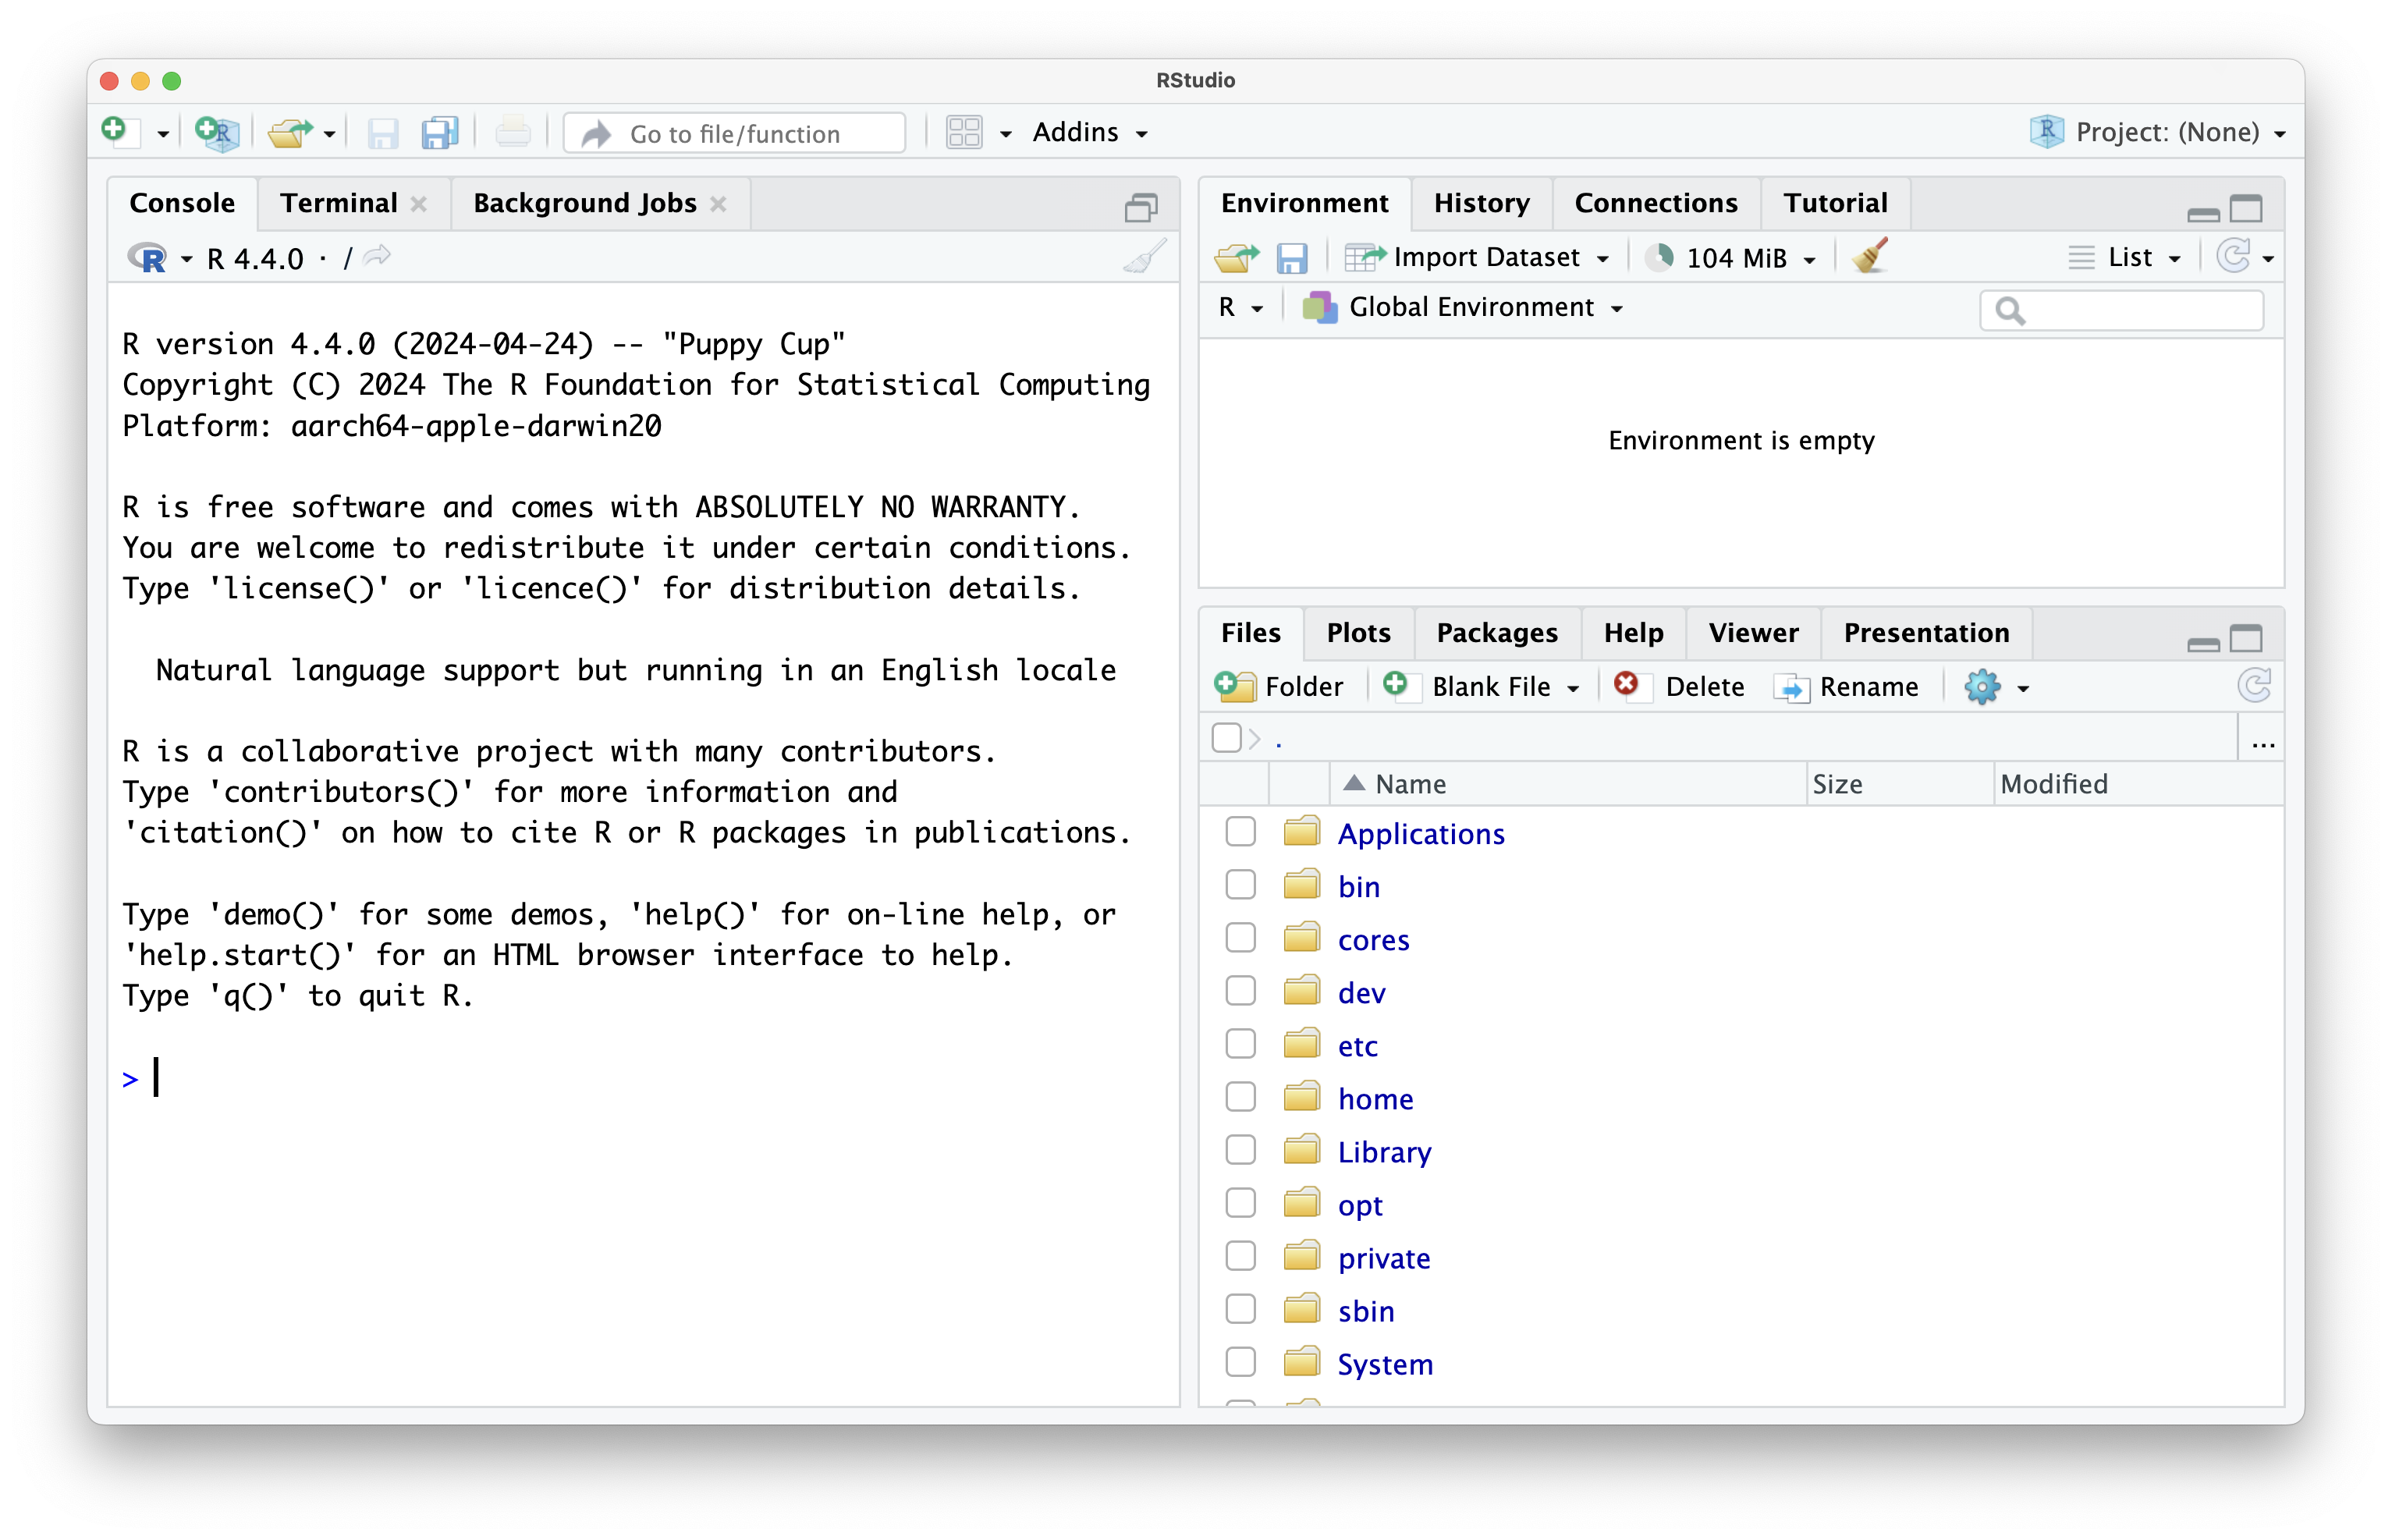
\includegraphics[width=10.22in,height=\textheight]{figures/rstudio_initial.png}

If you go ahead and select \emph{File \textgreater{} New File
\textgreater{} Quarto Document}, type ``My first R'' in the ``Title''
bar and your name in the ``Author'' bar, then your RStudio should look
something like this:

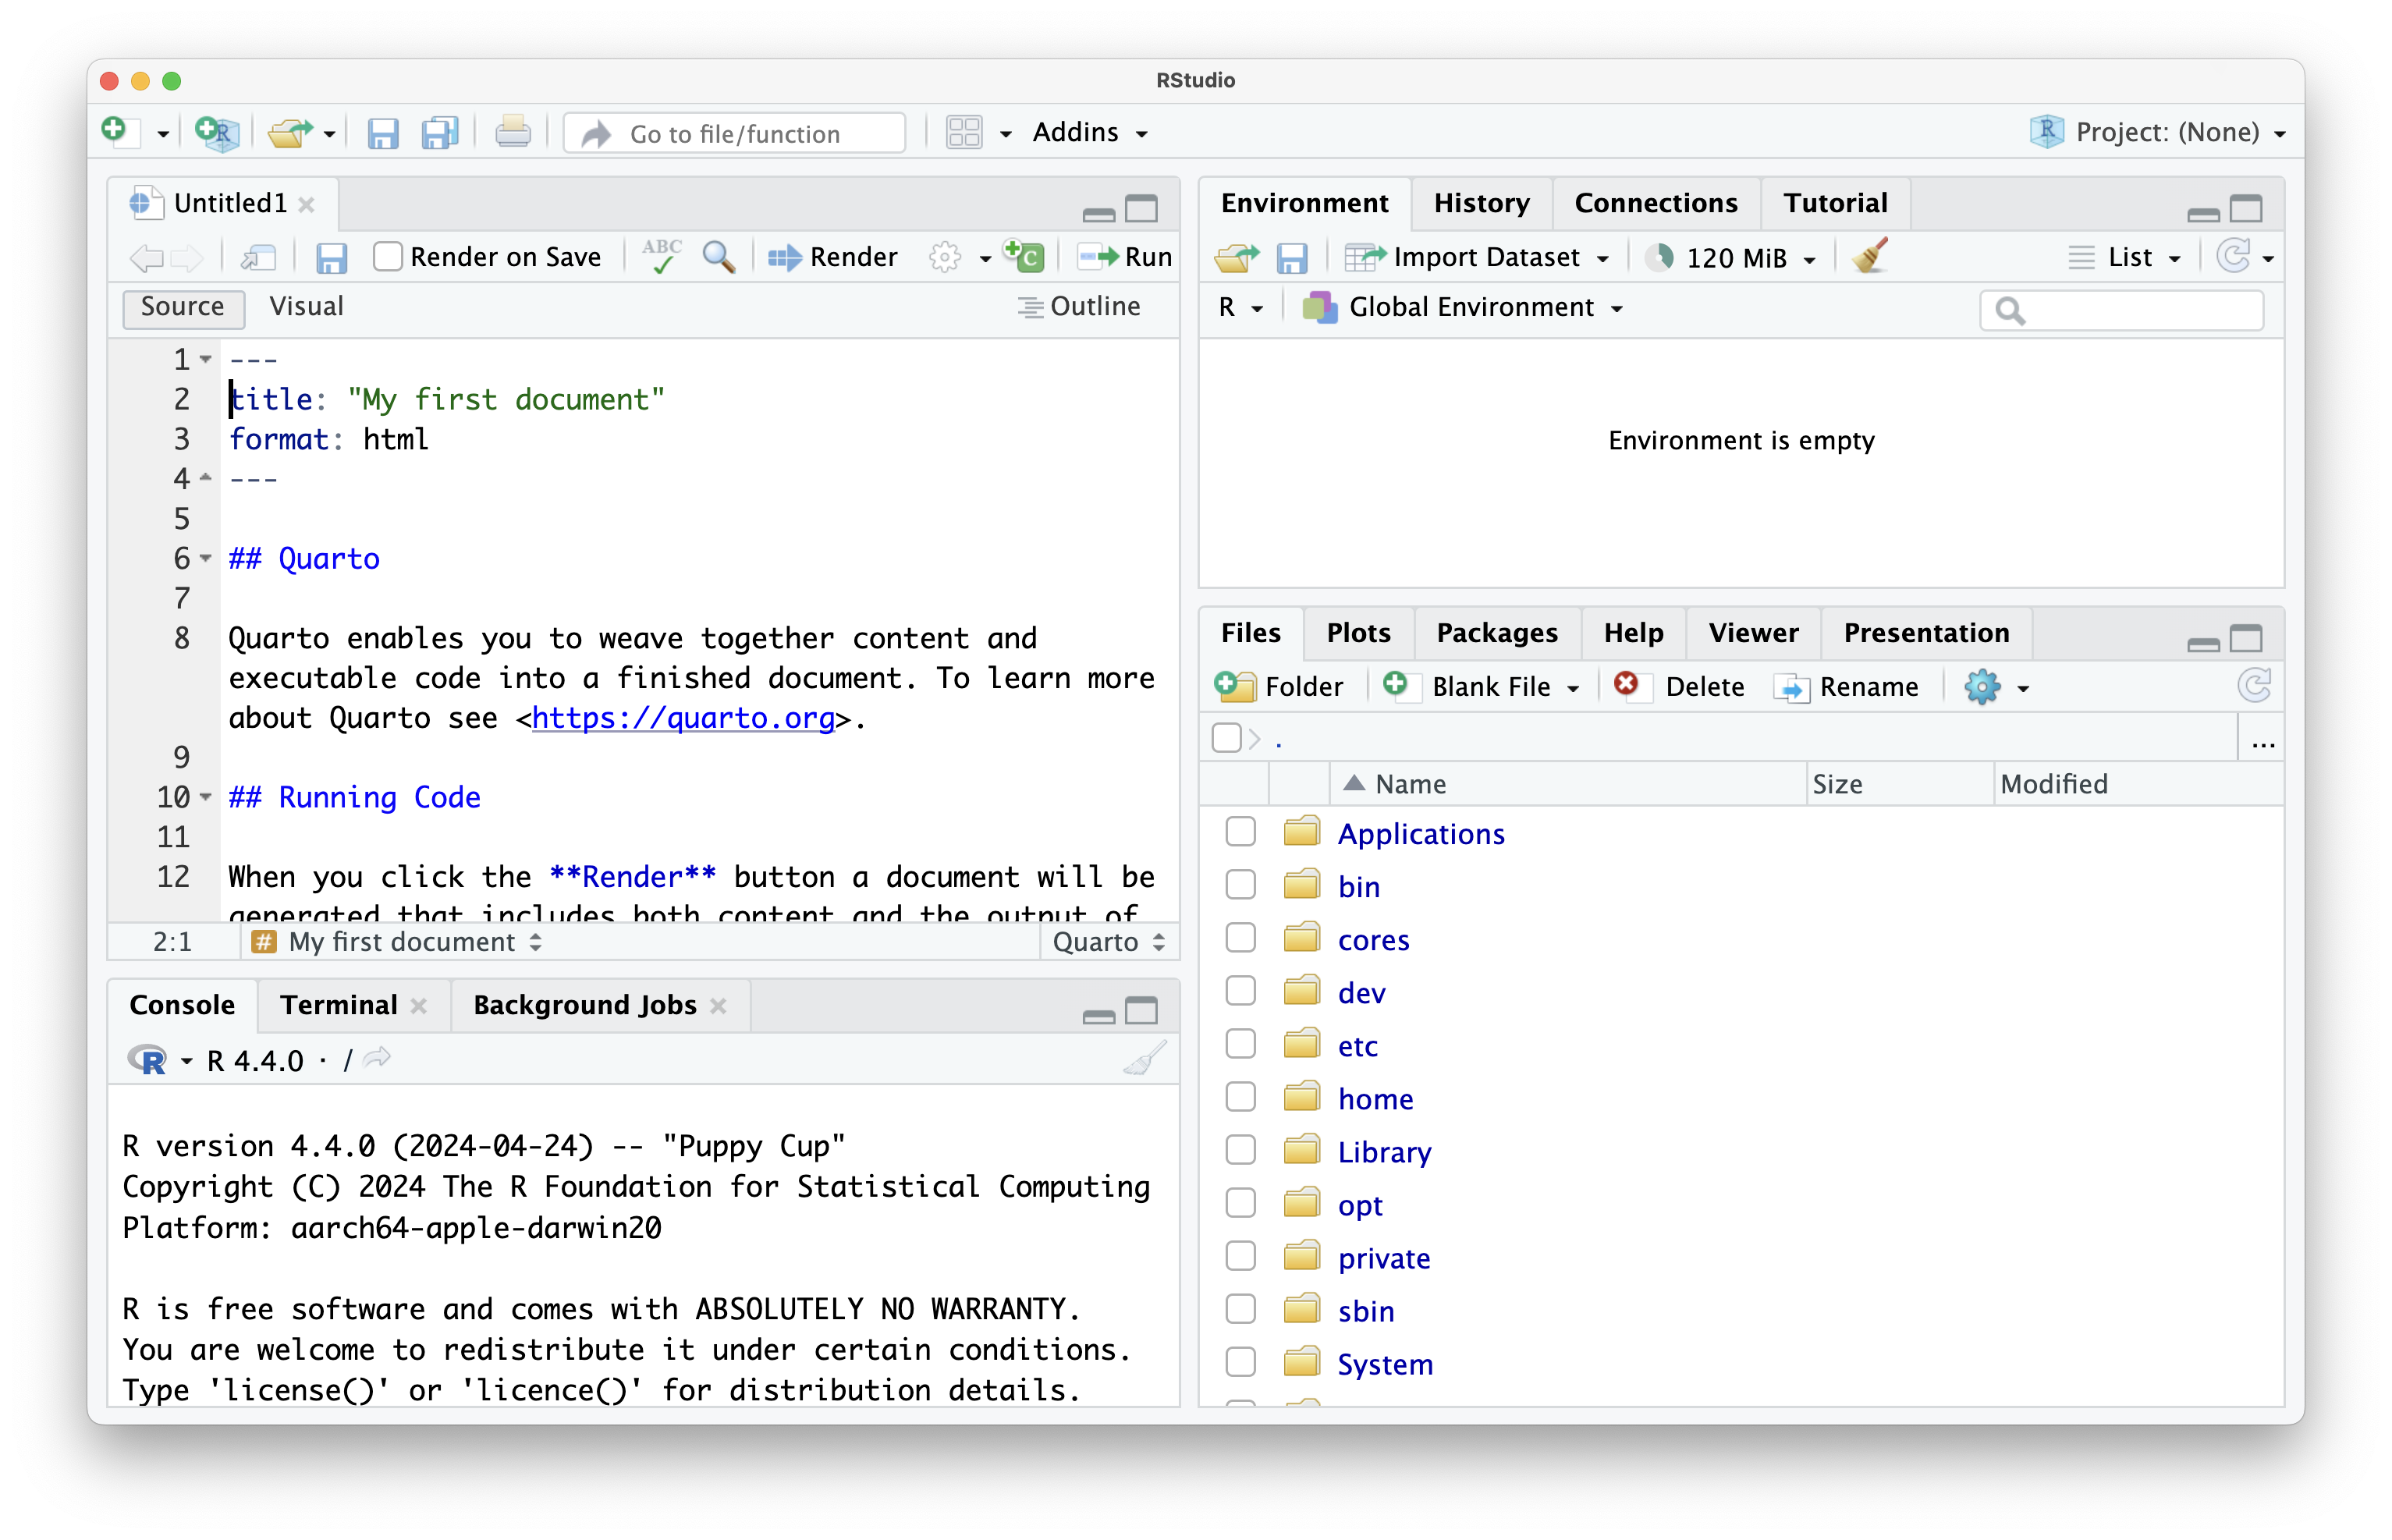
\includegraphics[width=10.22in,height=\textheight]{figures/rstudio_first_doc.png}

Congratulations, you've just created your first R document! Technically,
this is called a \emph{quarto} document, but you can think of it like a
Word document in which you are going to write both regular text and R
code text to tell a data-driven story! We will talk about the contents
of this document in a moment.

If you've used RStudio before, you might have re-arranged the four
panels that you see in the image above, but your version should have the
same general features as in the image above:

\begin{itemize}
\item
  A \textbf{document panel} (the top-left panel in the image), which is
  where the document that you're currently \emph{writing} in lives.
\item
  A \textbf{console panel} (The bottom-left panel in the image), which
  is where we can \emph{run} the code that we write.
\item
  An \textbf{environment panel} (the top-right panel in the image),
  which will show the ``objects'' that exist in your R environment. We
  haven't run any code yet, so this is empty.
\item
  The \textbf{files panel} (which is also the \textbf{plot panel} and
  \textbf{viewer panel}), which shows the files in the current local
  ``directory'' (the folder on your computer). When you first open
  RStudio, this is typically your computer's home page.
\end{itemize}

Note that the size of each panel can be changed by dragging the border
between two adjacent panels.

The most important panels at the moment are the \emph{documents} and
\emph{console} panels on the left, so let's take a closer look at these.

\section{Quarto documents}\label{quarto-documents}

The top-left documents panel contains the document that you're currently
working in. There are several types of documents that you could create
in which you could write your R code, but I recommend using \emph{quarto
documents}.

\begin{tcolorbox}[enhanced jigsaw, rightrule=.15mm, toptitle=1mm, title=\textcolor{quarto-callout-note-color}{\faInfo}\hspace{0.5em}{Quarto versus R Markdown}, leftrule=.75mm, bottomtitle=1mm, colbacktitle=quarto-callout-note-color!10!white, coltitle=black, titlerule=0mm, opacityback=0, colframe=quarto-callout-note-color-frame, arc=.35mm, opacitybacktitle=0.6, bottomrule=.15mm, left=2mm, breakable, toprule=.15mm, colback=white]

If you're already familiar with \emph{R Markdown}, \emph{quarto} is just
its modern successor and at first glance, quarto is pretty much the same
as R Markdown, with minor syntactic differences. Don't worry, if you
already have a bunch of old R Markdown documents, there isn't much to be
gained by converting them to quarto files, but I'd recommend that any
\emph{new} files you create be quarto files rather than R Markdown. If
you've never heard of R Markdown, feel free to forget I even mentioned
it.

\end{tcolorbox}

Quarto documents allow you to combine text and code, so that rather than
having your R code be lonely on its own, your code (and its output) can
instead live nestled in between narrative text that describes the
analysis that you're conducting and summarizes the results you obtain.

Quarto documents are mind-blowingly versatile, and while they are mostly
used to create simple html or pdf documents, they can also be used to
make websites (like \href{www.rebeccabarter.com}{mine}) and books (like
this one!)

Whenever I am conducting an analysis using R, I conduct my analysis in a
quarto document. In fact, every chapter in this book is just a quarto
document!

Since we want to practice \emph{reproducible} data science, it is
important that we keep detailed records of the code we wrote that led us
to our data-driven answers. Quarto provides us with an easy way of doing
that. Moreover, because you can surround your code with text narrative,
it can be used to communicate your analysis and results to other people:
quarto lets us feed two birds with one seed!

To start a new quarto document inside RStudio:

\begin{itemize}
\tightlist
\item
  Hit the ``New file'' icon, , in the top-left-hand corner of RStudio
  (or \emph{File \textgreater{} New File \textgreater{} Quarto
  Document}) and select ``Quarto document''. The following window should
  pop up:
\end{itemize}

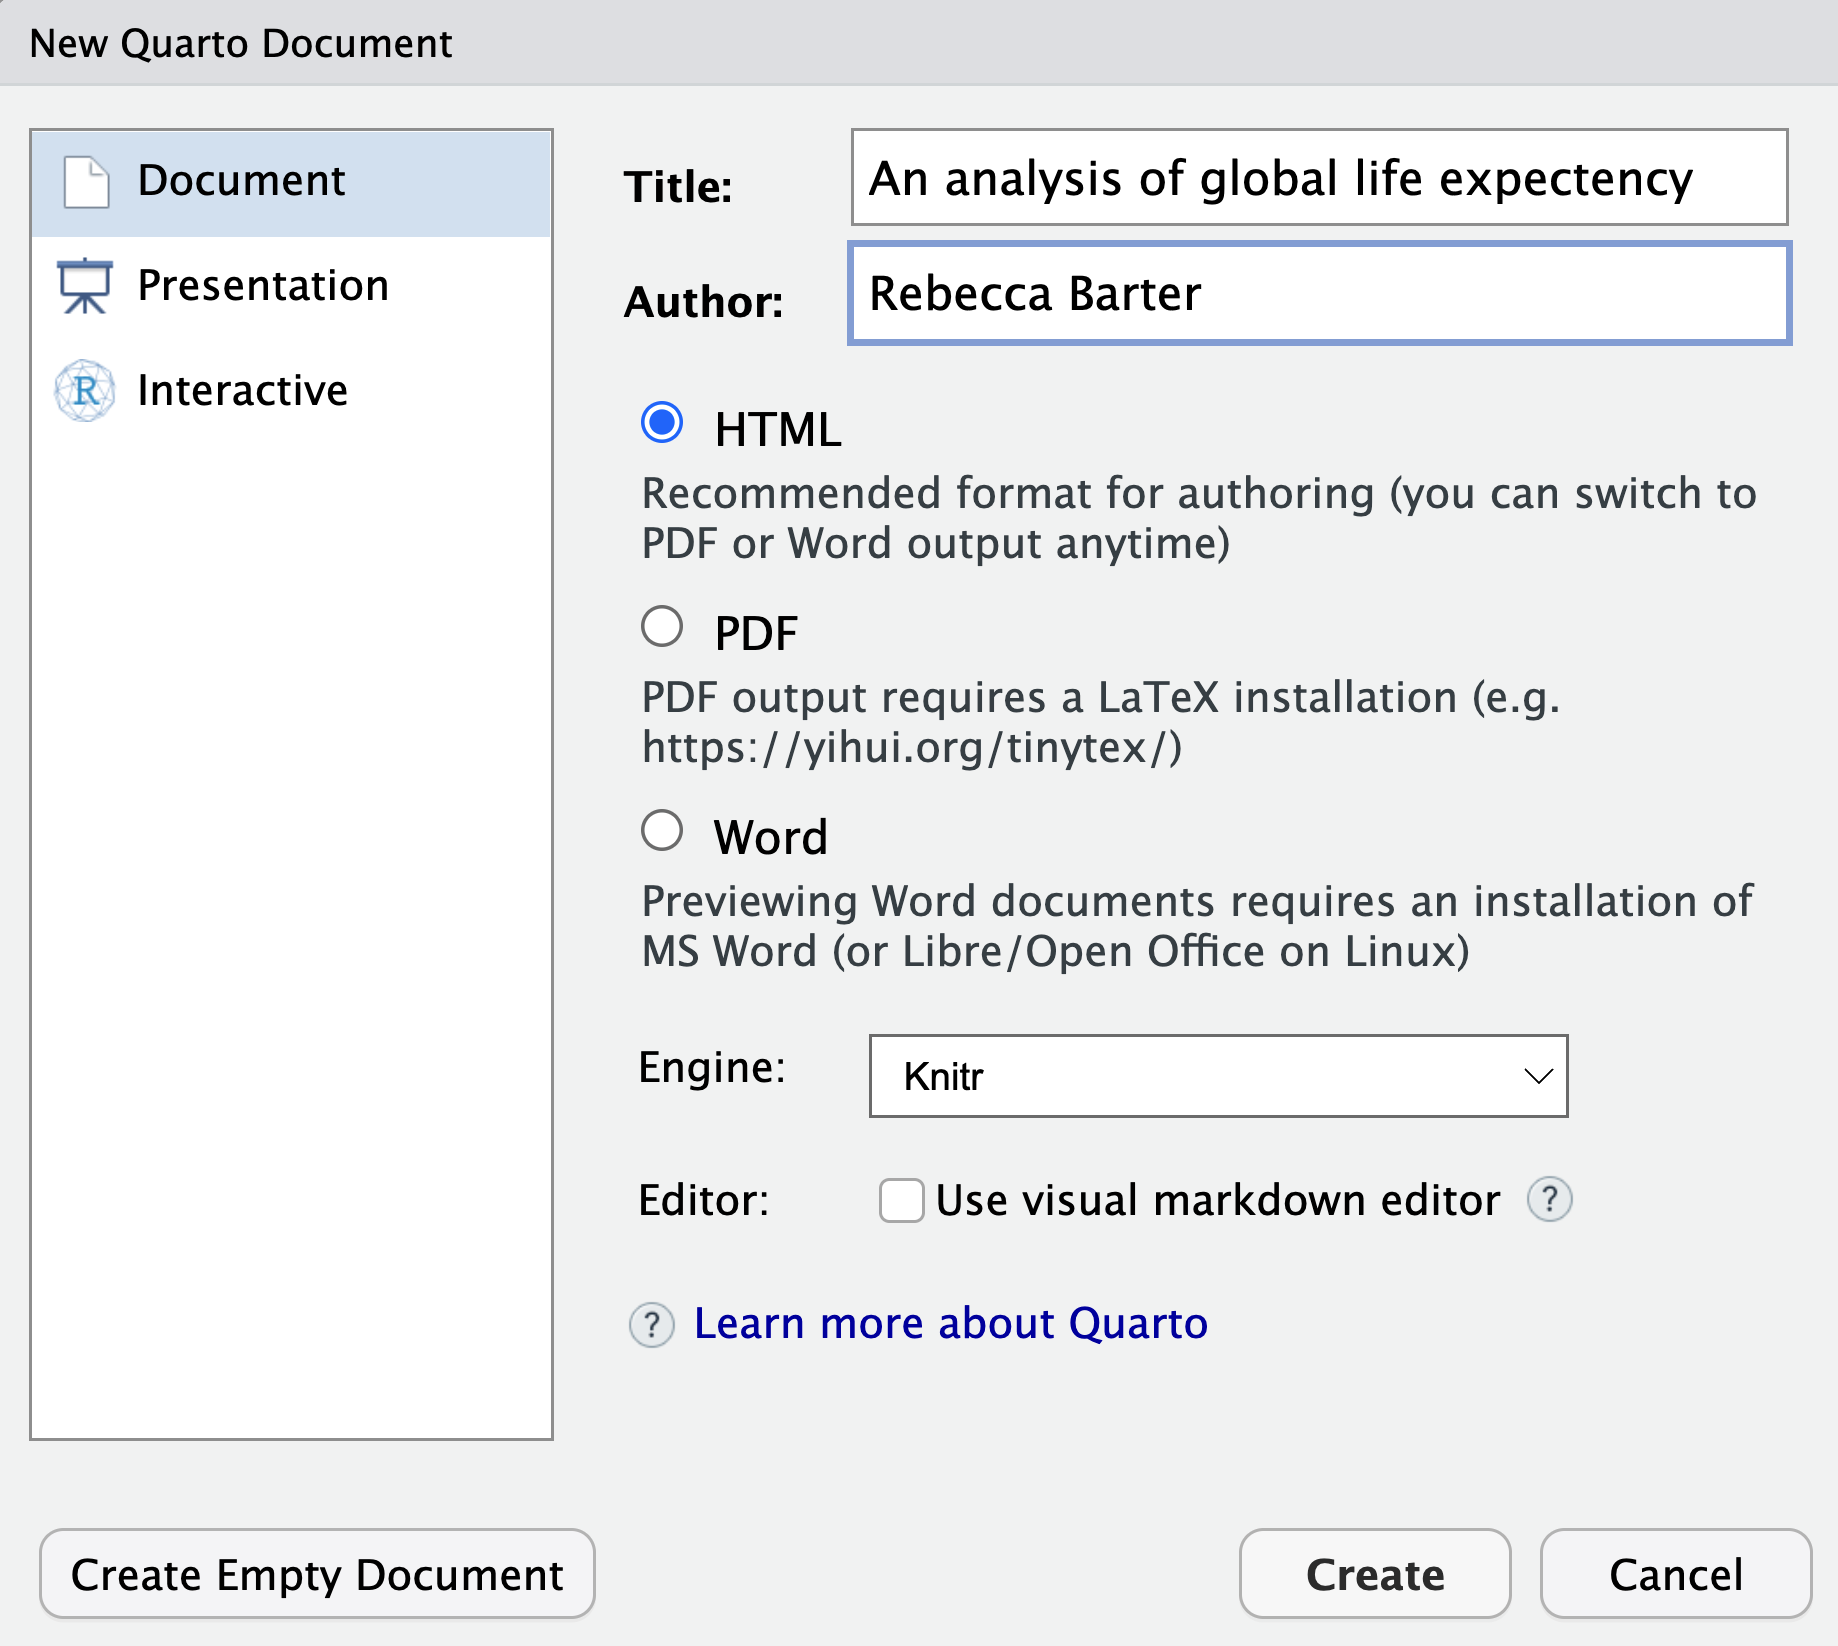
\includegraphics[width=6.13in,height=\textheight]{figures/new_quarto.png}

Then

\begin{itemize}
\item
  Choose a title (e.g., ``An analysis of global life expectancy''), and
  make yourself the author.
\item
  Hit the ``\emph{Create}'' button to create your file.
\end{itemize}

This will open up a new quarto template document in the documents panel.

The template text in your new quarto document contains a very summary of
how quarto documents work. Take a moment to read it.

The regular white-background text is just text like in a Word Document.
The text at the top of the quarto document surrounded by dashes
\texttt{-\/-\/-} is called the \textbf{YAML header}, provides several
parameters and options for your quarto document, such as the title, the
author, and the rendered output format (more on this in a moment).

The grey boxes with \texttt{\{r\}} are called ``code chunks'' and these
are where we will write your R code.

\subsection{Rendering quarto
documents}\label{rendering-quarto-documents}

Note the instructions in the template quarto document ``\emph{When you
click the \textbf{Render} button a document will be generated that
includes both content and the output of embedded code}.'' Take the
document's advice: click the ``Render'' button with a blue arrow, which
is circled in orange below and save your document when prompted as
``analysis.qmd'' or something like that:

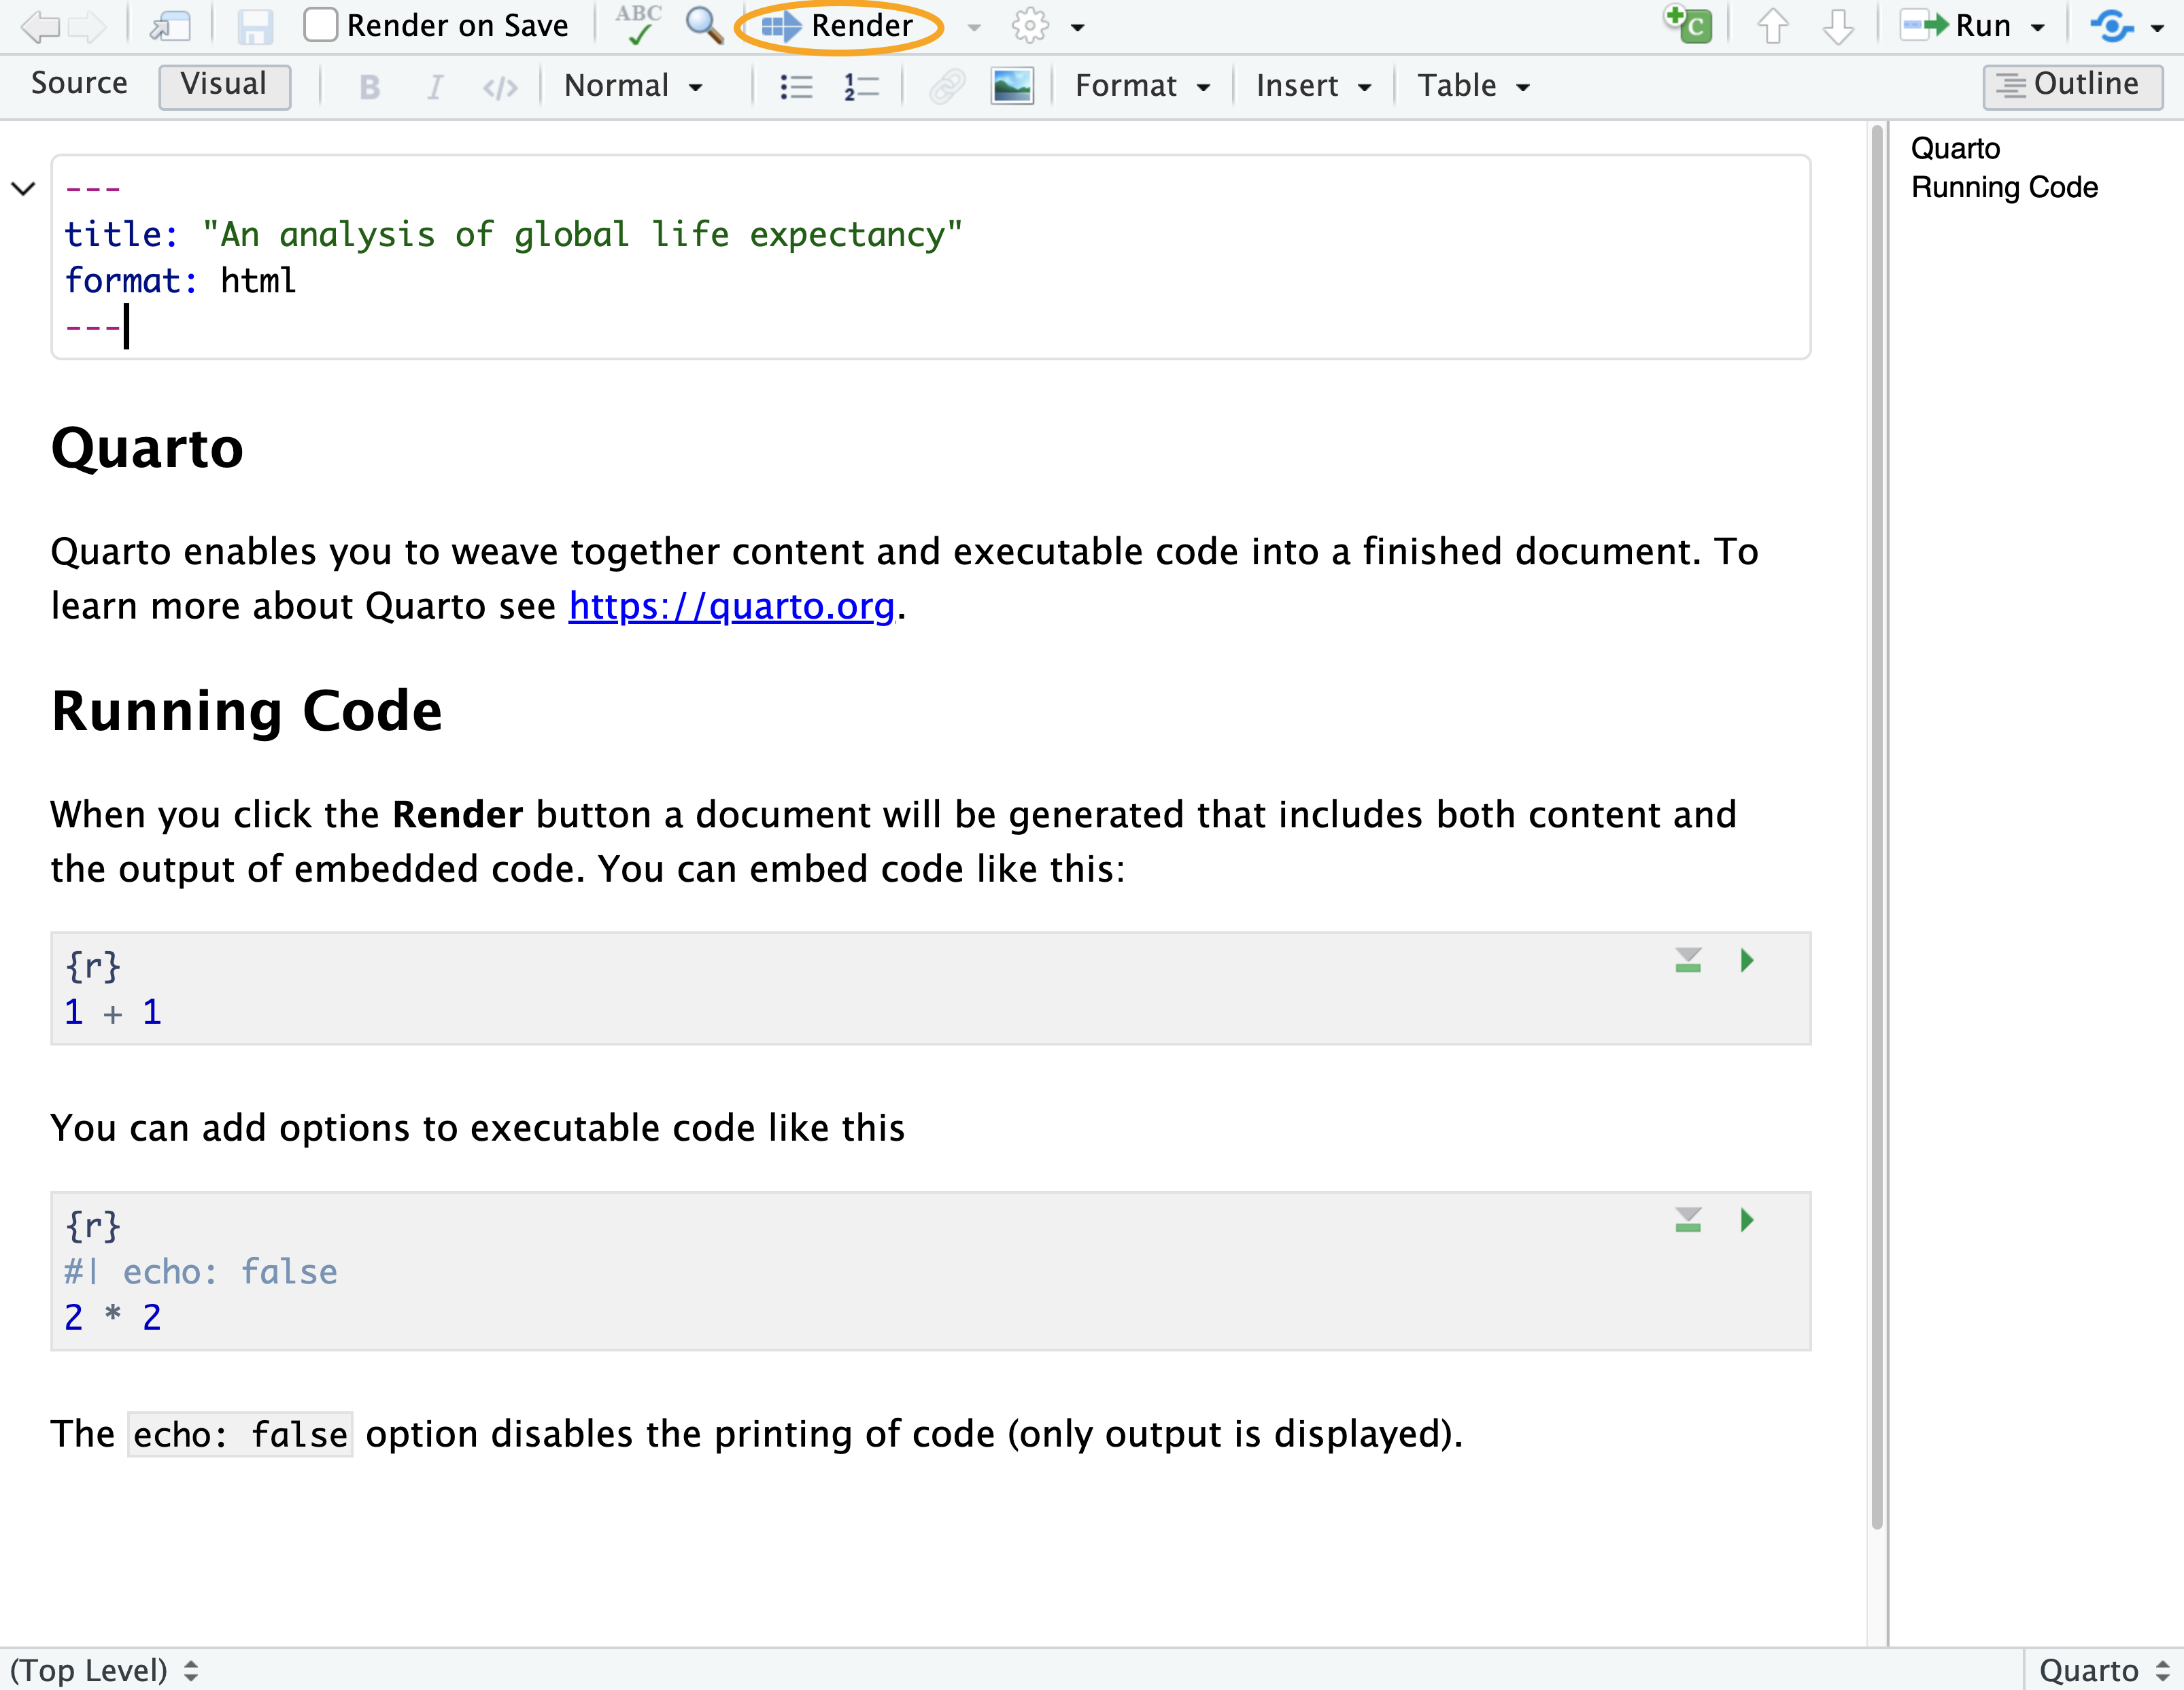
\includegraphics[width=10.71in,height=\textheight]{figures/render.png}

Hopefully, what happened when you hit ``Render'' is that some text
appeared very quickly in your bottom-left ``console'' panel and your web
browser opened up with a new (html) webpage with whatever title you
provided that looks something like this:

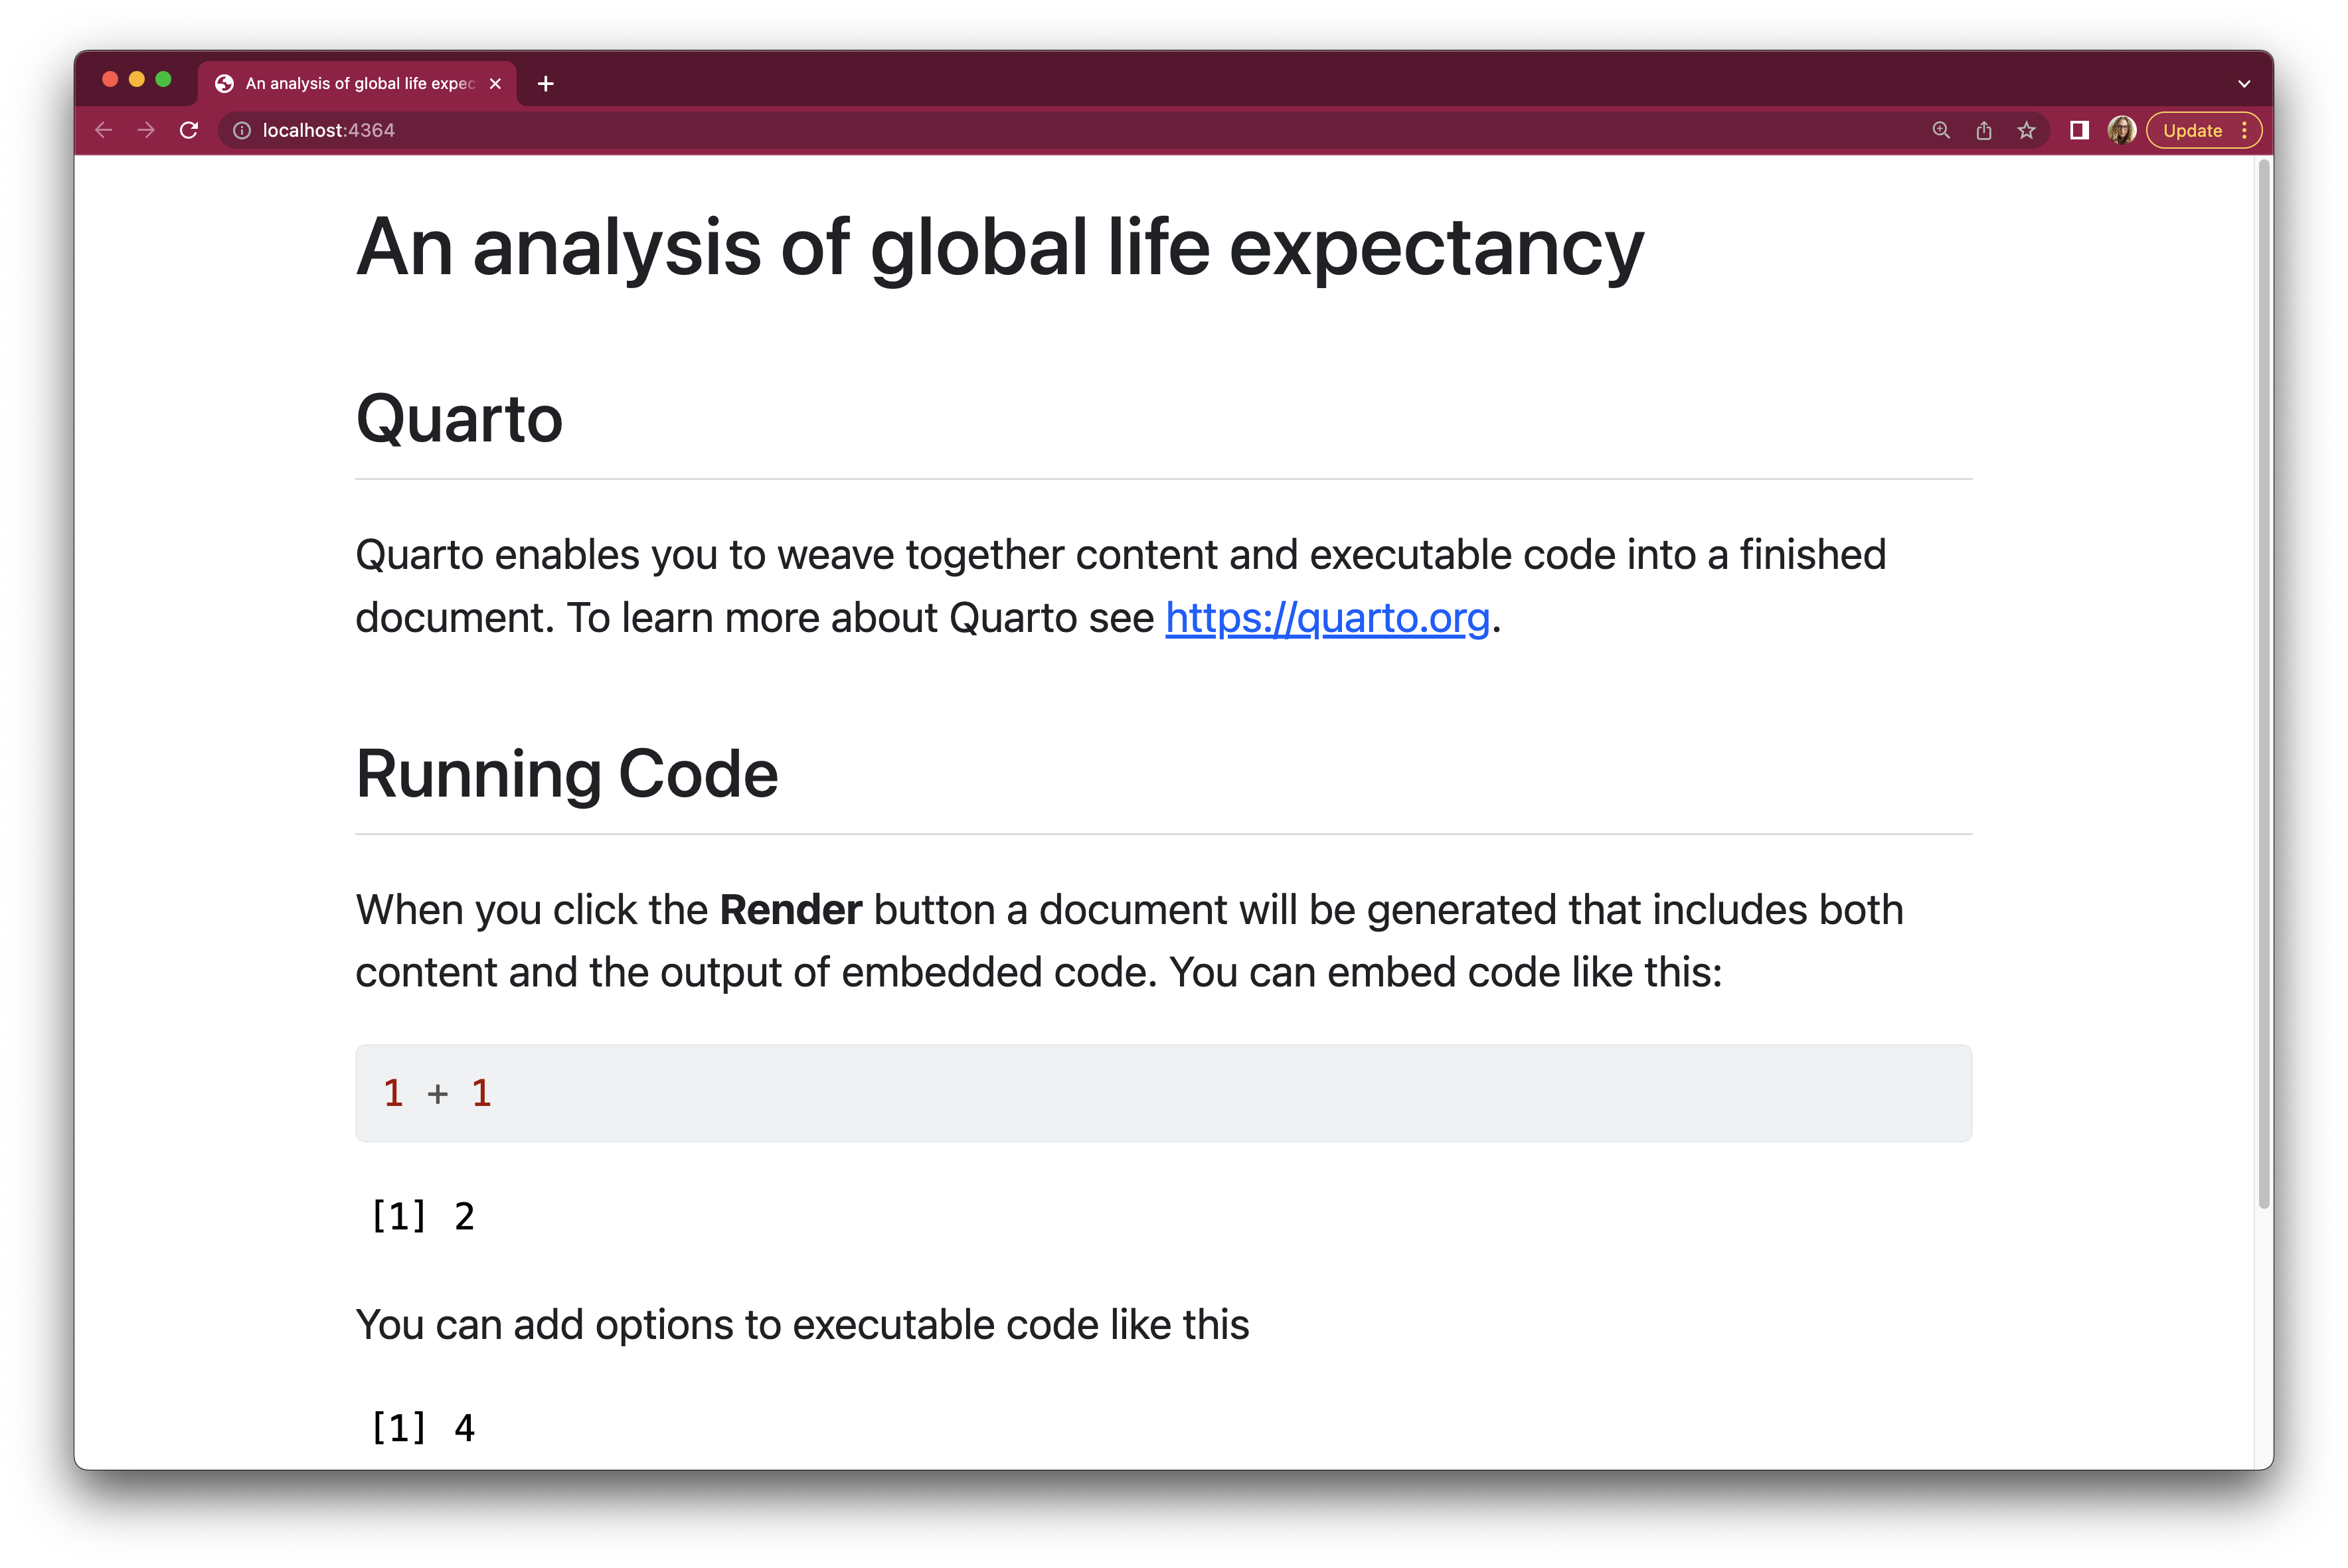
\includegraphics[width=11.79in,height=\textheight]{figures/render_doc.png}

If you're using RStudio in the cloud (or you have different settings to
me), you may have instead found that the window opened in the ``Viewer''
panel of your RStudio application. If no window opened anywhere,
navigate to the location on your computer where you saved your quarto
document (``analysis.qmd'') and see if a new file ``analysis.html'' has
appeared. If it has, open it in your web browser.

What happened when we hit the ``Render'' button? Hitting ``Render''
renders your \emph{interactive} quarto (analysis.qmd) document as a
\emph{static} HTML (analysis.html) file. This is like saving your
interactive word document file that you can edit as a static pdf file
that you cannot edit.

Compare the original quarto (analysis.qmd) document in RStudio with the
rendered page (analysis.html) in your web browser. What differences do
you notice? Which one can you modify?

\begin{tcolorbox}[enhanced jigsaw, rightrule=.15mm, toptitle=1mm, title=\textcolor{quarto-callout-tip-color}{\faLightbulb}\hspace{0.5em}{Rendering quarto as PDF and Microsoft Word documents}, leftrule=.75mm, bottomtitle=1mm, colbacktitle=quarto-callout-tip-color!10!white, coltitle=black, titlerule=0mm, opacityback=0, colframe=quarto-callout-tip-color-frame, arc=.35mm, opacitybacktitle=0.6, bottomrule=.15mm, left=2mm, breakable, toprule=.15mm, colback=white]

By default, quarto documents will be rendered as HTML files, but they
can also be rendered to PDF and Microsoft Word files! You can do this by
changing the \texttt{format:\ html} in the ``\emph{yaml}'' text at the
top of your quarto document (right underneath the ``title'' and
``author'' definitions) to \texttt{format:\ pdf} or
\texttt{format:\ docx}, respectively.

However, note that to render a quarto document to a PDF file, you will
need to have an application called LaTeX installed on your computer (see
the exercise below).

If you switched to \texttt{format:\ pdf}, we recommend switching back to
\texttt{format:\ html} for the rest of this lesson.

\end{tcolorbox}

\subsection{``Visual'' mode versus ``Source''
mode}\label{visual-mode-versus-source-mode}

There are currently two modes that your \emph{interactive} quarto
document (i.e., the version in RStudio, not the rendered HTML document)
can be in.

The ``analysis.qmd'' file in ``visual mode'' looks like this:

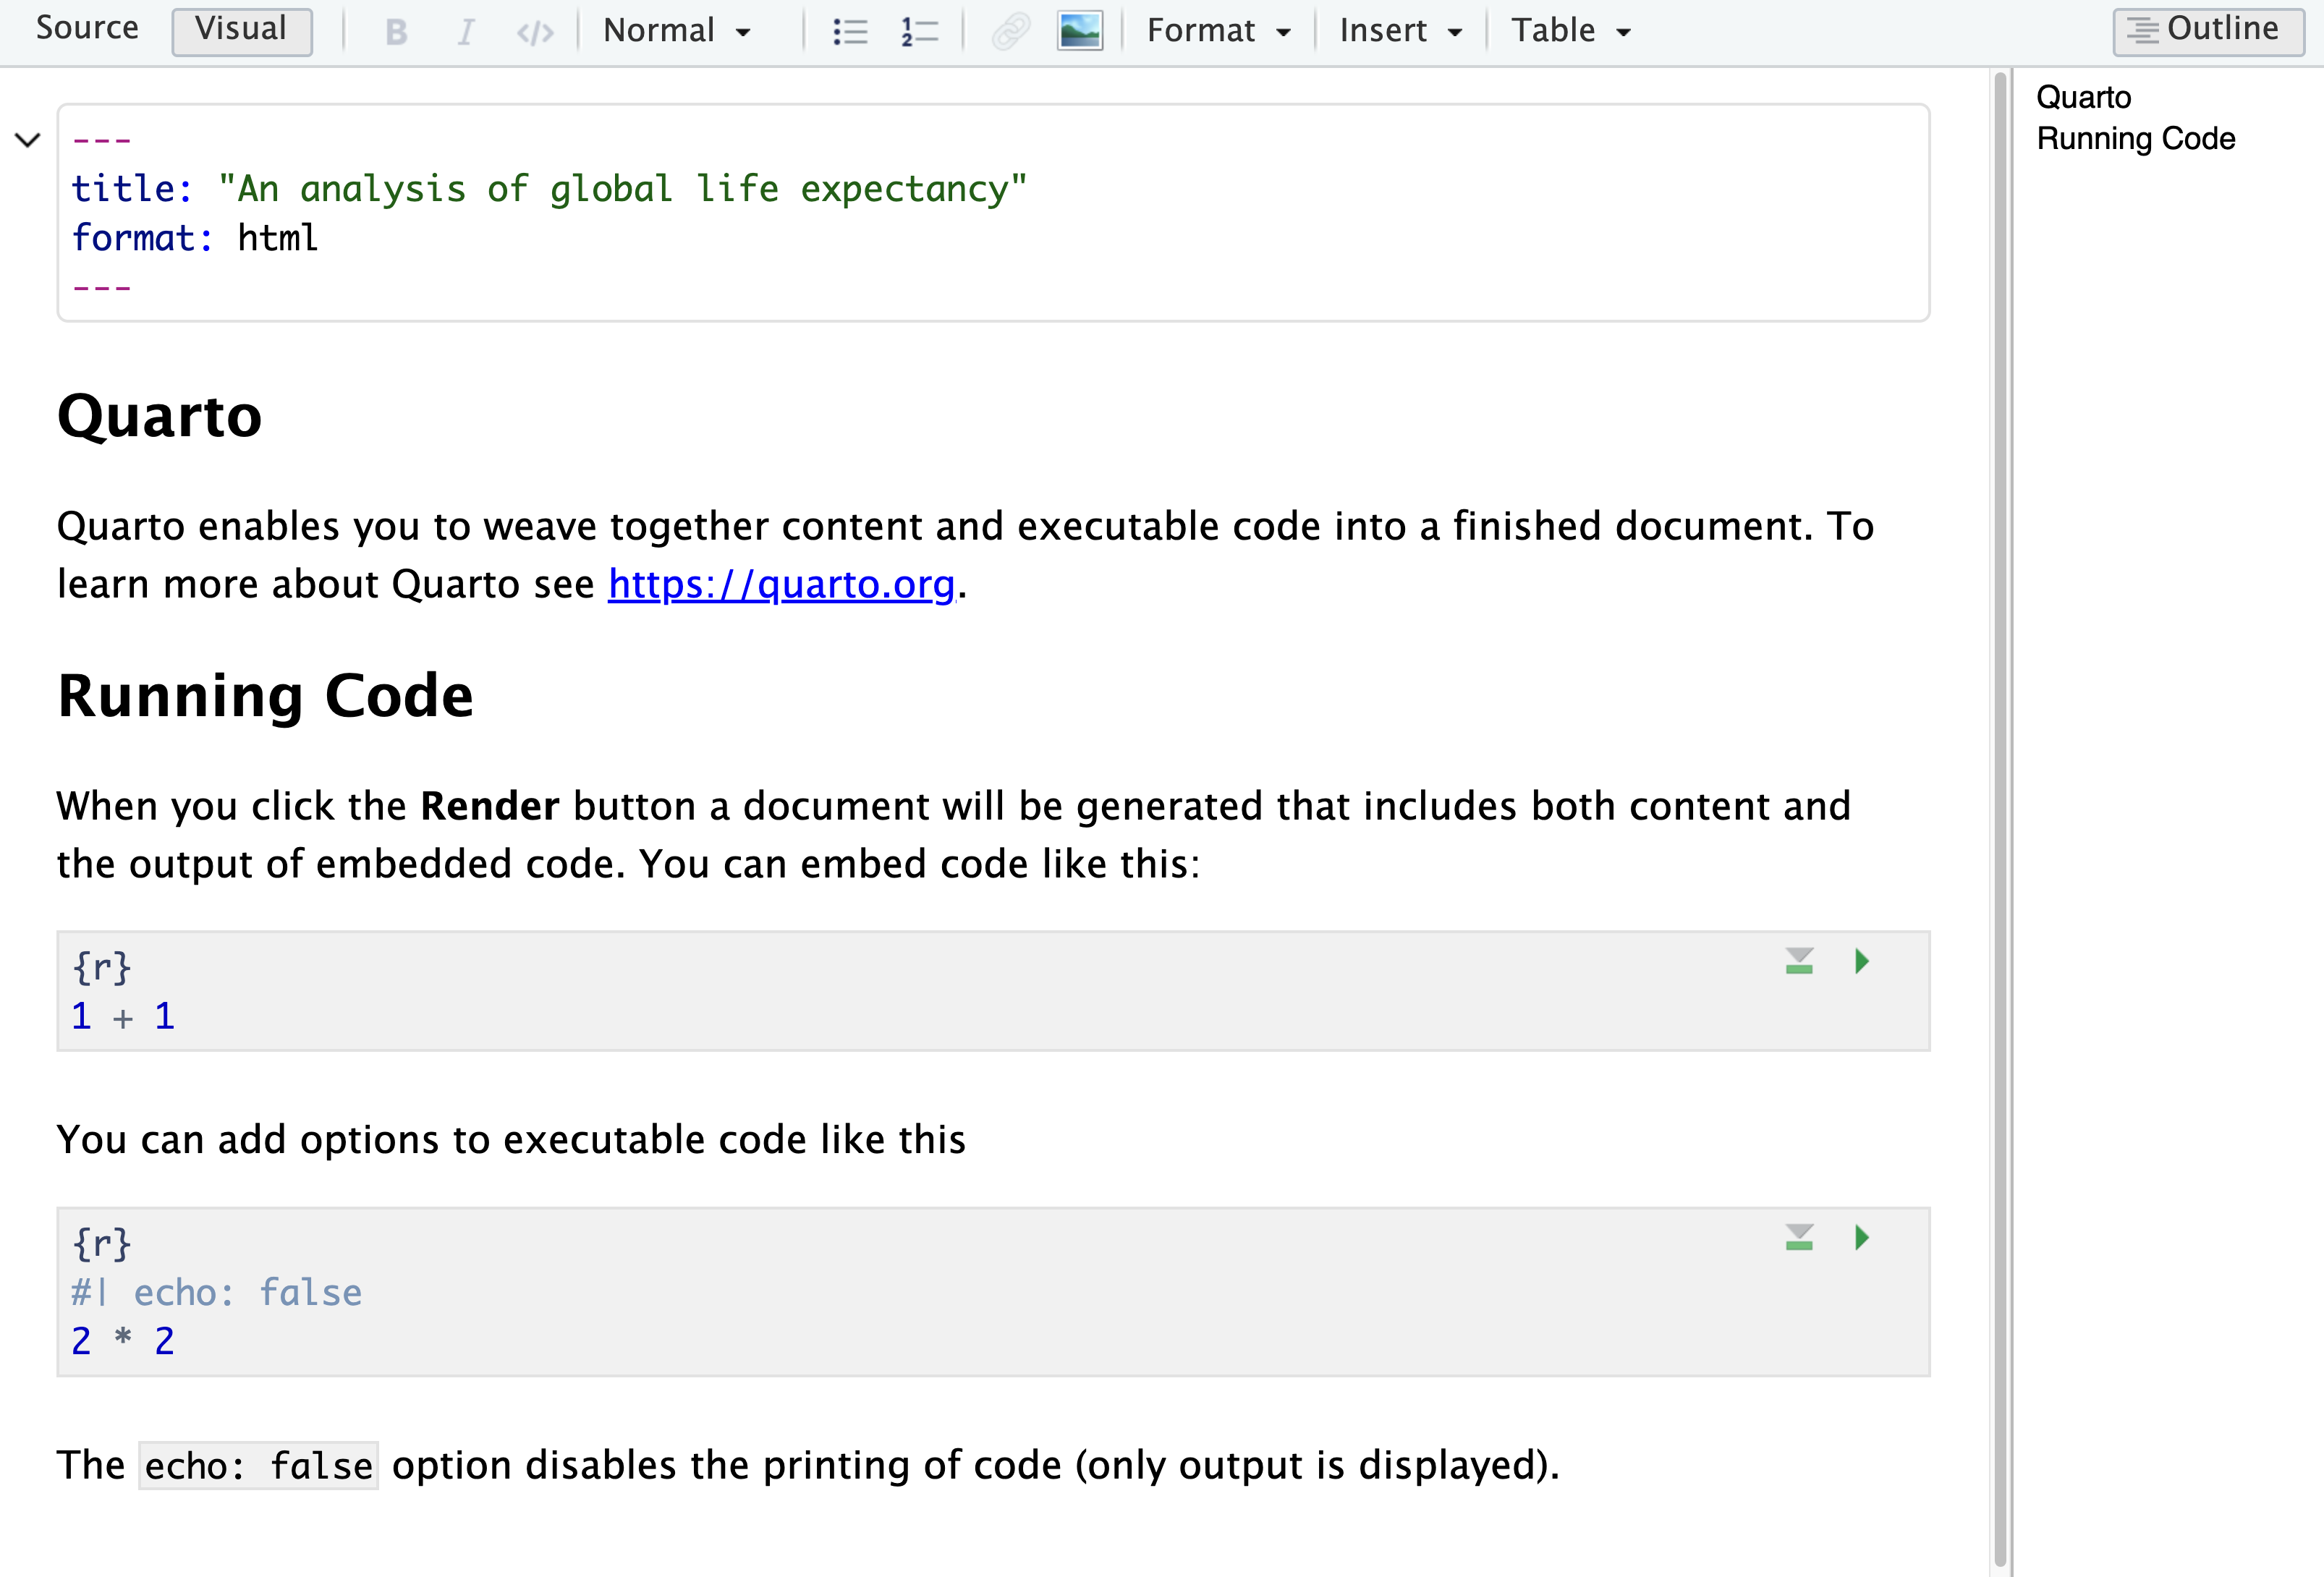
\includegraphics[width=10.71in,height=\textheight]{figures/visual.png}

If your quarto document is in visual mode, it will be a lot more like a
Word Document, where you will see boldface text, headings, italics,
links, etc.

In this visual mode format, much of the underlying quarto syntax is
hidden from you.

Alternatively, if you view this same ``analysis.qmd'' quarto document in
``Source'' mode, you will be looking at the underlying quarto (markdown)
syntax. The ``analysis.qmd'' file in source mode looks like this:

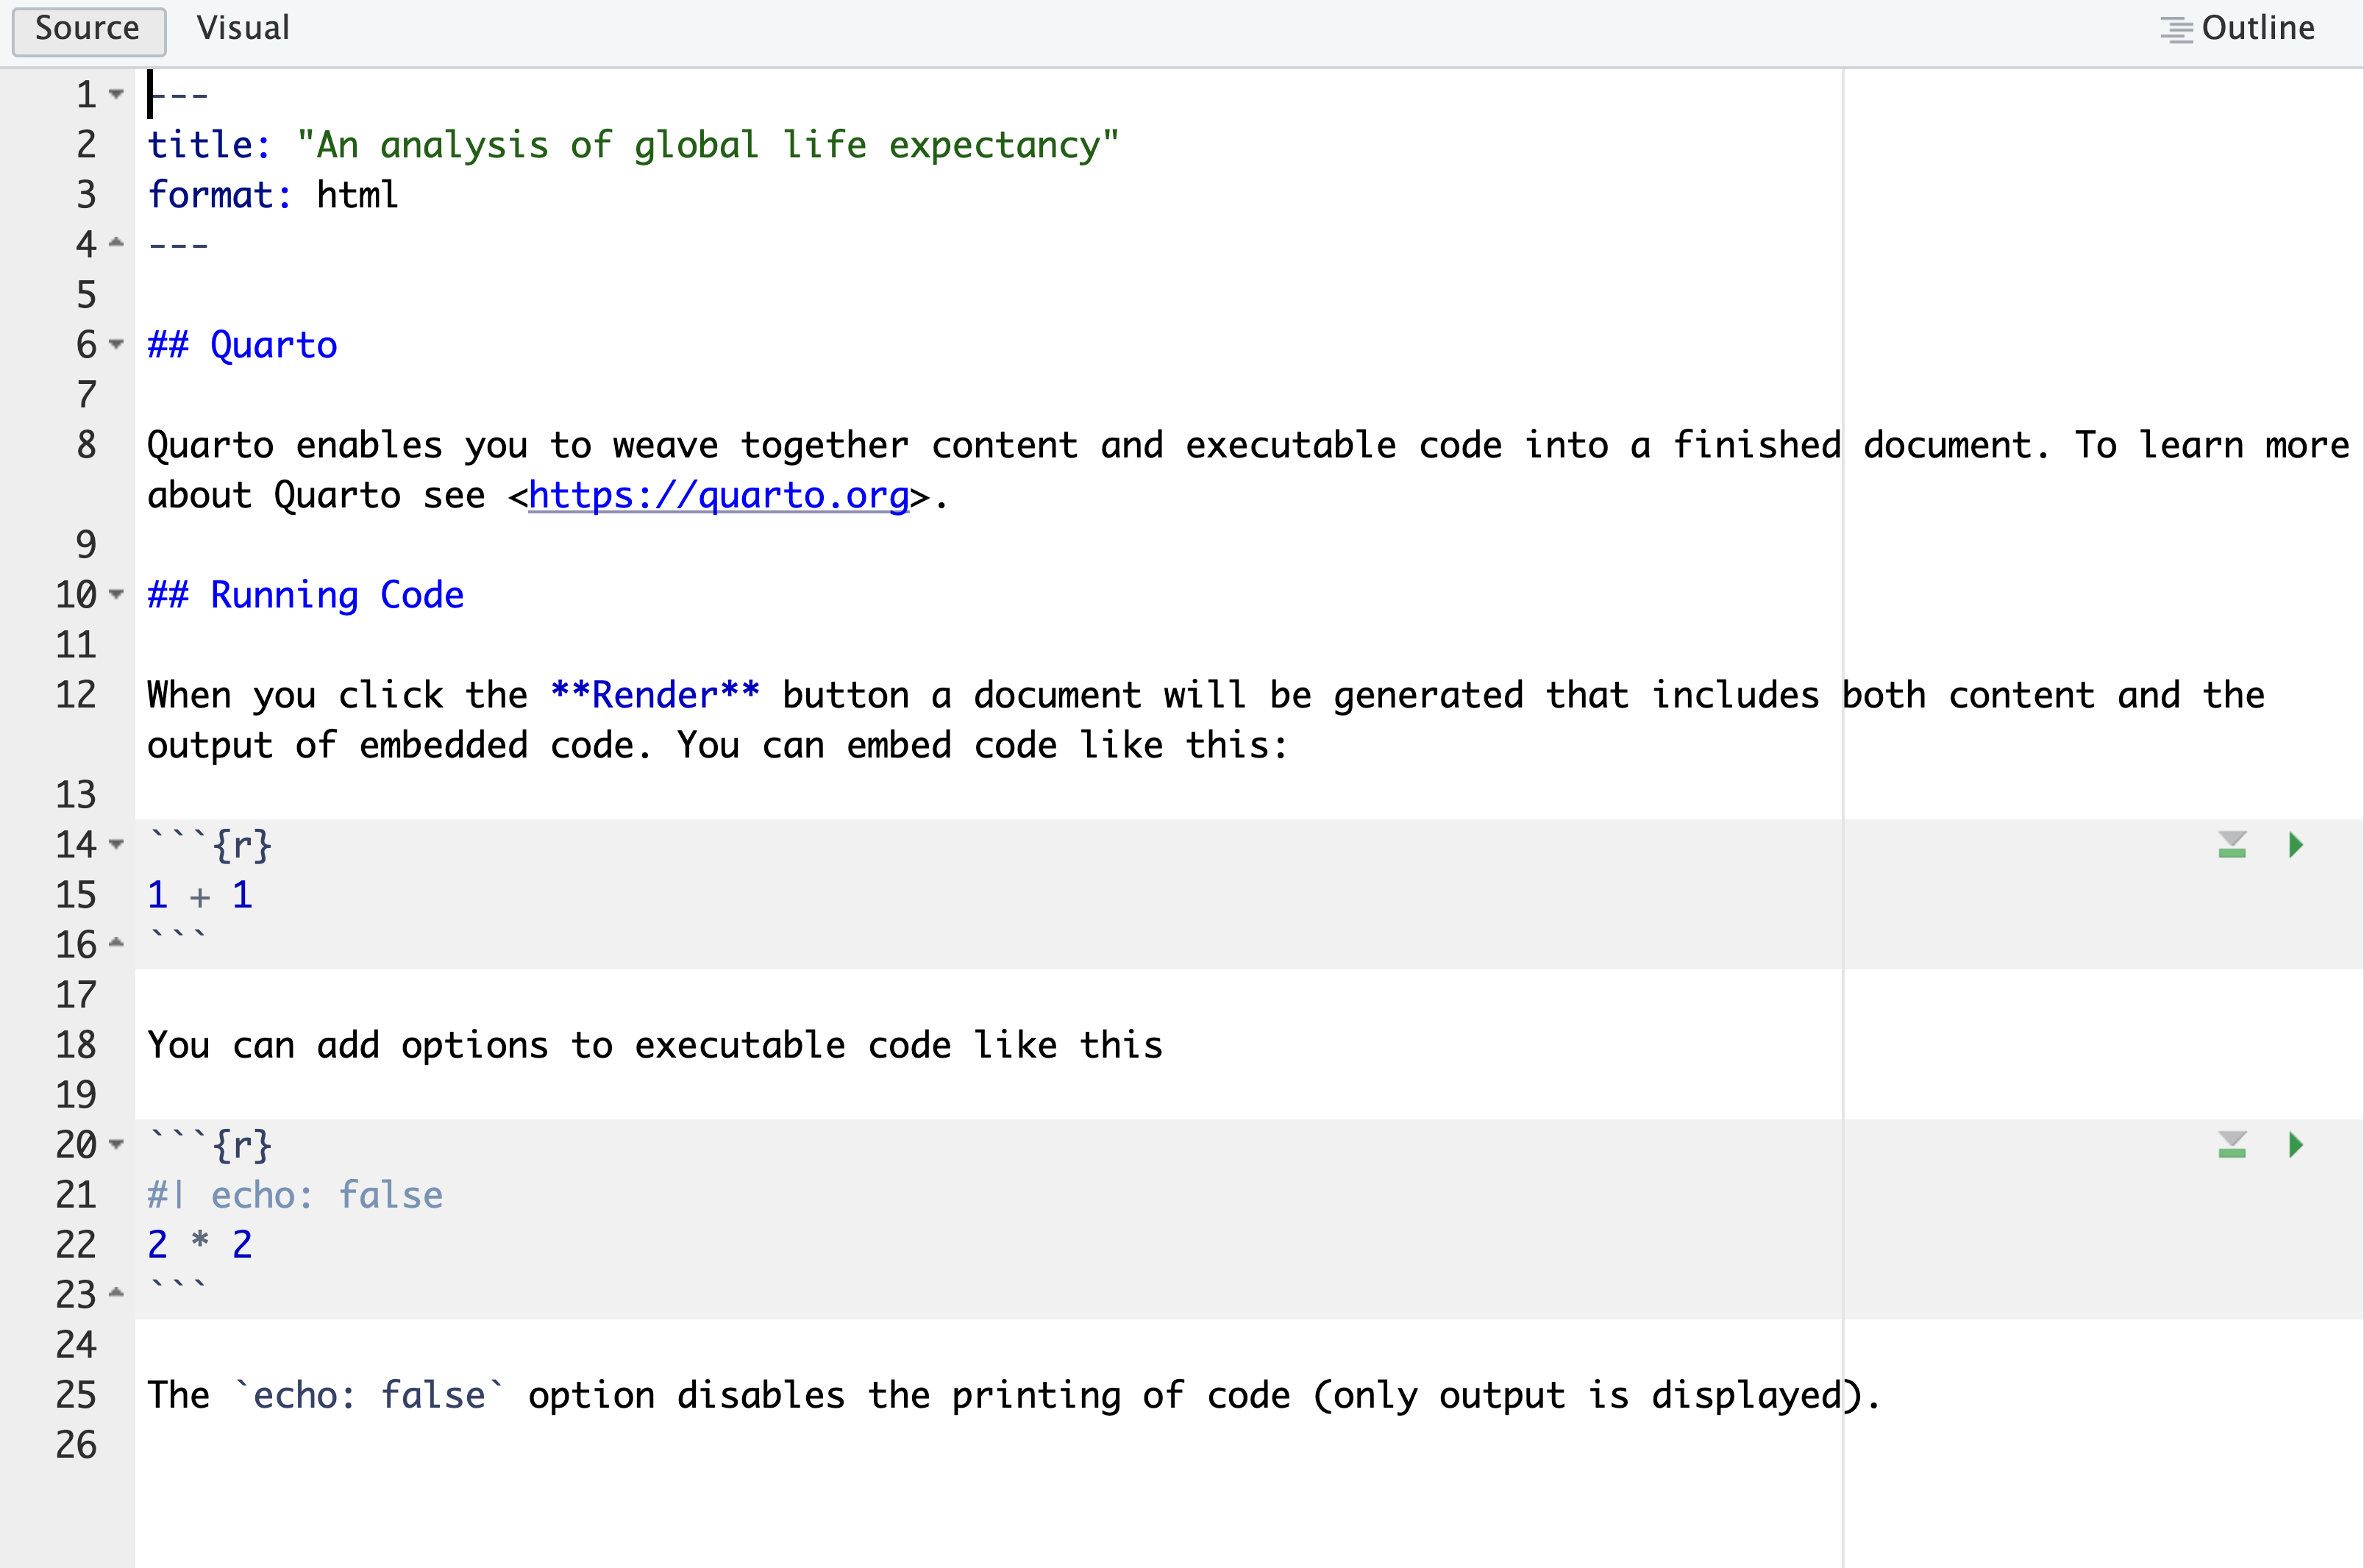
\includegraphics[width=10.71in,height=\textheight]{figures/source.png}

Notice that there is no boldface text, or headings, etc. Instead there
are raw text symbols to represent these things. For instance,
surrounding text by two asterisks (**) creates boldface text and
preceding some text with pound symbols (\#\#) creates headings (the more
pound symbols used, the more lower-level the heading). This text syntax
is called ``Markdown'' syntax.

Can you identify whether your quarto document is currently in source or
visual mode?

You can toggle your quarto document between source and visual mode using
the ``Source'' and ``Visual'' buttons in the top-left corner of your
quarto document in RStudio.

Whether you prefer source or visual mode will come down to a personal
preference. I personally prefer working with the source mode where I can
see the underlying Markdown syntax that defines the text formatting and
R code chunks, but I know many people who prefer the visual mode.

\subsubsection{Markdown syntax}\label{markdown-syntax}

In case you're interested in learning a little bit more about Markdown
syntax, switch your document over to the ``Source'' mode by hitting
``Source'' in the top left corner of your document.

Re-render your document by hitting the ``Render'' button, and based on
the rendered static html page that will open in your web browser, let's
try to make some sense of the Markdown syntax used in the original
quarto (.qmd) document in RStudio.

Can you see what the \texttt{\#\#} syntax is doing (if you can't see the
\texttt{\#\#} syntax in your quarto document in RStudio, ensure that you
are viewing the quarto document using ``Source'' rather than ``Visual''
in the top-right corner of the document)? The pound symbols are
\textbf{markdown} syntax for creating headers: \texttt{\#} will create a
top-level header (this is the same level as the overall document title),
\texttt{\#\#} will create a level-2 header, \texttt{\#\#\#} will create
a level-3 header, etc.

Notice that the word ``\textbf{Render}'' is shown in bold in the
rendered html file. By looking at the .qmd file, can you figure out what
the markdown syntax is for creating bold-face text?

To learn more about markdown syntax, see
\url{https://www.markdownguide.org/basic-syntax/}.

If you want to play around with the Markdown formatting syntax, add some
additional markdown features to your \texttt{analysis.qmd} file (E.g., a
sub-section heading, some italics, or extra bold text), and re-render
your quarto html output by hitting the ``Render'' button. Take note of
how the changes you made were rendered in the static HTML version of
your document.

\section{Where to write your code}\label{where-to-write-your-code}

\subsection{Writing R code in code chunks in a quarto
document}\label{writing-r-code-in-code-chunks-in-a-quarto-document}

I recommend that you write 99\% of your R code in a quarto document,
specifically, your R code should live in the grey boxes with
\texttt{\{r\}}--these are called ``\textbf{code chunks}''.

Hopefully when you were comparing your interactive quarto document with
the rendered HTML document, one difference that you noticed that the
rendered document also showed the ``output'' of the two R code chunks,
which contained the R code \texttt{1\ +\ 1} and \texttt{2\ +\ 2} (the
\emph{output} of these two code chunks were \texttt{2} and \texttt{4},
respectively.)

The image below shows how this interactive code chunk looks in the
quarto document (in source mode):

\begin{Shaded}
\begin{Highlighting}[]
\InformationTok{\textasciigrave{}\textasciigrave{}\textasciigrave{}\{r\}}
\InformationTok{1 + 1}
\InformationTok{\textasciigrave{}\textasciigrave{}\textasciigrave{}}
\end{Highlighting}
\end{Shaded}

Which you can compare with the following image that shows how the static
code chunk looks in the rendered HTML document:

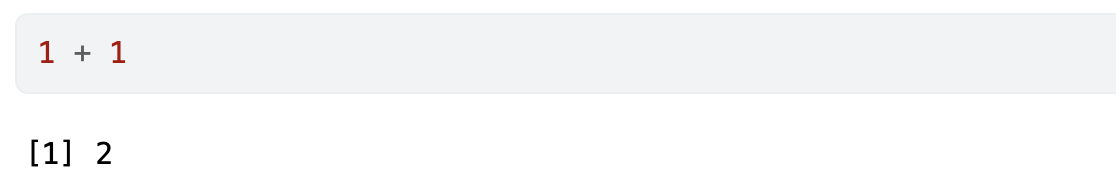
\includegraphics[width=3.72in,height=\textheight]{figures/chunk_html.png}

When a quarto document is rendered into a HTML document, the code in
each of the code chunks is compiled and the result or ``output'' (in
this case the result is \texttt{2}) is printed underneath the chunk.

You can provide ``options'' to code chunks, which are specified with a
point symbol followed by a vertical bar on the first line(s) of the
quarto chunk \texttt{\#\textbar{}}, such as
\texttt{\#\textbar{}\ echo:\ false}, which will tell quarto that it
should hide the R code, but still show the output. So if I have this in
my interactive quarto document in RStudio:

\begin{Shaded}
\begin{Highlighting}[]
\InformationTok{\textasciigrave{}\textasciigrave{}\textasciigrave{}\{r\}}
\InformationTok{\#| echo: false}
\InformationTok{1 + 1}
\InformationTok{\textasciigrave{}\textasciigrave{}\textasciigrave{}}
\end{Highlighting}
\end{Shaded}

I will only see this in the rendered HTML document (i.e., the
\texttt{1\ +\ 1} code is hidden):

\begin{verbatim}
[1] 2
\end{verbatim}

\subsection{Writing and running R code in the
console}\label{writing-and-running-r-code-in-the-console}

Admittedly, it would be really annoying if every time you wanted to see
the output of your code, you had to render the entire quarto document
and look at the output in the HTML document. No one has that much
patience.

Fortunately, you can check the output of your code by running it in the
console panel, which is usually directly underneath your quarto
document.

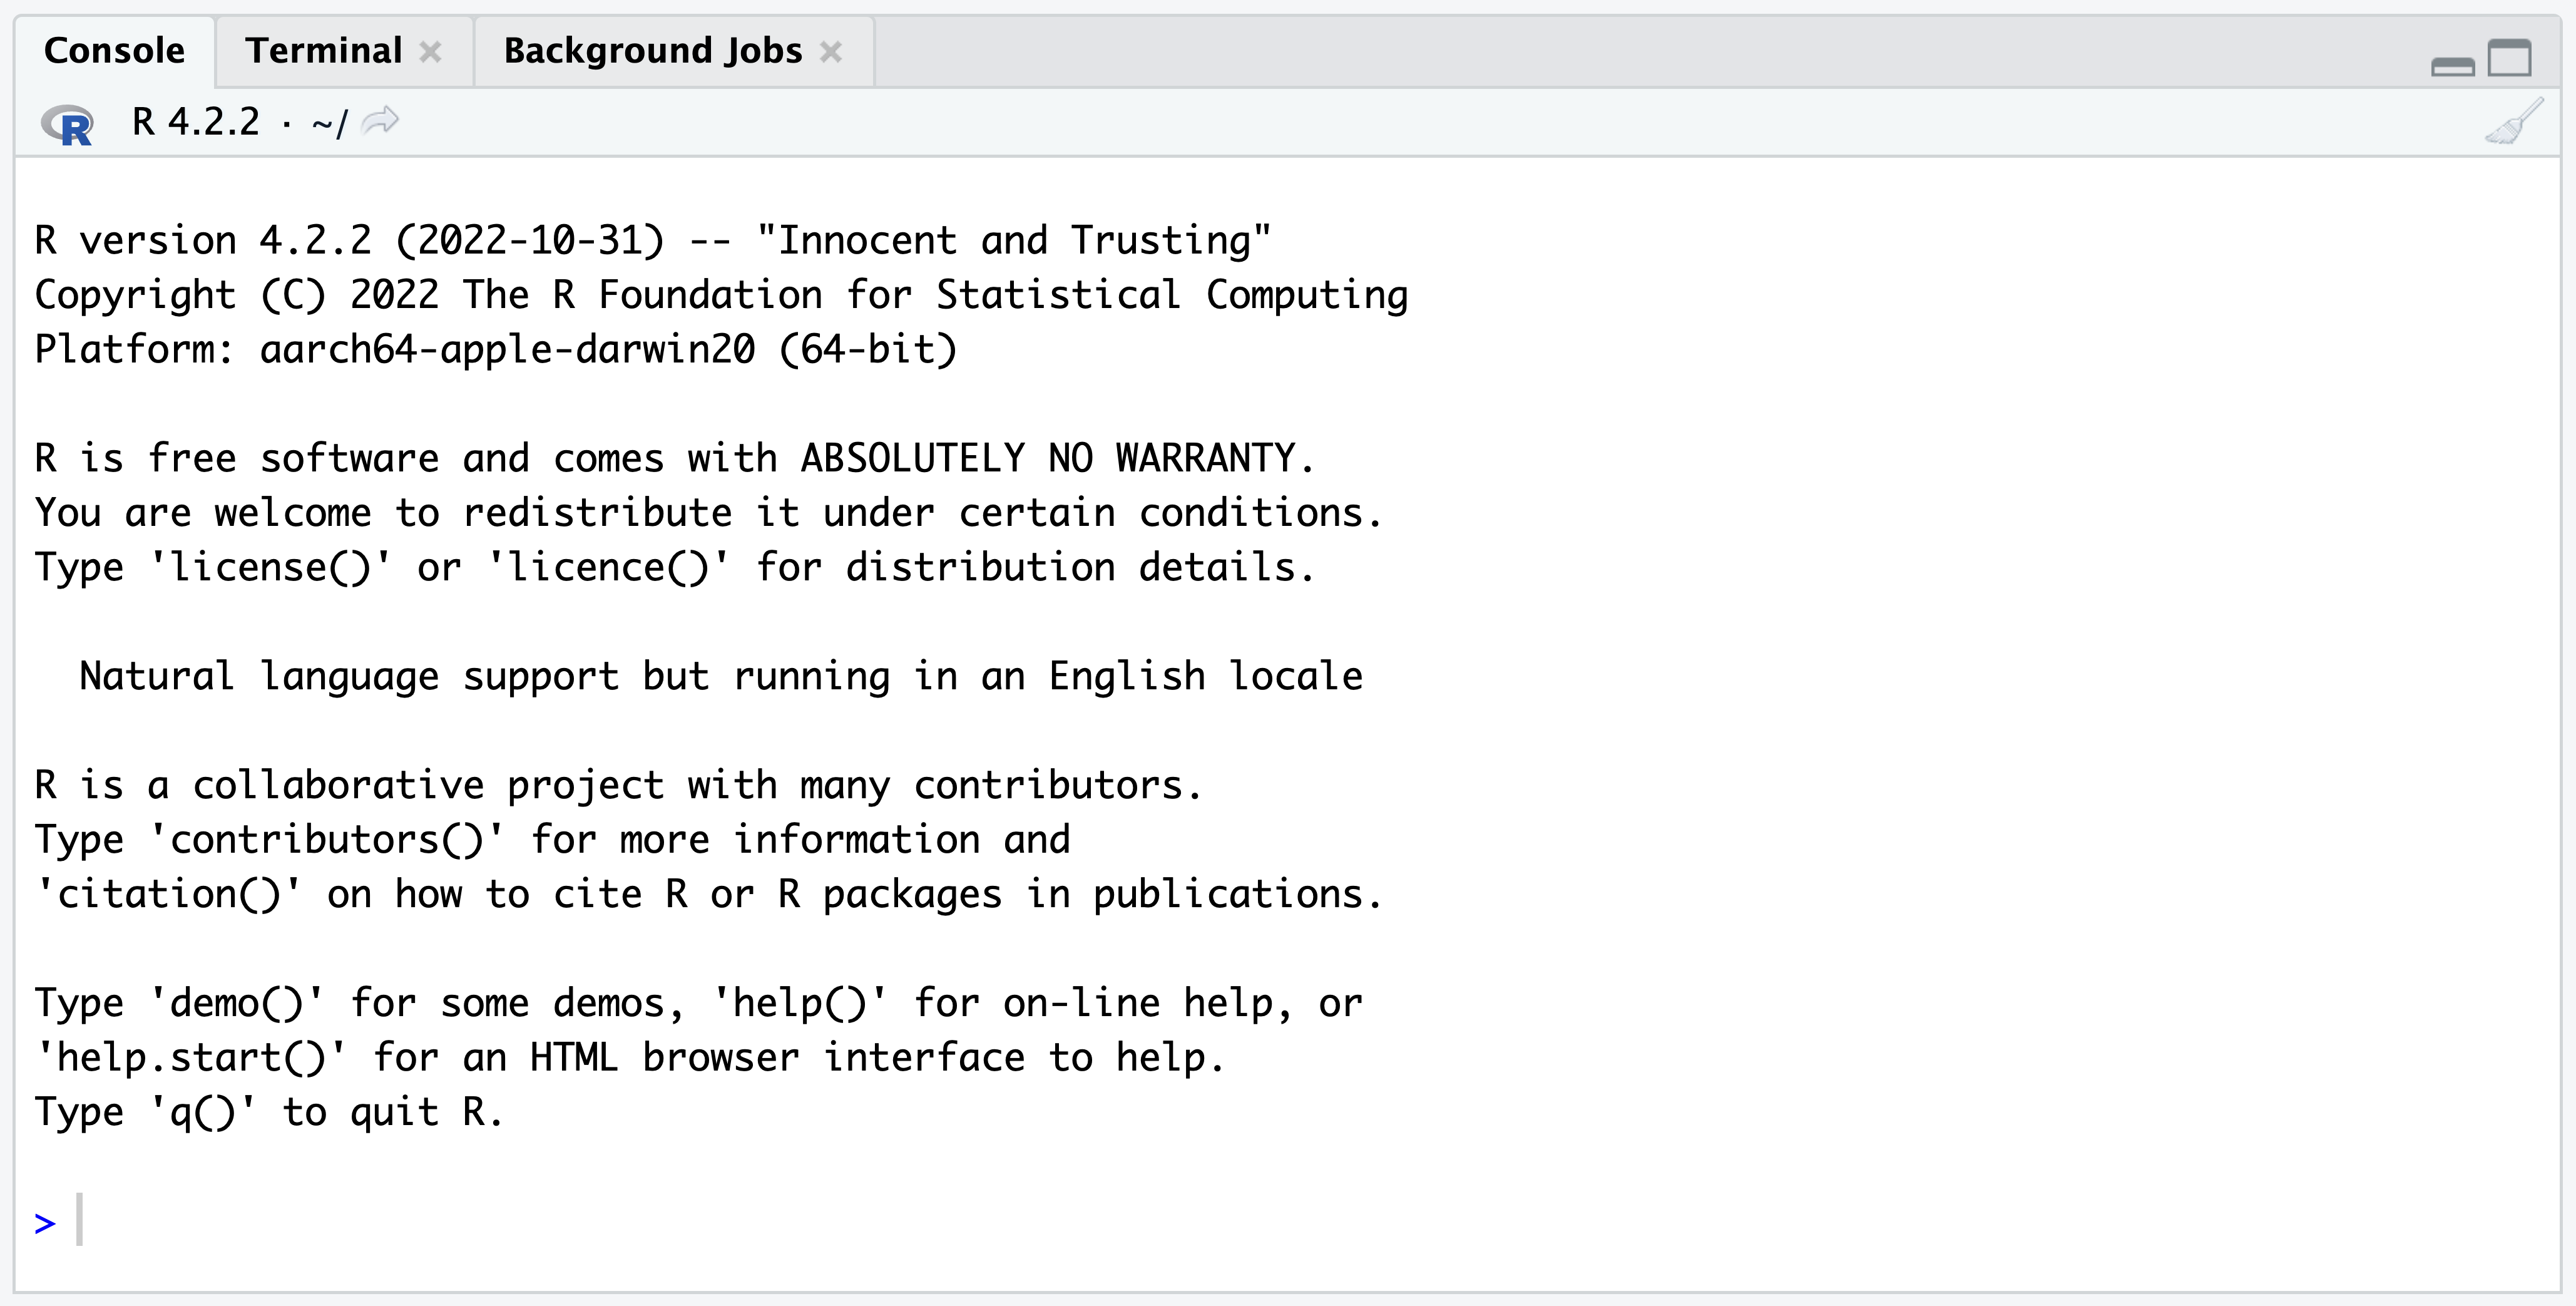
\includegraphics[width=13.72in,height=\textheight]{figures/console.png}

If you click on the console panel (and scroll down to the bottom), you
should see an arrow \texttt{\textgreater{}} with a blinking cursor
\texttt{\textbar{}} symbol. This means that the console is waiting for
you to type your code.

In your console in RStudio, after the \texttt{\textgreater{}} symbol,
type \texttt{2\ +\ 2} and then hit return (Enter).

Your console should have produced the output/result of your code
(\texttt{4}) underneath, and a new arrow \texttt{\textgreater{}} with a
blinking cursor should have appeared underneath, indicating that R is
ready for some more code like this:

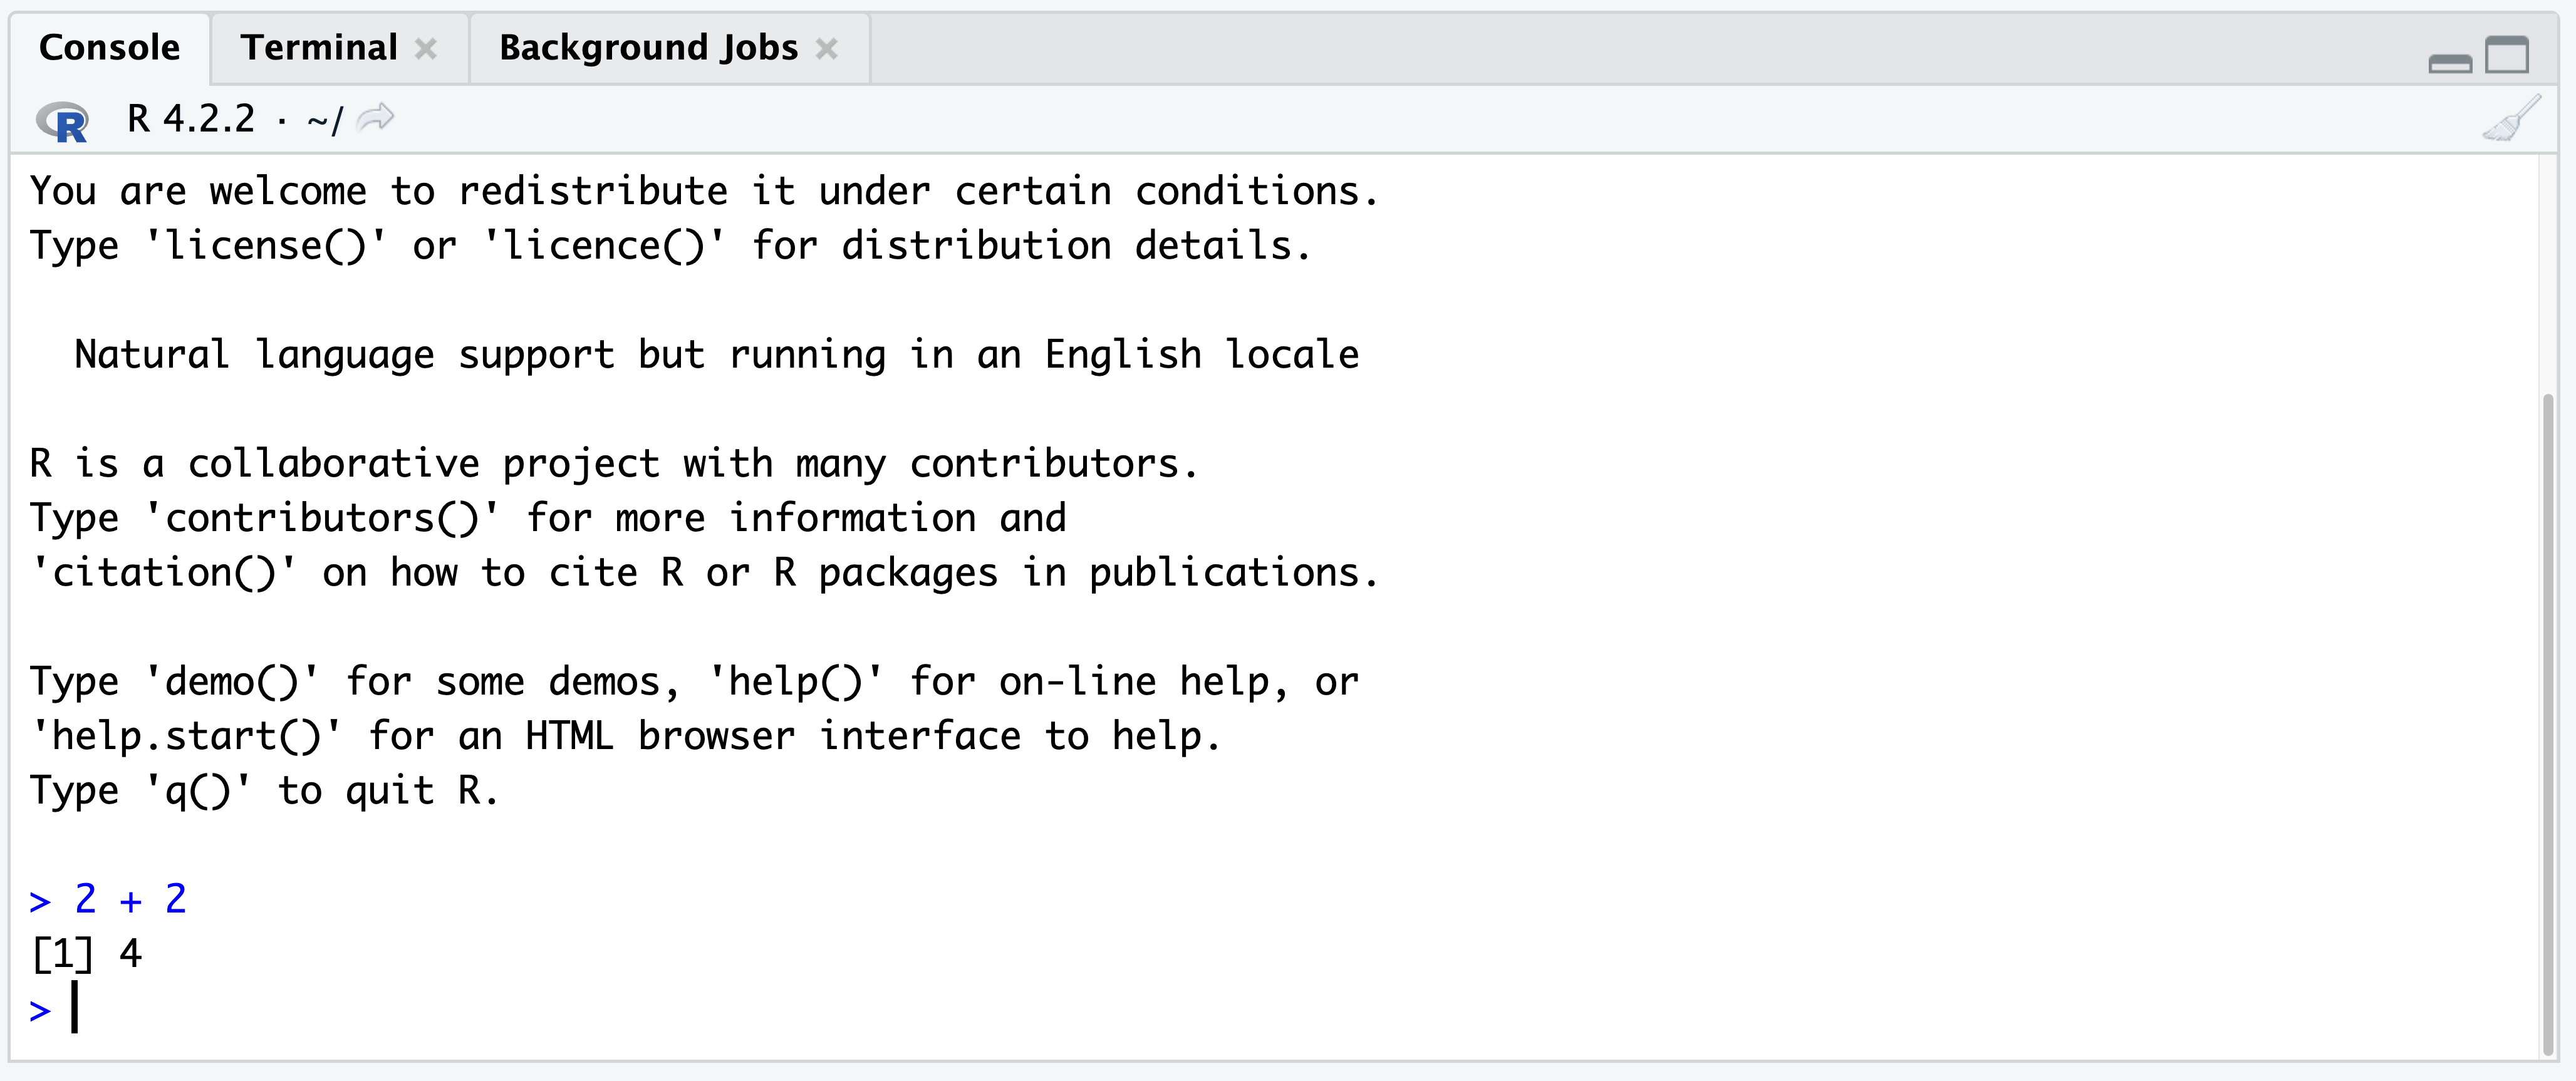
\includegraphics[width=13.71in,height=\textheight]{figures/console_example.png}

So if you can just write your code directly in the console, why bother
with the quarto document at all?

The problem with only ever writing your R code in the R console is that
once you quit RStudio, there will be no record of the code that you ran.

\subsection{Best practices: quarto vs the
console}\label{best-practices-quarto-vs-the-console}

Best practices for writing and saving R code involves writing your code
in R chunks within a quarto document, and then running that code in the
console (and then later rendering your quarto document after you've
written a bunch of code).

This might sound convoluted, but fortunately, you don't have to write
your code in two places. Once you write some code in a code chunk in
your quarto document, you will notice a green ``play'' (right arrow)
button at the right end of the code chunk. If you hit that, you will see
one of two things happen:

\begin{enumerate}
\def\labelenumi{\arabic{enumi}.}
\tightlist
\item
  \textbf{Chunk output inline}: The output of your code will appear
  directly underneath your code chunk \emph{inside} your interactive
  quarto document.
\end{enumerate}

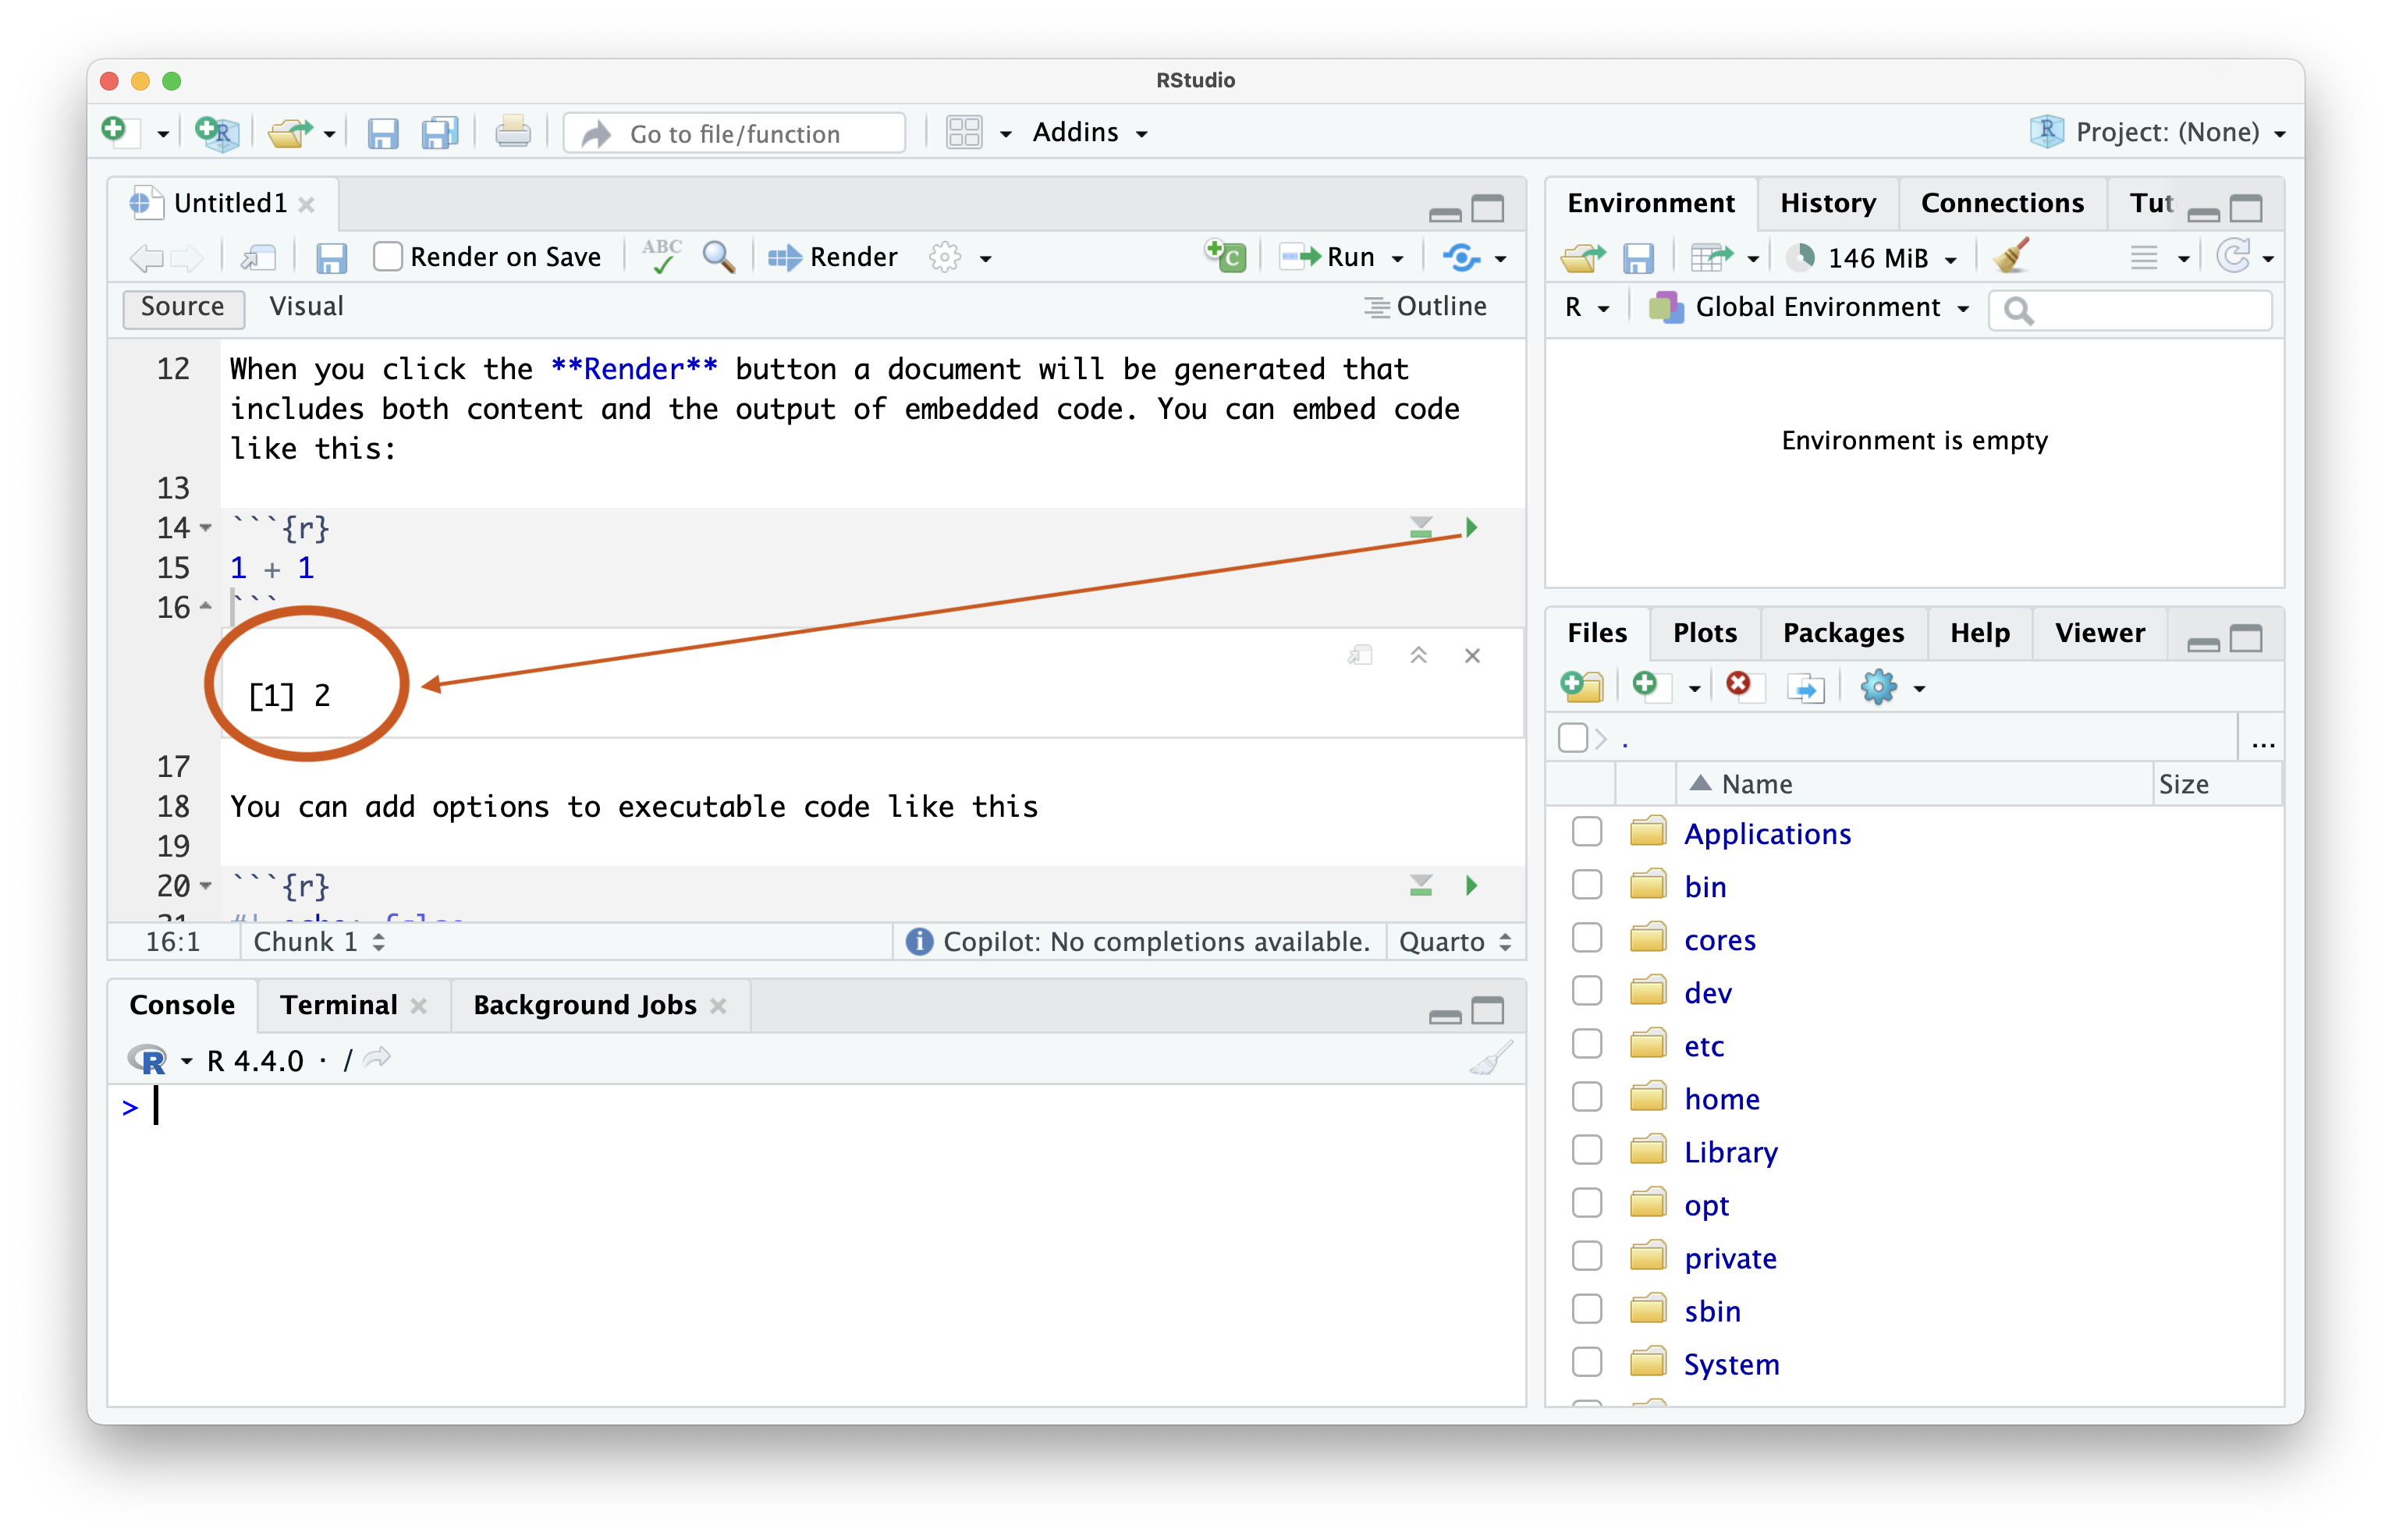
\includegraphics[width=10.22in,height=\textheight]{figures/output_inline.png}

\begin{enumerate}
\def\labelenumi{\arabic{enumi}.}
\setcounter{enumi}{1}
\tightlist
\item
  \textbf{Chunk output in console}: Your code be magically transported
  to the console, where it will be automatically run and the output will
  be shown \emph{in the console}.
\end{enumerate}

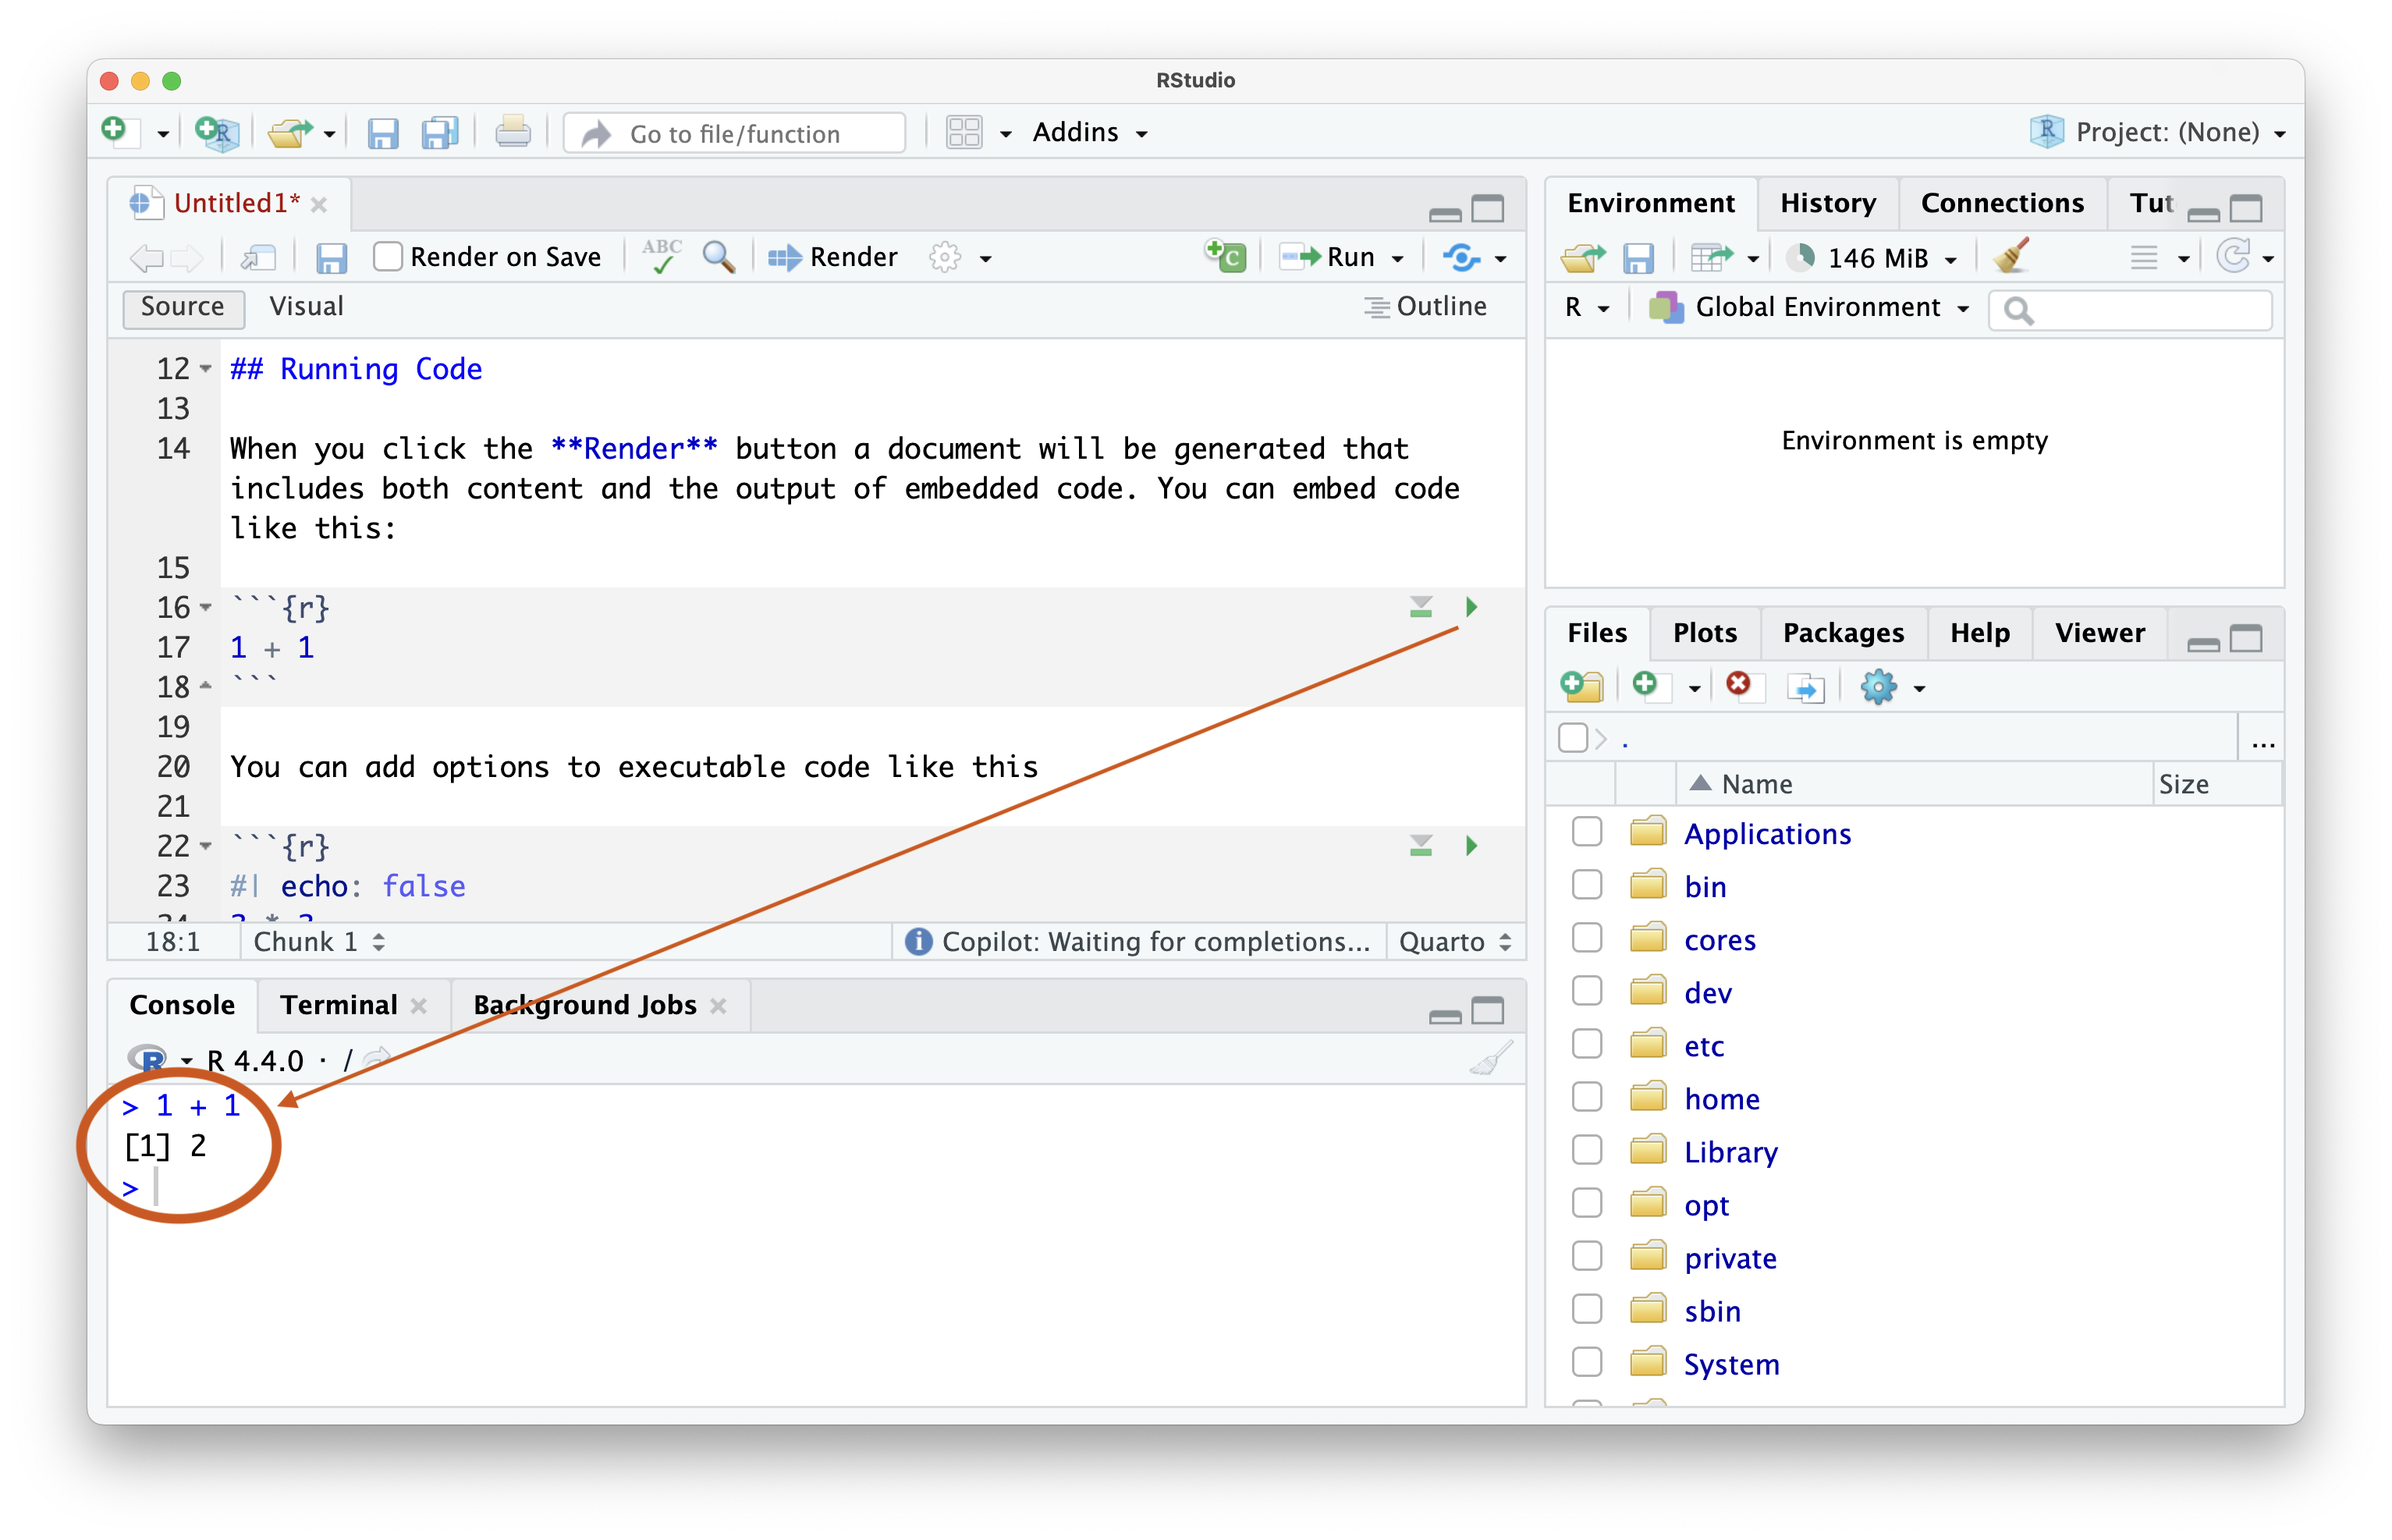
\includegraphics[width=10.22in,height=\textheight]{figures/output_console.png}

\textbf{There is also a nice keyboard shortcut for running the line of
code on which your cursor is: Command+Enter on a Mac or Ctrl+Enter on
Windows and Linux.}

You can change the settings for where your output appears by selecting
the settings button (circled in the image below) and choosing ``Chunk
output inline'' for the first option or ``chunk output in console'' for
the second option.

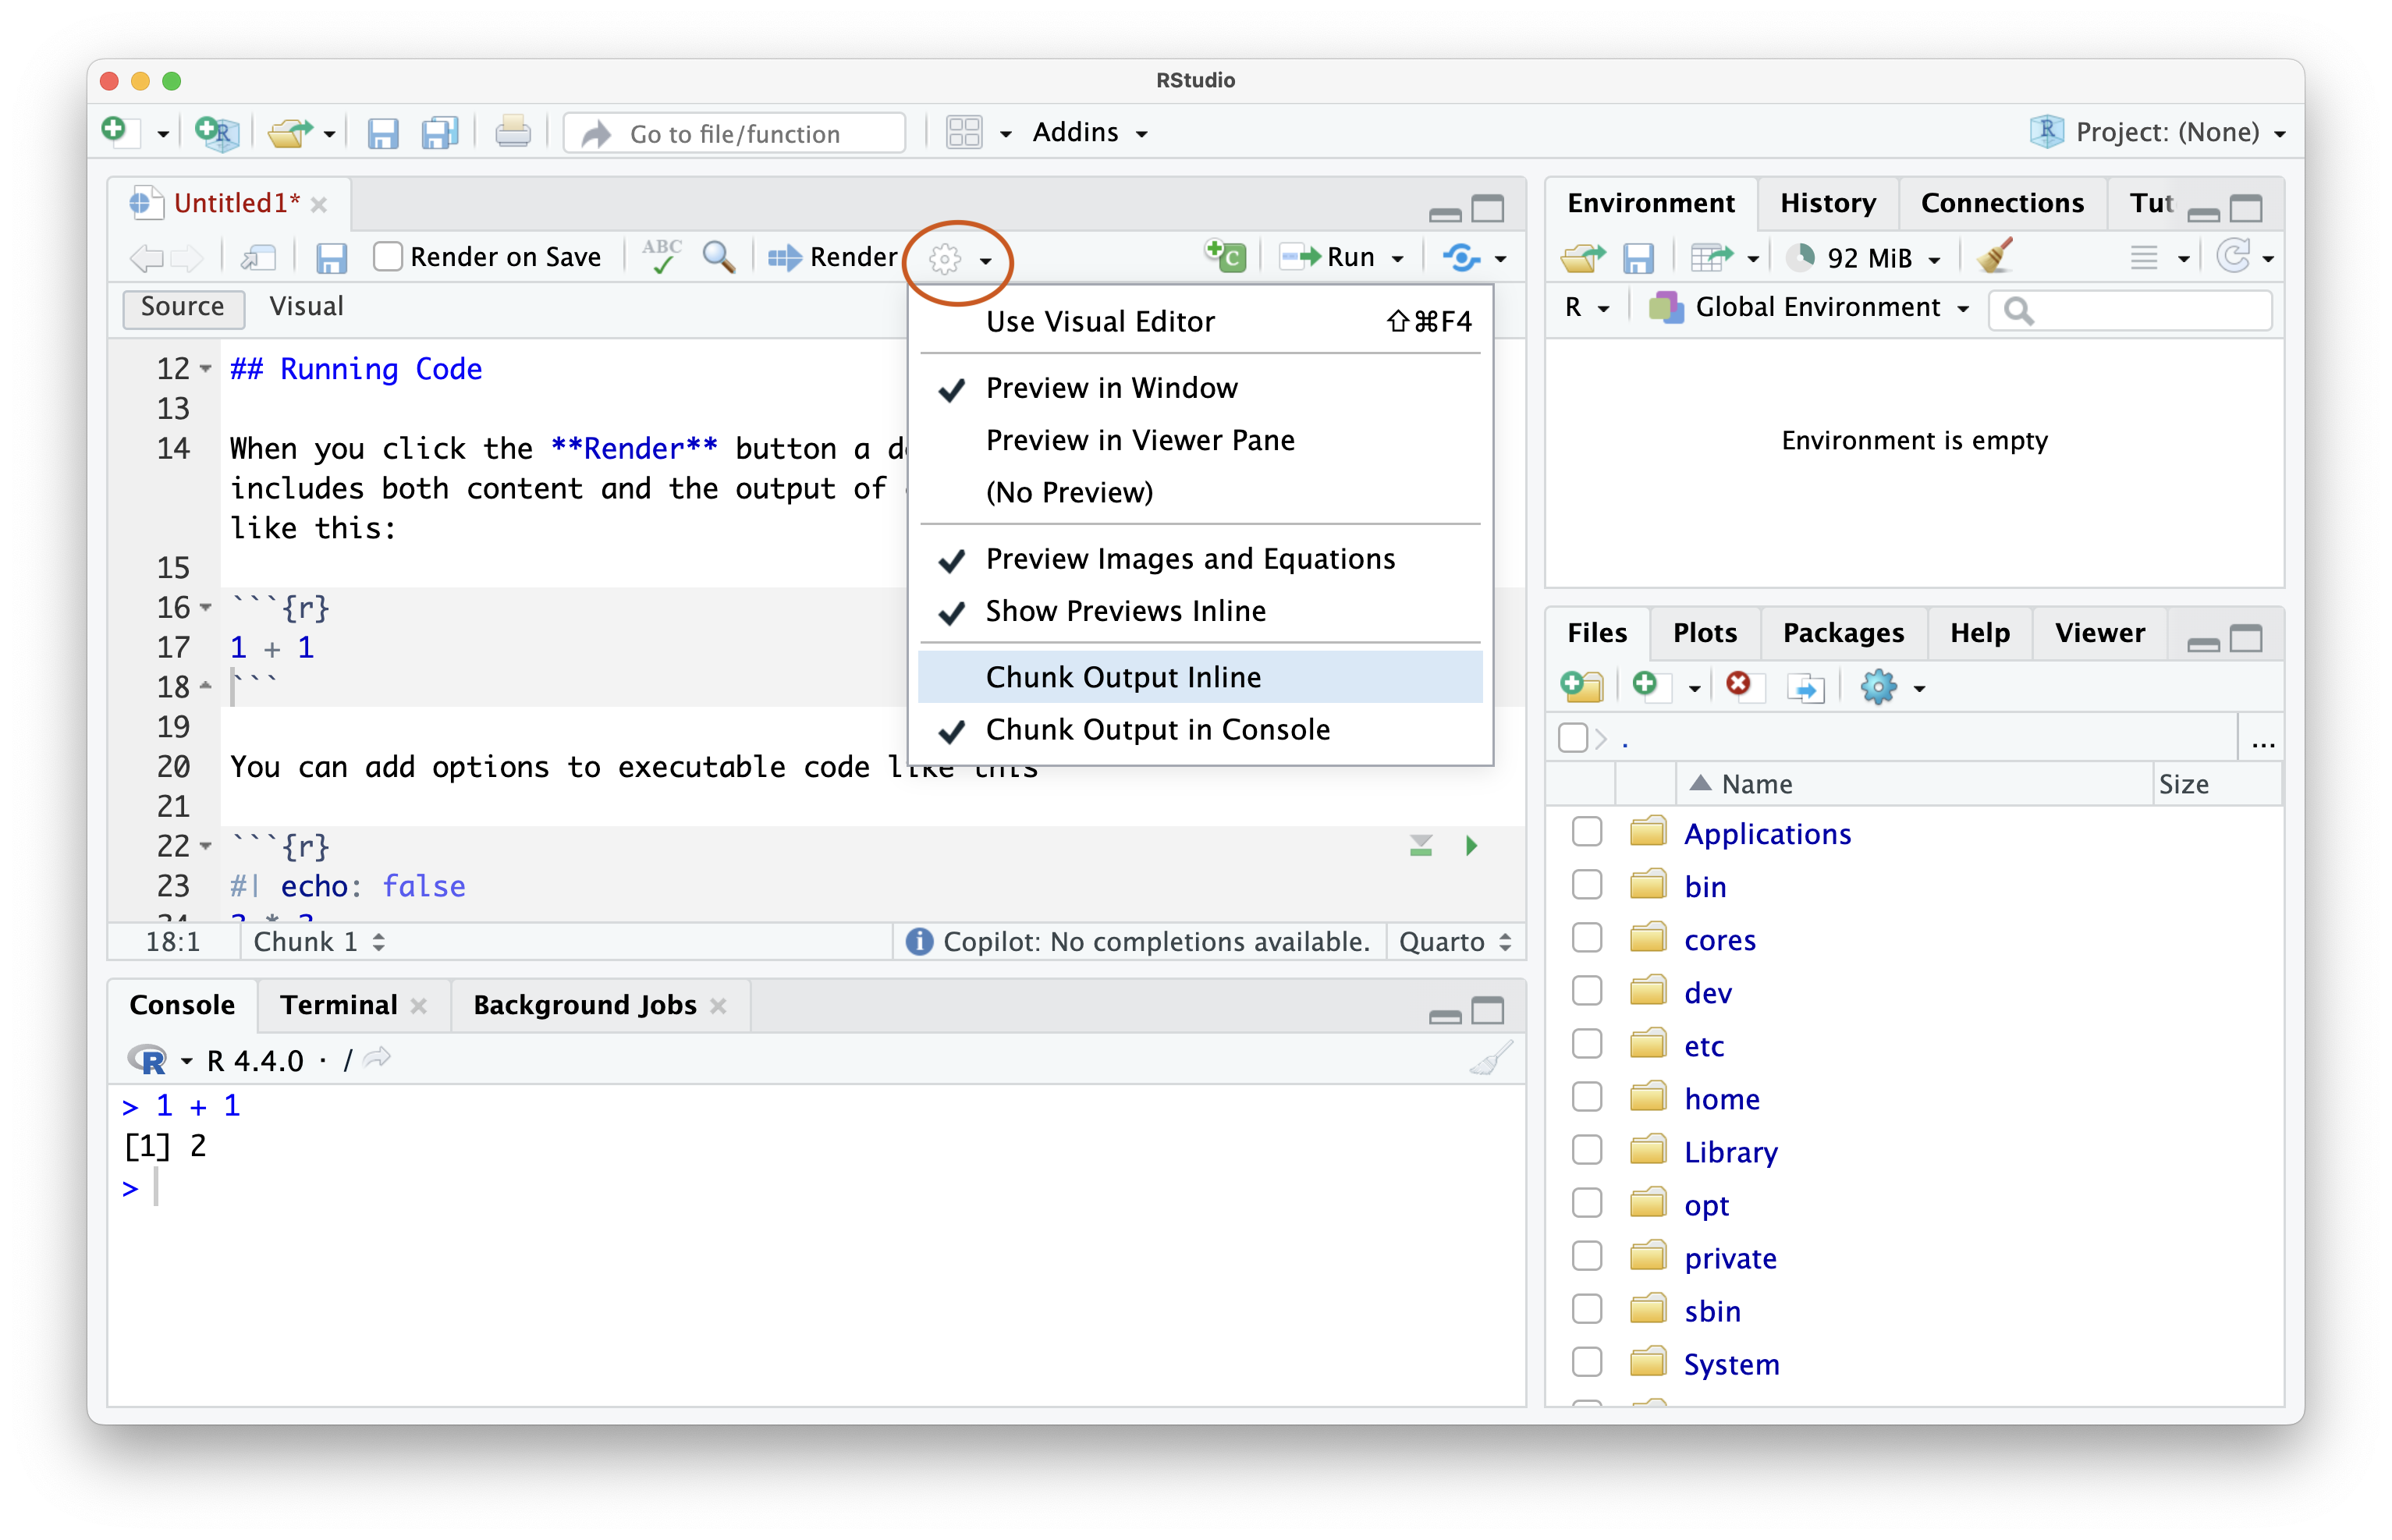
\includegraphics[width=10.22in,height=\textheight]{figures/output_options.png}

I strongly prefer the second option of ``chunk output in console'', but
R users are notoriously divided on where they like their output to
appear (inline or in the console).

My suggestion is try both options for a few hours and see which one
sparks joy.

Regardless of where your output appears (inline or in the console), I
strongly suggest that you write all your code in a quarto document
(rather than directly in the console). Writing your code in a quarto
document will save your code and results in a \emph{reproducible} way
AND help you to communicate your findings to other people.

\subsection{Creating new code chunks in
quarto}\label{creating-new-code-chunks-in-quarto}

In a quarto document you can open a new R code chunk by writing three
backticks followed by the letter ``r'' inside some curly parentheses and
you need to ``close'' the code chunk with three backticks. Anything
between these two lines (inside the grey box) is treated as R code, and
anything outside these two lines is regular text.

\begin{Shaded}
\begin{Highlighting}[]
\InformationTok{\textasciigrave{}\textasciigrave{}\textasciigrave{}\{r\}}


\InformationTok{\textasciigrave{}\textasciigrave{}\textasciigrave{}}
\end{Highlighting}
\end{Shaded}

Since it's a pain to type all that every time you want to create a new
code chunk, you can use one of two shortcuts to create a new code chunk:

\begin{enumerate}
\def\labelenumi{\arabic{enumi}.}
\item
  Hit the ``New Chunk'' button, in RStudio, or
\item
  Use the Option+Command+i keyboard shortcut.
\end{enumerate}

In your quarto document, create three new code chunks, one in each of
the three ways described above. Conduct some basic mathematical
calculations in each code chunk and run the code using any of the
approaches described in the previous section (your output should appear
either inline or in the console, depending on the settings). Then render
your quarto document and look at the html output.

Add a chunk option to hide the code \texttt{\#\textbar{}\ echo:\ false}
to one of your chunks (this echo: false chunk option must go on the
first line of the chunk) and re-run your code (nothing should be
different) and re-render your document and look at the output. What has
changed?

\begin{tcolorbox}[enhanced jigsaw, rightrule=.15mm, toptitle=1mm, title=\textcolor{quarto-callout-warning-color}{\faExclamationTriangle}\hspace{0.5em}{Common issue: I can't find my rendered document}, leftrule=.75mm, bottomtitle=1mm, colbacktitle=quarto-callout-warning-color!10!white, coltitle=black, titlerule=0mm, opacityback=0, colframe=quarto-callout-warning-color-frame, arc=.35mm, opacitybacktitle=0.6, bottomrule=.15mm, left=2mm, breakable, toprule=.15mm, colback=white]

If you can't find your rendered HTML document, find the location where
you saved your quarto document and find the .html file with the same
name. Open this file in your web browser -- this is your rendered
document. If it doesn't update, when you render your quarto document,
there might be an error in your quarto document (check the ``Background
Jobs'' tab in the console panel to see if there are any error messages).

\end{tcolorbox}

\begin{tcolorbox}[enhanced jigsaw, rightrule=.15mm, toptitle=1mm, title=\textcolor{quarto-callout-warning-color}{\faExclamationTriangle}\hspace{0.5em}{Common issue: I can't run my code}, leftrule=.75mm, bottomtitle=1mm, colbacktitle=quarto-callout-warning-color!10!white, coltitle=black, titlerule=0mm, opacityback=0, colframe=quarto-callout-warning-color-frame, arc=.35mm, opacitybacktitle=0.6, bottomrule=.15mm, left=2mm, breakable, toprule=.15mm, colback=white]

R is very particular about the syntax for the code chunks. There must be
no spaces in front of the backticks that define the code chunk and your
chunk options that start with \texttt{\#\textbar{}} must be on the first
line of the code chunk directly under the backticks and not have any
spaces before it.

If your code shortcuts don't work, start super hard at your code chunk
and see if there is anything wrong!

\end{tcolorbox}

\part{R Fundamentals}

\chapter{R Fundamentals}\label{r-fundamentals-1}

\section{Doing math with R}\label{doing-math-with-r}

Who needs a calculator, when you have R! For real though, I legitimately
use R as a basic calculator all the time. And while R can do a lot more
than just compute \texttt{1\ +\ 1}, it's worth taking a moment to
discuss the mathematical capabilities of R.

Here are some helpful math symbols:

\begin{itemize}
\tightlist
\item
  Parentheses: \texttt{(}, \texttt{)}
\item
  Exponents: \texttt{\^{}} or \texttt{**}
\item
  Multiply: \texttt{*}
\item
  Divide: \texttt{/}
\item
  Add: \texttt{+}
\item
  Subtract: \texttt{-}
\end{itemize}

To follow along with the code examples that I provide in this chapter
(and in this book in general), I recommend creating a new quarto
document and practice writing your own code in code chunks in your
quarto document and running the code in the \emph{console} by either
pressing the green play/arrow button in the top right corner of the code
chunks or using the Command+Return shortcut. Feel free to make some of
your own notes in your quarto document outside. I recommend
compiling/rendering your quarto document every now and then too!

Some basic mathematical computations you can compute in R include power
calculations:

\begin{Shaded}
\begin{Highlighting}[]
\NormalTok{(}\DecValTok{3} \SpecialCharTok{+} \DecValTok{5}\NormalTok{)}\SpecialCharTok{\^{}}\DecValTok{2}
\end{Highlighting}
\end{Shaded}

\begin{verbatim}
[1] 64
\end{verbatim}

Division:

\begin{Shaded}
\begin{Highlighting}[]
\DecValTok{2} \SpecialCharTok{/} \DecValTok{7}
\end{Highlighting}
\end{Shaded}

\begin{verbatim}
[1] 0.2857143
\end{verbatim}

Note that R doesn't really care about spaces, so this is the same as

\begin{Shaded}
\begin{Highlighting}[]
\DecValTok{2}\SpecialCharTok{/}\DecValTok{7}
\end{Highlighting}
\end{Shaded}

\begin{verbatim}
[1] 0.2857143
\end{verbatim}

But my recommendation is to always place a single space around
mathematical operators (i.e., \texttt{*}, \texttt{+}, \texttt{-}, etc,
with the exception of the power operator \texttt{\^{}}), so:

\begin{Shaded}
\begin{Highlighting}[]
\DecValTok{2} \SpecialCharTok{+} \DecValTok{1}
\end{Highlighting}
\end{Shaded}

\begin{verbatim}
[1] 3
\end{verbatim}

\begin{Shaded}
\begin{Highlighting}[]
\DecValTok{5} \SpecialCharTok{*} \DecValTok{3}
\end{Highlighting}
\end{Shaded}

\begin{verbatim}
[1] 15
\end{verbatim}

\begin{Shaded}
\begin{Highlighting}[]
\DecValTok{5}\SpecialCharTok{\^{}}\DecValTok{2}
\end{Highlighting}
\end{Shaded}

\begin{verbatim}
[1] 25
\end{verbatim}

When writing code, even if the language itself doesn't require certain
syntax like spaces, it is a good idea to choose a syntax \emph{style}
and stick with it.

You can place multiple computations in the same code chunk, like this:

\begin{Shaded}
\begin{Highlighting}[]
\InformationTok{\textasciigrave{}\textasciigrave{}\textasciigrave{}\{r\}}
\InformationTok{5 + 109}
\InformationTok{(4 + 2) * 4}
\InformationTok{\textasciigrave{}\textasciigrave{}\textasciigrave{}}
\end{Highlighting}
\end{Shaded}

When a code chunk contains multiple pieces of code, they will all be
computed separately when you compile your document and the output will
look like this:

\begin{Shaded}
\begin{Highlighting}[]
\DecValTok{5} \SpecialCharTok{+} \DecValTok{109}
\end{Highlighting}
\end{Shaded}

\begin{verbatim}
[1] 114
\end{verbatim}

\begin{Shaded}
\begin{Highlighting}[]
\NormalTok{(}\DecValTok{4} \SpecialCharTok{+} \DecValTok{2}\NormalTok{) }\SpecialCharTok{*} \DecValTok{4}
\end{Highlighting}
\end{Shaded}

\begin{verbatim}
[1] 24
\end{verbatim}

\section{Code comments}\label{code-comments}

When you have multiple pieces of code in a single code chunk (or even a
single piece of code), it is recommended that you use code comments to
explain what your code is doing. Since R treats everything inside a code
chunk as code, if you want to write some text comments inside a code
chunk, you can tell R that your text is not code by placing a
\texttt{\#} symbol at the beginning of your text like this:

\begin{Shaded}
\begin{Highlighting}[]
\CommentTok{\# compute 4 times 5}
\DecValTok{4} \SpecialCharTok{*} \DecValTok{5}
\end{Highlighting}
\end{Shaded}

\begin{verbatim}
[1] 20
\end{verbatim}

R will ignore anything that follows a \texttt{\#} symbol. So in the
above code chunk, R will ignore the first line with the code comment
``compute 4 times 5'', and then it will compute the R code on the next
line, \texttt{4\ *\ 5}.

Code comments are really helpful for explaining what your code is doing.
I usually reserve the text outside code chunks for more general
discussion of my data, analysis, and results and I reserve code comments
inside code chunks for explaining my code itself. I tend to forget the
reasons behind certain decisions I made in my code, but adding
explanations in code comments helps me remember my motivations and
intentions days, months, or even years later.

\section{Scientific notation}\label{scientific-notation}

When doing mathematical calculations in R, very quickly you are going to
start encountering some very strange looking output. For example, if I
compute

\begin{Shaded}
\begin{Highlighting}[]
\DecValTok{1} \SpecialCharTok{/} \DecValTok{70000}
\end{Highlighting}
\end{Shaded}

\begin{verbatim}
[1] 1.428571e-05
\end{verbatim}

or

\begin{Shaded}
\begin{Highlighting}[]
\DecValTok{12}\SpecialCharTok{\^{}}\DecValTok{15}
\end{Highlighting}
\end{Shaded}

\begin{verbatim}
[1] 1.540702e+16
\end{verbatim}

You can see that my output looks a little strange.

When a number is very big or very small, R gets lazy and decides that it
doesn't want to print all of its digits. Rather than just making up
random numbers, R is printing these numbers in scientific notation.
\texttt{2e-05} means ``0.00002'', i.e., there is a 2 in the 5th decimal
place. On the other hand, \texttt{2e+05} (with a \texttt{+} instead of
\texttt{-}), corresponds to 200000, i.e., ``2'' with 5 0's after it.

\begin{tcolorbox}[enhanced jigsaw, rightrule=.15mm, toptitle=1mm, title=\textcolor{quarto-callout-tip-color}{\faLightbulb}\hspace{0.5em}{No commas allowed!}, leftrule=.75mm, bottomtitle=1mm, colbacktitle=quarto-callout-tip-color!10!white, coltitle=black, titlerule=0mm, opacityback=0, colframe=quarto-callout-tip-color-frame, arc=.35mm, opacitybacktitle=0.6, bottomrule=.15mm, left=2mm, breakable, toprule=.15mm, colback=white]

Note that R doesn't allow for commas in numbers. If you want to write a
large number, you have to remove the comma:

\begin{Shaded}
\begin{Highlighting}[]
\CommentTok{\# this is fine}
\DecValTok{70000}
\end{Highlighting}
\end{Shaded}

\begin{verbatim}
[1] 70000
\end{verbatim}

\begin{Shaded}
\begin{Highlighting}[]
\CommentTok{\# this is not fine {-}{-} note the "error" message}
\DecValTok{70}\NormalTok{,}\DecValTok{000}
\end{Highlighting}
\end{Shaded}

\begin{verbatim}
Error: <text>:1:3: unexpected ','
1: 70,
      ^
\end{verbatim}

\end{tcolorbox}

\section{Mathematical functions}\label{mathematical-functions}

While being able to do addition, subtraction, and multiplication is
super awesome, sometimes you will need to use more complex mathematical
operations in your computations, such as the logarithm, exponential, and
square-root. Fortunately there are \textbf{functions} in R that let you
compute these operations.

A function is a piece of R code that is referenced using alias or a
name. A function typically takes an ``argument'', such as a number, and
it does something to the argument, such as compute the logarithm, and
then it returns the result.

To apply a function to a value, you write the name of the function
(e.g., \texttt{log}), followed by some parentheses \texttt{()}, inside
which you provide the argument or value that you want to apply the
function to, as in: \texttt{log(2)}.

\begin{Shaded}
\begin{Highlighting}[]
\CommentTok{\# compute the square root of 2}
\FunctionTok{sqrt}\NormalTok{(}\DecValTok{2}\NormalTok{)}
\end{Highlighting}
\end{Shaded}

\begin{verbatim}
[1] 1.414214
\end{verbatim}

\begin{Shaded}
\begin{Highlighting}[]
\CommentTok{\# compute the log of 2}
\FunctionTok{log}\NormalTok{(}\DecValTok{2}\NormalTok{)}
\end{Highlighting}
\end{Shaded}

\begin{verbatim}
[1] 0.6931472
\end{verbatim}

\begin{Shaded}
\begin{Highlighting}[]
\CommentTok{\# compute e\^{}2}
\FunctionTok{exp}\NormalTok{(}\DecValTok{2}\NormalTok{)}
\end{Highlighting}
\end{Shaded}

\begin{verbatim}
[1] 7.389056
\end{verbatim}

\section{Defining variables}\label{defining-variables}

One of the main features of coding in R is defining ``objects'' or
``variables'' (I use these terms interchangeably). Creating a variable
essentially involves giving a value a name, allowing you to reference
that value later. When we are ready to load some actual data, we will
give that data a name by storing it in a variable.

Let's store the value \texttt{1} in a variable called
\texttt{my\_variable} using the \textbf{assignment operator}:
\texttt{my\_variable\ \textless{}-\ 1}. Think of the assignment operator
\texttt{\textless{}-} as an arrow, pointing from the value on the right
to the variable name on the left.

\begin{Shaded}
\begin{Highlighting}[]
\NormalTok{my\_variable }\OtherTok{\textless{}{-}} \DecValTok{1} 
\end{Highlighting}
\end{Shaded}

Note that when you define a variable, no output is shown.

You can view the value of \texttt{my\_variable} by writing it's name:

\begin{Shaded}
\begin{Highlighting}[]
\NormalTok{my\_variable}
\end{Highlighting}
\end{Shaded}

\begin{verbatim}
[1] 1
\end{verbatim}

You can think of \texttt{my\_variable} as an alias for the value
\texttt{1}. This means that anything that I could do to the value
\texttt{1}, I can now do to \texttt{my\_variable}, such as adding
\texttt{2} to it:

\begin{Shaded}
\begin{Highlighting}[]
\NormalTok{my\_variable }\SpecialCharTok{+} \DecValTok{2}
\end{Highlighting}
\end{Shaded}

\begin{verbatim}
[1] 3
\end{verbatim}

\begin{tcolorbox}[enhanced jigsaw, rightrule=.15mm, toptitle=1mm, title=\textcolor{quarto-callout-tip-color}{\faLightbulb}\hspace{0.5em}{R is case sensitive}, leftrule=.75mm, bottomtitle=1mm, colbacktitle=quarto-callout-tip-color!10!white, coltitle=black, titlerule=0mm, opacityback=0, colframe=quarto-callout-tip-color-frame, arc=.35mm, opacitybacktitle=0.6, bottomrule=.15mm, left=2mm, breakable, toprule=.15mm, colback=white]

R is case sensitive, which means that I must write my variable name
exactly as it is written. For example, the following will yield an
error:

\begin{Shaded}
\begin{Highlighting}[]
\NormalTok{my\_Variable}
\end{Highlighting}
\end{Shaded}

\begin{verbatim}
Error in eval(expr, envir, enclos): object 'my_Variable' not found
\end{verbatim}

because the variable is called \texttt{my\_variable}, not
\texttt{my\_Variable}.

\end{tcolorbox}

\begin{tcolorbox}[enhanced jigsaw, rightrule=.15mm, toptitle=1mm, title=\textcolor{quarto-callout-tip-color}{\faLightbulb}\hspace{0.5em}{Defining variables using \texttt{=}}, leftrule=.75mm, bottomtitle=1mm, colbacktitle=quarto-callout-tip-color!10!white, coltitle=black, titlerule=0mm, opacityback=0, colframe=quarto-callout-tip-color-frame, arc=.35mm, opacitybacktitle=0.6, bottomrule=.15mm, left=2mm, breakable, toprule=.15mm, colback=white]

Another way to define a variable is using ``=''.

Below, I create \texttt{another\_variable}, assign it the value
\texttt{3}

\begin{Shaded}
\begin{Highlighting}[]
\NormalTok{another\_variable }\OtherTok{=} \DecValTok{3}
\NormalTok{another\_variable }
\end{Highlighting}
\end{Shaded}

\begin{verbatim}
[1] 3
\end{verbatim}

But convention in the R community prefers the use of the
\texttt{\textless{}-} assignment operator over the \texttt{=} assignment
operator. So while, \texttt{=} will work just fine, it is a lot less
common among seasoned R programmers.

\end{tcolorbox}

Whenever we do a mathematical calculations using numeric values, we
create a new numeric value, for example, the computation

\begin{Shaded}
\begin{Highlighting}[]
\DecValTok{1} \SpecialCharTok{+} \DecValTok{1}
\end{Highlighting}
\end{Shaded}

\begin{verbatim}
[1] 2
\end{verbatim}

creates the value \texttt{2}.

You can also assign the \emph{output} of mathematical calculations to a
variable.

\begin{Shaded}
\begin{Highlighting}[]
\CommentTok{\# assign the output of 1 + 1 to the variable one\_plus\_one}
\NormalTok{one\_plus\_one }\OtherTok{\textless{}{-}} \DecValTok{1} \SpecialCharTok{+} \DecValTok{1}
\NormalTok{one\_plus\_one}
\end{Highlighting}
\end{Shaded}

\begin{verbatim}
[1] 2
\end{verbatim}

It is important to make the distinction that \texttt{one\_plus\_one}
does not contain the mathematical \emph{equation} \texttt{1\ +\ 1}.
Instead, it contains the numerical value, \texttt{2}, which is the
\emph{output} of the equation \texttt{1\ +\ 1}.

\texttt{one\_plus\_one} doesn't remember that it was created by
computing \texttt{1\ +\ 1}, it just knows that the value it contains is
\texttt{2}.

\section{Exercise}

Define a new object \texttt{prod} that contains the output of the
product of 5 and 2. Print out \texttt{prod} by writing its name

\section{Solution}

\begin{Shaded}
\begin{Highlighting}[]
\NormalTok{prod }\OtherTok{\textless{}{-}} \DecValTok{5} \SpecialCharTok{*} \DecValTok{2}
\NormalTok{prod}
\end{Highlighting}
\end{Shaded}

\begin{verbatim}
[1] 10
\end{verbatim}

\subsection{Overwriting variables}\label{overwriting-variables}

Below I define \texttt{my\_number} to be a variable containing the
numeric value \texttt{5}.

\begin{Shaded}
\begin{Highlighting}[]
\NormalTok{my\_number }\OtherTok{\textless{}{-}} \DecValTok{5}
\end{Highlighting}
\end{Shaded}

Next, I define a new variable called \texttt{result}, that contains the
product of \texttt{my\_number} and \texttt{7}, and I print it out:

\begin{Shaded}
\begin{Highlighting}[]
\NormalTok{result }\OtherTok{\textless{}{-}}\NormalTok{ my\_number }\SpecialCharTok{*} \DecValTok{7}
\NormalTok{result}
\end{Highlighting}
\end{Shaded}

\begin{verbatim}
[1] 35
\end{verbatim}

Here, \texttt{result} is defined based on the value of
\texttt{my\_number}.

What do you think would happen to \texttt{result} if I redefine
\texttt{my\_number} to now contain \texttt{8}?

\begin{Shaded}
\begin{Highlighting}[]
\CommentTok{\# update the value of my\_number to be 8}
\NormalTok{my\_number }\OtherTok{\textless{}{-}} \DecValTok{8}
\end{Highlighting}
\end{Shaded}

Do you think \texttt{result} will have changed? Try it yourself in
RStudio or click the ``Answer'' tab below.

\section{Question}

What happens to \texttt{result}?

\section{Answer}

\begin{Shaded}
\begin{Highlighting}[]
\CommentTok{\# define result using \textasciigrave{}my\_number\textasciigrave{}}
\NormalTok{result }\OtherTok{\textless{}{-}}\NormalTok{ my\_number }\SpecialCharTok{*} \DecValTok{7}
\NormalTok{result}
\end{Highlighting}
\end{Shaded}

\begin{verbatim}
[1] 56
\end{verbatim}

\begin{Shaded}
\begin{Highlighting}[]
\CommentTok{\# modify my\_number}
\NormalTok{my\_number }\OtherTok{\textless{}{-}} \DecValTok{8}
\end{Highlighting}
\end{Shaded}

Result does not change.

\begin{Shaded}
\begin{Highlighting}[]
\NormalTok{result}
\end{Highlighting}
\end{Shaded}

\begin{verbatim}
[1] 56
\end{verbatim}

When we defined \texttt{result\ \textless{}-\ my\_number\ *\ 7}, we
assigned result to the \emph{output} of \texttt{my\_number\ *\ 7}, which
is \texttt{56}.

Once it has been defined, \texttt{result} forgets all about
\texttt{my\_number}, it just remembers the value \texttt{56}.

This means that changing \texttt{my\_number} \emph{after} having defined
\texttt{result} will have no effect on \texttt{result}. There is no link
between the two variables, despite the fact that \texttt{result} was
originally defined using \texttt{my\_number}!

\section{Exercise}

Without running the code below, guess what the output/result will be:

\begin{Shaded}
\begin{Highlighting}[]
\NormalTok{value }\OtherTok{\textless{}{-}} \DecValTok{1}
\NormalTok{computed\_result }\OtherTok{\textless{}{-}}\NormalTok{ value }\SpecialCharTok{*} \DecValTok{10} \SpecialCharTok{+} \DecValTok{3}\SpecialCharTok{\^{}}\DecValTok{2}
\NormalTok{value }\OtherTok{\textless{}{-}}\NormalTok{ value }\SpecialCharTok{+} \DecValTok{2}
\NormalTok{computed\_result }
\end{Highlighting}
\end{Shaded}

\section{Solution}

Note that the first three lines of code all involve defining variables
and so no output is shown when these are run. The final line of code
will print out the value of \texttt{computed\_result}.

The second line
\texttt{computed\_result\ \textless{}-\ value\ *\ 10\ +\ 3\^{}2} defines
\texttt{computed\_result} using \texttt{value}. Then the third line
\texttt{value\ \textless{}-\ value\ +\ 2} updates value. Since
\texttt{computed\_result} is assigned to the \emph{output} of
\texttt{value\ *\ 10\ +\ 3\^{}2}, which is \texttt{19}, it doesn't care
when \texttt{value} is subsequently updated, and so the
\texttt{computed\_result} is still just equal to \texttt{19}:

\begin{Shaded}
\begin{Highlighting}[]
\NormalTok{value }\OtherTok{\textless{}{-}} \DecValTok{1}
\NormalTok{computed\_result }\OtherTok{\textless{}{-}}\NormalTok{ value }\SpecialCharTok{*} \DecValTok{10} \SpecialCharTok{+} \DecValTok{3}\SpecialCharTok{\^{}}\DecValTok{2}
\NormalTok{value }\OtherTok{\textless{}{-}}\NormalTok{ value }\SpecialCharTok{+} \DecValTok{2}
\NormalTok{computed\_result }
\end{Highlighting}
\end{Shaded}

\begin{verbatim}
[1] 19
\end{verbatim}

\subsection{Variable names}\label{variable-names}

While you can give your variables \emph{almost} any name you like, there
are a few rules that you need follow.

While variable names can contain letters, numbers, underscores, and
periods, recommended convention specifies that variable names should
contain purely \textbf{lowercase letters and numbers, with words
separated by underscores}.

For example, \texttt{var\_name} and \texttt{my\_var} are considered
``good'' variable names, whereas \texttt{varName}, \texttt{VarName}, and
\texttt{var.name} are not.

Note that variable names cannot \emph{begin} with numbers or
underscores. If you try to create variables whose names are illegal, you
will get an error, such as:

\begin{Shaded}
\begin{Highlighting}[]
\DecValTok{1}\NormalTok{plus1 }\OtherTok{\textless{}{-}} \DecValTok{1} \SpecialCharTok{+} \DecValTok{1}
\end{Highlighting}
\end{Shaded}

\begin{verbatim}
Error: <text>:1:2: unexpected symbol
1: 1plus1
     ^
\end{verbatim}

\begin{Shaded}
\begin{Highlighting}[]
\NormalTok{\_var }\OtherTok{\textless{}{-}} \DecValTok{1} \SpecialCharTok{+} \DecValTok{1}
\end{Highlighting}
\end{Shaded}

\begin{verbatim}
Error: <text>:1:2: unexpected symbol
1: _var
     ^
\end{verbatim}

\section{Exercise}

Which of the following are valid R variable names? Which ones are
\emph{good} variable names?

\begin{Shaded}
\begin{Highlighting}[]
\NormalTok{min\_height}
\NormalTok{max.height}
\NormalTok{\_age}
\NormalTok{MaxLength}
\NormalTok{min}\SpecialCharTok{{-}}\NormalTok{length}
\DecValTok{2}\NormalTok{widths}
\end{Highlighting}
\end{Shaded}

\section{Solution}

\begin{itemize}
\item
  \texttt{min\_height}: this is a \textbf{good} variable name
\item
  \texttt{max.height}: this is a \textbf{valid} variable name, but not
  necessarily a ``good'' variable name (words should be separated with
  \texttt{\_}, not \texttt{.})
\item
  \texttt{\_age}: this is \textbf{not a valid} variable name (variable
  names cannot start with \texttt{\_})
\item
  \texttt{MaxLength}: this is a \textbf{valid} variable name, but not
  necessarily a ``good'' variable name (words should be lowercase and
  separated with underscores)
\item
  \texttt{min-length}: this is \textbf{not a valid} variable name (words
  should be separated with \texttt{\_}, not the minus sign \texttt{-})
\item
  \texttt{2widths}: this is \textbf{not a valid} variable name (variable
  names cannot start with numbers)
\end{itemize}

\chapter{Types}\label{types}

\section{Common object types}\label{common-object-types}

So far, we have only worked with numbers in R. But there are many other
kinds of values that you will encounter in your R journeys.

The main types of values that you'll encounter in R are:

\begin{itemize}
\item
  \textbf{Numeric}: numbers, e.g., \texttt{1}, \texttt{3.5},
  \texttt{1e5} (which is scientific notation for 100,000)
\item
  \textbf{Character}: free-form text values, e.g.,
  \texttt{"California"}, \texttt{"John\ Doe"}, \texttt{"XJ1784"}
\item
  \textbf{Logical} (Boolean): binary values corresponding to
  \texttt{TRUE} and \texttt{FALSE}
\end{itemize}

\subsection{Numeric values}\label{numeric-values}

You can use the \texttt{class()} function to ask what type of object a
value is. For example, the class of \texttt{9.6} is ``numeric''

\begin{Shaded}
\begin{Highlighting}[]
\FunctionTok{class}\NormalTok{(}\FloatTok{9.6}\NormalTok{)}
\end{Highlighting}
\end{Shaded}

\begin{verbatim}
[1] "numeric"
\end{verbatim}

So is the class of \texttt{-5}

\begin{Shaded}
\begin{Highlighting}[]
\FunctionTok{class}\NormalTok{(}\SpecialCharTok{{-}}\DecValTok{5}\NormalTok{)}
\end{Highlighting}
\end{Shaded}

\begin{verbatim}
[1] "numeric"
\end{verbatim}

and \texttt{1e7} (which is scientific notation for 10,000,000)

\begin{Shaded}
\begin{Highlighting}[]
\FunctionTok{class}\NormalTok{(}\FloatTok{1e7}\NormalTok{)}
\end{Highlighting}
\end{Shaded}

\begin{verbatim}
[1] "numeric"
\end{verbatim}

You can also use the \texttt{class()} function to ask the class of the
value stored in a \emph{variable}:

\begin{Shaded}
\begin{Highlighting}[]
\NormalTok{y }\OtherTok{\textless{}{-}} \DecValTok{2} \SpecialCharTok{*} \DecValTok{3} \SpecialCharTok{+} \DecValTok{1}
\NormalTok{y}
\end{Highlighting}
\end{Shaded}

\begin{verbatim}
[1] 7
\end{verbatim}

Identify the class of \texttt{y} (which contains the value \texttt{7}):

\begin{Shaded}
\begin{Highlighting}[]
\FunctionTok{class}\NormalTok{(y)}
\end{Highlighting}
\end{Shaded}

\begin{verbatim}
[1] "numeric"
\end{verbatim}

If your object has class \texttt{"numeric"}, you can do mathematical
computations with it:

\begin{Shaded}
\begin{Highlighting}[]
\NormalTok{y }\SpecialCharTok{+} \DecValTok{2}
\end{Highlighting}
\end{Shaded}

\begin{verbatim}
[1] 9
\end{verbatim}

\begin{Shaded}
\begin{Highlighting}[]
\NormalTok{y}\SpecialCharTok{\^{}}\DecValTok{3}
\end{Highlighting}
\end{Shaded}

\begin{verbatim}
[1] 343
\end{verbatim}

\section{Exercise}

Identify the class (type) of the value \texttt{99.9}

\section{Solution}

\begin{Shaded}
\begin{Highlighting}[]
\FunctionTok{class}\NormalTok{(}\FloatTok{99.9}\NormalTok{)}
\end{Highlighting}
\end{Shaded}

\begin{verbatim}
[1] "numeric"
\end{verbatim}

\subsection{Character values}\label{character-values}

Many datasets will contain text as well as numbers! In R, text has a
``character'' type.

The following contain examples of character type values:

\begin{Shaded}
\begin{Highlighting}[]
\StringTok{"banana"}
\end{Highlighting}
\end{Shaded}

\begin{verbatim}
[1] "banana"
\end{verbatim}

\begin{Shaded}
\begin{Highlighting}[]
\StringTok{"I really like owls"}
\end{Highlighting}
\end{Shaded}

\begin{verbatim}
[1] "I really like owls"
\end{verbatim}

And like numbers, you can save character type values in a variable:

\begin{Shaded}
\begin{Highlighting}[]
\NormalTok{char\_var }\OtherTok{\textless{}{-}} \StringTok{"my first character variable"}
\end{Highlighting}
\end{Shaded}

And to view the contents of our character variable, you just type its
name as usual:

\begin{Shaded}
\begin{Highlighting}[]
\NormalTok{char\_var}
\end{Highlighting}
\end{Shaded}

\begin{verbatim}
[1] "my first character variable"
\end{verbatim}

And I can ask what class it has using the class function:

\begin{Shaded}
\begin{Highlighting}[]
\FunctionTok{class}\NormalTok{(char\_var)}
\end{Highlighting}
\end{Shaded}

\begin{verbatim}
[1] "character"
\end{verbatim}

What is the difference between a variable name and a character value?
\textbf{Character values are always surrounded by quotes}, whereas
variable names are not.

So if I try to type \texttt{banana} into my R console without the
quotes, R will think I am referring to a variable name called
\texttt{banana} and I will get a mildly rude error because I haven't
defined any variables called \texttt{banana}:

\begin{Shaded}
\begin{Highlighting}[]
\NormalTok{banana}
\end{Highlighting}
\end{Shaded}

\begin{verbatim}
Error in eval(expr, envir, enclos): object 'banana' not found
\end{verbatim}

The
\texttt{object\ \textquotesingle{}banana\textquotesingle{}\ not\ found}
means that I've accidentally referred to a variable in my code
(\texttt{banana}, in this case) that doesn't exist because I haven't
defined it!

\section{Question}

What will be the class of the following variable that contains the value
\texttt{"1"} with quotes (as opposed to \texttt{1} without quotes)?

\begin{Shaded}
\begin{Highlighting}[]
\NormalTok{var\_one }\OtherTok{\textless{}{-}} \StringTok{"1"}
\end{Highlighting}
\end{Shaded}

\section{Solution}

It's a character value

\begin{Shaded}
\begin{Highlighting}[]
\FunctionTok{class}\NormalTok{(var\_one)}
\end{Highlighting}
\end{Shaded}

\begin{verbatim}
[1] "character"
\end{verbatim}

Note the quotes when I print out the variable:

\begin{Shaded}
\begin{Highlighting}[]
\NormalTok{var\_one}
\end{Highlighting}
\end{Shaded}

\begin{verbatim}
[1] "1"
\end{verbatim}

Does the answer to the question above surprise you? Remember, that
whenever a value is surrounded by quotes, it is a character. It doesn't
matter whether the value contains a number or not!

\subsubsection{Mathematical computations with character
values}\label{mathematical-computations-with-character-values}

What do you think will happen when you try to do mathematical operations
with character (text) variables?

Let's define a character variable and try to add the number \texttt{1}
to it:

\begin{Shaded}
\begin{Highlighting}[]
\CommentTok{\# define a character variable}
\NormalTok{char }\OtherTok{\textless{}{-}} \StringTok{"hello"}
\CommentTok{\# try to add 1 to it}
\NormalTok{char }\SpecialCharTok{+} \DecValTok{1}
\end{Highlighting}
\end{Shaded}

\begin{verbatim}
Error in char + 1: non-numeric argument to binary operator
\end{verbatim}

This
\texttt{Error\ in\ char\ +\ 1\ :\ non-numeric\ argument\ to\ binary\ operator}
error will become very familiar to you in time. This error is a very
unhelpful way that R tells us that we \emph{cannot do mathematical
operations with non-numeric (e.g., character) values}. Bummer.

So if we can't do math with character values, what's the point of them?

The purpose of character values is to store categorical and text
information, which we will often use to do things like creating groups
in our data (e.g., separating people according to the state in which
they live).

\subsection{Logical values}\label{logical-values}

Let's move onto ``logical'' or ``Boolean'' type values. These are fairly
simple because there is only two of them: \texttt{TRUE} and
\texttt{FALSE}.

\begin{Shaded}
\begin{Highlighting}[]
\ConstantTok{TRUE}
\end{Highlighting}
\end{Shaded}

\begin{verbatim}
[1] TRUE
\end{verbatim}

\begin{Shaded}
\begin{Highlighting}[]
\ConstantTok{FALSE}
\end{Highlighting}
\end{Shaded}

\begin{verbatim}
[1] FALSE
\end{verbatim}

For your logical value to be recognized as a logical value it must be in
all caps. As if you're yelling (LIKE THIS). If you don't yell loud
enough, R will complain. For instance, if I only yell the first letter,
like this:

\begin{Shaded}
\begin{Highlighting}[]
\NormalTok{True}
\end{Highlighting}
\end{Shaded}

\begin{verbatim}
Error in eval(expr, envir, enclos): object 'True' not found
\end{verbatim}

R says
\texttt{Error:\ object\ \textquotesingle{}True\textquotesingle{}\ not\ found},
which, if you were paying attention earlier, is code for ``there is no
\emph{variable} named \texttt{True}. R is trying to find a variable
called \texttt{True} and it's failing to do so which is
unsurprising\ldots{} because you haven't defined one! It doesn't know
you're trying to use a logical \texttt{TRUE} value, because you didn't
use all caps (i.e, you weren't yelling loudly enough).

As with everything else, we can use \texttt{class()} to ask the class of
logical values, and unsurprisingly, it tells us that the class of
logical values are ``logical'':

\begin{Shaded}
\begin{Highlighting}[]
\FunctionTok{class}\NormalTok{(}\ConstantTok{TRUE}\NormalTok{)}
\end{Highlighting}
\end{Shaded}

\begin{verbatim}
[1] "logical"
\end{verbatim}

\begin{Shaded}
\begin{Highlighting}[]
\FunctionTok{class}\NormalTok{(}\ConstantTok{FALSE}\NormalTok{)}
\end{Highlighting}
\end{Shaded}

\begin{verbatim}
[1] "logical"
\end{verbatim}

\begin{Shaded}
\begin{Highlighting}[]
\NormalTok{logical\_var }\OtherTok{\textless{}{-}} \ConstantTok{TRUE}
\FunctionTok{class}\NormalTok{(logical\_var)}
\end{Highlighting}
\end{Shaded}

\begin{verbatim}
[1] "logical"
\end{verbatim}

\subsubsection{Mathematical computations with logical
values}\label{mathematical-computations-with-logical-values}

What do you think will happen when we try to do mathematical operations
with logical values? Let's try:

\begin{Shaded}
\begin{Highlighting}[]
\CommentTok{\# Try to subtract 3 from logical\_var}
\NormalTok{logical\_var }\SpecialCharTok{{-}} \DecValTok{3}
\end{Highlighting}
\end{Shaded}

\begin{verbatim}
[1] -2
\end{verbatim}

\begin{Shaded}
\begin{Highlighting}[]
\CommentTok{\# Try to add 0.2 to FALSE}
\ConstantTok{FALSE} \SpecialCharTok{+} \FloatTok{0.2}
\end{Highlighting}
\end{Shaded}

\begin{verbatim}
[1] 0.2
\end{verbatim}

Interestingly, it seems to work (unlike when we tried to do mathematical
operations with character values)\ldots{} But what is it doing?

If you could choose any numbers to convert \texttt{TRUE} and
\texttt{FALSE} to, what would you choose? I would probably choose
\texttt{TRUE} to be \texttt{1} and \texttt{FALSE} to be \texttt{0}.
Fortunately for me, this is exactly what R does.

When they are involved in mathematical operations, logical values are
converted to their numeric binary counterpart values of \texttt{0}
(\texttt{FALSE}) and \texttt{1} (\texttt{TRUE}).

If you replaced \texttt{logical\_var} (which contains \texttt{TRUE})
with \texttt{1} and \texttt{FALSE} with \texttt{0} in the code chunk
above, does the output make sense now?

\section{Exercise}

Before you run the following code, predict which of the following four
computations will work and what will their output be?

\begin{Shaded}
\begin{Highlighting}[]
\StringTok{"TRUE"} \SpecialCharTok{*} \DecValTok{4}
\StringTok{"banana"} \SpecialCharTok{+} \StringTok{"apple"}
\ConstantTok{FALSE} \SpecialCharTok{+} \DecValTok{5}
\ConstantTok{TRUE} \SpecialCharTok{+} \StringTok{"TRUE"}
\end{Highlighting}
\end{Shaded}

\section{Solution}

Only the third computation is valid.

The first computation doesn't work because \texttt{"TRUE"} is a
character type (since it is surrounded by quotes) and you can't add
characters and numbers.

\begin{Shaded}
\begin{Highlighting}[]
\StringTok{"TRUE"} \SpecialCharTok{*} \DecValTok{4}
\end{Highlighting}
\end{Shaded}

\begin{verbatim}
Error in "TRUE" * 4: non-numeric argument to binary operator
\end{verbatim}

The second computation doesn't work because you can't add character
values to one another.

\begin{Shaded}
\begin{Highlighting}[]
\StringTok{"banana"} \SpecialCharTok{+} \StringTok{"apple"}
\end{Highlighting}
\end{Shaded}

\begin{verbatim}
Error in "banana" + "apple": non-numeric argument to binary operator
\end{verbatim}

This third computation does work because when used in a mathematical
operation, the Boolean/logical value \texttt{FALSE} is treated as 0

\begin{Shaded}
\begin{Highlighting}[]
\ConstantTok{FALSE} \SpecialCharTok{+} \DecValTok{5}
\end{Highlighting}
\end{Shaded}

\begin{verbatim}
[1] 5
\end{verbatim}

The fourth computation doesn't work because \texttt{"TRUE"} is a
character type (since it is surrounded by quotes) and you can't add
characters to anything, including logical values.

\begin{Shaded}
\begin{Highlighting}[]
\ConstantTok{TRUE} \SpecialCharTok{+} \StringTok{"TRUE"}
\end{Highlighting}
\end{Shaded}

\begin{verbatim}
Error in TRUE + "TRUE": non-numeric argument to binary operator
\end{verbatim}

\section{Type conversions}\label{type-conversions}

Let's define a numeric variable.

\begin{Shaded}
\begin{Highlighting}[]
\NormalTok{numeric\_var }\OtherTok{\textless{}{-}} \FloatTok{12.5}
\end{Highlighting}
\end{Shaded}

What if I told you that I could convert this numeric variable to another
type? You'd probably say ``\emph{Wow, really}?!''

Let's try to convert the numeric object to a character type using the
\texttt{as.character()} function. As you may have guessed,
\texttt{as.character()} tries to convert whatever object given inside
its parentheses (i.e., its ``argument'') to a character type.

\begin{Shaded}
\begin{Highlighting}[]
\CommentTok{\# apply as.character() to numeric\_var}
\FunctionTok{as.character}\NormalTok{(numeric\_var)}
\end{Highlighting}
\end{Shaded}

\begin{verbatim}
[1] "12.5"
\end{verbatim}

Did it work? Notice that the 12.5 has some quotes around it now. That
means that it's not a numeric value anymore. It's now a \emph{text}
(character) value that contains a number. This means that you can't do
math with it. I'm a rebel though, so I'm going to try anyway:

\begin{Shaded}
\begin{Highlighting}[]
\FunctionTok{as.character}\NormalTok{(numeric\_var) }\SpecialCharTok{*} \DecValTok{5}
\end{Highlighting}
\end{Shaded}

\begin{verbatim}
Error in as.character(numeric_var) * 5: non-numeric argument to binary operator
\end{verbatim}

Dang. Well I guess this should have been expected since the output
(result) of \texttt{as.character()} is probably going to be a
character\ldots{} I can apply the \texttt{class()} function to the
character value created by \texttt{as.character(numeric\_var)} by
placing \texttt{as.character(numeric\_var)} inside the \texttt{class()}
parentheses:

\begin{Shaded}
\begin{Highlighting}[]
\FunctionTok{class}\NormalTok{(}\FunctionTok{as.character}\NormalTok{(numeric\_var))}
\end{Highlighting}
\end{Shaded}

\begin{verbatim}
[1] "character"
\end{verbatim}

This code is ``nesting'' the \texttt{class()} and
\texttt{as.character()} functions.

Do you think that running the \texttt{as.character(numeric\_var)} code
has \emph{modified} the original \texttt{numeric\_var} object at all
(i.e., does using \texttt{as.character()} on a variable actually convert
that variable to a character type\ldots{} or does it just print out the
character type version of the variable)?

You can check by just outputting the \texttt{numeric\_var} object by
typing its name:

\begin{Shaded}
\begin{Highlighting}[]
\NormalTok{numeric\_var}
\end{Highlighting}
\end{Shaded}

\begin{verbatim}
[1] 12.5
\end{verbatim}

Notice there are no quotes, so it's still a numeric-type object. We can
also confirm this using the class function:

\begin{Shaded}
\begin{Highlighting}[]
\FunctionTok{class}\NormalTok{(numeric\_var)}
\end{Highlighting}
\end{Shaded}

\begin{verbatim}
[1] "numeric"
\end{verbatim}

If we wanted to update the \texttt{numeric\_var} object so that it had a
character type, we would need to ``reassign'' it to the output of
\texttt{as.character(numeric\_var)}. This would overwrite the old
\texttt{numeric\_var} and replace it with the new character version. I
don't want to do this though, so I'm not going to run this code.

\begin{Shaded}
\begin{Highlighting}[]
\CommentTok{\# To overwrite numeric\_var with a character version, run:}
\NormalTok{numeric\_var }\OtherTok{\textless{}{-}} \FunctionTok{as.character}\NormalTok{(numeric\_var)}
\NormalTok{numeric\_var}
\end{Highlighting}
\end{Shaded}

\begin{verbatim}
[1] "12.5"
\end{verbatim}

Just as there is an \texttt{as.character()} function, there is also an
\texttt{as.numeric()} function (there's also an \texttt{as.logical()}
function, but I don't think I've ever actually had used it)

Rather than bore you to bits by outlining all of the possible
conversions you can do with \texttt{as.numeric()} and
\texttt{as.character()}, I'm going to make you do it for me. Use the
\texttt{as.numeric()} and \texttt{as.character()} functions to fill in
the following table (I've already filled in the first row for you!):

\begin{longtable}[]{@{}llll@{}}
\toprule\noalign{}
\texttt{value} & Original type & \texttt{as.character(value)} &
\texttt{as.numeric(value)} \\
\midrule\noalign{}
\endhead
\bottomrule\noalign{}
\endlastfoot
\texttt{12.5} & numeric & \texttt{"12.5"} & \texttt{12.5} \\
\texttt{TRUE} & logical & & \\
\texttt{FALSE} & logical & & \\
\texttt{"howdy"} & character & & \\
\texttt{"99"} & character & & \\
\texttt{"1,200"} & character & & \\
\end{longtable}

Pay close attention to which \texttt{value} entries have quotes and
which values do not.

Did any of these results surprise you?

When you run \texttt{as.numeric("howdy")} or
\texttt{as.numeric("1,200")}, you should get an \texttt{NA} value, which
is a \emph{missing value}, along with a warning:

\begin{Shaded}
\begin{Highlighting}[]
\FunctionTok{as.numeric}\NormalTok{(}\StringTok{"howdy"}\NormalTok{)}
\end{Highlighting}
\end{Shaded}

\begin{verbatim}
Warning: NAs introduced by coercion
\end{verbatim}

\begin{verbatim}
[1] NA
\end{verbatim}

Unlike an error, which means that your code did not actually run, when
you get a \emph{warning}, your code has run, but R is telling you it's
not happy with you. When you get a warning, it's a good idea to take a
pause and consider that perhaps your code may not have done what you
expected.

The warning here, \texttt{NAs\ introduced\ by\ coercion} happens when
you try to convert characters to numbers. \textbf{Characters cannot be
converted to numbers}, unless the character contains a number without
any additional characters, as you should have seen when filling in your
table above.

This means that this works:

\begin{Shaded}
\begin{Highlighting}[]
\FunctionTok{as.numeric}\NormalTok{(}\StringTok{"99"}\NormalTok{)}
\end{Highlighting}
\end{Shaded}

\begin{verbatim}
[1] 99
\end{verbatim}

But this does not:

\begin{Shaded}
\begin{Highlighting}[]
\FunctionTok{as.numeric}\NormalTok{(}\StringTok{"1,200"}\NormalTok{)}
\end{Highlighting}
\end{Shaded}

\begin{verbatim}
Warning: NAs introduced by coercion
\end{verbatim}

\begin{verbatim}
[1] NA
\end{verbatim}

\texttt{1,200} may look like a number, but the presence of the comma
\texttt{,} means that R cannot parse the number inside the quotes. R is
a bit dumb sometimes. What is obvious to us is not always obvious to our
computer overlords.

\begin{tcolorbox}[enhanced jigsaw, rightrule=.15mm, toptitle=1mm, title=\textcolor{quarto-callout-tip-color}{\faLightbulb}\hspace{0.5em}{Extracting numeric values from characters}, leftrule=.75mm, bottomtitle=1mm, colbacktitle=quarto-callout-tip-color!10!white, coltitle=black, titlerule=0mm, opacityback=0, colframe=quarto-callout-tip-color-frame, arc=.35mm, opacitybacktitle=0.6, bottomrule=.15mm, left=2mm, breakable, toprule=.15mm, colback=white]

If you do want to convert a character containing a number, such as
\texttt{"1,200"} to a numeric type, you can use the
\texttt{parse\_number()} function from the ``readr'' R library. You'll
learn more about libraries in future chapters, so don't worry about
running this code now--I just wanted to let you know that this exists!

\begin{Shaded}
\begin{Highlighting}[]
\CommentTok{\# uncomment and run the next line of code to install the "readr" library:}
\CommentTok{\# install.packages("readr")}

\FunctionTok{library}\NormalTok{(readr)}
\FunctionTok{parse\_number}\NormalTok{(}\StringTok{"1,200"}\NormalTok{)}
\end{Highlighting}
\end{Shaded}

\begin{verbatim}
[1] 1200
\end{verbatim}

\begin{Shaded}
\begin{Highlighting}[]
\FunctionTok{parse\_number}\NormalTok{(}\StringTok{"I have 49 bananas"}\NormalTok{)}
\end{Highlighting}
\end{Shaded}

\begin{verbatim}
[1] 49
\end{verbatim}

\end{tcolorbox}

\section{\texorpdfstring{\texttt{NA}
values}{NA values}}\label{na-values}

Let's talk briefly about the \texttt{NA} value (missing values). They
are everywhere. You will often find that once they make their way into
your data in R, missing values have a way of permeating your existence.

A missing value, \texttt{NA}, is a special type of object. Like
\texttt{TRUE} and \texttt{FALSE}, your \texttt{NA} must be in all caps
(i.e., you must yell when you type it).

For example, this is the NA value:

\begin{Shaded}
\begin{Highlighting}[]
\ConstantTok{NA}
\end{Highlighting}
\end{Shaded}

\begin{verbatim}
[1] NA
\end{verbatim}

But R thinks that the lowercase version, \texttt{na}, is a variable (and
R then complains when I type \texttt{na} because I haven't defined a
variable called \texttt{na}):

\begin{Shaded}
\begin{Highlighting}[]
\NormalTok{na}
\end{Highlighting}
\end{Shaded}

\begin{verbatim}
Error in eval(expr, envir, enclos): object 'na' not found
\end{verbatim}

\texttt{NA} values are annoying, because the result of any mathematical
operation with an \texttt{NA} is always \texttt{NA}:

\begin{Shaded}
\begin{Highlighting}[]
\ConstantTok{NA} \SpecialCharTok{+} \DecValTok{5}
\end{Highlighting}
\end{Shaded}

\begin{verbatim}
[1] NA
\end{verbatim}

\begin{Shaded}
\begin{Highlighting}[]
\ConstantTok{NA} \SpecialCharTok{*} \DecValTok{0}
\end{Highlighting}
\end{Shaded}

\begin{verbatim}
[1] NA
\end{verbatim}

Armed with the knowledge that character values will be converted to
\texttt{NA} when you apply \texttt{as.numeric()}, but numeric values can
be converted to character values using \texttt{as.character()} just
fine, try the following exercise.

\section{Exercise}

Without running the following pieces of code, which of the following
pieces of code will work, and what do you think the output will be?

\begin{Shaded}
\begin{Highlighting}[]
\FunctionTok{as.numeric}\NormalTok{(}\StringTok{"TRUE"}\NormalTok{) }\SpecialCharTok{+} \DecValTok{3}
\end{Highlighting}
\end{Shaded}

\begin{Shaded}
\begin{Highlighting}[]
\FunctionTok{as.character}\NormalTok{(}\ConstantTok{TRUE} \SpecialCharTok{+} \DecValTok{12}\NormalTok{)}
\end{Highlighting}
\end{Shaded}

\begin{Shaded}
\begin{Highlighting}[]
\FunctionTok{as.character}\NormalTok{(}\FunctionTok{as.numeric}\NormalTok{(}\StringTok{"35"}\NormalTok{))}
\end{Highlighting}
\end{Shaded}

\section{Solution}

\begin{Shaded}
\begin{Highlighting}[]
\FunctionTok{as.numeric}\NormalTok{(}\StringTok{"TRUE"}\NormalTok{) }\SpecialCharTok{+} \DecValTok{3}
\end{Highlighting}
\end{Shaded}

\begin{verbatim}
Warning: NAs introduced by coercion
\end{verbatim}

\begin{verbatim}
[1] NA
\end{verbatim}

\begin{Shaded}
\begin{Highlighting}[]
\FunctionTok{as.character}\NormalTok{(}\ConstantTok{TRUE} \SpecialCharTok{+} \DecValTok{12}\NormalTok{)}
\end{Highlighting}
\end{Shaded}

\begin{verbatim}
[1] "13"
\end{verbatim}

\begin{Shaded}
\begin{Highlighting}[]
\FunctionTok{as.character}\NormalTok{(}\FunctionTok{as.numeric}\NormalTok{(}\StringTok{"35"}\NormalTok{))}
\end{Highlighting}
\end{Shaded}

\begin{verbatim}
[1] "35"
\end{verbatim}

\section{Asking questions with logical
operations}\label{asking-questions-with-logical-operations}

Let's go ahead and create two band-new numeric variables. And because I
lack originality, I'll just call them \texttt{x} and \texttt{y}:

\begin{Shaded}
\begin{Highlighting}[]
\NormalTok{x }\OtherTok{\textless{}{-}} \DecValTok{2}
\NormalTok{y }\OtherTok{\textless{}{-}} \DecValTok{4}
\end{Highlighting}
\end{Shaded}

I'm now going to ask R some questions about \texttt{x} and \texttt{y}.

First question: \emph{``Is x equal to 2?''}

\begin{Shaded}
\begin{Highlighting}[]
\NormalTok{x }\SpecialCharTok{==} \DecValTok{2}
\end{Highlighting}
\end{Shaded}

\begin{verbatim}
[1] TRUE
\end{verbatim}

R answered is ``Yes!'' But in R-speak, ``Yes!'' is \texttt{TRUE}.

To ask a question of equality, we used two equals symbols \texttt{==}.

Next question: \emph{``Is \texttt{x} less than or equal to
\texttt{1}?''}

\begin{Shaded}
\begin{Highlighting}[]
\NormalTok{x }\SpecialCharTok{\textless{}=} \DecValTok{1}
\end{Highlighting}
\end{Shaded}

\begin{verbatim}
[1] FALSE
\end{verbatim}

Again, R came through with an answer (this time \texttt{FALSE}). To ask
a question of ``less than or equal to'', we used a ``less than'' symbol
\texttt{\textless{}} followed by an equals symbols \texttt{=}, giving me
\texttt{\textless{}=}.

Although both \texttt{==} and \texttt{\textless{}=} kind of look like
the assignment operators \texttt{=} and \texttt{\textless{}-}, they're
not affiliated in any way.

\texttt{==} and \texttt{\textless{}=} are ``question asking'' operators,
or ``\emph{logical operators}'' if you want to sound fancy (they're
called ``logical operators'' because they always result in a
\texttt{TRUE} or \texttt{FALSE} logical result).

Before we asked if \texttt{x} was equal to \texttt{2}
(\texttt{x\ ==\ 2}), but we can also ask whether \texttt{x} is equal to
\texttt{y}:

\begin{Shaded}
\begin{Highlighting}[]
\NormalTok{x }\SpecialCharTok{==}\NormalTok{ y}
\end{Highlighting}
\end{Shaded}

\begin{verbatim}
[1] FALSE
\end{verbatim}

As well as ``is \texttt{x} \emph{not} equal to y'' using the ``not equal
to'' logical question operator of an exclamation point followed by an
equals symbol \texttt{!=} (not equals):

\begin{Shaded}
\begin{Highlighting}[]
\NormalTok{x }\SpecialCharTok{!=}\NormalTok{ y}
\end{Highlighting}
\end{Shaded}

\begin{verbatim}
[1] TRUE
\end{verbatim}

In fact, for any logical question we ask, we can ask it's \emph{inverse}
by placing the original question in parentheses and prefacing with a
\texttt{!}. So the following is another way to ask \texttt{x\ !=\ y}:

\begin{Shaded}
\begin{Highlighting}[]
\SpecialCharTok{!}\NormalTok{(x }\SpecialCharTok{==}\NormalTok{ y)}
\end{Highlighting}
\end{Shaded}

\begin{verbatim}
[1] TRUE
\end{verbatim}

Here are some more questions:

``Is \texttt{x} strictly greater than \texttt{y}?''

\begin{Shaded}
\begin{Highlighting}[]
\NormalTok{x }\SpecialCharTok{\textgreater{}}\NormalTok{ y}
\end{Highlighting}
\end{Shaded}

\begin{verbatim}
[1] FALSE
\end{verbatim}

``Is \texttt{x} greater than or equal to \texttt{y}?''

\begin{Shaded}
\begin{Highlighting}[]
\NormalTok{x }\SpecialCharTok{\textgreater{}=}\NormalTok{ y}
\end{Highlighting}
\end{Shaded}

\begin{verbatim}
[1] FALSE
\end{verbatim}

``Is \texttt{x} strictly less than \texttt{y}?''

\begin{Shaded}
\begin{Highlighting}[]
\NormalTok{x }\SpecialCharTok{\textless{}}\NormalTok{ y}
\end{Highlighting}
\end{Shaded}

\begin{verbatim}
[1] TRUE
\end{verbatim}

Cool stuff. It's almost like we're talking to R and it's
\emph{replying!} Hint: this is going to be really important in a little
while, so I hope you're paying attention.

\chapter{Vectors}\label{vectors}

\section{Defining a vector}\label{defining-a-vector}

While being able to store numbers and text in a variable, such as
\texttt{x\ \textless{}-\ 12}, is super neat, the real power of variables
is being able to store a wide variety of objects, including an entire
dataset, model, or even a data visualization!

However, before we try to create an object containing an entire dataset,
let's start with a variable that contains just a collection of values,
such as might appear in a single column of a dataset.

The kind of object that contains a collection of values is called a
\textbf{vector}. Let's create a vector that contains the ages of 5
people and store it in a variable called \texttt{age}:

\begin{Shaded}
\begin{Highlighting}[]
\NormalTok{age }\OtherTok{\textless{}{-}} \FunctionTok{c}\NormalTok{(}\DecValTok{12}\NormalTok{, }\DecValTok{19}\NormalTok{, }\DecValTok{22}\NormalTok{, }\DecValTok{35}\NormalTok{, }\DecValTok{18}\NormalTok{)}
\end{Highlighting}
\end{Shaded}

Just like our variables in the previous chapters, we can look at the
contents of \texttt{age} by typing its name:

\begin{Shaded}
\begin{Highlighting}[]
\NormalTok{age}
\end{Highlighting}
\end{Shaded}

\begin{verbatim}
[1] 12 19 22 35 18
\end{verbatim}

But unlike our previous variables, \texttt{age} contains many values,
and this is because \texttt{age} is a vector, which is defined by
``concatenating'' values together using the \texttt{c()} function.

Note that the \texttt{{[}1{]}} at the beginning of the output is just
telling you that the first value is at location 1. If our vector was so
long that it would spill onto multiple lines in our output, such as the
vector below, notice that the second line in the has a different number
inside the square parentheses. This is just telling you which entry (in
terms of its position in the vector) the first entry on the second line
is.

\begin{Shaded}
\begin{Highlighting}[]
\NormalTok{long\_age }\OtherTok{\textless{}{-}} \FunctionTok{c}\NormalTok{(}\DecValTok{12}\NormalTok{, }\DecValTok{19}\NormalTok{, }\DecValTok{22}\NormalTok{, }\DecValTok{35}\NormalTok{, }\DecValTok{18}\NormalTok{, }\DecValTok{44}\NormalTok{, }\DecValTok{23}\NormalTok{, }\DecValTok{56}\NormalTok{, }\DecValTok{23}\NormalTok{, }\DecValTok{12}\NormalTok{, }\DecValTok{18}\NormalTok{, }\DecValTok{19}\NormalTok{, }\DecValTok{50}\NormalTok{, }\DecValTok{60}\NormalTok{, }\DecValTok{77}\NormalTok{, }\DecValTok{54}\NormalTok{, }
              \DecValTok{34}\NormalTok{, }\DecValTok{66}\NormalTok{, }\DecValTok{34}\NormalTok{, }\DecValTok{32}\NormalTok{, }\DecValTok{19}\NormalTok{, }\DecValTok{20}\NormalTok{, }\DecValTok{21}\NormalTok{, }\DecValTok{18}\NormalTok{, }\DecValTok{19}\NormalTok{, }\DecValTok{72}\NormalTok{, }\DecValTok{27}\NormalTok{, }\DecValTok{43}\NormalTok{, }\DecValTok{63}\NormalTok{, }\DecValTok{23}\NormalTok{, }\DecValTok{12}\NormalTok{, }\DecValTok{18}\NormalTok{, }
              \DecValTok{19}\NormalTok{, }\DecValTok{50}\NormalTok{, }\DecValTok{60}\NormalTok{, }\DecValTok{77}\NormalTok{, }\DecValTok{54}\NormalTok{)}
\NormalTok{long\_age}
\end{Highlighting}
\end{Shaded}

\begin{verbatim}
 [1] 12 19 22 35 18 44 23 56 23 12 18 19 50 60 77 54 34 66 34 32 19 20 21 18 19
[26] 72 27 43 63 23 12 18 19 50 60 77 54
\end{verbatim}

Notice that the second line in the ``output'' has a different number
inside the square parentheses. This is just telling you which entry (in
terms of its index position) that first entry on the second line is.

The \texttt{c()} function asks R to place all of the values provided
inside the parentheses of \texttt{c()}, which are separated by commas,
into a single vector object.

You might think that when we apply \texttt{class()} to our \texttt{age}
vector object, that it would return ``vector''. However, the \emph{type}
or \emph{class} of a vector is actually just the \emph{type} or
\emph{class} of the values it contains, which in this case, is
``numeric''

\begin{Shaded}
\begin{Highlighting}[]
\FunctionTok{class}\NormalTok{(age)}
\end{Highlighting}
\end{Shaded}

\begin{verbatim}
[1] "numeric"
\end{verbatim}

This means that if we had created a vector of names, such as the one
below:

\begin{Shaded}
\begin{Highlighting}[]
\NormalTok{names }\OtherTok{\textless{}{-}} \FunctionTok{c}\NormalTok{(}\StringTok{"Dean"}\NormalTok{, }\StringTok{"Xiao"}\NormalTok{, }\StringTok{"Sara"}\NormalTok{, }\StringTok{"Ravi"}\NormalTok{, }\StringTok{"Maya"}\NormalTok{)}
\NormalTok{names}
\end{Highlighting}
\end{Shaded}

\begin{verbatim}
[1] "Dean" "Xiao" "Sara" "Ravi" "Maya"
\end{verbatim}

Then our \texttt{names} vector object will have class ``character'':

\begin{Shaded}
\begin{Highlighting}[]
\FunctionTok{class}\NormalTok{(names)}
\end{Highlighting}
\end{Shaded}

\begin{verbatim}
[1] "character"
\end{verbatim}

Vectors are great. Rather than having to carry around all of my
individual numbers and words individually, I can put them all into a
little vector ``bag'' and carry them around together.

However, vectors are a little bit particular. Let's try and create a
vector that contains multiple different types of values, such as numbers
and text:

\begin{Shaded}
\begin{Highlighting}[]
\NormalTok{multi\_vec }\OtherTok{\textless{}{-}} \FunctionTok{c}\NormalTok{(}\DecValTok{1}\NormalTok{, }\DecValTok{9}\NormalTok{, }\StringTok{"banana"}\NormalTok{, }\DecValTok{10}\NormalTok{, }\SpecialCharTok{{-}}\DecValTok{1}\NormalTok{)}
\NormalTok{multi\_vec}
\end{Highlighting}
\end{Shaded}

\begin{verbatim}
[1] "1"      "9"      "banana" "10"     "-1"    
\end{verbatim}

What class/type do you think this \texttt{multi\_vec} vector will have?
Take a close look at the values in the \texttt{multi\_vec} output above.
Notice the quotes around the numbers. Let's check the class of
\texttt{multi\_vec}:

\begin{Shaded}
\begin{Highlighting}[]
\FunctionTok{class}\NormalTok{(multi\_vec)}
\end{Highlighting}
\end{Shaded}

\begin{verbatim}
[1] "character"
\end{verbatim}

Interesting. \texttt{multi\_vec} is a character vector, despite the fact
that most of the values used to create it were numbers.

This is because \textbf{vectors can only contain values of a single
type}.

R will let you create a vector using values of multiple different types
(such as numbers and characters), but in the actual vector object that
is created, all of the values will be \emph{converted} to the same type,
in this example, that type was ``character''.

What do you think will happen if we try to create a vector with numeric
and logical values (\texttt{TRUE}/\texttt{FALSE}) values? Below I try to
combine some numbers with a \texttt{TRUE} and a \texttt{FALSE} into the
same vector.

\begin{Shaded}
\begin{Highlighting}[]
\NormalTok{multi\_vec2 }\OtherTok{\textless{}{-}} \FunctionTok{c}\NormalTok{(}\DecValTok{1}\NormalTok{, }\DecValTok{5}\NormalTok{, }\ConstantTok{TRUE}\NormalTok{, }\ConstantTok{FALSE}\NormalTok{, }\SpecialCharTok{{-}}\DecValTok{9}\NormalTok{)}
\end{Highlighting}
\end{Shaded}

Notice how the output when I print the name of the object differs from
the object I defined above:

\begin{Shaded}
\begin{Highlighting}[]
\NormalTok{multi\_vec2}
\end{Highlighting}
\end{Shaded}

\begin{verbatim}
[1]  1  5  1  0 -9
\end{verbatim}

What has happened here? Just like R converted my numbers to a character
when a character value was present in the vector, here, R has converted
my logical values (my \texttt{TRUE} and \texttt{FALSE} values) to
numbers (corresponding to \texttt{1} and \texttt{0}, respectively).

How can you tell what type a vector will have when it is created using
values of various different types? It turns out that there is a
hierarchy of types:

\textbf{Character \textgreater{} Numeric \textgreater{} Logical}

This doesn't mean that characters are better than numerics and logicals,
but rather this means that if a character value is present among the
values that define the vector, then all values in the vector will be
converted to the character type. If there are no characters being used
to define the vector, but there are numeric values and logical values,
then all of the values will be converted to the numeric type.

\section{Exercise}

Before you run the code below, predict what vector will be created from
the code below. Consider the type hierarchy above.

\begin{Shaded}
\begin{Highlighting}[]
\NormalTok{vector\_example }\OtherTok{\textless{}{-}} \FunctionTok{c}\NormalTok{(}\ConstantTok{TRUE}\NormalTok{, }\DecValTok{4}\NormalTok{, }\StringTok{"hello"}\NormalTok{, }\ConstantTok{FALSE}\NormalTok{, }\DecValTok{0}\NormalTok{)}
\end{Highlighting}
\end{Shaded}

\section{Solution}

Since the vector definition includes a character value, all values in
the resulting vector have a character type (notice the quotes)

\begin{Shaded}
\begin{Highlighting}[]
\NormalTok{vector\_example }\OtherTok{\textless{}{-}} \FunctionTok{c}\NormalTok{(}\ConstantTok{TRUE}\NormalTok{, }\DecValTok{4}\NormalTok{, }\StringTok{"hello"}\NormalTok{, }\ConstantTok{FALSE}\NormalTok{, }\DecValTok{0}\NormalTok{)}
\NormalTok{vector\_example}
\end{Highlighting}
\end{Shaded}

\begin{verbatim}
[1] "TRUE"  "4"     "hello" "FALSE" "0"    
\end{verbatim}

\begin{Shaded}
\begin{Highlighting}[]
\FunctionTok{class}\NormalTok{(vector\_example)}
\end{Highlighting}
\end{Shaded}

\begin{verbatim}
[1] "character"
\end{verbatim}

\section{Working with vectors:
vectorization}\label{working-with-vectors-vectorization}

While it's super neat that we can collect all of our numbers and words
in a single vector object (although with no mixing of words and
numbers), the actual cool thing about vectors is that it makes it really
easy to do computations on all of our values at once.

If we define our \texttt{age} vector below:

\begin{Shaded}
\begin{Highlighting}[]
\NormalTok{age }\OtherTok{\textless{}{-}} \FunctionTok{c}\NormalTok{(}\DecValTok{12}\NormalTok{, }\DecValTok{18}\NormalTok{, }\DecValTok{22}\NormalTok{, }\DecValTok{21}\NormalTok{, }\DecValTok{17}\NormalTok{)}
\end{Highlighting}
\end{Shaded}

then we can demonstrate a really neat property of vectors: if I subtract
\texttt{1} from the vector object \texttt{age}, R will kindly subtract
\texttt{1} from \emph{every value in the vector} at once:

\begin{Shaded}
\begin{Highlighting}[]
\NormalTok{age }\SpecialCharTok{{-}} \DecValTok{1}
\end{Highlighting}
\end{Shaded}

\begin{verbatim}
[1] 11 17 21 20 16
\end{verbatim}

Let's do something else neat. Let's create an entirely new vector
object, that I'm going to creatively call \texttt{age2}, which contains
the original \texttt{age} vector multiplied by 2.

\begin{Shaded}
\begin{Highlighting}[]
\NormalTok{age2 }\OtherTok{\textless{}{-}}\NormalTok{ age }\SpecialCharTok{*} \DecValTok{2}
\end{Highlighting}
\end{Shaded}

If we want to look at what values \texttt{age2} contains, we can print
out its name and lo and behold, all of the values in \texttt{age2}
correspond to the original values in \texttt{age}, multiplied by 2:

\begin{Shaded}
\begin{Highlighting}[]
\NormalTok{age2}
\end{Highlighting}
\end{Shaded}

\begin{verbatim}
[1] 24 36 44 42 34
\end{verbatim}

The fact that mathematical operations applied to a vector are applied
separately to each individual value in the vector is called
\textbf{vectorization}.

While this might not seem \emph{that} cool to you. Trust me when I say
that this 100\% \emph{is} cool. Imagine how tired your fingers would get
if you had to subtract \texttt{1} from every individual value in a
vector containing 1000 values. With vectorization I just have to
subtract \texttt{1} from the vector object itself, and I'm done.

So now that we have two age vectors, \texttt{age} and \texttt{age2},
which are both printed below:

\begin{Shaded}
\begin{Highlighting}[]
\NormalTok{age}
\end{Highlighting}
\end{Shaded}

\begin{verbatim}
[1] 12 18 22 21 17
\end{verbatim}

\begin{Shaded}
\begin{Highlighting}[]
\NormalTok{age2}
\end{Highlighting}
\end{Shaded}

\begin{verbatim}
[1] 24 36 44 42 34
\end{verbatim}

What do you think will happen if I try to add these two vectors
together?

\begin{Shaded}
\begin{Highlighting}[]
\NormalTok{age2 }\SpecialCharTok{+}\NormalTok{ age}
\end{Highlighting}
\end{Shaded}

\begin{verbatim}
[1] 36 54 66 63 51
\end{verbatim}

Because vectors are \emph{vectorized}, the entries were added
\emph{element-wise}. This means that the first value in \texttt{age} was
added to the first value in \texttt{age2}, and similarly for the second
value, and so on and so forth.

Note that in the \texttt{age2\ +\ age} computation above, I printed out
the resulting vector, but I did not \emph{save} this vector as an
object. Having been computed, the \texttt{age2\ +\ age} vector has now
been lost to the ether. If I wanted to use this resulting vector for
something, I would need to \emph{save} it as a new variable (such as
\texttt{age3\ \textless{}-\ age2\ +\ age}).

Since we can add vectors together, it follows that we can probably also
subtract them from one another and multiply them by one another, and all
of these operations will happen \emph{element-wise}. For example, we can
divide \texttt{age2} by \texttt{age}, and we will get a vector
containing 5 \texttt{2}s, because each entry in \texttt{age2} is twice
the corresponding entry in \texttt{age}:

\begin{Shaded}
\begin{Highlighting}[]
\NormalTok{age2 }\SpecialCharTok{/}\NormalTok{ age}
\end{Highlighting}
\end{Shaded}

\begin{verbatim}
[1] 2 2 2 2 2
\end{verbatim}

In this example, both \texttt{age} and \texttt{age2} have the same
\emph{length}. That is, they have the same number of entries.

What do you think will happen if we try to do a computation with vectors
of different lengths? Let's try to subtract a vector of length 2
(\texttt{c(1,\ 2)}) from \texttt{age}, which has length 5:

\begin{Shaded}
\begin{Highlighting}[]
\NormalTok{age }\SpecialCharTok{{-}} \FunctionTok{c}\NormalTok{(}\DecValTok{1}\NormalTok{, }\DecValTok{2}\NormalTok{)}
\end{Highlighting}
\end{Shaded}

\begin{verbatim}
Warning in age - c(1, 2): longer object length is not a multiple of shorter
object length
\end{verbatim}

\begin{verbatim}
[1] 11 16 21 19 16
\end{verbatim}

Interestingly, it worked, but we got a warning message that says
``\emph{longer object length is not a multiple of shorter object
length}''. Take a look at the output of the code above. Can you figure
out what R did here?

R is being very presumptuous. Without even bothering to ask me, it went
ahead and repeated the values in the shorter vector, \texttt{c(1,\ 2)},
to match the length of the longer vector, \texttt{age}, i.e., until it
gets to 5 values in total, so it is essentially doing this:

\begin{Shaded}
\begin{Highlighting}[]
\NormalTok{age }\SpecialCharTok{{-}} \FunctionTok{c}\NormalTok{(}\DecValTok{1}\NormalTok{, }\DecValTok{2}\NormalTok{, }\DecValTok{1}\NormalTok{, }\DecValTok{2}\NormalTok{, }\DecValTok{1}\NormalTok{)}
\end{Highlighting}
\end{Shaded}

\begin{verbatim}
[1] 11 16 21 19 16
\end{verbatim}

Personally, I'd prefer if R gave me an error when I try to do
mathematical operations with vectors of different lengths. But
unfortunately for me, I didn't write the R programming language, I just
use it.

To be fair, R did provide a \emph{warning} that I was trying to do a
computation with vectors of different lengths. But it's really easy to
unintentionally ignore warnings.

If you ever see this warning, it probably means that you've made a
mistake somewhere. I can guarantee that you almost never actually want
to do mathematical operations with vectors of different lengths.

In summary, my advice is \emph{don't ignore} the warning message
``\emph{longer object length is not a multiple of shorter object
length}''. Check your lengths and check your code output!

Speaking of ``checking your lengths'', it might be helpful if I told you
how to do that! You can compute the length of a vector by applying the
\texttt{length()} function to it:

\begin{Shaded}
\begin{Highlighting}[]
\FunctionTok{length}\NormalTok{(age)}
\end{Highlighting}
\end{Shaded}

\begin{verbatim}
[1] 5
\end{verbatim}

\subsection{Vectorized logical
operations}\label{vectorized-logical-operations}

Do you remember when we asked questions about the values that we had
stored in our variables/objects, like \texttt{x\ ==\ 1}? Well it turns
out that we can ask the same questions of vectors! And, you guessed it,
those questions will be asked \emph{element-wise}.

Let's keep working with our \texttt{age} vector:

\begin{Shaded}
\begin{Highlighting}[]
\NormalTok{age}
\end{Highlighting}
\end{Shaded}

\begin{verbatim}
[1] 12 18 22 21 17
\end{verbatim}

If we ask ``which \texttt{age} entries are greater or equal to 18''
using the code below:

\begin{Shaded}
\begin{Highlighting}[]
\NormalTok{age }\SpecialCharTok{\textgreater{}=} \DecValTok{18}
\end{Highlighting}
\end{Shaded}

\begin{verbatim}
[1] FALSE  TRUE  TRUE  TRUE FALSE
\end{verbatim}

This question gets asked separately for every entry in \texttt{age}. The
resulting logical vector above is \texttt{TRUE} for the \texttt{age}
entries that are 18 or above, and is \texttt{FALSE} for the \texttt{age}
entries that are less than 18.

Let's ask another question: ``which \texttt{age} entries are equal to
17''?

\begin{Shaded}
\begin{Highlighting}[]
\NormalTok{age }\SpecialCharTok{==} \DecValTok{17}
\end{Highlighting}
\end{Shaded}

\begin{verbatim}
[1] FALSE FALSE FALSE FALSE  TRUE
\end{verbatim}

It looks like only the last one is.

What about ``which \texttt{age} entries are \emph{not} equal to 21''?

\begin{Shaded}
\begin{Highlighting}[]
\NormalTok{age }\SpecialCharTok{!=} \DecValTok{21}
\end{Highlighting}
\end{Shaded}

\begin{verbatim}
[1]  TRUE  TRUE  TRUE FALSE  TRUE
\end{verbatim}

What if we want to ask which \texttt{age} entries are equal to
\emph{either} 17 or 18? The natural thing to try is:

\begin{Shaded}
\begin{Highlighting}[]
\NormalTok{age }\SpecialCharTok{==} \FunctionTok{c}\NormalTok{(}\DecValTok{17}\NormalTok{, }\DecValTok{18}\NormalTok{)}
\end{Highlighting}
\end{Shaded}

\begin{verbatim}
Warning in age == c(17, 18): longer object length is not a multiple of shorter
object length
\end{verbatim}

\begin{verbatim}
[1] FALSE  TRUE FALSE FALSE  TRUE
\end{verbatim}

But notice our
\texttt{longer\ object\ length\ is\ not\ a\ multiple\ of\ shorter\ object\ length}
warning!

If we take a look at \texttt{age} again,

\begin{Shaded}
\begin{Highlighting}[]
\NormalTok{age}
\end{Highlighting}
\end{Shaded}

\begin{verbatim}
[1] 12 18 22 21 17
\end{verbatim}

It looks like \texttt{age\ ==\ c(17\ 18)} gave us the right answer (as
in, we got \texttt{TRUE} for the second and fifth entries), but I never
like to ignore a ``\emph{longer object length is not a multiple of
shorter object length}'' warning message.

Since the code \texttt{age\ ==\ c(17,\ 18)} worked, it should probably
also work if we switch the order of 18 and 17 in our question, right?

\begin{Shaded}
\begin{Highlighting}[]
\NormalTok{age }\SpecialCharTok{==} \FunctionTok{c}\NormalTok{(}\DecValTok{18}\NormalTok{, }\DecValTok{17}\NormalTok{)}
\end{Highlighting}
\end{Shaded}

\begin{verbatim}
Warning in age == c(18, 17): longer object length is not a multiple of shorter
object length
\end{verbatim}

\begin{verbatim}
[1] FALSE FALSE FALSE FALSE FALSE
\end{verbatim}

This time we still get some output, along with our ``longer object
length is not a multiple of shorter object length'' warning, but the
answer is \emph{wrong}. All of the entries in the output vector are
\texttt{FALSE}.

This is because R is doing that pesky recycling thing again. This
question is equivalent to:

\begin{Shaded}
\begin{Highlighting}[]
\NormalTok{age }\SpecialCharTok{==} \FunctionTok{c}\NormalTok{(}\DecValTok{18}\NormalTok{, }\DecValTok{17}\NormalTok{, }\DecValTok{18}\NormalTok{, }\DecValTok{17}\NormalTok{, }\DecValTok{18}\NormalTok{)}
\end{Highlighting}
\end{Shaded}

\begin{verbatim}
[1] FALSE FALSE FALSE FALSE FALSE
\end{verbatim}

And the question is being asked element-wise (is the first entry equal
to \texttt{18}? Is the second entry equal to \texttt{17}? Is the third
entry equal to \texttt{18}?, etc). The only reason we got the correct
answer the first time is because we got lucky with our recycling.

The moral of the story: \emph{don't ignore} the warning message
``\emph{longer object length is not a multiple of shorter object
length}''. Check your lengths!

\subsection{\texorpdfstring{The \texttt{\%in\%}
operator}{The \%in\% operator}}\label{the-in-operator}

Okay, so if \texttt{age\ ==\ c(17,\ 18)} isn't how we ask the question
of which \texttt{age} entries are equal to \texttt{17} or \texttt{18},
how \emph{do} we ask that question?

We are going to use a new operator, \texttt{\%in\%}. To use
\texttt{\%in\%}, just replace \texttt{==} in the question above, with
\texttt{\%in\%}!

\begin{Shaded}
\begin{Highlighting}[]
\CommentTok{\# use \%in\% to ask which entries in age are equal to 17 or 18}
\NormalTok{age }\SpecialCharTok{\%in\%} \FunctionTok{c}\NormalTok{(}\DecValTok{17}\NormalTok{, }\DecValTok{18}\NormalTok{) }
\end{Highlighting}
\end{Shaded}

\begin{verbatim}
[1] FALSE  TRUE FALSE FALSE  TRUE
\end{verbatim}

\emph{Et voila}! This time it tells us that the second and fifth entries
are equal to either 17 or 18, \emph{and} we didn't get any warnings!
Yay!

\section{Summary functions for
vectors}\label{summary-functions-for-vectors}

So I showed you earlier that you can use the \texttt{length()} function
to compute the number of values in a vector, but this is just one of
many function that you can use to summarize a vector.

For example, the \texttt{sum()} function can be used to add up all the
entries in a (numeric) vector:

\begin{Shaded}
\begin{Highlighting}[]
\FunctionTok{sum}\NormalTok{(age)}
\end{Highlighting}
\end{Shaded}

\begin{verbatim}
[1] 90
\end{verbatim}

The \texttt{mean()} function computes the mean/average:

\begin{Shaded}
\begin{Highlighting}[]
\FunctionTok{mean}\NormalTok{(age)}
\end{Highlighting}
\end{Shaded}

\begin{verbatim}
[1] 18
\end{verbatim}

The \texttt{median()} function computes the median:

\begin{Shaded}
\begin{Highlighting}[]
\FunctionTok{median}\NormalTok{(age)}
\end{Highlighting}
\end{Shaded}

\begin{verbatim}
[1] 18
\end{verbatim}

The \texttt{var()} function computes the variance:

\begin{Shaded}
\begin{Highlighting}[]
\FunctionTok{var}\NormalTok{(age)}
\end{Highlighting}
\end{Shaded}

\begin{verbatim}
[1] 15.5
\end{verbatim}

The \texttt{sd()} function computes the standard deviation:

\begin{Shaded}
\begin{Highlighting}[]
\FunctionTok{sd}\NormalTok{(age)}
\end{Highlighting}
\end{Shaded}

\begin{verbatim}
[1] 3.937004
\end{verbatim}

The function \texttt{length()} tells you how many entries the vector
contains:

\begin{Shaded}
\begin{Highlighting}[]
\FunctionTok{length}\NormalTok{(age)}
\end{Highlighting}
\end{Shaded}

\begin{verbatim}
[1] 5
\end{verbatim}

The \texttt{min()} function tells you the smallest value:

\begin{Shaded}
\begin{Highlighting}[]
\FunctionTok{min}\NormalTok{(age)}
\end{Highlighting}
\end{Shaded}

\begin{verbatim}
[1] 12
\end{verbatim}

And the \texttt{max} function tells you the biggest value:

\begin{Shaded}
\begin{Highlighting}[]
\FunctionTok{max}\NormalTok{(age)}
\end{Highlighting}
\end{Shaded}

\begin{verbatim}
[1] 22
\end{verbatim}

And we can combine some of the super fun logical stuff from above with
\texttt{sum()} to compute even more interesting summaries.

First, note that when you apply \texttt{sum()} (or \texttt{mean()}) to a
vector of \emph{logical} values, it treats \texttt{FALSE} as \texttt{0}
and \texttt{TRUE} as \texttt{1}. So when you apply \texttt{sum()} to a
logical vector, it adds up the number of \texttt{TRUE} values:

\begin{Shaded}
\begin{Highlighting}[]
\CommentTok{\# compute the number of TRUE values }
\FunctionTok{sum}\NormalTok{(}\FunctionTok{c}\NormalTok{(}\ConstantTok{TRUE}\NormalTok{, }\ConstantTok{FALSE}\NormalTok{, }\ConstantTok{FALSE}\NormalTok{, }\ConstantTok{TRUE}\NormalTok{))}
\end{Highlighting}
\end{Shaded}

\begin{verbatim}
[1] 2
\end{verbatim}

So we can use this to do things like add up the number of values in
\texttt{age} that are either 17 or 18:

\begin{Shaded}
\begin{Highlighting}[]
\FunctionTok{sum}\NormalTok{(age }\SpecialCharTok{\%in\%} \FunctionTok{c}\NormalTok{(}\DecValTok{17}\NormalTok{, }\DecValTok{18}\NormalTok{))}
\end{Highlighting}
\end{Shaded}

\begin{verbatim}
[1] 2
\end{verbatim}

Or add the number of values in \texttt{age} that are strictly greater
than 15:

\begin{Shaded}
\begin{Highlighting}[]
\FunctionTok{sum}\NormalTok{(age }\SpecialCharTok{\textgreater{}} \DecValTok{15}\NormalTok{)}
\end{Highlighting}
\end{Shaded}

\begin{verbatim}
[1] 4
\end{verbatim}

\section{Exercise}

Try to use the functions above to compute the \emph{proportion} of
people whose age is strictly greater than 15

\section{Hint}

Consider using the \texttt{sum()} function and the \texttt{length()}
function.

\section{Solution}

\begin{Shaded}
\begin{Highlighting}[]
\FunctionTok{sum}\NormalTok{(age }\SpecialCharTok{\textgreater{}} \DecValTok{15}\NormalTok{) }\SpecialCharTok{/} \FunctionTok{length}\NormalTok{(age)}
\end{Highlighting}
\end{Shaded}

\begin{verbatim}
[1] 0.8
\end{verbatim}

\section{Extracting information from
vectors}\label{extracting-information-from-vectors}

We know how to put values into a vector (i.e., using \texttt{c()}), but
how do we get them out again?

To extract values from a vector, you can type the name of the vector
that you want to extract the values from, followed by some square
parentheses \texttt{{[}{]}}, inside which you place the numeric location
(index) of the value you want to extract.

Let's keep working with \texttt{age}:

\begin{Shaded}
\begin{Highlighting}[]
\NormalTok{age}
\end{Highlighting}
\end{Shaded}

\begin{verbatim}
[1] 12 18 22 21 17
\end{verbatim}

To extract the first entry from \texttt{age}:

\begin{Shaded}
\begin{Highlighting}[]
\NormalTok{age[}\DecValTok{1}\NormalTok{]}
\end{Highlighting}
\end{Shaded}

\begin{verbatim}
[1] 12
\end{verbatim}

To extract the fourth entry from \texttt{age}:

\begin{Shaded}
\begin{Highlighting}[]
\NormalTok{age[}\DecValTok{4}\NormalTok{]}
\end{Highlighting}
\end{Shaded}

\begin{verbatim}
[1] 21
\end{verbatim}

If you want to extract the final entry in a vector and you don't
immediately know it's length, you can do something clever like this:

\begin{Shaded}
\begin{Highlighting}[]
\NormalTok{age[}\FunctionTok{length}\NormalTok{(age)]}
\end{Highlighting}
\end{Shaded}

\begin{verbatim}
[1] 17
\end{verbatim}

Why does this work? Remember that \texttt{length(age)} tells you how
many values there are in \texttt{age} (i.e., 5), and so this is
equivalent to \texttt{age{[}5{]}}, which will extract the final value
from the \texttt{age} vector.

\subsection{Removing a value from a
vector}\label{removing-a-value-from-a-vector}

If I wanted to \emph{extract} the first entry from \texttt{age}, I would
write, \texttt{age{[}1{]}}. This is actually essentially creating a new
vector that just consists of the first value in \texttt{age} (although I
haven't saved this vector anywhere).

If I wanted to instead create a new vector that \emph{removed} this
first entry, I would write

\begin{Shaded}
\begin{Highlighting}[]
\CommentTok{\# remove the first entry from age}
\NormalTok{age[}\SpecialCharTok{{-}}\DecValTok{1}\NormalTok{]}
\end{Highlighting}
\end{Shaded}

\begin{verbatim}
[1] 18 22 21 17
\end{verbatim}

So \texttt{age{[}1{]}} \emph{extracts} the first entry from \texttt{age}
and \texttt{age{[}-1{]}} \emph{removes} the first entry from age.

Keep in mind, none of these operations so far have modified the original
\texttt{age} object:

\begin{Shaded}
\begin{Highlighting}[]
\NormalTok{age}
\end{Highlighting}
\end{Shaded}

\begin{verbatim}
[1] 12 18 22 21 17
\end{verbatim}

\texttt{age{[}1{]}} prints the result of extracting the first entry from
\texttt{age}, but I am not saving this result, nor am I overwriting our
\texttt{age} vector with this value. Remember that the output of your
code is only saved when you assign the result of the computation to
something using \texttt{\textless{}-}!

\section{Exercise}

Remove the fourth entry from \texttt{age}

\begin{Shaded}
\begin{Highlighting}[]
\NormalTok{age }\OtherTok{\textless{}{-}} \FunctionTok{c}\NormalTok{(}\DecValTok{12}\NormalTok{, }\DecValTok{18}\NormalTok{, }\DecValTok{22}\NormalTok{, }\DecValTok{21}\NormalTok{, }\DecValTok{17}\NormalTok{)}
\end{Highlighting}
\end{Shaded}

\section{Solution}

\begin{Shaded}
\begin{Highlighting}[]
\NormalTok{age[}\SpecialCharTok{{-}}\DecValTok{4}\NormalTok{]}
\end{Highlighting}
\end{Shaded}

\begin{verbatim}
[1] 12 18 22 17
\end{verbatim}

\subsection{Extracting/removing multiple entries from a
vector}\label{extractingremoving-multiple-entries-from-a-vector}

So far we have just extracted and removed a single entry from
\texttt{age} at a time. But often, we want to be able to extract or
remove multiple entries at once. That is, I want to provide multiple
values inside my square parentheses \texttt{{[}\ {]}}, but they only
accept one value!

Let's quickly remind ourselves of what \texttt{age} contains:

\begin{Shaded}
\begin{Highlighting}[]
\NormalTok{age}
\end{Highlighting}
\end{Shaded}

\begin{verbatim}
[1] 12 18 22 21 17
\end{verbatim}

If I try to provide two values inside my \texttt{{[}\ {]}} parentheses,
I get an error. For example, below, I try to extract both the first and
third entries (\texttt{12} and \texttt{22}) from \texttt{age} at once by
just providing two numbers inside the square parentheses:

\begin{Shaded}
\begin{Highlighting}[]
\NormalTok{age[}\DecValTok{1}\NormalTok{, }\DecValTok{3}\NormalTok{]}
\end{Highlighting}
\end{Shaded}

\begin{verbatim}
Error in age[1, 3]: incorrect number of dimensions
\end{verbatim}

But I got an error :(. The error\texttt{}``incorrect number of
dimensions''` is telling me that it only wants one object, not two
inside the square parentheses!

So I need to provide two position values (1 and 3), but I can only
provide one object inside. How could I create \emph{one} object that
contains \emph{two} values? One object\ldots{} two values\ldots{}
Hmmmmmmmm. Have you figured it out yet? Why don't you put the two values
inside a \emph{vector}! Wow! Neat idea!

Let's try and extract the first and third entries from \texttt{age} at
once, by providing a vector \texttt{c(1,\ 3)} inside the square
parentheses:

\begin{Shaded}
\begin{Highlighting}[]
\NormalTok{age[}\FunctionTok{c}\NormalTok{(}\DecValTok{1}\NormalTok{, }\DecValTok{3}\NormalTok{)]}
\end{Highlighting}
\end{Shaded}

\begin{verbatim}
[1] 12 22
\end{verbatim}

It worked!

Maybe we can also remove the first and third entries by providing the
negative of this vector:

\begin{Shaded}
\begin{Highlighting}[]
\NormalTok{age[}\SpecialCharTok{{-}}\FunctionTok{c}\NormalTok{(}\DecValTok{1}\NormalTok{, }\DecValTok{3}\NormalTok{)]}
\end{Highlighting}
\end{Shaded}

\begin{verbatim}
[1] 18 21 17
\end{verbatim}

That worked too! Vectors are great.

\section{Definining integer
sequences}\label{definining-integer-sequences}

What if you wanted to define a really long vector of sequential integers
like:

\begin{Shaded}
\begin{Highlighting}[]
\NormalTok{my\_long\_vector }\OtherTok{\textless{}{-}} \FunctionTok{c}\NormalTok{(}\DecValTok{101}\NormalTok{, }\DecValTok{102}\NormalTok{, }\DecValTok{103}\NormalTok{, }\DecValTok{104}\NormalTok{, }\DecValTok{105}\NormalTok{, }\DecValTok{106}\NormalTok{, }\DecValTok{107}\NormalTok{, }\DecValTok{108}\NormalTok{, }\DecValTok{109}\NormalTok{, }\DecValTok{110}\NormalTok{, }
                    \DecValTok{111}\NormalTok{, }\DecValTok{112}\NormalTok{, }\DecValTok{113}\NormalTok{, }\DecValTok{114}\NormalTok{, }\DecValTok{115}\NormalTok{, }\DecValTok{116}\NormalTok{, }\DecValTok{117}\NormalTok{, }\DecValTok{118}\NormalTok{, }\DecValTok{119}\NormalTok{, }\DecValTok{120}\NormalTok{, }
                    \DecValTok{121}\NormalTok{, }\DecValTok{122}\NormalTok{, }\DecValTok{123}\NormalTok{, }\DecValTok{124}\NormalTok{, }\DecValTok{125}\NormalTok{, }\DecValTok{126}\NormalTok{, }\DecValTok{127}\NormalTok{, }\DecValTok{128}\NormalTok{, }\DecValTok{129}\NormalTok{, }\DecValTok{130}\NormalTok{, }
                    \DecValTok{131}\NormalTok{, }\DecValTok{132}\NormalTok{, }\DecValTok{133}\NormalTok{, }\DecValTok{134}\NormalTok{, }\DecValTok{135}\NormalTok{, }\DecValTok{136}\NormalTok{, }\DecValTok{137}\NormalTok{, }\DecValTok{138}\NormalTok{, }\DecValTok{139}\NormalTok{, }\DecValTok{140}\NormalTok{, }
                    \DecValTok{141}\NormalTok{, }\DecValTok{142}\NormalTok{, }\DecValTok{143}\NormalTok{, }\DecValTok{144}\NormalTok{, }\DecValTok{145}\NormalTok{, }\DecValTok{146}\NormalTok{, }\DecValTok{147}\NormalTok{, }\DecValTok{148}\NormalTok{, }\DecValTok{149}\NormalTok{, }\DecValTok{150}\NormalTok{, }
                    \DecValTok{151}\NormalTok{, }\DecValTok{152}\NormalTok{, }\DecValTok{153}\NormalTok{, }\DecValTok{154}\NormalTok{, }\DecValTok{155}\NormalTok{, }\DecValTok{156}\NormalTok{, }\DecValTok{157}\NormalTok{, }\DecValTok{158}\NormalTok{, }\DecValTok{159}\NormalTok{, }\DecValTok{160}\NormalTok{, }
                    \DecValTok{161}\NormalTok{, }\DecValTok{162}\NormalTok{, }\DecValTok{163}\NormalTok{, }\DecValTok{164}\NormalTok{, }\DecValTok{165}\NormalTok{, }\DecValTok{166}\NormalTok{, }\DecValTok{167}\NormalTok{, }\DecValTok{168}\NormalTok{, }\DecValTok{169}\NormalTok{, }\DecValTok{170}\NormalTok{, }
                    \DecValTok{171}\NormalTok{, }\DecValTok{172}\NormalTok{, }\DecValTok{173}\NormalTok{, }\DecValTok{174}\NormalTok{, }\DecValTok{175}\NormalTok{, }\DecValTok{176}\NormalTok{, }\DecValTok{177}\NormalTok{, }\DecValTok{178}\NormalTok{, }\DecValTok{179}\NormalTok{, }\DecValTok{180}\NormalTok{, }
                    \DecValTok{181}\NormalTok{, }\DecValTok{182}\NormalTok{, }\DecValTok{183}\NormalTok{, }\DecValTok{184}\NormalTok{, }\DecValTok{185}\NormalTok{, }\DecValTok{186}\NormalTok{, }\DecValTok{187}\NormalTok{, }\DecValTok{188}\NormalTok{, }\DecValTok{189}\NormalTok{, }\DecValTok{190}\NormalTok{, }
                    \DecValTok{191}\NormalTok{, }\DecValTok{192}\NormalTok{, }\DecValTok{193}\NormalTok{, }\DecValTok{194}\NormalTok{, }\DecValTok{195}\NormalTok{, }\DecValTok{196}\NormalTok{, }\DecValTok{197}\NormalTok{, }\DecValTok{198}\NormalTok{, }\DecValTok{199}\NormalTok{, }\DecValTok{200}\NormalTok{)}
\end{Highlighting}
\end{Shaded}

\begin{Shaded}
\begin{Highlighting}[]
\NormalTok{my\_long\_vector}
\end{Highlighting}
\end{Shaded}

\begin{verbatim}
  [1] 101 102 103 104 105 106 107 108 109 110 111 112 113 114 115 116 117 118
 [19] 119 120 121 122 123 124 125 126 127 128 129 130 131 132 133 134 135 136
 [37] 137 138 139 140 141 142 143 144 145 146 147 148 149 150 151 152 153 154
 [55] 155 156 157 158 159 160 161 162 163 164 165 166 167 168 169 170 171 172
 [73] 173 174 175 176 177 178 179 180 181 182 183 184 185 186 187 188 189 190
 [91] 191 192 193 194 195 196 197 198 199 200
\end{verbatim}

Writing this out made my fingers really tired. And if you're learned
anything about me so far, you'll know how much I hate it when my fingers
get tired.

Fortunately, there's a better way. If I want to define a vector
containing a sequence of consecutive integers like in
\texttt{my\_long\_vector}, I can use the \texttt{:} syntax. For example,
to create the vector \texttt{c(1,\ 2,\ 3,\ 4)}, I could write:

\begin{Shaded}
\begin{Highlighting}[]
\DecValTok{1}\SpecialCharTok{:}\DecValTok{4}
\end{Highlighting}
\end{Shaded}

\begin{verbatim}
[1] 1 2 3 4
\end{verbatim}

Note that I haven't saved this vector (I just wrote the code to create
it and then the result was printed and subsequently lost to the ether),
but I could if I wanted to. Below, I save the above vector in an object
called \texttt{vector1to4}:

\begin{Shaded}
\begin{Highlighting}[]
\NormalTok{vector1to4 }\OtherTok{\textless{}{-}} \DecValTok{1}\SpecialCharTok{:}\DecValTok{4}
\end{Highlighting}
\end{Shaded}

And then I can access this vector by writing its name:

\begin{Shaded}
\begin{Highlighting}[]
\NormalTok{vector1to4}
\end{Highlighting}
\end{Shaded}

\begin{verbatim}
[1] 1 2 3 4
\end{verbatim}

The syntax to create a sequential vector of integers is
\texttt{start:stop}. So if \texttt{1:4} created the vector
\texttt{c(1,\ 2,\ 3,\ 4)}, how might you create the long vector that I
saved in \texttt{my\_long\_vector} above? Well the starting value is 101
and the last (stop) value is 200, so maybe we can try \texttt{101:200}:

\begin{Shaded}
\begin{Highlighting}[]
\DecValTok{101}\SpecialCharTok{:}\DecValTok{200}
\end{Highlighting}
\end{Shaded}

\begin{verbatim}
  [1] 101 102 103 104 105 106 107 108 109 110 111 112 113 114 115 116 117 118
 [19] 119 120 121 122 123 124 125 126 127 128 129 130 131 132 133 134 135 136
 [37] 137 138 139 140 141 142 143 144 145 146 147 148 149 150 151 152 153 154
 [55] 155 156 157 158 159 160 161 162 163 164 165 166 167 168 169 170 171 172
 [73] 173 174 175 176 177 178 179 180 181 182 183 184 185 186 187 188 189 190
 [91] 191 192 193 194 195 196 197 198 199 200
\end{verbatim}

Perfecto!

The cool thing about this is that we can use it to \emph{extract}
segments of a vector, for instance, to extract the first four entries of
\texttt{age}, we could write

\begin{Shaded}
\begin{Highlighting}[]
\NormalTok{age[}\DecValTok{1}\SpecialCharTok{:}\DecValTok{4}\NormalTok{]}
\end{Highlighting}
\end{Shaded}

\begin{verbatim}
[1] 12 18 22 21
\end{verbatim}

\section{Logical subsetting}\label{sec-logical-subsetting}

Sometimes you might want to extract all the entries from a vector that
satisfy a certain condition. To do that, you first need to understand
how you can use a logical vector to extract values.

If I provide a vector of \texttt{TRUE}s and \texttt{FALSE}s inside the
square parentheses, R will extract all of the values whose position in
the logical vector have a \texttt{TRUE}.

For example, the following code will extract the first, fourth, and
fifth entries:

\begin{Shaded}
\begin{Highlighting}[]
\NormalTok{age[}\FunctionTok{c}\NormalTok{(}\ConstantTok{TRUE}\NormalTok{, }\ConstantTok{FALSE}\NormalTok{, }\ConstantTok{FALSE}\NormalTok{, }\ConstantTok{TRUE}\NormalTok{, }\ConstantTok{TRUE}\NormalTok{)]}
\end{Highlighting}
\end{Shaded}

\begin{verbatim}
[1] 12 21 17
\end{verbatim}

OK. So I would never actually write out such a vector, because I have a
life, but remember earlier, when we asked logical questions of our
vectors, such as, which entries in \texttt{age} are greater than or
equal to 18:

\begin{Shaded}
\begin{Highlighting}[]
\NormalTok{age }\SpecialCharTok{\textgreater{}=} \DecValTok{18}
\end{Highlighting}
\end{Shaded}

\begin{verbatim}
[1] FALSE  TRUE  TRUE  TRUE FALSE
\end{verbatim}

This creates a logical vector for us \emph{and} the \texttt{TRUE} values
correspond to the values in the vector for which the condition is true.
Do you see where I'm going with this?

If you want to extract all of the values in a vector for which a logical
condition is true, you can provide the logical condition inside the
square parentheses of the vector!

The following code will extract the values in \texttt{age} that are all
greater or equal to 18:

\begin{Shaded}
\begin{Highlighting}[]
\NormalTok{age[age }\SpecialCharTok{\textgreater{}=} \DecValTok{18}\NormalTok{]}
\end{Highlighting}
\end{Shaded}

\begin{verbatim}
[1] 18 22 21
\end{verbatim}

This is great for simple conditions, but what about more complex
conditions, such as ages that are at least 17 but less than 20.
Unfortunately, the R code that would correspond to the mathematical
syntax \(17 \leq x \leq 20\) doesn't work in R:

\begin{Shaded}
\begin{Highlighting}[]
\DecValTok{17} \SpecialCharTok{\textless{}=}\NormalTok{ age }\SpecialCharTok{\textless{}} \DecValTok{20}
\end{Highlighting}
\end{Shaded}

\begin{verbatim}
Error: <text>:1:11: unexpected '<'
1: 17 <= age <
              ^
\end{verbatim}

Instead, we have to combine multiple conditions in R, using
\texttt{\textbar{}} if we want \emph{either} condition to be true (the
logical ``OR'') and \texttt{\&} for if we want \emph{both} conditions to
be true (the logical ``AND'').

The condition that the age is at least 17 but less than 20 is the
combination of the two conditions \texttt{age\ \textgreater{}=\ 17} and
\texttt{age\ \textless{}\ 20}, and we need both of these things to be
true, so we can write

\begin{Shaded}
\begin{Highlighting}[]
\CommentTok{\# age at least 17 and less than 20}
\NormalTok{(age }\SpecialCharTok{\textgreater{}=} \DecValTok{17}\NormalTok{) }\SpecialCharTok{\&}\NormalTok{ (age }\SpecialCharTok{\textless{}} \DecValTok{20}\NormalTok{)}
\end{Highlighting}
\end{Shaded}

\begin{verbatim}
[1] FALSE  TRUE FALSE FALSE  TRUE
\end{verbatim}

Combining conditions with an \texttt{\&} will only be \texttt{TRUE} if
both conditions are \texttt{TRUE}.

Let's use this ``AND'' condition to \emph{extract} all of the entries in
\texttt{age} that are both greater or equal to 17 \emph{and} less than
20.

\begin{Shaded}
\begin{Highlighting}[]
\NormalTok{age[(age }\SpecialCharTok{\textgreater{}=} \DecValTok{17}\NormalTok{) }\SpecialCharTok{\&}\NormalTok{ (age }\SpecialCharTok{\textless{}} \DecValTok{20}\NormalTok{)]}
\end{Highlighting}
\end{Shaded}

\begin{verbatim}
[1] 18 17
\end{verbatim}

On the other hand, combining conditions with an \texttt{\textbar{}}
``OR'' operator will be \texttt{TRUE} if \emph{either} \texttt{TRUE}
(even if the other one is \texttt{FALSE}).

So for example, the ages that are \emph{either} less than 16 \emph{or}
greater than 20 are the first, third, and fourth entries

\begin{Shaded}
\begin{Highlighting}[]
\NormalTok{(age }\SpecialCharTok{\textless{}} \DecValTok{16}\NormalTok{) }\SpecialCharTok{|}\NormalTok{ (age }\SpecialCharTok{\textgreater{}} \DecValTok{20}\NormalTok{)}
\end{Highlighting}
\end{Shaded}

\begin{verbatim}
[1]  TRUE FALSE  TRUE  TRUE FALSE
\end{verbatim}

And we can use this \texttt{\textbar{}} operator to \emph{extract} all
of the entries in \texttt{age} that are \emph{either} less than 16
\emph{or} greater than 20:

\begin{Shaded}
\begin{Highlighting}[]
\NormalTok{age[(age }\SpecialCharTok{\textless{}=} \DecValTok{16}\NormalTok{) }\SpecialCharTok{|}\NormalTok{ (age }\SpecialCharTok{\textgreater{}} \DecValTok{20}\NormalTok{)]}
\end{Highlighting}
\end{Shaded}

\begin{verbatim}
[1] 12 22 21
\end{verbatim}

Sorry if your brain hurts.

Let's practice a little.

\section{Exercise}

Here is a new vector, \texttt{vec}.

\begin{Shaded}
\begin{Highlighting}[]
\NormalTok{vec }\OtherTok{\textless{}{-}} \FunctionTok{c}\NormalTok{(}\DecValTok{4}\NormalTok{, }\DecValTok{19}\NormalTok{, }\DecValTok{2}\NormalTok{, }\DecValTok{2}\NormalTok{, }\DecValTok{3}\NormalTok{, }\DecValTok{90}\NormalTok{, }\DecValTok{55}\NormalTok{, }\DecValTok{12}\NormalTok{)}
\end{Highlighting}
\end{Shaded}

Extract the entries that are less than 10

\section{Solution}

\begin{Shaded}
\begin{Highlighting}[]
\NormalTok{vec[vec }\SpecialCharTok{\textless{}} \DecValTok{10}\NormalTok{]}
\end{Highlighting}
\end{Shaded}

\begin{verbatim}
[1] 4 2 2 3
\end{verbatim}

\section{Exercise}

Extract the entries of \texttt{vec} that are less than 25 but greater
than 10

\section{Solution}

Since I need both \texttt{vec\ \textless{}\ 25} and
\texttt{vec\ \textgreater{}\ 10} to be \texttt{TRUE}, this involves an
\texttt{\&} statement:

\begin{Shaded}
\begin{Highlighting}[]
\NormalTok{vec[(vec }\SpecialCharTok{\textless{}} \DecValTok{25}\NormalTok{) }\SpecialCharTok{\&}\NormalTok{ (vec }\SpecialCharTok{\textgreater{}} \DecValTok{10}\NormalTok{)]}
\end{Highlighting}
\end{Shaded}

\begin{verbatim}
[1] 19 12
\end{verbatim}

\section{Exercise}

Extract the entries of \texttt{vec} that are either less than 10 or
equal to 55

\section{Solution}

Since I only need either \texttt{vec\ \textless{}\ 10} and
\texttt{vec\ ==\ 55} to be \texttt{TRUE}, this involves an
\texttt{\textbar{}} statement:

\begin{Shaded}
\begin{Highlighting}[]
\NormalTok{vec[(vec }\SpecialCharTok{\textless{}} \DecValTok{10}\NormalTok{) }\SpecialCharTok{|}\NormalTok{ (vec }\SpecialCharTok{==} \DecValTok{55}\NormalTok{)]}
\end{Highlighting}
\end{Shaded}

\begin{verbatim}
[1]  4  2  2  3 55
\end{verbatim}

\section{Named vectors}\label{named-vectors}

If we wanted each entry in \texttt{age} to have it's own name, we could
use the \texttt{names()} function.

Note that \texttt{names(age)} extracts an attribute of \texttt{age} (its
names, which are currently nonexistent), and by assigning
\texttt{names(age)} to something, we can update the names.

Below, we update the names of the entries in \texttt{age} to be
``Dean'', ``Xiao'', ``Sara'', ``Ravi'', and ``Maya'', respectively.

\begin{Shaded}
\begin{Highlighting}[]
\FunctionTok{names}\NormalTok{(age) }\OtherTok{\textless{}{-}} \FunctionTok{c}\NormalTok{(}\StringTok{"Dean"}\NormalTok{, }\StringTok{"Xiao"}\NormalTok{, }\StringTok{"Sara"}\NormalTok{, }\StringTok{"Ravi"}\NormalTok{, }\StringTok{"Maya"}\NormalTok{)}
\end{Highlighting}
\end{Shaded}

Note that this \emph{does} modify the \texttt{age} object directly
(specifically, it modifies the \emph{names} of age through assignment
\texttt{\textless{}-}):

\begin{Shaded}
\begin{Highlighting}[]
\NormalTok{age}
\end{Highlighting}
\end{Shaded}

\begin{verbatim}
Dean Xiao Sara Ravi Maya 
  12   18   22   21   17 
\end{verbatim}

While you can define a vector and then update its names later, you can
alternatively create the names when you actually create the vector using
the syntax below.

\begin{Shaded}
\begin{Highlighting}[]
\NormalTok{age }\OtherTok{\textless{}{-}} \FunctionTok{c}\NormalTok{(}\StringTok{"Dean"} \OtherTok{=} \DecValTok{12}\NormalTok{, }\StringTok{"Xiao"} \OtherTok{=} \DecValTok{18}\NormalTok{, }\StringTok{"Sara"} \OtherTok{=} \DecValTok{22}\NormalTok{, }\StringTok{"Ravi"} \OtherTok{=} \DecValTok{21}\NormalTok{, }\StringTok{"Maya"} \OtherTok{=} \DecValTok{17}\NormalTok{)}
\NormalTok{age}
\end{Highlighting}
\end{Shaded}

\begin{verbatim}
Dean Xiao Sara Ravi Maya 
  12   18   22   21   17 
\end{verbatim}

Take a look at the output of this ``named vector''. How does it look
different to the original unnamed \texttt{age} vector? The name for each
entry appears above the value, and the \texttt{{[}1{]}} at the beginning
of the vector that denotes the first entry is gone! I have no
explanation for why this second thing happens.

The cool thing about named vectors is that you can extract an entry from
a vector using its name. For example, if I just wanted Ravi's age, I
could write:

\begin{Shaded}
\begin{Highlighting}[]
\NormalTok{age[}\StringTok{"Ravi"}\NormalTok{]}
\end{Highlighting}
\end{Shaded}

\begin{verbatim}
Ravi 
  21 
\end{verbatim}

Note that the name of the entry must be a character string, i.e., I have
to have quotes around \texttt{"Ravi"}.

I can also extract several entries from the vector using a vector of the
names I want, just as I did with numbers representing the index
positions I wanted to extract:

\begin{Shaded}
\begin{Highlighting}[]
\NormalTok{age[}\FunctionTok{c}\NormalTok{(}\StringTok{"Maya"}\NormalTok{, }\StringTok{"Ravi"}\NormalTok{)]}
\end{Highlighting}
\end{Shaded}

\begin{verbatim}
Maya Ravi 
  17   21 
\end{verbatim}

\section{Factors}\label{factors}

Before moving on to actually working with data (yay!), I want to talk
briefly about factors.

Factors are essentially vectors coupled with a set of allowed values.
For example, you will often find states (e.g., US states CA, OR, NY,
etc) stored as a factor, since there are a pre-defined set of states.

As an example, let's create a character vector of 10 Australian states
(where some states appear more than once--there are only 7 states
total):

\begin{Shaded}
\begin{Highlighting}[]
\NormalTok{australia\_states }\OtherTok{\textless{}{-}} \FunctionTok{c}\NormalTok{(}\StringTok{"New South Wales"}\NormalTok{, }\StringTok{"New South Wales"}\NormalTok{, }\StringTok{"Queensland"}\NormalTok{, }\StringTok{"Tasmania"}\NormalTok{, }\StringTok{"ACT"}\NormalTok{, }\StringTok{"South Australia"}\NormalTok{, }\StringTok{"Western Australia"}\NormalTok{, }\StringTok{"Northern Territory"}\NormalTok{, }\StringTok{"New South Wales"}\NormalTok{, }\StringTok{"Queensland"}\NormalTok{, }\StringTok{"ACT"}\NormalTok{)}
\NormalTok{australia\_states}
\end{Highlighting}
\end{Shaded}

\begin{verbatim}
 [1] "New South Wales"    "New South Wales"    "Queensland"        
 [4] "Tasmania"           "ACT"                "South Australia"   
 [7] "Western Australia"  "Northern Territory" "New South Wales"   
[10] "Queensland"         "ACT"               
\end{verbatim}

and let's create a factor variable version of this vector using the
\texttt{factor()} function:

\begin{Shaded}
\begin{Highlighting}[]
\NormalTok{australia\_states\_fct }\OtherTok{\textless{}{-}} \FunctionTok{factor}\NormalTok{(australia\_states)}
\NormalTok{australia\_states\_fct}
\end{Highlighting}
\end{Shaded}

\begin{verbatim}
 [1] New South Wales    New South Wales    Queensland         Tasmania          
 [5] ACT                South Australia    Western Australia  Northern Territory
 [9] New South Wales    Queensland         ACT               
7 Levels: ACT New South Wales Northern Territory ... Western Australia
\end{verbatim}

What are two differences between the output of the character vector,
\texttt{australia\_states} and the factor
\texttt{australia\_states\_fct}?

\begin{enumerate}
\def\labelenumi{\arabic{enumi}.}
\item
  The factor entries are not surrounded by quotes
\item
  Underneath the factor output there is some text that says
  \texttt{7\ Levels:\ ACT\ New\ South\ Wales\ ...\ Western\ Australia}
  -- these list the unique levels in the vector.
\end{enumerate}

Remember that we couldn't convert a character vector to a numeric
vector:

\begin{Shaded}
\begin{Highlighting}[]
\FunctionTok{as.numeric}\NormalTok{(australia\_states)}
\end{Highlighting}
\end{Shaded}

\begin{verbatim}
Warning: NAs introduced by coercion
\end{verbatim}

\begin{verbatim}
 [1] NA NA NA NA NA NA NA NA NA NA NA
\end{verbatim}

It turns out that we can convert a factor to a numeric vector:

\begin{Shaded}
\begin{Highlighting}[]
\FunctionTok{as.numeric}\NormalTok{(australia\_states\_fct)}
\end{Highlighting}
\end{Shaded}

\begin{verbatim}
 [1] 2 2 4 6 1 5 7 3 2 4 1
\end{verbatim}

But what is it doing? It is replacing all instances of the first level,
\texttt{ACT}, with \texttt{1}, all instances of the second level,
\texttt{New\ South\ Wales}, with \texttt{2}, etc. This can be very
handy, but also very dangerous.

To demonstrate why, let's create a factor containing numbers (factors
are not just reserved for text!)

\begin{Shaded}
\begin{Highlighting}[]
\NormalTok{fct }\OtherTok{\textless{}{-}} \FunctionTok{factor}\NormalTok{(}\FunctionTok{c}\NormalTok{(}\DecValTok{5}\NormalTok{, }\DecValTok{1}\NormalTok{, }\DecValTok{1}\NormalTok{, }\DecValTok{3}\NormalTok{, }\DecValTok{6}\NormalTok{, }\DecValTok{5}\NormalTok{, }\DecValTok{5}\NormalTok{, }\DecValTok{6}\NormalTok{, }\DecValTok{1}\NormalTok{))}
\NormalTok{fct}
\end{Highlighting}
\end{Shaded}

\begin{verbatim}
[1] 5 1 1 3 6 5 5 6 1
Levels: 1 3 5 6
\end{verbatim}

Notice that the factor \emph{levels} are unique (i.e,. \texttt{1} only
appears once in the levels, despite the fact that there are three
\texttt{1}s in the factor itself)

If I try to convert the factor to a numeric variable, the numbers got
all messed up:

\begin{Shaded}
\begin{Highlighting}[]
\FunctionTok{as.numeric}\NormalTok{(fct)}
\end{Highlighting}
\end{Shaded}

\begin{verbatim}
[1] 3 1 1 2 4 3 3 4 1
\end{verbatim}

What R is doing here is replacing the first level entry, \texttt{1},
with \texttt{1} (so the \texttt{1}s remain untouched), it is replacing
the second level entry, \texttt{3}, with \texttt{2}, and replacing the
third level entry, \texttt{5}, with \texttt{3}, and so on.

It's hard to give concrete advice about factors at this stage, because
they only really become relevant when you start doing fancy statistical
modelling or creating sophisticated graphics using categorical data. For
the most part, unless you are using a model that requires factor
variables, your life will be ever so slightly easier if you store your
categorical/text information as character vectors and your numeric
information as numeric vectors rather than factors. Once you get to the
modeling stage, you'll see that 80\% of the functions that require your
categorical data to be a factor will automatically convert them to a
factor for you anyway.

\chapter{Data Frames}\label{data-frames}

Let's imagine that you have an actual dataset, which contains a
collection of columns (``variables'' in data terminology) and rows
(``observations'' in data terminology). For example, maybe your dataset
is:

\begin{longtable}[]{@{}lll@{}}
\toprule\noalign{}
Name & Age & Favorite Color \\
\midrule\noalign{}
\endhead
\bottomrule\noalign{}
\endlastfoot
Dean & 12 & Blue \\
Xiao & 18 & Green \\
Sara & 22 & Red \\
Ravi & 21 & Purple \\
Maya & 17 & Blue \\
\end{longtable}

In this case, your dataset has three \emph{``variables''} (name, age,
and favorite color), and five \emph{``observations''} (corresponding to
5 unique people). You might even recognize this data from the previous
chapter: the values in the ``Age'' column are the values from our
\texttt{age} vector from the previous chapter, and the names correspond
to the names that we gave our age vector!

While we could define a separate vector variable in R for each column in
our data, such as

\begin{Shaded}
\begin{Highlighting}[]
\CommentTok{\# three vectors containing info on each person\textquotesingle{}s name, age, and favorite color}
\NormalTok{name\_vec }\OtherTok{\textless{}{-}} \FunctionTok{c}\NormalTok{(}\StringTok{"Dean"}\NormalTok{, }\StringTok{"Xiao"}\NormalTok{, }\StringTok{"Sara"}\NormalTok{, }\StringTok{"Ravi"}\NormalTok{, }\StringTok{"Maya"}\NormalTok{)}
\NormalTok{age\_vec }\OtherTok{\textless{}{-}} \FunctionTok{c}\NormalTok{(}\DecValTok{12}\NormalTok{, }\DecValTok{18}\NormalTok{, }\DecValTok{22}\NormalTok{, }\DecValTok{21}\NormalTok{, }\DecValTok{17}\NormalTok{)}
\NormalTok{color\_vec }\OtherTok{\textless{}{-}} \FunctionTok{c}\NormalTok{(}\StringTok{"blue"}\NormalTok{, }\StringTok{\textquotesingle{}green\textquotesingle{}}\NormalTok{, }\StringTok{\textquotesingle{}red\textquotesingle{}}\NormalTok{, }\StringTok{\textquotesingle{}purple\textquotesingle{}}\NormalTok{, }\StringTok{\textquotesingle{}blue\textquotesingle{}}\NormalTok{)}
\end{Highlighting}
\end{Shaded}

Once we started analyzing this data, it would quickly become hard to
keep track of which age corresponded to which name, and what their
corresponding favorite color is since the variables are each stored in
three separate objects. If I look at the \texttt{color\_vec} vector by
typing its name:

\begin{Shaded}
\begin{Highlighting}[]
\NormalTok{color\_vec}
\end{Highlighting}
\end{Shaded}

\begin{verbatim}
[1] "blue"   "green"  "red"    "purple" "blue"  
\end{verbatim}

There is no way for me to tell who's color preference is who's.

It would be much nicer if we could create a \emph{single} object
containing each of these variables such that the corresponding values
are ``aligned''. Ideally, it will be very clear that the person with
name ``Ravi'' has age 21 and favorite color ``purple''.

Fortunately, the creators of R share our desires, and so they let us
store each of our vectors in a kind of object called a ``\textbf{data
frame}''.

If I already have the columns of my data stored as separate vectors, I
can create a data frame using the \texttt{data.frame()} function as
follows:

\begin{Shaded}
\begin{Highlighting}[]
\NormalTok{my\_data }\OtherTok{\textless{}{-}} \FunctionTok{data.frame}\NormalTok{(}\AttributeTok{name =}\NormalTok{ name\_vec,}
                      \AttributeTok{age =}\NormalTok{ age\_vec, }
                      \AttributeTok{color =}\NormalTok{ color\_vec)}
\end{Highlighting}
\end{Shaded}

And since \texttt{my\_data} is an object in R, I can view it by typing
its name:

\begin{Shaded}
\begin{Highlighting}[]
\NormalTok{my\_data}
\end{Highlighting}
\end{Shaded}

\begin{verbatim}
  name age  color
1 Dean  12   blue
2 Xiao  18  green
3 Sara  22    red
4 Ravi  21 purple
5 Maya  17   blue
\end{verbatim}

Now our data is now neatly arranged in rows and columns, where there is
one row for each person and one column for each different variable
\emph{and} it is all stored in a single variable/object called
\texttt{my\_data}. Thanks R!

The integer numbers 1, 2, 3, 4, and 5 shown along the left-hand side of
the rows are not actually a part of the data object itself (notice that
there is no ``column name'' printed above these integers). These numbers
are just visual aids provided by the R console when you print a data
frame object to make it a little bit easier to count the rows in the
data.

If I ask R what kind of object \texttt{my\_data} is, it tells me it's a
``data.frame''.

\begin{Shaded}
\begin{Highlighting}[]
\FunctionTok{class}\NormalTok{(my\_data)}
\end{Highlighting}
\end{Shaded}

\begin{verbatim}
[1] "data.frame"
\end{verbatim}

And I can get a quick summary of what my data frame contains using the
\texttt{str} function:

\begin{Shaded}
\begin{Highlighting}[]
\FunctionTok{str}\NormalTok{(my\_data)}
\end{Highlighting}
\end{Shaded}

\begin{verbatim}
'data.frame':   5 obs. of  3 variables:
 $ name : chr  "Dean" "Xiao" "Sara" "Ravi" ...
 $ age  : num  12 18 22 21 17
 $ color: chr  "blue" "green" "red" "purple" ...
\end{verbatim}

In particular, the things that I find helpful in this summary are the
number of ``obs.'' (5) and ``variables'' (3), and the type/class of each
variable printed after its name--it tells me that the \texttt{name} and
\texttt{color} columns have a ``chr'' (character) type, and the
\texttt{age} variable has a ``num'' (numeric) type.

This means that each column in a data frame can have a different type,
but \textbf{each entry within a single column must be the same type}
(and that's because each column corresponds to a vector).

I can even extract the individual vectors back from my dataframe using
similar syntax to our vectors (and named vectors) from the previous
chapter. For example, if I wanted to extract the age vector from the
\texttt{my\_data} data frame, I can write

\begin{Shaded}
\begin{Highlighting}[]
\NormalTok{my\_data}\SpecialCharTok{$}\NormalTok{age}
\end{Highlighting}
\end{Shaded}

\begin{verbatim}
[1] 12 18 22 21 17
\end{verbatim}

or

\begin{Shaded}
\begin{Highlighting}[]
\NormalTok{my\_data[}\StringTok{\textquotesingle{}age\textquotesingle{}}\NormalTok{]}
\end{Highlighting}
\end{Shaded}

\begin{verbatim}
  age
1  12
2  18
3  22
4  21
5  17
\end{verbatim}

But notice how the output of these two column extraction tecnhiques look
a little different? Can you figure out why? Hint: What type/class do you
think each output object has? Look at its formatting. Learning to
recognize what type of object you are looking at by the way it looks is
a good skill to start developing.

The output of \texttt{my\_data\$age} \emph{looks} like an ordinary
vector, right? The values are arranged horizontally, and we can see the
\texttt{{[}1{]}} at the beginning of the output. But this isn't the case
for the output of
\texttt{my\_data{[}\textquotesingle{}age\textquotesingle{}{]}}. The
output here looks more like our data frame output! Except that there is
only one column\ldots{}

Indeed, if I ask R to tell me the class of each of these two objects
that I have extracted, I learn that the \texttt{my\_data\$age} object
has a ``numeric'' type (but remember that a vector containing numeric
values will have a ``numeric'' type!)

\begin{Shaded}
\begin{Highlighting}[]
\FunctionTok{class}\NormalTok{(my\_data}\SpecialCharTok{$}\NormalTok{age)}
\end{Highlighting}
\end{Shaded}

\begin{verbatim}
[1] "numeric"
\end{verbatim}

and I learn that the
\texttt{my\_data{[}\textquotesingle{}age\textquotesingle{}{]}} object
has a ``data.frame'' type:

\begin{Shaded}
\begin{Highlighting}[]
\FunctionTok{class}\NormalTok{(my\_data[}\StringTok{\textquotesingle{}age\textquotesingle{}}\NormalTok{])}
\end{Highlighting}
\end{Shaded}

\begin{verbatim}
[1] "data.frame"
\end{verbatim}

Since data frames and vectors have different behaviors, I might prefer
one over the other. But just to confuse you a little bit more, I can use
the \texttt{df{[}{]}} syntax to extract a vector object, but I just need
to provide two square parentheses in my extraction:

\begin{Shaded}
\begin{Highlighting}[]
\NormalTok{my\_data[[}\StringTok{\textquotesingle{}age\textquotesingle{}}\NormalTok{]]}
\end{Highlighting}
\end{Shaded}

\begin{verbatim}
[1] 12 18 22 21 17
\end{verbatim}

Now this looks more like a vector!

While I will occasionally want to extract columns from my data as a
vector using one of these techniques, I actually typically conduct my
data analyses and modifications using the data frame object itself.
You'll see a range of techniques for working with data in a data frame
in the next chapter.

But first, I want to show you how to load a dataset that you have saved
on your computer into R!

\section{Loading in data from external
files}\label{loading-in-data-from-external-files}

To create our \texttt{my\_data} data frame objet above, we first created
the individual vectors and we used them to define the individual columns
of our data frame within the \texttt{data.frame()} function.

Imagine if your data had hundreds of observations/values for each of
hundreds of variables. You probably don't want to sit there manually
typing your dataset's values into R.

If the data you want to analyze lives in a .csv file or an Excel
spreadsheet on our computer, then there exist functions that you can use
to load your data into a data frame!

\subsection{Loading data from .csv data
files}\label{loading-data-from-.csv-data-files}

CSV files are one of the \emph{simplest} data formats. CSV stands for
``comma separated value''. In a CSV file:

\begin{itemize}
\item
  Every entry in a row is separated by a comma
\item
  New rows are created by starting a new line
\end{itemize}

the CSV version of our dataframe above looks like this:

\begin{Shaded}
\begin{Highlighting}[]
\NormalTok{name, age, color}
\NormalTok{Dean, 12, blue}
\NormalTok{Xiao, 18, green}
\NormalTok{Sara,  22, red}
\NormalTok{Ravi, 21, purple}
\NormalTok{Maya, 17, blue}
\end{Highlighting}
\end{Shaded}

To load in a dataset (as a data frame) from a csv file, we can use the
\texttt{read.csv()} function. However, in order for R to be able to find
your file you need to provide a ``filepath'' (as a character/text value)
to your csv file, which corresponds to where your file lives on your
computer relative to where the current R file you are working in is
saved. Ideally, you are working in a quarto document. If so, identify
where on your computer you have saved your quarto document. If your csv
data file lives in the same folder as your quarto document, then you
will write

\begin{Shaded}
\begin{Highlighting}[]
\NormalTok{data }\OtherTok{\textless{}{-}} \FunctionTok{read.csv}\NormalTok{(}\StringTok{"filename.csv"}\NormalTok{)}
\end{Highlighting}
\end{Shaded}

where you replace \texttt{"filename.csv"} which the actual file name of
your csv file.

If your csv data file lives in a \texttt{data/} subfolder of the folder
that contains your quarto document, then you will write

\begin{Shaded}
\begin{Highlighting}[]
\NormalTok{data }\OtherTok{\textless{}{-}} \FunctionTok{read.csv}\NormalTok{(}\StringTok{"data/filename.csv"}\NormalTok{)}
\end{Highlighting}
\end{Shaded}

This will save the data contained in your \texttt{"filename.csv"} file
(which in this example lives in a \texttt{data/} subfolder) as an object
in R called \texttt{data}.

\section{Working Directories}\label{working-directories}

Your \textbf{working directory} corresponds to the folder location on
your computer that your console in running. Filepaths in the console are
relative to your current working directory, regardless of where your
quarto document or R script that you have open is saved.

If you opened RStudio or positron or whichever IDE you are working on by
opening a quarto document or R script directly, your working directory
will probably be automatically set to the folder containing your file.
However, if you opened your IDE without opening a file, your working
directory may be your computer's home folder.

This means that it is possible that your console's working directory may
not match the location in which you saved your quarto document or R
script. In this case, if R will not be able to find your files if you
write your filepaths relative to the location of your saved document
(which is recommended).

Fortunately, you can update your console's working directory to be the
location of your current quarto document or R script in RStudio by
choosing ``Session \textgreater{} Set Working Directory \textgreater{}
To Source File Location''.

Let's load a csv file. If you are working in a quarto document or an R
script on your computer, take note of where you saved it. Create a new
folder called ``data'' in the same location as your current document.
Then download the gapminder dataset and move it to your new ``data''
folder.

Then, assuming that your console's working directory matches the
location where your quarto document or R script has been saved, you
should be able to run this code below to load in the gapminder csv data
file and save it as an object called \texttt{gapminder} using the
\texttt{read.csv()} function.

\begin{Shaded}
\begin{Highlighting}[]
\NormalTok{gapminder }\OtherTok{\textless{}{-}} \FunctionTok{read.csv}\NormalTok{(}\AttributeTok{file =} \StringTok{"data/gapminder.csv"}\NormalTok{)}
\end{Highlighting}
\end{Shaded}

If you get an error that says
\texttt{"Warning\ message:\ In\ file(file,\ "rt")\ :\ cannot\ open\ file\ \textquotesingle{}data/gapminder.csv\textquotesingle{}:\ No\ such\ file\ or\ directory"},
this means that either you did not set up your file in the right place,
or your console's working directory is incorrect!

Hopefully you figured out how to tell R to find and load your dataset!
If your code above worked, you should then be able to take a look at the
gapminder object by typing its name:

\begin{Shaded}
\begin{Highlighting}[]
\NormalTok{gapminder}
\end{Highlighting}
\end{Shaded}

\begin{verbatim}
                      country continent year  lifeExp        pop   gdpPercap
1                 Afghanistan      Asia 1952 28.80100    8425333    779.4453
2                 Afghanistan      Asia 1957 30.33200    9240934    820.8530
3                 Afghanistan      Asia 1962 31.99700   10267083    853.1007
4                 Afghanistan      Asia 1967 34.02000   11537966    836.1971
5                 Afghanistan      Asia 1972 36.08800   13079460    739.9811
6                 Afghanistan      Asia 1977 38.43800   14880372    786.1134
7                 Afghanistan      Asia 1982 39.85400   12881816    978.0114
8                 Afghanistan      Asia 1987 40.82200   13867957    852.3959
9                 Afghanistan      Asia 1992 41.67400   16317921    649.3414
10                Afghanistan      Asia 1997 41.76300   22227415    635.3414
11                Afghanistan      Asia 2002 42.12900   25268405    726.7341
12                Afghanistan      Asia 2007 43.82800   31889923    974.5803
13                    Albania    Europe 1952 55.23000    1282697   1601.0561
14                    Albania    Europe 1957 59.28000    1476505   1942.2842
15                    Albania    Europe 1962 64.82000    1728137   2312.8890
16                    Albania    Europe 1967 66.22000    1984060   2760.1969
17                    Albania    Europe 1972 67.69000    2263554   3313.4222
18                    Albania    Europe 1977 68.93000    2509048   3533.0039
19                    Albania    Europe 1982 70.42000    2780097   3630.8807
20                    Albania    Europe 1987 72.00000    3075321   3738.9327
21                    Albania    Europe 1992 71.58100    3326498   2497.4379
22                    Albania    Europe 1997 72.95000    3428038   3193.0546
23                    Albania    Europe 2002 75.65100    3508512   4604.2117
24                    Albania    Europe 2007 76.42300    3600523   5937.0295
25                    Algeria    Africa 1952 43.07700    9279525   2449.0082
26                    Algeria    Africa 1957 45.68500   10270856   3013.9760
27                    Algeria    Africa 1962 48.30300   11000948   2550.8169
28                    Algeria    Africa 1967 51.40700   12760499   3246.9918
29                    Algeria    Africa 1972 54.51800   14760787   4182.6638
30                    Algeria    Africa 1977 58.01400   17152804   4910.4168
31                    Algeria    Africa 1982 61.36800   20033753   5745.1602
32                    Algeria    Africa 1987 65.79900   23254956   5681.3585
33                    Algeria    Africa 1992 67.74400   26298373   5023.2166
34                    Algeria    Africa 1997 69.15200   29072015   4797.2951
35                    Algeria    Africa 2002 70.99400   31287142   5288.0404
36                    Algeria    Africa 2007 72.30100   33333216   6223.3675
37                     Angola    Africa 1952 30.01500    4232095   3520.6103
38                     Angola    Africa 1957 31.99900    4561361   3827.9405
39                     Angola    Africa 1962 34.00000    4826015   4269.2767
40                     Angola    Africa 1967 35.98500    5247469   5522.7764
41                     Angola    Africa 1972 37.92800    5894858   5473.2880
42                     Angola    Africa 1977 39.48300    6162675   3008.6474
43                     Angola    Africa 1982 39.94200    7016384   2756.9537
44                     Angola    Africa 1987 39.90600    7874230   2430.2083
45                     Angola    Africa 1992 40.64700    8735988   2627.8457
46                     Angola    Africa 1997 40.96300    9875024   2277.1409
47                     Angola    Africa 2002 41.00300   10866106   2773.2873
48                     Angola    Africa 2007 42.73100   12420476   4797.2313
49                  Argentina  Americas 1952 62.48500   17876956   5911.3151
50                  Argentina  Americas 1957 64.39900   19610538   6856.8562
51                  Argentina  Americas 1962 65.14200   21283783   7133.1660
52                  Argentina  Americas 1967 65.63400   22934225   8052.9530
53                  Argentina  Americas 1972 67.06500   24779799   9443.0385
54                  Argentina  Americas 1977 68.48100   26983828  10079.0267
55                  Argentina  Americas 1982 69.94200   29341374   8997.8974
56                  Argentina  Americas 1987 70.77400   31620918   9139.6714
57                  Argentina  Americas 1992 71.86800   33958947   9308.4187
58                  Argentina  Americas 1997 73.27500   36203463  10967.2820
59                  Argentina  Americas 2002 74.34000   38331121   8797.6407
60                  Argentina  Americas 2007 75.32000   40301927  12779.3796
61                  Australia   Oceania 1952 69.12000    8691212  10039.5956
62                  Australia   Oceania 1957 70.33000    9712569  10949.6496
63                  Australia   Oceania 1962 70.93000   10794968  12217.2269
64                  Australia   Oceania 1967 71.10000   11872264  14526.1246
65                  Australia   Oceania 1972 71.93000   13177000  16788.6295
66                  Australia   Oceania 1977 73.49000   14074100  18334.1975
67                  Australia   Oceania 1982 74.74000   15184200  19477.0093
68                  Australia   Oceania 1987 76.32000   16257249  21888.8890
69                  Australia   Oceania 1992 77.56000   17481977  23424.7668
70                  Australia   Oceania 1997 78.83000   18565243  26997.9366
71                  Australia   Oceania 2002 80.37000   19546792  30687.7547
72                  Australia   Oceania 2007 81.23500   20434176  34435.3674
73                    Austria    Europe 1952 66.80000    6927772   6137.0765
74                    Austria    Europe 1957 67.48000    6965860   8842.5980
75                    Austria    Europe 1962 69.54000    7129864  10750.7211
76                    Austria    Europe 1967 70.14000    7376998  12834.6024
77                    Austria    Europe 1972 70.63000    7544201  16661.6256
78                    Austria    Europe 1977 72.17000    7568430  19749.4223
79                    Austria    Europe 1982 73.18000    7574613  21597.0836
80                    Austria    Europe 1987 74.94000    7578903  23687.8261
81                    Austria    Europe 1992 76.04000    7914969  27042.0187
82                    Austria    Europe 1997 77.51000    8069876  29095.9207
83                    Austria    Europe 2002 78.98000    8148312  32417.6077
84                    Austria    Europe 2007 79.82900    8199783  36126.4927
85                    Bahrain      Asia 1952 50.93900     120447   9867.0848
86                    Bahrain      Asia 1957 53.83200     138655  11635.7995
87                    Bahrain      Asia 1962 56.92300     171863  12753.2751
88                    Bahrain      Asia 1967 59.92300     202182  14804.6727
89                    Bahrain      Asia 1972 63.30000     230800  18268.6584
90                    Bahrain      Asia 1977 65.59300     297410  19340.1020
91                    Bahrain      Asia 1982 69.05200     377967  19211.1473
92                    Bahrain      Asia 1987 70.75000     454612  18524.0241
93                    Bahrain      Asia 1992 72.60100     529491  19035.5792
94                    Bahrain      Asia 1997 73.92500     598561  20292.0168
95                    Bahrain      Asia 2002 74.79500     656397  23403.5593
96                    Bahrain      Asia 2007 75.63500     708573  29796.0483
97                 Bangladesh      Asia 1952 37.48400   46886859    684.2442
98                 Bangladesh      Asia 1957 39.34800   51365468    661.6375
99                 Bangladesh      Asia 1962 41.21600   56839289    686.3416
100                Bangladesh      Asia 1967 43.45300   62821884    721.1861
101                Bangladesh      Asia 1972 45.25200   70759295    630.2336
102                Bangladesh      Asia 1977 46.92300   80428306    659.8772
103                Bangladesh      Asia 1982 50.00900   93074406    676.9819
104                Bangladesh      Asia 1987 52.81900  103764241    751.9794
105                Bangladesh      Asia 1992 56.01800  113704579    837.8102
106                Bangladesh      Asia 1997 59.41200  123315288    972.7700
107                Bangladesh      Asia 2002 62.01300  135656790   1136.3904
108                Bangladesh      Asia 2007 64.06200  150448339   1391.2538
109                   Belgium    Europe 1952 68.00000    8730405   8343.1051
110                   Belgium    Europe 1957 69.24000    8989111   9714.9606
111                   Belgium    Europe 1962 70.25000    9218400  10991.2068
112                   Belgium    Europe 1967 70.94000    9556500  13149.0412
113                   Belgium    Europe 1972 71.44000    9709100  16672.1436
114                   Belgium    Europe 1977 72.80000    9821800  19117.9745
115                   Belgium    Europe 1982 73.93000    9856303  20979.8459
116                   Belgium    Europe 1987 75.35000    9870200  22525.5631
117                   Belgium    Europe 1992 76.46000   10045622  25575.5707
118                   Belgium    Europe 1997 77.53000   10199787  27561.1966
119                   Belgium    Europe 2002 78.32000   10311970  30485.8838
120                   Belgium    Europe 2007 79.44100   10392226  33692.6051
121                     Benin    Africa 1952 38.22300    1738315   1062.7522
122                     Benin    Africa 1957 40.35800    1925173    959.6011
123                     Benin    Africa 1962 42.61800    2151895    949.4991
124                     Benin    Africa 1967 44.88500    2427334   1035.8314
125                     Benin    Africa 1972 47.01400    2761407   1085.7969
126                     Benin    Africa 1977 49.19000    3168267   1029.1613
127                     Benin    Africa 1982 50.90400    3641603   1277.8976
128                     Benin    Africa 1987 52.33700    4243788   1225.8560
129                     Benin    Africa 1992 53.91900    4981671   1191.2077
130                     Benin    Africa 1997 54.77700    6066080   1232.9753
131                     Benin    Africa 2002 54.40600    7026113   1372.8779
132                     Benin    Africa 2007 56.72800    8078314   1441.2849
133                   Bolivia  Americas 1952 40.41400    2883315   2677.3263
134                   Bolivia  Americas 1957 41.89000    3211738   2127.6863
135                   Bolivia  Americas 1962 43.42800    3593918   2180.9725
136                   Bolivia  Americas 1967 45.03200    4040665   2586.8861
137                   Bolivia  Americas 1972 46.71400    4565872   2980.3313
138                   Bolivia  Americas 1977 50.02300    5079716   3548.0978
139                   Bolivia  Americas 1982 53.85900    5642224   3156.5105
140                   Bolivia  Americas 1987 57.25100    6156369   2753.6915
141                   Bolivia  Americas 1992 59.95700    6893451   2961.6997
142                   Bolivia  Americas 1997 62.05000    7693188   3326.1432
143                   Bolivia  Americas 2002 63.88300    8445134   3413.2627
144                   Bolivia  Americas 2007 65.55400    9119152   3822.1371
145    Bosnia and Herzegovina    Europe 1952 53.82000    2791000    973.5332
146    Bosnia and Herzegovina    Europe 1957 58.45000    3076000   1353.9892
147    Bosnia and Herzegovina    Europe 1962 61.93000    3349000   1709.6837
148    Bosnia and Herzegovina    Europe 1967 64.79000    3585000   2172.3524
149    Bosnia and Herzegovina    Europe 1972 67.45000    3819000   2860.1698
150    Bosnia and Herzegovina    Europe 1977 69.86000    4086000   3528.4813
151    Bosnia and Herzegovina    Europe 1982 70.69000    4172693   4126.6132
152    Bosnia and Herzegovina    Europe 1987 71.14000    4338977   4314.1148
153    Bosnia and Herzegovina    Europe 1992 72.17800    4256013   2546.7814
154    Bosnia and Herzegovina    Europe 1997 73.24400    3607000   4766.3559
155    Bosnia and Herzegovina    Europe 2002 74.09000    4165416   6018.9752
156    Bosnia and Herzegovina    Europe 2007 74.85200    4552198   7446.2988
157                  Botswana    Africa 1952 47.62200     442308    851.2411
158                  Botswana    Africa 1957 49.61800     474639    918.2325
159                  Botswana    Africa 1962 51.52000     512764    983.6540
160                  Botswana    Africa 1967 53.29800     553541   1214.7093
161                  Botswana    Africa 1972 56.02400     619351   2263.6111
162                  Botswana    Africa 1977 59.31900     781472   3214.8578
163                  Botswana    Africa 1982 61.48400     970347   4551.1421
164                  Botswana    Africa 1987 63.62200    1151184   6205.8839
165                  Botswana    Africa 1992 62.74500    1342614   7954.1116
166                  Botswana    Africa 1997 52.55600    1536536   8647.1423
167                  Botswana    Africa 2002 46.63400    1630347  11003.6051
168                  Botswana    Africa 2007 50.72800    1639131  12569.8518
169                    Brazil  Americas 1952 50.91700   56602560   2108.9444
170                    Brazil  Americas 1957 53.28500   65551171   2487.3660
171                    Brazil  Americas 1962 55.66500   76039390   3336.5858
172                    Brazil  Americas 1967 57.63200   88049823   3429.8644
173                    Brazil  Americas 1972 59.50400  100840058   4985.7115
174                    Brazil  Americas 1977 61.48900  114313951   6660.1187
175                    Brazil  Americas 1982 63.33600  128962939   7030.8359
176                    Brazil  Americas 1987 65.20500  142938076   7807.0958
177                    Brazil  Americas 1992 67.05700  155975974   6950.2830
178                    Brazil  Americas 1997 69.38800  168546719   7957.9808
179                    Brazil  Americas 2002 71.00600  179914212   8131.2128
180                    Brazil  Americas 2007 72.39000  190010647   9065.8008
181                  Bulgaria    Europe 1952 59.60000    7274900   2444.2866
182                  Bulgaria    Europe 1957 66.61000    7651254   3008.6707
183                  Bulgaria    Europe 1962 69.51000    8012946   4254.3378
184                  Bulgaria    Europe 1967 70.42000    8310226   5577.0028
185                  Bulgaria    Europe 1972 70.90000    8576200   6597.4944
186                  Bulgaria    Europe 1977 70.81000    8797022   7612.2404
187                  Bulgaria    Europe 1982 71.08000    8892098   8224.1916
188                  Bulgaria    Europe 1987 71.34000    8971958   8239.8548
189                  Bulgaria    Europe 1992 71.19000    8658506   6302.6234
190                  Bulgaria    Europe 1997 70.32000    8066057   5970.3888
191                  Bulgaria    Europe 2002 72.14000    7661799   7696.7777
192                  Bulgaria    Europe 2007 73.00500    7322858  10680.7928
193              Burkina Faso    Africa 1952 31.97500    4469979    543.2552
194              Burkina Faso    Africa 1957 34.90600    4713416    617.1835
195              Burkina Faso    Africa 1962 37.81400    4919632    722.5120
196              Burkina Faso    Africa 1967 40.69700    5127935    794.8266
197              Burkina Faso    Africa 1972 43.59100    5433886    854.7360
198              Burkina Faso    Africa 1977 46.13700    5889574    743.3870
199              Burkina Faso    Africa 1982 48.12200    6634596    807.1986
200              Burkina Faso    Africa 1987 49.55700    7586551    912.0631
201              Burkina Faso    Africa 1992 50.26000    8878303    931.7528
202              Burkina Faso    Africa 1997 50.32400   10352843    946.2950
203              Burkina Faso    Africa 2002 50.65000   12251209   1037.6452
204              Burkina Faso    Africa 2007 52.29500   14326203   1217.0330
205                   Burundi    Africa 1952 39.03100    2445618    339.2965
206                   Burundi    Africa 1957 40.53300    2667518    379.5646
207                   Burundi    Africa 1962 42.04500    2961915    355.2032
208                   Burundi    Africa 1967 43.54800    3330989    412.9775
209                   Burundi    Africa 1972 44.05700    3529983    464.0995
210                   Burundi    Africa 1977 45.91000    3834415    556.1033
211                   Burundi    Africa 1982 47.47100    4580410    559.6032
212                   Burundi    Africa 1987 48.21100    5126023    621.8188
213                   Burundi    Africa 1992 44.73600    5809236    631.6999
214                   Burundi    Africa 1997 45.32600    6121610    463.1151
215                   Burundi    Africa 2002 47.36000    7021078    446.4035
216                   Burundi    Africa 2007 49.58000    8390505    430.0707
217                  Cambodia      Asia 1952 39.41700    4693836    368.4693
218                  Cambodia      Asia 1957 41.36600    5322536    434.0383
219                  Cambodia      Asia 1962 43.41500    6083619    496.9136
220                  Cambodia      Asia 1967 45.41500    6960067    523.4323
221                  Cambodia      Asia 1972 40.31700    7450606    421.6240
222                  Cambodia      Asia 1977 31.22000    6978607    524.9722
223                  Cambodia      Asia 1982 50.95700    7272485    624.4755
224                  Cambodia      Asia 1987 53.91400    8371791    683.8956
225                  Cambodia      Asia 1992 55.80300   10150094    682.3032
226                  Cambodia      Asia 1997 56.53400   11782962    734.2852
227                  Cambodia      Asia 2002 56.75200   12926707    896.2260
228                  Cambodia      Asia 2007 59.72300   14131858   1713.7787
229                  Cameroon    Africa 1952 38.52300    5009067   1172.6677
230                  Cameroon    Africa 1957 40.42800    5359923   1313.0481
231                  Cameroon    Africa 1962 42.64300    5793633   1399.6074
232                  Cameroon    Africa 1967 44.79900    6335506   1508.4531
233                  Cameroon    Africa 1972 47.04900    7021028   1684.1465
234                  Cameroon    Africa 1977 49.35500    7959865   1783.4329
235                  Cameroon    Africa 1982 52.96100    9250831   2367.9833
236                  Cameroon    Africa 1987 54.98500   10780667   2602.6642
237                  Cameroon    Africa 1992 54.31400   12467171   1793.1633
238                  Cameroon    Africa 1997 52.19900   14195809   1694.3375
239                  Cameroon    Africa 2002 49.85600   15929988   1934.0114
240                  Cameroon    Africa 2007 50.43000   17696293   2042.0952
241                    Canada  Americas 1952 68.75000   14785584  11367.1611
242                    Canada  Americas 1957 69.96000   17010154  12489.9501
243                    Canada  Americas 1962 71.30000   18985849  13462.4855
244                    Canada  Americas 1967 72.13000   20819767  16076.5880
245                    Canada  Americas 1972 72.88000   22284500  18970.5709
246                    Canada  Americas 1977 74.21000   23796400  22090.8831
247                    Canada  Americas 1982 75.76000   25201900  22898.7921
248                    Canada  Americas 1987 76.86000   26549700  26626.5150
249                    Canada  Americas 1992 77.95000   28523502  26342.8843
250                    Canada  Americas 1997 78.61000   30305843  28954.9259
251                    Canada  Americas 2002 79.77000   31902268  33328.9651
252                    Canada  Americas 2007 80.65300   33390141  36319.2350
253  Central African Republic    Africa 1952 35.46300    1291695   1071.3107
254  Central African Republic    Africa 1957 37.46400    1392284   1190.8443
255  Central African Republic    Africa 1962 39.47500    1523478   1193.0688
256  Central African Republic    Africa 1967 41.47800    1733638   1136.0566
257  Central African Republic    Africa 1972 43.45700    1927260   1070.0133
258  Central African Republic    Africa 1977 46.77500    2167533   1109.3743
259  Central African Republic    Africa 1982 48.29500    2476971    956.7530
260  Central African Republic    Africa 1987 50.48500    2840009    844.8764
261  Central African Republic    Africa 1992 49.39600    3265124    747.9055
262  Central African Republic    Africa 1997 46.06600    3696513    740.5063
263  Central African Republic    Africa 2002 43.30800    4048013    738.6906
264  Central African Republic    Africa 2007 44.74100    4369038    706.0165
265                      Chad    Africa 1952 38.09200    2682462   1178.6659
266                      Chad    Africa 1957 39.88100    2894855   1308.4956
267                      Chad    Africa 1962 41.71600    3150417   1389.8176
268                      Chad    Africa 1967 43.60100    3495967   1196.8106
269                      Chad    Africa 1972 45.56900    3899068   1104.1040
270                      Chad    Africa 1977 47.38300    4388260   1133.9850
271                      Chad    Africa 1982 49.51700    4875118    797.9081
272                      Chad    Africa 1987 51.05100    5498955    952.3861
273                      Chad    Africa 1992 51.72400    6429417   1058.0643
274                      Chad    Africa 1997 51.57300    7562011   1004.9614
275                      Chad    Africa 2002 50.52500    8835739   1156.1819
276                      Chad    Africa 2007 50.65100   10238807   1704.0637
277                     Chile  Americas 1952 54.74500    6377619   3939.9788
278                     Chile  Americas 1957 56.07400    7048426   4315.6227
279                     Chile  Americas 1962 57.92400    7961258   4519.0943
280                     Chile  Americas 1967 60.52300    8858908   5106.6543
281                     Chile  Americas 1972 63.44100    9717524   5494.0244
282                     Chile  Americas 1977 67.05200   10599793   4756.7638
283                     Chile  Americas 1982 70.56500   11487112   5095.6657
284                     Chile  Americas 1987 72.49200   12463354   5547.0638
285                     Chile  Americas 1992 74.12600   13572994   7596.1260
286                     Chile  Americas 1997 75.81600   14599929  10118.0532
287                     Chile  Americas 2002 77.86000   15497046  10778.7838
288                     Chile  Americas 2007 78.55300   16284741  13171.6388
289                     China      Asia 1952 44.00000  556263527    400.4486
290                     China      Asia 1957 50.54896  637408000    575.9870
291                     China      Asia 1962 44.50136  665770000    487.6740
292                     China      Asia 1967 58.38112  754550000    612.7057
293                     China      Asia 1972 63.11888  862030000    676.9001
294                     China      Asia 1977 63.96736  943455000    741.2375
295                     China      Asia 1982 65.52500 1000281000    962.4214
296                     China      Asia 1987 67.27400 1084035000   1378.9040
297                     China      Asia 1992 68.69000 1164970000   1655.7842
298                     China      Asia 1997 70.42600 1230075000   2289.2341
299                     China      Asia 2002 72.02800 1280400000   3119.2809
300                     China      Asia 2007 72.96100 1318683096   4959.1149
301                  Colombia  Americas 1952 50.64300   12350771   2144.1151
302                  Colombia  Americas 1957 55.11800   14485993   2323.8056
303                  Colombia  Americas 1962 57.86300   17009885   2492.3511
304                  Colombia  Americas 1967 59.96300   19764027   2678.7298
305                  Colombia  Americas 1972 61.62300   22542890   3264.6600
306                  Colombia  Americas 1977 63.83700   25094412   3815.8079
307                  Colombia  Americas 1982 66.65300   27764644   4397.5757
308                  Colombia  Americas 1987 67.76800   30964245   4903.2191
309                  Colombia  Americas 1992 68.42100   34202721   5444.6486
310                  Colombia  Americas 1997 70.31300   37657830   6117.3617
311                  Colombia  Americas 2002 71.68200   41008227   5755.2600
312                  Colombia  Americas 2007 72.88900   44227550   7006.5804
313                   Comoros    Africa 1952 40.71500     153936   1102.9909
314                   Comoros    Africa 1957 42.46000     170928   1211.1485
315                   Comoros    Africa 1962 44.46700     191689   1406.6483
316                   Comoros    Africa 1967 46.47200     217378   1876.0296
317                   Comoros    Africa 1972 48.94400     250027   1937.5777
318                   Comoros    Africa 1977 50.93900     304739   1172.6030
319                   Comoros    Africa 1982 52.93300     348643   1267.1001
320                   Comoros    Africa 1987 54.92600     395114   1315.9808
321                   Comoros    Africa 1992 57.93900     454429   1246.9074
322                   Comoros    Africa 1997 60.66000     527982   1173.6182
323                   Comoros    Africa 2002 62.97400     614382   1075.8116
324                   Comoros    Africa 2007 65.15200     710960    986.1479
325          Congo, Dem. Rep.    Africa 1952 39.14300   14100005    780.5423
326          Congo, Dem. Rep.    Africa 1957 40.65200   15577932    905.8602
327          Congo, Dem. Rep.    Africa 1962 42.12200   17486434    896.3146
328          Congo, Dem. Rep.    Africa 1967 44.05600   19941073    861.5932
329          Congo, Dem. Rep.    Africa 1972 45.98900   23007669    904.8961
330          Congo, Dem. Rep.    Africa 1977 47.80400   26480870    795.7573
331          Congo, Dem. Rep.    Africa 1982 47.78400   30646495    673.7478
332          Congo, Dem. Rep.    Africa 1987 47.41200   35481645    672.7748
333          Congo, Dem. Rep.    Africa 1992 45.54800   41672143    457.7192
334          Congo, Dem. Rep.    Africa 1997 42.58700   47798986    312.1884
335          Congo, Dem. Rep.    Africa 2002 44.96600   55379852    241.1659
336          Congo, Dem. Rep.    Africa 2007 46.46200   64606759    277.5519
337               Congo, Rep.    Africa 1952 42.11100     854885   2125.6214
338               Congo, Rep.    Africa 1957 45.05300     940458   2315.0566
339               Congo, Rep.    Africa 1962 48.43500    1047924   2464.7832
340               Congo, Rep.    Africa 1967 52.04000    1179760   2677.9396
341               Congo, Rep.    Africa 1972 54.90700    1340458   3213.1527
342               Congo, Rep.    Africa 1977 55.62500    1536769   3259.1790
343               Congo, Rep.    Africa 1982 56.69500    1774735   4879.5075
344               Congo, Rep.    Africa 1987 57.47000    2064095   4201.1949
345               Congo, Rep.    Africa 1992 56.43300    2409073   4016.2395
346               Congo, Rep.    Africa 1997 52.96200    2800947   3484.1644
347               Congo, Rep.    Africa 2002 52.97000    3328795   3484.0620
348               Congo, Rep.    Africa 2007 55.32200    3800610   3632.5578
349                Costa Rica  Americas 1952 57.20600     926317   2627.0095
350                Costa Rica  Americas 1957 60.02600    1112300   2990.0108
351                Costa Rica  Americas 1962 62.84200    1345187   3460.9370
352                Costa Rica  Americas 1967 65.42400    1588717   4161.7278
353                Costa Rica  Americas 1972 67.84900    1834796   5118.1469
354                Costa Rica  Americas 1977 70.75000    2108457   5926.8770
355                Costa Rica  Americas 1982 73.45000    2424367   5262.7348
356                Costa Rica  Americas 1987 74.75200    2799811   5629.9153
357                Costa Rica  Americas 1992 75.71300    3173216   6160.4163
358                Costa Rica  Americas 1997 77.26000    3518107   6677.0453
359                Costa Rica  Americas 2002 78.12300    3834934   7723.4472
360                Costa Rica  Americas 2007 78.78200    4133884   9645.0614
361             Cote d'Ivoire    Africa 1952 40.47700    2977019   1388.5947
362             Cote d'Ivoire    Africa 1957 42.46900    3300000   1500.8959
363             Cote d'Ivoire    Africa 1962 44.93000    3832408   1728.8694
364             Cote d'Ivoire    Africa 1967 47.35000    4744870   2052.0505
365             Cote d'Ivoire    Africa 1972 49.80100    6071696   2378.2011
366             Cote d'Ivoire    Africa 1977 52.37400    7459574   2517.7365
367             Cote d'Ivoire    Africa 1982 53.98300    9025951   2602.7102
368             Cote d'Ivoire    Africa 1987 54.65500   10761098   2156.9561
369             Cote d'Ivoire    Africa 1992 52.04400   12772596   1648.0738
370             Cote d'Ivoire    Africa 1997 47.99100   14625967   1786.2654
371             Cote d'Ivoire    Africa 2002 46.83200   16252726   1648.8008
372             Cote d'Ivoire    Africa 2007 48.32800   18013409   1544.7501
373                   Croatia    Europe 1952 61.21000    3882229   3119.2365
374                   Croatia    Europe 1957 64.77000    3991242   4338.2316
375                   Croatia    Europe 1962 67.13000    4076557   5477.8900
376                   Croatia    Europe 1967 68.50000    4174366   6960.2979
377                   Croatia    Europe 1972 69.61000    4225310   9164.0901
378                   Croatia    Europe 1977 70.64000    4318673  11305.3852
379                   Croatia    Europe 1982 70.46000    4413368  13221.8218
380                   Croatia    Europe 1987 71.52000    4484310  13822.5839
381                   Croatia    Europe 1992 72.52700    4494013   8447.7949
382                   Croatia    Europe 1997 73.68000    4444595   9875.6045
383                   Croatia    Europe 2002 74.87600    4481020  11628.3890
384                   Croatia    Europe 2007 75.74800    4493312  14619.2227
385                      Cuba  Americas 1952 59.42100    6007797   5586.5388
386                      Cuba  Americas 1957 62.32500    6640752   6092.1744
387                      Cuba  Americas 1962 65.24600    7254373   5180.7559
388                      Cuba  Americas 1967 68.29000    8139332   5690.2680
389                      Cuba  Americas 1972 70.72300    8831348   5305.4453
390                      Cuba  Americas 1977 72.64900    9537988   6380.4950
391                      Cuba  Americas 1982 73.71700    9789224   7316.9181
392                      Cuba  Americas 1987 74.17400   10239839   7532.9248
393                      Cuba  Americas 1992 74.41400   10723260   5592.8440
394                      Cuba  Americas 1997 76.15100   10983007   5431.9904
395                      Cuba  Americas 2002 77.15800   11226999   6340.6467
396                      Cuba  Americas 2007 78.27300   11416987   8948.1029
397            Czech Republic    Europe 1952 66.87000    9125183   6876.1403
398            Czech Republic    Europe 1957 69.03000    9513758   8256.3439
399            Czech Republic    Europe 1962 69.90000    9620282  10136.8671
400            Czech Republic    Europe 1967 70.38000    9835109  11399.4449
401            Czech Republic    Europe 1972 70.29000    9862158  13108.4536
402            Czech Republic    Europe 1977 70.71000   10161915  14800.1606
403            Czech Republic    Europe 1982 70.96000   10303704  15377.2285
404            Czech Republic    Europe 1987 71.58000   10311597  16310.4434
405            Czech Republic    Europe 1992 72.40000   10315702  14297.0212
406            Czech Republic    Europe 1997 74.01000   10300707  16048.5142
407            Czech Republic    Europe 2002 75.51000   10256295  17596.2102
408            Czech Republic    Europe 2007 76.48600   10228744  22833.3085
409                   Denmark    Europe 1952 70.78000    4334000   9692.3852
410                   Denmark    Europe 1957 71.81000    4487831  11099.6593
411                   Denmark    Europe 1962 72.35000    4646899  13583.3135
412                   Denmark    Europe 1967 72.96000    4838800  15937.2112
413                   Denmark    Europe 1972 73.47000    4991596  18866.2072
414                   Denmark    Europe 1977 74.69000    5088419  20422.9015
415                   Denmark    Europe 1982 74.63000    5117810  21688.0405
416                   Denmark    Europe 1987 74.80000    5127024  25116.1758
417                   Denmark    Europe 1992 75.33000    5171393  26406.7399
418                   Denmark    Europe 1997 76.11000    5283663  29804.3457
419                   Denmark    Europe 2002 77.18000    5374693  32166.5001
420                   Denmark    Europe 2007 78.33200    5468120  35278.4187
421                  Djibouti    Africa 1952 34.81200      63149   2669.5295
422                  Djibouti    Africa 1957 37.32800      71851   2864.9691
423                  Djibouti    Africa 1962 39.69300      89898   3020.9893
424                  Djibouti    Africa 1967 42.07400     127617   3020.0505
425                  Djibouti    Africa 1972 44.36600     178848   3694.2124
426                  Djibouti    Africa 1977 46.51900     228694   3081.7610
427                  Djibouti    Africa 1982 48.81200     305991   2879.4681
428                  Djibouti    Africa 1987 50.04000     311025   2880.1026
429                  Djibouti    Africa 1992 51.60400     384156   2377.1562
430                  Djibouti    Africa 1997 53.15700     417908   1895.0170
431                  Djibouti    Africa 2002 53.37300     447416   1908.2609
432                  Djibouti    Africa 2007 54.79100     496374   2082.4816
433        Dominican Republic  Americas 1952 45.92800    2491346   1397.7171
434        Dominican Republic  Americas 1957 49.82800    2923186   1544.4030
435        Dominican Republic  Americas 1962 53.45900    3453434   1662.1374
436        Dominican Republic  Americas 1967 56.75100    4049146   1653.7230
437        Dominican Republic  Americas 1972 59.63100    4671329   2189.8745
438        Dominican Republic  Americas 1977 61.78800    5302800   2681.9889
439        Dominican Republic  Americas 1982 63.72700    5968349   2861.0924
440        Dominican Republic  Americas 1987 66.04600    6655297   2899.8422
441        Dominican Republic  Americas 1992 68.45700    7351181   3044.2142
442        Dominican Republic  Americas 1997 69.95700    7992357   3614.1013
443        Dominican Republic  Americas 2002 70.84700    8650322   4563.8082
444        Dominican Republic  Americas 2007 72.23500    9319622   6025.3748
445                   Ecuador  Americas 1952 48.35700    3548753   3522.1107
446                   Ecuador  Americas 1957 51.35600    4058385   3780.5467
447                   Ecuador  Americas 1962 54.64000    4681707   4086.1141
448                   Ecuador  Americas 1967 56.67800    5432424   4579.0742
449                   Ecuador  Americas 1972 58.79600    6298651   5280.9947
450                   Ecuador  Americas 1977 61.31000    7278866   6679.6233
451                   Ecuador  Americas 1982 64.34200    8365850   7213.7913
452                   Ecuador  Americas 1987 67.23100    9545158   6481.7770
453                   Ecuador  Americas 1992 69.61300   10748394   7103.7026
454                   Ecuador  Americas 1997 72.31200   11911819   7429.4559
455                   Ecuador  Americas 2002 74.17300   12921234   5773.0445
456                   Ecuador  Americas 2007 74.99400   13755680   6873.2623
457                     Egypt    Africa 1952 41.89300   22223309   1418.8224
458                     Egypt    Africa 1957 44.44400   25009741   1458.9153
459                     Egypt    Africa 1962 46.99200   28173309   1693.3359
460                     Egypt    Africa 1967 49.29300   31681188   1814.8807
461                     Egypt    Africa 1972 51.13700   34807417   2024.0081
462                     Egypt    Africa 1977 53.31900   38783863   2785.4936
463                     Egypt    Africa 1982 56.00600   45681811   3503.7296
464                     Egypt    Africa 1987 59.79700   52799062   3885.4607
465                     Egypt    Africa 1992 63.67400   59402198   3794.7552
466                     Egypt    Africa 1997 67.21700   66134291   4173.1818
467                     Egypt    Africa 2002 69.80600   73312559   4754.6044
468                     Egypt    Africa 2007 71.33800   80264543   5581.1810
469               El Salvador  Americas 1952 45.26200    2042865   3048.3029
470               El Salvador  Americas 1957 48.57000    2355805   3421.5232
471               El Salvador  Americas 1962 52.30700    2747687   3776.8036
472               El Salvador  Americas 1967 55.85500    3232927   4358.5954
473               El Salvador  Americas 1972 58.20700    3790903   4520.2460
474               El Salvador  Americas 1977 56.69600    4282586   5138.9224
475               El Salvador  Americas 1982 56.60400    4474873   4098.3442
476               El Salvador  Americas 1987 63.15400    4842194   4140.4421
477               El Salvador  Americas 1992 66.79800    5274649   4444.2317
478               El Salvador  Americas 1997 69.53500    5783439   5154.8255
479               El Salvador  Americas 2002 70.73400    6353681   5351.5687
480               El Salvador  Americas 2007 71.87800    6939688   5728.3535
481         Equatorial Guinea    Africa 1952 34.48200     216964    375.6431
482         Equatorial Guinea    Africa 1957 35.98300     232922    426.0964
483         Equatorial Guinea    Africa 1962 37.48500     249220    582.8420
484         Equatorial Guinea    Africa 1967 38.98700     259864    915.5960
485         Equatorial Guinea    Africa 1972 40.51600     277603    672.4123
486         Equatorial Guinea    Africa 1977 42.02400     192675    958.5668
487         Equatorial Guinea    Africa 1982 43.66200     285483    927.8253
488         Equatorial Guinea    Africa 1987 45.66400     341244    966.8968
489         Equatorial Guinea    Africa 1992 47.54500     387838   1132.0550
490         Equatorial Guinea    Africa 1997 48.24500     439971   2814.4808
491         Equatorial Guinea    Africa 2002 49.34800     495627   7703.4959
492         Equatorial Guinea    Africa 2007 51.57900     551201  12154.0897
493                   Eritrea    Africa 1952 35.92800    1438760    328.9406
494                   Eritrea    Africa 1957 38.04700    1542611    344.1619
495                   Eritrea    Africa 1962 40.15800    1666618    380.9958
496                   Eritrea    Africa 1967 42.18900    1820319    468.7950
497                   Eritrea    Africa 1972 44.14200    2260187    514.3242
498                   Eritrea    Africa 1977 44.53500    2512642    505.7538
499                   Eritrea    Africa 1982 43.89000    2637297    524.8758
500                   Eritrea    Africa 1987 46.45300    2915959    521.1341
501                   Eritrea    Africa 1992 49.99100    3668440    582.8585
502                   Eritrea    Africa 1997 53.37800    4058319    913.4708
503                   Eritrea    Africa 2002 55.24000    4414865    765.3500
504                   Eritrea    Africa 2007 58.04000    4906585    641.3695
505                  Ethiopia    Africa 1952 34.07800   20860941    362.1463
506                  Ethiopia    Africa 1957 36.66700   22815614    378.9042
507                  Ethiopia    Africa 1962 40.05900   25145372    419.4564
508                  Ethiopia    Africa 1967 42.11500   27860297    516.1186
509                  Ethiopia    Africa 1972 43.51500   30770372    566.2439
510                  Ethiopia    Africa 1977 44.51000   34617799    556.8084
511                  Ethiopia    Africa 1982 44.91600   38111756    577.8607
512                  Ethiopia    Africa 1987 46.68400   42999530    573.7413
513                  Ethiopia    Africa 1992 48.09100   52088559    421.3535
514                  Ethiopia    Africa 1997 49.40200   59861301    515.8894
515                  Ethiopia    Africa 2002 50.72500   67946797    530.0535
516                  Ethiopia    Africa 2007 52.94700   76511887    690.8056
517                   Finland    Europe 1952 66.55000    4090500   6424.5191
518                   Finland    Europe 1957 67.49000    4324000   7545.4154
519                   Finland    Europe 1962 68.75000    4491443   9371.8426
520                   Finland    Europe 1967 69.83000    4605744  10921.6363
521                   Finland    Europe 1972 70.87000    4639657  14358.8759
522                   Finland    Europe 1977 72.52000    4738902  15605.4228
523                   Finland    Europe 1982 74.55000    4826933  18533.1576
524                   Finland    Europe 1987 74.83000    4931729  21141.0122
525                   Finland    Europe 1992 75.70000    5041039  20647.1650
526                   Finland    Europe 1997 77.13000    5134406  23723.9502
527                   Finland    Europe 2002 78.37000    5193039  28204.5906
528                   Finland    Europe 2007 79.31300    5238460  33207.0844
529                    France    Europe 1952 67.41000   42459667   7029.8093
530                    France    Europe 1957 68.93000   44310863   8662.8349
531                    France    Europe 1962 70.51000   47124000  10560.4855
532                    France    Europe 1967 71.55000   49569000  12999.9177
533                    France    Europe 1972 72.38000   51732000  16107.1917
534                    France    Europe 1977 73.83000   53165019  18292.6351
535                    France    Europe 1982 74.89000   54433565  20293.8975
536                    France    Europe 1987 76.34000   55630100  22066.4421
537                    France    Europe 1992 77.46000   57374179  24703.7961
538                    France    Europe 1997 78.64000   58623428  25889.7849
539                    France    Europe 2002 79.59000   59925035  28926.0323
540                    France    Europe 2007 80.65700   61083916  30470.0167
541                     Gabon    Africa 1952 37.00300     420702   4293.4765
542                     Gabon    Africa 1957 38.99900     434904   4976.1981
543                     Gabon    Africa 1962 40.48900     455661   6631.4592
544                     Gabon    Africa 1967 44.59800     489004   8358.7620
545                     Gabon    Africa 1972 48.69000     537977  11401.9484
546                     Gabon    Africa 1977 52.79000     706367  21745.5733
547                     Gabon    Africa 1982 56.56400     753874  15113.3619
548                     Gabon    Africa 1987 60.19000     880397  11864.4084
549                     Gabon    Africa 1992 61.36600     985739  13522.1575
550                     Gabon    Africa 1997 60.46100    1126189  14722.8419
551                     Gabon    Africa 2002 56.76100    1299304  12521.7139
552                     Gabon    Africa 2007 56.73500    1454867  13206.4845
553                    Gambia    Africa 1952 30.00000     284320    485.2307
554                    Gambia    Africa 1957 32.06500     323150    520.9267
555                    Gambia    Africa 1962 33.89600     374020    599.6503
556                    Gambia    Africa 1967 35.85700     439593    734.7829
557                    Gambia    Africa 1972 38.30800     517101    756.0868
558                    Gambia    Africa 1977 41.84200     608274    884.7553
559                    Gambia    Africa 1982 45.58000     715523    835.8096
560                    Gambia    Africa 1987 49.26500     848406    611.6589
561                    Gambia    Africa 1992 52.64400    1025384    665.6244
562                    Gambia    Africa 1997 55.86100    1235767    653.7302
563                    Gambia    Africa 2002 58.04100    1457766    660.5856
564                    Gambia    Africa 2007 59.44800    1688359    752.7497
565                   Germany    Europe 1952 67.50000   69145952   7144.1144
566                   Germany    Europe 1957 69.10000   71019069  10187.8267
567                   Germany    Europe 1962 70.30000   73739117  12902.4629
568                   Germany    Europe 1967 70.80000   76368453  14745.6256
569                   Germany    Europe 1972 71.00000   78717088  18016.1803
570                   Germany    Europe 1977 72.50000   78160773  20512.9212
571                   Germany    Europe 1982 73.80000   78335266  22031.5327
572                   Germany    Europe 1987 74.84700   77718298  24639.1857
573                   Germany    Europe 1992 76.07000   80597764  26505.3032
574                   Germany    Europe 1997 77.34000   82011073  27788.8842
575                   Germany    Europe 2002 78.67000   82350671  30035.8020
576                   Germany    Europe 2007 79.40600   82400996  32170.3744
577                     Ghana    Africa 1952 43.14900    5581001    911.2989
578                     Ghana    Africa 1957 44.77900    6391288   1043.5615
579                     Ghana    Africa 1962 46.45200    7355248   1190.0411
580                     Ghana    Africa 1967 48.07200    8490213   1125.6972
581                     Ghana    Africa 1972 49.87500    9354120   1178.2237
582                     Ghana    Africa 1977 51.75600   10538093    993.2240
583                     Ghana    Africa 1982 53.74400   11400338    876.0326
584                     Ghana    Africa 1987 55.72900   14168101    847.0061
585                     Ghana    Africa 1992 57.50100   16278738    925.0602
586                     Ghana    Africa 1997 58.55600   18418288   1005.2458
587                     Ghana    Africa 2002 58.45300   20550751   1111.9846
588                     Ghana    Africa 2007 60.02200   22873338   1327.6089
589                    Greece    Europe 1952 65.86000    7733250   3530.6901
590                    Greece    Europe 1957 67.86000    8096218   4916.2999
591                    Greece    Europe 1962 69.51000    8448233   6017.1907
592                    Greece    Europe 1967 71.00000    8716441   8513.0970
593                    Greece    Europe 1972 72.34000    8888628  12724.8296
594                    Greece    Europe 1977 73.68000    9308479  14195.5243
595                    Greece    Europe 1982 75.24000    9786480  15268.4209
596                    Greece    Europe 1987 76.67000    9974490  16120.5284
597                    Greece    Europe 1992 77.03000   10325429  17541.4963
598                    Greece    Europe 1997 77.86900   10502372  18747.6981
599                    Greece    Europe 2002 78.25600   10603863  22514.2548
600                    Greece    Europe 2007 79.48300   10706290  27538.4119
601                 Guatemala  Americas 1952 42.02300    3146381   2428.2378
602                 Guatemala  Americas 1957 44.14200    3640876   2617.1560
603                 Guatemala  Americas 1962 46.95400    4208858   2750.3644
604                 Guatemala  Americas 1967 50.01600    4690773   3242.5311
605                 Guatemala  Americas 1972 53.73800    5149581   4031.4083
606                 Guatemala  Americas 1977 56.02900    5703430   4879.9927
607                 Guatemala  Americas 1982 58.13700    6395630   4820.4948
608                 Guatemala  Americas 1987 60.78200    7326406   4246.4860
609                 Guatemala  Americas 1992 63.37300    8486949   4439.4508
610                 Guatemala  Americas 1997 66.32200    9803875   4684.3138
611                 Guatemala  Americas 2002 68.97800   11178650   4858.3475
612                 Guatemala  Americas 2007 70.25900   12572928   5186.0500
613                    Guinea    Africa 1952 33.60900    2664249    510.1965
614                    Guinea    Africa 1957 34.55800    2876726    576.2670
615                    Guinea    Africa 1962 35.75300    3140003    686.3737
616                    Guinea    Africa 1967 37.19700    3451418    708.7595
617                    Guinea    Africa 1972 38.84200    3811387    741.6662
618                    Guinea    Africa 1977 40.76200    4227026    874.6859
619                    Guinea    Africa 1982 42.89100    4710497    857.2504
620                    Guinea    Africa 1987 45.55200    5650262    805.5725
621                    Guinea    Africa 1992 48.57600    6990574    794.3484
622                    Guinea    Africa 1997 51.45500    8048834    869.4498
623                    Guinea    Africa 2002 53.67600    8807818    945.5836
624                    Guinea    Africa 2007 56.00700    9947814    942.6542
625             Guinea-Bissau    Africa 1952 32.50000     580653    299.8503
626             Guinea-Bissau    Africa 1957 33.48900     601095    431.7905
627             Guinea-Bissau    Africa 1962 34.48800     627820    522.0344
628             Guinea-Bissau    Africa 1967 35.49200     601287    715.5806
629             Guinea-Bissau    Africa 1972 36.48600     625361    820.2246
630             Guinea-Bissau    Africa 1977 37.46500     745228    764.7260
631             Guinea-Bissau    Africa 1982 39.32700     825987    838.1240
632             Guinea-Bissau    Africa 1987 41.24500     927524    736.4154
633             Guinea-Bissau    Africa 1992 43.26600    1050938    745.5399
634             Guinea-Bissau    Africa 1997 44.87300    1193708    796.6645
635             Guinea-Bissau    Africa 2002 45.50400    1332459    575.7047
636             Guinea-Bissau    Africa 2007 46.38800    1472041    579.2317
637                     Haiti  Americas 1952 37.57900    3201488   1840.3669
638                     Haiti  Americas 1957 40.69600    3507701   1726.8879
639                     Haiti  Americas 1962 43.59000    3880130   1796.5890
640                     Haiti  Americas 1967 46.24300    4318137   1452.0577
641                     Haiti  Americas 1972 48.04200    4698301   1654.4569
642                     Haiti  Americas 1977 49.92300    4908554   1874.2989
643                     Haiti  Americas 1982 51.46100    5198399   2011.1595
644                     Haiti  Americas 1987 53.63600    5756203   1823.0160
645                     Haiti  Americas 1992 55.08900    6326682   1456.3095
646                     Haiti  Americas 1997 56.67100    6913545   1341.7269
647                     Haiti  Americas 2002 58.13700    7607651   1270.3649
648                     Haiti  Americas 2007 60.91600    8502814   1201.6372
649                  Honduras  Americas 1952 41.91200    1517453   2194.9262
650                  Honduras  Americas 1957 44.66500    1770390   2220.4877
651                  Honduras  Americas 1962 48.04100    2090162   2291.1568
652                  Honduras  Americas 1967 50.92400    2500689   2538.2694
653                  Honduras  Americas 1972 53.88400    2965146   2529.8423
654                  Honduras  Americas 1977 57.40200    3055235   3203.2081
655                  Honduras  Americas 1982 60.90900    3669448   3121.7608
656                  Honduras  Americas 1987 64.49200    4372203   3023.0967
657                  Honduras  Americas 1992 66.39900    5077347   3081.6946
658                  Honduras  Americas 1997 67.65900    5867957   3160.4549
659                  Honduras  Americas 2002 68.56500    6677328   3099.7287
660                  Honduras  Americas 2007 70.19800    7483763   3548.3308
661          Hong Kong, China      Asia 1952 60.96000    2125900   3054.4212
662          Hong Kong, China      Asia 1957 64.75000    2736300   3629.0765
663          Hong Kong, China      Asia 1962 67.65000    3305200   4692.6483
664          Hong Kong, China      Asia 1967 70.00000    3722800   6197.9628
665          Hong Kong, China      Asia 1972 72.00000    4115700   8315.9281
666          Hong Kong, China      Asia 1977 73.60000    4583700  11186.1413
667          Hong Kong, China      Asia 1982 75.45000    5264500  14560.5305
668          Hong Kong, China      Asia 1987 76.20000    5584510  20038.4727
669          Hong Kong, China      Asia 1992 77.60100    5829696  24757.6030
670          Hong Kong, China      Asia 1997 80.00000    6495918  28377.6322
671          Hong Kong, China      Asia 2002 81.49500    6762476  30209.0152
672          Hong Kong, China      Asia 2007 82.20800    6980412  39724.9787
673                   Hungary    Europe 1952 64.03000    9504000   5263.6738
674                   Hungary    Europe 1957 66.41000    9839000   6040.1800
675                   Hungary    Europe 1962 67.96000   10063000   7550.3599
676                   Hungary    Europe 1967 69.50000   10223422   9326.6447
677                   Hungary    Europe 1972 69.76000   10394091  10168.6561
678                   Hungary    Europe 1977 69.95000   10637171  11674.8374
679                   Hungary    Europe 1982 69.39000   10705535  12545.9907
680                   Hungary    Europe 1987 69.58000   10612740  12986.4800
681                   Hungary    Europe 1992 69.17000   10348684  10535.6285
682                   Hungary    Europe 1997 71.04000   10244684  11712.7768
683                   Hungary    Europe 2002 72.59000   10083313  14843.9356
684                   Hungary    Europe 2007 73.33800    9956108  18008.9444
685                   Iceland    Europe 1952 72.49000     147962   7267.6884
686                   Iceland    Europe 1957 73.47000     165110   9244.0014
687                   Iceland    Europe 1962 73.68000     182053  10350.1591
688                   Iceland    Europe 1967 73.73000     198676  13319.8957
689                   Iceland    Europe 1972 74.46000     209275  15798.0636
690                   Iceland    Europe 1977 76.11000     221823  19654.9625
691                   Iceland    Europe 1982 76.99000     233997  23269.6075
692                   Iceland    Europe 1987 77.23000     244676  26923.2063
693                   Iceland    Europe 1992 78.77000     259012  25144.3920
694                   Iceland    Europe 1997 78.95000     271192  28061.0997
695                   Iceland    Europe 2002 80.50000     288030  31163.2020
696                   Iceland    Europe 2007 81.75700     301931  36180.7892
697                     India      Asia 1952 37.37300  372000000    546.5657
698                     India      Asia 1957 40.24900  409000000    590.0620
699                     India      Asia 1962 43.60500  454000000    658.3472
700                     India      Asia 1967 47.19300  506000000    700.7706
701                     India      Asia 1972 50.65100  567000000    724.0325
702                     India      Asia 1977 54.20800  634000000    813.3373
703                     India      Asia 1982 56.59600  708000000    855.7235
704                     India      Asia 1987 58.55300  788000000    976.5127
705                     India      Asia 1992 60.22300  872000000   1164.4068
706                     India      Asia 1997 61.76500  959000000   1458.8174
707                     India      Asia 2002 62.87900 1034172547   1746.7695
708                     India      Asia 2007 64.69800 1110396331   2452.2104
709                 Indonesia      Asia 1952 37.46800   82052000    749.6817
710                 Indonesia      Asia 1957 39.91800   90124000    858.9003
711                 Indonesia      Asia 1962 42.51800   99028000    849.2898
712                 Indonesia      Asia 1967 45.96400  109343000    762.4318
713                 Indonesia      Asia 1972 49.20300  121282000   1111.1079
714                 Indonesia      Asia 1977 52.70200  136725000   1382.7021
715                 Indonesia      Asia 1982 56.15900  153343000   1516.8730
716                 Indonesia      Asia 1987 60.13700  169276000   1748.3570
717                 Indonesia      Asia 1992 62.68100  184816000   2383.1409
718                 Indonesia      Asia 1997 66.04100  199278000   3119.3356
719                 Indonesia      Asia 2002 68.58800  211060000   2873.9129
720                 Indonesia      Asia 2007 70.65000  223547000   3540.6516
721                      Iran      Asia 1952 44.86900   17272000   3035.3260
722                      Iran      Asia 1957 47.18100   19792000   3290.2576
723                      Iran      Asia 1962 49.32500   22874000   4187.3298
724                      Iran      Asia 1967 52.46900   26538000   5906.7318
725                      Iran      Asia 1972 55.23400   30614000   9613.8186
726                      Iran      Asia 1977 57.70200   35480679  11888.5951
727                      Iran      Asia 1982 59.62000   43072751   7608.3346
728                      Iran      Asia 1987 63.04000   51889696   6642.8814
729                      Iran      Asia 1992 65.74200   60397973   7235.6532
730                      Iran      Asia 1997 68.04200   63327987   8263.5903
731                      Iran      Asia 2002 69.45100   66907826   9240.7620
732                      Iran      Asia 2007 70.96400   69453570  11605.7145
733                      Iraq      Asia 1952 45.32000    5441766   4129.7661
734                      Iraq      Asia 1957 48.43700    6248643   6229.3336
735                      Iraq      Asia 1962 51.45700    7240260   8341.7378
736                      Iraq      Asia 1967 54.45900    8519282   8931.4598
737                      Iraq      Asia 1972 56.95000   10061506   9576.0376
738                      Iraq      Asia 1977 60.41300   11882916  14688.2351
739                      Iraq      Asia 1982 62.03800   14173318  14517.9071
740                      Iraq      Asia 1987 65.04400   16543189  11643.5727
741                      Iraq      Asia 1992 59.46100   17861905   3745.6407
742                      Iraq      Asia 1997 58.81100   20775703   3076.2398
743                      Iraq      Asia 2002 57.04600   24001816   4390.7173
744                      Iraq      Asia 2007 59.54500   27499638   4471.0619
745                   Ireland    Europe 1952 66.91000    2952156   5210.2803
746                   Ireland    Europe 1957 68.90000    2878220   5599.0779
747                   Ireland    Europe 1962 70.29000    2830000   6631.5973
748                   Ireland    Europe 1967 71.08000    2900100   7655.5690
749                   Ireland    Europe 1972 71.28000    3024400   9530.7729
750                   Ireland    Europe 1977 72.03000    3271900  11150.9811
751                   Ireland    Europe 1982 73.10000    3480000  12618.3214
752                   Ireland    Europe 1987 74.36000    3539900  13872.8665
753                   Ireland    Europe 1992 75.46700    3557761  17558.8155
754                   Ireland    Europe 1997 76.12200    3667233  24521.9471
755                   Ireland    Europe 2002 77.78300    3879155  34077.0494
756                   Ireland    Europe 2007 78.88500    4109086  40675.9964
757                    Israel      Asia 1952 65.39000    1620914   4086.5221
758                    Israel      Asia 1957 67.84000    1944401   5385.2785
759                    Israel      Asia 1962 69.39000    2310904   7105.6307
760                    Israel      Asia 1967 70.75000    2693585   8393.7414
761                    Israel      Asia 1972 71.63000    3095893  12786.9322
762                    Israel      Asia 1977 73.06000    3495918  13306.6192
763                    Israel      Asia 1982 74.45000    3858421  15367.0292
764                    Israel      Asia 1987 75.60000    4203148  17122.4799
765                    Israel      Asia 1992 76.93000    4936550  18051.5225
766                    Israel      Asia 1997 78.26900    5531387  20896.6092
767                    Israel      Asia 2002 79.69600    6029529  21905.5951
768                    Israel      Asia 2007 80.74500    6426679  25523.2771
769                     Italy    Europe 1952 65.94000   47666000   4931.4042
770                     Italy    Europe 1957 67.81000   49182000   6248.6562
771                     Italy    Europe 1962 69.24000   50843200   8243.5823
772                     Italy    Europe 1967 71.06000   52667100  10022.4013
773                     Italy    Europe 1972 72.19000   54365564  12269.2738
774                     Italy    Europe 1977 73.48000   56059245  14255.9847
775                     Italy    Europe 1982 74.98000   56535636  16537.4835
776                     Italy    Europe 1987 76.42000   56729703  19207.2348
777                     Italy    Europe 1992 77.44000   56840847  22013.6449
778                     Italy    Europe 1997 78.82000   57479469  24675.0245
779                     Italy    Europe 2002 80.24000   57926999  27968.0982
780                     Italy    Europe 2007 80.54600   58147733  28569.7197
781                   Jamaica  Americas 1952 58.53000    1426095   2898.5309
782                   Jamaica  Americas 1957 62.61000    1535090   4756.5258
783                   Jamaica  Americas 1962 65.61000    1665128   5246.1075
784                   Jamaica  Americas 1967 67.51000    1861096   6124.7035
785                   Jamaica  Americas 1972 69.00000    1997616   7433.8893
786                   Jamaica  Americas 1977 70.11000    2156814   6650.1956
787                   Jamaica  Americas 1982 71.21000    2298309   6068.0513
788                   Jamaica  Americas 1987 71.77000    2326606   6351.2375
789                   Jamaica  Americas 1992 71.76600    2378618   7404.9237
790                   Jamaica  Americas 1997 72.26200    2531311   7121.9247
791                   Jamaica  Americas 2002 72.04700    2664659   6994.7749
792                   Jamaica  Americas 2007 72.56700    2780132   7320.8803
793                     Japan      Asia 1952 63.03000   86459025   3216.9563
794                     Japan      Asia 1957 65.50000   91563009   4317.6944
795                     Japan      Asia 1962 68.73000   95831757   6576.6495
796                     Japan      Asia 1967 71.43000  100825279   9847.7886
797                     Japan      Asia 1972 73.42000  107188273  14778.7864
798                     Japan      Asia 1977 75.38000  113872473  16610.3770
799                     Japan      Asia 1982 77.11000  118454974  19384.1057
800                     Japan      Asia 1987 78.67000  122091325  22375.9419
801                     Japan      Asia 1992 79.36000  124329269  26824.8951
802                     Japan      Asia 1997 80.69000  125956499  28816.5850
803                     Japan      Asia 2002 82.00000  127065841  28604.5919
804                     Japan      Asia 2007 82.60300  127467972  31656.0681
805                    Jordan      Asia 1952 43.15800     607914   1546.9078
806                    Jordan      Asia 1957 45.66900     746559   1886.0806
807                    Jordan      Asia 1962 48.12600     933559   2348.0092
808                    Jordan      Asia 1967 51.62900    1255058   2741.7963
809                    Jordan      Asia 1972 56.52800    1613551   2110.8563
810                    Jordan      Asia 1977 61.13400    1937652   2852.3516
811                    Jordan      Asia 1982 63.73900    2347031   4161.4160
812                    Jordan      Asia 1987 65.86900    2820042   4448.6799
813                    Jordan      Asia 1992 68.01500    3867409   3431.5936
814                    Jordan      Asia 1997 69.77200    4526235   3645.3796
815                    Jordan      Asia 2002 71.26300    5307470   3844.9172
816                    Jordan      Asia 2007 72.53500    6053193   4519.4612
817                     Kenya    Africa 1952 42.27000    6464046    853.5409
818                     Kenya    Africa 1957 44.68600    7454779    944.4383
819                     Kenya    Africa 1962 47.94900    8678557    896.9664
820                     Kenya    Africa 1967 50.65400   10191512   1056.7365
821                     Kenya    Africa 1972 53.55900   12044785   1222.3600
822                     Kenya    Africa 1977 56.15500   14500404   1267.6132
823                     Kenya    Africa 1982 58.76600   17661452   1348.2258
824                     Kenya    Africa 1987 59.33900   21198082   1361.9369
825                     Kenya    Africa 1992 59.28500   25020539   1341.9217
826                     Kenya    Africa 1997 54.40700   28263827   1360.4850
827                     Kenya    Africa 2002 50.99200   31386842   1287.5147
828                     Kenya    Africa 2007 54.11000   35610177   1463.2493
829          Korea, Dem. Rep.      Asia 1952 50.05600    8865488   1088.2778
830          Korea, Dem. Rep.      Asia 1957 54.08100    9411381   1571.1347
831          Korea, Dem. Rep.      Asia 1962 56.65600   10917494   1621.6936
832          Korea, Dem. Rep.      Asia 1967 59.94200   12617009   2143.5406
833          Korea, Dem. Rep.      Asia 1972 63.98300   14781241   3701.6215
834          Korea, Dem. Rep.      Asia 1977 67.15900   16325320   4106.3012
835          Korea, Dem. Rep.      Asia 1982 69.10000   17647518   4106.5253
836          Korea, Dem. Rep.      Asia 1987 70.64700   19067554   4106.4923
837          Korea, Dem. Rep.      Asia 1992 69.97800   20711375   3726.0635
838          Korea, Dem. Rep.      Asia 1997 67.72700   21585105   1690.7568
839          Korea, Dem. Rep.      Asia 2002 66.66200   22215365   1646.7582
840          Korea, Dem. Rep.      Asia 2007 67.29700   23301725   1593.0655
841               Korea, Rep.      Asia 1952 47.45300   20947571   1030.5922
842               Korea, Rep.      Asia 1957 52.68100   22611552   1487.5935
843               Korea, Rep.      Asia 1962 55.29200   26420307   1536.3444
844               Korea, Rep.      Asia 1967 57.71600   30131000   2029.2281
845               Korea, Rep.      Asia 1972 62.61200   33505000   3030.8767
846               Korea, Rep.      Asia 1977 64.76600   36436000   4657.2210
847               Korea, Rep.      Asia 1982 67.12300   39326000   5622.9425
848               Korea, Rep.      Asia 1987 69.81000   41622000   8533.0888
849               Korea, Rep.      Asia 1992 72.24400   43805450  12104.2787
850               Korea, Rep.      Asia 1997 74.64700   46173816  15993.5280
851               Korea, Rep.      Asia 2002 77.04500   47969150  19233.9882
852               Korea, Rep.      Asia 2007 78.62300   49044790  23348.1397
853                    Kuwait      Asia 1952 55.56500     160000 108382.3529
854                    Kuwait      Asia 1957 58.03300     212846 113523.1329
855                    Kuwait      Asia 1962 60.47000     358266  95458.1118
856                    Kuwait      Asia 1967 64.62400     575003  80894.8833
857                    Kuwait      Asia 1972 67.71200     841934 109347.8670
858                    Kuwait      Asia 1977 69.34300    1140357  59265.4771
859                    Kuwait      Asia 1982 71.30900    1497494  31354.0357
860                    Kuwait      Asia 1987 74.17400    1891487  28118.4300
861                    Kuwait      Asia 1992 75.19000    1418095  34932.9196
862                    Kuwait      Asia 1997 76.15600    1765345  40300.6200
863                    Kuwait      Asia 2002 76.90400    2111561  35110.1057
864                    Kuwait      Asia 2007 77.58800    2505559  47306.9898
865                   Lebanon      Asia 1952 55.92800    1439529   4834.8041
866                   Lebanon      Asia 1957 59.48900    1647412   6089.7869
867                   Lebanon      Asia 1962 62.09400    1886848   5714.5606
868                   Lebanon      Asia 1967 63.87000    2186894   6006.9830
869                   Lebanon      Asia 1972 65.42100    2680018   7486.3843
870                   Lebanon      Asia 1977 66.09900    3115787   8659.6968
871                   Lebanon      Asia 1982 66.98300    3086876   7640.5195
872                   Lebanon      Asia 1987 67.92600    3089353   5377.0913
873                   Lebanon      Asia 1992 69.29200    3219994   6890.8069
874                   Lebanon      Asia 1997 70.26500    3430388   8754.9639
875                   Lebanon      Asia 2002 71.02800    3677780   9313.9388
876                   Lebanon      Asia 2007 71.99300    3921278  10461.0587
877                   Lesotho    Africa 1952 42.13800     748747    298.8462
878                   Lesotho    Africa 1957 45.04700     813338    335.9971
879                   Lesotho    Africa 1962 47.74700     893143    411.8006
880                   Lesotho    Africa 1967 48.49200     996380    498.6390
881                   Lesotho    Africa 1972 49.76700    1116779    496.5816
882                   Lesotho    Africa 1977 52.20800    1251524    745.3695
883                   Lesotho    Africa 1982 55.07800    1411807    797.2631
884                   Lesotho    Africa 1987 57.18000    1599200    773.9932
885                   Lesotho    Africa 1992 59.68500    1803195    977.4863
886                   Lesotho    Africa 1997 55.55800    1982823   1186.1480
887                   Lesotho    Africa 2002 44.59300    2046772   1275.1846
888                   Lesotho    Africa 2007 42.59200    2012649   1569.3314
889                   Liberia    Africa 1952 38.48000     863308    575.5730
890                   Liberia    Africa 1957 39.48600     975950    620.9700
891                   Liberia    Africa 1962 40.50200    1112796    634.1952
892                   Liberia    Africa 1967 41.53600    1279406    713.6036
893                   Liberia    Africa 1972 42.61400    1482628    803.0055
894                   Liberia    Africa 1977 43.76400    1703617    640.3224
895                   Liberia    Africa 1982 44.85200    1956875    572.1996
896                   Liberia    Africa 1987 46.02700    2269414    506.1139
897                   Liberia    Africa 1992 40.80200    1912974    636.6229
898                   Liberia    Africa 1997 42.22100    2200725    609.1740
899                   Liberia    Africa 2002 43.75300    2814651    531.4824
900                   Liberia    Africa 2007 45.67800    3193942    414.5073
901                     Libya    Africa 1952 42.72300    1019729   2387.5481
902                     Libya    Africa 1957 45.28900    1201578   3448.2844
903                     Libya    Africa 1962 47.80800    1441863   6757.0308
904                     Libya    Africa 1967 50.22700    1759224  18772.7517
905                     Libya    Africa 1972 52.77300    2183877  21011.4972
906                     Libya    Africa 1977 57.44200    2721783  21951.2118
907                     Libya    Africa 1982 62.15500    3344074  17364.2754
908                     Libya    Africa 1987 66.23400    3799845  11770.5898
909                     Libya    Africa 1992 68.75500    4364501   9640.1385
910                     Libya    Africa 1997 71.55500    4759670   9467.4461
911                     Libya    Africa 2002 72.73700    5368585   9534.6775
912                     Libya    Africa 2007 73.95200    6036914  12057.4993
913                Madagascar    Africa 1952 36.68100    4762912   1443.0117
914                Madagascar    Africa 1957 38.86500    5181679   1589.2027
915                Madagascar    Africa 1962 40.84800    5703324   1643.3871
916                Madagascar    Africa 1967 42.88100    6334556   1634.0473
917                Madagascar    Africa 1972 44.85100    7082430   1748.5630
918                Madagascar    Africa 1977 46.88100    8007166   1544.2286
919                Madagascar    Africa 1982 48.96900    9171477   1302.8787
920                Madagascar    Africa 1987 49.35000   10568642   1155.4419
921                Madagascar    Africa 1992 52.21400   12210395   1040.6762
922                Madagascar    Africa 1997 54.97800   14165114    986.2959
923                Madagascar    Africa 2002 57.28600   16473477    894.6371
924                Madagascar    Africa 2007 59.44300   19167654   1044.7701
925                    Malawi    Africa 1952 36.25600    2917802    369.1651
926                    Malawi    Africa 1957 37.20700    3221238    416.3698
927                    Malawi    Africa 1962 38.41000    3628608    427.9011
928                    Malawi    Africa 1967 39.48700    4147252    495.5148
929                    Malawi    Africa 1972 41.76600    4730997    584.6220
930                    Malawi    Africa 1977 43.76700    5637246    663.2237
931                    Malawi    Africa 1982 45.64200    6502825    632.8039
932                    Malawi    Africa 1987 47.45700    7824747    635.5174
933                    Malawi    Africa 1992 49.42000   10014249    563.2000
934                    Malawi    Africa 1997 47.49500   10419991    692.2758
935                    Malawi    Africa 2002 45.00900   11824495    665.4231
936                    Malawi    Africa 2007 48.30300   13327079    759.3499
937                  Malaysia      Asia 1952 48.46300    6748378   1831.1329
938                  Malaysia      Asia 1957 52.10200    7739235   1810.0670
939                  Malaysia      Asia 1962 55.73700    8906385   2036.8849
940                  Malaysia      Asia 1967 59.37100   10154878   2277.7424
941                  Malaysia      Asia 1972 63.01000   11441462   2849.0948
942                  Malaysia      Asia 1977 65.25600   12845381   3827.9216
943                  Malaysia      Asia 1982 68.00000   14441916   4920.3560
944                  Malaysia      Asia 1987 69.50000   16331785   5249.8027
945                  Malaysia      Asia 1992 70.69300   18319502   7277.9128
946                  Malaysia      Asia 1997 71.93800   20476091  10132.9096
947                  Malaysia      Asia 2002 73.04400   22662365  10206.9779
948                  Malaysia      Asia 2007 74.24100   24821286  12451.6558
949                      Mali    Africa 1952 33.68500    3838168    452.3370
950                      Mali    Africa 1957 35.30700    4241884    490.3822
951                      Mali    Africa 1962 36.93600    4690372    496.1743
952                      Mali    Africa 1967 38.48700    5212416    545.0099
953                      Mali    Africa 1972 39.97700    5828158    581.3689
954                      Mali    Africa 1977 41.71400    6491649    686.3953
955                      Mali    Africa 1982 43.91600    6998256    618.0141
956                      Mali    Africa 1987 46.36400    7634008    684.1716
957                      Mali    Africa 1992 48.38800    8416215    739.0144
958                      Mali    Africa 1997 49.90300    9384984    790.2580
959                      Mali    Africa 2002 51.81800   10580176    951.4098
960                      Mali    Africa 2007 54.46700   12031795   1042.5816
961                Mauritania    Africa 1952 40.54300    1022556    743.1159
962                Mauritania    Africa 1957 42.33800    1076852    846.1203
963                Mauritania    Africa 1962 44.24800    1146757   1055.8960
964                Mauritania    Africa 1967 46.28900    1230542   1421.1452
965                Mauritania    Africa 1972 48.43700    1332786   1586.8518
966                Mauritania    Africa 1977 50.85200    1456688   1497.4922
967                Mauritania    Africa 1982 53.59900    1622136   1481.1502
968                Mauritania    Africa 1987 56.14500    1841240   1421.6036
969                Mauritania    Africa 1992 58.33300    2119465   1361.3698
970                Mauritania    Africa 1997 60.43000    2444741   1483.1361
971                Mauritania    Africa 2002 62.24700    2828858   1579.0195
972                Mauritania    Africa 2007 64.16400    3270065   1803.1515
973                 Mauritius    Africa 1952 50.98600     516556   1967.9557
974                 Mauritius    Africa 1957 58.08900     609816   2034.0380
975                 Mauritius    Africa 1962 60.24600     701016   2529.0675
976                 Mauritius    Africa 1967 61.55700     789309   2475.3876
977                 Mauritius    Africa 1972 62.94400     851334   2575.4842
978                 Mauritius    Africa 1977 64.93000     913025   3710.9830
979                 Mauritius    Africa 1982 66.71100     992040   3688.0377
980                 Mauritius    Africa 1987 68.74000    1042663   4783.5869
981                 Mauritius    Africa 1992 69.74500    1096202   6058.2538
982                 Mauritius    Africa 1997 70.73600    1149818   7425.7053
983                 Mauritius    Africa 2002 71.95400    1200206   9021.8159
984                 Mauritius    Africa 2007 72.80100    1250882  10956.9911
985                    Mexico  Americas 1952 50.78900   30144317   3478.1255
986                    Mexico  Americas 1957 55.19000   35015548   4131.5466
987                    Mexico  Americas 1962 58.29900   41121485   4581.6094
988                    Mexico  Americas 1967 60.11000   47995559   5754.7339
989                    Mexico  Americas 1972 62.36100   55984294   6809.4067
990                    Mexico  Americas 1977 65.03200   63759976   7674.9291
991                    Mexico  Americas 1982 67.40500   71640904   9611.1475
992                    Mexico  Americas 1987 69.49800   80122492   8688.1560
993                    Mexico  Americas 1992 71.45500   88111030   9472.3843
994                    Mexico  Americas 1997 73.67000   95895146   9767.2975
995                    Mexico  Americas 2002 74.90200  102479927  10742.4405
996                    Mexico  Americas 2007 76.19500  108700891  11977.5750
997                  Mongolia      Asia 1952 42.24400     800663    786.5669
998                  Mongolia      Asia 1957 45.24800     882134    912.6626
999                  Mongolia      Asia 1962 48.25100    1010280   1056.3540
1000                 Mongolia      Asia 1967 51.25300    1149500   1226.0411
1001                 Mongolia      Asia 1972 53.75400    1320500   1421.7420
1002                 Mongolia      Asia 1977 55.49100    1528000   1647.5117
1003                 Mongolia      Asia 1982 57.48900    1756032   2000.6031
1004                 Mongolia      Asia 1987 60.22200    2015133   2338.0083
1005                 Mongolia      Asia 1992 61.27100    2312802   1785.4020
1006                 Mongolia      Asia 1997 63.62500    2494803   1902.2521
1007                 Mongolia      Asia 2002 65.03300    2674234   2140.7393
1008                 Mongolia      Asia 2007 66.80300    2874127   3095.7723
1009               Montenegro    Europe 1952 59.16400     413834   2647.5856
1010               Montenegro    Europe 1957 61.44800     442829   3682.2599
1011               Montenegro    Europe 1962 63.72800     474528   4649.5938
1012               Montenegro    Europe 1967 67.17800     501035   5907.8509
1013               Montenegro    Europe 1972 70.63600     527678   7778.4140
1014               Montenegro    Europe 1977 73.06600     560073   9595.9299
1015               Montenegro    Europe 1982 74.10100     562548  11222.5876
1016               Montenegro    Europe 1987 74.86500     569473  11732.5102
1017               Montenegro    Europe 1992 75.43500     621621   7003.3390
1018               Montenegro    Europe 1997 75.44500     692651   6465.6133
1019               Montenegro    Europe 2002 73.98100     720230   6557.1943
1020               Montenegro    Europe 2007 74.54300     684736   9253.8961
1021                  Morocco    Africa 1952 42.87300    9939217   1688.2036
1022                  Morocco    Africa 1957 45.42300   11406350   1642.0023
1023                  Morocco    Africa 1962 47.92400   13056604   1566.3535
1024                  Morocco    Africa 1967 50.33500   14770296   1711.0448
1025                  Morocco    Africa 1972 52.86200   16660670   1930.1950
1026                  Morocco    Africa 1977 55.73000   18396941   2370.6200
1027                  Morocco    Africa 1982 59.65000   20198730   2702.6204
1028                  Morocco    Africa 1987 62.67700   22987397   2755.0470
1029                  Morocco    Africa 1992 65.39300   25798239   2948.0473
1030                  Morocco    Africa 1997 67.66000   28529501   2982.1019
1031                  Morocco    Africa 2002 69.61500   31167783   3258.4956
1032                  Morocco    Africa 2007 71.16400   33757175   3820.1752
1033               Mozambique    Africa 1952 31.28600    6446316    468.5260
1034               Mozambique    Africa 1957 33.77900    7038035    495.5868
1035               Mozambique    Africa 1962 36.16100    7788944    556.6864
1036               Mozambique    Africa 1967 38.11300    8680909    566.6692
1037               Mozambique    Africa 1972 40.32800    9809596    724.9178
1038               Mozambique    Africa 1977 42.49500   11127868    502.3197
1039               Mozambique    Africa 1982 42.79500   12587223    462.2114
1040               Mozambique    Africa 1987 42.86100   12891952    389.8762
1041               Mozambique    Africa 1992 44.28400   13160731    410.8968
1042               Mozambique    Africa 1997 46.34400   16603334    472.3461
1043               Mozambique    Africa 2002 44.02600   18473780    633.6179
1044               Mozambique    Africa 2007 42.08200   19951656    823.6856
1045                  Myanmar      Asia 1952 36.31900   20092996    331.0000
1046                  Myanmar      Asia 1957 41.90500   21731844    350.0000
1047                  Myanmar      Asia 1962 45.10800   23634436    388.0000
1048                  Myanmar      Asia 1967 49.37900   25870271    349.0000
1049                  Myanmar      Asia 1972 53.07000   28466390    357.0000
1050                  Myanmar      Asia 1977 56.05900   31528087    371.0000
1051                  Myanmar      Asia 1982 58.05600   34680442    424.0000
1052                  Myanmar      Asia 1987 58.33900   38028578    385.0000
1053                  Myanmar      Asia 1992 59.32000   40546538    347.0000
1054                  Myanmar      Asia 1997 60.32800   43247867    415.0000
1055                  Myanmar      Asia 2002 59.90800   45598081    611.0000
1056                  Myanmar      Asia 2007 62.06900   47761980    944.0000
1057                  Namibia    Africa 1952 41.72500     485831   2423.7804
1058                  Namibia    Africa 1957 45.22600     548080   2621.4481
1059                  Namibia    Africa 1962 48.38600     621392   3173.2156
1060                  Namibia    Africa 1967 51.15900     706640   3793.6948
1061                  Namibia    Africa 1972 53.86700     821782   3746.0809
1062                  Namibia    Africa 1977 56.43700     977026   3876.4860
1063                  Namibia    Africa 1982 58.96800    1099010   4191.1005
1064                  Namibia    Africa 1987 60.83500    1278184   3693.7313
1065                  Namibia    Africa 1992 61.99900    1554253   3804.5380
1066                  Namibia    Africa 1997 58.90900    1774766   3899.5243
1067                  Namibia    Africa 2002 51.47900    1972153   4072.3248
1068                  Namibia    Africa 2007 52.90600    2055080   4811.0604
1069                    Nepal      Asia 1952 36.15700    9182536    545.8657
1070                    Nepal      Asia 1957 37.68600    9682338    597.9364
1071                    Nepal      Asia 1962 39.39300   10332057    652.3969
1072                    Nepal      Asia 1967 41.47200   11261690    676.4422
1073                    Nepal      Asia 1972 43.97100   12412593    674.7881
1074                    Nepal      Asia 1977 46.74800   13933198    694.1124
1075                    Nepal      Asia 1982 49.59400   15796314    718.3731
1076                    Nepal      Asia 1987 52.53700   17917180    775.6325
1077                    Nepal      Asia 1992 55.72700   20326209    897.7404
1078                    Nepal      Asia 1997 59.42600   23001113   1010.8921
1079                    Nepal      Asia 2002 61.34000   25873917   1057.2063
1080                    Nepal      Asia 2007 63.78500   28901790   1091.3598
1081              Netherlands    Europe 1952 72.13000   10381988   8941.5719
1082              Netherlands    Europe 1957 72.99000   11026383  11276.1934
1083              Netherlands    Europe 1962 73.23000   11805689  12790.8496
1084              Netherlands    Europe 1967 73.82000   12596822  15363.2514
1085              Netherlands    Europe 1972 73.75000   13329874  18794.7457
1086              Netherlands    Europe 1977 75.24000   13852989  21209.0592
1087              Netherlands    Europe 1982 76.05000   14310401  21399.4605
1088              Netherlands    Europe 1987 76.83000   14665278  23651.3236
1089              Netherlands    Europe 1992 77.42000   15174244  26790.9496
1090              Netherlands    Europe 1997 78.03000   15604464  30246.1306
1091              Netherlands    Europe 2002 78.53000   16122830  33724.7578
1092              Netherlands    Europe 2007 79.76200   16570613  36797.9333
1093              New Zealand   Oceania 1952 69.39000    1994794  10556.5757
1094              New Zealand   Oceania 1957 70.26000    2229407  12247.3953
1095              New Zealand   Oceania 1962 71.24000    2488550  13175.6780
1096              New Zealand   Oceania 1967 71.52000    2728150  14463.9189
1097              New Zealand   Oceania 1972 71.89000    2929100  16046.0373
1098              New Zealand   Oceania 1977 72.22000    3164900  16233.7177
1099              New Zealand   Oceania 1982 73.84000    3210650  17632.4104
1100              New Zealand   Oceania 1987 74.32000    3317166  19007.1913
1101              New Zealand   Oceania 1992 76.33000    3437674  18363.3249
1102              New Zealand   Oceania 1997 77.55000    3676187  21050.4138
1103              New Zealand   Oceania 2002 79.11000    3908037  23189.8014
1104              New Zealand   Oceania 2007 80.20400    4115771  25185.0091
1105                Nicaragua  Americas 1952 42.31400    1165790   3112.3639
1106                Nicaragua  Americas 1957 45.43200    1358828   3457.4159
1107                Nicaragua  Americas 1962 48.63200    1590597   3634.3644
1108                Nicaragua  Americas 1967 51.88400    1865490   4643.3935
1109                Nicaragua  Americas 1972 55.15100    2182908   4688.5933
1110                Nicaragua  Americas 1977 57.47000    2554598   5486.3711
1111                Nicaragua  Americas 1982 59.29800    2979423   3470.3382
1112                Nicaragua  Americas 1987 62.00800    3344353   2955.9844
1113                Nicaragua  Americas 1992 65.84300    4017939   2170.1517
1114                Nicaragua  Americas 1997 68.42600    4609572   2253.0230
1115                Nicaragua  Americas 2002 70.83600    5146848   2474.5488
1116                Nicaragua  Americas 2007 72.89900    5675356   2749.3210
1117                    Niger    Africa 1952 37.44400    3379468    761.8794
1118                    Niger    Africa 1957 38.59800    3692184    835.5234
1119                    Niger    Africa 1962 39.48700    4076008    997.7661
1120                    Niger    Africa 1967 40.11800    4534062   1054.3849
1121                    Niger    Africa 1972 40.54600    5060262    954.2092
1122                    Niger    Africa 1977 41.29100    5682086    808.8971
1123                    Niger    Africa 1982 42.59800    6437188    909.7221
1124                    Niger    Africa 1987 44.55500    7332638    668.3000
1125                    Niger    Africa 1992 47.39100    8392818    581.1827
1126                    Niger    Africa 1997 51.31300    9666252    580.3052
1127                    Niger    Africa 2002 54.49600   11140655    601.0745
1128                    Niger    Africa 2007 56.86700   12894865    619.6769
1129                  Nigeria    Africa 1952 36.32400   33119096   1077.2819
1130                  Nigeria    Africa 1957 37.80200   37173340   1100.5926
1131                  Nigeria    Africa 1962 39.36000   41871351   1150.9275
1132                  Nigeria    Africa 1967 41.04000   47287752   1014.5141
1133                  Nigeria    Africa 1972 42.82100   53740085   1698.3888
1134                  Nigeria    Africa 1977 44.51400   62209173   1981.9518
1135                  Nigeria    Africa 1982 45.82600   73039376   1576.9738
1136                  Nigeria    Africa 1987 46.88600   81551520   1385.0296
1137                  Nigeria    Africa 1992 47.47200   93364244   1619.8482
1138                  Nigeria    Africa 1997 47.46400  106207839   1624.9413
1139                  Nigeria    Africa 2002 46.60800  119901274   1615.2864
1140                  Nigeria    Africa 2007 46.85900  135031164   2013.9773
1141                   Norway    Europe 1952 72.67000    3327728  10095.4217
1142                   Norway    Europe 1957 73.44000    3491938  11653.9730
1143                   Norway    Europe 1962 73.47000    3638919  13450.4015
1144                   Norway    Europe 1967 74.08000    3786019  16361.8765
1145                   Norway    Europe 1972 74.34000    3933004  18965.0555
1146                   Norway    Europe 1977 75.37000    4043205  23311.3494
1147                   Norway    Europe 1982 75.97000    4114787  26298.6353
1148                   Norway    Europe 1987 75.89000    4186147  31540.9748
1149                   Norway    Europe 1992 77.32000    4286357  33965.6611
1150                   Norway    Europe 1997 78.32000    4405672  41283.1643
1151                   Norway    Europe 2002 79.05000    4535591  44683.9753
1152                   Norway    Europe 2007 80.19600    4627926  49357.1902
1153                     Oman      Asia 1952 37.57800     507833   1828.2303
1154                     Oman      Asia 1957 40.08000     561977   2242.7466
1155                     Oman      Asia 1962 43.16500     628164   2924.6381
1156                     Oman      Asia 1967 46.98800     714775   4720.9427
1157                     Oman      Asia 1972 52.14300     829050  10618.0385
1158                     Oman      Asia 1977 57.36700    1004533  11848.3439
1159                     Oman      Asia 1982 62.72800    1301048  12954.7910
1160                     Oman      Asia 1987 67.73400    1593882  18115.2231
1161                     Oman      Asia 1992 71.19700    1915208  18616.7069
1162                     Oman      Asia 1997 72.49900    2283635  19702.0558
1163                     Oman      Asia 2002 74.19300    2713462  19774.8369
1164                     Oman      Asia 2007 75.64000    3204897  22316.1929
1165                 Pakistan      Asia 1952 43.43600   41346560    684.5971
1166                 Pakistan      Asia 1957 45.55700   46679944    747.0835
1167                 Pakistan      Asia 1962 47.67000   53100671    803.3427
1168                 Pakistan      Asia 1967 49.80000   60641899    942.4083
1169                 Pakistan      Asia 1972 51.92900   69325921   1049.9390
1170                 Pakistan      Asia 1977 54.04300   78152686   1175.9212
1171                 Pakistan      Asia 1982 56.15800   91462088   1443.4298
1172                 Pakistan      Asia 1987 58.24500  105186881   1704.6866
1173                 Pakistan      Asia 1992 60.83800  120065004   1971.8295
1174                 Pakistan      Asia 1997 61.81800  135564834   2049.3505
1175                 Pakistan      Asia 2002 63.61000  153403524   2092.7124
1176                 Pakistan      Asia 2007 65.48300  169270617   2605.9476
1177                   Panama  Americas 1952 55.19100     940080   2480.3803
1178                   Panama  Americas 1957 59.20100    1063506   2961.8009
1179                   Panama  Americas 1962 61.81700    1215725   3536.5403
1180                   Panama  Americas 1967 64.07100    1405486   4421.0091
1181                   Panama  Americas 1972 66.21600    1616384   5364.2497
1182                   Panama  Americas 1977 68.68100    1839782   5351.9121
1183                   Panama  Americas 1982 70.47200    2036305   7009.6016
1184                   Panama  Americas 1987 71.52300    2253639   7034.7792
1185                   Panama  Americas 1992 72.46200    2484997   6618.7431
1186                   Panama  Americas 1997 73.73800    2734531   7113.6923
1187                   Panama  Americas 2002 74.71200    2990875   7356.0319
1188                   Panama  Americas 2007 75.53700    3242173   9809.1856
1189                 Paraguay  Americas 1952 62.64900    1555876   1952.3087
1190                 Paraguay  Americas 1957 63.19600    1770902   2046.1547
1191                 Paraguay  Americas 1962 64.36100    2009813   2148.0271
1192                 Paraguay  Americas 1967 64.95100    2287985   2299.3763
1193                 Paraguay  Americas 1972 65.81500    2614104   2523.3380
1194                 Paraguay  Americas 1977 66.35300    2984494   3248.3733
1195                 Paraguay  Americas 1982 66.87400    3366439   4258.5036
1196                 Paraguay  Americas 1987 67.37800    3886512   3998.8757
1197                 Paraguay  Americas 1992 68.22500    4483945   4196.4111
1198                 Paraguay  Americas 1997 69.40000    5154123   4247.4003
1199                 Paraguay  Americas 2002 70.75500    5884491   3783.6742
1200                 Paraguay  Americas 2007 71.75200    6667147   4172.8385
1201                     Peru  Americas 1952 43.90200    8025700   3758.5234
1202                     Peru  Americas 1957 46.26300    9146100   4245.2567
1203                     Peru  Americas 1962 49.09600   10516500   4957.0380
1204                     Peru  Americas 1967 51.44500   12132200   5788.0933
1205                     Peru  Americas 1972 55.44800   13954700   5937.8273
1206                     Peru  Americas 1977 58.44700   15990099   6281.2909
1207                     Peru  Americas 1982 61.40600   18125129   6434.5018
1208                     Peru  Americas 1987 64.13400   20195924   6360.9434
1209                     Peru  Americas 1992 66.45800   22430449   4446.3809
1210                     Peru  Americas 1997 68.38600   24748122   5838.3477
1211                     Peru  Americas 2002 69.90600   26769436   5909.0201
1212                     Peru  Americas 2007 71.42100   28674757   7408.9056
1213              Philippines      Asia 1952 47.75200   22438691   1272.8810
1214              Philippines      Asia 1957 51.33400   26072194   1547.9448
1215              Philippines      Asia 1962 54.75700   30325264   1649.5522
1216              Philippines      Asia 1967 56.39300   35356600   1814.1274
1217              Philippines      Asia 1972 58.06500   40850141   1989.3741
1218              Philippines      Asia 1977 60.06000   46850962   2373.2043
1219              Philippines      Asia 1982 62.08200   53456774   2603.2738
1220              Philippines      Asia 1987 64.15100   60017788   2189.6350
1221              Philippines      Asia 1992 66.45800   67185766   2279.3240
1222              Philippines      Asia 1997 68.56400   75012988   2536.5349
1223              Philippines      Asia 2002 70.30300   82995088   2650.9211
1224              Philippines      Asia 2007 71.68800   91077287   3190.4810
1225                   Poland    Europe 1952 61.31000   25730551   4029.3297
1226                   Poland    Europe 1957 65.77000   28235346   4734.2530
1227                   Poland    Europe 1962 67.64000   30329617   5338.7521
1228                   Poland    Europe 1967 69.61000   31785378   6557.1528
1229                   Poland    Europe 1972 70.85000   33039545   8006.5070
1230                   Poland    Europe 1977 70.67000   34621254   9508.1415
1231                   Poland    Europe 1982 71.32000   36227381   8451.5310
1232                   Poland    Europe 1987 70.98000   37740710   9082.3512
1233                   Poland    Europe 1992 70.99000   38370697   7738.8812
1234                   Poland    Europe 1997 72.75000   38654957  10159.5837
1235                   Poland    Europe 2002 74.67000   38625976  12002.2391
1236                   Poland    Europe 2007 75.56300   38518241  15389.9247
1237                 Portugal    Europe 1952 59.82000    8526050   3068.3199
1238                 Portugal    Europe 1957 61.51000    8817650   3774.5717
1239                 Portugal    Europe 1962 64.39000    9019800   4727.9549
1240                 Portugal    Europe 1967 66.60000    9103000   6361.5180
1241                 Portugal    Europe 1972 69.26000    8970450   9022.2474
1242                 Portugal    Europe 1977 70.41000    9662600  10172.4857
1243                 Portugal    Europe 1982 72.77000    9859650  11753.8429
1244                 Portugal    Europe 1987 74.06000    9915289  13039.3088
1245                 Portugal    Europe 1992 74.86000    9927680  16207.2666
1246                 Portugal    Europe 1997 75.97000   10156415  17641.0316
1247                 Portugal    Europe 2002 77.29000   10433867  19970.9079
1248                 Portugal    Europe 2007 78.09800   10642836  20509.6478
1249              Puerto Rico  Americas 1952 64.28000    2227000   3081.9598
1250              Puerto Rico  Americas 1957 68.54000    2260000   3907.1562
1251              Puerto Rico  Americas 1962 69.62000    2448046   5108.3446
1252              Puerto Rico  Americas 1967 71.10000    2648961   6929.2777
1253              Puerto Rico  Americas 1972 72.16000    2847132   9123.0417
1254              Puerto Rico  Americas 1977 73.44000    3080828   9770.5249
1255              Puerto Rico  Americas 1982 73.75000    3279001  10330.9891
1256              Puerto Rico  Americas 1987 74.63000    3444468  12281.3419
1257              Puerto Rico  Americas 1992 73.91100    3585176  14641.5871
1258              Puerto Rico  Americas 1997 74.91700    3759430  16999.4333
1259              Puerto Rico  Americas 2002 77.77800    3859606  18855.6062
1260              Puerto Rico  Americas 2007 78.74600    3942491  19328.7090
1261                  Reunion    Africa 1952 52.72400     257700   2718.8853
1262                  Reunion    Africa 1957 55.09000     308700   2769.4518
1263                  Reunion    Africa 1962 57.66600     358900   3173.7233
1264                  Reunion    Africa 1967 60.54200     414024   4021.1757
1265                  Reunion    Africa 1972 64.27400     461633   5047.6586
1266                  Reunion    Africa 1977 67.06400     492095   4319.8041
1267                  Reunion    Africa 1982 69.88500     517810   5267.2194
1268                  Reunion    Africa 1987 71.91300     562035   5303.3775
1269                  Reunion    Africa 1992 73.61500     622191   6101.2558
1270                  Reunion    Africa 1997 74.77200     684810   6071.9414
1271                  Reunion    Africa 2002 75.74400     743981   6316.1652
1272                  Reunion    Africa 2007 76.44200     798094   7670.1226
1273                  Romania    Europe 1952 61.05000   16630000   3144.6132
1274                  Romania    Europe 1957 64.10000   17829327   3943.3702
1275                  Romania    Europe 1962 66.80000   18680721   4734.9976
1276                  Romania    Europe 1967 66.80000   19284814   6470.8665
1277                  Romania    Europe 1972 69.21000   20662648   8011.4144
1278                  Romania    Europe 1977 69.46000   21658597   9356.3972
1279                  Romania    Europe 1982 69.66000   22356726   9605.3141
1280                  Romania    Europe 1987 69.53000   22686371   9696.2733
1281                  Romania    Europe 1992 69.36000   22797027   6598.4099
1282                  Romania    Europe 1997 69.72000   22562458   7346.5476
1283                  Romania    Europe 2002 71.32200   22404337   7885.3601
1284                  Romania    Europe 2007 72.47600   22276056  10808.4756
1285                   Rwanda    Africa 1952 40.00000    2534927    493.3239
1286                   Rwanda    Africa 1957 41.50000    2822082    540.2894
1287                   Rwanda    Africa 1962 43.00000    3051242    597.4731
1288                   Rwanda    Africa 1967 44.10000    3451079    510.9637
1289                   Rwanda    Africa 1972 44.60000    3992121    590.5807
1290                   Rwanda    Africa 1977 45.00000    4657072    670.0806
1291                   Rwanda    Africa 1982 46.21800    5507565    881.5706
1292                   Rwanda    Africa 1987 44.02000    6349365    847.9912
1293                   Rwanda    Africa 1992 23.59900    7290203    737.0686
1294                   Rwanda    Africa 1997 36.08700    7212583    589.9445
1295                   Rwanda    Africa 2002 43.41300    7852401    785.6538
1296                   Rwanda    Africa 2007 46.24200    8860588    863.0885
1297    Sao Tome and Principe    Africa 1952 46.47100      60011    879.5836
1298    Sao Tome and Principe    Africa 1957 48.94500      61325    860.7369
1299    Sao Tome and Principe    Africa 1962 51.89300      65345   1071.5511
1300    Sao Tome and Principe    Africa 1967 54.42500      70787   1384.8406
1301    Sao Tome and Principe    Africa 1972 56.48000      76595   1532.9853
1302    Sao Tome and Principe    Africa 1977 58.55000      86796   1737.5617
1303    Sao Tome and Principe    Africa 1982 60.35100      98593   1890.2181
1304    Sao Tome and Principe    Africa 1987 61.72800     110812   1516.5255
1305    Sao Tome and Principe    Africa 1992 62.74200     125911   1428.7778
1306    Sao Tome and Principe    Africa 1997 63.30600     145608   1339.0760
1307    Sao Tome and Principe    Africa 2002 64.33700     170372   1353.0924
1308    Sao Tome and Principe    Africa 2007 65.52800     199579   1598.4351
1309             Saudi Arabia      Asia 1952 39.87500    4005677   6459.5548
1310             Saudi Arabia      Asia 1957 42.86800    4419650   8157.5912
1311             Saudi Arabia      Asia 1962 45.91400    4943029  11626.4197
1312             Saudi Arabia      Asia 1967 49.90100    5618198  16903.0489
1313             Saudi Arabia      Asia 1972 53.88600    6472756  24837.4287
1314             Saudi Arabia      Asia 1977 58.69000    8128505  34167.7626
1315             Saudi Arabia      Asia 1982 63.01200   11254672  33693.1753
1316             Saudi Arabia      Asia 1987 66.29500   14619745  21198.2614
1317             Saudi Arabia      Asia 1992 68.76800   16945857  24841.6178
1318             Saudi Arabia      Asia 1997 70.53300   21229759  20586.6902
1319             Saudi Arabia      Asia 2002 71.62600   24501530  19014.5412
1320             Saudi Arabia      Asia 2007 72.77700   27601038  21654.8319
1321                  Senegal    Africa 1952 37.27800    2755589   1450.3570
1322                  Senegal    Africa 1957 39.32900    3054547   1567.6530
1323                  Senegal    Africa 1962 41.45400    3430243   1654.9887
1324                  Senegal    Africa 1967 43.56300    3965841   1612.4046
1325                  Senegal    Africa 1972 45.81500    4588696   1597.7121
1326                  Senegal    Africa 1977 48.87900    5260855   1561.7691
1327                  Senegal    Africa 1982 52.37900    6147783   1518.4800
1328                  Senegal    Africa 1987 55.76900    7171347   1441.7207
1329                  Senegal    Africa 1992 58.19600    8307920   1367.8994
1330                  Senegal    Africa 1997 60.18700    9535314   1392.3683
1331                  Senegal    Africa 2002 61.60000   10870037   1519.6353
1332                  Senegal    Africa 2007 63.06200   12267493   1712.4721
1333                   Serbia    Europe 1952 57.99600    6860147   3581.4594
1334                   Serbia    Europe 1957 61.68500    7271135   4981.0909
1335                   Serbia    Europe 1962 64.53100    7616060   6289.6292
1336                   Serbia    Europe 1967 66.91400    7971222   7991.7071
1337                   Serbia    Europe 1972 68.70000    8313288  10522.0675
1338                   Serbia    Europe 1977 70.30000    8686367  12980.6696
1339                   Serbia    Europe 1982 70.16200    9032824  15181.0927
1340                   Serbia    Europe 1987 71.21800    9230783  15870.8785
1341                   Serbia    Europe 1992 71.65900    9826397   9325.0682
1342                   Serbia    Europe 1997 72.23200   10336594   7914.3203
1343                   Serbia    Europe 2002 73.21300   10111559   7236.0753
1344                   Serbia    Europe 2007 74.00200   10150265   9786.5347
1345             Sierra Leone    Africa 1952 30.33100    2143249    879.7877
1346             Sierra Leone    Africa 1957 31.57000    2295678   1004.4844
1347             Sierra Leone    Africa 1962 32.76700    2467895   1116.6399
1348             Sierra Leone    Africa 1967 34.11300    2662190   1206.0435
1349             Sierra Leone    Africa 1972 35.40000    2879013   1353.7598
1350             Sierra Leone    Africa 1977 36.78800    3140897   1348.2852
1351             Sierra Leone    Africa 1982 38.44500    3464522   1465.0108
1352             Sierra Leone    Africa 1987 40.00600    3868905   1294.4478
1353             Sierra Leone    Africa 1992 38.33300    4260884   1068.6963
1354             Sierra Leone    Africa 1997 39.89700    4578212    574.6482
1355             Sierra Leone    Africa 2002 41.01200    5359092    699.4897
1356             Sierra Leone    Africa 2007 42.56800    6144562    862.5408
1357                Singapore      Asia 1952 60.39600    1127000   2315.1382
1358                Singapore      Asia 1957 63.17900    1445929   2843.1044
1359                Singapore      Asia 1962 65.79800    1750200   3674.7356
1360                Singapore      Asia 1967 67.94600    1977600   4977.4185
1361                Singapore      Asia 1972 69.52100    2152400   8597.7562
1362                Singapore      Asia 1977 70.79500    2325300  11210.0895
1363                Singapore      Asia 1982 71.76000    2651869  15169.1611
1364                Singapore      Asia 1987 73.56000    2794552  18861.5308
1365                Singapore      Asia 1992 75.78800    3235865  24769.8912
1366                Singapore      Asia 1997 77.15800    3802309  33519.4766
1367                Singapore      Asia 2002 78.77000    4197776  36023.1054
1368                Singapore      Asia 2007 79.97200    4553009  47143.1796
1369          Slovak Republic    Europe 1952 64.36000    3558137   5074.6591
1370          Slovak Republic    Europe 1957 67.45000    3844277   6093.2630
1371          Slovak Republic    Europe 1962 70.33000    4237384   7481.1076
1372          Slovak Republic    Europe 1967 70.98000    4442238   8412.9024
1373          Slovak Republic    Europe 1972 70.35000    4593433   9674.1676
1374          Slovak Republic    Europe 1977 70.45000    4827803  10922.6640
1375          Slovak Republic    Europe 1982 70.80000    5048043  11348.5459
1376          Slovak Republic    Europe 1987 71.08000    5199318  12037.2676
1377          Slovak Republic    Europe 1992 71.38000    5302888   9498.4677
1378          Slovak Republic    Europe 1997 72.71000    5383010  12126.2306
1379          Slovak Republic    Europe 2002 73.80000    5410052  13638.7784
1380          Slovak Republic    Europe 2007 74.66300    5447502  18678.3144
1381                 Slovenia    Europe 1952 65.57000    1489518   4215.0417
1382                 Slovenia    Europe 1957 67.85000    1533070   5862.2766
1383                 Slovenia    Europe 1962 69.15000    1582962   7402.3034
1384                 Slovenia    Europe 1967 69.18000    1646912   9405.4894
1385                 Slovenia    Europe 1972 69.82000    1694510  12383.4862
1386                 Slovenia    Europe 1977 70.97000    1746919  15277.0302
1387                 Slovenia    Europe 1982 71.06300    1861252  17866.7218
1388                 Slovenia    Europe 1987 72.25000    1945870  18678.5349
1389                 Slovenia    Europe 1992 73.64000    1999210  14214.7168
1390                 Slovenia    Europe 1997 75.13000    2011612  17161.1073
1391                 Slovenia    Europe 2002 76.66000    2011497  20660.0194
1392                 Slovenia    Europe 2007 77.92600    2009245  25768.2576
1393                  Somalia    Africa 1952 32.97800    2526994   1135.7498
1394                  Somalia    Africa 1957 34.97700    2780415   1258.1474
1395                  Somalia    Africa 1962 36.98100    3080153   1369.4883
1396                  Somalia    Africa 1967 38.97700    3428839   1284.7332
1397                  Somalia    Africa 1972 40.97300    3840161   1254.5761
1398                  Somalia    Africa 1977 41.97400    4353666   1450.9925
1399                  Somalia    Africa 1982 42.95500    5828892   1176.8070
1400                  Somalia    Africa 1987 44.50100    6921858   1093.2450
1401                  Somalia    Africa 1992 39.65800    6099799    926.9603
1402                  Somalia    Africa 1997 43.79500    6633514    930.5964
1403                  Somalia    Africa 2002 45.93600    7753310    882.0818
1404                  Somalia    Africa 2007 48.15900    9118773    926.1411
1405             South Africa    Africa 1952 45.00900   14264935   4725.2955
1406             South Africa    Africa 1957 47.98500   16151549   5487.1042
1407             South Africa    Africa 1962 49.95100   18356657   5768.7297
1408             South Africa    Africa 1967 51.92700   20997321   7114.4780
1409             South Africa    Africa 1972 53.69600   23935810   7765.9626
1410             South Africa    Africa 1977 55.52700   27129932   8028.6514
1411             South Africa    Africa 1982 58.16100   31140029   8568.2662
1412             South Africa    Africa 1987 60.83400   35933379   7825.8234
1413             South Africa    Africa 1992 61.88800   39964159   7225.0693
1414             South Africa    Africa 1997 60.23600   42835005   7479.1882
1415             South Africa    Africa 2002 53.36500   44433622   7710.9464
1416             South Africa    Africa 2007 49.33900   43997828   9269.6578
1417                    Spain    Europe 1952 64.94000   28549870   3834.0347
1418                    Spain    Europe 1957 66.66000   29841614   4564.8024
1419                    Spain    Europe 1962 69.69000   31158061   5693.8439
1420                    Spain    Europe 1967 71.44000   32850275   7993.5123
1421                    Spain    Europe 1972 73.06000   34513161  10638.7513
1422                    Spain    Europe 1977 74.39000   36439000  13236.9212
1423                    Spain    Europe 1982 76.30000   37983310  13926.1700
1424                    Spain    Europe 1987 76.90000   38880702  15764.9831
1425                    Spain    Europe 1992 77.57000   39549438  18603.0645
1426                    Spain    Europe 1997 78.77000   39855442  20445.2990
1427                    Spain    Europe 2002 79.78000   40152517  24835.4717
1428                    Spain    Europe 2007 80.94100   40448191  28821.0637
1429                Sri Lanka      Asia 1952 57.59300    7982342   1083.5320
1430                Sri Lanka      Asia 1957 61.45600    9128546   1072.5466
1431                Sri Lanka      Asia 1962 62.19200   10421936   1074.4720
1432                Sri Lanka      Asia 1967 64.26600   11737396   1135.5143
1433                Sri Lanka      Asia 1972 65.04200   13016733   1213.3955
1434                Sri Lanka      Asia 1977 65.94900   14116836   1348.7757
1435                Sri Lanka      Asia 1982 68.75700   15410151   1648.0798
1436                Sri Lanka      Asia 1987 69.01100   16495304   1876.7668
1437                Sri Lanka      Asia 1992 70.37900   17587060   2153.7392
1438                Sri Lanka      Asia 1997 70.45700   18698655   2664.4773
1439                Sri Lanka      Asia 2002 70.81500   19576783   3015.3788
1440                Sri Lanka      Asia 2007 72.39600   20378239   3970.0954
1441                    Sudan    Africa 1952 38.63500    8504667   1615.9911
1442                    Sudan    Africa 1957 39.62400    9753392   1770.3371
1443                    Sudan    Africa 1962 40.87000   11183227   1959.5938
1444                    Sudan    Africa 1967 42.85800   12716129   1687.9976
1445                    Sudan    Africa 1972 45.08300   14597019   1659.6528
1446                    Sudan    Africa 1977 47.80000   17104986   2202.9884
1447                    Sudan    Africa 1982 50.33800   20367053   1895.5441
1448                    Sudan    Africa 1987 51.74400   24725960   1507.8192
1449                    Sudan    Africa 1992 53.55600   28227588   1492.1970
1450                    Sudan    Africa 1997 55.37300   32160729   1632.2108
1451                    Sudan    Africa 2002 56.36900   37090298   1993.3983
1452                    Sudan    Africa 2007 58.55600   42292929   2602.3950
1453                Swaziland    Africa 1952 41.40700     290243   1148.3766
1454                Swaziland    Africa 1957 43.42400     326741   1244.7084
1455                Swaziland    Africa 1962 44.99200     370006   1856.1821
1456                Swaziland    Africa 1967 46.63300     420690   2613.1017
1457                Swaziland    Africa 1972 49.55200     480105   3364.8366
1458                Swaziland    Africa 1977 52.53700     551425   3781.4106
1459                Swaziland    Africa 1982 55.56100     649901   3895.3840
1460                Swaziland    Africa 1987 57.67800     779348   3984.8398
1461                Swaziland    Africa 1992 58.47400     962344   3553.0224
1462                Swaziland    Africa 1997 54.28900    1054486   3876.7685
1463                Swaziland    Africa 2002 43.86900    1130269   4128.1169
1464                Swaziland    Africa 2007 39.61300    1133066   4513.4806
1465                   Sweden    Europe 1952 71.86000    7124673   8527.8447
1466                   Sweden    Europe 1957 72.49000    7363802   9911.8782
1467                   Sweden    Europe 1962 73.37000    7561588  12329.4419
1468                   Sweden    Europe 1967 74.16000    7867931  15258.2970
1469                   Sweden    Europe 1972 74.72000    8122293  17832.0246
1470                   Sweden    Europe 1977 75.44000    8251648  18855.7252
1471                   Sweden    Europe 1982 76.42000    8325260  20667.3812
1472                   Sweden    Europe 1987 77.19000    8421403  23586.9293
1473                   Sweden    Europe 1992 78.16000    8718867  23880.0168
1474                   Sweden    Europe 1997 79.39000    8897619  25266.5950
1475                   Sweden    Europe 2002 80.04000    8954175  29341.6309
1476                   Sweden    Europe 2007 80.88400    9031088  33859.7484
1477              Switzerland    Europe 1952 69.62000    4815000  14734.2327
1478              Switzerland    Europe 1957 70.56000    5126000  17909.4897
1479              Switzerland    Europe 1962 71.32000    5666000  20431.0927
1480              Switzerland    Europe 1967 72.77000    6063000  22966.1443
1481              Switzerland    Europe 1972 73.78000    6401400  27195.1130
1482              Switzerland    Europe 1977 75.39000    6316424  26982.2905
1483              Switzerland    Europe 1982 76.21000    6468126  28397.7151
1484              Switzerland    Europe 1987 77.41000    6649942  30281.7046
1485              Switzerland    Europe 1992 78.03000    6995447  31871.5303
1486              Switzerland    Europe 1997 79.37000    7193761  32135.3230
1487              Switzerland    Europe 2002 80.62000    7361757  34480.9577
1488              Switzerland    Europe 2007 81.70100    7554661  37506.4191
1489                    Syria      Asia 1952 45.88300    3661549   1643.4854
1490                    Syria      Asia 1957 48.28400    4149908   2117.2349
1491                    Syria      Asia 1962 50.30500    4834621   2193.0371
1492                    Syria      Asia 1967 53.65500    5680812   1881.9236
1493                    Syria      Asia 1972 57.29600    6701172   2571.4230
1494                    Syria      Asia 1977 61.19500    7932503   3195.4846
1495                    Syria      Asia 1982 64.59000    9410494   3761.8377
1496                    Syria      Asia 1987 66.97400   11242847   3116.7743
1497                    Syria      Asia 1992 69.24900   13219062   3340.5428
1498                    Syria      Asia 1997 71.52700   15081016   4014.2390
1499                    Syria      Asia 2002 73.05300   17155814   4090.9253
1500                    Syria      Asia 2007 74.14300   19314747   4184.5481
1501                   Taiwan      Asia 1952 58.50000    8550362   1206.9479
1502                   Taiwan      Asia 1957 62.40000   10164215   1507.8613
1503                   Taiwan      Asia 1962 65.20000   11918938   1822.8790
1504                   Taiwan      Asia 1967 67.50000   13648692   2643.8587
1505                   Taiwan      Asia 1972 69.39000   15226039   4062.5239
1506                   Taiwan      Asia 1977 70.59000   16785196   5596.5198
1507                   Taiwan      Asia 1982 72.16000   18501390   7426.3548
1508                   Taiwan      Asia 1987 73.40000   19757799  11054.5618
1509                   Taiwan      Asia 1992 74.26000   20686918  15215.6579
1510                   Taiwan      Asia 1997 75.25000   21628605  20206.8210
1511                   Taiwan      Asia 2002 76.99000   22454239  23235.4233
1512                   Taiwan      Asia 2007 78.40000   23174294  28718.2768
1513                 Tanzania    Africa 1952 41.21500    8322925    716.6501
1514                 Tanzania    Africa 1957 42.97400    9452826    698.5356
1515                 Tanzania    Africa 1962 44.24600   10863958    722.0038
1516                 Tanzania    Africa 1967 45.75700   12607312    848.2187
1517                 Tanzania    Africa 1972 47.62000   14706593    915.9851
1518                 Tanzania    Africa 1977 49.91900   17129565    962.4923
1519                 Tanzania    Africa 1982 50.60800   19844382    874.2426
1520                 Tanzania    Africa 1987 51.53500   23040630    831.8221
1521                 Tanzania    Africa 1992 50.44000   26605473    825.6825
1522                 Tanzania    Africa 1997 48.46600   30686889    789.1862
1523                 Tanzania    Africa 2002 49.65100   34593779    899.0742
1524                 Tanzania    Africa 2007 52.51700   38139640   1107.4822
1525                 Thailand      Asia 1952 50.84800   21289402    757.7974
1526                 Thailand      Asia 1957 53.63000   25041917    793.5774
1527                 Thailand      Asia 1962 56.06100   29263397   1002.1992
1528                 Thailand      Asia 1967 58.28500   34024249   1295.4607
1529                 Thailand      Asia 1972 60.40500   39276153   1524.3589
1530                 Thailand      Asia 1977 62.49400   44148285   1961.2246
1531                 Thailand      Asia 1982 64.59700   48827160   2393.2198
1532                 Thailand      Asia 1987 66.08400   52910342   2982.6538
1533                 Thailand      Asia 1992 67.29800   56667095   4616.8965
1534                 Thailand      Asia 1997 67.52100   60216677   5852.6255
1535                 Thailand      Asia 2002 68.56400   62806748   5913.1875
1536                 Thailand      Asia 2007 70.61600   65068149   7458.3963
1537                     Togo    Africa 1952 38.59600    1219113    859.8087
1538                     Togo    Africa 1957 41.20800    1357445    925.9083
1539                     Togo    Africa 1962 43.92200    1528098   1067.5348
1540                     Togo    Africa 1967 46.76900    1735550   1477.5968
1541                     Togo    Africa 1972 49.75900    2056351   1649.6602
1542                     Togo    Africa 1977 52.88700    2308582   1532.7770
1543                     Togo    Africa 1982 55.47100    2644765   1344.5780
1544                     Togo    Africa 1987 56.94100    3154264   1202.2014
1545                     Togo    Africa 1992 58.06100    3747553   1034.2989
1546                     Togo    Africa 1997 58.39000    4320890    982.2869
1547                     Togo    Africa 2002 57.56100    4977378    886.2206
1548                     Togo    Africa 2007 58.42000    5701579    882.9699
1549      Trinidad and Tobago  Americas 1952 59.10000     662850   3023.2719
1550      Trinidad and Tobago  Americas 1957 61.80000     764900   4100.3934
1551      Trinidad and Tobago  Americas 1962 64.90000     887498   4997.5240
1552      Trinidad and Tobago  Americas 1967 65.40000     960155   5621.3685
1553      Trinidad and Tobago  Americas 1972 65.90000     975199   6619.5514
1554      Trinidad and Tobago  Americas 1977 68.30000    1039009   7899.5542
1555      Trinidad and Tobago  Americas 1982 68.83200    1116479   9119.5286
1556      Trinidad and Tobago  Americas 1987 69.58200    1191336   7388.5978
1557      Trinidad and Tobago  Americas 1992 69.86200    1183669   7370.9909
1558      Trinidad and Tobago  Americas 1997 69.46500    1138101   8792.5731
1559      Trinidad and Tobago  Americas 2002 68.97600    1101832  11460.6002
1560      Trinidad and Tobago  Americas 2007 69.81900    1056608  18008.5092
1561                  Tunisia    Africa 1952 44.60000    3647735   1468.4756
1562                  Tunisia    Africa 1957 47.10000    3950849   1395.2325
1563                  Tunisia    Africa 1962 49.57900    4286552   1660.3032
1564                  Tunisia    Africa 1967 52.05300    4786986   1932.3602
1565                  Tunisia    Africa 1972 55.60200    5303507   2753.2860
1566                  Tunisia    Africa 1977 59.83700    6005061   3120.8768
1567                  Tunisia    Africa 1982 64.04800    6734098   3560.2332
1568                  Tunisia    Africa 1987 66.89400    7724976   3810.4193
1569                  Tunisia    Africa 1992 70.00100    8523077   4332.7202
1570                  Tunisia    Africa 1997 71.97300    9231669   4876.7986
1571                  Tunisia    Africa 2002 73.04200    9770575   5722.8957
1572                  Tunisia    Africa 2007 73.92300   10276158   7092.9230
1573                   Turkey    Europe 1952 43.58500   22235677   1969.1010
1574                   Turkey    Europe 1957 48.07900   25670939   2218.7543
1575                   Turkey    Europe 1962 52.09800   29788695   2322.8699
1576                   Turkey    Europe 1967 54.33600   33411317   2826.3564
1577                   Turkey    Europe 1972 57.00500   37492953   3450.6964
1578                   Turkey    Europe 1977 59.50700   42404033   4269.1223
1579                   Turkey    Europe 1982 61.03600   47328791   4241.3563
1580                   Turkey    Europe 1987 63.10800   52881328   5089.0437
1581                   Turkey    Europe 1992 66.14600   58179144   5678.3483
1582                   Turkey    Europe 1997 68.83500   63047647   6601.4299
1583                   Turkey    Europe 2002 70.84500   67308928   6508.0857
1584                   Turkey    Europe 2007 71.77700   71158647   8458.2764
1585                   Uganda    Africa 1952 39.97800    5824797    734.7535
1586                   Uganda    Africa 1957 42.57100    6675501    774.3711
1587                   Uganda    Africa 1962 45.34400    7688797    767.2717
1588                   Uganda    Africa 1967 48.05100    8900294    908.9185
1589                   Uganda    Africa 1972 51.01600   10190285    950.7359
1590                   Uganda    Africa 1977 50.35000   11457758    843.7331
1591                   Uganda    Africa 1982 49.84900   12939400    682.2662
1592                   Uganda    Africa 1987 51.50900   15283050    617.7244
1593                   Uganda    Africa 1992 48.82500   18252190    644.1708
1594                   Uganda    Africa 1997 44.57800   21210254    816.5591
1595                   Uganda    Africa 2002 47.81300   24739869    927.7210
1596                   Uganda    Africa 2007 51.54200   29170398   1056.3801
1597           United Kingdom    Europe 1952 69.18000   50430000   9979.5085
1598           United Kingdom    Europe 1957 70.42000   51430000  11283.1779
1599           United Kingdom    Europe 1962 70.76000   53292000  12477.1771
1600           United Kingdom    Europe 1967 71.36000   54959000  14142.8509
1601           United Kingdom    Europe 1972 72.01000   56079000  15895.1164
1602           United Kingdom    Europe 1977 72.76000   56179000  17428.7485
1603           United Kingdom    Europe 1982 74.04000   56339704  18232.4245
1604           United Kingdom    Europe 1987 75.00700   56981620  21664.7877
1605           United Kingdom    Europe 1992 76.42000   57866349  22705.0925
1606           United Kingdom    Europe 1997 77.21800   58808266  26074.5314
1607           United Kingdom    Europe 2002 78.47100   59912431  29478.9992
1608           United Kingdom    Europe 2007 79.42500   60776238  33203.2613
1609            United States  Americas 1952 68.44000  157553000  13990.4821
1610            United States  Americas 1957 69.49000  171984000  14847.1271
1611            United States  Americas 1962 70.21000  186538000  16173.1459
1612            United States  Americas 1967 70.76000  198712000  19530.3656
1613            United States  Americas 1972 71.34000  209896000  21806.0359
1614            United States  Americas 1977 73.38000  220239000  24072.6321
1615            United States  Americas 1982 74.65000  232187835  25009.5591
1616            United States  Americas 1987 75.02000  242803533  29884.3504
1617            United States  Americas 1992 76.09000  256894189  32003.9322
1618            United States  Americas 1997 76.81000  272911760  35767.4330
1619            United States  Americas 2002 77.31000  287675526  39097.0995
1620            United States  Americas 2007 78.24200  301139947  42951.6531
1621                  Uruguay  Americas 1952 66.07100    2252965   5716.7667
1622                  Uruguay  Americas 1957 67.04400    2424959   6150.7730
1623                  Uruguay  Americas 1962 68.25300    2598466   5603.3577
1624                  Uruguay  Americas 1967 68.46800    2748579   5444.6196
1625                  Uruguay  Americas 1972 68.67300    2829526   5703.4089
1626                  Uruguay  Americas 1977 69.48100    2873520   6504.3397
1627                  Uruguay  Americas 1982 70.80500    2953997   6920.2231
1628                  Uruguay  Americas 1987 71.91800    3045153   7452.3990
1629                  Uruguay  Americas 1992 72.75200    3149262   8137.0048
1630                  Uruguay  Americas 1997 74.22300    3262838   9230.2407
1631                  Uruguay  Americas 2002 75.30700    3363085   7727.0020
1632                  Uruguay  Americas 2007 76.38400    3447496  10611.4630
1633                Venezuela  Americas 1952 55.08800    5439568   7689.7998
1634                Venezuela  Americas 1957 57.90700    6702668   9802.4665
1635                Venezuela  Americas 1962 60.77000    8143375   8422.9742
1636                Venezuela  Americas 1967 63.47900    9709552   9541.4742
1637                Venezuela  Americas 1972 65.71200   11515649  10505.2597
1638                Venezuela  Americas 1977 67.45600   13503563  13143.9510
1639                Venezuela  Americas 1982 68.55700   15620766  11152.4101
1640                Venezuela  Americas 1987 70.19000   17910182   9883.5846
1641                Venezuela  Americas 1992 71.15000   20265563  10733.9263
1642                Venezuela  Americas 1997 72.14600   22374398  10165.4952
1643                Venezuela  Americas 2002 72.76600   24287670   8605.0478
1644                Venezuela  Americas 2007 73.74700   26084662  11415.8057
1645                  Vietnam      Asia 1952 40.41200   26246839    605.0665
1646                  Vietnam      Asia 1957 42.88700   28998543    676.2854
1647                  Vietnam      Asia 1962 45.36300   33796140    772.0492
1648                  Vietnam      Asia 1967 47.83800   39463910    637.1233
1649                  Vietnam      Asia 1972 50.25400   44655014    699.5016
1650                  Vietnam      Asia 1977 55.76400   50533506    713.5371
1651                  Vietnam      Asia 1982 58.81600   56142181    707.2358
1652                  Vietnam      Asia 1987 62.82000   62826491    820.7994
1653                  Vietnam      Asia 1992 67.66200   69940728    989.0231
1654                  Vietnam      Asia 1997 70.67200   76048996   1385.8968
1655                  Vietnam      Asia 2002 73.01700   80908147   1764.4567
1656                  Vietnam      Asia 2007 74.24900   85262356   2441.5764
1657       West Bank and Gaza      Asia 1952 43.16000    1030585   1515.5923
1658       West Bank and Gaza      Asia 1957 45.67100    1070439   1827.0677
1659       West Bank and Gaza      Asia 1962 48.12700    1133134   2198.9563
1660       West Bank and Gaza      Asia 1967 51.63100    1142636   2649.7150
1661       West Bank and Gaza      Asia 1972 56.53200    1089572   3133.4093
1662       West Bank and Gaza      Asia 1977 60.76500    1261091   3682.8315
1663       West Bank and Gaza      Asia 1982 64.40600    1425876   4336.0321
1664       West Bank and Gaza      Asia 1987 67.04600    1691210   5107.1974
1665       West Bank and Gaza      Asia 1992 69.71800    2104779   6017.6548
1666       West Bank and Gaza      Asia 1997 71.09600    2826046   7110.6676
1667       West Bank and Gaza      Asia 2002 72.37000    3389578   4515.4876
1668       West Bank and Gaza      Asia 2007 73.42200    4018332   3025.3498
1669              Yemen, Rep.      Asia 1952 32.54800    4963829    781.7176
1670              Yemen, Rep.      Asia 1957 33.97000    5498090    804.8305
1671              Yemen, Rep.      Asia 1962 35.18000    6120081    825.6232
1672              Yemen, Rep.      Asia 1967 36.98400    6740785    862.4421
1673              Yemen, Rep.      Asia 1972 39.84800    7407075   1265.0470
1674              Yemen, Rep.      Asia 1977 44.17500    8403990   1829.7652
1675              Yemen, Rep.      Asia 1982 49.11300    9657618   1977.5570
1676              Yemen, Rep.      Asia 1987 52.92200   11219340   1971.7415
1677              Yemen, Rep.      Asia 1992 55.59900   13367997   1879.4967
1678              Yemen, Rep.      Asia 1997 58.02000   15826497   2117.4845
1679              Yemen, Rep.      Asia 2002 60.30800   18701257   2234.8208
1680              Yemen, Rep.      Asia 2007 62.69800   22211743   2280.7699
1681                   Zambia    Africa 1952 42.03800    2672000   1147.3888
1682                   Zambia    Africa 1957 44.07700    3016000   1311.9568
1683                   Zambia    Africa 1962 46.02300    3421000   1452.7258
1684                   Zambia    Africa 1967 47.76800    3900000   1777.0773
1685                   Zambia    Africa 1972 50.10700    4506497   1773.4983
1686                   Zambia    Africa 1977 51.38600    5216550   1588.6883
1687                   Zambia    Africa 1982 51.82100    6100407   1408.6786
1688                   Zambia    Africa 1987 50.82100    7272406   1213.3151
1689                   Zambia    Africa 1992 46.10000    8381163   1210.8846
1690                   Zambia    Africa 1997 40.23800    9417789   1071.3538
1691                   Zambia    Africa 2002 39.19300   10595811   1071.6139
1692                   Zambia    Africa 2007 42.38400   11746035   1271.2116
1693                 Zimbabwe    Africa 1952 48.45100    3080907    406.8841
1694                 Zimbabwe    Africa 1957 50.46900    3646340    518.7643
1695                 Zimbabwe    Africa 1962 52.35800    4277736    527.2722
1696                 Zimbabwe    Africa 1967 53.99500    4995432    569.7951
1697                 Zimbabwe    Africa 1972 55.63500    5861135    799.3622
1698                 Zimbabwe    Africa 1977 57.67400    6642107    685.5877
1699                 Zimbabwe    Africa 1982 60.36300    7636524    788.8550
1700                 Zimbabwe    Africa 1987 62.35100    9216418    706.1573
1701                 Zimbabwe    Africa 1992 60.37700   10704340    693.4208
1702                 Zimbabwe    Africa 1997 46.80900   11404948    792.4500
1703                 Zimbabwe    Africa 2002 39.98900   11926563    672.0386
1704                 Zimbabwe    Africa 2007 43.48700   12311143    469.7093
\end{verbatim}

But this clearly prints out A LOT of data!

In general, you will want to try to avoid printing your entire dataset
in your R console or quarto output. Try printing just the first few (6,
to be exact) rows using the \texttt{head()} function:

\begin{Shaded}
\begin{Highlighting}[]
\FunctionTok{head}\NormalTok{(gapminder)}
\end{Highlighting}
\end{Shaded}

\begin{verbatim}
      country continent year lifeExp      pop gdpPercap
1 Afghanistan      Asia 1952  28.801  8425333  779.4453
2 Afghanistan      Asia 1957  30.332  9240934  820.8530
3 Afghanistan      Asia 1962  31.997 10267083  853.1007
4 Afghanistan      Asia 1967  34.020 11537966  836.1971
5 Afghanistan      Asia 1972  36.088 13079460  739.9811
6 Afghanistan      Asia 1977  38.438 14880372  786.1134
\end{verbatim}

So what is this ``gapminder'' data? The gapminder dataset contains
information on life expectancy, population, and GDP per capita for 142
countries over the years 1952 to 2007. If you want to learn more about
it for some reason, head on over to the
\href{https://www.gapminder.org/}{gapminder website}.

\subsection{Describing attributes of a
dataframe}\label{describing-attributes-of-a-dataframe}

Now that we have a dataframe containing our data, we can print out just
the column names using the \texttt{colnames()} function:

\begin{Shaded}
\begin{Highlighting}[]
\FunctionTok{colnames}\NormalTok{(gapminder)}
\end{Highlighting}
\end{Shaded}

\begin{verbatim}
[1] "country"   "continent" "year"      "lifeExp"   "pop"       "gdpPercap"
\end{verbatim}

This is particularly useful for dataframes with a lot of columns.

We can also ask things like how many rows and columns our data frame
has:

\begin{Shaded}
\begin{Highlighting}[]
\CommentTok{\# compute the number of rows (nrow)}
\FunctionTok{nrow}\NormalTok{(gapminder)}
\end{Highlighting}
\end{Shaded}

\begin{verbatim}
[1] 1704
\end{verbatim}

\begin{Shaded}
\begin{Highlighting}[]
\CommentTok{\# compute the number of columns (ncol)}
\FunctionTok{ncol}\NormalTok{(gapminder)}
\end{Highlighting}
\end{Shaded}

\begin{verbatim}
[1] 6
\end{verbatim}

\begin{Shaded}
\begin{Highlighting}[]
\CommentTok{\# do both at the same time (dim)}
\FunctionTok{dim}\NormalTok{(gapminder)}
\end{Highlighting}
\end{Shaded}

\begin{verbatim}
[1] 1704    6
\end{verbatim}

We can use our trusty \texttt{str()} function from earlier to take a
sneak peak at the ``structure'' of our data:

\begin{Shaded}
\begin{Highlighting}[]
\FunctionTok{str}\NormalTok{(gapminder)}
\end{Highlighting}
\end{Shaded}

\begin{verbatim}
'data.frame':   1704 obs. of  6 variables:
 $ country  : chr  "Afghanistan" "Afghanistan" "Afghanistan" "Afghanistan" ...
 $ continent: chr  "Asia" "Asia" "Asia" "Asia" ...
 $ year     : int  1952 1957 1962 1967 1972 1977 1982 1987 1992 1997 ...
 $ lifeExp  : num  28.8 30.3 32 34 36.1 ...
 $ pop      : int  8425333 9240934 10267083 11537966 13079460 14880372 12881816 13867957 16317921 22227415 ...
 $ gdpPercap: num  779 821 853 836 740 ...
\end{verbatim}

And we can use the \texttt{summary()} function to get some statistical
summaries (like the minimum, median, mean, maximum and the quartiles) of
each of the numeric columns in our dataframe (this summary is fairly
useless for character columns though):

\begin{Shaded}
\begin{Highlighting}[]
\CommentTok{\# use summary() to look at a summary of gapminder}
\FunctionTok{summary}\NormalTok{(gapminder)}
\end{Highlighting}
\end{Shaded}

\begin{verbatim}
   country           continent              year         lifeExp     
 Length:1704        Length:1704        Min.   :1952   Min.   :23.60  
 Class :character   Class :character   1st Qu.:1966   1st Qu.:48.20  
 Mode  :character   Mode  :character   Median :1980   Median :60.71  
                                       Mean   :1980   Mean   :59.47  
                                       3rd Qu.:1993   3rd Qu.:70.85  
                                       Max.   :2007   Max.   :82.60  
      pop              gdpPercap       
 Min.   :6.001e+04   Min.   :   241.2  
 1st Qu.:2.794e+06   1st Qu.:  1202.1  
 Median :7.024e+06   Median :  3531.8  
 Mean   :2.960e+07   Mean   :  7215.3  
 3rd Qu.:1.959e+07   3rd Qu.:  9325.5  
 Max.   :1.319e+09   Max.   :113523.1  
\end{verbatim}

\section{Exercise}

Your turn: load the world happiness dataset from the
\texttt{whr\_2023.csv} file. Save it as a variable called
\texttt{world\_happiness}. Then print out the first 10 rows, the column
names, create a summary of the data, report its dimension.

\section{Solution}

\begin{Shaded}
\begin{Highlighting}[]
\NormalTok{world\_happiness }\OtherTok{\textless{}{-}} \FunctionTok{read.csv}\NormalTok{(}\StringTok{"data/whr\_2023.csv"}\NormalTok{)}
\FunctionTok{head}\NormalTok{(world\_happiness, }\DecValTok{10}\NormalTok{)}
\end{Highlighting}
\end{Shaded}

\begin{verbatim}
   country_name year life_ladder log_GDP_per_capita social_support
1   Afghanistan 2005          NA                 NA             NA
2   Afghanistan 2006          NA                 NA             NA
3   Afghanistan 2007          NA                 NA             NA
4   Afghanistan 2008       3.724              7.350          0.451
5   Afghanistan 2009       4.402              7.509          0.552
6   Afghanistan 2010       4.758              7.614          0.539
7   Afghanistan 2011       3.832              7.581          0.521
8   Afghanistan 2012       3.783              7.661          0.521
9   Afghanistan 2013       3.572              7.680          0.484
10  Afghanistan 2014       3.131              7.671          0.526
   healthy_life_expectancy_at_birth freedom_to_make_life_choices generosity
1                                NA                           NA         NA
2                                NA                           NA         NA
3                                NA                           NA         NA
4                              50.5                        0.718      0.168
5                              50.8                        0.679      0.191
6                              51.1                        0.600      0.121
7                              51.4                        0.496      0.164
8                              51.7                        0.531      0.238
9                              52.0                        0.578      0.063
10                             52.3                        0.509      0.106
   perceptions_of_corruption positive_affect negative_affect
1                         NA              NA              NA
2                         NA              NA              NA
3                         NA              NA              NA
4                      0.882           0.414           0.258
5                      0.850           0.481           0.237
6                      0.707           0.517           0.275
7                      0.731           0.480           0.267
8                      0.776           0.614           0.268
9                      0.823           0.547           0.273
10                     0.871           0.492           0.375
\end{verbatim}

\begin{Shaded}
\begin{Highlighting}[]
\FunctionTok{str}\NormalTok{(world\_happiness)}
\end{Highlighting}
\end{Shaded}

\begin{verbatim}
'data.frame':   2970 obs. of  11 variables:
 $ country_name                    : chr  "Afghanistan" "Afghanistan" "Afghanistan" "Afghanistan" ...
 $ year                            : int  2005 2006 2007 2008 2009 2010 2011 2012 2013 2014 ...
 $ life_ladder                     : num  NA NA NA 3.72 4.4 ...
 $ log_GDP_per_capita              : num  NA NA NA 7.35 7.51 ...
 $ social_support                  : num  NA NA NA 0.451 0.552 0.539 0.521 0.521 0.484 0.526 ...
 $ healthy_life_expectancy_at_birth: num  NA NA NA 50.5 50.8 51.1 51.4 51.7 52 52.3 ...
 $ freedom_to_make_life_choices    : num  NA NA NA 0.718 0.679 0.6 0.496 0.531 0.578 0.509 ...
 $ generosity                      : num  NA NA NA 0.168 0.191 0.121 0.164 0.238 0.063 0.106 ...
 $ perceptions_of_corruption       : num  NA NA NA 0.882 0.85 0.707 0.731 0.776 0.823 0.871 ...
 $ positive_affect                 : num  NA NA NA 0.414 0.481 0.517 0.48 0.614 0.547 0.492 ...
 $ negative_affect                 : num  NA NA NA 0.258 0.237 0.275 0.267 0.268 0.273 0.375 ...
\end{verbatim}

\begin{Shaded}
\begin{Highlighting}[]
\FunctionTok{summary}\NormalTok{(world\_happiness)}
\end{Highlighting}
\end{Shaded}

\begin{verbatim}
 country_name            year       life_ladder    log_GDP_per_capita
 Length:2970        Min.   :2005   Min.   :1.281   Min.   : 5.527    
 Class :character   1st Qu.:2009   1st Qu.:4.647   1st Qu.: 8.500    
 Mode  :character   Median :2014   Median :5.432   Median : 9.499    
                    Mean   :2014   Mean   :5.479   Mean   : 9.390    
                    3rd Qu.:2018   3rd Qu.:6.309   3rd Qu.:10.373    
                    Max.   :2022   Max.   :8.019   Max.   :11.664    
                                   NA's   :771     NA's   :791       
 social_support   healthy_life_expectancy_at_birth freedom_to_make_life_choices
 Min.   :0.2280   Min.   : 6.72                    Min.   :0.2580              
 1st Qu.:0.7470   1st Qu.:59.12                    1st Qu.:0.6562              
 Median :0.8360   Median :65.05                    Median :0.7700              
 Mean   :0.8107   Mean   :63.29                    Mean   :0.7478              
 3rd Qu.:0.9050   3rd Qu.:68.50                    3rd Qu.:0.8590              
 Max.   :0.9870   Max.   :74.47                    Max.   :0.9850              
 NA's   :784      NA's   :825                      NA's   :804                 
   generosity      perceptions_of_corruption positive_affect  negative_affect 
 Min.   :-0.3380   Min.   :0.0350            Min.   :0.1790   Min.   :0.0830  
 1st Qu.:-0.1120   1st Qu.:0.6880            1st Qu.:0.5720   1st Qu.:0.2080  
 Median :-0.0230   Median :0.8000            Median :0.6630   Median :0.2610  
 Mean   : 0.0001   Mean   :0.7452            Mean   :0.6521   Mean   :0.2715  
 3rd Qu.: 0.0920   3rd Qu.:0.8690            3rd Qu.:0.7380   3rd Qu.:0.3230  
 Max.   : 0.7030   Max.   :0.9830            Max.   :0.8840   Max.   :0.7050  
 NA's   :844       NA's   :887               NA's   :795      NA's   :787     
\end{verbatim}

\begin{Shaded}
\begin{Highlighting}[]
\FunctionTok{dim}\NormalTok{(world\_happiness)}
\end{Highlighting}
\end{Shaded}

\begin{verbatim}
[1] 2970   11
\end{verbatim}

\section{Installing and loading R packages}\label{sec-readxl}

If you are unfortunate enough to receive your data in the format of an
Excel file, you can still load it into R! However, to load excel files,
you will need to \textbf{install the ``readxl'' R package}.

R packages are collections of ``add-on'' R functions that you can
``load'' into your R session to provide you with additional
functionality. For example, the ``readxl'' package provides functions
that allow you to read in data from Excel files.

To use functions from a package, you need to do two things:

\begin{enumerate}
\def\labelenumi{\arabic{enumi}.}
\item
  Install the package onto your computer. You only need to do this once.
\item
  Load your package into your current R session. You need to do this
  every time you start a new R session (i.e., every time you open up
  RStudio).
\end{enumerate}

To install the ``readxl'' package, you can write the following code
\emph{directly into your console}. I \emph{don't} recommend saving this
code in a quarto document or R script, because you only need to install
a package once.

\begin{Shaded}
\begin{Highlighting}[]
\CommentTok{\# run in the console: }
\FunctionTok{install.packages}\NormalTok{(}\StringTok{"readxl"}\NormalTok{)}
\end{Highlighting}
\end{Shaded}

But every time you want to \emph{use} an installed R package in a new R
session, you need to \emph{``load''} it using the library() function (we
R folk use the words ``library'' and ``package'' interchangeably).

\begin{Shaded}
\begin{Highlighting}[]
\FunctionTok{library}\NormalTok{(readxl)}
\end{Highlighting}
\end{Shaded}

Since you need to run this every time you open RStudio, you should
include this code at the top of your quarto document or R script.

You will often see a lot of message ``output'' when you load libraries.
This is \emph{completely normal}. Don't freak out. Unless you see the
word ``Error'' in the message. Then it's not a message at all, it's an
error, and you should probably freak out. Or just check that you've
installed the package. Either works, but I imagine that one is more
productive than the other.

If you are loading a library in a quarto document and you want to hide
the message output in the resulting rendered document, you can use the
chunk option \texttt{\#\textbar{}\ message:\ false}, such as:

\begin{Shaded}
\begin{Highlighting}[]
\InformationTok{\textasciigrave{}\textasciigrave{}\textasciigrave{}\{r\}}
\InformationTok{\#| message: false}
\InformationTok{library(readxl)}
\InformationTok{\textasciigrave{}\textasciigrave{}\textasciigrave{}}
\end{Highlighting}
\end{Shaded}

\section{Loading data from Excel
files}\label{loading-data-from-excel-files}

Ok, so now that we've loaded our ``readxl'' library, we should be able
to use the \texttt{read\_excel()} function! As you may have surmised,
the \texttt{read\_excel()} function will load in a dataset from an Excel
file.

Just for fun, I have also created an excel version of the gapminder
data, \texttt{gapminder.xls}. Let's load that in using the
\texttt{read\_excel()} function from the ``readxl'' library. This code
will only work if you have first installed the ``readxl'' package at
some time in the past, and in this session you have run the
\texttt{library("readxl")} code to ``load'' the library into your R
session.

\begin{Shaded}
\begin{Highlighting}[]
\NormalTok{gapminder\_excel }\OtherTok{\textless{}{-}} \FunctionTok{read\_excel}\NormalTok{(}\StringTok{"data/gapminder.xls"}\NormalTok{)}
\end{Highlighting}
\end{Shaded}

If you have an excel file with lots of sheets, be aware that this
function will only load the \emph{first} sheet. However, you can use the
\texttt{sheet} argument to load other sheets.

In the \texttt{gapminder.xls} file, you will see that there is in fact a
second sheet, containing the rows for Australia only. To load in this
second sheet, we use our \texttt{read\_excel()} function with the
\texttt{sheet\ =\ 2} argument:

\begin{Shaded}
\begin{Highlighting}[]
\CommentTok{\# use the "sheet" argument to load in just the second sheet containing Australia\textquotesingle{}s data}
\NormalTok{gapminder\_excel\_australia }\OtherTok{\textless{}{-}} \FunctionTok{read\_excel}\NormalTok{(}\StringTok{"data/gapminder.xls"}\NormalTok{, }\AttributeTok{sheet =} \DecValTok{2}\NormalTok{)}
\end{Highlighting}
\end{Shaded}

\section{Loading data from SPSS, Stata and SAS files using the haven
package}\label{loading-data-from-spss-stata-and-sas-files-using-the-haven-package}

I'm not going to go into details here, but if you happen to have data in
SPSS, Stata, or SAS file formats, the ``haven'' package has functions
that you can use to load in these files.

Once you've installed (\texttt{install.packages("haven")}) and loaded
(\texttt{library(haven)}) the ``haven'' package, you should have access
to the following functions:

\begin{itemize}
\item
  \textbf{SAS}: \texttt{read\_sas()} reads .sas7bdat and .sas7bcat files
  and \texttt{read\_xpt()} reads SAS transport files (versions 5 and 8).
\item
  \textbf{SPSS}: \texttt{read\_sav()} reads .sav files and
  \texttt{read\_por()} reads the older .por files.
\item
  \textbf{Stata}: \texttt{read\_dta()} reads .dta files (up to version
  15).
\end{itemize}

\section{Data Frames}\label{data-frames-1}

Let me preface the rest of this chapter by saying that I don't actually
want you to read it, because there is a better way to do literally
everything that is shown from this point in this chapter. Like way
better. And that'll be the topic of the next chapter.

So why did I even write the following content? I wrote it because I want
to show you the misery of working with dataframes without the tidyverse.
Without this content, you won't be able to fully appreciate the beauty
of the tidyverse that will be introduced in the next chapter. If your
only exposure to working with data in R is through the tidyverse, you'll
take it for granted. Don't take the tidyverse for granted. It's special,
Ok? Besides, if you haven't already, at some point in your R journeys
you're going to encounter code written by other people that uses a lot
of the syntax from this chapter, and I want to make sure that you
understand it.

The rest of this chapter is all about working with data using ``base
R''. When I say ``base R'' here, I mean R functions and syntax that are
available to you without requiring that you install and load any
additional packages. That is, they are part of the ``base'' R language
itself. Since this chapter corresponds to a new quarto document, I'm
going to go ahead and load our trust gapminder dataframe using the
\texttt{read.csv()} function (which is itself a base R function!!).

\begin{Shaded}
\begin{Highlighting}[]
\NormalTok{gapminder }\OtherTok{\textless{}{-}} \FunctionTok{read.csv}\NormalTok{(}\StringTok{"data/gapminder.csv"}\NormalTok{)}
\end{Highlighting}
\end{Shaded}

And let's take a look at the first few rows:

\begin{Shaded}
\begin{Highlighting}[]
\FunctionTok{head}\NormalTok{(gapminder)}
\end{Highlighting}
\end{Shaded}

\begin{verbatim}
      country continent year lifeExp      pop gdpPercap
1 Afghanistan      Asia 1952  28.801  8425333  779.4453
2 Afghanistan      Asia 1957  30.332  9240934  820.8530
3 Afghanistan      Asia 1962  31.997 10267083  853.1007
4 Afghanistan      Asia 1967  34.020 11537966  836.1971
5 Afghanistan      Asia 1972  36.088 13079460  739.9811
6 Afghanistan      Asia 1977  38.438 14880372  786.1134
\end{verbatim}

\section{\texorpdfstring{Extracting columns from a dataframe using the
\texttt{\$}
operator}{Extracting columns from a dataframe using the \$ operator}}\label{extracting-columns-from-a-dataframe-using-the-operator}

If you only take away one thing from this chapter, let it be that you
can extract a column from a dataframe using a dollar sign: \texttt{\$}.
Despite the fact that this is technically a ``base R'' technique for
working with data frames, I do actually use it all the time.

For example, if I want to extract the \texttt{country} column from
\texttt{gapminder} as a \emph{vector}, I can write:

\begin{Shaded}
\begin{Highlighting}[]
\NormalTok{gapminder}\SpecialCharTok{$}\NormalTok{country}
\end{Highlighting}
\end{Shaded}

\begin{verbatim}
   [1] "Afghanistan"              "Afghanistan"             
   [3] "Afghanistan"              "Afghanistan"             
   [5] "Afghanistan"              "Afghanistan"             
   [7] "Afghanistan"              "Afghanistan"             
   [9] "Afghanistan"              "Afghanistan"             
  [11] "Afghanistan"              "Afghanistan"             
  [13] "Albania"                  "Albania"                 
  [15] "Albania"                  "Albania"                 
  [17] "Albania"                  "Albania"                 
  [19] "Albania"                  "Albania"                 
  [21] "Albania"                  "Albania"                 
  [23] "Albania"                  "Albania"                 
  [25] "Algeria"                  "Algeria"                 
  [27] "Algeria"                  "Algeria"                 
  [29] "Algeria"                  "Algeria"                 
  [31] "Algeria"                  "Algeria"                 
  [33] "Algeria"                  "Algeria"                 
  [35] "Algeria"                  "Algeria"                 
  [37] "Angola"                   "Angola"                  
  [39] "Angola"                   "Angola"                  
  [41] "Angola"                   "Angola"                  
  [43] "Angola"                   "Angola"                  
  [45] "Angola"                   "Angola"                  
  [47] "Angola"                   "Angola"                  
  [49] "Argentina"                "Argentina"               
  [51] "Argentina"                "Argentina"               
  [53] "Argentina"                "Argentina"               
  [55] "Argentina"                "Argentina"               
  [57] "Argentina"                "Argentina"               
  [59] "Argentina"                "Argentina"               
  [61] "Australia"                "Australia"               
  [63] "Australia"                "Australia"               
  [65] "Australia"                "Australia"               
  [67] "Australia"                "Australia"               
  [69] "Australia"                "Australia"               
  [71] "Australia"                "Australia"               
  [73] "Austria"                  "Austria"                 
  [75] "Austria"                  "Austria"                 
  [77] "Austria"                  "Austria"                 
  [79] "Austria"                  "Austria"                 
  [81] "Austria"                  "Austria"                 
  [83] "Austria"                  "Austria"                 
  [85] "Bahrain"                  "Bahrain"                 
  [87] "Bahrain"                  "Bahrain"                 
  [89] "Bahrain"                  "Bahrain"                 
  [91] "Bahrain"                  "Bahrain"                 
  [93] "Bahrain"                  "Bahrain"                 
  [95] "Bahrain"                  "Bahrain"                 
  [97] "Bangladesh"               "Bangladesh"              
  [99] "Bangladesh"               "Bangladesh"              
 [101] "Bangladesh"               "Bangladesh"              
 [103] "Bangladesh"               "Bangladesh"              
 [105] "Bangladesh"               "Bangladesh"              
 [107] "Bangladesh"               "Bangladesh"              
 [109] "Belgium"                  "Belgium"                 
 [111] "Belgium"                  "Belgium"                 
 [113] "Belgium"                  "Belgium"                 
 [115] "Belgium"                  "Belgium"                 
 [117] "Belgium"                  "Belgium"                 
 [119] "Belgium"                  "Belgium"                 
 [121] "Benin"                    "Benin"                   
 [123] "Benin"                    "Benin"                   
 [125] "Benin"                    "Benin"                   
 [127] "Benin"                    "Benin"                   
 [129] "Benin"                    "Benin"                   
 [131] "Benin"                    "Benin"                   
 [133] "Bolivia"                  "Bolivia"                 
 [135] "Bolivia"                  "Bolivia"                 
 [137] "Bolivia"                  "Bolivia"                 
 [139] "Bolivia"                  "Bolivia"                 
 [141] "Bolivia"                  "Bolivia"                 
 [143] "Bolivia"                  "Bolivia"                 
 [145] "Bosnia and Herzegovina"   "Bosnia and Herzegovina"  
 [147] "Bosnia and Herzegovina"   "Bosnia and Herzegovina"  
 [149] "Bosnia and Herzegovina"   "Bosnia and Herzegovina"  
 [151] "Bosnia and Herzegovina"   "Bosnia and Herzegovina"  
 [153] "Bosnia and Herzegovina"   "Bosnia and Herzegovina"  
 [155] "Bosnia and Herzegovina"   "Bosnia and Herzegovina"  
 [157] "Botswana"                 "Botswana"                
 [159] "Botswana"                 "Botswana"                
 [161] "Botswana"                 "Botswana"                
 [163] "Botswana"                 "Botswana"                
 [165] "Botswana"                 "Botswana"                
 [167] "Botswana"                 "Botswana"                
 [169] "Brazil"                   "Brazil"                  
 [171] "Brazil"                   "Brazil"                  
 [173] "Brazil"                   "Brazil"                  
 [175] "Brazil"                   "Brazil"                  
 [177] "Brazil"                   "Brazil"                  
 [179] "Brazil"                   "Brazil"                  
 [181] "Bulgaria"                 "Bulgaria"                
 [183] "Bulgaria"                 "Bulgaria"                
 [185] "Bulgaria"                 "Bulgaria"                
 [187] "Bulgaria"                 "Bulgaria"                
 [189] "Bulgaria"                 "Bulgaria"                
 [191] "Bulgaria"                 "Bulgaria"                
 [193] "Burkina Faso"             "Burkina Faso"            
 [195] "Burkina Faso"             "Burkina Faso"            
 [197] "Burkina Faso"             "Burkina Faso"            
 [199] "Burkina Faso"             "Burkina Faso"            
 [201] "Burkina Faso"             "Burkina Faso"            
 [203] "Burkina Faso"             "Burkina Faso"            
 [205] "Burundi"                  "Burundi"                 
 [207] "Burundi"                  "Burundi"                 
 [209] "Burundi"                  "Burundi"                 
 [211] "Burundi"                  "Burundi"                 
 [213] "Burundi"                  "Burundi"                 
 [215] "Burundi"                  "Burundi"                 
 [217] "Cambodia"                 "Cambodia"                
 [219] "Cambodia"                 "Cambodia"                
 [221] "Cambodia"                 "Cambodia"                
 [223] "Cambodia"                 "Cambodia"                
 [225] "Cambodia"                 "Cambodia"                
 [227] "Cambodia"                 "Cambodia"                
 [229] "Cameroon"                 "Cameroon"                
 [231] "Cameroon"                 "Cameroon"                
 [233] "Cameroon"                 "Cameroon"                
 [235] "Cameroon"                 "Cameroon"                
 [237] "Cameroon"                 "Cameroon"                
 [239] "Cameroon"                 "Cameroon"                
 [241] "Canada"                   "Canada"                  
 [243] "Canada"                   "Canada"                  
 [245] "Canada"                   "Canada"                  
 [247] "Canada"                   "Canada"                  
 [249] "Canada"                   "Canada"                  
 [251] "Canada"                   "Canada"                  
 [253] "Central African Republic" "Central African Republic"
 [255] "Central African Republic" "Central African Republic"
 [257] "Central African Republic" "Central African Republic"
 [259] "Central African Republic" "Central African Republic"
 [261] "Central African Republic" "Central African Republic"
 [263] "Central African Republic" "Central African Republic"
 [265] "Chad"                     "Chad"                    
 [267] "Chad"                     "Chad"                    
 [269] "Chad"                     "Chad"                    
 [271] "Chad"                     "Chad"                    
 [273] "Chad"                     "Chad"                    
 [275] "Chad"                     "Chad"                    
 [277] "Chile"                    "Chile"                   
 [279] "Chile"                    "Chile"                   
 [281] "Chile"                    "Chile"                   
 [283] "Chile"                    "Chile"                   
 [285] "Chile"                    "Chile"                   
 [287] "Chile"                    "Chile"                   
 [289] "China"                    "China"                   
 [291] "China"                    "China"                   
 [293] "China"                    "China"                   
 [295] "China"                    "China"                   
 [297] "China"                    "China"                   
 [299] "China"                    "China"                   
 [301] "Colombia"                 "Colombia"                
 [303] "Colombia"                 "Colombia"                
 [305] "Colombia"                 "Colombia"                
 [307] "Colombia"                 "Colombia"                
 [309] "Colombia"                 "Colombia"                
 [311] "Colombia"                 "Colombia"                
 [313] "Comoros"                  "Comoros"                 
 [315] "Comoros"                  "Comoros"                 
 [317] "Comoros"                  "Comoros"                 
 [319] "Comoros"                  "Comoros"                 
 [321] "Comoros"                  "Comoros"                 
 [323] "Comoros"                  "Comoros"                 
 [325] "Congo, Dem. Rep."         "Congo, Dem. Rep."        
 [327] "Congo, Dem. Rep."         "Congo, Dem. Rep."        
 [329] "Congo, Dem. Rep."         "Congo, Dem. Rep."        
 [331] "Congo, Dem. Rep."         "Congo, Dem. Rep."        
 [333] "Congo, Dem. Rep."         "Congo, Dem. Rep."        
 [335] "Congo, Dem. Rep."         "Congo, Dem. Rep."        
 [337] "Congo, Rep."              "Congo, Rep."             
 [339] "Congo, Rep."              "Congo, Rep."             
 [341] "Congo, Rep."              "Congo, Rep."             
 [343] "Congo, Rep."              "Congo, Rep."             
 [345] "Congo, Rep."              "Congo, Rep."             
 [347] "Congo, Rep."              "Congo, Rep."             
 [349] "Costa Rica"               "Costa Rica"              
 [351] "Costa Rica"               "Costa Rica"              
 [353] "Costa Rica"               "Costa Rica"              
 [355] "Costa Rica"               "Costa Rica"              
 [357] "Costa Rica"               "Costa Rica"              
 [359] "Costa Rica"               "Costa Rica"              
 [361] "Cote d'Ivoire"            "Cote d'Ivoire"           
 [363] "Cote d'Ivoire"            "Cote d'Ivoire"           
 [365] "Cote d'Ivoire"            "Cote d'Ivoire"           
 [367] "Cote d'Ivoire"            "Cote d'Ivoire"           
 [369] "Cote d'Ivoire"            "Cote d'Ivoire"           
 [371] "Cote d'Ivoire"            "Cote d'Ivoire"           
 [373] "Croatia"                  "Croatia"                 
 [375] "Croatia"                  "Croatia"                 
 [377] "Croatia"                  "Croatia"                 
 [379] "Croatia"                  "Croatia"                 
 [381] "Croatia"                  "Croatia"                 
 [383] "Croatia"                  "Croatia"                 
 [385] "Cuba"                     "Cuba"                    
 [387] "Cuba"                     "Cuba"                    
 [389] "Cuba"                     "Cuba"                    
 [391] "Cuba"                     "Cuba"                    
 [393] "Cuba"                     "Cuba"                    
 [395] "Cuba"                     "Cuba"                    
 [397] "Czech Republic"           "Czech Republic"          
 [399] "Czech Republic"           "Czech Republic"          
 [401] "Czech Republic"           "Czech Republic"          
 [403] "Czech Republic"           "Czech Republic"          
 [405] "Czech Republic"           "Czech Republic"          
 [407] "Czech Republic"           "Czech Republic"          
 [409] "Denmark"                  "Denmark"                 
 [411] "Denmark"                  "Denmark"                 
 [413] "Denmark"                  "Denmark"                 
 [415] "Denmark"                  "Denmark"                 
 [417] "Denmark"                  "Denmark"                 
 [419] "Denmark"                  "Denmark"                 
 [421] "Djibouti"                 "Djibouti"                
 [423] "Djibouti"                 "Djibouti"                
 [425] "Djibouti"                 "Djibouti"                
 [427] "Djibouti"                 "Djibouti"                
 [429] "Djibouti"                 "Djibouti"                
 [431] "Djibouti"                 "Djibouti"                
 [433] "Dominican Republic"       "Dominican Republic"      
 [435] "Dominican Republic"       "Dominican Republic"      
 [437] "Dominican Republic"       "Dominican Republic"      
 [439] "Dominican Republic"       "Dominican Republic"      
 [441] "Dominican Republic"       "Dominican Republic"      
 [443] "Dominican Republic"       "Dominican Republic"      
 [445] "Ecuador"                  "Ecuador"                 
 [447] "Ecuador"                  "Ecuador"                 
 [449] "Ecuador"                  "Ecuador"                 
 [451] "Ecuador"                  "Ecuador"                 
 [453] "Ecuador"                  "Ecuador"                 
 [455] "Ecuador"                  "Ecuador"                 
 [457] "Egypt"                    "Egypt"                   
 [459] "Egypt"                    "Egypt"                   
 [461] "Egypt"                    "Egypt"                   
 [463] "Egypt"                    "Egypt"                   
 [465] "Egypt"                    "Egypt"                   
 [467] "Egypt"                    "Egypt"                   
 [469] "El Salvador"              "El Salvador"             
 [471] "El Salvador"              "El Salvador"             
 [473] "El Salvador"              "El Salvador"             
 [475] "El Salvador"              "El Salvador"             
 [477] "El Salvador"              "El Salvador"             
 [479] "El Salvador"              "El Salvador"             
 [481] "Equatorial Guinea"        "Equatorial Guinea"       
 [483] "Equatorial Guinea"        "Equatorial Guinea"       
 [485] "Equatorial Guinea"        "Equatorial Guinea"       
 [487] "Equatorial Guinea"        "Equatorial Guinea"       
 [489] "Equatorial Guinea"        "Equatorial Guinea"       
 [491] "Equatorial Guinea"        "Equatorial Guinea"       
 [493] "Eritrea"                  "Eritrea"                 
 [495] "Eritrea"                  "Eritrea"                 
 [497] "Eritrea"                  "Eritrea"                 
 [499] "Eritrea"                  "Eritrea"                 
 [501] "Eritrea"                  "Eritrea"                 
 [503] "Eritrea"                  "Eritrea"                 
 [505] "Ethiopia"                 "Ethiopia"                
 [507] "Ethiopia"                 "Ethiopia"                
 [509] "Ethiopia"                 "Ethiopia"                
 [511] "Ethiopia"                 "Ethiopia"                
 [513] "Ethiopia"                 "Ethiopia"                
 [515] "Ethiopia"                 "Ethiopia"                
 [517] "Finland"                  "Finland"                 
 [519] "Finland"                  "Finland"                 
 [521] "Finland"                  "Finland"                 
 [523] "Finland"                  "Finland"                 
 [525] "Finland"                  "Finland"                 
 [527] "Finland"                  "Finland"                 
 [529] "France"                   "France"                  
 [531] "France"                   "France"                  
 [533] "France"                   "France"                  
 [535] "France"                   "France"                  
 [537] "France"                   "France"                  
 [539] "France"                   "France"                  
 [541] "Gabon"                    "Gabon"                   
 [543] "Gabon"                    "Gabon"                   
 [545] "Gabon"                    "Gabon"                   
 [547] "Gabon"                    "Gabon"                   
 [549] "Gabon"                    "Gabon"                   
 [551] "Gabon"                    "Gabon"                   
 [553] "Gambia"                   "Gambia"                  
 [555] "Gambia"                   "Gambia"                  
 [557] "Gambia"                   "Gambia"                  
 [559] "Gambia"                   "Gambia"                  
 [561] "Gambia"                   "Gambia"                  
 [563] "Gambia"                   "Gambia"                  
 [565] "Germany"                  "Germany"                 
 [567] "Germany"                  "Germany"                 
 [569] "Germany"                  "Germany"                 
 [571] "Germany"                  "Germany"                 
 [573] "Germany"                  "Germany"                 
 [575] "Germany"                  "Germany"                 
 [577] "Ghana"                    "Ghana"                   
 [579] "Ghana"                    "Ghana"                   
 [581] "Ghana"                    "Ghana"                   
 [583] "Ghana"                    "Ghana"                   
 [585] "Ghana"                    "Ghana"                   
 [587] "Ghana"                    "Ghana"                   
 [589] "Greece"                   "Greece"                  
 [591] "Greece"                   "Greece"                  
 [593] "Greece"                   "Greece"                  
 [595] "Greece"                   "Greece"                  
 [597] "Greece"                   "Greece"                  
 [599] "Greece"                   "Greece"                  
 [601] "Guatemala"                "Guatemala"               
 [603] "Guatemala"                "Guatemala"               
 [605] "Guatemala"                "Guatemala"               
 [607] "Guatemala"                "Guatemala"               
 [609] "Guatemala"                "Guatemala"               
 [611] "Guatemala"                "Guatemala"               
 [613] "Guinea"                   "Guinea"                  
 [615] "Guinea"                   "Guinea"                  
 [617] "Guinea"                   "Guinea"                  
 [619] "Guinea"                   "Guinea"                  
 [621] "Guinea"                   "Guinea"                  
 [623] "Guinea"                   "Guinea"                  
 [625] "Guinea-Bissau"            "Guinea-Bissau"           
 [627] "Guinea-Bissau"            "Guinea-Bissau"           
 [629] "Guinea-Bissau"            "Guinea-Bissau"           
 [631] "Guinea-Bissau"            "Guinea-Bissau"           
 [633] "Guinea-Bissau"            "Guinea-Bissau"           
 [635] "Guinea-Bissau"            "Guinea-Bissau"           
 [637] "Haiti"                    "Haiti"                   
 [639] "Haiti"                    "Haiti"                   
 [641] "Haiti"                    "Haiti"                   
 [643] "Haiti"                    "Haiti"                   
 [645] "Haiti"                    "Haiti"                   
 [647] "Haiti"                    "Haiti"                   
 [649] "Honduras"                 "Honduras"                
 [651] "Honduras"                 "Honduras"                
 [653] "Honduras"                 "Honduras"                
 [655] "Honduras"                 "Honduras"                
 [657] "Honduras"                 "Honduras"                
 [659] "Honduras"                 "Honduras"                
 [661] "Hong Kong, China"         "Hong Kong, China"        
 [663] "Hong Kong, China"         "Hong Kong, China"        
 [665] "Hong Kong, China"         "Hong Kong, China"        
 [667] "Hong Kong, China"         "Hong Kong, China"        
 [669] "Hong Kong, China"         "Hong Kong, China"        
 [671] "Hong Kong, China"         "Hong Kong, China"        
 [673] "Hungary"                  "Hungary"                 
 [675] "Hungary"                  "Hungary"                 
 [677] "Hungary"                  "Hungary"                 
 [679] "Hungary"                  "Hungary"                 
 [681] "Hungary"                  "Hungary"                 
 [683] "Hungary"                  "Hungary"                 
 [685] "Iceland"                  "Iceland"                 
 [687] "Iceland"                  "Iceland"                 
 [689] "Iceland"                  "Iceland"                 
 [691] "Iceland"                  "Iceland"                 
 [693] "Iceland"                  "Iceland"                 
 [695] "Iceland"                  "Iceland"                 
 [697] "India"                    "India"                   
 [699] "India"                    "India"                   
 [701] "India"                    "India"                   
 [703] "India"                    "India"                   
 [705] "India"                    "India"                   
 [707] "India"                    "India"                   
 [709] "Indonesia"                "Indonesia"               
 [711] "Indonesia"                "Indonesia"               
 [713] "Indonesia"                "Indonesia"               
 [715] "Indonesia"                "Indonesia"               
 [717] "Indonesia"                "Indonesia"               
 [719] "Indonesia"                "Indonesia"               
 [721] "Iran"                     "Iran"                    
 [723] "Iran"                     "Iran"                    
 [725] "Iran"                     "Iran"                    
 [727] "Iran"                     "Iran"                    
 [729] "Iran"                     "Iran"                    
 [731] "Iran"                     "Iran"                    
 [733] "Iraq"                     "Iraq"                    
 [735] "Iraq"                     "Iraq"                    
 [737] "Iraq"                     "Iraq"                    
 [739] "Iraq"                     "Iraq"                    
 [741] "Iraq"                     "Iraq"                    
 [743] "Iraq"                     "Iraq"                    
 [745] "Ireland"                  "Ireland"                 
 [747] "Ireland"                  "Ireland"                 
 [749] "Ireland"                  "Ireland"                 
 [751] "Ireland"                  "Ireland"                 
 [753] "Ireland"                  "Ireland"                 
 [755] "Ireland"                  "Ireland"                 
 [757] "Israel"                   "Israel"                  
 [759] "Israel"                   "Israel"                  
 [761] "Israel"                   "Israel"                  
 [763] "Israel"                   "Israel"                  
 [765] "Israel"                   "Israel"                  
 [767] "Israel"                   "Israel"                  
 [769] "Italy"                    "Italy"                   
 [771] "Italy"                    "Italy"                   
 [773] "Italy"                    "Italy"                   
 [775] "Italy"                    "Italy"                   
 [777] "Italy"                    "Italy"                   
 [779] "Italy"                    "Italy"                   
 [781] "Jamaica"                  "Jamaica"                 
 [783] "Jamaica"                  "Jamaica"                 
 [785] "Jamaica"                  "Jamaica"                 
 [787] "Jamaica"                  "Jamaica"                 
 [789] "Jamaica"                  "Jamaica"                 
 [791] "Jamaica"                  "Jamaica"                 
 [793] "Japan"                    "Japan"                   
 [795] "Japan"                    "Japan"                   
 [797] "Japan"                    "Japan"                   
 [799] "Japan"                    "Japan"                   
 [801] "Japan"                    "Japan"                   
 [803] "Japan"                    "Japan"                   
 [805] "Jordan"                   "Jordan"                  
 [807] "Jordan"                   "Jordan"                  
 [809] "Jordan"                   "Jordan"                  
 [811] "Jordan"                   "Jordan"                  
 [813] "Jordan"                   "Jordan"                  
 [815] "Jordan"                   "Jordan"                  
 [817] "Kenya"                    "Kenya"                   
 [819] "Kenya"                    "Kenya"                   
 [821] "Kenya"                    "Kenya"                   
 [823] "Kenya"                    "Kenya"                   
 [825] "Kenya"                    "Kenya"                   
 [827] "Kenya"                    "Kenya"                   
 [829] "Korea, Dem. Rep."         "Korea, Dem. Rep."        
 [831] "Korea, Dem. Rep."         "Korea, Dem. Rep."        
 [833] "Korea, Dem. Rep."         "Korea, Dem. Rep."        
 [835] "Korea, Dem. Rep."         "Korea, Dem. Rep."        
 [837] "Korea, Dem. Rep."         "Korea, Dem. Rep."        
 [839] "Korea, Dem. Rep."         "Korea, Dem. Rep."        
 [841] "Korea, Rep."              "Korea, Rep."             
 [843] "Korea, Rep."              "Korea, Rep."             
 [845] "Korea, Rep."              "Korea, Rep."             
 [847] "Korea, Rep."              "Korea, Rep."             
 [849] "Korea, Rep."              "Korea, Rep."             
 [851] "Korea, Rep."              "Korea, Rep."             
 [853] "Kuwait"                   "Kuwait"                  
 [855] "Kuwait"                   "Kuwait"                  
 [857] "Kuwait"                   "Kuwait"                  
 [859] "Kuwait"                   "Kuwait"                  
 [861] "Kuwait"                   "Kuwait"                  
 [863] "Kuwait"                   "Kuwait"                  
 [865] "Lebanon"                  "Lebanon"                 
 [867] "Lebanon"                  "Lebanon"                 
 [869] "Lebanon"                  "Lebanon"                 
 [871] "Lebanon"                  "Lebanon"                 
 [873] "Lebanon"                  "Lebanon"                 
 [875] "Lebanon"                  "Lebanon"                 
 [877] "Lesotho"                  "Lesotho"                 
 [879] "Lesotho"                  "Lesotho"                 
 [881] "Lesotho"                  "Lesotho"                 
 [883] "Lesotho"                  "Lesotho"                 
 [885] "Lesotho"                  "Lesotho"                 
 [887] "Lesotho"                  "Lesotho"                 
 [889] "Liberia"                  "Liberia"                 
 [891] "Liberia"                  "Liberia"                 
 [893] "Liberia"                  "Liberia"                 
 [895] "Liberia"                  "Liberia"                 
 [897] "Liberia"                  "Liberia"                 
 [899] "Liberia"                  "Liberia"                 
 [901] "Libya"                    "Libya"                   
 [903] "Libya"                    "Libya"                   
 [905] "Libya"                    "Libya"                   
 [907] "Libya"                    "Libya"                   
 [909] "Libya"                    "Libya"                   
 [911] "Libya"                    "Libya"                   
 [913] "Madagascar"               "Madagascar"              
 [915] "Madagascar"               "Madagascar"              
 [917] "Madagascar"               "Madagascar"              
 [919] "Madagascar"               "Madagascar"              
 [921] "Madagascar"               "Madagascar"              
 [923] "Madagascar"               "Madagascar"              
 [925] "Malawi"                   "Malawi"                  
 [927] "Malawi"                   "Malawi"                  
 [929] "Malawi"                   "Malawi"                  
 [931] "Malawi"                   "Malawi"                  
 [933] "Malawi"                   "Malawi"                  
 [935] "Malawi"                   "Malawi"                  
 [937] "Malaysia"                 "Malaysia"                
 [939] "Malaysia"                 "Malaysia"                
 [941] "Malaysia"                 "Malaysia"                
 [943] "Malaysia"                 "Malaysia"                
 [945] "Malaysia"                 "Malaysia"                
 [947] "Malaysia"                 "Malaysia"                
 [949] "Mali"                     "Mali"                    
 [951] "Mali"                     "Mali"                    
 [953] "Mali"                     "Mali"                    
 [955] "Mali"                     "Mali"                    
 [957] "Mali"                     "Mali"                    
 [959] "Mali"                     "Mali"                    
 [961] "Mauritania"               "Mauritania"              
 [963] "Mauritania"               "Mauritania"              
 [965] "Mauritania"               "Mauritania"              
 [967] "Mauritania"               "Mauritania"              
 [969] "Mauritania"               "Mauritania"              
 [971] "Mauritania"               "Mauritania"              
 [973] "Mauritius"                "Mauritius"               
 [975] "Mauritius"                "Mauritius"               
 [977] "Mauritius"                "Mauritius"               
 [979] "Mauritius"                "Mauritius"               
 [981] "Mauritius"                "Mauritius"               
 [983] "Mauritius"                "Mauritius"               
 [985] "Mexico"                   "Mexico"                  
 [987] "Mexico"                   "Mexico"                  
 [989] "Mexico"                   "Mexico"                  
 [991] "Mexico"                   "Mexico"                  
 [993] "Mexico"                   "Mexico"                  
 [995] "Mexico"                   "Mexico"                  
 [997] "Mongolia"                 "Mongolia"                
 [999] "Mongolia"                 "Mongolia"                
[1001] "Mongolia"                 "Mongolia"                
[1003] "Mongolia"                 "Mongolia"                
[1005] "Mongolia"                 "Mongolia"                
[1007] "Mongolia"                 "Mongolia"                
[1009] "Montenegro"               "Montenegro"              
[1011] "Montenegro"               "Montenegro"              
[1013] "Montenegro"               "Montenegro"              
[1015] "Montenegro"               "Montenegro"              
[1017] "Montenegro"               "Montenegro"              
[1019] "Montenegro"               "Montenegro"              
[1021] "Morocco"                  "Morocco"                 
[1023] "Morocco"                  "Morocco"                 
[1025] "Morocco"                  "Morocco"                 
[1027] "Morocco"                  "Morocco"                 
[1029] "Morocco"                  "Morocco"                 
[1031] "Morocco"                  "Morocco"                 
[1033] "Mozambique"               "Mozambique"              
[1035] "Mozambique"               "Mozambique"              
[1037] "Mozambique"               "Mozambique"              
[1039] "Mozambique"               "Mozambique"              
[1041] "Mozambique"               "Mozambique"              
[1043] "Mozambique"               "Mozambique"              
[1045] "Myanmar"                  "Myanmar"                 
[1047] "Myanmar"                  "Myanmar"                 
[1049] "Myanmar"                  "Myanmar"                 
[1051] "Myanmar"                  "Myanmar"                 
[1053] "Myanmar"                  "Myanmar"                 
[1055] "Myanmar"                  "Myanmar"                 
[1057] "Namibia"                  "Namibia"                 
[1059] "Namibia"                  "Namibia"                 
[1061] "Namibia"                  "Namibia"                 
[1063] "Namibia"                  "Namibia"                 
[1065] "Namibia"                  "Namibia"                 
[1067] "Namibia"                  "Namibia"                 
[1069] "Nepal"                    "Nepal"                   
[1071] "Nepal"                    "Nepal"                   
[1073] "Nepal"                    "Nepal"                   
[1075] "Nepal"                    "Nepal"                   
[1077] "Nepal"                    "Nepal"                   
[1079] "Nepal"                    "Nepal"                   
[1081] "Netherlands"              "Netherlands"             
[1083] "Netherlands"              "Netherlands"             
[1085] "Netherlands"              "Netherlands"             
[1087] "Netherlands"              "Netherlands"             
[1089] "Netherlands"              "Netherlands"             
[1091] "Netherlands"              "Netherlands"             
[1093] "New Zealand"              "New Zealand"             
[1095] "New Zealand"              "New Zealand"             
[1097] "New Zealand"              "New Zealand"             
[1099] "New Zealand"              "New Zealand"             
[1101] "New Zealand"              "New Zealand"             
[1103] "New Zealand"              "New Zealand"             
[1105] "Nicaragua"                "Nicaragua"               
[1107] "Nicaragua"                "Nicaragua"               
[1109] "Nicaragua"                "Nicaragua"               
[1111] "Nicaragua"                "Nicaragua"               
[1113] "Nicaragua"                "Nicaragua"               
[1115] "Nicaragua"                "Nicaragua"               
[1117] "Niger"                    "Niger"                   
[1119] "Niger"                    "Niger"                   
[1121] "Niger"                    "Niger"                   
[1123] "Niger"                    "Niger"                   
[1125] "Niger"                    "Niger"                   
[1127] "Niger"                    "Niger"                   
[1129] "Nigeria"                  "Nigeria"                 
[1131] "Nigeria"                  "Nigeria"                 
[1133] "Nigeria"                  "Nigeria"                 
[1135] "Nigeria"                  "Nigeria"                 
[1137] "Nigeria"                  "Nigeria"                 
[1139] "Nigeria"                  "Nigeria"                 
[1141] "Norway"                   "Norway"                  
[1143] "Norway"                   "Norway"                  
[1145] "Norway"                   "Norway"                  
[1147] "Norway"                   "Norway"                  
[1149] "Norway"                   "Norway"                  
[1151] "Norway"                   "Norway"                  
[1153] "Oman"                     "Oman"                    
[1155] "Oman"                     "Oman"                    
[1157] "Oman"                     "Oman"                    
[1159] "Oman"                     "Oman"                    
[1161] "Oman"                     "Oman"                    
[1163] "Oman"                     "Oman"                    
[1165] "Pakistan"                 "Pakistan"                
[1167] "Pakistan"                 "Pakistan"                
[1169] "Pakistan"                 "Pakistan"                
[1171] "Pakistan"                 "Pakistan"                
[1173] "Pakistan"                 "Pakistan"                
[1175] "Pakistan"                 "Pakistan"                
[1177] "Panama"                   "Panama"                  
[1179] "Panama"                   "Panama"                  
[1181] "Panama"                   "Panama"                  
[1183] "Panama"                   "Panama"                  
[1185] "Panama"                   "Panama"                  
[1187] "Panama"                   "Panama"                  
[1189] "Paraguay"                 "Paraguay"                
[1191] "Paraguay"                 "Paraguay"                
[1193] "Paraguay"                 "Paraguay"                
[1195] "Paraguay"                 "Paraguay"                
[1197] "Paraguay"                 "Paraguay"                
[1199] "Paraguay"                 "Paraguay"                
[1201] "Peru"                     "Peru"                    
[1203] "Peru"                     "Peru"                    
[1205] "Peru"                     "Peru"                    
[1207] "Peru"                     "Peru"                    
[1209] "Peru"                     "Peru"                    
[1211] "Peru"                     "Peru"                    
[1213] "Philippines"              "Philippines"             
[1215] "Philippines"              "Philippines"             
[1217] "Philippines"              "Philippines"             
[1219] "Philippines"              "Philippines"             
[1221] "Philippines"              "Philippines"             
[1223] "Philippines"              "Philippines"             
[1225] "Poland"                   "Poland"                  
[1227] "Poland"                   "Poland"                  
[1229] "Poland"                   "Poland"                  
[1231] "Poland"                   "Poland"                  
[1233] "Poland"                   "Poland"                  
[1235] "Poland"                   "Poland"                  
[1237] "Portugal"                 "Portugal"                
[1239] "Portugal"                 "Portugal"                
[1241] "Portugal"                 "Portugal"                
[1243] "Portugal"                 "Portugal"                
[1245] "Portugal"                 "Portugal"                
[1247] "Portugal"                 "Portugal"                
[1249] "Puerto Rico"              "Puerto Rico"             
[1251] "Puerto Rico"              "Puerto Rico"             
[1253] "Puerto Rico"              "Puerto Rico"             
[1255] "Puerto Rico"              "Puerto Rico"             
[1257] "Puerto Rico"              "Puerto Rico"             
[1259] "Puerto Rico"              "Puerto Rico"             
[1261] "Reunion"                  "Reunion"                 
[1263] "Reunion"                  "Reunion"                 
[1265] "Reunion"                  "Reunion"                 
[1267] "Reunion"                  "Reunion"                 
[1269] "Reunion"                  "Reunion"                 
[1271] "Reunion"                  "Reunion"                 
[1273] "Romania"                  "Romania"                 
[1275] "Romania"                  "Romania"                 
[1277] "Romania"                  "Romania"                 
[1279] "Romania"                  "Romania"                 
[1281] "Romania"                  "Romania"                 
[1283] "Romania"                  "Romania"                 
[1285] "Rwanda"                   "Rwanda"                  
[1287] "Rwanda"                   "Rwanda"                  
[1289] "Rwanda"                   "Rwanda"                  
[1291] "Rwanda"                   "Rwanda"                  
[1293] "Rwanda"                   "Rwanda"                  
[1295] "Rwanda"                   "Rwanda"                  
[1297] "Sao Tome and Principe"    "Sao Tome and Principe"   
[1299] "Sao Tome and Principe"    "Sao Tome and Principe"   
[1301] "Sao Tome and Principe"    "Sao Tome and Principe"   
[1303] "Sao Tome and Principe"    "Sao Tome and Principe"   
[1305] "Sao Tome and Principe"    "Sao Tome and Principe"   
[1307] "Sao Tome and Principe"    "Sao Tome and Principe"   
[1309] "Saudi Arabia"             "Saudi Arabia"            
[1311] "Saudi Arabia"             "Saudi Arabia"            
[1313] "Saudi Arabia"             "Saudi Arabia"            
[1315] "Saudi Arabia"             "Saudi Arabia"            
[1317] "Saudi Arabia"             "Saudi Arabia"            
[1319] "Saudi Arabia"             "Saudi Arabia"            
[1321] "Senegal"                  "Senegal"                 
[1323] "Senegal"                  "Senegal"                 
[1325] "Senegal"                  "Senegal"                 
[1327] "Senegal"                  "Senegal"                 
[1329] "Senegal"                  "Senegal"                 
[1331] "Senegal"                  "Senegal"                 
[1333] "Serbia"                   "Serbia"                  
[1335] "Serbia"                   "Serbia"                  
[1337] "Serbia"                   "Serbia"                  
[1339] "Serbia"                   "Serbia"                  
[1341] "Serbia"                   "Serbia"                  
[1343] "Serbia"                   "Serbia"                  
[1345] "Sierra Leone"             "Sierra Leone"            
[1347] "Sierra Leone"             "Sierra Leone"            
[1349] "Sierra Leone"             "Sierra Leone"            
[1351] "Sierra Leone"             "Sierra Leone"            
[1353] "Sierra Leone"             "Sierra Leone"            
[1355] "Sierra Leone"             "Sierra Leone"            
[1357] "Singapore"                "Singapore"               
[1359] "Singapore"                "Singapore"               
[1361] "Singapore"                "Singapore"               
[1363] "Singapore"                "Singapore"               
[1365] "Singapore"                "Singapore"               
[1367] "Singapore"                "Singapore"               
[1369] "Slovak Republic"          "Slovak Republic"         
[1371] "Slovak Republic"          "Slovak Republic"         
[1373] "Slovak Republic"          "Slovak Republic"         
[1375] "Slovak Republic"          "Slovak Republic"         
[1377] "Slovak Republic"          "Slovak Republic"         
[1379] "Slovak Republic"          "Slovak Republic"         
[1381] "Slovenia"                 "Slovenia"                
[1383] "Slovenia"                 "Slovenia"                
[1385] "Slovenia"                 "Slovenia"                
[1387] "Slovenia"                 "Slovenia"                
[1389] "Slovenia"                 "Slovenia"                
[1391] "Slovenia"                 "Slovenia"                
[1393] "Somalia"                  "Somalia"                 
[1395] "Somalia"                  "Somalia"                 
[1397] "Somalia"                  "Somalia"                 
[1399] "Somalia"                  "Somalia"                 
[1401] "Somalia"                  "Somalia"                 
[1403] "Somalia"                  "Somalia"                 
[1405] "South Africa"             "South Africa"            
[1407] "South Africa"             "South Africa"            
[1409] "South Africa"             "South Africa"            
[1411] "South Africa"             "South Africa"            
[1413] "South Africa"             "South Africa"            
[1415] "South Africa"             "South Africa"            
[1417] "Spain"                    "Spain"                   
[1419] "Spain"                    "Spain"                   
[1421] "Spain"                    "Spain"                   
[1423] "Spain"                    "Spain"                   
[1425] "Spain"                    "Spain"                   
[1427] "Spain"                    "Spain"                   
[1429] "Sri Lanka"                "Sri Lanka"               
[1431] "Sri Lanka"                "Sri Lanka"               
[1433] "Sri Lanka"                "Sri Lanka"               
[1435] "Sri Lanka"                "Sri Lanka"               
[1437] "Sri Lanka"                "Sri Lanka"               
[1439] "Sri Lanka"                "Sri Lanka"               
[1441] "Sudan"                    "Sudan"                   
[1443] "Sudan"                    "Sudan"                   
[1445] "Sudan"                    "Sudan"                   
[1447] "Sudan"                    "Sudan"                   
[1449] "Sudan"                    "Sudan"                   
[1451] "Sudan"                    "Sudan"                   
[1453] "Swaziland"                "Swaziland"               
[1455] "Swaziland"                "Swaziland"               
[1457] "Swaziland"                "Swaziland"               
[1459] "Swaziland"                "Swaziland"               
[1461] "Swaziland"                "Swaziland"               
[1463] "Swaziland"                "Swaziland"               
[1465] "Sweden"                   "Sweden"                  
[1467] "Sweden"                   "Sweden"                  
[1469] "Sweden"                   "Sweden"                  
[1471] "Sweden"                   "Sweden"                  
[1473] "Sweden"                   "Sweden"                  
[1475] "Sweden"                   "Sweden"                  
[1477] "Switzerland"              "Switzerland"             
[1479] "Switzerland"              "Switzerland"             
[1481] "Switzerland"              "Switzerland"             
[1483] "Switzerland"              "Switzerland"             
[1485] "Switzerland"              "Switzerland"             
[1487] "Switzerland"              "Switzerland"             
[1489] "Syria"                    "Syria"                   
[1491] "Syria"                    "Syria"                   
[1493] "Syria"                    "Syria"                   
[1495] "Syria"                    "Syria"                   
[1497] "Syria"                    "Syria"                   
[1499] "Syria"                    "Syria"                   
[1501] "Taiwan"                   "Taiwan"                  
[1503] "Taiwan"                   "Taiwan"                  
[1505] "Taiwan"                   "Taiwan"                  
[1507] "Taiwan"                   "Taiwan"                  
[1509] "Taiwan"                   "Taiwan"                  
[1511] "Taiwan"                   "Taiwan"                  
[1513] "Tanzania"                 "Tanzania"                
[1515] "Tanzania"                 "Tanzania"                
[1517] "Tanzania"                 "Tanzania"                
[1519] "Tanzania"                 "Tanzania"                
[1521] "Tanzania"                 "Tanzania"                
[1523] "Tanzania"                 "Tanzania"                
[1525] "Thailand"                 "Thailand"                
[1527] "Thailand"                 "Thailand"                
[1529] "Thailand"                 "Thailand"                
[1531] "Thailand"                 "Thailand"                
[1533] "Thailand"                 "Thailand"                
[1535] "Thailand"                 "Thailand"                
[1537] "Togo"                     "Togo"                    
[1539] "Togo"                     "Togo"                    
[1541] "Togo"                     "Togo"                    
[1543] "Togo"                     "Togo"                    
[1545] "Togo"                     "Togo"                    
[1547] "Togo"                     "Togo"                    
[1549] "Trinidad and Tobago"      "Trinidad and Tobago"     
[1551] "Trinidad and Tobago"      "Trinidad and Tobago"     
[1553] "Trinidad and Tobago"      "Trinidad and Tobago"     
[1555] "Trinidad and Tobago"      "Trinidad and Tobago"     
[1557] "Trinidad and Tobago"      "Trinidad and Tobago"     
[1559] "Trinidad and Tobago"      "Trinidad and Tobago"     
[1561] "Tunisia"                  "Tunisia"                 
[1563] "Tunisia"                  "Tunisia"                 
[1565] "Tunisia"                  "Tunisia"                 
[1567] "Tunisia"                  "Tunisia"                 
[1569] "Tunisia"                  "Tunisia"                 
[1571] "Tunisia"                  "Tunisia"                 
[1573] "Turkey"                   "Turkey"                  
[1575] "Turkey"                   "Turkey"                  
[1577] "Turkey"                   "Turkey"                  
[1579] "Turkey"                   "Turkey"                  
[1581] "Turkey"                   "Turkey"                  
[1583] "Turkey"                   "Turkey"                  
[1585] "Uganda"                   "Uganda"                  
[1587] "Uganda"                   "Uganda"                  
[1589] "Uganda"                   "Uganda"                  
[1591] "Uganda"                   "Uganda"                  
[1593] "Uganda"                   "Uganda"                  
[1595] "Uganda"                   "Uganda"                  
[1597] "United Kingdom"           "United Kingdom"          
[1599] "United Kingdom"           "United Kingdom"          
[1601] "United Kingdom"           "United Kingdom"          
[1603] "United Kingdom"           "United Kingdom"          
[1605] "United Kingdom"           "United Kingdom"          
[1607] "United Kingdom"           "United Kingdom"          
[1609] "United States"            "United States"           
[1611] "United States"            "United States"           
[1613] "United States"            "United States"           
[1615] "United States"            "United States"           
[1617] "United States"            "United States"           
[1619] "United States"            "United States"           
[1621] "Uruguay"                  "Uruguay"                 
[1623] "Uruguay"                  "Uruguay"                 
[1625] "Uruguay"                  "Uruguay"                 
[1627] "Uruguay"                  "Uruguay"                 
[1629] "Uruguay"                  "Uruguay"                 
[1631] "Uruguay"                  "Uruguay"                 
[1633] "Venezuela"                "Venezuela"               
[1635] "Venezuela"                "Venezuela"               
[1637] "Venezuela"                "Venezuela"               
[1639] "Venezuela"                "Venezuela"               
[1641] "Venezuela"                "Venezuela"               
[1643] "Venezuela"                "Venezuela"               
[1645] "Vietnam"                  "Vietnam"                 
[1647] "Vietnam"                  "Vietnam"                 
[1649] "Vietnam"                  "Vietnam"                 
[1651] "Vietnam"                  "Vietnam"                 
[1653] "Vietnam"                  "Vietnam"                 
[1655] "Vietnam"                  "Vietnam"                 
[1657] "West Bank and Gaza"       "West Bank and Gaza"      
[1659] "West Bank and Gaza"       "West Bank and Gaza"      
[1661] "West Bank and Gaza"       "West Bank and Gaza"      
[1663] "West Bank and Gaza"       "West Bank and Gaza"      
[1665] "West Bank and Gaza"       "West Bank and Gaza"      
[1667] "West Bank and Gaza"       "West Bank and Gaza"      
[1669] "Yemen, Rep."              "Yemen, Rep."             
[1671] "Yemen, Rep."              "Yemen, Rep."             
[1673] "Yemen, Rep."              "Yemen, Rep."             
[1675] "Yemen, Rep."              "Yemen, Rep."             
[1677] "Yemen, Rep."              "Yemen, Rep."             
[1679] "Yemen, Rep."              "Yemen, Rep."             
[1681] "Zambia"                   "Zambia"                  
[1683] "Zambia"                   "Zambia"                  
[1685] "Zambia"                   "Zambia"                  
[1687] "Zambia"                   "Zambia"                  
[1689] "Zambia"                   "Zambia"                  
[1691] "Zambia"                   "Zambia"                  
[1693] "Zimbabwe"                 "Zimbabwe"                
[1695] "Zimbabwe"                 "Zimbabwe"                
[1697] "Zimbabwe"                 "Zimbabwe"                
[1699] "Zimbabwe"                 "Zimbabwe"                
[1701] "Zimbabwe"                 "Zimbabwe"                
[1703] "Zimbabwe"                 "Zimbabwe"                
\end{verbatim}

What kind of object is this? It's a (very long) vector! You can use the
\texttt{head()} function on vectors too to just look at the first 6
values:

\begin{Shaded}
\begin{Highlighting}[]
\FunctionTok{head}\NormalTok{(gapminder}\SpecialCharTok{$}\NormalTok{country)}
\end{Highlighting}
\end{Shaded}

\begin{verbatim}
[1] "Afghanistan" "Afghanistan" "Afghanistan" "Afghanistan" "Afghanistan"
[6] "Afghanistan"
\end{verbatim}

\section{Exercise}

Extract the \texttt{lifeExp} column from gapminder (I recommend using
the \texttt{head()} function to limit the size of your output)

\section{Solution}

\begin{Shaded}
\begin{Highlighting}[]
\FunctionTok{head}\NormalTok{(gapminder}\SpecialCharTok{$}\NormalTok{lifeExp)}
\end{Highlighting}
\end{Shaded}

\begin{verbatim}
[1] 28.801 30.332 31.997 34.020 36.088 38.438
\end{verbatim}

\section{Extracting individual entries from a data
frame}\label{extracting-individual-entries-from-a-data-frame}

For the rest of this chapter, I'm going to show you several base R
techniques of extracting subsets of rows and columns from your
dataframe. I give you permission to skim.

To extract individual entries from a data frame using base R, you can
write the name of the data frame object (such as \texttt{gapminder})
immediately followed by some \emph{square} parentheses with two values
separated by a comma. The first value will correspond to the row-number
of the value you want to extract, and the second value will correspond
to the column position of the value, which can either be the numeric
index position (e.g., \texttt{2} for the second column) or the name of
the column as a character value, such as \texttt{"country"}.

For example, to extract the entry in the 3rd row and 4th column of
\texttt{gapminder}, you can write:

\begin{Shaded}
\begin{Highlighting}[]
\NormalTok{gapminder[}\DecValTok{3}\NormalTok{, }\DecValTok{4}\NormalTok{]}
\end{Highlighting}
\end{Shaded}

\begin{verbatim}
[1] 31.997
\end{verbatim}

Or you can use the column name in the second (column) position of the
square parentheses:

\begin{Shaded}
\begin{Highlighting}[]
\NormalTok{gapminder[}\DecValTok{3}\NormalTok{, }\StringTok{"lifeExp"}\NormalTok{]}
\end{Highlighting}
\end{Shaded}

\begin{verbatim}
[1] 31.997
\end{verbatim}

If you want to extract multiple values, you can use the \texttt{c()}
function to create a vector of row or column indices. For example, to
extract the entries in the 3rd and 4th rows and 4th column, you can
write:

\begin{Shaded}
\begin{Highlighting}[]
\NormalTok{gapminder[}\FunctionTok{c}\NormalTok{(}\DecValTok{3}\NormalTok{, }\DecValTok{4}\NormalTok{), }\DecValTok{4}\NormalTok{]}
\end{Highlighting}
\end{Shaded}

\begin{verbatim}
[1] 31.997 34.020
\end{verbatim}

and if you want to extract the entries in the 3rd and 4th rows and the
4th and 5th columns, you can write:

\begin{Shaded}
\begin{Highlighting}[]
\NormalTok{gapminder[}\FunctionTok{c}\NormalTok{(}\DecValTok{3}\NormalTok{, }\DecValTok{4}\NormalTok{), }\FunctionTok{c}\NormalTok{(}\DecValTok{4}\NormalTok{, }\DecValTok{5}\NormalTok{)]}
\end{Highlighting}
\end{Shaded}

\begin{verbatim}
  lifeExp      pop
3  31.997 10267083
4  34.020 11537966
\end{verbatim}

Or you can use the column names:

\begin{Shaded}
\begin{Highlighting}[]
\NormalTok{gapminder[}\FunctionTok{c}\NormalTok{(}\DecValTok{3}\NormalTok{, }\DecValTok{4}\NormalTok{), }\FunctionTok{c}\NormalTok{(}\StringTok{"lifeExp"}\NormalTok{, }\StringTok{"pop"}\NormalTok{)]}
\end{Highlighting}
\end{Shaded}

\begin{verbatim}
  lifeExp      pop
3  31.997 10267083
4  34.020 11537966
\end{verbatim}

\section{Exercise}

What type of object do each of these extraction techniques output?
Before using the \texttt{class()} function to check, try and just look
at the output and visually identify what type of object (vector, data
frame, numeric value, etc) each output is.

\section{Solution}

Any output object that contains an individual value is just a standalone
value. Any output object that contains a single column is a vector. Any
output object that contains multiple columns are a data frame.

\subsection{Extracting entire columns from a data
frame}\label{extracting-entire-columns-from-a-data-frame}

There are many ways to extract a single \emph{column} from a data frame
using base R syntax. You've already seen one:

\begin{Shaded}
\begin{Highlighting}[]
\FunctionTok{head}\NormalTok{(gapminder}\SpecialCharTok{$}\NormalTok{lifeExp)}
\end{Highlighting}
\end{Shaded}

\begin{verbatim}
[1] 28.801 30.332 31.997 34.020 36.088 38.438
\end{verbatim}

But you can also use the square parenthesis syntax to extract an entire
column by leaving the first row index position in the square parentheses
blank. For example, the following code will extract the entire fourth
column (and just print out the head):

\begin{Shaded}
\begin{Highlighting}[]
\FunctionTok{head}\NormalTok{(gapminder[, }\DecValTok{4}\NormalTok{])}
\end{Highlighting}
\end{Shaded}

\begin{verbatim}
[1] 28.801 30.332 31.997 34.020 36.088 38.438
\end{verbatim}

And the following code will do the same thing using the name of the
fourth column instead of its index position:

\begin{Shaded}
\begin{Highlighting}[]
\FunctionTok{head}\NormalTok{(gapminder[, }\StringTok{"lifeExp"}\NormalTok{])}
\end{Highlighting}
\end{Shaded}

\begin{verbatim}
[1] 28.801 30.332 31.997 34.020 36.088 38.438
\end{verbatim}

Here's a fun question for you (and don't try to tell me I don't know
what ``fun'' means!)\ldots{} What do you think the output of the
following code will be:

\begin{Shaded}
\begin{Highlighting}[]
\FunctionTok{head}\NormalTok{(gapminder[}\DecValTok{3}\NormalTok{])}
\end{Highlighting}
\end{Shaded}

And what about:

\begin{Shaded}
\begin{Highlighting}[]
\FunctionTok{head}\NormalTok{(gapminder[}\StringTok{"year"}\NormalTok{])}
\end{Highlighting}
\end{Shaded}

How is this code different from what we were just doing above?

Above whenever we were using the square parenthesis syntax, we provided
two values: the row position and the column position. If we wanted all
of the rows, we left the row position blank, but we still had the comma,
for example \texttt{gapminder{[},3{]}}. But in the code above, we only
provided one value, and no commas inside the square parentheses!

If you tried it out yourself, you will have seen that the output of
these two pieces of code above where we just provide a number of a
column name inside the square parentheses without any commas is the
relevant column, but what type of object is it? Is
\texttt{gapminder{[}"year"{]}} different from
\texttt{gapminder{[},\ "year"{]}}? Take a look at the two outputs:

\begin{Shaded}
\begin{Highlighting}[]
\FunctionTok{head}\NormalTok{(gapminder[, }\StringTok{"year"}\NormalTok{])}
\end{Highlighting}
\end{Shaded}

\begin{verbatim}
[1] 1952 1957 1962 1967 1972 1977
\end{verbatim}

\begin{Shaded}
\begin{Highlighting}[]
\FunctionTok{head}\NormalTok{(gapminder[}\StringTok{"year"}\NormalTok{])}
\end{Highlighting}
\end{Shaded}

\begin{verbatim}
  year
1 1952
2 1957
3 1962
4 1967
5 1972
6 1977
\end{verbatim}

What type of objects are they? The first one is a vector, and the second
one is a single-column data frame!

And just to confuse you even further, there is yet another way to
extract a column: you can use double square parentheses
\texttt{{[}{[}{]}{]}}.

\begin{Shaded}
\begin{Highlighting}[]
\FunctionTok{head}\NormalTok{(gapminder[[}\DecValTok{3}\NormalTok{]])}
\end{Highlighting}
\end{Shaded}

\begin{verbatim}
[1] 1952 1957 1962 1967 1972 1977
\end{verbatim}

\begin{Shaded}
\begin{Highlighting}[]
\FunctionTok{head}\NormalTok{(gapminder[[}\StringTok{"year"}\NormalTok{]])}
\end{Highlighting}
\end{Shaded}

\begin{verbatim}
[1] 1952 1957 1962 1967 1972 1977
\end{verbatim}

If you want the technical explanation of why this works, a data frame
can be thought of as a ``list'' of vectors, and the way that you extract
entries from a list is using double square parentheses, so
\texttt{df{[}{[}3{]}{]}} will extract the third vector of the list,
which is the same as the third column of the data frame. If you've never
seen a list before, don't worry for now. We will talk about lists later
in this book, but I'll introduce them properly when that time comes. We
don't really need to know about lists to work with data frames.

\section{Exercise}

\begin{enumerate}
\def\labelenumi{\arabic{enumi}.}
\item
  Extract the \texttt{gdpPercap} entry for the fourth and fifth rows
\item
  Extract the entire \texttt{lifeExp} column in as many different ways
  as you can (you may want to just look at the head() of your outputs).
\end{enumerate}

\section{Solution}

\begin{enumerate}
\def\labelenumi{\arabic{enumi}.}
\tightlist
\item
\end{enumerate}

\begin{Shaded}
\begin{Highlighting}[]
\NormalTok{gapminder[}\FunctionTok{c}\NormalTok{(}\DecValTok{4}\NormalTok{, }\DecValTok{5}\NormalTok{), }\StringTok{"gdpPercap"}\NormalTok{]}
\end{Highlighting}
\end{Shaded}

\begin{verbatim}
[1] 836.1971 739.9811
\end{verbatim}

\begin{Shaded}
\begin{Highlighting}[]
\NormalTok{gapminder[}\FunctionTok{c}\NormalTok{(}\DecValTok{4}\NormalTok{, }\DecValTok{5}\NormalTok{), }\DecValTok{6}\NormalTok{]}
\end{Highlighting}
\end{Shaded}

\begin{verbatim}
[1] 836.1971 739.9811
\end{verbatim}

\begin{Shaded}
\begin{Highlighting}[]
\NormalTok{gapminder[}\FunctionTok{c}\NormalTok{(}\DecValTok{4}\NormalTok{, }\DecValTok{5}\NormalTok{), }\FunctionTok{ncol}\NormalTok{(gapminder)]}
\end{Highlighting}
\end{Shaded}

\begin{verbatim}
[1] 836.1971 739.9811
\end{verbatim}

\begin{enumerate}
\def\labelenumi{\arabic{enumi}.}
\setcounter{enumi}{1}
\tightlist
\item
\end{enumerate}

\begin{Shaded}
\begin{Highlighting}[]
\CommentTok{\# 7 ways of extracting the lifeExp column}
\FunctionTok{head}\NormalTok{(gapminder[, }\DecValTok{4}\NormalTok{])}
\end{Highlighting}
\end{Shaded}

\begin{verbatim}
[1] 28.801 30.332 31.997 34.020 36.088 38.438
\end{verbatim}

\begin{Shaded}
\begin{Highlighting}[]
\FunctionTok{head}\NormalTok{(gapminder[, }\StringTok{"lifeExp"}\NormalTok{])}
\end{Highlighting}
\end{Shaded}

\begin{verbatim}
[1] 28.801 30.332 31.997 34.020 36.088 38.438
\end{verbatim}

\begin{Shaded}
\begin{Highlighting}[]
\FunctionTok{head}\NormalTok{(gapminder}\SpecialCharTok{$}\NormalTok{lifeExp)}
\end{Highlighting}
\end{Shaded}

\begin{verbatim}
[1] 28.801 30.332 31.997 34.020 36.088 38.438
\end{verbatim}

\begin{Shaded}
\begin{Highlighting}[]
\FunctionTok{head}\NormalTok{(gapminder[}\DecValTok{4}\NormalTok{])}
\end{Highlighting}
\end{Shaded}

\begin{verbatim}
  lifeExp
1  28.801
2  30.332
3  31.997
4  34.020
5  36.088
6  38.438
\end{verbatim}

\begin{Shaded}
\begin{Highlighting}[]
\FunctionTok{head}\NormalTok{(gapminder[}\StringTok{"lifeExp"}\NormalTok{])}
\end{Highlighting}
\end{Shaded}

\begin{verbatim}
  lifeExp
1  28.801
2  30.332
3  31.997
4  34.020
5  36.088
6  38.438
\end{verbatim}

\begin{Shaded}
\begin{Highlighting}[]
\FunctionTok{head}\NormalTok{(gapminder[[}\DecValTok{4}\NormalTok{]])}
\end{Highlighting}
\end{Shaded}

\begin{verbatim}
[1] 28.801 30.332 31.997 34.020 36.088 38.438
\end{verbatim}

\begin{Shaded}
\begin{Highlighting}[]
\FunctionTok{head}\NormalTok{(gapminder[[}\StringTok{"lifeExp"}\NormalTok{]])}
\end{Highlighting}
\end{Shaded}

\begin{verbatim}
[1] 28.801 30.332 31.997 34.020 36.088 38.438
\end{verbatim}

\section{Using logical indexing to extract subsets of data
frames}\label{using-logical-indexing-to-extract-subsets-of-data-frames}

While being able to extract subsets of your data frame using row and
column position, you probably don't want to have to figure out the row
and column positions of every value that you want to extract.
Fortunately, you don't have to! You can use that logical subsetting
stuff that I went on and on about way back in
Section~\ref{sec-logical-subsetting}.

Let's use logical subsetting to create a logical vector, called
\texttt{is\_aus} that is \texttt{TRUE} when the corresponding row's
country value is ``Australia'' and \texttt{FALSE} otherwise.

\begin{Shaded}
\begin{Highlighting}[]
\NormalTok{is\_aus }\OtherTok{\textless{}{-}}\NormalTok{ gapminder}\SpecialCharTok{$}\NormalTok{country }\SpecialCharTok{==} \StringTok{"Australia"}
\end{Highlighting}
\end{Shaded}

Remember that \texttt{vec\ ==\ "value"} will ask whether every value in
the vector \texttt{vec} (in our example, this is the country column of
gapminder \texttt{gapminder\$country}) is equal to \texttt{"Australia"},
and will return \texttt{TRUE} if it is and \texttt{FALSE} if it is not.
So the \texttt{is\_aus} variable will contain a vector of \texttt{TRUE}
and \texttt{FALSE} values. Since this vector is going to be long (its
length equals the number of rows in \texttt{gapminder}), let's just look
at the first 100 entries using \texttt{head()} (we can specify how many
rows we want to look at by providing a second argument to head, in this
case, \texttt{100}):

\begin{Shaded}
\begin{Highlighting}[]
\FunctionTok{head}\NormalTok{(is\_aus, }\DecValTok{100}\NormalTok{)}
\end{Highlighting}
\end{Shaded}

\begin{verbatim}
  [1] FALSE FALSE FALSE FALSE FALSE FALSE FALSE FALSE FALSE FALSE FALSE FALSE
 [13] FALSE FALSE FALSE FALSE FALSE FALSE FALSE FALSE FALSE FALSE FALSE FALSE
 [25] FALSE FALSE FALSE FALSE FALSE FALSE FALSE FALSE FALSE FALSE FALSE FALSE
 [37] FALSE FALSE FALSE FALSE FALSE FALSE FALSE FALSE FALSE FALSE FALSE FALSE
 [49] FALSE FALSE FALSE FALSE FALSE FALSE FALSE FALSE FALSE FALSE FALSE FALSE
 [61]  TRUE  TRUE  TRUE  TRUE  TRUE  TRUE  TRUE  TRUE  TRUE  TRUE  TRUE  TRUE
 [73] FALSE FALSE FALSE FALSE FALSE FALSE FALSE FALSE FALSE FALSE FALSE FALSE
 [85] FALSE FALSE FALSE FALSE FALSE FALSE FALSE FALSE FALSE FALSE FALSE FALSE
 [97] FALSE FALSE FALSE FALSE
\end{verbatim}

One trick to ask how many \texttt{TRUE} values there are in a logical
vector is to use the \texttt{sum()} function. This is because
\texttt{TRUE} is treated as \texttt{1} and \texttt{FALSE} is treated as
\texttt{0}, so the sum of a logical vector will be the number of
\texttt{TRUE} values in the vector.

\begin{Shaded}
\begin{Highlighting}[]
\FunctionTok{sum}\NormalTok{(is\_aus)}
\end{Highlighting}
\end{Shaded}

\begin{verbatim}
[1] 12
\end{verbatim}

So why do we want to create this logical vector? It turns out that we
can use it to filter to just the rows for Australia by providing it in
the row indexing position of our square parentheses like this:

\begin{Shaded}
\begin{Highlighting}[]
\NormalTok{gapminder[is\_aus, ]}
\end{Highlighting}
\end{Shaded}

\begin{verbatim}
     country continent year lifeExp      pop gdpPercap
61 Australia   Oceania 1952  69.120  8691212  10039.60
62 Australia   Oceania 1957  70.330  9712569  10949.65
63 Australia   Oceania 1962  70.930 10794968  12217.23
64 Australia   Oceania 1967  71.100 11872264  14526.12
65 Australia   Oceania 1972  71.930 13177000  16788.63
66 Australia   Oceania 1977  73.490 14074100  18334.20
67 Australia   Oceania 1982  74.740 15184200  19477.01
68 Australia   Oceania 1987  76.320 16257249  21888.89
69 Australia   Oceania 1992  77.560 17481977  23424.77
70 Australia   Oceania 1997  78.830 18565243  26997.94
71 Australia   Oceania 2002  80.370 19546792  30687.75
72 Australia   Oceania 2007  81.235 20434176  34435.37
\end{verbatim}

Since I didn't provide anything in the second position
\texttt{{[}is\_aus,\ {]}}, this returned all of the columns.

This is pretty helpful, but it can get kind of messy, especially if we
want to avoid defining intermediate objects (which I generally do). The
way I wrote the code above involved defining an ``intermediate object''
corresponding to the \texttt{is\_aus} logical vector:

\begin{Shaded}
\begin{Highlighting}[]
\NormalTok{is\_aus }\OtherTok{\textless{}{-}}\NormalTok{ gapminder}\SpecialCharTok{$}\NormalTok{country }\SpecialCharTok{==} \StringTok{"Australia"}
\NormalTok{gapminder[is\_aus, ]}
\end{Highlighting}
\end{Shaded}

\begin{verbatim}
     country continent year lifeExp      pop gdpPercap
61 Australia   Oceania 1952  69.120  8691212  10039.60
62 Australia   Oceania 1957  70.330  9712569  10949.65
63 Australia   Oceania 1962  70.930 10794968  12217.23
64 Australia   Oceania 1967  71.100 11872264  14526.12
65 Australia   Oceania 1972  71.930 13177000  16788.63
66 Australia   Oceania 1977  73.490 14074100  18334.20
67 Australia   Oceania 1982  74.740 15184200  19477.01
68 Australia   Oceania 1987  76.320 16257249  21888.89
69 Australia   Oceania 1992  77.560 17481977  23424.77
70 Australia   Oceania 1997  78.830 18565243  26997.94
71 Australia   Oceania 2002  80.370 19546792  30687.75
72 Australia   Oceania 2007  81.235 20434176  34435.37
\end{verbatim}

But I could have done this all in one row by writing:

\begin{Shaded}
\begin{Highlighting}[]
\NormalTok{gapminder[gapminder}\SpecialCharTok{$}\NormalTok{country }\SpecialCharTok{==} \StringTok{"Australia"}\NormalTok{, ]}
\end{Highlighting}
\end{Shaded}

\begin{verbatim}
     country continent year lifeExp      pop gdpPercap
61 Australia   Oceania 1952  69.120  8691212  10039.60
62 Australia   Oceania 1957  70.330  9712569  10949.65
63 Australia   Oceania 1962  70.930 10794968  12217.23
64 Australia   Oceania 1967  71.100 11872264  14526.12
65 Australia   Oceania 1972  71.930 13177000  16788.63
66 Australia   Oceania 1977  73.490 14074100  18334.20
67 Australia   Oceania 1982  74.740 15184200  19477.01
68 Australia   Oceania 1987  76.320 16257249  21888.89
69 Australia   Oceania 1992  77.560 17481977  23424.77
70 Australia   Oceania 1997  78.830 18565243  26997.94
71 Australia   Oceania 2002  80.370 19546792  30687.75
72 Australia   Oceania 2007  81.235 20434176  34435.37
\end{verbatim}

You will often see this kind of code. For now, it's still fairly
readable, but if I want to proide multiple conditions for my filtering,
for example I just want to subset to the rows corresponding to
\texttt{country\ ==\ "Australia"} and
\texttt{year\ \textgreater{}\ 1990}, I can do this by using the
\texttt{\&} operator to combine the two logical vectors:

\begin{Shaded}
\begin{Highlighting}[]
\NormalTok{gapminder[(gapminder}\SpecialCharTok{$}\NormalTok{country }\SpecialCharTok{==} \StringTok{"Australia"}\NormalTok{) }\SpecialCharTok{\&}\NormalTok{ (gapminder}\SpecialCharTok{$}\NormalTok{year }\SpecialCharTok{\textgreater{}} \DecValTok{1990}\NormalTok{), ]}
\end{Highlighting}
\end{Shaded}

\begin{verbatim}
     country continent year lifeExp      pop gdpPercap
69 Australia   Oceania 1992  77.560 17481977  23424.77
70 Australia   Oceania 1997  78.830 18565243  26997.94
71 Australia   Oceania 2002  80.370 19546792  30687.75
72 Australia   Oceania 2007  81.235 20434176  34435.37
\end{verbatim}

Where our row condition
\texttt{(gapminder\$country\ ==\ "Australia")\ \&\ (gapminder\$year\ \textgreater{}\ 1990)}
will return a logical vector that is \texttt{TRUE} when both conditions
are met and \texttt{FALSE} otherwise:

\begin{Shaded}
\begin{Highlighting}[]
\NormalTok{(gapminder}\SpecialCharTok{$}\NormalTok{country }\SpecialCharTok{==} \StringTok{"Australia"}\NormalTok{) }\SpecialCharTok{\&}\NormalTok{ (gapminder}\SpecialCharTok{$}\NormalTok{year }\SpecialCharTok{\textgreater{}} \DecValTok{1990}\NormalTok{)}
\end{Highlighting}
\end{Shaded}

\begin{verbatim}
   [1] FALSE FALSE FALSE FALSE FALSE FALSE FALSE FALSE FALSE FALSE FALSE FALSE
  [13] FALSE FALSE FALSE FALSE FALSE FALSE FALSE FALSE FALSE FALSE FALSE FALSE
  [25] FALSE FALSE FALSE FALSE FALSE FALSE FALSE FALSE FALSE FALSE FALSE FALSE
  [37] FALSE FALSE FALSE FALSE FALSE FALSE FALSE FALSE FALSE FALSE FALSE FALSE
  [49] FALSE FALSE FALSE FALSE FALSE FALSE FALSE FALSE FALSE FALSE FALSE FALSE
  [61] FALSE FALSE FALSE FALSE FALSE FALSE FALSE FALSE  TRUE  TRUE  TRUE  TRUE
  [73] FALSE FALSE FALSE FALSE FALSE FALSE FALSE FALSE FALSE FALSE FALSE FALSE
  [85] FALSE FALSE FALSE FALSE FALSE FALSE FALSE FALSE FALSE FALSE FALSE FALSE
  [97] FALSE FALSE FALSE FALSE FALSE FALSE FALSE FALSE FALSE FALSE FALSE FALSE
 [109] FALSE FALSE FALSE FALSE FALSE FALSE FALSE FALSE FALSE FALSE FALSE FALSE
 [121] FALSE FALSE FALSE FALSE FALSE FALSE FALSE FALSE FALSE FALSE FALSE FALSE
 [133] FALSE FALSE FALSE FALSE FALSE FALSE FALSE FALSE FALSE FALSE FALSE FALSE
 [145] FALSE FALSE FALSE FALSE FALSE FALSE FALSE FALSE FALSE FALSE FALSE FALSE
 [157] FALSE FALSE FALSE FALSE FALSE FALSE FALSE FALSE FALSE FALSE FALSE FALSE
 [169] FALSE FALSE FALSE FALSE FALSE FALSE FALSE FALSE FALSE FALSE FALSE FALSE
 [181] FALSE FALSE FALSE FALSE FALSE FALSE FALSE FALSE FALSE FALSE FALSE FALSE
 [193] FALSE FALSE FALSE FALSE FALSE FALSE FALSE FALSE FALSE FALSE FALSE FALSE
 [205] FALSE FALSE FALSE FALSE FALSE FALSE FALSE FALSE FALSE FALSE FALSE FALSE
 [217] FALSE FALSE FALSE FALSE FALSE FALSE FALSE FALSE FALSE FALSE FALSE FALSE
 [229] FALSE FALSE FALSE FALSE FALSE FALSE FALSE FALSE FALSE FALSE FALSE FALSE
 [241] FALSE FALSE FALSE FALSE FALSE FALSE FALSE FALSE FALSE FALSE FALSE FALSE
 [253] FALSE FALSE FALSE FALSE FALSE FALSE FALSE FALSE FALSE FALSE FALSE FALSE
 [265] FALSE FALSE FALSE FALSE FALSE FALSE FALSE FALSE FALSE FALSE FALSE FALSE
 [277] FALSE FALSE FALSE FALSE FALSE FALSE FALSE FALSE FALSE FALSE FALSE FALSE
 [289] FALSE FALSE FALSE FALSE FALSE FALSE FALSE FALSE FALSE FALSE FALSE FALSE
 [301] FALSE FALSE FALSE FALSE FALSE FALSE FALSE FALSE FALSE FALSE FALSE FALSE
 [313] FALSE FALSE FALSE FALSE FALSE FALSE FALSE FALSE FALSE FALSE FALSE FALSE
 [325] FALSE FALSE FALSE FALSE FALSE FALSE FALSE FALSE FALSE FALSE FALSE FALSE
 [337] FALSE FALSE FALSE FALSE FALSE FALSE FALSE FALSE FALSE FALSE FALSE FALSE
 [349] FALSE FALSE FALSE FALSE FALSE FALSE FALSE FALSE FALSE FALSE FALSE FALSE
 [361] FALSE FALSE FALSE FALSE FALSE FALSE FALSE FALSE FALSE FALSE FALSE FALSE
 [373] FALSE FALSE FALSE FALSE FALSE FALSE FALSE FALSE FALSE FALSE FALSE FALSE
 [385] FALSE FALSE FALSE FALSE FALSE FALSE FALSE FALSE FALSE FALSE FALSE FALSE
 [397] FALSE FALSE FALSE FALSE FALSE FALSE FALSE FALSE FALSE FALSE FALSE FALSE
 [409] FALSE FALSE FALSE FALSE FALSE FALSE FALSE FALSE FALSE FALSE FALSE FALSE
 [421] FALSE FALSE FALSE FALSE FALSE FALSE FALSE FALSE FALSE FALSE FALSE FALSE
 [433] FALSE FALSE FALSE FALSE FALSE FALSE FALSE FALSE FALSE FALSE FALSE FALSE
 [445] FALSE FALSE FALSE FALSE FALSE FALSE FALSE FALSE FALSE FALSE FALSE FALSE
 [457] FALSE FALSE FALSE FALSE FALSE FALSE FALSE FALSE FALSE FALSE FALSE FALSE
 [469] FALSE FALSE FALSE FALSE FALSE FALSE FALSE FALSE FALSE FALSE FALSE FALSE
 [481] FALSE FALSE FALSE FALSE FALSE FALSE FALSE FALSE FALSE FALSE FALSE FALSE
 [493] FALSE FALSE FALSE FALSE FALSE FALSE FALSE FALSE FALSE FALSE FALSE FALSE
 [505] FALSE FALSE FALSE FALSE FALSE FALSE FALSE FALSE FALSE FALSE FALSE FALSE
 [517] FALSE FALSE FALSE FALSE FALSE FALSE FALSE FALSE FALSE FALSE FALSE FALSE
 [529] FALSE FALSE FALSE FALSE FALSE FALSE FALSE FALSE FALSE FALSE FALSE FALSE
 [541] FALSE FALSE FALSE FALSE FALSE FALSE FALSE FALSE FALSE FALSE FALSE FALSE
 [553] FALSE FALSE FALSE FALSE FALSE FALSE FALSE FALSE FALSE FALSE FALSE FALSE
 [565] FALSE FALSE FALSE FALSE FALSE FALSE FALSE FALSE FALSE FALSE FALSE FALSE
 [577] FALSE FALSE FALSE FALSE FALSE FALSE FALSE FALSE FALSE FALSE FALSE FALSE
 [589] FALSE FALSE FALSE FALSE FALSE FALSE FALSE FALSE FALSE FALSE FALSE FALSE
 [601] FALSE FALSE FALSE FALSE FALSE FALSE FALSE FALSE FALSE FALSE FALSE FALSE
 [613] FALSE FALSE FALSE FALSE FALSE FALSE FALSE FALSE FALSE FALSE FALSE FALSE
 [625] FALSE FALSE FALSE FALSE FALSE FALSE FALSE FALSE FALSE FALSE FALSE FALSE
 [637] FALSE FALSE FALSE FALSE FALSE FALSE FALSE FALSE FALSE FALSE FALSE FALSE
 [649] FALSE FALSE FALSE FALSE FALSE FALSE FALSE FALSE FALSE FALSE FALSE FALSE
 [661] FALSE FALSE FALSE FALSE FALSE FALSE FALSE FALSE FALSE FALSE FALSE FALSE
 [673] FALSE FALSE FALSE FALSE FALSE FALSE FALSE FALSE FALSE FALSE FALSE FALSE
 [685] FALSE FALSE FALSE FALSE FALSE FALSE FALSE FALSE FALSE FALSE FALSE FALSE
 [697] FALSE FALSE FALSE FALSE FALSE FALSE FALSE FALSE FALSE FALSE FALSE FALSE
 [709] FALSE FALSE FALSE FALSE FALSE FALSE FALSE FALSE FALSE FALSE FALSE FALSE
 [721] FALSE FALSE FALSE FALSE FALSE FALSE FALSE FALSE FALSE FALSE FALSE FALSE
 [733] FALSE FALSE FALSE FALSE FALSE FALSE FALSE FALSE FALSE FALSE FALSE FALSE
 [745] FALSE FALSE FALSE FALSE FALSE FALSE FALSE FALSE FALSE FALSE FALSE FALSE
 [757] FALSE FALSE FALSE FALSE FALSE FALSE FALSE FALSE FALSE FALSE FALSE FALSE
 [769] FALSE FALSE FALSE FALSE FALSE FALSE FALSE FALSE FALSE FALSE FALSE FALSE
 [781] FALSE FALSE FALSE FALSE FALSE FALSE FALSE FALSE FALSE FALSE FALSE FALSE
 [793] FALSE FALSE FALSE FALSE FALSE FALSE FALSE FALSE FALSE FALSE FALSE FALSE
 [805] FALSE FALSE FALSE FALSE FALSE FALSE FALSE FALSE FALSE FALSE FALSE FALSE
 [817] FALSE FALSE FALSE FALSE FALSE FALSE FALSE FALSE FALSE FALSE FALSE FALSE
 [829] FALSE FALSE FALSE FALSE FALSE FALSE FALSE FALSE FALSE FALSE FALSE FALSE
 [841] FALSE FALSE FALSE FALSE FALSE FALSE FALSE FALSE FALSE FALSE FALSE FALSE
 [853] FALSE FALSE FALSE FALSE FALSE FALSE FALSE FALSE FALSE FALSE FALSE FALSE
 [865] FALSE FALSE FALSE FALSE FALSE FALSE FALSE FALSE FALSE FALSE FALSE FALSE
 [877] FALSE FALSE FALSE FALSE FALSE FALSE FALSE FALSE FALSE FALSE FALSE FALSE
 [889] FALSE FALSE FALSE FALSE FALSE FALSE FALSE FALSE FALSE FALSE FALSE FALSE
 [901] FALSE FALSE FALSE FALSE FALSE FALSE FALSE FALSE FALSE FALSE FALSE FALSE
 [913] FALSE FALSE FALSE FALSE FALSE FALSE FALSE FALSE FALSE FALSE FALSE FALSE
 [925] FALSE FALSE FALSE FALSE FALSE FALSE FALSE FALSE FALSE FALSE FALSE FALSE
 [937] FALSE FALSE FALSE FALSE FALSE FALSE FALSE FALSE FALSE FALSE FALSE FALSE
 [949] FALSE FALSE FALSE FALSE FALSE FALSE FALSE FALSE FALSE FALSE FALSE FALSE
 [961] FALSE FALSE FALSE FALSE FALSE FALSE FALSE FALSE FALSE FALSE FALSE FALSE
 [973] FALSE FALSE FALSE FALSE FALSE FALSE FALSE FALSE FALSE FALSE FALSE FALSE
 [985] FALSE FALSE FALSE FALSE FALSE FALSE FALSE FALSE FALSE FALSE FALSE FALSE
 [997] FALSE FALSE FALSE FALSE FALSE FALSE FALSE FALSE FALSE FALSE FALSE FALSE
[1009] FALSE FALSE FALSE FALSE FALSE FALSE FALSE FALSE FALSE FALSE FALSE FALSE
[1021] FALSE FALSE FALSE FALSE FALSE FALSE FALSE FALSE FALSE FALSE FALSE FALSE
[1033] FALSE FALSE FALSE FALSE FALSE FALSE FALSE FALSE FALSE FALSE FALSE FALSE
[1045] FALSE FALSE FALSE FALSE FALSE FALSE FALSE FALSE FALSE FALSE FALSE FALSE
[1057] FALSE FALSE FALSE FALSE FALSE FALSE FALSE FALSE FALSE FALSE FALSE FALSE
[1069] FALSE FALSE FALSE FALSE FALSE FALSE FALSE FALSE FALSE FALSE FALSE FALSE
[1081] FALSE FALSE FALSE FALSE FALSE FALSE FALSE FALSE FALSE FALSE FALSE FALSE
[1093] FALSE FALSE FALSE FALSE FALSE FALSE FALSE FALSE FALSE FALSE FALSE FALSE
[1105] FALSE FALSE FALSE FALSE FALSE FALSE FALSE FALSE FALSE FALSE FALSE FALSE
[1117] FALSE FALSE FALSE FALSE FALSE FALSE FALSE FALSE FALSE FALSE FALSE FALSE
[1129] FALSE FALSE FALSE FALSE FALSE FALSE FALSE FALSE FALSE FALSE FALSE FALSE
[1141] FALSE FALSE FALSE FALSE FALSE FALSE FALSE FALSE FALSE FALSE FALSE FALSE
[1153] FALSE FALSE FALSE FALSE FALSE FALSE FALSE FALSE FALSE FALSE FALSE FALSE
[1165] FALSE FALSE FALSE FALSE FALSE FALSE FALSE FALSE FALSE FALSE FALSE FALSE
[1177] FALSE FALSE FALSE FALSE FALSE FALSE FALSE FALSE FALSE FALSE FALSE FALSE
[1189] FALSE FALSE FALSE FALSE FALSE FALSE FALSE FALSE FALSE FALSE FALSE FALSE
[1201] FALSE FALSE FALSE FALSE FALSE FALSE FALSE FALSE FALSE FALSE FALSE FALSE
[1213] FALSE FALSE FALSE FALSE FALSE FALSE FALSE FALSE FALSE FALSE FALSE FALSE
[1225] FALSE FALSE FALSE FALSE FALSE FALSE FALSE FALSE FALSE FALSE FALSE FALSE
[1237] FALSE FALSE FALSE FALSE FALSE FALSE FALSE FALSE FALSE FALSE FALSE FALSE
[1249] FALSE FALSE FALSE FALSE FALSE FALSE FALSE FALSE FALSE FALSE FALSE FALSE
[1261] FALSE FALSE FALSE FALSE FALSE FALSE FALSE FALSE FALSE FALSE FALSE FALSE
[1273] FALSE FALSE FALSE FALSE FALSE FALSE FALSE FALSE FALSE FALSE FALSE FALSE
[1285] FALSE FALSE FALSE FALSE FALSE FALSE FALSE FALSE FALSE FALSE FALSE FALSE
[1297] FALSE FALSE FALSE FALSE FALSE FALSE FALSE FALSE FALSE FALSE FALSE FALSE
[1309] FALSE FALSE FALSE FALSE FALSE FALSE FALSE FALSE FALSE FALSE FALSE FALSE
[1321] FALSE FALSE FALSE FALSE FALSE FALSE FALSE FALSE FALSE FALSE FALSE FALSE
[1333] FALSE FALSE FALSE FALSE FALSE FALSE FALSE FALSE FALSE FALSE FALSE FALSE
[1345] FALSE FALSE FALSE FALSE FALSE FALSE FALSE FALSE FALSE FALSE FALSE FALSE
[1357] FALSE FALSE FALSE FALSE FALSE FALSE FALSE FALSE FALSE FALSE FALSE FALSE
[1369] FALSE FALSE FALSE FALSE FALSE FALSE FALSE FALSE FALSE FALSE FALSE FALSE
[1381] FALSE FALSE FALSE FALSE FALSE FALSE FALSE FALSE FALSE FALSE FALSE FALSE
[1393] FALSE FALSE FALSE FALSE FALSE FALSE FALSE FALSE FALSE FALSE FALSE FALSE
[1405] FALSE FALSE FALSE FALSE FALSE FALSE FALSE FALSE FALSE FALSE FALSE FALSE
[1417] FALSE FALSE FALSE FALSE FALSE FALSE FALSE FALSE FALSE FALSE FALSE FALSE
[1429] FALSE FALSE FALSE FALSE FALSE FALSE FALSE FALSE FALSE FALSE FALSE FALSE
[1441] FALSE FALSE FALSE FALSE FALSE FALSE FALSE FALSE FALSE FALSE FALSE FALSE
[1453] FALSE FALSE FALSE FALSE FALSE FALSE FALSE FALSE FALSE FALSE FALSE FALSE
[1465] FALSE FALSE FALSE FALSE FALSE FALSE FALSE FALSE FALSE FALSE FALSE FALSE
[1477] FALSE FALSE FALSE FALSE FALSE FALSE FALSE FALSE FALSE FALSE FALSE FALSE
[1489] FALSE FALSE FALSE FALSE FALSE FALSE FALSE FALSE FALSE FALSE FALSE FALSE
[1501] FALSE FALSE FALSE FALSE FALSE FALSE FALSE FALSE FALSE FALSE FALSE FALSE
[1513] FALSE FALSE FALSE FALSE FALSE FALSE FALSE FALSE FALSE FALSE FALSE FALSE
[1525] FALSE FALSE FALSE FALSE FALSE FALSE FALSE FALSE FALSE FALSE FALSE FALSE
[1537] FALSE FALSE FALSE FALSE FALSE FALSE FALSE FALSE FALSE FALSE FALSE FALSE
[1549] FALSE FALSE FALSE FALSE FALSE FALSE FALSE FALSE FALSE FALSE FALSE FALSE
[1561] FALSE FALSE FALSE FALSE FALSE FALSE FALSE FALSE FALSE FALSE FALSE FALSE
[1573] FALSE FALSE FALSE FALSE FALSE FALSE FALSE FALSE FALSE FALSE FALSE FALSE
[1585] FALSE FALSE FALSE FALSE FALSE FALSE FALSE FALSE FALSE FALSE FALSE FALSE
[1597] FALSE FALSE FALSE FALSE FALSE FALSE FALSE FALSE FALSE FALSE FALSE FALSE
[1609] FALSE FALSE FALSE FALSE FALSE FALSE FALSE FALSE FALSE FALSE FALSE FALSE
[1621] FALSE FALSE FALSE FALSE FALSE FALSE FALSE FALSE FALSE FALSE FALSE FALSE
[1633] FALSE FALSE FALSE FALSE FALSE FALSE FALSE FALSE FALSE FALSE FALSE FALSE
[1645] FALSE FALSE FALSE FALSE FALSE FALSE FALSE FALSE FALSE FALSE FALSE FALSE
[1657] FALSE FALSE FALSE FALSE FALSE FALSE FALSE FALSE FALSE FALSE FALSE FALSE
[1669] FALSE FALSE FALSE FALSE FALSE FALSE FALSE FALSE FALSE FALSE FALSE FALSE
[1681] FALSE FALSE FALSE FALSE FALSE FALSE FALSE FALSE FALSE FALSE FALSE FALSE
[1693] FALSE FALSE FALSE FALSE FALSE FALSE FALSE FALSE FALSE FALSE FALSE FALSE
\end{verbatim}

This gets messy fairly quickly, and I personally find it kind of hard to
read. But don't worry, in the next chapter, I will show you a much nicer
way to do this!

\section{Removing columns using negative
indexing}\label{removing-columns-using-negative-indexing}

Remember how you could remove a value from a vector by providing a
negative value inside the indexing parentheses, such as
\texttt{vec{[}-2{]}} for removing the second entry of the vector.

You can use negative indexing to remove columns of a data frame too! The
following code will remove the third column (\texttt{year}) from
gapminder, and show just the first 6 rows:

\begin{Shaded}
\begin{Highlighting}[]
\FunctionTok{head}\NormalTok{(gapminder[}\SpecialCharTok{{-}}\DecValTok{3}\NormalTok{])}
\end{Highlighting}
\end{Shaded}

\begin{verbatim}
      country continent lifeExp      pop gdpPercap
1 Afghanistan      Asia  28.801  8425333  779.4453
2 Afghanistan      Asia  30.332  9240934  820.8530
3 Afghanistan      Asia  31.997 10267083  853.1007
4 Afghanistan      Asia  34.020 11537966  836.1971
5 Afghanistan      Asia  36.088 13079460  739.9811
6 Afghanistan      Asia  38.438 14880372  786.1134
\end{verbatim}

Note that this doesn't modify the original \texttt{gapminder} object,
because I have not reassigned \texttt{gapminder} (which would involve
writing \texttt{gapminder\ \textless{}-\ gapminder{[}-3{]}}). This code
above just shows you what \texttt{gapminder} would look like if you
removed the third column (And then looked at its head).

\section{Adding columns}\label{adding-columns}

Just as you can remove columns from a data frame using the square
parenthesis index syntax, you can also \emph{add} new columns to a data
frame. However, since adding a column involve \emph{assigning} the new
column to somthing, this \emph{will} modify the gapminder object. To
avoid modifying our original \texttt{gapminder} object, let's create a
new version of it called \texttt{gapminder\_tmp} (for ``gapminder
temporary''). I can do that by assigning \texttt{gapminder\_tmp} to
\texttt{gapminder}:

\begin{Shaded}
\begin{Highlighting}[]
\NormalTok{gapminder\_tmp }\OtherTok{\textless{}{-}}\NormalTok{ gapminder}
\end{Highlighting}
\end{Shaded}

If I wanted to add a new column to \texttt{gapminder\_tmp}, I can use
the \texttt{\$} syntax to define \texttt{gapminder\_tmp\$gdp} (the
column I want to create that does not yet exist) by assigning it to the
vector of values that I want it to contain.

The \texttt{gdp} column that I want to create will correspond to the
product of the \texttt{gdpPercap} column and the \texttt{pop} column
(note that \texttt{gapminder\_tmp\$gdpPercap} and
\texttt{gapminder\_tmp\$pop} are both vectors and their product is also
a vector):

\begin{Shaded}
\begin{Highlighting}[]
\NormalTok{gapminder\_tmp}\SpecialCharTok{$}\NormalTok{gdp }\OtherTok{\textless{}{-}}\NormalTok{ gapminder\_tmp}\SpecialCharTok{$}\NormalTok{gdpPercap }\SpecialCharTok{*}\NormalTok{ gapminder\_tmp}\SpecialCharTok{$}\NormalTok{pop}
\end{Highlighting}
\end{Shaded}

Let's take a look at our modified \texttt{gapminder\_tmp} data frame:

\begin{Shaded}
\begin{Highlighting}[]
\FunctionTok{head}\NormalTok{(gapminder\_tmp)}
\end{Highlighting}
\end{Shaded}

\begin{verbatim}
      country continent year lifeExp      pop gdpPercap         gdp
1 Afghanistan      Asia 1952  28.801  8425333  779.4453  6567086330
2 Afghanistan      Asia 1957  30.332  9240934  820.8530  7585448670
3 Afghanistan      Asia 1962  31.997 10267083  853.1007  8758855797
4 Afghanistan      Asia 1967  34.020 11537966  836.1971  9648014150
5 Afghanistan      Asia 1972  36.088 13079460  739.9811  9678553274
6 Afghanistan      Asia 1977  38.438 14880372  786.1134 11697659231
\end{verbatim}

Notice that there is a new \texttt{gdp} column at the end!

Note that we could alternatively do this using the square parenthesis
syntax:

\begin{Shaded}
\begin{Highlighting}[]
\NormalTok{gapminder\_tmp[, }\StringTok{"gdp"}\NormalTok{] }\OtherTok{\textless{}{-}}\NormalTok{ gapminder\_tmp[, }\StringTok{"gdpPercap"}\NormalTok{] }\SpecialCharTok{*}\NormalTok{ gapminder\_tmp[, }\StringTok{"pop"}\NormalTok{]}
\end{Highlighting}
\end{Shaded}

As well as the using version of indexing that doesn't involve a row
index position (i.e., \texttt{df{[}"col"{]}} instead of
\texttt{df{[},\ "col"{]}}:

\begin{Shaded}
\begin{Highlighting}[]
\NormalTok{gapminder\_tmp[}\StringTok{"gdp"}\NormalTok{] }\OtherTok{\textless{}{-}}\NormalTok{ gapminder\_tmp[}\StringTok{"gdpPercap"}\NormalTok{] }\SpecialCharTok{*}\NormalTok{ gapminder\_tmp[}\StringTok{"pop"}\NormalTok{]}
\end{Highlighting}
\end{Shaded}

These all do the same thing!

\section{Exercise}

Modify the \texttt{lifeExp} column of \texttt{gapminder\_tmp} so that it
is rounded to the nearest integer (use \texttt{round()}).

\emph{Hint:} you can undo your changes to \texttt{gapminder\_tmp} by
reassigning it to the original \texttt{gapminder} object
(\texttt{gapminder\_tmp\ \textless{}-\ gapminder})

\section{Solution}

\begin{Shaded}
\begin{Highlighting}[]
\CommentTok{\# for all rows:}
\NormalTok{gapminder\_tmp}\SpecialCharTok{$}\NormalTok{lifeExp }\OtherTok{\textless{}{-}} \FunctionTok{round}\NormalTok{(gapminder\_tmp}\SpecialCharTok{$}\NormalTok{lifeExp)}
\FunctionTok{head}\NormalTok{(gapminder\_tmp)}
\end{Highlighting}
\end{Shaded}

\begin{verbatim}
      country continent year lifeExp      pop gdpPercap         gdp
1 Afghanistan      Asia 1952      29  8425333  779.4453  6567086330
2 Afghanistan      Asia 1957      30  9240934  820.8530  7585448670
3 Afghanistan      Asia 1962      32 10267083  853.1007  8758855797
4 Afghanistan      Asia 1967      34 11537966  836.1971  9648014150
5 Afghanistan      Asia 1972      36 13079460  739.9811  9678553274
6 Afghanistan      Asia 1977      38 14880372  786.1134 11697659231
\end{verbatim}

In the next chapter I'm going to show you better ways of doing literally
everything that I just showed you. So feel free to forget everything you
just read. Get ready to enter into the tidyverse!

\part{The Tidyverse}

\chapter{Data frames with dplyr}\label{data-frames-with-dplyr}

In this chapter, I'm finally going to introduce the tidyverse! Are you
excited? I know I am!

I don't think it's an exaggeration to say that I genuinely don't think
the R programming language would be nearly as widespread and useful as
it is today if it were not for the tidyverse and the human who first
created it, Hadley Wickham. Since R is an open source language, anyone
can be an R developer, which means that you can take the R programming
language and create your own functions that enhance it. And one of the
most successful R developers is Hadley Wickham, who created the ggplot2
R package (which you'll meet in the next chapter) as a part of his PhD,
and later a range of other packages, including dplyr (which is the topic
if this chapter). These packages, along with several others, form what
is now called the ``tidyverse'' (because they serve to help you create
``tidy'' data), to which hundreds of brilliant people have contributed.

The tidyverse ecosystem and its impacts are a true testament to the
power of the open source community.

To get started with dplyr, ggplot2, and the other tidyverse packages,
you need to \emph{install} them. To make our lives a little bit too
easy, you can now simultaneously install all of the tidyverse packages
(ggplot2, dplyr, reshape, purrr, readr, and many others) by just
installing a single ``tidyverse'' library.

\section{Installing and Loading R
packages}\label{installing-and-loading-r-packages}

In case you didn't read Section~\ref{sec-readxl}, where we introduced
packages, I'm going to repeat what I wrote here.

R packages are collections of ``add-on'' R functions that you can
``load'' into your R session to provide you with additional
functionality. For example, the ``dplyr'' package provides functions
that allow you to work with data frames.

To use functions from a package, you need to do two things:

\begin{enumerate}
\def\labelenumi{\arabic{enumi}.}
\item
  Install the package onto your computer. \emph{You only need to do this
  once.}
\item
  Load your package into your current R session. \emph{You need to do
  this every time you start a new R session (i.e., every time you open
  up RStudio).}
\end{enumerate}

To install the ``dplyr'' package, you can write the following code
\emph{directly into your console}. I \emph{don't} recommend saving this
code in a quarto document or R script, because you only need to install
a package once.

\begin{Shaded}
\begin{Highlighting}[]
\CommentTok{\# run in the console: }
\FunctionTok{install.packages}\NormalTok{(}\StringTok{"dplyr"}\NormalTok{)}
\end{Highlighting}
\end{Shaded}

But every time you want to \emph{use} an installed R package in a new R
session, you need to \emph{``load''} it using the library() function (we
R folk use the words ``library'' and ``package'' interchangeably).

\begin{Shaded}
\begin{Highlighting}[]
\FunctionTok{library}\NormalTok{(dplyr)}
\end{Highlighting}
\end{Shaded}

\begin{verbatim}

Attaching package: 'dplyr'
\end{verbatim}

\begin{verbatim}
The following objects are masked from 'package:stats':

    filter, lag
\end{verbatim}

\begin{verbatim}
The following objects are masked from 'package:base':

    intersect, setdiff, setequal, union
\end{verbatim}

Since you need to run this every time you open RStudio, you should
include this code at the top of your quarto document or R script.

You will often see a lot of message ``output'' when you load libraries.
This is \emph{completely normal}. Don't freak out. Unless you see the
word ``Error'' in the message. Then it's not a message at all, it's an
error, and you should probably freak out. Or just check that you've
installed the package. Either works, but I imagine that one is more
productive than the other.

If you are loading a library in a quarto document and you want to hide
the message output in the resulting rendered document, you can use the
chunk option \texttt{\#\textbar{}\ message:\ false}, such as:

\begin{Shaded}
\begin{Highlighting}[]
\InformationTok{\textasciigrave{}\textasciigrave{}\textasciigrave{}\{r\}}
\InformationTok{\#| message: false}
\InformationTok{library(dplyr)}
\InformationTok{\textasciigrave{}\textasciigrave{}\textasciigrave{}}
\end{Highlighting}
\end{Shaded}

\section{The tidyverse library}\label{the-tidyverse-library}

Throughout the next few chapters, we are going to be working with the
tidyverse library. The tidyverse library is a little bit special. While
it is an R package (like the ``readxl'' R package from
Section~\ref{sec-readxl} and ``dplyr'', above), the tidyverse is
actually a package that contains a bunch of different packages, one of
which is the ``dplyr'' package that we just installed and loaded above!

The tidyverse also includes the ``ggplot2'' library that we will be
working with in a few chapters, and most of the other libraries that we
will be using throughout this book. While you can install and load these
libraries separately, it is actually more common to just load the
``tidyverse'', which will load all of the included libraries at once.

As an exercise, go ahead and install the tidyverse library (write
\texttt{install.packages("tidyverse")} directly in the console) and then
load it into your R session (\texttt{library(tidyverse)}). Remember that
you don't want to include the \texttt{install.packages("tidyverse")}
code in your quarto document or R script, because you only need to
install a package once, but you will want to include the
\texttt{library(tidyverse)} code at the top of your document, because
you will need to run this every time you start a new R session. Note
that you need quotes for ``tidyverse'' in the
\texttt{install.packages()} function, but not in the \texttt{library()}
function.

As an analogy, think of installing an R package
(\texttt{install.packages("tidyverse")}) as downloading and installing
an application from the internet onto your computer. Then think of
loading an R package (\texttt{library(tidyverse)}) as opening that
application on your computer. You only need to download and install an
application once, but you need to open (load) it every time you want to
use it.

Therefore, the first code chunk in most of my quarto documents is just:

\begin{Shaded}
\begin{Highlighting}[]
\InformationTok{\textasciigrave{}\textasciigrave{}\textasciigrave{}\{r\}}
\InformationTok{\#| message: false}
\InformationTok{library(tidyverse)}
\InformationTok{\textasciigrave{}\textasciigrave{}\textasciigrave{}}
\end{Highlighting}
\end{Shaded}

\section{\texorpdfstring{Tibbles and the \texttt{read\_csv()}
function}{Tibbles and the read\_csv() function}}\label{tibbles-and-the-read_csv-function}

Up until now, we have been using a base R function (\texttt{read.csv()})
to load our gapminder dataset. While it's perfectly fine to continue to
use this function, it is recommended that you switch to a slightly
different function that has an underscore instead of a period in its
name: \texttt{read\_csv()}. This function is part of the tidyverse and
is a little bit more efficient and user-friendly than
\texttt{read.csv()}.

Let's use \texttt{read\_csv()} (the tidyverse version of
\texttt{read.csv()}) to load the gapminder dataset:

\begin{Shaded}
\begin{Highlighting}[]
\NormalTok{gapminder }\OtherTok{\textless{}{-}} \FunctionTok{read\_csv}\NormalTok{(}\StringTok{"data/gapminder.csv"}\NormalTok{)}
\end{Highlighting}
\end{Shaded}

\begin{verbatim}
Rows: 1704 Columns: 6
-- Column specification --------------------------------------------------------
Delimiter: ","
chr (2): country, continent
dbl (4): year, lifeExp, pop, gdpPercap

i Use `spec()` to retrieve the full column specification for this data.
i Specify the column types or set `show_col_types = FALSE` to quiet this message.
\end{verbatim}

If you ran this in your own console and you got an error saying
``\emph{Error in read\_csv(''data/gapminder.csv'') : could not find
function ''read\_csv''}'', make sure you have installed the tidyverse
and have run the code \texttt{library(tidyverse)} in your console! R can
only find the \texttt{read\_csv()} function if you have loaded the
tidyverse!

Now let's take a look at gapminder (\emph{without using
\texttt{head()}})

\begin{Shaded}
\begin{Highlighting}[]
\NormalTok{gapminder}
\end{Highlighting}
\end{Shaded}

\begin{verbatim}
# A tibble: 1,704 x 6
   country     continent  year lifeExp      pop gdpPercap
   <chr>       <chr>     <dbl>   <dbl>    <dbl>     <dbl>
 1 Afghanistan Asia       1952    28.8  8425333      779.
 2 Afghanistan Asia       1957    30.3  9240934      821.
 3 Afghanistan Asia       1962    32.0 10267083      853.
 4 Afghanistan Asia       1967    34.0 11537966      836.
 5 Afghanistan Asia       1972    36.1 13079460      740.
 6 Afghanistan Asia       1977    38.4 14880372      786.
 7 Afghanistan Asia       1982    39.9 12881816      978.
 8 Afghanistan Asia       1987    40.8 13867957      852.
 9 Afghanistan Asia       1992    41.7 16317921      649.
10 Afghanistan Asia       1997    41.8 22227415      635.
# i 1,694 more rows
\end{verbatim}

Do you notice any differences between this version of \texttt{gapminder}
that has been loaded using the tidyverse \texttt{read\_csv()} and the
version from the previous chapter that was loaded using the base R
\texttt{read.csv()} function?

To make your life easier, here is the version of \texttt{gapminder} that
we loaded with the base R \texttt{read.csv()} function:

\begin{Shaded}
\begin{Highlighting}[]
\NormalTok{gapminder\_base\_r }\OtherTok{\textless{}{-}} \FunctionTok{read.csv}\NormalTok{(}\StringTok{"data/gapminder.csv"}\NormalTok{)}
\NormalTok{gapminder\_base\_r}
\end{Highlighting}
\end{Shaded}

\begin{verbatim}
                      country continent year  lifeExp        pop   gdpPercap
1                 Afghanistan      Asia 1952 28.80100    8425333    779.4453
2                 Afghanistan      Asia 1957 30.33200    9240934    820.8530
3                 Afghanistan      Asia 1962 31.99700   10267083    853.1007
4                 Afghanistan      Asia 1967 34.02000   11537966    836.1971
5                 Afghanistan      Asia 1972 36.08800   13079460    739.9811
6                 Afghanistan      Asia 1977 38.43800   14880372    786.1134
7                 Afghanistan      Asia 1982 39.85400   12881816    978.0114
8                 Afghanistan      Asia 1987 40.82200   13867957    852.3959
9                 Afghanistan      Asia 1992 41.67400   16317921    649.3414
10                Afghanistan      Asia 1997 41.76300   22227415    635.3414
11                Afghanistan      Asia 2002 42.12900   25268405    726.7341
12                Afghanistan      Asia 2007 43.82800   31889923    974.5803
13                    Albania    Europe 1952 55.23000    1282697   1601.0561
14                    Albania    Europe 1957 59.28000    1476505   1942.2842
15                    Albania    Europe 1962 64.82000    1728137   2312.8890
16                    Albania    Europe 1967 66.22000    1984060   2760.1969
17                    Albania    Europe 1972 67.69000    2263554   3313.4222
18                    Albania    Europe 1977 68.93000    2509048   3533.0039
19                    Albania    Europe 1982 70.42000    2780097   3630.8807
20                    Albania    Europe 1987 72.00000    3075321   3738.9327
21                    Albania    Europe 1992 71.58100    3326498   2497.4379
22                    Albania    Europe 1997 72.95000    3428038   3193.0546
23                    Albania    Europe 2002 75.65100    3508512   4604.2117
24                    Albania    Europe 2007 76.42300    3600523   5937.0295
25                    Algeria    Africa 1952 43.07700    9279525   2449.0082
26                    Algeria    Africa 1957 45.68500   10270856   3013.9760
27                    Algeria    Africa 1962 48.30300   11000948   2550.8169
28                    Algeria    Africa 1967 51.40700   12760499   3246.9918
29                    Algeria    Africa 1972 54.51800   14760787   4182.6638
30                    Algeria    Africa 1977 58.01400   17152804   4910.4168
31                    Algeria    Africa 1982 61.36800   20033753   5745.1602
32                    Algeria    Africa 1987 65.79900   23254956   5681.3585
33                    Algeria    Africa 1992 67.74400   26298373   5023.2166
34                    Algeria    Africa 1997 69.15200   29072015   4797.2951
35                    Algeria    Africa 2002 70.99400   31287142   5288.0404
36                    Algeria    Africa 2007 72.30100   33333216   6223.3675
37                     Angola    Africa 1952 30.01500    4232095   3520.6103
38                     Angola    Africa 1957 31.99900    4561361   3827.9405
39                     Angola    Africa 1962 34.00000    4826015   4269.2767
40                     Angola    Africa 1967 35.98500    5247469   5522.7764
41                     Angola    Africa 1972 37.92800    5894858   5473.2880
42                     Angola    Africa 1977 39.48300    6162675   3008.6474
43                     Angola    Africa 1982 39.94200    7016384   2756.9537
44                     Angola    Africa 1987 39.90600    7874230   2430.2083
45                     Angola    Africa 1992 40.64700    8735988   2627.8457
46                     Angola    Africa 1997 40.96300    9875024   2277.1409
47                     Angola    Africa 2002 41.00300   10866106   2773.2873
48                     Angola    Africa 2007 42.73100   12420476   4797.2313
49                  Argentina  Americas 1952 62.48500   17876956   5911.3151
50                  Argentina  Americas 1957 64.39900   19610538   6856.8562
51                  Argentina  Americas 1962 65.14200   21283783   7133.1660
52                  Argentina  Americas 1967 65.63400   22934225   8052.9530
53                  Argentina  Americas 1972 67.06500   24779799   9443.0385
54                  Argentina  Americas 1977 68.48100   26983828  10079.0267
55                  Argentina  Americas 1982 69.94200   29341374   8997.8974
56                  Argentina  Americas 1987 70.77400   31620918   9139.6714
57                  Argentina  Americas 1992 71.86800   33958947   9308.4187
58                  Argentina  Americas 1997 73.27500   36203463  10967.2820
59                  Argentina  Americas 2002 74.34000   38331121   8797.6407
60                  Argentina  Americas 2007 75.32000   40301927  12779.3796
61                  Australia   Oceania 1952 69.12000    8691212  10039.5956
62                  Australia   Oceania 1957 70.33000    9712569  10949.6496
63                  Australia   Oceania 1962 70.93000   10794968  12217.2269
64                  Australia   Oceania 1967 71.10000   11872264  14526.1246
65                  Australia   Oceania 1972 71.93000   13177000  16788.6295
66                  Australia   Oceania 1977 73.49000   14074100  18334.1975
67                  Australia   Oceania 1982 74.74000   15184200  19477.0093
68                  Australia   Oceania 1987 76.32000   16257249  21888.8890
69                  Australia   Oceania 1992 77.56000   17481977  23424.7668
70                  Australia   Oceania 1997 78.83000   18565243  26997.9366
71                  Australia   Oceania 2002 80.37000   19546792  30687.7547
72                  Australia   Oceania 2007 81.23500   20434176  34435.3674
73                    Austria    Europe 1952 66.80000    6927772   6137.0765
74                    Austria    Europe 1957 67.48000    6965860   8842.5980
75                    Austria    Europe 1962 69.54000    7129864  10750.7211
76                    Austria    Europe 1967 70.14000    7376998  12834.6024
77                    Austria    Europe 1972 70.63000    7544201  16661.6256
78                    Austria    Europe 1977 72.17000    7568430  19749.4223
79                    Austria    Europe 1982 73.18000    7574613  21597.0836
80                    Austria    Europe 1987 74.94000    7578903  23687.8261
81                    Austria    Europe 1992 76.04000    7914969  27042.0187
82                    Austria    Europe 1997 77.51000    8069876  29095.9207
83                    Austria    Europe 2002 78.98000    8148312  32417.6077
84                    Austria    Europe 2007 79.82900    8199783  36126.4927
85                    Bahrain      Asia 1952 50.93900     120447   9867.0848
86                    Bahrain      Asia 1957 53.83200     138655  11635.7995
87                    Bahrain      Asia 1962 56.92300     171863  12753.2751
88                    Bahrain      Asia 1967 59.92300     202182  14804.6727
89                    Bahrain      Asia 1972 63.30000     230800  18268.6584
90                    Bahrain      Asia 1977 65.59300     297410  19340.1020
91                    Bahrain      Asia 1982 69.05200     377967  19211.1473
92                    Bahrain      Asia 1987 70.75000     454612  18524.0241
93                    Bahrain      Asia 1992 72.60100     529491  19035.5792
94                    Bahrain      Asia 1997 73.92500     598561  20292.0168
95                    Bahrain      Asia 2002 74.79500     656397  23403.5593
96                    Bahrain      Asia 2007 75.63500     708573  29796.0483
97                 Bangladesh      Asia 1952 37.48400   46886859    684.2442
98                 Bangladesh      Asia 1957 39.34800   51365468    661.6375
99                 Bangladesh      Asia 1962 41.21600   56839289    686.3416
100                Bangladesh      Asia 1967 43.45300   62821884    721.1861
101                Bangladesh      Asia 1972 45.25200   70759295    630.2336
102                Bangladesh      Asia 1977 46.92300   80428306    659.8772
103                Bangladesh      Asia 1982 50.00900   93074406    676.9819
104                Bangladesh      Asia 1987 52.81900  103764241    751.9794
105                Bangladesh      Asia 1992 56.01800  113704579    837.8102
106                Bangladesh      Asia 1997 59.41200  123315288    972.7700
107                Bangladesh      Asia 2002 62.01300  135656790   1136.3904
108                Bangladesh      Asia 2007 64.06200  150448339   1391.2538
109                   Belgium    Europe 1952 68.00000    8730405   8343.1051
110                   Belgium    Europe 1957 69.24000    8989111   9714.9606
111                   Belgium    Europe 1962 70.25000    9218400  10991.2068
112                   Belgium    Europe 1967 70.94000    9556500  13149.0412
113                   Belgium    Europe 1972 71.44000    9709100  16672.1436
114                   Belgium    Europe 1977 72.80000    9821800  19117.9745
115                   Belgium    Europe 1982 73.93000    9856303  20979.8459
116                   Belgium    Europe 1987 75.35000    9870200  22525.5631
117                   Belgium    Europe 1992 76.46000   10045622  25575.5707
118                   Belgium    Europe 1997 77.53000   10199787  27561.1966
119                   Belgium    Europe 2002 78.32000   10311970  30485.8838
120                   Belgium    Europe 2007 79.44100   10392226  33692.6051
121                     Benin    Africa 1952 38.22300    1738315   1062.7522
122                     Benin    Africa 1957 40.35800    1925173    959.6011
123                     Benin    Africa 1962 42.61800    2151895    949.4991
124                     Benin    Africa 1967 44.88500    2427334   1035.8314
125                     Benin    Africa 1972 47.01400    2761407   1085.7969
126                     Benin    Africa 1977 49.19000    3168267   1029.1613
127                     Benin    Africa 1982 50.90400    3641603   1277.8976
128                     Benin    Africa 1987 52.33700    4243788   1225.8560
129                     Benin    Africa 1992 53.91900    4981671   1191.2077
130                     Benin    Africa 1997 54.77700    6066080   1232.9753
131                     Benin    Africa 2002 54.40600    7026113   1372.8779
132                     Benin    Africa 2007 56.72800    8078314   1441.2849
133                   Bolivia  Americas 1952 40.41400    2883315   2677.3263
134                   Bolivia  Americas 1957 41.89000    3211738   2127.6863
135                   Bolivia  Americas 1962 43.42800    3593918   2180.9725
136                   Bolivia  Americas 1967 45.03200    4040665   2586.8861
137                   Bolivia  Americas 1972 46.71400    4565872   2980.3313
138                   Bolivia  Americas 1977 50.02300    5079716   3548.0978
139                   Bolivia  Americas 1982 53.85900    5642224   3156.5105
140                   Bolivia  Americas 1987 57.25100    6156369   2753.6915
141                   Bolivia  Americas 1992 59.95700    6893451   2961.6997
142                   Bolivia  Americas 1997 62.05000    7693188   3326.1432
143                   Bolivia  Americas 2002 63.88300    8445134   3413.2627
144                   Bolivia  Americas 2007 65.55400    9119152   3822.1371
145    Bosnia and Herzegovina    Europe 1952 53.82000    2791000    973.5332
146    Bosnia and Herzegovina    Europe 1957 58.45000    3076000   1353.9892
147    Bosnia and Herzegovina    Europe 1962 61.93000    3349000   1709.6837
148    Bosnia and Herzegovina    Europe 1967 64.79000    3585000   2172.3524
149    Bosnia and Herzegovina    Europe 1972 67.45000    3819000   2860.1698
150    Bosnia and Herzegovina    Europe 1977 69.86000    4086000   3528.4813
151    Bosnia and Herzegovina    Europe 1982 70.69000    4172693   4126.6132
152    Bosnia and Herzegovina    Europe 1987 71.14000    4338977   4314.1148
153    Bosnia and Herzegovina    Europe 1992 72.17800    4256013   2546.7814
154    Bosnia and Herzegovina    Europe 1997 73.24400    3607000   4766.3559
155    Bosnia and Herzegovina    Europe 2002 74.09000    4165416   6018.9752
156    Bosnia and Herzegovina    Europe 2007 74.85200    4552198   7446.2988
157                  Botswana    Africa 1952 47.62200     442308    851.2411
158                  Botswana    Africa 1957 49.61800     474639    918.2325
159                  Botswana    Africa 1962 51.52000     512764    983.6540
160                  Botswana    Africa 1967 53.29800     553541   1214.7093
161                  Botswana    Africa 1972 56.02400     619351   2263.6111
162                  Botswana    Africa 1977 59.31900     781472   3214.8578
163                  Botswana    Africa 1982 61.48400     970347   4551.1421
164                  Botswana    Africa 1987 63.62200    1151184   6205.8839
165                  Botswana    Africa 1992 62.74500    1342614   7954.1116
166                  Botswana    Africa 1997 52.55600    1536536   8647.1423
167                  Botswana    Africa 2002 46.63400    1630347  11003.6051
168                  Botswana    Africa 2007 50.72800    1639131  12569.8518
169                    Brazil  Americas 1952 50.91700   56602560   2108.9444
170                    Brazil  Americas 1957 53.28500   65551171   2487.3660
171                    Brazil  Americas 1962 55.66500   76039390   3336.5858
172                    Brazil  Americas 1967 57.63200   88049823   3429.8644
173                    Brazil  Americas 1972 59.50400  100840058   4985.7115
174                    Brazil  Americas 1977 61.48900  114313951   6660.1187
175                    Brazil  Americas 1982 63.33600  128962939   7030.8359
176                    Brazil  Americas 1987 65.20500  142938076   7807.0958
177                    Brazil  Americas 1992 67.05700  155975974   6950.2830
178                    Brazil  Americas 1997 69.38800  168546719   7957.9808
179                    Brazil  Americas 2002 71.00600  179914212   8131.2128
180                    Brazil  Americas 2007 72.39000  190010647   9065.8008
181                  Bulgaria    Europe 1952 59.60000    7274900   2444.2866
182                  Bulgaria    Europe 1957 66.61000    7651254   3008.6707
183                  Bulgaria    Europe 1962 69.51000    8012946   4254.3378
184                  Bulgaria    Europe 1967 70.42000    8310226   5577.0028
185                  Bulgaria    Europe 1972 70.90000    8576200   6597.4944
186                  Bulgaria    Europe 1977 70.81000    8797022   7612.2404
187                  Bulgaria    Europe 1982 71.08000    8892098   8224.1916
188                  Bulgaria    Europe 1987 71.34000    8971958   8239.8548
189                  Bulgaria    Europe 1992 71.19000    8658506   6302.6234
190                  Bulgaria    Europe 1997 70.32000    8066057   5970.3888
191                  Bulgaria    Europe 2002 72.14000    7661799   7696.7777
192                  Bulgaria    Europe 2007 73.00500    7322858  10680.7928
193              Burkina Faso    Africa 1952 31.97500    4469979    543.2552
194              Burkina Faso    Africa 1957 34.90600    4713416    617.1835
195              Burkina Faso    Africa 1962 37.81400    4919632    722.5120
196              Burkina Faso    Africa 1967 40.69700    5127935    794.8266
197              Burkina Faso    Africa 1972 43.59100    5433886    854.7360
198              Burkina Faso    Africa 1977 46.13700    5889574    743.3870
199              Burkina Faso    Africa 1982 48.12200    6634596    807.1986
200              Burkina Faso    Africa 1987 49.55700    7586551    912.0631
201              Burkina Faso    Africa 1992 50.26000    8878303    931.7528
202              Burkina Faso    Africa 1997 50.32400   10352843    946.2950
203              Burkina Faso    Africa 2002 50.65000   12251209   1037.6452
204              Burkina Faso    Africa 2007 52.29500   14326203   1217.0330
205                   Burundi    Africa 1952 39.03100    2445618    339.2965
206                   Burundi    Africa 1957 40.53300    2667518    379.5646
207                   Burundi    Africa 1962 42.04500    2961915    355.2032
208                   Burundi    Africa 1967 43.54800    3330989    412.9775
209                   Burundi    Africa 1972 44.05700    3529983    464.0995
210                   Burundi    Africa 1977 45.91000    3834415    556.1033
211                   Burundi    Africa 1982 47.47100    4580410    559.6032
212                   Burundi    Africa 1987 48.21100    5126023    621.8188
213                   Burundi    Africa 1992 44.73600    5809236    631.6999
214                   Burundi    Africa 1997 45.32600    6121610    463.1151
215                   Burundi    Africa 2002 47.36000    7021078    446.4035
216                   Burundi    Africa 2007 49.58000    8390505    430.0707
217                  Cambodia      Asia 1952 39.41700    4693836    368.4693
218                  Cambodia      Asia 1957 41.36600    5322536    434.0383
219                  Cambodia      Asia 1962 43.41500    6083619    496.9136
220                  Cambodia      Asia 1967 45.41500    6960067    523.4323
221                  Cambodia      Asia 1972 40.31700    7450606    421.6240
222                  Cambodia      Asia 1977 31.22000    6978607    524.9722
223                  Cambodia      Asia 1982 50.95700    7272485    624.4755
224                  Cambodia      Asia 1987 53.91400    8371791    683.8956
225                  Cambodia      Asia 1992 55.80300   10150094    682.3032
226                  Cambodia      Asia 1997 56.53400   11782962    734.2852
227                  Cambodia      Asia 2002 56.75200   12926707    896.2260
228                  Cambodia      Asia 2007 59.72300   14131858   1713.7787
229                  Cameroon    Africa 1952 38.52300    5009067   1172.6677
230                  Cameroon    Africa 1957 40.42800    5359923   1313.0481
231                  Cameroon    Africa 1962 42.64300    5793633   1399.6074
232                  Cameroon    Africa 1967 44.79900    6335506   1508.4531
233                  Cameroon    Africa 1972 47.04900    7021028   1684.1465
234                  Cameroon    Africa 1977 49.35500    7959865   1783.4329
235                  Cameroon    Africa 1982 52.96100    9250831   2367.9833
236                  Cameroon    Africa 1987 54.98500   10780667   2602.6642
237                  Cameroon    Africa 1992 54.31400   12467171   1793.1633
238                  Cameroon    Africa 1997 52.19900   14195809   1694.3375
239                  Cameroon    Africa 2002 49.85600   15929988   1934.0114
240                  Cameroon    Africa 2007 50.43000   17696293   2042.0952
241                    Canada  Americas 1952 68.75000   14785584  11367.1611
242                    Canada  Americas 1957 69.96000   17010154  12489.9501
243                    Canada  Americas 1962 71.30000   18985849  13462.4855
244                    Canada  Americas 1967 72.13000   20819767  16076.5880
245                    Canada  Americas 1972 72.88000   22284500  18970.5709
246                    Canada  Americas 1977 74.21000   23796400  22090.8831
247                    Canada  Americas 1982 75.76000   25201900  22898.7921
248                    Canada  Americas 1987 76.86000   26549700  26626.5150
249                    Canada  Americas 1992 77.95000   28523502  26342.8843
250                    Canada  Americas 1997 78.61000   30305843  28954.9259
251                    Canada  Americas 2002 79.77000   31902268  33328.9651
252                    Canada  Americas 2007 80.65300   33390141  36319.2350
253  Central African Republic    Africa 1952 35.46300    1291695   1071.3107
254  Central African Republic    Africa 1957 37.46400    1392284   1190.8443
255  Central African Republic    Africa 1962 39.47500    1523478   1193.0688
256  Central African Republic    Africa 1967 41.47800    1733638   1136.0566
257  Central African Republic    Africa 1972 43.45700    1927260   1070.0133
258  Central African Republic    Africa 1977 46.77500    2167533   1109.3743
259  Central African Republic    Africa 1982 48.29500    2476971    956.7530
260  Central African Republic    Africa 1987 50.48500    2840009    844.8764
261  Central African Republic    Africa 1992 49.39600    3265124    747.9055
262  Central African Republic    Africa 1997 46.06600    3696513    740.5063
263  Central African Republic    Africa 2002 43.30800    4048013    738.6906
264  Central African Republic    Africa 2007 44.74100    4369038    706.0165
265                      Chad    Africa 1952 38.09200    2682462   1178.6659
266                      Chad    Africa 1957 39.88100    2894855   1308.4956
267                      Chad    Africa 1962 41.71600    3150417   1389.8176
268                      Chad    Africa 1967 43.60100    3495967   1196.8106
269                      Chad    Africa 1972 45.56900    3899068   1104.1040
270                      Chad    Africa 1977 47.38300    4388260   1133.9850
271                      Chad    Africa 1982 49.51700    4875118    797.9081
272                      Chad    Africa 1987 51.05100    5498955    952.3861
273                      Chad    Africa 1992 51.72400    6429417   1058.0643
274                      Chad    Africa 1997 51.57300    7562011   1004.9614
275                      Chad    Africa 2002 50.52500    8835739   1156.1819
276                      Chad    Africa 2007 50.65100   10238807   1704.0637
277                     Chile  Americas 1952 54.74500    6377619   3939.9788
278                     Chile  Americas 1957 56.07400    7048426   4315.6227
279                     Chile  Americas 1962 57.92400    7961258   4519.0943
280                     Chile  Americas 1967 60.52300    8858908   5106.6543
281                     Chile  Americas 1972 63.44100    9717524   5494.0244
282                     Chile  Americas 1977 67.05200   10599793   4756.7638
283                     Chile  Americas 1982 70.56500   11487112   5095.6657
284                     Chile  Americas 1987 72.49200   12463354   5547.0638
285                     Chile  Americas 1992 74.12600   13572994   7596.1260
286                     Chile  Americas 1997 75.81600   14599929  10118.0532
287                     Chile  Americas 2002 77.86000   15497046  10778.7838
288                     Chile  Americas 2007 78.55300   16284741  13171.6388
289                     China      Asia 1952 44.00000  556263527    400.4486
290                     China      Asia 1957 50.54896  637408000    575.9870
291                     China      Asia 1962 44.50136  665770000    487.6740
292                     China      Asia 1967 58.38112  754550000    612.7057
293                     China      Asia 1972 63.11888  862030000    676.9001
294                     China      Asia 1977 63.96736  943455000    741.2375
295                     China      Asia 1982 65.52500 1000281000    962.4214
296                     China      Asia 1987 67.27400 1084035000   1378.9040
297                     China      Asia 1992 68.69000 1164970000   1655.7842
298                     China      Asia 1997 70.42600 1230075000   2289.2341
299                     China      Asia 2002 72.02800 1280400000   3119.2809
300                     China      Asia 2007 72.96100 1318683096   4959.1149
301                  Colombia  Americas 1952 50.64300   12350771   2144.1151
302                  Colombia  Americas 1957 55.11800   14485993   2323.8056
303                  Colombia  Americas 1962 57.86300   17009885   2492.3511
304                  Colombia  Americas 1967 59.96300   19764027   2678.7298
305                  Colombia  Americas 1972 61.62300   22542890   3264.6600
306                  Colombia  Americas 1977 63.83700   25094412   3815.8079
307                  Colombia  Americas 1982 66.65300   27764644   4397.5757
308                  Colombia  Americas 1987 67.76800   30964245   4903.2191
309                  Colombia  Americas 1992 68.42100   34202721   5444.6486
310                  Colombia  Americas 1997 70.31300   37657830   6117.3617
311                  Colombia  Americas 2002 71.68200   41008227   5755.2600
312                  Colombia  Americas 2007 72.88900   44227550   7006.5804
313                   Comoros    Africa 1952 40.71500     153936   1102.9909
314                   Comoros    Africa 1957 42.46000     170928   1211.1485
315                   Comoros    Africa 1962 44.46700     191689   1406.6483
316                   Comoros    Africa 1967 46.47200     217378   1876.0296
317                   Comoros    Africa 1972 48.94400     250027   1937.5777
318                   Comoros    Africa 1977 50.93900     304739   1172.6030
319                   Comoros    Africa 1982 52.93300     348643   1267.1001
320                   Comoros    Africa 1987 54.92600     395114   1315.9808
321                   Comoros    Africa 1992 57.93900     454429   1246.9074
322                   Comoros    Africa 1997 60.66000     527982   1173.6182
323                   Comoros    Africa 2002 62.97400     614382   1075.8116
324                   Comoros    Africa 2007 65.15200     710960    986.1479
325          Congo, Dem. Rep.    Africa 1952 39.14300   14100005    780.5423
326          Congo, Dem. Rep.    Africa 1957 40.65200   15577932    905.8602
327          Congo, Dem. Rep.    Africa 1962 42.12200   17486434    896.3146
328          Congo, Dem. Rep.    Africa 1967 44.05600   19941073    861.5932
329          Congo, Dem. Rep.    Africa 1972 45.98900   23007669    904.8961
330          Congo, Dem. Rep.    Africa 1977 47.80400   26480870    795.7573
331          Congo, Dem. Rep.    Africa 1982 47.78400   30646495    673.7478
332          Congo, Dem. Rep.    Africa 1987 47.41200   35481645    672.7748
333          Congo, Dem. Rep.    Africa 1992 45.54800   41672143    457.7192
334          Congo, Dem. Rep.    Africa 1997 42.58700   47798986    312.1884
335          Congo, Dem. Rep.    Africa 2002 44.96600   55379852    241.1659
336          Congo, Dem. Rep.    Africa 2007 46.46200   64606759    277.5519
337               Congo, Rep.    Africa 1952 42.11100     854885   2125.6214
338               Congo, Rep.    Africa 1957 45.05300     940458   2315.0566
339               Congo, Rep.    Africa 1962 48.43500    1047924   2464.7832
340               Congo, Rep.    Africa 1967 52.04000    1179760   2677.9396
341               Congo, Rep.    Africa 1972 54.90700    1340458   3213.1527
342               Congo, Rep.    Africa 1977 55.62500    1536769   3259.1790
343               Congo, Rep.    Africa 1982 56.69500    1774735   4879.5075
344               Congo, Rep.    Africa 1987 57.47000    2064095   4201.1949
345               Congo, Rep.    Africa 1992 56.43300    2409073   4016.2395
346               Congo, Rep.    Africa 1997 52.96200    2800947   3484.1644
347               Congo, Rep.    Africa 2002 52.97000    3328795   3484.0620
348               Congo, Rep.    Africa 2007 55.32200    3800610   3632.5578
349                Costa Rica  Americas 1952 57.20600     926317   2627.0095
350                Costa Rica  Americas 1957 60.02600    1112300   2990.0108
351                Costa Rica  Americas 1962 62.84200    1345187   3460.9370
352                Costa Rica  Americas 1967 65.42400    1588717   4161.7278
353                Costa Rica  Americas 1972 67.84900    1834796   5118.1469
354                Costa Rica  Americas 1977 70.75000    2108457   5926.8770
355                Costa Rica  Americas 1982 73.45000    2424367   5262.7348
356                Costa Rica  Americas 1987 74.75200    2799811   5629.9153
357                Costa Rica  Americas 1992 75.71300    3173216   6160.4163
358                Costa Rica  Americas 1997 77.26000    3518107   6677.0453
359                Costa Rica  Americas 2002 78.12300    3834934   7723.4472
360                Costa Rica  Americas 2007 78.78200    4133884   9645.0614
361             Cote d'Ivoire    Africa 1952 40.47700    2977019   1388.5947
362             Cote d'Ivoire    Africa 1957 42.46900    3300000   1500.8959
363             Cote d'Ivoire    Africa 1962 44.93000    3832408   1728.8694
364             Cote d'Ivoire    Africa 1967 47.35000    4744870   2052.0505
365             Cote d'Ivoire    Africa 1972 49.80100    6071696   2378.2011
366             Cote d'Ivoire    Africa 1977 52.37400    7459574   2517.7365
367             Cote d'Ivoire    Africa 1982 53.98300    9025951   2602.7102
368             Cote d'Ivoire    Africa 1987 54.65500   10761098   2156.9561
369             Cote d'Ivoire    Africa 1992 52.04400   12772596   1648.0738
370             Cote d'Ivoire    Africa 1997 47.99100   14625967   1786.2654
371             Cote d'Ivoire    Africa 2002 46.83200   16252726   1648.8008
372             Cote d'Ivoire    Africa 2007 48.32800   18013409   1544.7501
373                   Croatia    Europe 1952 61.21000    3882229   3119.2365
374                   Croatia    Europe 1957 64.77000    3991242   4338.2316
375                   Croatia    Europe 1962 67.13000    4076557   5477.8900
376                   Croatia    Europe 1967 68.50000    4174366   6960.2979
377                   Croatia    Europe 1972 69.61000    4225310   9164.0901
378                   Croatia    Europe 1977 70.64000    4318673  11305.3852
379                   Croatia    Europe 1982 70.46000    4413368  13221.8218
380                   Croatia    Europe 1987 71.52000    4484310  13822.5839
381                   Croatia    Europe 1992 72.52700    4494013   8447.7949
382                   Croatia    Europe 1997 73.68000    4444595   9875.6045
383                   Croatia    Europe 2002 74.87600    4481020  11628.3890
384                   Croatia    Europe 2007 75.74800    4493312  14619.2227
385                      Cuba  Americas 1952 59.42100    6007797   5586.5388
386                      Cuba  Americas 1957 62.32500    6640752   6092.1744
387                      Cuba  Americas 1962 65.24600    7254373   5180.7559
388                      Cuba  Americas 1967 68.29000    8139332   5690.2680
389                      Cuba  Americas 1972 70.72300    8831348   5305.4453
390                      Cuba  Americas 1977 72.64900    9537988   6380.4950
391                      Cuba  Americas 1982 73.71700    9789224   7316.9181
392                      Cuba  Americas 1987 74.17400   10239839   7532.9248
393                      Cuba  Americas 1992 74.41400   10723260   5592.8440
394                      Cuba  Americas 1997 76.15100   10983007   5431.9904
395                      Cuba  Americas 2002 77.15800   11226999   6340.6467
396                      Cuba  Americas 2007 78.27300   11416987   8948.1029
397            Czech Republic    Europe 1952 66.87000    9125183   6876.1403
398            Czech Republic    Europe 1957 69.03000    9513758   8256.3439
399            Czech Republic    Europe 1962 69.90000    9620282  10136.8671
400            Czech Republic    Europe 1967 70.38000    9835109  11399.4449
401            Czech Republic    Europe 1972 70.29000    9862158  13108.4536
402            Czech Republic    Europe 1977 70.71000   10161915  14800.1606
403            Czech Republic    Europe 1982 70.96000   10303704  15377.2285
404            Czech Republic    Europe 1987 71.58000   10311597  16310.4434
405            Czech Republic    Europe 1992 72.40000   10315702  14297.0212
406            Czech Republic    Europe 1997 74.01000   10300707  16048.5142
407            Czech Republic    Europe 2002 75.51000   10256295  17596.2102
408            Czech Republic    Europe 2007 76.48600   10228744  22833.3085
409                   Denmark    Europe 1952 70.78000    4334000   9692.3852
410                   Denmark    Europe 1957 71.81000    4487831  11099.6593
411                   Denmark    Europe 1962 72.35000    4646899  13583.3135
412                   Denmark    Europe 1967 72.96000    4838800  15937.2112
413                   Denmark    Europe 1972 73.47000    4991596  18866.2072
414                   Denmark    Europe 1977 74.69000    5088419  20422.9015
415                   Denmark    Europe 1982 74.63000    5117810  21688.0405
416                   Denmark    Europe 1987 74.80000    5127024  25116.1758
417                   Denmark    Europe 1992 75.33000    5171393  26406.7399
418                   Denmark    Europe 1997 76.11000    5283663  29804.3457
419                   Denmark    Europe 2002 77.18000    5374693  32166.5001
420                   Denmark    Europe 2007 78.33200    5468120  35278.4187
421                  Djibouti    Africa 1952 34.81200      63149   2669.5295
422                  Djibouti    Africa 1957 37.32800      71851   2864.9691
423                  Djibouti    Africa 1962 39.69300      89898   3020.9893
424                  Djibouti    Africa 1967 42.07400     127617   3020.0505
425                  Djibouti    Africa 1972 44.36600     178848   3694.2124
426                  Djibouti    Africa 1977 46.51900     228694   3081.7610
427                  Djibouti    Africa 1982 48.81200     305991   2879.4681
428                  Djibouti    Africa 1987 50.04000     311025   2880.1026
429                  Djibouti    Africa 1992 51.60400     384156   2377.1562
430                  Djibouti    Africa 1997 53.15700     417908   1895.0170
431                  Djibouti    Africa 2002 53.37300     447416   1908.2609
432                  Djibouti    Africa 2007 54.79100     496374   2082.4816
433        Dominican Republic  Americas 1952 45.92800    2491346   1397.7171
434        Dominican Republic  Americas 1957 49.82800    2923186   1544.4030
435        Dominican Republic  Americas 1962 53.45900    3453434   1662.1374
436        Dominican Republic  Americas 1967 56.75100    4049146   1653.7230
437        Dominican Republic  Americas 1972 59.63100    4671329   2189.8745
438        Dominican Republic  Americas 1977 61.78800    5302800   2681.9889
439        Dominican Republic  Americas 1982 63.72700    5968349   2861.0924
440        Dominican Republic  Americas 1987 66.04600    6655297   2899.8422
441        Dominican Republic  Americas 1992 68.45700    7351181   3044.2142
442        Dominican Republic  Americas 1997 69.95700    7992357   3614.1013
443        Dominican Republic  Americas 2002 70.84700    8650322   4563.8082
444        Dominican Republic  Americas 2007 72.23500    9319622   6025.3748
445                   Ecuador  Americas 1952 48.35700    3548753   3522.1107
446                   Ecuador  Americas 1957 51.35600    4058385   3780.5467
447                   Ecuador  Americas 1962 54.64000    4681707   4086.1141
448                   Ecuador  Americas 1967 56.67800    5432424   4579.0742
449                   Ecuador  Americas 1972 58.79600    6298651   5280.9947
450                   Ecuador  Americas 1977 61.31000    7278866   6679.6233
451                   Ecuador  Americas 1982 64.34200    8365850   7213.7913
452                   Ecuador  Americas 1987 67.23100    9545158   6481.7770
453                   Ecuador  Americas 1992 69.61300   10748394   7103.7026
454                   Ecuador  Americas 1997 72.31200   11911819   7429.4559
455                   Ecuador  Americas 2002 74.17300   12921234   5773.0445
456                   Ecuador  Americas 2007 74.99400   13755680   6873.2623
457                     Egypt    Africa 1952 41.89300   22223309   1418.8224
458                     Egypt    Africa 1957 44.44400   25009741   1458.9153
459                     Egypt    Africa 1962 46.99200   28173309   1693.3359
460                     Egypt    Africa 1967 49.29300   31681188   1814.8807
461                     Egypt    Africa 1972 51.13700   34807417   2024.0081
462                     Egypt    Africa 1977 53.31900   38783863   2785.4936
463                     Egypt    Africa 1982 56.00600   45681811   3503.7296
464                     Egypt    Africa 1987 59.79700   52799062   3885.4607
465                     Egypt    Africa 1992 63.67400   59402198   3794.7552
466                     Egypt    Africa 1997 67.21700   66134291   4173.1818
467                     Egypt    Africa 2002 69.80600   73312559   4754.6044
468                     Egypt    Africa 2007 71.33800   80264543   5581.1810
469               El Salvador  Americas 1952 45.26200    2042865   3048.3029
470               El Salvador  Americas 1957 48.57000    2355805   3421.5232
471               El Salvador  Americas 1962 52.30700    2747687   3776.8036
472               El Salvador  Americas 1967 55.85500    3232927   4358.5954
473               El Salvador  Americas 1972 58.20700    3790903   4520.2460
474               El Salvador  Americas 1977 56.69600    4282586   5138.9224
475               El Salvador  Americas 1982 56.60400    4474873   4098.3442
476               El Salvador  Americas 1987 63.15400    4842194   4140.4421
477               El Salvador  Americas 1992 66.79800    5274649   4444.2317
478               El Salvador  Americas 1997 69.53500    5783439   5154.8255
479               El Salvador  Americas 2002 70.73400    6353681   5351.5687
480               El Salvador  Americas 2007 71.87800    6939688   5728.3535
481         Equatorial Guinea    Africa 1952 34.48200     216964    375.6431
482         Equatorial Guinea    Africa 1957 35.98300     232922    426.0964
483         Equatorial Guinea    Africa 1962 37.48500     249220    582.8420
484         Equatorial Guinea    Africa 1967 38.98700     259864    915.5960
485         Equatorial Guinea    Africa 1972 40.51600     277603    672.4123
486         Equatorial Guinea    Africa 1977 42.02400     192675    958.5668
487         Equatorial Guinea    Africa 1982 43.66200     285483    927.8253
488         Equatorial Guinea    Africa 1987 45.66400     341244    966.8968
489         Equatorial Guinea    Africa 1992 47.54500     387838   1132.0550
490         Equatorial Guinea    Africa 1997 48.24500     439971   2814.4808
491         Equatorial Guinea    Africa 2002 49.34800     495627   7703.4959
492         Equatorial Guinea    Africa 2007 51.57900     551201  12154.0897
493                   Eritrea    Africa 1952 35.92800    1438760    328.9406
494                   Eritrea    Africa 1957 38.04700    1542611    344.1619
495                   Eritrea    Africa 1962 40.15800    1666618    380.9958
496                   Eritrea    Africa 1967 42.18900    1820319    468.7950
497                   Eritrea    Africa 1972 44.14200    2260187    514.3242
498                   Eritrea    Africa 1977 44.53500    2512642    505.7538
499                   Eritrea    Africa 1982 43.89000    2637297    524.8758
500                   Eritrea    Africa 1987 46.45300    2915959    521.1341
501                   Eritrea    Africa 1992 49.99100    3668440    582.8585
502                   Eritrea    Africa 1997 53.37800    4058319    913.4708
503                   Eritrea    Africa 2002 55.24000    4414865    765.3500
504                   Eritrea    Africa 2007 58.04000    4906585    641.3695
505                  Ethiopia    Africa 1952 34.07800   20860941    362.1463
506                  Ethiopia    Africa 1957 36.66700   22815614    378.9042
507                  Ethiopia    Africa 1962 40.05900   25145372    419.4564
508                  Ethiopia    Africa 1967 42.11500   27860297    516.1186
509                  Ethiopia    Africa 1972 43.51500   30770372    566.2439
510                  Ethiopia    Africa 1977 44.51000   34617799    556.8084
511                  Ethiopia    Africa 1982 44.91600   38111756    577.8607
512                  Ethiopia    Africa 1987 46.68400   42999530    573.7413
513                  Ethiopia    Africa 1992 48.09100   52088559    421.3535
514                  Ethiopia    Africa 1997 49.40200   59861301    515.8894
515                  Ethiopia    Africa 2002 50.72500   67946797    530.0535
516                  Ethiopia    Africa 2007 52.94700   76511887    690.8056
517                   Finland    Europe 1952 66.55000    4090500   6424.5191
518                   Finland    Europe 1957 67.49000    4324000   7545.4154
519                   Finland    Europe 1962 68.75000    4491443   9371.8426
520                   Finland    Europe 1967 69.83000    4605744  10921.6363
521                   Finland    Europe 1972 70.87000    4639657  14358.8759
522                   Finland    Europe 1977 72.52000    4738902  15605.4228
523                   Finland    Europe 1982 74.55000    4826933  18533.1576
524                   Finland    Europe 1987 74.83000    4931729  21141.0122
525                   Finland    Europe 1992 75.70000    5041039  20647.1650
526                   Finland    Europe 1997 77.13000    5134406  23723.9502
527                   Finland    Europe 2002 78.37000    5193039  28204.5906
528                   Finland    Europe 2007 79.31300    5238460  33207.0844
529                    France    Europe 1952 67.41000   42459667   7029.8093
530                    France    Europe 1957 68.93000   44310863   8662.8349
531                    France    Europe 1962 70.51000   47124000  10560.4855
532                    France    Europe 1967 71.55000   49569000  12999.9177
533                    France    Europe 1972 72.38000   51732000  16107.1917
534                    France    Europe 1977 73.83000   53165019  18292.6351
535                    France    Europe 1982 74.89000   54433565  20293.8975
536                    France    Europe 1987 76.34000   55630100  22066.4421
537                    France    Europe 1992 77.46000   57374179  24703.7961
538                    France    Europe 1997 78.64000   58623428  25889.7849
539                    France    Europe 2002 79.59000   59925035  28926.0323
540                    France    Europe 2007 80.65700   61083916  30470.0167
541                     Gabon    Africa 1952 37.00300     420702   4293.4765
542                     Gabon    Africa 1957 38.99900     434904   4976.1981
543                     Gabon    Africa 1962 40.48900     455661   6631.4592
544                     Gabon    Africa 1967 44.59800     489004   8358.7620
545                     Gabon    Africa 1972 48.69000     537977  11401.9484
546                     Gabon    Africa 1977 52.79000     706367  21745.5733
547                     Gabon    Africa 1982 56.56400     753874  15113.3619
548                     Gabon    Africa 1987 60.19000     880397  11864.4084
549                     Gabon    Africa 1992 61.36600     985739  13522.1575
550                     Gabon    Africa 1997 60.46100    1126189  14722.8419
551                     Gabon    Africa 2002 56.76100    1299304  12521.7139
552                     Gabon    Africa 2007 56.73500    1454867  13206.4845
553                    Gambia    Africa 1952 30.00000     284320    485.2307
554                    Gambia    Africa 1957 32.06500     323150    520.9267
555                    Gambia    Africa 1962 33.89600     374020    599.6503
556                    Gambia    Africa 1967 35.85700     439593    734.7829
557                    Gambia    Africa 1972 38.30800     517101    756.0868
558                    Gambia    Africa 1977 41.84200     608274    884.7553
559                    Gambia    Africa 1982 45.58000     715523    835.8096
560                    Gambia    Africa 1987 49.26500     848406    611.6589
561                    Gambia    Africa 1992 52.64400    1025384    665.6244
562                    Gambia    Africa 1997 55.86100    1235767    653.7302
563                    Gambia    Africa 2002 58.04100    1457766    660.5856
564                    Gambia    Africa 2007 59.44800    1688359    752.7497
565                   Germany    Europe 1952 67.50000   69145952   7144.1144
566                   Germany    Europe 1957 69.10000   71019069  10187.8267
567                   Germany    Europe 1962 70.30000   73739117  12902.4629
568                   Germany    Europe 1967 70.80000   76368453  14745.6256
569                   Germany    Europe 1972 71.00000   78717088  18016.1803
570                   Germany    Europe 1977 72.50000   78160773  20512.9212
571                   Germany    Europe 1982 73.80000   78335266  22031.5327
572                   Germany    Europe 1987 74.84700   77718298  24639.1857
573                   Germany    Europe 1992 76.07000   80597764  26505.3032
574                   Germany    Europe 1997 77.34000   82011073  27788.8842
575                   Germany    Europe 2002 78.67000   82350671  30035.8020
576                   Germany    Europe 2007 79.40600   82400996  32170.3744
577                     Ghana    Africa 1952 43.14900    5581001    911.2989
578                     Ghana    Africa 1957 44.77900    6391288   1043.5615
579                     Ghana    Africa 1962 46.45200    7355248   1190.0411
580                     Ghana    Africa 1967 48.07200    8490213   1125.6972
581                     Ghana    Africa 1972 49.87500    9354120   1178.2237
582                     Ghana    Africa 1977 51.75600   10538093    993.2240
583                     Ghana    Africa 1982 53.74400   11400338    876.0326
584                     Ghana    Africa 1987 55.72900   14168101    847.0061
585                     Ghana    Africa 1992 57.50100   16278738    925.0602
586                     Ghana    Africa 1997 58.55600   18418288   1005.2458
587                     Ghana    Africa 2002 58.45300   20550751   1111.9846
588                     Ghana    Africa 2007 60.02200   22873338   1327.6089
589                    Greece    Europe 1952 65.86000    7733250   3530.6901
590                    Greece    Europe 1957 67.86000    8096218   4916.2999
591                    Greece    Europe 1962 69.51000    8448233   6017.1907
592                    Greece    Europe 1967 71.00000    8716441   8513.0970
593                    Greece    Europe 1972 72.34000    8888628  12724.8296
594                    Greece    Europe 1977 73.68000    9308479  14195.5243
595                    Greece    Europe 1982 75.24000    9786480  15268.4209
596                    Greece    Europe 1987 76.67000    9974490  16120.5284
597                    Greece    Europe 1992 77.03000   10325429  17541.4963
598                    Greece    Europe 1997 77.86900   10502372  18747.6981
599                    Greece    Europe 2002 78.25600   10603863  22514.2548
600                    Greece    Europe 2007 79.48300   10706290  27538.4119
601                 Guatemala  Americas 1952 42.02300    3146381   2428.2378
602                 Guatemala  Americas 1957 44.14200    3640876   2617.1560
603                 Guatemala  Americas 1962 46.95400    4208858   2750.3644
604                 Guatemala  Americas 1967 50.01600    4690773   3242.5311
605                 Guatemala  Americas 1972 53.73800    5149581   4031.4083
606                 Guatemala  Americas 1977 56.02900    5703430   4879.9927
607                 Guatemala  Americas 1982 58.13700    6395630   4820.4948
608                 Guatemala  Americas 1987 60.78200    7326406   4246.4860
609                 Guatemala  Americas 1992 63.37300    8486949   4439.4508
610                 Guatemala  Americas 1997 66.32200    9803875   4684.3138
611                 Guatemala  Americas 2002 68.97800   11178650   4858.3475
612                 Guatemala  Americas 2007 70.25900   12572928   5186.0500
613                    Guinea    Africa 1952 33.60900    2664249    510.1965
614                    Guinea    Africa 1957 34.55800    2876726    576.2670
615                    Guinea    Africa 1962 35.75300    3140003    686.3737
616                    Guinea    Africa 1967 37.19700    3451418    708.7595
617                    Guinea    Africa 1972 38.84200    3811387    741.6662
618                    Guinea    Africa 1977 40.76200    4227026    874.6859
619                    Guinea    Africa 1982 42.89100    4710497    857.2504
620                    Guinea    Africa 1987 45.55200    5650262    805.5725
621                    Guinea    Africa 1992 48.57600    6990574    794.3484
622                    Guinea    Africa 1997 51.45500    8048834    869.4498
623                    Guinea    Africa 2002 53.67600    8807818    945.5836
624                    Guinea    Africa 2007 56.00700    9947814    942.6542
625             Guinea-Bissau    Africa 1952 32.50000     580653    299.8503
626             Guinea-Bissau    Africa 1957 33.48900     601095    431.7905
627             Guinea-Bissau    Africa 1962 34.48800     627820    522.0344
628             Guinea-Bissau    Africa 1967 35.49200     601287    715.5806
629             Guinea-Bissau    Africa 1972 36.48600     625361    820.2246
630             Guinea-Bissau    Africa 1977 37.46500     745228    764.7260
631             Guinea-Bissau    Africa 1982 39.32700     825987    838.1240
632             Guinea-Bissau    Africa 1987 41.24500     927524    736.4154
633             Guinea-Bissau    Africa 1992 43.26600    1050938    745.5399
634             Guinea-Bissau    Africa 1997 44.87300    1193708    796.6645
635             Guinea-Bissau    Africa 2002 45.50400    1332459    575.7047
636             Guinea-Bissau    Africa 2007 46.38800    1472041    579.2317
637                     Haiti  Americas 1952 37.57900    3201488   1840.3669
638                     Haiti  Americas 1957 40.69600    3507701   1726.8879
639                     Haiti  Americas 1962 43.59000    3880130   1796.5890
640                     Haiti  Americas 1967 46.24300    4318137   1452.0577
641                     Haiti  Americas 1972 48.04200    4698301   1654.4569
642                     Haiti  Americas 1977 49.92300    4908554   1874.2989
643                     Haiti  Americas 1982 51.46100    5198399   2011.1595
644                     Haiti  Americas 1987 53.63600    5756203   1823.0160
645                     Haiti  Americas 1992 55.08900    6326682   1456.3095
646                     Haiti  Americas 1997 56.67100    6913545   1341.7269
647                     Haiti  Americas 2002 58.13700    7607651   1270.3649
648                     Haiti  Americas 2007 60.91600    8502814   1201.6372
649                  Honduras  Americas 1952 41.91200    1517453   2194.9262
650                  Honduras  Americas 1957 44.66500    1770390   2220.4877
651                  Honduras  Americas 1962 48.04100    2090162   2291.1568
652                  Honduras  Americas 1967 50.92400    2500689   2538.2694
653                  Honduras  Americas 1972 53.88400    2965146   2529.8423
654                  Honduras  Americas 1977 57.40200    3055235   3203.2081
655                  Honduras  Americas 1982 60.90900    3669448   3121.7608
656                  Honduras  Americas 1987 64.49200    4372203   3023.0967
657                  Honduras  Americas 1992 66.39900    5077347   3081.6946
658                  Honduras  Americas 1997 67.65900    5867957   3160.4549
659                  Honduras  Americas 2002 68.56500    6677328   3099.7287
660                  Honduras  Americas 2007 70.19800    7483763   3548.3308
661          Hong Kong, China      Asia 1952 60.96000    2125900   3054.4212
662          Hong Kong, China      Asia 1957 64.75000    2736300   3629.0765
663          Hong Kong, China      Asia 1962 67.65000    3305200   4692.6483
664          Hong Kong, China      Asia 1967 70.00000    3722800   6197.9628
665          Hong Kong, China      Asia 1972 72.00000    4115700   8315.9281
666          Hong Kong, China      Asia 1977 73.60000    4583700  11186.1413
667          Hong Kong, China      Asia 1982 75.45000    5264500  14560.5305
668          Hong Kong, China      Asia 1987 76.20000    5584510  20038.4727
669          Hong Kong, China      Asia 1992 77.60100    5829696  24757.6030
670          Hong Kong, China      Asia 1997 80.00000    6495918  28377.6322
671          Hong Kong, China      Asia 2002 81.49500    6762476  30209.0152
672          Hong Kong, China      Asia 2007 82.20800    6980412  39724.9787
673                   Hungary    Europe 1952 64.03000    9504000   5263.6738
674                   Hungary    Europe 1957 66.41000    9839000   6040.1800
675                   Hungary    Europe 1962 67.96000   10063000   7550.3599
676                   Hungary    Europe 1967 69.50000   10223422   9326.6447
677                   Hungary    Europe 1972 69.76000   10394091  10168.6561
678                   Hungary    Europe 1977 69.95000   10637171  11674.8374
679                   Hungary    Europe 1982 69.39000   10705535  12545.9907
680                   Hungary    Europe 1987 69.58000   10612740  12986.4800
681                   Hungary    Europe 1992 69.17000   10348684  10535.6285
682                   Hungary    Europe 1997 71.04000   10244684  11712.7768
683                   Hungary    Europe 2002 72.59000   10083313  14843.9356
684                   Hungary    Europe 2007 73.33800    9956108  18008.9444
685                   Iceland    Europe 1952 72.49000     147962   7267.6884
686                   Iceland    Europe 1957 73.47000     165110   9244.0014
687                   Iceland    Europe 1962 73.68000     182053  10350.1591
688                   Iceland    Europe 1967 73.73000     198676  13319.8957
689                   Iceland    Europe 1972 74.46000     209275  15798.0636
690                   Iceland    Europe 1977 76.11000     221823  19654.9625
691                   Iceland    Europe 1982 76.99000     233997  23269.6075
692                   Iceland    Europe 1987 77.23000     244676  26923.2063
693                   Iceland    Europe 1992 78.77000     259012  25144.3920
694                   Iceland    Europe 1997 78.95000     271192  28061.0997
695                   Iceland    Europe 2002 80.50000     288030  31163.2020
696                   Iceland    Europe 2007 81.75700     301931  36180.7892
697                     India      Asia 1952 37.37300  372000000    546.5657
698                     India      Asia 1957 40.24900  409000000    590.0620
699                     India      Asia 1962 43.60500  454000000    658.3472
700                     India      Asia 1967 47.19300  506000000    700.7706
701                     India      Asia 1972 50.65100  567000000    724.0325
702                     India      Asia 1977 54.20800  634000000    813.3373
703                     India      Asia 1982 56.59600  708000000    855.7235
704                     India      Asia 1987 58.55300  788000000    976.5127
705                     India      Asia 1992 60.22300  872000000   1164.4068
706                     India      Asia 1997 61.76500  959000000   1458.8174
707                     India      Asia 2002 62.87900 1034172547   1746.7695
708                     India      Asia 2007 64.69800 1110396331   2452.2104
709                 Indonesia      Asia 1952 37.46800   82052000    749.6817
710                 Indonesia      Asia 1957 39.91800   90124000    858.9003
711                 Indonesia      Asia 1962 42.51800   99028000    849.2898
712                 Indonesia      Asia 1967 45.96400  109343000    762.4318
713                 Indonesia      Asia 1972 49.20300  121282000   1111.1079
714                 Indonesia      Asia 1977 52.70200  136725000   1382.7021
715                 Indonesia      Asia 1982 56.15900  153343000   1516.8730
716                 Indonesia      Asia 1987 60.13700  169276000   1748.3570
717                 Indonesia      Asia 1992 62.68100  184816000   2383.1409
718                 Indonesia      Asia 1997 66.04100  199278000   3119.3356
719                 Indonesia      Asia 2002 68.58800  211060000   2873.9129
720                 Indonesia      Asia 2007 70.65000  223547000   3540.6516
721                      Iran      Asia 1952 44.86900   17272000   3035.3260
722                      Iran      Asia 1957 47.18100   19792000   3290.2576
723                      Iran      Asia 1962 49.32500   22874000   4187.3298
724                      Iran      Asia 1967 52.46900   26538000   5906.7318
725                      Iran      Asia 1972 55.23400   30614000   9613.8186
726                      Iran      Asia 1977 57.70200   35480679  11888.5951
727                      Iran      Asia 1982 59.62000   43072751   7608.3346
728                      Iran      Asia 1987 63.04000   51889696   6642.8814
729                      Iran      Asia 1992 65.74200   60397973   7235.6532
730                      Iran      Asia 1997 68.04200   63327987   8263.5903
731                      Iran      Asia 2002 69.45100   66907826   9240.7620
732                      Iran      Asia 2007 70.96400   69453570  11605.7145
733                      Iraq      Asia 1952 45.32000    5441766   4129.7661
734                      Iraq      Asia 1957 48.43700    6248643   6229.3336
735                      Iraq      Asia 1962 51.45700    7240260   8341.7378
736                      Iraq      Asia 1967 54.45900    8519282   8931.4598
737                      Iraq      Asia 1972 56.95000   10061506   9576.0376
738                      Iraq      Asia 1977 60.41300   11882916  14688.2351
739                      Iraq      Asia 1982 62.03800   14173318  14517.9071
740                      Iraq      Asia 1987 65.04400   16543189  11643.5727
741                      Iraq      Asia 1992 59.46100   17861905   3745.6407
742                      Iraq      Asia 1997 58.81100   20775703   3076.2398
743                      Iraq      Asia 2002 57.04600   24001816   4390.7173
744                      Iraq      Asia 2007 59.54500   27499638   4471.0619
745                   Ireland    Europe 1952 66.91000    2952156   5210.2803
746                   Ireland    Europe 1957 68.90000    2878220   5599.0779
747                   Ireland    Europe 1962 70.29000    2830000   6631.5973
748                   Ireland    Europe 1967 71.08000    2900100   7655.5690
749                   Ireland    Europe 1972 71.28000    3024400   9530.7729
750                   Ireland    Europe 1977 72.03000    3271900  11150.9811
751                   Ireland    Europe 1982 73.10000    3480000  12618.3214
752                   Ireland    Europe 1987 74.36000    3539900  13872.8665
753                   Ireland    Europe 1992 75.46700    3557761  17558.8155
754                   Ireland    Europe 1997 76.12200    3667233  24521.9471
755                   Ireland    Europe 2002 77.78300    3879155  34077.0494
756                   Ireland    Europe 2007 78.88500    4109086  40675.9964
757                    Israel      Asia 1952 65.39000    1620914   4086.5221
758                    Israel      Asia 1957 67.84000    1944401   5385.2785
759                    Israel      Asia 1962 69.39000    2310904   7105.6307
760                    Israel      Asia 1967 70.75000    2693585   8393.7414
761                    Israel      Asia 1972 71.63000    3095893  12786.9322
762                    Israel      Asia 1977 73.06000    3495918  13306.6192
763                    Israel      Asia 1982 74.45000    3858421  15367.0292
764                    Israel      Asia 1987 75.60000    4203148  17122.4799
765                    Israel      Asia 1992 76.93000    4936550  18051.5225
766                    Israel      Asia 1997 78.26900    5531387  20896.6092
767                    Israel      Asia 2002 79.69600    6029529  21905.5951
768                    Israel      Asia 2007 80.74500    6426679  25523.2771
769                     Italy    Europe 1952 65.94000   47666000   4931.4042
770                     Italy    Europe 1957 67.81000   49182000   6248.6562
771                     Italy    Europe 1962 69.24000   50843200   8243.5823
772                     Italy    Europe 1967 71.06000   52667100  10022.4013
773                     Italy    Europe 1972 72.19000   54365564  12269.2738
774                     Italy    Europe 1977 73.48000   56059245  14255.9847
775                     Italy    Europe 1982 74.98000   56535636  16537.4835
776                     Italy    Europe 1987 76.42000   56729703  19207.2348
777                     Italy    Europe 1992 77.44000   56840847  22013.6449
778                     Italy    Europe 1997 78.82000   57479469  24675.0245
779                     Italy    Europe 2002 80.24000   57926999  27968.0982
780                     Italy    Europe 2007 80.54600   58147733  28569.7197
781                   Jamaica  Americas 1952 58.53000    1426095   2898.5309
782                   Jamaica  Americas 1957 62.61000    1535090   4756.5258
783                   Jamaica  Americas 1962 65.61000    1665128   5246.1075
784                   Jamaica  Americas 1967 67.51000    1861096   6124.7035
785                   Jamaica  Americas 1972 69.00000    1997616   7433.8893
786                   Jamaica  Americas 1977 70.11000    2156814   6650.1956
787                   Jamaica  Americas 1982 71.21000    2298309   6068.0513
788                   Jamaica  Americas 1987 71.77000    2326606   6351.2375
789                   Jamaica  Americas 1992 71.76600    2378618   7404.9237
790                   Jamaica  Americas 1997 72.26200    2531311   7121.9247
791                   Jamaica  Americas 2002 72.04700    2664659   6994.7749
792                   Jamaica  Americas 2007 72.56700    2780132   7320.8803
793                     Japan      Asia 1952 63.03000   86459025   3216.9563
794                     Japan      Asia 1957 65.50000   91563009   4317.6944
795                     Japan      Asia 1962 68.73000   95831757   6576.6495
796                     Japan      Asia 1967 71.43000  100825279   9847.7886
797                     Japan      Asia 1972 73.42000  107188273  14778.7864
798                     Japan      Asia 1977 75.38000  113872473  16610.3770
799                     Japan      Asia 1982 77.11000  118454974  19384.1057
800                     Japan      Asia 1987 78.67000  122091325  22375.9419
801                     Japan      Asia 1992 79.36000  124329269  26824.8951
802                     Japan      Asia 1997 80.69000  125956499  28816.5850
803                     Japan      Asia 2002 82.00000  127065841  28604.5919
804                     Japan      Asia 2007 82.60300  127467972  31656.0681
805                    Jordan      Asia 1952 43.15800     607914   1546.9078
806                    Jordan      Asia 1957 45.66900     746559   1886.0806
807                    Jordan      Asia 1962 48.12600     933559   2348.0092
808                    Jordan      Asia 1967 51.62900    1255058   2741.7963
809                    Jordan      Asia 1972 56.52800    1613551   2110.8563
810                    Jordan      Asia 1977 61.13400    1937652   2852.3516
811                    Jordan      Asia 1982 63.73900    2347031   4161.4160
812                    Jordan      Asia 1987 65.86900    2820042   4448.6799
813                    Jordan      Asia 1992 68.01500    3867409   3431.5936
814                    Jordan      Asia 1997 69.77200    4526235   3645.3796
815                    Jordan      Asia 2002 71.26300    5307470   3844.9172
816                    Jordan      Asia 2007 72.53500    6053193   4519.4612
817                     Kenya    Africa 1952 42.27000    6464046    853.5409
818                     Kenya    Africa 1957 44.68600    7454779    944.4383
819                     Kenya    Africa 1962 47.94900    8678557    896.9664
820                     Kenya    Africa 1967 50.65400   10191512   1056.7365
821                     Kenya    Africa 1972 53.55900   12044785   1222.3600
822                     Kenya    Africa 1977 56.15500   14500404   1267.6132
823                     Kenya    Africa 1982 58.76600   17661452   1348.2258
824                     Kenya    Africa 1987 59.33900   21198082   1361.9369
825                     Kenya    Africa 1992 59.28500   25020539   1341.9217
826                     Kenya    Africa 1997 54.40700   28263827   1360.4850
827                     Kenya    Africa 2002 50.99200   31386842   1287.5147
828                     Kenya    Africa 2007 54.11000   35610177   1463.2493
829          Korea, Dem. Rep.      Asia 1952 50.05600    8865488   1088.2778
830          Korea, Dem. Rep.      Asia 1957 54.08100    9411381   1571.1347
831          Korea, Dem. Rep.      Asia 1962 56.65600   10917494   1621.6936
832          Korea, Dem. Rep.      Asia 1967 59.94200   12617009   2143.5406
833          Korea, Dem. Rep.      Asia 1972 63.98300   14781241   3701.6215
834          Korea, Dem. Rep.      Asia 1977 67.15900   16325320   4106.3012
835          Korea, Dem. Rep.      Asia 1982 69.10000   17647518   4106.5253
836          Korea, Dem. Rep.      Asia 1987 70.64700   19067554   4106.4923
837          Korea, Dem. Rep.      Asia 1992 69.97800   20711375   3726.0635
838          Korea, Dem. Rep.      Asia 1997 67.72700   21585105   1690.7568
839          Korea, Dem. Rep.      Asia 2002 66.66200   22215365   1646.7582
840          Korea, Dem. Rep.      Asia 2007 67.29700   23301725   1593.0655
841               Korea, Rep.      Asia 1952 47.45300   20947571   1030.5922
842               Korea, Rep.      Asia 1957 52.68100   22611552   1487.5935
843               Korea, Rep.      Asia 1962 55.29200   26420307   1536.3444
844               Korea, Rep.      Asia 1967 57.71600   30131000   2029.2281
845               Korea, Rep.      Asia 1972 62.61200   33505000   3030.8767
846               Korea, Rep.      Asia 1977 64.76600   36436000   4657.2210
847               Korea, Rep.      Asia 1982 67.12300   39326000   5622.9425
848               Korea, Rep.      Asia 1987 69.81000   41622000   8533.0888
849               Korea, Rep.      Asia 1992 72.24400   43805450  12104.2787
850               Korea, Rep.      Asia 1997 74.64700   46173816  15993.5280
851               Korea, Rep.      Asia 2002 77.04500   47969150  19233.9882
852               Korea, Rep.      Asia 2007 78.62300   49044790  23348.1397
853                    Kuwait      Asia 1952 55.56500     160000 108382.3529
854                    Kuwait      Asia 1957 58.03300     212846 113523.1329
855                    Kuwait      Asia 1962 60.47000     358266  95458.1118
856                    Kuwait      Asia 1967 64.62400     575003  80894.8833
857                    Kuwait      Asia 1972 67.71200     841934 109347.8670
858                    Kuwait      Asia 1977 69.34300    1140357  59265.4771
859                    Kuwait      Asia 1982 71.30900    1497494  31354.0357
860                    Kuwait      Asia 1987 74.17400    1891487  28118.4300
861                    Kuwait      Asia 1992 75.19000    1418095  34932.9196
862                    Kuwait      Asia 1997 76.15600    1765345  40300.6200
863                    Kuwait      Asia 2002 76.90400    2111561  35110.1057
864                    Kuwait      Asia 2007 77.58800    2505559  47306.9898
865                   Lebanon      Asia 1952 55.92800    1439529   4834.8041
866                   Lebanon      Asia 1957 59.48900    1647412   6089.7869
867                   Lebanon      Asia 1962 62.09400    1886848   5714.5606
868                   Lebanon      Asia 1967 63.87000    2186894   6006.9830
869                   Lebanon      Asia 1972 65.42100    2680018   7486.3843
870                   Lebanon      Asia 1977 66.09900    3115787   8659.6968
871                   Lebanon      Asia 1982 66.98300    3086876   7640.5195
872                   Lebanon      Asia 1987 67.92600    3089353   5377.0913
873                   Lebanon      Asia 1992 69.29200    3219994   6890.8069
874                   Lebanon      Asia 1997 70.26500    3430388   8754.9639
875                   Lebanon      Asia 2002 71.02800    3677780   9313.9388
876                   Lebanon      Asia 2007 71.99300    3921278  10461.0587
877                   Lesotho    Africa 1952 42.13800     748747    298.8462
878                   Lesotho    Africa 1957 45.04700     813338    335.9971
879                   Lesotho    Africa 1962 47.74700     893143    411.8006
880                   Lesotho    Africa 1967 48.49200     996380    498.6390
881                   Lesotho    Africa 1972 49.76700    1116779    496.5816
882                   Lesotho    Africa 1977 52.20800    1251524    745.3695
883                   Lesotho    Africa 1982 55.07800    1411807    797.2631
884                   Lesotho    Africa 1987 57.18000    1599200    773.9932
885                   Lesotho    Africa 1992 59.68500    1803195    977.4863
886                   Lesotho    Africa 1997 55.55800    1982823   1186.1480
887                   Lesotho    Africa 2002 44.59300    2046772   1275.1846
888                   Lesotho    Africa 2007 42.59200    2012649   1569.3314
889                   Liberia    Africa 1952 38.48000     863308    575.5730
890                   Liberia    Africa 1957 39.48600     975950    620.9700
891                   Liberia    Africa 1962 40.50200    1112796    634.1952
892                   Liberia    Africa 1967 41.53600    1279406    713.6036
893                   Liberia    Africa 1972 42.61400    1482628    803.0055
894                   Liberia    Africa 1977 43.76400    1703617    640.3224
895                   Liberia    Africa 1982 44.85200    1956875    572.1996
896                   Liberia    Africa 1987 46.02700    2269414    506.1139
897                   Liberia    Africa 1992 40.80200    1912974    636.6229
898                   Liberia    Africa 1997 42.22100    2200725    609.1740
899                   Liberia    Africa 2002 43.75300    2814651    531.4824
900                   Liberia    Africa 2007 45.67800    3193942    414.5073
901                     Libya    Africa 1952 42.72300    1019729   2387.5481
902                     Libya    Africa 1957 45.28900    1201578   3448.2844
903                     Libya    Africa 1962 47.80800    1441863   6757.0308
904                     Libya    Africa 1967 50.22700    1759224  18772.7517
905                     Libya    Africa 1972 52.77300    2183877  21011.4972
906                     Libya    Africa 1977 57.44200    2721783  21951.2118
907                     Libya    Africa 1982 62.15500    3344074  17364.2754
908                     Libya    Africa 1987 66.23400    3799845  11770.5898
909                     Libya    Africa 1992 68.75500    4364501   9640.1385
910                     Libya    Africa 1997 71.55500    4759670   9467.4461
911                     Libya    Africa 2002 72.73700    5368585   9534.6775
912                     Libya    Africa 2007 73.95200    6036914  12057.4993
913                Madagascar    Africa 1952 36.68100    4762912   1443.0117
914                Madagascar    Africa 1957 38.86500    5181679   1589.2027
915                Madagascar    Africa 1962 40.84800    5703324   1643.3871
916                Madagascar    Africa 1967 42.88100    6334556   1634.0473
917                Madagascar    Africa 1972 44.85100    7082430   1748.5630
918                Madagascar    Africa 1977 46.88100    8007166   1544.2286
919                Madagascar    Africa 1982 48.96900    9171477   1302.8787
920                Madagascar    Africa 1987 49.35000   10568642   1155.4419
921                Madagascar    Africa 1992 52.21400   12210395   1040.6762
922                Madagascar    Africa 1997 54.97800   14165114    986.2959
923                Madagascar    Africa 2002 57.28600   16473477    894.6371
924                Madagascar    Africa 2007 59.44300   19167654   1044.7701
925                    Malawi    Africa 1952 36.25600    2917802    369.1651
926                    Malawi    Africa 1957 37.20700    3221238    416.3698
927                    Malawi    Africa 1962 38.41000    3628608    427.9011
928                    Malawi    Africa 1967 39.48700    4147252    495.5148
929                    Malawi    Africa 1972 41.76600    4730997    584.6220
930                    Malawi    Africa 1977 43.76700    5637246    663.2237
931                    Malawi    Africa 1982 45.64200    6502825    632.8039
932                    Malawi    Africa 1987 47.45700    7824747    635.5174
933                    Malawi    Africa 1992 49.42000   10014249    563.2000
934                    Malawi    Africa 1997 47.49500   10419991    692.2758
935                    Malawi    Africa 2002 45.00900   11824495    665.4231
936                    Malawi    Africa 2007 48.30300   13327079    759.3499
937                  Malaysia      Asia 1952 48.46300    6748378   1831.1329
938                  Malaysia      Asia 1957 52.10200    7739235   1810.0670
939                  Malaysia      Asia 1962 55.73700    8906385   2036.8849
940                  Malaysia      Asia 1967 59.37100   10154878   2277.7424
941                  Malaysia      Asia 1972 63.01000   11441462   2849.0948
942                  Malaysia      Asia 1977 65.25600   12845381   3827.9216
943                  Malaysia      Asia 1982 68.00000   14441916   4920.3560
944                  Malaysia      Asia 1987 69.50000   16331785   5249.8027
945                  Malaysia      Asia 1992 70.69300   18319502   7277.9128
946                  Malaysia      Asia 1997 71.93800   20476091  10132.9096
947                  Malaysia      Asia 2002 73.04400   22662365  10206.9779
948                  Malaysia      Asia 2007 74.24100   24821286  12451.6558
949                      Mali    Africa 1952 33.68500    3838168    452.3370
950                      Mali    Africa 1957 35.30700    4241884    490.3822
951                      Mali    Africa 1962 36.93600    4690372    496.1743
952                      Mali    Africa 1967 38.48700    5212416    545.0099
953                      Mali    Africa 1972 39.97700    5828158    581.3689
954                      Mali    Africa 1977 41.71400    6491649    686.3953
955                      Mali    Africa 1982 43.91600    6998256    618.0141
956                      Mali    Africa 1987 46.36400    7634008    684.1716
957                      Mali    Africa 1992 48.38800    8416215    739.0144
958                      Mali    Africa 1997 49.90300    9384984    790.2580
959                      Mali    Africa 2002 51.81800   10580176    951.4098
960                      Mali    Africa 2007 54.46700   12031795   1042.5816
961                Mauritania    Africa 1952 40.54300    1022556    743.1159
962                Mauritania    Africa 1957 42.33800    1076852    846.1203
963                Mauritania    Africa 1962 44.24800    1146757   1055.8960
964                Mauritania    Africa 1967 46.28900    1230542   1421.1452
965                Mauritania    Africa 1972 48.43700    1332786   1586.8518
966                Mauritania    Africa 1977 50.85200    1456688   1497.4922
967                Mauritania    Africa 1982 53.59900    1622136   1481.1502
968                Mauritania    Africa 1987 56.14500    1841240   1421.6036
969                Mauritania    Africa 1992 58.33300    2119465   1361.3698
970                Mauritania    Africa 1997 60.43000    2444741   1483.1361
971                Mauritania    Africa 2002 62.24700    2828858   1579.0195
972                Mauritania    Africa 2007 64.16400    3270065   1803.1515
973                 Mauritius    Africa 1952 50.98600     516556   1967.9557
974                 Mauritius    Africa 1957 58.08900     609816   2034.0380
975                 Mauritius    Africa 1962 60.24600     701016   2529.0675
976                 Mauritius    Africa 1967 61.55700     789309   2475.3876
977                 Mauritius    Africa 1972 62.94400     851334   2575.4842
978                 Mauritius    Africa 1977 64.93000     913025   3710.9830
979                 Mauritius    Africa 1982 66.71100     992040   3688.0377
980                 Mauritius    Africa 1987 68.74000    1042663   4783.5869
981                 Mauritius    Africa 1992 69.74500    1096202   6058.2538
982                 Mauritius    Africa 1997 70.73600    1149818   7425.7053
983                 Mauritius    Africa 2002 71.95400    1200206   9021.8159
984                 Mauritius    Africa 2007 72.80100    1250882  10956.9911
985                    Mexico  Americas 1952 50.78900   30144317   3478.1255
986                    Mexico  Americas 1957 55.19000   35015548   4131.5466
987                    Mexico  Americas 1962 58.29900   41121485   4581.6094
988                    Mexico  Americas 1967 60.11000   47995559   5754.7339
989                    Mexico  Americas 1972 62.36100   55984294   6809.4067
990                    Mexico  Americas 1977 65.03200   63759976   7674.9291
991                    Mexico  Americas 1982 67.40500   71640904   9611.1475
992                    Mexico  Americas 1987 69.49800   80122492   8688.1560
993                    Mexico  Americas 1992 71.45500   88111030   9472.3843
994                    Mexico  Americas 1997 73.67000   95895146   9767.2975
995                    Mexico  Americas 2002 74.90200  102479927  10742.4405
996                    Mexico  Americas 2007 76.19500  108700891  11977.5750
997                  Mongolia      Asia 1952 42.24400     800663    786.5669
998                  Mongolia      Asia 1957 45.24800     882134    912.6626
999                  Mongolia      Asia 1962 48.25100    1010280   1056.3540
1000                 Mongolia      Asia 1967 51.25300    1149500   1226.0411
1001                 Mongolia      Asia 1972 53.75400    1320500   1421.7420
1002                 Mongolia      Asia 1977 55.49100    1528000   1647.5117
1003                 Mongolia      Asia 1982 57.48900    1756032   2000.6031
1004                 Mongolia      Asia 1987 60.22200    2015133   2338.0083
1005                 Mongolia      Asia 1992 61.27100    2312802   1785.4020
1006                 Mongolia      Asia 1997 63.62500    2494803   1902.2521
1007                 Mongolia      Asia 2002 65.03300    2674234   2140.7393
1008                 Mongolia      Asia 2007 66.80300    2874127   3095.7723
1009               Montenegro    Europe 1952 59.16400     413834   2647.5856
1010               Montenegro    Europe 1957 61.44800     442829   3682.2599
1011               Montenegro    Europe 1962 63.72800     474528   4649.5938
1012               Montenegro    Europe 1967 67.17800     501035   5907.8509
1013               Montenegro    Europe 1972 70.63600     527678   7778.4140
1014               Montenegro    Europe 1977 73.06600     560073   9595.9299
1015               Montenegro    Europe 1982 74.10100     562548  11222.5876
1016               Montenegro    Europe 1987 74.86500     569473  11732.5102
1017               Montenegro    Europe 1992 75.43500     621621   7003.3390
1018               Montenegro    Europe 1997 75.44500     692651   6465.6133
1019               Montenegro    Europe 2002 73.98100     720230   6557.1943
1020               Montenegro    Europe 2007 74.54300     684736   9253.8961
1021                  Morocco    Africa 1952 42.87300    9939217   1688.2036
1022                  Morocco    Africa 1957 45.42300   11406350   1642.0023
1023                  Morocco    Africa 1962 47.92400   13056604   1566.3535
1024                  Morocco    Africa 1967 50.33500   14770296   1711.0448
1025                  Morocco    Africa 1972 52.86200   16660670   1930.1950
1026                  Morocco    Africa 1977 55.73000   18396941   2370.6200
1027                  Morocco    Africa 1982 59.65000   20198730   2702.6204
1028                  Morocco    Africa 1987 62.67700   22987397   2755.0470
1029                  Morocco    Africa 1992 65.39300   25798239   2948.0473
1030                  Morocco    Africa 1997 67.66000   28529501   2982.1019
1031                  Morocco    Africa 2002 69.61500   31167783   3258.4956
1032                  Morocco    Africa 2007 71.16400   33757175   3820.1752
1033               Mozambique    Africa 1952 31.28600    6446316    468.5260
1034               Mozambique    Africa 1957 33.77900    7038035    495.5868
1035               Mozambique    Africa 1962 36.16100    7788944    556.6864
1036               Mozambique    Africa 1967 38.11300    8680909    566.6692
1037               Mozambique    Africa 1972 40.32800    9809596    724.9178
1038               Mozambique    Africa 1977 42.49500   11127868    502.3197
1039               Mozambique    Africa 1982 42.79500   12587223    462.2114
1040               Mozambique    Africa 1987 42.86100   12891952    389.8762
1041               Mozambique    Africa 1992 44.28400   13160731    410.8968
1042               Mozambique    Africa 1997 46.34400   16603334    472.3461
1043               Mozambique    Africa 2002 44.02600   18473780    633.6179
1044               Mozambique    Africa 2007 42.08200   19951656    823.6856
1045                  Myanmar      Asia 1952 36.31900   20092996    331.0000
1046                  Myanmar      Asia 1957 41.90500   21731844    350.0000
1047                  Myanmar      Asia 1962 45.10800   23634436    388.0000
1048                  Myanmar      Asia 1967 49.37900   25870271    349.0000
1049                  Myanmar      Asia 1972 53.07000   28466390    357.0000
1050                  Myanmar      Asia 1977 56.05900   31528087    371.0000
1051                  Myanmar      Asia 1982 58.05600   34680442    424.0000
1052                  Myanmar      Asia 1987 58.33900   38028578    385.0000
1053                  Myanmar      Asia 1992 59.32000   40546538    347.0000
1054                  Myanmar      Asia 1997 60.32800   43247867    415.0000
1055                  Myanmar      Asia 2002 59.90800   45598081    611.0000
1056                  Myanmar      Asia 2007 62.06900   47761980    944.0000
1057                  Namibia    Africa 1952 41.72500     485831   2423.7804
1058                  Namibia    Africa 1957 45.22600     548080   2621.4481
1059                  Namibia    Africa 1962 48.38600     621392   3173.2156
1060                  Namibia    Africa 1967 51.15900     706640   3793.6948
1061                  Namibia    Africa 1972 53.86700     821782   3746.0809
1062                  Namibia    Africa 1977 56.43700     977026   3876.4860
1063                  Namibia    Africa 1982 58.96800    1099010   4191.1005
1064                  Namibia    Africa 1987 60.83500    1278184   3693.7313
1065                  Namibia    Africa 1992 61.99900    1554253   3804.5380
1066                  Namibia    Africa 1997 58.90900    1774766   3899.5243
1067                  Namibia    Africa 2002 51.47900    1972153   4072.3248
1068                  Namibia    Africa 2007 52.90600    2055080   4811.0604
1069                    Nepal      Asia 1952 36.15700    9182536    545.8657
1070                    Nepal      Asia 1957 37.68600    9682338    597.9364
1071                    Nepal      Asia 1962 39.39300   10332057    652.3969
1072                    Nepal      Asia 1967 41.47200   11261690    676.4422
1073                    Nepal      Asia 1972 43.97100   12412593    674.7881
1074                    Nepal      Asia 1977 46.74800   13933198    694.1124
1075                    Nepal      Asia 1982 49.59400   15796314    718.3731
1076                    Nepal      Asia 1987 52.53700   17917180    775.6325
1077                    Nepal      Asia 1992 55.72700   20326209    897.7404
1078                    Nepal      Asia 1997 59.42600   23001113   1010.8921
1079                    Nepal      Asia 2002 61.34000   25873917   1057.2063
1080                    Nepal      Asia 2007 63.78500   28901790   1091.3598
1081              Netherlands    Europe 1952 72.13000   10381988   8941.5719
1082              Netherlands    Europe 1957 72.99000   11026383  11276.1934
1083              Netherlands    Europe 1962 73.23000   11805689  12790.8496
1084              Netherlands    Europe 1967 73.82000   12596822  15363.2514
1085              Netherlands    Europe 1972 73.75000   13329874  18794.7457
1086              Netherlands    Europe 1977 75.24000   13852989  21209.0592
1087              Netherlands    Europe 1982 76.05000   14310401  21399.4605
1088              Netherlands    Europe 1987 76.83000   14665278  23651.3236
1089              Netherlands    Europe 1992 77.42000   15174244  26790.9496
1090              Netherlands    Europe 1997 78.03000   15604464  30246.1306
1091              Netherlands    Europe 2002 78.53000   16122830  33724.7578
1092              Netherlands    Europe 2007 79.76200   16570613  36797.9333
1093              New Zealand   Oceania 1952 69.39000    1994794  10556.5757
1094              New Zealand   Oceania 1957 70.26000    2229407  12247.3953
1095              New Zealand   Oceania 1962 71.24000    2488550  13175.6780
1096              New Zealand   Oceania 1967 71.52000    2728150  14463.9189
1097              New Zealand   Oceania 1972 71.89000    2929100  16046.0373
1098              New Zealand   Oceania 1977 72.22000    3164900  16233.7177
1099              New Zealand   Oceania 1982 73.84000    3210650  17632.4104
1100              New Zealand   Oceania 1987 74.32000    3317166  19007.1913
1101              New Zealand   Oceania 1992 76.33000    3437674  18363.3249
1102              New Zealand   Oceania 1997 77.55000    3676187  21050.4138
1103              New Zealand   Oceania 2002 79.11000    3908037  23189.8014
1104              New Zealand   Oceania 2007 80.20400    4115771  25185.0091
1105                Nicaragua  Americas 1952 42.31400    1165790   3112.3639
1106                Nicaragua  Americas 1957 45.43200    1358828   3457.4159
1107                Nicaragua  Americas 1962 48.63200    1590597   3634.3644
1108                Nicaragua  Americas 1967 51.88400    1865490   4643.3935
1109                Nicaragua  Americas 1972 55.15100    2182908   4688.5933
1110                Nicaragua  Americas 1977 57.47000    2554598   5486.3711
1111                Nicaragua  Americas 1982 59.29800    2979423   3470.3382
1112                Nicaragua  Americas 1987 62.00800    3344353   2955.9844
1113                Nicaragua  Americas 1992 65.84300    4017939   2170.1517
1114                Nicaragua  Americas 1997 68.42600    4609572   2253.0230
1115                Nicaragua  Americas 2002 70.83600    5146848   2474.5488
1116                Nicaragua  Americas 2007 72.89900    5675356   2749.3210
1117                    Niger    Africa 1952 37.44400    3379468    761.8794
1118                    Niger    Africa 1957 38.59800    3692184    835.5234
1119                    Niger    Africa 1962 39.48700    4076008    997.7661
1120                    Niger    Africa 1967 40.11800    4534062   1054.3849
1121                    Niger    Africa 1972 40.54600    5060262    954.2092
1122                    Niger    Africa 1977 41.29100    5682086    808.8971
1123                    Niger    Africa 1982 42.59800    6437188    909.7221
1124                    Niger    Africa 1987 44.55500    7332638    668.3000
1125                    Niger    Africa 1992 47.39100    8392818    581.1827
1126                    Niger    Africa 1997 51.31300    9666252    580.3052
1127                    Niger    Africa 2002 54.49600   11140655    601.0745
1128                    Niger    Africa 2007 56.86700   12894865    619.6769
1129                  Nigeria    Africa 1952 36.32400   33119096   1077.2819
1130                  Nigeria    Africa 1957 37.80200   37173340   1100.5926
1131                  Nigeria    Africa 1962 39.36000   41871351   1150.9275
1132                  Nigeria    Africa 1967 41.04000   47287752   1014.5141
1133                  Nigeria    Africa 1972 42.82100   53740085   1698.3888
1134                  Nigeria    Africa 1977 44.51400   62209173   1981.9518
1135                  Nigeria    Africa 1982 45.82600   73039376   1576.9738
1136                  Nigeria    Africa 1987 46.88600   81551520   1385.0296
1137                  Nigeria    Africa 1992 47.47200   93364244   1619.8482
1138                  Nigeria    Africa 1997 47.46400  106207839   1624.9413
1139                  Nigeria    Africa 2002 46.60800  119901274   1615.2864
1140                  Nigeria    Africa 2007 46.85900  135031164   2013.9773
1141                   Norway    Europe 1952 72.67000    3327728  10095.4217
1142                   Norway    Europe 1957 73.44000    3491938  11653.9730
1143                   Norway    Europe 1962 73.47000    3638919  13450.4015
1144                   Norway    Europe 1967 74.08000    3786019  16361.8765
1145                   Norway    Europe 1972 74.34000    3933004  18965.0555
1146                   Norway    Europe 1977 75.37000    4043205  23311.3494
1147                   Norway    Europe 1982 75.97000    4114787  26298.6353
1148                   Norway    Europe 1987 75.89000    4186147  31540.9748
1149                   Norway    Europe 1992 77.32000    4286357  33965.6611
1150                   Norway    Europe 1997 78.32000    4405672  41283.1643
1151                   Norway    Europe 2002 79.05000    4535591  44683.9753
1152                   Norway    Europe 2007 80.19600    4627926  49357.1902
1153                     Oman      Asia 1952 37.57800     507833   1828.2303
1154                     Oman      Asia 1957 40.08000     561977   2242.7466
1155                     Oman      Asia 1962 43.16500     628164   2924.6381
1156                     Oman      Asia 1967 46.98800     714775   4720.9427
1157                     Oman      Asia 1972 52.14300     829050  10618.0385
1158                     Oman      Asia 1977 57.36700    1004533  11848.3439
1159                     Oman      Asia 1982 62.72800    1301048  12954.7910
1160                     Oman      Asia 1987 67.73400    1593882  18115.2231
1161                     Oman      Asia 1992 71.19700    1915208  18616.7069
1162                     Oman      Asia 1997 72.49900    2283635  19702.0558
1163                     Oman      Asia 2002 74.19300    2713462  19774.8369
1164                     Oman      Asia 2007 75.64000    3204897  22316.1929
1165                 Pakistan      Asia 1952 43.43600   41346560    684.5971
1166                 Pakistan      Asia 1957 45.55700   46679944    747.0835
1167                 Pakistan      Asia 1962 47.67000   53100671    803.3427
1168                 Pakistan      Asia 1967 49.80000   60641899    942.4083
1169                 Pakistan      Asia 1972 51.92900   69325921   1049.9390
1170                 Pakistan      Asia 1977 54.04300   78152686   1175.9212
1171                 Pakistan      Asia 1982 56.15800   91462088   1443.4298
1172                 Pakistan      Asia 1987 58.24500  105186881   1704.6866
1173                 Pakistan      Asia 1992 60.83800  120065004   1971.8295
1174                 Pakistan      Asia 1997 61.81800  135564834   2049.3505
1175                 Pakistan      Asia 2002 63.61000  153403524   2092.7124
1176                 Pakistan      Asia 2007 65.48300  169270617   2605.9476
1177                   Panama  Americas 1952 55.19100     940080   2480.3803
1178                   Panama  Americas 1957 59.20100    1063506   2961.8009
1179                   Panama  Americas 1962 61.81700    1215725   3536.5403
1180                   Panama  Americas 1967 64.07100    1405486   4421.0091
1181                   Panama  Americas 1972 66.21600    1616384   5364.2497
1182                   Panama  Americas 1977 68.68100    1839782   5351.9121
1183                   Panama  Americas 1982 70.47200    2036305   7009.6016
1184                   Panama  Americas 1987 71.52300    2253639   7034.7792
1185                   Panama  Americas 1992 72.46200    2484997   6618.7431
1186                   Panama  Americas 1997 73.73800    2734531   7113.6923
1187                   Panama  Americas 2002 74.71200    2990875   7356.0319
1188                   Panama  Americas 2007 75.53700    3242173   9809.1856
1189                 Paraguay  Americas 1952 62.64900    1555876   1952.3087
1190                 Paraguay  Americas 1957 63.19600    1770902   2046.1547
1191                 Paraguay  Americas 1962 64.36100    2009813   2148.0271
1192                 Paraguay  Americas 1967 64.95100    2287985   2299.3763
1193                 Paraguay  Americas 1972 65.81500    2614104   2523.3380
1194                 Paraguay  Americas 1977 66.35300    2984494   3248.3733
1195                 Paraguay  Americas 1982 66.87400    3366439   4258.5036
1196                 Paraguay  Americas 1987 67.37800    3886512   3998.8757
1197                 Paraguay  Americas 1992 68.22500    4483945   4196.4111
1198                 Paraguay  Americas 1997 69.40000    5154123   4247.4003
1199                 Paraguay  Americas 2002 70.75500    5884491   3783.6742
1200                 Paraguay  Americas 2007 71.75200    6667147   4172.8385
1201                     Peru  Americas 1952 43.90200    8025700   3758.5234
1202                     Peru  Americas 1957 46.26300    9146100   4245.2567
1203                     Peru  Americas 1962 49.09600   10516500   4957.0380
1204                     Peru  Americas 1967 51.44500   12132200   5788.0933
1205                     Peru  Americas 1972 55.44800   13954700   5937.8273
1206                     Peru  Americas 1977 58.44700   15990099   6281.2909
1207                     Peru  Americas 1982 61.40600   18125129   6434.5018
1208                     Peru  Americas 1987 64.13400   20195924   6360.9434
1209                     Peru  Americas 1992 66.45800   22430449   4446.3809
1210                     Peru  Americas 1997 68.38600   24748122   5838.3477
1211                     Peru  Americas 2002 69.90600   26769436   5909.0201
1212                     Peru  Americas 2007 71.42100   28674757   7408.9056
1213              Philippines      Asia 1952 47.75200   22438691   1272.8810
1214              Philippines      Asia 1957 51.33400   26072194   1547.9448
1215              Philippines      Asia 1962 54.75700   30325264   1649.5522
1216              Philippines      Asia 1967 56.39300   35356600   1814.1274
1217              Philippines      Asia 1972 58.06500   40850141   1989.3741
1218              Philippines      Asia 1977 60.06000   46850962   2373.2043
1219              Philippines      Asia 1982 62.08200   53456774   2603.2738
1220              Philippines      Asia 1987 64.15100   60017788   2189.6350
1221              Philippines      Asia 1992 66.45800   67185766   2279.3240
1222              Philippines      Asia 1997 68.56400   75012988   2536.5349
1223              Philippines      Asia 2002 70.30300   82995088   2650.9211
1224              Philippines      Asia 2007 71.68800   91077287   3190.4810
1225                   Poland    Europe 1952 61.31000   25730551   4029.3297
1226                   Poland    Europe 1957 65.77000   28235346   4734.2530
1227                   Poland    Europe 1962 67.64000   30329617   5338.7521
1228                   Poland    Europe 1967 69.61000   31785378   6557.1528
1229                   Poland    Europe 1972 70.85000   33039545   8006.5070
1230                   Poland    Europe 1977 70.67000   34621254   9508.1415
1231                   Poland    Europe 1982 71.32000   36227381   8451.5310
1232                   Poland    Europe 1987 70.98000   37740710   9082.3512
1233                   Poland    Europe 1992 70.99000   38370697   7738.8812
1234                   Poland    Europe 1997 72.75000   38654957  10159.5837
1235                   Poland    Europe 2002 74.67000   38625976  12002.2391
1236                   Poland    Europe 2007 75.56300   38518241  15389.9247
1237                 Portugal    Europe 1952 59.82000    8526050   3068.3199
1238                 Portugal    Europe 1957 61.51000    8817650   3774.5717
1239                 Portugal    Europe 1962 64.39000    9019800   4727.9549
1240                 Portugal    Europe 1967 66.60000    9103000   6361.5180
1241                 Portugal    Europe 1972 69.26000    8970450   9022.2474
1242                 Portugal    Europe 1977 70.41000    9662600  10172.4857
1243                 Portugal    Europe 1982 72.77000    9859650  11753.8429
1244                 Portugal    Europe 1987 74.06000    9915289  13039.3088
1245                 Portugal    Europe 1992 74.86000    9927680  16207.2666
1246                 Portugal    Europe 1997 75.97000   10156415  17641.0316
1247                 Portugal    Europe 2002 77.29000   10433867  19970.9079
1248                 Portugal    Europe 2007 78.09800   10642836  20509.6478
1249              Puerto Rico  Americas 1952 64.28000    2227000   3081.9598
1250              Puerto Rico  Americas 1957 68.54000    2260000   3907.1562
1251              Puerto Rico  Americas 1962 69.62000    2448046   5108.3446
1252              Puerto Rico  Americas 1967 71.10000    2648961   6929.2777
1253              Puerto Rico  Americas 1972 72.16000    2847132   9123.0417
1254              Puerto Rico  Americas 1977 73.44000    3080828   9770.5249
1255              Puerto Rico  Americas 1982 73.75000    3279001  10330.9891
1256              Puerto Rico  Americas 1987 74.63000    3444468  12281.3419
1257              Puerto Rico  Americas 1992 73.91100    3585176  14641.5871
1258              Puerto Rico  Americas 1997 74.91700    3759430  16999.4333
1259              Puerto Rico  Americas 2002 77.77800    3859606  18855.6062
1260              Puerto Rico  Americas 2007 78.74600    3942491  19328.7090
1261                  Reunion    Africa 1952 52.72400     257700   2718.8853
1262                  Reunion    Africa 1957 55.09000     308700   2769.4518
1263                  Reunion    Africa 1962 57.66600     358900   3173.7233
1264                  Reunion    Africa 1967 60.54200     414024   4021.1757
1265                  Reunion    Africa 1972 64.27400     461633   5047.6586
1266                  Reunion    Africa 1977 67.06400     492095   4319.8041
1267                  Reunion    Africa 1982 69.88500     517810   5267.2194
1268                  Reunion    Africa 1987 71.91300     562035   5303.3775
1269                  Reunion    Africa 1992 73.61500     622191   6101.2558
1270                  Reunion    Africa 1997 74.77200     684810   6071.9414
1271                  Reunion    Africa 2002 75.74400     743981   6316.1652
1272                  Reunion    Africa 2007 76.44200     798094   7670.1226
1273                  Romania    Europe 1952 61.05000   16630000   3144.6132
1274                  Romania    Europe 1957 64.10000   17829327   3943.3702
1275                  Romania    Europe 1962 66.80000   18680721   4734.9976
1276                  Romania    Europe 1967 66.80000   19284814   6470.8665
1277                  Romania    Europe 1972 69.21000   20662648   8011.4144
1278                  Romania    Europe 1977 69.46000   21658597   9356.3972
1279                  Romania    Europe 1982 69.66000   22356726   9605.3141
1280                  Romania    Europe 1987 69.53000   22686371   9696.2733
1281                  Romania    Europe 1992 69.36000   22797027   6598.4099
1282                  Romania    Europe 1997 69.72000   22562458   7346.5476
1283                  Romania    Europe 2002 71.32200   22404337   7885.3601
1284                  Romania    Europe 2007 72.47600   22276056  10808.4756
1285                   Rwanda    Africa 1952 40.00000    2534927    493.3239
1286                   Rwanda    Africa 1957 41.50000    2822082    540.2894
1287                   Rwanda    Africa 1962 43.00000    3051242    597.4731
1288                   Rwanda    Africa 1967 44.10000    3451079    510.9637
1289                   Rwanda    Africa 1972 44.60000    3992121    590.5807
1290                   Rwanda    Africa 1977 45.00000    4657072    670.0806
1291                   Rwanda    Africa 1982 46.21800    5507565    881.5706
1292                   Rwanda    Africa 1987 44.02000    6349365    847.9912
1293                   Rwanda    Africa 1992 23.59900    7290203    737.0686
1294                   Rwanda    Africa 1997 36.08700    7212583    589.9445
1295                   Rwanda    Africa 2002 43.41300    7852401    785.6538
1296                   Rwanda    Africa 2007 46.24200    8860588    863.0885
1297    Sao Tome and Principe    Africa 1952 46.47100      60011    879.5836
1298    Sao Tome and Principe    Africa 1957 48.94500      61325    860.7369
1299    Sao Tome and Principe    Africa 1962 51.89300      65345   1071.5511
1300    Sao Tome and Principe    Africa 1967 54.42500      70787   1384.8406
1301    Sao Tome and Principe    Africa 1972 56.48000      76595   1532.9853
1302    Sao Tome and Principe    Africa 1977 58.55000      86796   1737.5617
1303    Sao Tome and Principe    Africa 1982 60.35100      98593   1890.2181
1304    Sao Tome and Principe    Africa 1987 61.72800     110812   1516.5255
1305    Sao Tome and Principe    Africa 1992 62.74200     125911   1428.7778
1306    Sao Tome and Principe    Africa 1997 63.30600     145608   1339.0760
1307    Sao Tome and Principe    Africa 2002 64.33700     170372   1353.0924
1308    Sao Tome and Principe    Africa 2007 65.52800     199579   1598.4351
1309             Saudi Arabia      Asia 1952 39.87500    4005677   6459.5548
1310             Saudi Arabia      Asia 1957 42.86800    4419650   8157.5912
1311             Saudi Arabia      Asia 1962 45.91400    4943029  11626.4197
1312             Saudi Arabia      Asia 1967 49.90100    5618198  16903.0489
1313             Saudi Arabia      Asia 1972 53.88600    6472756  24837.4287
1314             Saudi Arabia      Asia 1977 58.69000    8128505  34167.7626
1315             Saudi Arabia      Asia 1982 63.01200   11254672  33693.1753
1316             Saudi Arabia      Asia 1987 66.29500   14619745  21198.2614
1317             Saudi Arabia      Asia 1992 68.76800   16945857  24841.6178
1318             Saudi Arabia      Asia 1997 70.53300   21229759  20586.6902
1319             Saudi Arabia      Asia 2002 71.62600   24501530  19014.5412
1320             Saudi Arabia      Asia 2007 72.77700   27601038  21654.8319
1321                  Senegal    Africa 1952 37.27800    2755589   1450.3570
1322                  Senegal    Africa 1957 39.32900    3054547   1567.6530
1323                  Senegal    Africa 1962 41.45400    3430243   1654.9887
1324                  Senegal    Africa 1967 43.56300    3965841   1612.4046
1325                  Senegal    Africa 1972 45.81500    4588696   1597.7121
1326                  Senegal    Africa 1977 48.87900    5260855   1561.7691
1327                  Senegal    Africa 1982 52.37900    6147783   1518.4800
1328                  Senegal    Africa 1987 55.76900    7171347   1441.7207
1329                  Senegal    Africa 1992 58.19600    8307920   1367.8994
1330                  Senegal    Africa 1997 60.18700    9535314   1392.3683
1331                  Senegal    Africa 2002 61.60000   10870037   1519.6353
1332                  Senegal    Africa 2007 63.06200   12267493   1712.4721
1333                   Serbia    Europe 1952 57.99600    6860147   3581.4594
1334                   Serbia    Europe 1957 61.68500    7271135   4981.0909
1335                   Serbia    Europe 1962 64.53100    7616060   6289.6292
1336                   Serbia    Europe 1967 66.91400    7971222   7991.7071
1337                   Serbia    Europe 1972 68.70000    8313288  10522.0675
1338                   Serbia    Europe 1977 70.30000    8686367  12980.6696
1339                   Serbia    Europe 1982 70.16200    9032824  15181.0927
1340                   Serbia    Europe 1987 71.21800    9230783  15870.8785
1341                   Serbia    Europe 1992 71.65900    9826397   9325.0682
1342                   Serbia    Europe 1997 72.23200   10336594   7914.3203
1343                   Serbia    Europe 2002 73.21300   10111559   7236.0753
1344                   Serbia    Europe 2007 74.00200   10150265   9786.5347
1345             Sierra Leone    Africa 1952 30.33100    2143249    879.7877
1346             Sierra Leone    Africa 1957 31.57000    2295678   1004.4844
1347             Sierra Leone    Africa 1962 32.76700    2467895   1116.6399
1348             Sierra Leone    Africa 1967 34.11300    2662190   1206.0435
1349             Sierra Leone    Africa 1972 35.40000    2879013   1353.7598
1350             Sierra Leone    Africa 1977 36.78800    3140897   1348.2852
1351             Sierra Leone    Africa 1982 38.44500    3464522   1465.0108
1352             Sierra Leone    Africa 1987 40.00600    3868905   1294.4478
1353             Sierra Leone    Africa 1992 38.33300    4260884   1068.6963
1354             Sierra Leone    Africa 1997 39.89700    4578212    574.6482
1355             Sierra Leone    Africa 2002 41.01200    5359092    699.4897
1356             Sierra Leone    Africa 2007 42.56800    6144562    862.5408
1357                Singapore      Asia 1952 60.39600    1127000   2315.1382
1358                Singapore      Asia 1957 63.17900    1445929   2843.1044
1359                Singapore      Asia 1962 65.79800    1750200   3674.7356
1360                Singapore      Asia 1967 67.94600    1977600   4977.4185
1361                Singapore      Asia 1972 69.52100    2152400   8597.7562
1362                Singapore      Asia 1977 70.79500    2325300  11210.0895
1363                Singapore      Asia 1982 71.76000    2651869  15169.1611
1364                Singapore      Asia 1987 73.56000    2794552  18861.5308
1365                Singapore      Asia 1992 75.78800    3235865  24769.8912
1366                Singapore      Asia 1997 77.15800    3802309  33519.4766
1367                Singapore      Asia 2002 78.77000    4197776  36023.1054
1368                Singapore      Asia 2007 79.97200    4553009  47143.1796
1369          Slovak Republic    Europe 1952 64.36000    3558137   5074.6591
1370          Slovak Republic    Europe 1957 67.45000    3844277   6093.2630
1371          Slovak Republic    Europe 1962 70.33000    4237384   7481.1076
1372          Slovak Republic    Europe 1967 70.98000    4442238   8412.9024
1373          Slovak Republic    Europe 1972 70.35000    4593433   9674.1676
1374          Slovak Republic    Europe 1977 70.45000    4827803  10922.6640
1375          Slovak Republic    Europe 1982 70.80000    5048043  11348.5459
1376          Slovak Republic    Europe 1987 71.08000    5199318  12037.2676
1377          Slovak Republic    Europe 1992 71.38000    5302888   9498.4677
1378          Slovak Republic    Europe 1997 72.71000    5383010  12126.2306
1379          Slovak Republic    Europe 2002 73.80000    5410052  13638.7784
1380          Slovak Republic    Europe 2007 74.66300    5447502  18678.3144
1381                 Slovenia    Europe 1952 65.57000    1489518   4215.0417
1382                 Slovenia    Europe 1957 67.85000    1533070   5862.2766
1383                 Slovenia    Europe 1962 69.15000    1582962   7402.3034
1384                 Slovenia    Europe 1967 69.18000    1646912   9405.4894
1385                 Slovenia    Europe 1972 69.82000    1694510  12383.4862
1386                 Slovenia    Europe 1977 70.97000    1746919  15277.0302
1387                 Slovenia    Europe 1982 71.06300    1861252  17866.7218
1388                 Slovenia    Europe 1987 72.25000    1945870  18678.5349
1389                 Slovenia    Europe 1992 73.64000    1999210  14214.7168
1390                 Slovenia    Europe 1997 75.13000    2011612  17161.1073
1391                 Slovenia    Europe 2002 76.66000    2011497  20660.0194
1392                 Slovenia    Europe 2007 77.92600    2009245  25768.2576
1393                  Somalia    Africa 1952 32.97800    2526994   1135.7498
1394                  Somalia    Africa 1957 34.97700    2780415   1258.1474
1395                  Somalia    Africa 1962 36.98100    3080153   1369.4883
1396                  Somalia    Africa 1967 38.97700    3428839   1284.7332
1397                  Somalia    Africa 1972 40.97300    3840161   1254.5761
1398                  Somalia    Africa 1977 41.97400    4353666   1450.9925
1399                  Somalia    Africa 1982 42.95500    5828892   1176.8070
1400                  Somalia    Africa 1987 44.50100    6921858   1093.2450
1401                  Somalia    Africa 1992 39.65800    6099799    926.9603
1402                  Somalia    Africa 1997 43.79500    6633514    930.5964
1403                  Somalia    Africa 2002 45.93600    7753310    882.0818
1404                  Somalia    Africa 2007 48.15900    9118773    926.1411
1405             South Africa    Africa 1952 45.00900   14264935   4725.2955
1406             South Africa    Africa 1957 47.98500   16151549   5487.1042
1407             South Africa    Africa 1962 49.95100   18356657   5768.7297
1408             South Africa    Africa 1967 51.92700   20997321   7114.4780
1409             South Africa    Africa 1972 53.69600   23935810   7765.9626
1410             South Africa    Africa 1977 55.52700   27129932   8028.6514
1411             South Africa    Africa 1982 58.16100   31140029   8568.2662
1412             South Africa    Africa 1987 60.83400   35933379   7825.8234
1413             South Africa    Africa 1992 61.88800   39964159   7225.0693
1414             South Africa    Africa 1997 60.23600   42835005   7479.1882
1415             South Africa    Africa 2002 53.36500   44433622   7710.9464
1416             South Africa    Africa 2007 49.33900   43997828   9269.6578
1417                    Spain    Europe 1952 64.94000   28549870   3834.0347
1418                    Spain    Europe 1957 66.66000   29841614   4564.8024
1419                    Spain    Europe 1962 69.69000   31158061   5693.8439
1420                    Spain    Europe 1967 71.44000   32850275   7993.5123
1421                    Spain    Europe 1972 73.06000   34513161  10638.7513
1422                    Spain    Europe 1977 74.39000   36439000  13236.9212
1423                    Spain    Europe 1982 76.30000   37983310  13926.1700
1424                    Spain    Europe 1987 76.90000   38880702  15764.9831
1425                    Spain    Europe 1992 77.57000   39549438  18603.0645
1426                    Spain    Europe 1997 78.77000   39855442  20445.2990
1427                    Spain    Europe 2002 79.78000   40152517  24835.4717
1428                    Spain    Europe 2007 80.94100   40448191  28821.0637
1429                Sri Lanka      Asia 1952 57.59300    7982342   1083.5320
1430                Sri Lanka      Asia 1957 61.45600    9128546   1072.5466
1431                Sri Lanka      Asia 1962 62.19200   10421936   1074.4720
1432                Sri Lanka      Asia 1967 64.26600   11737396   1135.5143
1433                Sri Lanka      Asia 1972 65.04200   13016733   1213.3955
1434                Sri Lanka      Asia 1977 65.94900   14116836   1348.7757
1435                Sri Lanka      Asia 1982 68.75700   15410151   1648.0798
1436                Sri Lanka      Asia 1987 69.01100   16495304   1876.7668
1437                Sri Lanka      Asia 1992 70.37900   17587060   2153.7392
1438                Sri Lanka      Asia 1997 70.45700   18698655   2664.4773
1439                Sri Lanka      Asia 2002 70.81500   19576783   3015.3788
1440                Sri Lanka      Asia 2007 72.39600   20378239   3970.0954
1441                    Sudan    Africa 1952 38.63500    8504667   1615.9911
1442                    Sudan    Africa 1957 39.62400    9753392   1770.3371
1443                    Sudan    Africa 1962 40.87000   11183227   1959.5938
1444                    Sudan    Africa 1967 42.85800   12716129   1687.9976
1445                    Sudan    Africa 1972 45.08300   14597019   1659.6528
1446                    Sudan    Africa 1977 47.80000   17104986   2202.9884
1447                    Sudan    Africa 1982 50.33800   20367053   1895.5441
1448                    Sudan    Africa 1987 51.74400   24725960   1507.8192
1449                    Sudan    Africa 1992 53.55600   28227588   1492.1970
1450                    Sudan    Africa 1997 55.37300   32160729   1632.2108
1451                    Sudan    Africa 2002 56.36900   37090298   1993.3983
1452                    Sudan    Africa 2007 58.55600   42292929   2602.3950
1453                Swaziland    Africa 1952 41.40700     290243   1148.3766
1454                Swaziland    Africa 1957 43.42400     326741   1244.7084
1455                Swaziland    Africa 1962 44.99200     370006   1856.1821
1456                Swaziland    Africa 1967 46.63300     420690   2613.1017
1457                Swaziland    Africa 1972 49.55200     480105   3364.8366
1458                Swaziland    Africa 1977 52.53700     551425   3781.4106
1459                Swaziland    Africa 1982 55.56100     649901   3895.3840
1460                Swaziland    Africa 1987 57.67800     779348   3984.8398
1461                Swaziland    Africa 1992 58.47400     962344   3553.0224
1462                Swaziland    Africa 1997 54.28900    1054486   3876.7685
1463                Swaziland    Africa 2002 43.86900    1130269   4128.1169
1464                Swaziland    Africa 2007 39.61300    1133066   4513.4806
1465                   Sweden    Europe 1952 71.86000    7124673   8527.8447
1466                   Sweden    Europe 1957 72.49000    7363802   9911.8782
1467                   Sweden    Europe 1962 73.37000    7561588  12329.4419
1468                   Sweden    Europe 1967 74.16000    7867931  15258.2970
1469                   Sweden    Europe 1972 74.72000    8122293  17832.0246
1470                   Sweden    Europe 1977 75.44000    8251648  18855.7252
1471                   Sweden    Europe 1982 76.42000    8325260  20667.3812
1472                   Sweden    Europe 1987 77.19000    8421403  23586.9293
1473                   Sweden    Europe 1992 78.16000    8718867  23880.0168
1474                   Sweden    Europe 1997 79.39000    8897619  25266.5950
1475                   Sweden    Europe 2002 80.04000    8954175  29341.6309
1476                   Sweden    Europe 2007 80.88400    9031088  33859.7484
1477              Switzerland    Europe 1952 69.62000    4815000  14734.2327
1478              Switzerland    Europe 1957 70.56000    5126000  17909.4897
1479              Switzerland    Europe 1962 71.32000    5666000  20431.0927
1480              Switzerland    Europe 1967 72.77000    6063000  22966.1443
1481              Switzerland    Europe 1972 73.78000    6401400  27195.1130
1482              Switzerland    Europe 1977 75.39000    6316424  26982.2905
1483              Switzerland    Europe 1982 76.21000    6468126  28397.7151
1484              Switzerland    Europe 1987 77.41000    6649942  30281.7046
1485              Switzerland    Europe 1992 78.03000    6995447  31871.5303
1486              Switzerland    Europe 1997 79.37000    7193761  32135.3230
1487              Switzerland    Europe 2002 80.62000    7361757  34480.9577
1488              Switzerland    Europe 2007 81.70100    7554661  37506.4191
1489                    Syria      Asia 1952 45.88300    3661549   1643.4854
1490                    Syria      Asia 1957 48.28400    4149908   2117.2349
1491                    Syria      Asia 1962 50.30500    4834621   2193.0371
1492                    Syria      Asia 1967 53.65500    5680812   1881.9236
1493                    Syria      Asia 1972 57.29600    6701172   2571.4230
1494                    Syria      Asia 1977 61.19500    7932503   3195.4846
1495                    Syria      Asia 1982 64.59000    9410494   3761.8377
1496                    Syria      Asia 1987 66.97400   11242847   3116.7743
1497                    Syria      Asia 1992 69.24900   13219062   3340.5428
1498                    Syria      Asia 1997 71.52700   15081016   4014.2390
1499                    Syria      Asia 2002 73.05300   17155814   4090.9253
1500                    Syria      Asia 2007 74.14300   19314747   4184.5481
1501                   Taiwan      Asia 1952 58.50000    8550362   1206.9479
1502                   Taiwan      Asia 1957 62.40000   10164215   1507.8613
1503                   Taiwan      Asia 1962 65.20000   11918938   1822.8790
1504                   Taiwan      Asia 1967 67.50000   13648692   2643.8587
1505                   Taiwan      Asia 1972 69.39000   15226039   4062.5239
1506                   Taiwan      Asia 1977 70.59000   16785196   5596.5198
1507                   Taiwan      Asia 1982 72.16000   18501390   7426.3548
1508                   Taiwan      Asia 1987 73.40000   19757799  11054.5618
1509                   Taiwan      Asia 1992 74.26000   20686918  15215.6579
1510                   Taiwan      Asia 1997 75.25000   21628605  20206.8210
1511                   Taiwan      Asia 2002 76.99000   22454239  23235.4233
1512                   Taiwan      Asia 2007 78.40000   23174294  28718.2768
1513                 Tanzania    Africa 1952 41.21500    8322925    716.6501
1514                 Tanzania    Africa 1957 42.97400    9452826    698.5356
1515                 Tanzania    Africa 1962 44.24600   10863958    722.0038
1516                 Tanzania    Africa 1967 45.75700   12607312    848.2187
1517                 Tanzania    Africa 1972 47.62000   14706593    915.9851
1518                 Tanzania    Africa 1977 49.91900   17129565    962.4923
1519                 Tanzania    Africa 1982 50.60800   19844382    874.2426
1520                 Tanzania    Africa 1987 51.53500   23040630    831.8221
1521                 Tanzania    Africa 1992 50.44000   26605473    825.6825
1522                 Tanzania    Africa 1997 48.46600   30686889    789.1862
1523                 Tanzania    Africa 2002 49.65100   34593779    899.0742
1524                 Tanzania    Africa 2007 52.51700   38139640   1107.4822
1525                 Thailand      Asia 1952 50.84800   21289402    757.7974
1526                 Thailand      Asia 1957 53.63000   25041917    793.5774
1527                 Thailand      Asia 1962 56.06100   29263397   1002.1992
1528                 Thailand      Asia 1967 58.28500   34024249   1295.4607
1529                 Thailand      Asia 1972 60.40500   39276153   1524.3589
1530                 Thailand      Asia 1977 62.49400   44148285   1961.2246
1531                 Thailand      Asia 1982 64.59700   48827160   2393.2198
1532                 Thailand      Asia 1987 66.08400   52910342   2982.6538
1533                 Thailand      Asia 1992 67.29800   56667095   4616.8965
1534                 Thailand      Asia 1997 67.52100   60216677   5852.6255
1535                 Thailand      Asia 2002 68.56400   62806748   5913.1875
1536                 Thailand      Asia 2007 70.61600   65068149   7458.3963
1537                     Togo    Africa 1952 38.59600    1219113    859.8087
1538                     Togo    Africa 1957 41.20800    1357445    925.9083
1539                     Togo    Africa 1962 43.92200    1528098   1067.5348
1540                     Togo    Africa 1967 46.76900    1735550   1477.5968
1541                     Togo    Africa 1972 49.75900    2056351   1649.6602
1542                     Togo    Africa 1977 52.88700    2308582   1532.7770
1543                     Togo    Africa 1982 55.47100    2644765   1344.5780
1544                     Togo    Africa 1987 56.94100    3154264   1202.2014
1545                     Togo    Africa 1992 58.06100    3747553   1034.2989
1546                     Togo    Africa 1997 58.39000    4320890    982.2869
1547                     Togo    Africa 2002 57.56100    4977378    886.2206
1548                     Togo    Africa 2007 58.42000    5701579    882.9699
1549      Trinidad and Tobago  Americas 1952 59.10000     662850   3023.2719
1550      Trinidad and Tobago  Americas 1957 61.80000     764900   4100.3934
1551      Trinidad and Tobago  Americas 1962 64.90000     887498   4997.5240
1552      Trinidad and Tobago  Americas 1967 65.40000     960155   5621.3685
1553      Trinidad and Tobago  Americas 1972 65.90000     975199   6619.5514
1554      Trinidad and Tobago  Americas 1977 68.30000    1039009   7899.5542
1555      Trinidad and Tobago  Americas 1982 68.83200    1116479   9119.5286
1556      Trinidad and Tobago  Americas 1987 69.58200    1191336   7388.5978
1557      Trinidad and Tobago  Americas 1992 69.86200    1183669   7370.9909
1558      Trinidad and Tobago  Americas 1997 69.46500    1138101   8792.5731
1559      Trinidad and Tobago  Americas 2002 68.97600    1101832  11460.6002
1560      Trinidad and Tobago  Americas 2007 69.81900    1056608  18008.5092
1561                  Tunisia    Africa 1952 44.60000    3647735   1468.4756
1562                  Tunisia    Africa 1957 47.10000    3950849   1395.2325
1563                  Tunisia    Africa 1962 49.57900    4286552   1660.3032
1564                  Tunisia    Africa 1967 52.05300    4786986   1932.3602
1565                  Tunisia    Africa 1972 55.60200    5303507   2753.2860
1566                  Tunisia    Africa 1977 59.83700    6005061   3120.8768
1567                  Tunisia    Africa 1982 64.04800    6734098   3560.2332
1568                  Tunisia    Africa 1987 66.89400    7724976   3810.4193
1569                  Tunisia    Africa 1992 70.00100    8523077   4332.7202
1570                  Tunisia    Africa 1997 71.97300    9231669   4876.7986
1571                  Tunisia    Africa 2002 73.04200    9770575   5722.8957
1572                  Tunisia    Africa 2007 73.92300   10276158   7092.9230
1573                   Turkey    Europe 1952 43.58500   22235677   1969.1010
1574                   Turkey    Europe 1957 48.07900   25670939   2218.7543
1575                   Turkey    Europe 1962 52.09800   29788695   2322.8699
1576                   Turkey    Europe 1967 54.33600   33411317   2826.3564
1577                   Turkey    Europe 1972 57.00500   37492953   3450.6964
1578                   Turkey    Europe 1977 59.50700   42404033   4269.1223
1579                   Turkey    Europe 1982 61.03600   47328791   4241.3563
1580                   Turkey    Europe 1987 63.10800   52881328   5089.0437
1581                   Turkey    Europe 1992 66.14600   58179144   5678.3483
1582                   Turkey    Europe 1997 68.83500   63047647   6601.4299
1583                   Turkey    Europe 2002 70.84500   67308928   6508.0857
1584                   Turkey    Europe 2007 71.77700   71158647   8458.2764
1585                   Uganda    Africa 1952 39.97800    5824797    734.7535
1586                   Uganda    Africa 1957 42.57100    6675501    774.3711
1587                   Uganda    Africa 1962 45.34400    7688797    767.2717
1588                   Uganda    Africa 1967 48.05100    8900294    908.9185
1589                   Uganda    Africa 1972 51.01600   10190285    950.7359
1590                   Uganda    Africa 1977 50.35000   11457758    843.7331
1591                   Uganda    Africa 1982 49.84900   12939400    682.2662
1592                   Uganda    Africa 1987 51.50900   15283050    617.7244
1593                   Uganda    Africa 1992 48.82500   18252190    644.1708
1594                   Uganda    Africa 1997 44.57800   21210254    816.5591
1595                   Uganda    Africa 2002 47.81300   24739869    927.7210
1596                   Uganda    Africa 2007 51.54200   29170398   1056.3801
1597           United Kingdom    Europe 1952 69.18000   50430000   9979.5085
1598           United Kingdom    Europe 1957 70.42000   51430000  11283.1779
1599           United Kingdom    Europe 1962 70.76000   53292000  12477.1771
1600           United Kingdom    Europe 1967 71.36000   54959000  14142.8509
1601           United Kingdom    Europe 1972 72.01000   56079000  15895.1164
1602           United Kingdom    Europe 1977 72.76000   56179000  17428.7485
1603           United Kingdom    Europe 1982 74.04000   56339704  18232.4245
1604           United Kingdom    Europe 1987 75.00700   56981620  21664.7877
1605           United Kingdom    Europe 1992 76.42000   57866349  22705.0925
1606           United Kingdom    Europe 1997 77.21800   58808266  26074.5314
1607           United Kingdom    Europe 2002 78.47100   59912431  29478.9992
1608           United Kingdom    Europe 2007 79.42500   60776238  33203.2613
1609            United States  Americas 1952 68.44000  157553000  13990.4821
1610            United States  Americas 1957 69.49000  171984000  14847.1271
1611            United States  Americas 1962 70.21000  186538000  16173.1459
1612            United States  Americas 1967 70.76000  198712000  19530.3656
1613            United States  Americas 1972 71.34000  209896000  21806.0359
1614            United States  Americas 1977 73.38000  220239000  24072.6321
1615            United States  Americas 1982 74.65000  232187835  25009.5591
1616            United States  Americas 1987 75.02000  242803533  29884.3504
1617            United States  Americas 1992 76.09000  256894189  32003.9322
1618            United States  Americas 1997 76.81000  272911760  35767.4330
1619            United States  Americas 2002 77.31000  287675526  39097.0995
1620            United States  Americas 2007 78.24200  301139947  42951.6531
1621                  Uruguay  Americas 1952 66.07100    2252965   5716.7667
1622                  Uruguay  Americas 1957 67.04400    2424959   6150.7730
1623                  Uruguay  Americas 1962 68.25300    2598466   5603.3577
1624                  Uruguay  Americas 1967 68.46800    2748579   5444.6196
1625                  Uruguay  Americas 1972 68.67300    2829526   5703.4089
1626                  Uruguay  Americas 1977 69.48100    2873520   6504.3397
1627                  Uruguay  Americas 1982 70.80500    2953997   6920.2231
1628                  Uruguay  Americas 1987 71.91800    3045153   7452.3990
1629                  Uruguay  Americas 1992 72.75200    3149262   8137.0048
1630                  Uruguay  Americas 1997 74.22300    3262838   9230.2407
1631                  Uruguay  Americas 2002 75.30700    3363085   7727.0020
1632                  Uruguay  Americas 2007 76.38400    3447496  10611.4630
1633                Venezuela  Americas 1952 55.08800    5439568   7689.7998
1634                Venezuela  Americas 1957 57.90700    6702668   9802.4665
1635                Venezuela  Americas 1962 60.77000    8143375   8422.9742
1636                Venezuela  Americas 1967 63.47900    9709552   9541.4742
1637                Venezuela  Americas 1972 65.71200   11515649  10505.2597
1638                Venezuela  Americas 1977 67.45600   13503563  13143.9510
1639                Venezuela  Americas 1982 68.55700   15620766  11152.4101
1640                Venezuela  Americas 1987 70.19000   17910182   9883.5846
1641                Venezuela  Americas 1992 71.15000   20265563  10733.9263
1642                Venezuela  Americas 1997 72.14600   22374398  10165.4952
1643                Venezuela  Americas 2002 72.76600   24287670   8605.0478
1644                Venezuela  Americas 2007 73.74700   26084662  11415.8057
1645                  Vietnam      Asia 1952 40.41200   26246839    605.0665
1646                  Vietnam      Asia 1957 42.88700   28998543    676.2854
1647                  Vietnam      Asia 1962 45.36300   33796140    772.0492
1648                  Vietnam      Asia 1967 47.83800   39463910    637.1233
1649                  Vietnam      Asia 1972 50.25400   44655014    699.5016
1650                  Vietnam      Asia 1977 55.76400   50533506    713.5371
1651                  Vietnam      Asia 1982 58.81600   56142181    707.2358
1652                  Vietnam      Asia 1987 62.82000   62826491    820.7994
1653                  Vietnam      Asia 1992 67.66200   69940728    989.0231
1654                  Vietnam      Asia 1997 70.67200   76048996   1385.8968
1655                  Vietnam      Asia 2002 73.01700   80908147   1764.4567
1656                  Vietnam      Asia 2007 74.24900   85262356   2441.5764
1657       West Bank and Gaza      Asia 1952 43.16000    1030585   1515.5923
1658       West Bank and Gaza      Asia 1957 45.67100    1070439   1827.0677
1659       West Bank and Gaza      Asia 1962 48.12700    1133134   2198.9563
1660       West Bank and Gaza      Asia 1967 51.63100    1142636   2649.7150
1661       West Bank and Gaza      Asia 1972 56.53200    1089572   3133.4093
1662       West Bank and Gaza      Asia 1977 60.76500    1261091   3682.8315
1663       West Bank and Gaza      Asia 1982 64.40600    1425876   4336.0321
1664       West Bank and Gaza      Asia 1987 67.04600    1691210   5107.1974
1665       West Bank and Gaza      Asia 1992 69.71800    2104779   6017.6548
1666       West Bank and Gaza      Asia 1997 71.09600    2826046   7110.6676
1667       West Bank and Gaza      Asia 2002 72.37000    3389578   4515.4876
1668       West Bank and Gaza      Asia 2007 73.42200    4018332   3025.3498
1669              Yemen, Rep.      Asia 1952 32.54800    4963829    781.7176
1670              Yemen, Rep.      Asia 1957 33.97000    5498090    804.8305
1671              Yemen, Rep.      Asia 1962 35.18000    6120081    825.6232
1672              Yemen, Rep.      Asia 1967 36.98400    6740785    862.4421
1673              Yemen, Rep.      Asia 1972 39.84800    7407075   1265.0470
1674              Yemen, Rep.      Asia 1977 44.17500    8403990   1829.7652
1675              Yemen, Rep.      Asia 1982 49.11300    9657618   1977.5570
1676              Yemen, Rep.      Asia 1987 52.92200   11219340   1971.7415
1677              Yemen, Rep.      Asia 1992 55.59900   13367997   1879.4967
1678              Yemen, Rep.      Asia 1997 58.02000   15826497   2117.4845
1679              Yemen, Rep.      Asia 2002 60.30800   18701257   2234.8208
1680              Yemen, Rep.      Asia 2007 62.69800   22211743   2280.7699
1681                   Zambia    Africa 1952 42.03800    2672000   1147.3888
1682                   Zambia    Africa 1957 44.07700    3016000   1311.9568
1683                   Zambia    Africa 1962 46.02300    3421000   1452.7258
1684                   Zambia    Africa 1967 47.76800    3900000   1777.0773
1685                   Zambia    Africa 1972 50.10700    4506497   1773.4983
1686                   Zambia    Africa 1977 51.38600    5216550   1588.6883
1687                   Zambia    Africa 1982 51.82100    6100407   1408.6786
1688                   Zambia    Africa 1987 50.82100    7272406   1213.3151
1689                   Zambia    Africa 1992 46.10000    8381163   1210.8846
1690                   Zambia    Africa 1997 40.23800    9417789   1071.3538
1691                   Zambia    Africa 2002 39.19300   10595811   1071.6139
1692                   Zambia    Africa 2007 42.38400   11746035   1271.2116
1693                 Zimbabwe    Africa 1952 48.45100    3080907    406.8841
1694                 Zimbabwe    Africa 1957 50.46900    3646340    518.7643
1695                 Zimbabwe    Africa 1962 52.35800    4277736    527.2722
1696                 Zimbabwe    Africa 1967 53.99500    4995432    569.7951
1697                 Zimbabwe    Africa 1972 55.63500    5861135    799.3622
1698                 Zimbabwe    Africa 1977 57.67400    6642107    685.5877
1699                 Zimbabwe    Africa 1982 60.36300    7636524    788.8550
1700                 Zimbabwe    Africa 1987 62.35100    9216418    706.1573
1701                 Zimbabwe    Africa 1992 60.37700   10704340    693.4208
1702                 Zimbabwe    Africa 1997 46.80900   11404948    792.4500
1703                 Zimbabwe    Africa 2002 39.98900   11926563    672.0386
1704                 Zimbabwe    Africa 2007 43.48700   12311143    469.7093
\end{verbatim}

Here are the main differences:

\begin{enumerate}
\def\labelenumi{\arabic{enumi}.}
\item
  The version loaded using the base R \texttt{read.csv()} function
  prints out the first 1000 rows (though I've put them all in a cute a
  scrolly box for you), whereas the version loaded using the tidyverse
  \texttt{read\_csv()} function only prints out the first 10 rows (and
  10 columns).
\item
  The version loaded using the tidyverse \texttt{read\_csv()} function
  will also show you what \emph{type}/\emph{class} each columns has.
  Look underneath the column names of the tidyverse \texttt{read\_csv()}
  version of \texttt{gapminder} above. See the
  \texttt{\textless{}chr\textgreater{}} and
  \texttt{\textless{}dbl\textgreater{}} symbols? These mean
  ``character'' and ``double'' (``double'' means ``numeric with
  decimals''), respectively.
\item
  The tidyverse \texttt{read\_csv()} version prints out some information
  at the top that says \texttt{\#\ A\ tibble:\ 1,704\ ×\ 6}, which tells
  us that our data frame has 1,704 rows and 6 columns. But what's the
  ``tibble'' part? It turns out that \texttt{read\_csv()} doesn't
  actually load your data in as a data frame. It loads your data in as a
  \emph{``tibble''}.
\end{enumerate}

A tibble is just a fancy data frame. In fact, for our purposes, a tibble
\emph{is} just a data frame. The only difference is that when it is
printed to the console or as output in your quarto document, the tibble
will only print the first 10 rows and the first 10 columns, as well as
the extra pieces of information listed above. Overall, tibbles are just
a bit more user friendly than the classic data frame, but it really
doesn't matter whether you load in your data as a tibble using
\texttt{read\_csv()} or as a data frame using \texttt{read.csv()}.
Especially because many of the functions that are going to be introduced
in this chapter will output a tibble regardless of whether their input
is a tibble or a data frame.

From here on, I will use the term data frame and tibble interchangeably
to mean the same thing (I will usually use the term ``data frame'' even
if the object is a tibble). If you don't understand the difference.
Don't worry. Whenever you see ``tibble'', just replace it with ``data
frame'' in your head, and you're good to go.

\section{The dplyr library}\label{the-dplyr-library}

Probably the most important library in the tidyverse is the ``dplyr''
library. The ``dplyr'' library contains a bunch of functions that allow
you to do things (like select columns, modify columns, filter based on
conditions, etc) with data frames really easily.

Like all ``tidyverse'' packages, to access the functions from the
``dplyr'' package, you just need to load the tidyverse library using
\texttt{library(tidyverse)}.

The main dplyr functions you need to master are:

\begin{itemize}
\item
  \texttt{select()}: extract columns from your data frame
\item
  \texttt{filter()}: filter to rows of your data frame based on a
  condition
\item
  \texttt{mutate()}: add columns or modify columns in your data frame
\item
  \texttt{summarize()}: aggregate information in your columns
\item
  \texttt{group\_by()}: perform an operation separately for each entry
  in a categorical column
\end{itemize}

Once you feel comfortable with these five functions, you're officially a
competent tidyverse R user. We're going to introduce all of them in this
chapter, one by one. Then we're going to do fancy things like
\emph{combining} them together with something called the ``\emph{pipe}''
(which looks like this: \texttt{\textbar{}\textgreater{}} or like this
\texttt{\%\textgreater{}\%} if you've been around the R scene for a
while)

Ready? Let's go!

\section{Select() for extacting
columns}\label{select-for-extacting-columns}

We can use the \texttt{select()} function to extract specific named
columns from our data frame.

The \emph{first argument} of \texttt{select()} is always the data frame
on which you are operating, and all of the \emph{remaining arguments}
are the names of the columns that you want to keep. Note that the column
names do \emph{not} have quotes around them. This is something that
makes dplyr (and tidyverse) functions special (and involves something
called ``tidy evaluation'' that we won't talk about any time soon).

So if we want to extract just the country, year, and life expectancy
columns from our gapminder data frame, we can write:

\begin{Shaded}
\begin{Highlighting}[]
\FunctionTok{select}\NormalTok{(gapminder, country, year, lifeExp)}
\end{Highlighting}
\end{Shaded}

\begin{verbatim}
# A tibble: 1,704 x 3
   country      year lifeExp
   <chr>       <dbl>   <dbl>
 1 Afghanistan  1952    28.8
 2 Afghanistan  1957    30.3
 3 Afghanistan  1962    32.0
 4 Afghanistan  1967    34.0
 5 Afghanistan  1972    36.1
 6 Afghanistan  1977    38.4
 7 Afghanistan  1982    39.9
 8 Afghanistan  1987    40.8
 9 Afghanistan  1992    41.7
10 Afghanistan  1997    41.8
# i 1,694 more rows
\end{verbatim}

We can also remove columns by using a minus sign in front of the column
name. For example, the following code will return the gapminder data
frame \emph{without} the continent, year, and pop columns:

\begin{Shaded}
\begin{Highlighting}[]
\FunctionTok{select}\NormalTok{(gapminder, }\SpecialCharTok{{-}}\NormalTok{continent, }\SpecialCharTok{{-}}\NormalTok{year, }\SpecialCharTok{{-}}\NormalTok{pop)}
\end{Highlighting}
\end{Shaded}

\begin{verbatim}
# A tibble: 1,704 x 3
   country     lifeExp gdpPercap
   <chr>         <dbl>     <dbl>
 1 Afghanistan    28.8      779.
 2 Afghanistan    30.3      821.
 3 Afghanistan    32.0      853.
 4 Afghanistan    34.0      836.
 5 Afghanistan    36.1      740.
 6 Afghanistan    38.4      786.
 7 Afghanistan    39.9      978.
 8 Afghanistan    40.8      852.
 9 Afghanistan    41.7      649.
10 Afghanistan    41.8      635.
# i 1,694 more rows
\end{verbatim}

Select can also help you rename columns. If you just provide the column
name as an argument, the column name will remain unchanged. However, if
you provide the column name as \texttt{new\_name\ =\ old\_name}, the
column will be renamed to whatever you provide as \texttt{new\_name}.
For example, the following code will return the gapminder data frame
with the country, year, lifeExp, and gdpPercap columns, except the
lifeExp column will be renamed to life\_exp and the gdpPercap column
renamed to gdp\_per\_cap:

\begin{Shaded}
\begin{Highlighting}[]
\FunctionTok{select}\NormalTok{(gapminder, country, year, }\AttributeTok{life\_exp =}\NormalTok{ lifeExp, }\AttributeTok{gdp\_per\_cap =}\NormalTok{ gdpPercap)}
\end{Highlighting}
\end{Shaded}

\begin{verbatim}
# A tibble: 1,704 x 4
   country      year life_exp gdp_per_cap
   <chr>       <dbl>    <dbl>       <dbl>
 1 Afghanistan  1952     28.8        779.
 2 Afghanistan  1957     30.3        821.
 3 Afghanistan  1962     32.0        853.
 4 Afghanistan  1967     34.0        836.
 5 Afghanistan  1972     36.1        740.
 6 Afghanistan  1977     38.4        786.
 7 Afghanistan  1982     39.9        978.
 8 Afghanistan  1987     40.8        852.
 9 Afghanistan  1992     41.7        649.
10 Afghanistan  1997     41.8        635.
# i 1,694 more rows
\end{verbatim}

However, since select will only return the columns that are included in
its arguments, if you want to rename a column without removing any
columns, you might want to use the \texttt{rename()} function instead.

For example, the following code will return \emph{all columns} in the
gapminder data frame, with the lifeExp column renamed to life\_exp and
the gdpPercap column renamed to gdp\_per\_cap:

\begin{Shaded}
\begin{Highlighting}[]
\FunctionTok{rename}\NormalTok{(gapminder, }\AttributeTok{life\_exp =}\NormalTok{ lifeExp, }\AttributeTok{gdp\_per\_cap =}\NormalTok{ gdpPercap)}
\end{Highlighting}
\end{Shaded}

\begin{verbatim}
# A tibble: 1,704 x 6
   country     continent  year life_exp      pop gdp_per_cap
   <chr>       <chr>     <dbl>    <dbl>    <dbl>       <dbl>
 1 Afghanistan Asia       1952     28.8  8425333        779.
 2 Afghanistan Asia       1957     30.3  9240934        821.
 3 Afghanistan Asia       1962     32.0 10267083        853.
 4 Afghanistan Asia       1967     34.0 11537966        836.
 5 Afghanistan Asia       1972     36.1 13079460        740.
 6 Afghanistan Asia       1977     38.4 14880372        786.
 7 Afghanistan Asia       1982     39.9 12881816        978.
 8 Afghanistan Asia       1987     40.8 13867957        852.
 9 Afghanistan Asia       1992     41.7 16317921        649.
10 Afghanistan Asia       1997     41.8 22227415        635.
# i 1,694 more rows
\end{verbatim}

\section{Question}

What would happen if I replaced \texttt{rename()} in the code above with
\texttt{select()}?

\section{Answer}

\begin{Shaded}
\begin{Highlighting}[]
\FunctionTok{select}\NormalTok{(gapminder, }\AttributeTok{life\_exp =}\NormalTok{ lifeExp, }\AttributeTok{gdp\_per\_cap =}\NormalTok{ gdpPercap)}
\end{Highlighting}
\end{Shaded}

\begin{verbatim}
# A tibble: 1,704 x 2
   life_exp gdp_per_cap
      <dbl>       <dbl>
 1     28.8        779.
 2     30.3        821.
 3     32.0        853.
 4     34.0        836.
 5     36.1        740.
 6     38.4        786.
 7     39.9        978.
 8     40.8        852.
 9     41.7        649.
10     41.8        635.
# i 1,694 more rows
\end{verbatim}

\section{\texorpdfstring{The pipe \texttt{\textbar{}\textgreater{}}
(formerly
\texttt{\%\textgreater{}\%})}{The pipe \textbar\textgreater{} (formerly \%\textgreater\%)}}\label{the-pipe-formerly}

Remember how I was being all gushy about the tidyverse? Honestly, the
main reason for that is the \textbf{pipe}. The pipe makes is so we can
read our code as if it is a sentence. For example, if I wanted to turn
the following sentence ``\emph{I take my backpack and then I put books
in it and then put it on my back}'' using the pipe, I would write
\texttt{backpack\ \textbar{}\textgreater{}\ put\_books\_in()\ \textbar{}\textgreater{}\ put\_on\_back()}.
I always think of the pipe operator \texttt{\textbar{}\textgreater{}} as
the word ``and then'' in a sentence.

So for the following code, I can read it as ``\emph{take the gapminder
data frame and then select the country, year, and lifeExp columns}'':

\begin{Shaded}
\begin{Highlighting}[]
\NormalTok{gapminder }\SpecialCharTok{|\textgreater{}} \FunctionTok{select}\NormalTok{(country, year, lifeExp)}
\end{Highlighting}
\end{Shaded}

\begin{verbatim}
# A tibble: 1,704 x 3
   country      year lifeExp
   <chr>       <dbl>   <dbl>
 1 Afghanistan  1952    28.8
 2 Afghanistan  1957    30.3
 3 Afghanistan  1962    32.0
 4 Afghanistan  1967    34.0
 5 Afghanistan  1972    36.1
 6 Afghanistan  1977    38.4
 7 Afghanistan  1982    39.9
 8 Afghanistan  1987    40.8
 9 Afghanistan  1992    41.7
10 Afghanistan  1997    41.8
# i 1,694 more rows
\end{verbatim}

The pipe syntax is:
\texttt{object\ \textbar{}\textgreater{}\ function()}. The way it works
is that the object to the left of the pipe
(\texttt{\textbar{}\textgreater{}}) is placed into the \emph{first
argument} of the function to the right of the pipe
(\texttt{\textbar{}\textgreater{}}).

This means that the following two pieces of code are equivalent:

\begin{Shaded}
\begin{Highlighting}[]
\CommentTok{\# apply head() to gapminder directly}
\FunctionTok{head}\NormalTok{(gapminder)}
\end{Highlighting}
\end{Shaded}

\begin{verbatim}
# A tibble: 6 x 6
  country     continent  year lifeExp      pop gdpPercap
  <chr>       <chr>     <dbl>   <dbl>    <dbl>     <dbl>
1 Afghanistan Asia       1952    28.8  8425333      779.
2 Afghanistan Asia       1957    30.3  9240934      821.
3 Afghanistan Asia       1962    32.0 10267083      853.
4 Afghanistan Asia       1967    34.0 11537966      836.
5 Afghanistan Asia       1972    36.1 13079460      740.
6 Afghanistan Asia       1977    38.4 14880372      786.
\end{verbatim}

\begin{Shaded}
\begin{Highlighting}[]
\CommentTok{\# apply head() to gapminder using the pipe}
\NormalTok{gapminder }\SpecialCharTok{|\textgreater{}} \FunctionTok{head}\NormalTok{()}
\end{Highlighting}
\end{Shaded}

\begin{verbatim}
# A tibble: 6 x 6
  country     continent  year lifeExp      pop gdpPercap
  <chr>       <chr>     <dbl>   <dbl>    <dbl>     <dbl>
1 Afghanistan Asia       1952    28.8  8425333      779.
2 Afghanistan Asia       1957    30.3  9240934      821.
3 Afghanistan Asia       1962    32.0 10267083      853.
4 Afghanistan Asia       1967    34.0 11537966      836.
5 Afghanistan Asia       1972    36.1 13079460      740.
6 Afghanistan Asia       1977    38.4 14880372      786.
\end{verbatim}

The second version with the pipe takes the \texttt{gapminder} data frame
(which is to the left of the pipe) and places it into the (first)
argument of the \texttt{head()} function on the right of the pipe. The
pipe always has an object (like a data frame) on its left and a function
on its right.

Here is another example of two pieces of equivalent code, first one with
the pipe:

\begin{Shaded}
\begin{Highlighting}[]
\CommentTok{\# apply select to gapminder, year, and pop without the pipe}
\FunctionTok{select}\NormalTok{(gapminder, year, pop)}
\end{Highlighting}
\end{Shaded}

\begin{verbatim}
# A tibble: 1,704 x 2
    year      pop
   <dbl>    <dbl>
 1  1952  8425333
 2  1957  9240934
 3  1962 10267083
 4  1967 11537966
 5  1972 13079460
 6  1977 14880372
 7  1982 12881816
 8  1987 13867957
 9  1992 16317921
10  1997 22227415
# i 1,694 more rows
\end{verbatim}

And the version with the pipe:

\begin{Shaded}
\begin{Highlighting}[]
\CommentTok{\# apply select to gapminder, year, and pop with the pipe}
\NormalTok{gapminder }\SpecialCharTok{|\textgreater{}} \FunctionTok{select}\NormalTok{(year, pop)}
\end{Highlighting}
\end{Shaded}

\begin{verbatim}
# A tibble: 1,704 x 2
    year      pop
   <dbl>    <dbl>
 1  1952  8425333
 2  1957  9240934
 3  1962 10267083
 4  1967 11537966
 5  1972 13079460
 6  1977 14880372
 7  1982 12881816
 8  1987 13867957
 9  1992 16317921
10  1997 22227415
# i 1,694 more rows
\end{verbatim}

Remember that the pipe places the object on the left of the pipe into
the first argument of the function on the right of the pipe. So if the
function takes more than one argument (as \texttt{select()} does), then
you place the remaining arguments inside the parentheses of the function
on the right of the pipe.

\begin{tcolorbox}[enhanced jigsaw, rightrule=.15mm, toptitle=1mm, title=\textcolor{quarto-callout-tip-color}{\faLightbulb}\hspace{0.5em}{The ``new'' pipe \texttt{\textbar{}\textgreater{}} versus the ``old''
pipe \texttt{\%\textgreater{}\%}}, leftrule=.75mm, bottomtitle=1mm, colbacktitle=quarto-callout-tip-color!10!white, coltitle=black, titlerule=0mm, opacityback=0, colframe=quarto-callout-tip-color-frame, arc=.35mm, opacitybacktitle=0.6, bottomrule=.15mm, left=2mm, breakable, toprule=.15mm, colback=white]

The pipe \texttt{\textbar{}\textgreater{}} is now a part of the R
programming language. Previously, you needed to load the magrittr,
dplyr, or tidyverse libraries to access the pipe and it had a different
symbol: \texttt{\%\textgreater{}\%} (there are very minor differences in
functionality). This still works, but it is now recommended that you use
the newer ``native'' pipe syntax: \texttt{\textbar{}\textgreater{}}.

\end{tcolorbox}

\section{Filtering rows using
filter()}\label{filtering-rows-using-filter}

The filter function lets you filter to specific rows based on a
condition.

Imagine that we just want to look at the rows in the data corresponding
to Australia. Recall that you can apply \emph{logical operations} to a
vector (in this case the ``country'' column of \texttt{gapminder}) as
follows:

\begin{Shaded}
\begin{Highlighting}[]
\NormalTok{gapminder}\SpecialCharTok{$}\NormalTok{country }\SpecialCharTok{==} \StringTok{"Australia"}
\end{Highlighting}
\end{Shaded}

\begin{verbatim}
   [1] FALSE FALSE FALSE FALSE FALSE FALSE FALSE FALSE FALSE FALSE FALSE FALSE
  [13] FALSE FALSE FALSE FALSE FALSE FALSE FALSE FALSE FALSE FALSE FALSE FALSE
  [25] FALSE FALSE FALSE FALSE FALSE FALSE FALSE FALSE FALSE FALSE FALSE FALSE
  [37] FALSE FALSE FALSE FALSE FALSE FALSE FALSE FALSE FALSE FALSE FALSE FALSE
  [49] FALSE FALSE FALSE FALSE FALSE FALSE FALSE FALSE FALSE FALSE FALSE FALSE
  [61]  TRUE  TRUE  TRUE  TRUE  TRUE  TRUE  TRUE  TRUE  TRUE  TRUE  TRUE  TRUE
  [73] FALSE FALSE FALSE FALSE FALSE FALSE FALSE FALSE FALSE FALSE FALSE FALSE
  [85] FALSE FALSE FALSE FALSE FALSE FALSE FALSE FALSE FALSE FALSE FALSE FALSE
  [97] FALSE FALSE FALSE FALSE FALSE FALSE FALSE FALSE FALSE FALSE FALSE FALSE
 [109] FALSE FALSE FALSE FALSE FALSE FALSE FALSE FALSE FALSE FALSE FALSE FALSE
 [121] FALSE FALSE FALSE FALSE FALSE FALSE FALSE FALSE FALSE FALSE FALSE FALSE
 [133] FALSE FALSE FALSE FALSE FALSE FALSE FALSE FALSE FALSE FALSE FALSE FALSE
 [145] FALSE FALSE FALSE FALSE FALSE FALSE FALSE FALSE FALSE FALSE FALSE FALSE
 [157] FALSE FALSE FALSE FALSE FALSE FALSE FALSE FALSE FALSE FALSE FALSE FALSE
 [169] FALSE FALSE FALSE FALSE FALSE FALSE FALSE FALSE FALSE FALSE FALSE FALSE
 [181] FALSE FALSE FALSE FALSE FALSE FALSE FALSE FALSE FALSE FALSE FALSE FALSE
 [193] FALSE FALSE FALSE FALSE FALSE FALSE FALSE FALSE FALSE FALSE FALSE FALSE
 [205] FALSE FALSE FALSE FALSE FALSE FALSE FALSE FALSE FALSE FALSE FALSE FALSE
 [217] FALSE FALSE FALSE FALSE FALSE FALSE FALSE FALSE FALSE FALSE FALSE FALSE
 [229] FALSE FALSE FALSE FALSE FALSE FALSE FALSE FALSE FALSE FALSE FALSE FALSE
 [241] FALSE FALSE FALSE FALSE FALSE FALSE FALSE FALSE FALSE FALSE FALSE FALSE
 [253] FALSE FALSE FALSE FALSE FALSE FALSE FALSE FALSE FALSE FALSE FALSE FALSE
 [265] FALSE FALSE FALSE FALSE FALSE FALSE FALSE FALSE FALSE FALSE FALSE FALSE
 [277] FALSE FALSE FALSE FALSE FALSE FALSE FALSE FALSE FALSE FALSE FALSE FALSE
 [289] FALSE FALSE FALSE FALSE FALSE FALSE FALSE FALSE FALSE FALSE FALSE FALSE
 [301] FALSE FALSE FALSE FALSE FALSE FALSE FALSE FALSE FALSE FALSE FALSE FALSE
 [313] FALSE FALSE FALSE FALSE FALSE FALSE FALSE FALSE FALSE FALSE FALSE FALSE
 [325] FALSE FALSE FALSE FALSE FALSE FALSE FALSE FALSE FALSE FALSE FALSE FALSE
 [337] FALSE FALSE FALSE FALSE FALSE FALSE FALSE FALSE FALSE FALSE FALSE FALSE
 [349] FALSE FALSE FALSE FALSE FALSE FALSE FALSE FALSE FALSE FALSE FALSE FALSE
 [361] FALSE FALSE FALSE FALSE FALSE FALSE FALSE FALSE FALSE FALSE FALSE FALSE
 [373] FALSE FALSE FALSE FALSE FALSE FALSE FALSE FALSE FALSE FALSE FALSE FALSE
 [385] FALSE FALSE FALSE FALSE FALSE FALSE FALSE FALSE FALSE FALSE FALSE FALSE
 [397] FALSE FALSE FALSE FALSE FALSE FALSE FALSE FALSE FALSE FALSE FALSE FALSE
 [409] FALSE FALSE FALSE FALSE FALSE FALSE FALSE FALSE FALSE FALSE FALSE FALSE
 [421] FALSE FALSE FALSE FALSE FALSE FALSE FALSE FALSE FALSE FALSE FALSE FALSE
 [433] FALSE FALSE FALSE FALSE FALSE FALSE FALSE FALSE FALSE FALSE FALSE FALSE
 [445] FALSE FALSE FALSE FALSE FALSE FALSE FALSE FALSE FALSE FALSE FALSE FALSE
 [457] FALSE FALSE FALSE FALSE FALSE FALSE FALSE FALSE FALSE FALSE FALSE FALSE
 [469] FALSE FALSE FALSE FALSE FALSE FALSE FALSE FALSE FALSE FALSE FALSE FALSE
 [481] FALSE FALSE FALSE FALSE FALSE FALSE FALSE FALSE FALSE FALSE FALSE FALSE
 [493] FALSE FALSE FALSE FALSE FALSE FALSE FALSE FALSE FALSE FALSE FALSE FALSE
 [505] FALSE FALSE FALSE FALSE FALSE FALSE FALSE FALSE FALSE FALSE FALSE FALSE
 [517] FALSE FALSE FALSE FALSE FALSE FALSE FALSE FALSE FALSE FALSE FALSE FALSE
 [529] FALSE FALSE FALSE FALSE FALSE FALSE FALSE FALSE FALSE FALSE FALSE FALSE
 [541] FALSE FALSE FALSE FALSE FALSE FALSE FALSE FALSE FALSE FALSE FALSE FALSE
 [553] FALSE FALSE FALSE FALSE FALSE FALSE FALSE FALSE FALSE FALSE FALSE FALSE
 [565] FALSE FALSE FALSE FALSE FALSE FALSE FALSE FALSE FALSE FALSE FALSE FALSE
 [577] FALSE FALSE FALSE FALSE FALSE FALSE FALSE FALSE FALSE FALSE FALSE FALSE
 [589] FALSE FALSE FALSE FALSE FALSE FALSE FALSE FALSE FALSE FALSE FALSE FALSE
 [601] FALSE FALSE FALSE FALSE FALSE FALSE FALSE FALSE FALSE FALSE FALSE FALSE
 [613] FALSE FALSE FALSE FALSE FALSE FALSE FALSE FALSE FALSE FALSE FALSE FALSE
 [625] FALSE FALSE FALSE FALSE FALSE FALSE FALSE FALSE FALSE FALSE FALSE FALSE
 [637] FALSE FALSE FALSE FALSE FALSE FALSE FALSE FALSE FALSE FALSE FALSE FALSE
 [649] FALSE FALSE FALSE FALSE FALSE FALSE FALSE FALSE FALSE FALSE FALSE FALSE
 [661] FALSE FALSE FALSE FALSE FALSE FALSE FALSE FALSE FALSE FALSE FALSE FALSE
 [673] FALSE FALSE FALSE FALSE FALSE FALSE FALSE FALSE FALSE FALSE FALSE FALSE
 [685] FALSE FALSE FALSE FALSE FALSE FALSE FALSE FALSE FALSE FALSE FALSE FALSE
 [697] FALSE FALSE FALSE FALSE FALSE FALSE FALSE FALSE FALSE FALSE FALSE FALSE
 [709] FALSE FALSE FALSE FALSE FALSE FALSE FALSE FALSE FALSE FALSE FALSE FALSE
 [721] FALSE FALSE FALSE FALSE FALSE FALSE FALSE FALSE FALSE FALSE FALSE FALSE
 [733] FALSE FALSE FALSE FALSE FALSE FALSE FALSE FALSE FALSE FALSE FALSE FALSE
 [745] FALSE FALSE FALSE FALSE FALSE FALSE FALSE FALSE FALSE FALSE FALSE FALSE
 [757] FALSE FALSE FALSE FALSE FALSE FALSE FALSE FALSE FALSE FALSE FALSE FALSE
 [769] FALSE FALSE FALSE FALSE FALSE FALSE FALSE FALSE FALSE FALSE FALSE FALSE
 [781] FALSE FALSE FALSE FALSE FALSE FALSE FALSE FALSE FALSE FALSE FALSE FALSE
 [793] FALSE FALSE FALSE FALSE FALSE FALSE FALSE FALSE FALSE FALSE FALSE FALSE
 [805] FALSE FALSE FALSE FALSE FALSE FALSE FALSE FALSE FALSE FALSE FALSE FALSE
 [817] FALSE FALSE FALSE FALSE FALSE FALSE FALSE FALSE FALSE FALSE FALSE FALSE
 [829] FALSE FALSE FALSE FALSE FALSE FALSE FALSE FALSE FALSE FALSE FALSE FALSE
 [841] FALSE FALSE FALSE FALSE FALSE FALSE FALSE FALSE FALSE FALSE FALSE FALSE
 [853] FALSE FALSE FALSE FALSE FALSE FALSE FALSE FALSE FALSE FALSE FALSE FALSE
 [865] FALSE FALSE FALSE FALSE FALSE FALSE FALSE FALSE FALSE FALSE FALSE FALSE
 [877] FALSE FALSE FALSE FALSE FALSE FALSE FALSE FALSE FALSE FALSE FALSE FALSE
 [889] FALSE FALSE FALSE FALSE FALSE FALSE FALSE FALSE FALSE FALSE FALSE FALSE
 [901] FALSE FALSE FALSE FALSE FALSE FALSE FALSE FALSE FALSE FALSE FALSE FALSE
 [913] FALSE FALSE FALSE FALSE FALSE FALSE FALSE FALSE FALSE FALSE FALSE FALSE
 [925] FALSE FALSE FALSE FALSE FALSE FALSE FALSE FALSE FALSE FALSE FALSE FALSE
 [937] FALSE FALSE FALSE FALSE FALSE FALSE FALSE FALSE FALSE FALSE FALSE FALSE
 [949] FALSE FALSE FALSE FALSE FALSE FALSE FALSE FALSE FALSE FALSE FALSE FALSE
 [961] FALSE FALSE FALSE FALSE FALSE FALSE FALSE FALSE FALSE FALSE FALSE FALSE
 [973] FALSE FALSE FALSE FALSE FALSE FALSE FALSE FALSE FALSE FALSE FALSE FALSE
 [985] FALSE FALSE FALSE FALSE FALSE FALSE FALSE FALSE FALSE FALSE FALSE FALSE
 [997] FALSE FALSE FALSE FALSE FALSE FALSE FALSE FALSE FALSE FALSE FALSE FALSE
[1009] FALSE FALSE FALSE FALSE FALSE FALSE FALSE FALSE FALSE FALSE FALSE FALSE
[1021] FALSE FALSE FALSE FALSE FALSE FALSE FALSE FALSE FALSE FALSE FALSE FALSE
[1033] FALSE FALSE FALSE FALSE FALSE FALSE FALSE FALSE FALSE FALSE FALSE FALSE
[1045] FALSE FALSE FALSE FALSE FALSE FALSE FALSE FALSE FALSE FALSE FALSE FALSE
[1057] FALSE FALSE FALSE FALSE FALSE FALSE FALSE FALSE FALSE FALSE FALSE FALSE
[1069] FALSE FALSE FALSE FALSE FALSE FALSE FALSE FALSE FALSE FALSE FALSE FALSE
[1081] FALSE FALSE FALSE FALSE FALSE FALSE FALSE FALSE FALSE FALSE FALSE FALSE
[1093] FALSE FALSE FALSE FALSE FALSE FALSE FALSE FALSE FALSE FALSE FALSE FALSE
[1105] FALSE FALSE FALSE FALSE FALSE FALSE FALSE FALSE FALSE FALSE FALSE FALSE
[1117] FALSE FALSE FALSE FALSE FALSE FALSE FALSE FALSE FALSE FALSE FALSE FALSE
[1129] FALSE FALSE FALSE FALSE FALSE FALSE FALSE FALSE FALSE FALSE FALSE FALSE
[1141] FALSE FALSE FALSE FALSE FALSE FALSE FALSE FALSE FALSE FALSE FALSE FALSE
[1153] FALSE FALSE FALSE FALSE FALSE FALSE FALSE FALSE FALSE FALSE FALSE FALSE
[1165] FALSE FALSE FALSE FALSE FALSE FALSE FALSE FALSE FALSE FALSE FALSE FALSE
[1177] FALSE FALSE FALSE FALSE FALSE FALSE FALSE FALSE FALSE FALSE FALSE FALSE
[1189] FALSE FALSE FALSE FALSE FALSE FALSE FALSE FALSE FALSE FALSE FALSE FALSE
[1201] FALSE FALSE FALSE FALSE FALSE FALSE FALSE FALSE FALSE FALSE FALSE FALSE
[1213] FALSE FALSE FALSE FALSE FALSE FALSE FALSE FALSE FALSE FALSE FALSE FALSE
[1225] FALSE FALSE FALSE FALSE FALSE FALSE FALSE FALSE FALSE FALSE FALSE FALSE
[1237] FALSE FALSE FALSE FALSE FALSE FALSE FALSE FALSE FALSE FALSE FALSE FALSE
[1249] FALSE FALSE FALSE FALSE FALSE FALSE FALSE FALSE FALSE FALSE FALSE FALSE
[1261] FALSE FALSE FALSE FALSE FALSE FALSE FALSE FALSE FALSE FALSE FALSE FALSE
[1273] FALSE FALSE FALSE FALSE FALSE FALSE FALSE FALSE FALSE FALSE FALSE FALSE
[1285] FALSE FALSE FALSE FALSE FALSE FALSE FALSE FALSE FALSE FALSE FALSE FALSE
[1297] FALSE FALSE FALSE FALSE FALSE FALSE FALSE FALSE FALSE FALSE FALSE FALSE
[1309] FALSE FALSE FALSE FALSE FALSE FALSE FALSE FALSE FALSE FALSE FALSE FALSE
[1321] FALSE FALSE FALSE FALSE FALSE FALSE FALSE FALSE FALSE FALSE FALSE FALSE
[1333] FALSE FALSE FALSE FALSE FALSE FALSE FALSE FALSE FALSE FALSE FALSE FALSE
[1345] FALSE FALSE FALSE FALSE FALSE FALSE FALSE FALSE FALSE FALSE FALSE FALSE
[1357] FALSE FALSE FALSE FALSE FALSE FALSE FALSE FALSE FALSE FALSE FALSE FALSE
[1369] FALSE FALSE FALSE FALSE FALSE FALSE FALSE FALSE FALSE FALSE FALSE FALSE
[1381] FALSE FALSE FALSE FALSE FALSE FALSE FALSE FALSE FALSE FALSE FALSE FALSE
[1393] FALSE FALSE FALSE FALSE FALSE FALSE FALSE FALSE FALSE FALSE FALSE FALSE
[1405] FALSE FALSE FALSE FALSE FALSE FALSE FALSE FALSE FALSE FALSE FALSE FALSE
[1417] FALSE FALSE FALSE FALSE FALSE FALSE FALSE FALSE FALSE FALSE FALSE FALSE
[1429] FALSE FALSE FALSE FALSE FALSE FALSE FALSE FALSE FALSE FALSE FALSE FALSE
[1441] FALSE FALSE FALSE FALSE FALSE FALSE FALSE FALSE FALSE FALSE FALSE FALSE
[1453] FALSE FALSE FALSE FALSE FALSE FALSE FALSE FALSE FALSE FALSE FALSE FALSE
[1465] FALSE FALSE FALSE FALSE FALSE FALSE FALSE FALSE FALSE FALSE FALSE FALSE
[1477] FALSE FALSE FALSE FALSE FALSE FALSE FALSE FALSE FALSE FALSE FALSE FALSE
[1489] FALSE FALSE FALSE FALSE FALSE FALSE FALSE FALSE FALSE FALSE FALSE FALSE
[1501] FALSE FALSE FALSE FALSE FALSE FALSE FALSE FALSE FALSE FALSE FALSE FALSE
[1513] FALSE FALSE FALSE FALSE FALSE FALSE FALSE FALSE FALSE FALSE FALSE FALSE
[1525] FALSE FALSE FALSE FALSE FALSE FALSE FALSE FALSE FALSE FALSE FALSE FALSE
[1537] FALSE FALSE FALSE FALSE FALSE FALSE FALSE FALSE FALSE FALSE FALSE FALSE
[1549] FALSE FALSE FALSE FALSE FALSE FALSE FALSE FALSE FALSE FALSE FALSE FALSE
[1561] FALSE FALSE FALSE FALSE FALSE FALSE FALSE FALSE FALSE FALSE FALSE FALSE
[1573] FALSE FALSE FALSE FALSE FALSE FALSE FALSE FALSE FALSE FALSE FALSE FALSE
[1585] FALSE FALSE FALSE FALSE FALSE FALSE FALSE FALSE FALSE FALSE FALSE FALSE
[1597] FALSE FALSE FALSE FALSE FALSE FALSE FALSE FALSE FALSE FALSE FALSE FALSE
[1609] FALSE FALSE FALSE FALSE FALSE FALSE FALSE FALSE FALSE FALSE FALSE FALSE
[1621] FALSE FALSE FALSE FALSE FALSE FALSE FALSE FALSE FALSE FALSE FALSE FALSE
[1633] FALSE FALSE FALSE FALSE FALSE FALSE FALSE FALSE FALSE FALSE FALSE FALSE
[1645] FALSE FALSE FALSE FALSE FALSE FALSE FALSE FALSE FALSE FALSE FALSE FALSE
[1657] FALSE FALSE FALSE FALSE FALSE FALSE FALSE FALSE FALSE FALSE FALSE FALSE
[1669] FALSE FALSE FALSE FALSE FALSE FALSE FALSE FALSE FALSE FALSE FALSE FALSE
[1681] FALSE FALSE FALSE FALSE FALSE FALSE FALSE FALSE FALSE FALSE FALSE FALSE
[1693] FALSE FALSE FALSE FALSE FALSE FALSE FALSE FALSE FALSE FALSE FALSE FALSE
\end{verbatim}

If we just take the part of this statement that follows the \texttt{\$}
(i.e., \texttt{country\ ==\ "Australia"}) and place it in the second
argument of the \texttt{filter()} function, we can filter to just the
rows in the data frame where the country is Australia (Note: no
\texttt{\$} extraction required!):

\begin{Shaded}
\begin{Highlighting}[]
\FunctionTok{filter}\NormalTok{(gapminder, country }\SpecialCharTok{==} \StringTok{"Australia"}\NormalTok{)}
\end{Highlighting}
\end{Shaded}

\begin{verbatim}
# A tibble: 12 x 6
   country   continent  year lifeExp      pop gdpPercap
   <chr>     <chr>     <dbl>   <dbl>    <dbl>     <dbl>
 1 Australia Oceania    1952    69.1  8691212    10040.
 2 Australia Oceania    1957    70.3  9712569    10950.
 3 Australia Oceania    1962    70.9 10794968    12217.
 4 Australia Oceania    1967    71.1 11872264    14526.
 5 Australia Oceania    1972    71.9 13177000    16789.
 6 Australia Oceania    1977    73.5 14074100    18334.
 7 Australia Oceania    1982    74.7 15184200    19477.
 8 Australia Oceania    1987    76.3 16257249    21889.
 9 Australia Oceania    1992    77.6 17481977    23425.
10 Australia Oceania    1997    78.8 18565243    26998.
11 Australia Oceania    2002    80.4 19546792    30688.
12 Australia Oceania    2007    81.2 20434176    34435.
\end{verbatim}

Just like \texttt{select()}, the first argument of \texttt{filter()} is
always the data frame on which you are operating. The second argument of
\texttt{filter()} is the condition that you want to use filter. Only the
rows for which the condition is \texttt{TRUE} will be returned. However,
you can refer to the column names without quotes inside dplyr functions,
even though there is no \texttt{country} variable in our environment.

\subsection{Multiple filtering
conditions}\label{multiple-filtering-conditions}

You can provide multiple conditions using a comma, i.e., by providing
multiple conditions as arguments to \texttt{filter()}. For example, the
following code will filter the \texttt{gapminder} data frame to just the
rows where both \texttt{country\ ==\ "Australia"} AND
\texttt{year\ \textgreater{}\ 1990} are \texttt{TRUE}.

\begin{Shaded}
\begin{Highlighting}[]
\FunctionTok{filter}\NormalTok{(gapminder, country }\SpecialCharTok{==} \StringTok{"Australia"}\NormalTok{, year }\SpecialCharTok{\textgreater{}} \DecValTok{1990}\NormalTok{)}
\end{Highlighting}
\end{Shaded}

\begin{verbatim}
# A tibble: 4 x 6
  country   continent  year lifeExp      pop gdpPercap
  <chr>     <chr>     <dbl>   <dbl>    <dbl>     <dbl>
1 Australia Oceania    1992    77.6 17481977    23425.
2 Australia Oceania    1997    78.8 18565243    26998.
3 Australia Oceania    2002    80.4 19546792    30688.
4 Australia Oceania    2007    81.2 20434176    34435.
\end{verbatim}

And now that we have met our trusty pipe, we can rewrite this code as:

\begin{Shaded}
\begin{Highlighting}[]
\NormalTok{gapminder }\SpecialCharTok{|\textgreater{}} \FunctionTok{filter}\NormalTok{(country }\SpecialCharTok{==} \StringTok{"Australia"}\NormalTok{, year }\SpecialCharTok{\textgreater{}} \DecValTok{1990}\NormalTok{)}
\end{Highlighting}
\end{Shaded}

\begin{verbatim}
# A tibble: 4 x 6
  country   continent  year lifeExp      pop gdpPercap
  <chr>     <chr>     <dbl>   <dbl>    <dbl>     <dbl>
1 Australia Oceania    1992    77.6 17481977    23425.
2 Australia Oceania    1997    78.8 18565243    26998.
3 Australia Oceania    2002    80.4 19546792    30688.
4 Australia Oceania    2007    81.2 20434176    34435.
\end{verbatim}

Remember that you can read this as ``take the gapminder data frame
\emph{and then} filter to the rows where the country is Australia and
the year is greater than 1970''.

While the pipe might not seem to be bringing much to the party just yet,
rest assured the pipe is a game changer. To start to get a sense of why,
let's use it to combine some sequential \texttt{filter()} and
\texttt{select()} operations.

First: filter to the continent of Africa, where the year is equal to
1992

Then: return just the country and lifeExp columns (rename lifeExp to be
life\_exp)

\begin{Shaded}
\begin{Highlighting}[]
\NormalTok{gapminder }\SpecialCharTok{|\textgreater{}} 
  \FunctionTok{filter}\NormalTok{(continent }\SpecialCharTok{==} \StringTok{"Africa"}\NormalTok{, year }\SpecialCharTok{==} \DecValTok{1992}\NormalTok{) }\SpecialCharTok{|\textgreater{}} 
  \FunctionTok{select}\NormalTok{(country, }\AttributeTok{life\_exp =}\NormalTok{ lifeExp)}
\end{Highlighting}
\end{Shaded}

\begin{verbatim}
# A tibble: 52 x 2
   country                  life_exp
   <chr>                       <dbl>
 1 Algeria                      67.7
 2 Angola                       40.6
 3 Benin                        53.9
 4 Botswana                     62.7
 5 Burkina Faso                 50.3
 6 Burundi                      44.7
 7 Cameroon                     54.3
 8 Central African Republic     49.4
 9 Chad                         51.7
10 Comoros                      57.9
# i 42 more rows
\end{verbatim}

Note that I like to start a new line \emph{after} each pipe
\texttt{\textbar{}\textgreater{}} to make the code more readable.

How would you read this code as a sentence? I would read it as ``take
the gapminder dataset \emph{and then} filter to just the rows where the
continent column is equal to''Africa'' and the year is equal to 1992
\emph{and then} select just the country and life expectancy columns,
renaming life expectancy to be life\_exp''.

If I wanted to try to write this code without the pipe, I would have to
do it in a few steps like this:

\begin{Shaded}
\begin{Highlighting}[]
\NormalTok{gapminder\_africa\_1992 }\OtherTok{\textless{}{-}} \FunctionTok{filter}\NormalTok{(gapminder, continent }\SpecialCharTok{==} \StringTok{"Africa"}\NormalTok{, year }\SpecialCharTok{==} \DecValTok{1992}\NormalTok{)}
\FunctionTok{select}\NormalTok{(gapminder\_africa\_1992, country, }\AttributeTok{life\_exp =}\NormalTok{ lifeExp)}
\end{Highlighting}
\end{Shaded}

\begin{verbatim}
# A tibble: 52 x 2
   country                  life_exp
   <chr>                       <dbl>
 1 Algeria                      67.7
 2 Angola                       40.6
 3 Benin                        53.9
 4 Botswana                     62.7
 5 Burkina Faso                 50.3
 6 Burundi                      44.7
 7 Cameroon                     54.3
 8 Central African Republic     49.4
 9 Chad                         51.7
10 Comoros                      57.9
# i 42 more rows
\end{verbatim}

Without the pipe, I am forced to define an intermediate object,
\texttt{gapminder\_africa\_1992} (or do some kind of disgusting nested
function stuff), which feels inefficient now that we have the pipe. The
pipe allows me to do everything in a single more readable and efficient
operation.

\subsection{The order of operations}\label{the-order-of-operations}

It turns out that the order of operations can be fairly important.

For example, if I swap the order of the \texttt{select()} operation and
the \texttt{filter()} operation in the code above, I will get an error:

\begin{Shaded}
\begin{Highlighting}[]
\CommentTok{\# swap the filter and select steps above}
\NormalTok{gapminder }\SpecialCharTok{|\textgreater{}} 
  \FunctionTok{select}\NormalTok{(country, }\AttributeTok{life\_exp =}\NormalTok{ lifeExp) }\SpecialCharTok{|\textgreater{}}
  \FunctionTok{filter}\NormalTok{(continent }\SpecialCharTok{==} \StringTok{"Africa"}\NormalTok{, year }\SpecialCharTok{==} \DecValTok{1992}\NormalTok{) }
\end{Highlighting}
\end{Shaded}

\begin{verbatim}
Error in `filter()`:
i In argument: `continent == "Africa"`.
Caused by error:
! object 'continent' not found
\end{verbatim}

Why do you think this happens? Take a look at the error message for a
hint. The issue is not that the \texttt{gapminder} object itself doesn't
contain a ``continent'' column\ldots{} what data frame is being piped
into the \texttt{filter()} function? You can run just the first two
lines of code to see:

\begin{Shaded}
\begin{Highlighting}[]
\NormalTok{gapminder }\SpecialCharTok{|\textgreater{}} 
  \FunctionTok{select}\NormalTok{(country, }\AttributeTok{life\_exp =}\NormalTok{ lifeExp) }
\end{Highlighting}
\end{Shaded}

\begin{verbatim}
# A tibble: 1,704 x 2
   country     life_exp
   <chr>          <dbl>
 1 Afghanistan     28.8
 2 Afghanistan     30.3
 3 Afghanistan     32.0
 4 Afghanistan     34.0
 5 Afghanistan     36.1
 6 Afghanistan     38.4
 7 Afghanistan     39.9
 8 Afghanistan     40.8
 9 Afghanistan     41.7
10 Afghanistan     41.8
# i 1,694 more rows
\end{verbatim}

This is the data frame that is being piped into \texttt{filter()}. Does
it contain a ``continent'' column? No it does not! So the
\texttt{filter()} function is trying to filter to rows for which the
``continent'' column is equal to ``Africa'' in a data frame that doesn't
contain a ``continent'' column. The following two pieces of code are
therefore \emph{not} equivalent:

\begin{Shaded}
\begin{Highlighting}[]
\NormalTok{gapminder }\SpecialCharTok{|\textgreater{}} 
  \FunctionTok{filter}\NormalTok{(continent }\SpecialCharTok{==} \StringTok{"Africa"}\NormalTok{, year }\SpecialCharTok{==} \DecValTok{1992}\NormalTok{) }\SpecialCharTok{|\textgreater{}}
  \FunctionTok{select}\NormalTok{(country, }\AttributeTok{life\_exp =}\NormalTok{ lifeExp) }
\end{Highlighting}
\end{Shaded}

\begin{Shaded}
\begin{Highlighting}[]
\NormalTok{gapminder }\SpecialCharTok{|\textgreater{}} 
  \FunctionTok{select}\NormalTok{(country, }\AttributeTok{life\_exp =}\NormalTok{ lifeExp) }\SpecialCharTok{|\textgreater{}}
  \FunctionTok{filter}\NormalTok{(continent }\SpecialCharTok{==} \StringTok{"Africa"}\NormalTok{, year }\SpecialCharTok{==} \DecValTok{1992}\NormalTok{) }
\end{Highlighting}
\end{Shaded}

\subsection{Filtering using ``OR''
conditions}\label{filtering-using-or-conditions}

How would you go about filtering to the rows where country corresponds
to Australia and Italy. You might imagine that you can just provide
these two conditions separated by a comma, as in:

\begin{Shaded}
\begin{Highlighting}[]
\NormalTok{gapminder }\SpecialCharTok{|\textgreater{}} \FunctionTok{filter}\NormalTok{(country }\SpecialCharTok{==} \StringTok{"Australia"}\NormalTok{, country }\SpecialCharTok{==} \StringTok{"Italy"}\NormalTok{)}
\end{Highlighting}
\end{Shaded}

\begin{verbatim}
# A tibble: 0 x 6
# i 6 variables: country <chr>, continent <chr>, year <dbl>, lifeExp <dbl>,
#   pop <dbl>, gdpPercap <dbl>
\end{verbatim}

However, this has returned an \emph{empty} data frame with 0 rows. Why
has this happened?

Remember that whenever you provide two conditions to \texttt{filter()}
with a comma, R filters to the rows where \emph{both} conditions are
true. That is, a comma corresponds to an ``AND'' condition:
\texttt{filter(country\ ==\ "Australia",\ country\ ==\ "Italy")} means
``filter to the rows where \texttt{country\ ==\ "Australia"} AND
\texttt{country\ ==\ "Italy"} are both true. However, there are no rows
where \texttt{country} is simultaneously equal to''Australia'' and
``Italy''. It is only ever equal to one or the other.

Although I phrased my desire as ``filter to the rows where country
country corresponds to Australia \textbf{and} Italy'', I really meant,
``filter to the rows country corresponds to Australia \textbf{or}
Italy''.

Can you remember how to ask an ``OR'' question? You use the vertical bar
\texttt{\textbar{}}. So to ask this question, I could provide two
conditions separated by a vertical bar
\texttt{(condition\ 1)\ \textbar{}\ (condition\ 2)}, which will return
all rows where \emph{either} condition 1 \emph{or} condition 2 are
satisfied.

\begin{Shaded}
\begin{Highlighting}[]
\NormalTok{gapminder }\SpecialCharTok{|\textgreater{}} \FunctionTok{filter}\NormalTok{((country }\SpecialCharTok{==} \StringTok{"Australia"}\NormalTok{) }\SpecialCharTok{|}\NormalTok{ (country }\SpecialCharTok{==} \StringTok{"Italy"}\NormalTok{))}
\end{Highlighting}
\end{Shaded}

\begin{verbatim}
# A tibble: 24 x 6
   country   continent  year lifeExp      pop gdpPercap
   <chr>     <chr>     <dbl>   <dbl>    <dbl>     <dbl>
 1 Australia Oceania    1952    69.1  8691212    10040.
 2 Australia Oceania    1957    70.3  9712569    10950.
 3 Australia Oceania    1962    70.9 10794968    12217.
 4 Australia Oceania    1967    71.1 11872264    14526.
 5 Australia Oceania    1972    71.9 13177000    16789.
 6 Australia Oceania    1977    73.5 14074100    18334.
 7 Australia Oceania    1982    74.7 15184200    19477.
 8 Australia Oceania    1987    76.3 16257249    21889.
 9 Australia Oceania    1992    77.6 17481977    23425.
10 Australia Oceania    1997    78.8 18565243    26998.
# i 14 more rows
\end{verbatim}

Or if both conditions involve the same variable (in this case,
\texttt{country}), you can use the \texttt{\%in\%} operator! Remember
that you can ask which values in a vector are also in some other vector,
such as asking which values in the vector
\texttt{c(1,\ 5,\ 2,\ 2,\ 1,\ 6)} are equal to \texttt{1} or \texttt{2}
(i.e., are in the vector \texttt{c(1,\ 2)}) by writing:

\begin{Shaded}
\begin{Highlighting}[]
\FunctionTok{c}\NormalTok{(}\DecValTok{1}\NormalTok{, }\DecValTok{5}\NormalTok{, }\DecValTok{2}\NormalTok{, }\DecValTok{2}\NormalTok{, }\DecValTok{1}\NormalTok{, }\DecValTok{6}\NormalTok{) }\SpecialCharTok{\%in\%} \FunctionTok{c}\NormalTok{(}\DecValTok{1}\NormalTok{, }\DecValTok{2}\NormalTok{)}
\end{Highlighting}
\end{Shaded}

\begin{verbatim}
[1]  TRUE FALSE  TRUE  TRUE  TRUE FALSE
\end{verbatim}

We can use this same \texttt{\%in\%}operator to ask which entries of
\texttt{country} column are equal to \texttt{"Australia"} or
\texttt{"Italy"}:

\begin{Shaded}
\begin{Highlighting}[]
\NormalTok{gapminder }\SpecialCharTok{|\textgreater{}} \FunctionTok{filter}\NormalTok{(country }\SpecialCharTok{\%in\%} \FunctionTok{c}\NormalTok{(}\StringTok{"Australia"}\NormalTok{, }\StringTok{"Italy"}\NormalTok{))}
\end{Highlighting}
\end{Shaded}

\begin{verbatim}
# A tibble: 24 x 6
   country   continent  year lifeExp      pop gdpPercap
   <chr>     <chr>     <dbl>   <dbl>    <dbl>     <dbl>
 1 Australia Oceania    1952    69.1  8691212    10040.
 2 Australia Oceania    1957    70.3  9712569    10950.
 3 Australia Oceania    1962    70.9 10794968    12217.
 4 Australia Oceania    1967    71.1 11872264    14526.
 5 Australia Oceania    1972    71.9 13177000    16789.
 6 Australia Oceania    1977    73.5 14074100    18334.
 7 Australia Oceania    1982    74.7 15184200    19477.
 8 Australia Oceania    1987    76.3 16257249    21889.
 9 Australia Oceania    1992    77.6 17481977    23425.
10 Australia Oceania    1997    78.8 18565243    26998.
# i 14 more rows
\end{verbatim}

\section{Exercise}

Filter gapminder to all countries on the Oceania continent for just the
years 1987 and 1992 and select just the country, year, and gdpPercap
columns (where you have renamed \texttt{gdpPercap} to be
\texttt{gdp\_per\_cap}).

Save the output in an object called gapminder\_oceania, and print
\texttt{gapminder\_oceania} to the console.

\section{Solution}

\begin{Shaded}
\begin{Highlighting}[]
\NormalTok{gapminder\_oceania }\OtherTok{\textless{}{-}}\NormalTok{ gapminder }\SpecialCharTok{|\textgreater{}} 
  \FunctionTok{filter}\NormalTok{(continent }\SpecialCharTok{==} \StringTok{"Oceania"}\NormalTok{, year }\SpecialCharTok{\%in\%} \FunctionTok{c}\NormalTok{(}\DecValTok{1987}\NormalTok{, }\DecValTok{1992}\NormalTok{)) }\SpecialCharTok{|\textgreater{}}
  \FunctionTok{select}\NormalTok{(country, year, }\AttributeTok{gdp\_per\_cap =}\NormalTok{ gdpPercap)}
\NormalTok{gapminder\_oceania}
\end{Highlighting}
\end{Shaded}

\begin{verbatim}
# A tibble: 4 x 3
  country      year gdp_per_cap
  <chr>       <dbl>       <dbl>
1 Australia    1987      21889.
2 Australia    1992      23425.
3 New Zealand  1987      19007.
4 New Zealand  1992      18363.
\end{verbatim}

\section{Adding and modifying columns using
mutate()}\label{adding-and-modifying-columns-using-mutate}

Let's move from filtering our rows using \texttt{filter()} onto adding
and modifying our columns using \texttt{mutate()}!

If I wanted to add a new column to my data, called \texttt{gdp}, which
is the product of the \texttt{pop} and \texttt{gdpPercap} columns, I can
do that using \texttt{mutate()}.

\begin{Shaded}
\begin{Highlighting}[]
\NormalTok{gapminder }\SpecialCharTok{|\textgreater{}} \FunctionTok{mutate}\NormalTok{(}\AttributeTok{gdp =}\NormalTok{ pop }\SpecialCharTok{*}\NormalTok{ gdpPercap) }
\end{Highlighting}
\end{Shaded}

\begin{verbatim}
# A tibble: 1,704 x 7
   country     continent  year lifeExp      pop gdpPercap          gdp
   <chr>       <chr>     <dbl>   <dbl>    <dbl>     <dbl>        <dbl>
 1 Afghanistan Asia       1952    28.8  8425333      779.  6567086330.
 2 Afghanistan Asia       1957    30.3  9240934      821.  7585448670.
 3 Afghanistan Asia       1962    32.0 10267083      853.  8758855797.
 4 Afghanistan Asia       1967    34.0 11537966      836.  9648014150.
 5 Afghanistan Asia       1972    36.1 13079460      740.  9678553274.
 6 Afghanistan Asia       1977    38.4 14880372      786. 11697659231.
 7 Afghanistan Asia       1982    39.9 12881816      978. 12598563401.
 8 Afghanistan Asia       1987    40.8 13867957      852. 11820990309.
 9 Afghanistan Asia       1992    41.7 16317921      649. 10595901589.
10 Afghanistan Asia       1997    41.8 22227415      635. 14121995875.
# i 1,694 more rows
\end{verbatim}

Remember that the code above hasn't actually modified gapminder. To
modify gapminder I would need to \emph{reassign} gapminder to the
mutated dataframe:
\texttt{gaminder\ \textless{}-\ gapminder\ \textbar{}\textgreater{}\ mutate(gdp\ =\ pop\ *\ gdpPercap)}.

What this code has done is it has created a brand new column,
\texttt{gdp}, and plopped it at the end of my data frame (and it's
printed out the resulting data frame without saving it as a new
variable). In this case, each value in the \texttt{gdp} column contains
product of the corresponding values in the \texttt{pop} and
\texttt{gdpPercap} columns.

The general syntax for mutate is
\texttt{df\ \textbar{}\textgreater{}\ mutate(new\ column\ name\ =\ some\ operation\ involving\ existing\ columns)},
and because \texttt{mutate()} is a tidyverse function, we can refer to
the columns of our data frame without needing quotes.

As another example, if we wanted to create a new column that contained
the population in millions, i.e., divided by 1 million, we could do that
using

\begin{Shaded}
\begin{Highlighting}[]
\NormalTok{gapminder }\SpecialCharTok{|\textgreater{}} \FunctionTok{mutate}\NormalTok{(}\AttributeTok{pop\_mil =}\NormalTok{ pop }\SpecialCharTok{/} \FloatTok{1e6}\NormalTok{)}
\end{Highlighting}
\end{Shaded}

\begin{verbatim}
# A tibble: 1,704 x 7
   country     continent  year lifeExp      pop gdpPercap pop_mil
   <chr>       <chr>     <dbl>   <dbl>    <dbl>     <dbl>   <dbl>
 1 Afghanistan Asia       1952    28.8  8425333      779.    8.43
 2 Afghanistan Asia       1957    30.3  9240934      821.    9.24
 3 Afghanistan Asia       1962    32.0 10267083      853.   10.3 
 4 Afghanistan Asia       1967    34.0 11537966      836.   11.5 
 5 Afghanistan Asia       1972    36.1 13079460      740.   13.1 
 6 Afghanistan Asia       1977    38.4 14880372      786.   14.9 
 7 Afghanistan Asia       1982    39.9 12881816      978.   12.9 
 8 Afghanistan Asia       1987    40.8 13867957      852.   13.9 
 9 Afghanistan Asia       1992    41.7 16317921      649.   16.3 
10 Afghanistan Asia       1997    41.8 22227415      635.   22.2 
# i 1,694 more rows
\end{verbatim}

Note that \texttt{1e6} is scientific notation for \texttt{1000000}
(i.e., \texttt{1} followed by 6 \texttt{0}s).

While \texttt{mutate()} is often used to create \emph{new} columns, it
can also be used to \emph{modify existing} columns. For example, the
code below will modify the existing \texttt{lifeExp} column by rounding
it to the nearest integer.

\begin{Shaded}
\begin{Highlighting}[]
\NormalTok{gapminder }\SpecialCharTok{|\textgreater{}} \FunctionTok{mutate}\NormalTok{(}\AttributeTok{lifeExp =} \FunctionTok{round}\NormalTok{(lifeExp)) }
\end{Highlighting}
\end{Shaded}

\begin{verbatim}
# A tibble: 1,704 x 6
   country     continent  year lifeExp      pop gdpPercap
   <chr>       <chr>     <dbl>   <dbl>    <dbl>     <dbl>
 1 Afghanistan Asia       1952      29  8425333      779.
 2 Afghanistan Asia       1957      30  9240934      821.
 3 Afghanistan Asia       1962      32 10267083      853.
 4 Afghanistan Asia       1967      34 11537966      836.
 5 Afghanistan Asia       1972      36 13079460      740.
 6 Afghanistan Asia       1977      38 14880372      786.
 7 Afghanistan Asia       1982      40 12881816      978.
 8 Afghanistan Asia       1987      41 13867957      852.
 9 Afghanistan Asia       1992      42 16317921      649.
10 Afghanistan Asia       1997      42 22227415      635.
# i 1,694 more rows
\end{verbatim}

Note that no new columns have been added to the end of our
\texttt{gapminder} output. The data frame contains the exact same
columns as the original \texttt{gapminder} object, except the
\texttt{lifeExp} column is now an integer!

\section{Exercise}

Modify \texttt{gapminder\_tmp} using mutate() so that it contains a
log(pop) column (in addition to the original \texttt{pop} column), and
round the gdpPercap column to the nearest integer. The first 6 rows of
your output should look like this:

\begin{verbatim}
# A tibble: 6 x 7
  country     continent  year lifeExp      pop gdpPercap log_pop
  <chr>       <chr>     <dbl>   <dbl>    <dbl>     <dbl>   <dbl>
1 Afghanistan Asia       1952    28.8  8425333       779    15.9
2 Afghanistan Asia       1957    30.3  9240934       821    16.0
3 Afghanistan Asia       1962    32.0 10267083       853    16.1
4 Afghanistan Asia       1967    34.0 11537966       836    16.3
5 Afghanistan Asia       1972    36.1 13079460       740    16.4
6 Afghanistan Asia       1977    38.4 14880372       786    16.5
\end{verbatim}

\section{Solution}

\begin{Shaded}
\begin{Highlighting}[]
\NormalTok{gapminder }\SpecialCharTok{|\textgreater{}} 
  \FunctionTok{mutate}\NormalTok{(}\AttributeTok{log\_pop =} \FunctionTok{log}\NormalTok{(pop), }\AttributeTok{gdpPercap =} \FunctionTok{round}\NormalTok{(gdpPercap)) }\SpecialCharTok{|\textgreater{}} 
  \FunctionTok{head}\NormalTok{()}
\end{Highlighting}
\end{Shaded}

\begin{verbatim}
# A tibble: 6 x 7
  country     continent  year lifeExp      pop gdpPercap log_pop
  <chr>       <chr>     <dbl>   <dbl>    <dbl>     <dbl>   <dbl>
1 Afghanistan Asia       1952    28.8  8425333       779    15.9
2 Afghanistan Asia       1957    30.3  9240934       821    16.0
3 Afghanistan Asia       1962    32.0 10267083       853    16.1
4 Afghanistan Asia       1967    34.0 11537966       836    16.3
5 Afghanistan Asia       1972    36.1 13079460       740    16.4
6 Afghanistan Asia       1977    38.4 14880372       786    16.5
\end{verbatim}

\section{Summarizing data frames using
summarize()}\label{summarizing-data-frames-using-summarize}

The functions that we have discussed do far in this chapter
(\texttt{select()}, \texttt{filter()} and \texttt{mutate()}) are all
functions that can be used to create a \emph{modified} version of your
data frame.

In this section, we will introduce \texttt{summarize()}, which can be
used to--you guessed it--\emph{summarize} your data frame.

As an example, let's use summarize to compute the average
\texttt{lifeExp} value across all rows in the dataset. If
\texttt{lifeExp} was a vector object in our space, we would compute the
average value by writing \texttt{mean(lifeExp)}. But since
\texttt{lifeExp} is not a variable in our space, it is a column in our
data, we can compute the average \texttt{lifeExp} value by providing
this \texttt{mean(lifeExp)} operation inside the \texttt{summarize()}
function as follows:

\begin{Shaded}
\begin{Highlighting}[]
\NormalTok{gapminder }\SpecialCharTok{|\textgreater{}} \FunctionTok{summarize}\NormalTok{(}\FunctionTok{mean}\NormalTok{(lifeExp))}
\end{Highlighting}
\end{Shaded}

\begin{verbatim}
# A tibble: 1 x 1
  `mean(lifeExp)`
            <dbl>
1            59.5
\end{verbatim}

You can read this as: ``take the gapminder dataset \emph{and then}
summarize it by computing \texttt{mean(lifeExp)}, i.e., the mean of the
\texttt{lifeExp} column''.

However, like all of the other functions we have used in this chapter,
the output of \texttt{summarize()} function is itself a data frame
(albeit with just a single row and column). But notice that the name of
the column in our summary data frame is just the function that was
computed, \texttt{mean(lifeExp)}. Wouldn't it be nice if we could give
this column a nicer name? Yes it would. Fortunately, this is super easy
to do, by just providing a name for our summary operation inside the
summary() function:

\begin{Shaded}
\begin{Highlighting}[]
\NormalTok{gapminder }\SpecialCharTok{|\textgreater{}} \FunctionTok{summarize}\NormalTok{(}\AttributeTok{mean\_life\_exp =} \FunctionTok{mean}\NormalTok{(lifeExp))}
\end{Highlighting}
\end{Shaded}

\begin{verbatim}
# A tibble: 1 x 1
  mean_life_exp
          <dbl>
1          59.5
\end{verbatim}

In this version, our one-row-one-column data frame has the column name
\texttt{mean\_life\_exp}, instead of \texttt{mean(lifeExp)}. In general,
I don't like having characters like \texttt{()} in the column names of
my data frames, but this only really matters if I plan to use my data
frame for something where I need to reference the column names (it
matters less if I just want to look at it)!

It's also super easy to compute multiple summaries at once using our
trusty comma:

\begin{Shaded}
\begin{Highlighting}[]
\NormalTok{gapminder }\SpecialCharTok{|\textgreater{}} 
  \FunctionTok{summarize}\NormalTok{(}\AttributeTok{mean\_life\_exp =} \FunctionTok{mean}\NormalTok{(lifeExp), }
            \AttributeTok{max\_population =} \FunctionTok{max}\NormalTok{(pop))}
\end{Highlighting}
\end{Shaded}

\begin{verbatim}
# A tibble: 1 x 2
  mean_life_exp max_population
          <dbl>          <dbl>
1          59.5     1318683096
\end{verbatim}

You don't need to put each summary computation on a new line, but it
makes it a bit easier to read (e.g., compared with
\texttt{summarize(mean\_life\_exp\ =\ mean(lifeExp),\ max\_population\ =\ max(pop))}).

\section{Grouped operations with
group\_by()}\label{grouped-operations-with-group_by}

Computing a \texttt{summary()} operation across all of the rows at once
is nice and all, but I'll forgive you if you're sitting there thinking
``Ok Rebecca, I know you love the tidyverse, and you want to pipe
everything into everything else, but honestly it's just easier to use
base R notation to do this, like:''

\begin{Shaded}
\begin{Highlighting}[]
\FunctionTok{mean}\NormalTok{(gapminder}\SpecialCharTok{$}\NormalTok{lifeExp)}
\end{Highlighting}
\end{Shaded}

\begin{verbatim}
[1] 59.47444
\end{verbatim}

And my response to you would be: yeah. It is. But just wait. The next
thing I'm going to show you will blow your mind and force you to eat
your words.

What if\ldots{} I asked you to compute the average life expectancy
again, but to do it separately \emph{for each continent}.

While you could preceed your \texttt{summarize()} operation with a
\texttt{filter()} operation for each continent like this:

\begin{Shaded}
\begin{Highlighting}[]
\NormalTok{gapminder }\SpecialCharTok{|\textgreater{}} \FunctionTok{filter}\NormalTok{(continent }\SpecialCharTok{==} \StringTok{"Asia"}\NormalTok{) }\SpecialCharTok{|\textgreater{}} \FunctionTok{summarize}\NormalTok{(}\FunctionTok{mean}\NormalTok{(lifeExp))}
\end{Highlighting}
\end{Shaded}

\begin{verbatim}
# A tibble: 1 x 1
  `mean(lifeExp)`
            <dbl>
1            60.1
\end{verbatim}

\begin{Shaded}
\begin{Highlighting}[]
\NormalTok{gapminder }\SpecialCharTok{|\textgreater{}} \FunctionTok{filter}\NormalTok{(continent }\SpecialCharTok{==} \StringTok{"Americas"}\NormalTok{) }\SpecialCharTok{|\textgreater{}} \FunctionTok{summarize}\NormalTok{(}\FunctionTok{mean}\NormalTok{(lifeExp))}
\end{Highlighting}
\end{Shaded}

\begin{verbatim}
# A tibble: 1 x 1
  `mean(lifeExp)`
            <dbl>
1            64.7
\end{verbatim}

\begin{Shaded}
\begin{Highlighting}[]
\NormalTok{gapminder }\SpecialCharTok{|\textgreater{}} \FunctionTok{filter}\NormalTok{(continent }\SpecialCharTok{==} \StringTok{"Africa"}\NormalTok{) }\SpecialCharTok{|\textgreater{}} \FunctionTok{summarize}\NormalTok{(}\FunctionTok{mean}\NormalTok{(lifeExp))}
\end{Highlighting}
\end{Shaded}

\begin{verbatim}
# A tibble: 1 x 1
  `mean(lifeExp)`
            <dbl>
1            48.9
\end{verbatim}

\begin{Shaded}
\begin{Highlighting}[]
\NormalTok{gapminder }\SpecialCharTok{|\textgreater{}} \FunctionTok{filter}\NormalTok{(continent }\SpecialCharTok{==} \StringTok{"Europe"}\NormalTok{) }\SpecialCharTok{|\textgreater{}} \FunctionTok{summarize}\NormalTok{(}\FunctionTok{mean}\NormalTok{(lifeExp))}
\end{Highlighting}
\end{Shaded}

\begin{verbatim}
# A tibble: 1 x 1
  `mean(lifeExp)`
            <dbl>
1            71.9
\end{verbatim}

\begin{Shaded}
\begin{Highlighting}[]
\NormalTok{gapminder }\SpecialCharTok{|\textgreater{}} \FunctionTok{filter}\NormalTok{(continent }\SpecialCharTok{==} \StringTok{"Oceania"}\NormalTok{) }\SpecialCharTok{|\textgreater{}} \FunctionTok{summarize}\NormalTok{(}\FunctionTok{mean}\NormalTok{(lifeExp))}
\end{Highlighting}
\end{Shaded}

\begin{verbatim}
# A tibble: 1 x 1
  `mean(lifeExp)`
            <dbl>
1            74.3
\end{verbatim}

Or even use a for loop (if you so desired\ldots), it turns out that
there is a better way!

The true value of the \texttt{summarize()} function lies in its
friendship with the \texttt{group\_by()} function. The following code
concisely computes the average \texttt{lifeExp} separately for each
\texttt{continent} by ``grouping'' the gapminder data frame by continent
(using \texttt{group\_by()}) \emph{before} summarizing.

\begin{Shaded}
\begin{Highlighting}[]
\NormalTok{gapminder }\SpecialCharTok{|\textgreater{}} 
  \FunctionTok{group\_by}\NormalTok{(continent) }\SpecialCharTok{|\textgreater{}} 
  \FunctionTok{summarize}\NormalTok{(}\AttributeTok{mean\_life\_exp =} \FunctionTok{mean}\NormalTok{(lifeExp))}
\end{Highlighting}
\end{Shaded}

\begin{verbatim}
# A tibble: 5 x 2
  continent mean_life_exp
  <chr>             <dbl>
1 Africa             48.9
2 Americas           64.7
3 Asia               60.1
4 Europe             71.9
5 Oceania            74.3
\end{verbatim}

You can think about this as if \texttt{group\_by()} is creating a
separate data frame for each continent and then it is computing the
\texttt{summarize()} operation \emph{separately} for each continent data
frame, and it is then combining the summary output into a two-column
data frame, where the first column contains the respective
\texttt{continent} value, and the second column contains the result of
the \texttt{summary()} operation for that particular \texttt{continent}.

Now that's rad as heck!

\section{Exercise}

Use group\_by() and summarize() to compute the standard deviation of the
\texttt{gdpPercap} column separately for each country.

\section{Solution}

\begin{Shaded}
\begin{Highlighting}[]
\NormalTok{gapminder }\SpecialCharTok{|\textgreater{}} 
  \FunctionTok{group\_by}\NormalTok{(country) }\SpecialCharTok{|\textgreater{}} 
  \FunctionTok{summarize}\NormalTok{(}\AttributeTok{max\_pop =} \FunctionTok{max}\NormalTok{(pop))}
\end{Highlighting}
\end{Shaded}

\begin{verbatim}
# A tibble: 142 x 2
   country       max_pop
   <chr>           <dbl>
 1 Afghanistan  31889923
 2 Albania       3600523
 3 Algeria      33333216
 4 Angola       12420476
 5 Argentina    40301927
 6 Australia    20434176
 7 Austria       8199783
 8 Bahrain        708573
 9 Bangladesh  150448339
10 Belgium      10392226
# i 132 more rows
\end{verbatim}

\subsection{Group\_by multiple columns
simultaneously}\label{group_by-multiple-columns-simultaneously}

Just in case you weren't already impressed enough by the
group\_by/summarize duo, you can also do more sophisticated grouping
operations, such as computing the average \texttt{lifeExp} for each
continent-year * combination* by gropuing by both \texttt{continent} and
\texttt{year}:

\begin{Shaded}
\begin{Highlighting}[]
\CommentTok{\# compute the average life expectancy for each continent{-}year combination}
\NormalTok{gapminder }\SpecialCharTok{|\textgreater{}} 
  \FunctionTok{group\_by}\NormalTok{(continent, year) }\SpecialCharTok{|\textgreater{}} 
  \FunctionTok{summarize}\NormalTok{(}\AttributeTok{mean\_life\_exp =} \FunctionTok{mean}\NormalTok{(lifeExp))}
\end{Highlighting}
\end{Shaded}

\begin{verbatim}
`summarise()` has grouped output by 'continent'. You can override using the
`.groups` argument.
\end{verbatim}

\begin{verbatim}
# A tibble: 60 x 3
# Groups:   continent [5]
   continent  year mean_life_exp
   <chr>     <dbl>         <dbl>
 1 Africa     1952          39.1
 2 Africa     1957          41.3
 3 Africa     1962          43.3
 4 Africa     1967          45.3
 5 Africa     1972          47.5
 6 Africa     1977          49.6
 7 Africa     1982          51.6
 8 Africa     1987          53.3
 9 Africa     1992          53.6
10 Africa     1997          53.6
# i 50 more rows
\end{verbatim}

With \texttt{filter()}, \texttt{mutate()}, \texttt{group\_by()}, and
\texttt{summarize()} up your sleeve, there is almost no summarization of
your data you can't do!

\section{Exercise}

Compute the mean and standard deviation of the GDP (the product of
\texttt{pop} and \texttt{gdpPercap}) separately for each year and
continent after the year 2000. Your output should look like this:

\begin{verbatim}
`summarise()` has grouped output by 'year'. You can override using the
`.groups` argument.
\end{verbatim}

\begin{verbatim}
# A tibble: 10 x 3
# Groups:   year [2]
    year continent   `mean(gdp)`
   <dbl> <chr>             <dbl>
 1  2002 Africa     35303511424.
 2  2002 Americas  661248623419.
 3  2002 Asia      458042336179.
 4  2002 Europe    436448815097.
 5  2002 Oceania   345236880176.
 6  2007 Africa     45778570846.
 7  2007 Americas  776723426068.
 8  2007 Asia      627513635079.
 9  2007 Europe    493183311052.
10  2007 Oceania   403657044512.
\end{verbatim}

\section{Hint}

One suggested order of operations is

\begin{Shaded}
\begin{Highlighting}[]
\InformationTok{\textasciigrave{}\textasciigrave{}\textasciigrave{}\{r\}}
\InformationTok{gapminder |\textgreater{}}
\InformationTok{  filter() |\textgreater{}}
\InformationTok{  mutate() |\textgreater{}}
\InformationTok{  group\_by() |\textgreater{}}
\InformationTok{  summarize()}
\InformationTok{\textasciigrave{}\textasciigrave{}\textasciigrave{}}
\end{Highlighting}
\end{Shaded}

\section{Solution}

\begin{Shaded}
\begin{Highlighting}[]
\NormalTok{gapminder }\SpecialCharTok{|\textgreater{}}
  \FunctionTok{filter}\NormalTok{(year }\SpecialCharTok{\textgreater{}} \DecValTok{2000}\NormalTok{) }\SpecialCharTok{|\textgreater{}}
  \FunctionTok{mutate}\NormalTok{(}\AttributeTok{gdp =}\NormalTok{ pop }\SpecialCharTok{*}\NormalTok{ gdpPercap) }\SpecialCharTok{|\textgreater{}}
  \FunctionTok{group\_by}\NormalTok{(year, continent) }\SpecialCharTok{|\textgreater{}}
  \FunctionTok{summarize}\NormalTok{(}\FunctionTok{mean}\NormalTok{(gdp))}
\end{Highlighting}
\end{Shaded}

\begin{verbatim}
`summarise()` has grouped output by 'year'. You can override using the
`.groups` argument.
\end{verbatim}

\begin{verbatim}
# A tibble: 10 x 3
# Groups:   year [2]
    year continent   `mean(gdp)`
   <dbl> <chr>             <dbl>
 1  2002 Africa     35303511424.
 2  2002 Americas  661248623419.
 3  2002 Asia      458042336179.
 4  2002 Europe    436448815097.
 5  2002 Oceania   345236880176.
 6  2007 Africa     45778570846.
 7  2007 Americas  776723426068.
 8  2007 Asia      627513635079.
 9  2007 Europe    493183311052.
10  2007 Oceania   403657044512.
\end{verbatim}

While \texttt{group\_by()} is most often used with \texttt{summarize()},
this doesn't mean that it can \emph{only} be used with
\texttt{summarize()}!

\subsubsection{Grouped mutates}\label{grouped-mutates}

Below, I group by \texttt{continent} and then I conduct a
\texttt{mutate()} to add a new column \texttt{max\_life\_exp},
containing the maximum life expectancy for the corresponding country:

\begin{Shaded}
\begin{Highlighting}[]
\NormalTok{gapminder\_new }\OtherTok{\textless{}{-}}\NormalTok{ gapminder }\SpecialCharTok{|\textgreater{}} 
  \FunctionTok{group\_by}\NormalTok{(country) }\SpecialCharTok{|\textgreater{}}
  \FunctionTok{mutate}\NormalTok{(}\AttributeTok{max\_life\_exp =} \FunctionTok{max}\NormalTok{(lifeExp)) }
\FunctionTok{print}\NormalTok{(gapminder\_new, }\AttributeTok{n =} \DecValTok{30}\NormalTok{)}
\end{Highlighting}
\end{Shaded}

\begin{verbatim}
# A tibble: 1,704 x 7
# Groups:   country [142]
   country     continent  year lifeExp      pop gdpPercap max_life_exp
   <chr>       <chr>     <dbl>   <dbl>    <dbl>     <dbl>        <dbl>
 1 Afghanistan Asia       1952    28.8  8425333      779.         43.8
 2 Afghanistan Asia       1957    30.3  9240934      821.         43.8
 3 Afghanistan Asia       1962    32.0 10267083      853.         43.8
 4 Afghanistan Asia       1967    34.0 11537966      836.         43.8
 5 Afghanistan Asia       1972    36.1 13079460      740.         43.8
 6 Afghanistan Asia       1977    38.4 14880372      786.         43.8
 7 Afghanistan Asia       1982    39.9 12881816      978.         43.8
 8 Afghanistan Asia       1987    40.8 13867957      852.         43.8
 9 Afghanistan Asia       1992    41.7 16317921      649.         43.8
10 Afghanistan Asia       1997    41.8 22227415      635.         43.8
11 Afghanistan Asia       2002    42.1 25268405      727.         43.8
12 Afghanistan Asia       2007    43.8 31889923      975.         43.8
13 Albania     Europe     1952    55.2  1282697     1601.         76.4
14 Albania     Europe     1957    59.3  1476505     1942.         76.4
15 Albania     Europe     1962    64.8  1728137     2313.         76.4
16 Albania     Europe     1967    66.2  1984060     2760.         76.4
17 Albania     Europe     1972    67.7  2263554     3313.         76.4
18 Albania     Europe     1977    68.9  2509048     3533.         76.4
19 Albania     Europe     1982    70.4  2780097     3631.         76.4
20 Albania     Europe     1987    72    3075321     3739.         76.4
21 Albania     Europe     1992    71.6  3326498     2497.         76.4
22 Albania     Europe     1997    73.0  3428038     3193.         76.4
23 Albania     Europe     2002    75.7  3508512     4604.         76.4
24 Albania     Europe     2007    76.4  3600523     5937.         76.4
25 Algeria     Africa     1952    43.1  9279525     2449.         72.3
26 Algeria     Africa     1957    45.7 10270856     3014.         72.3
27 Algeria     Africa     1962    48.3 11000948     2551.         72.3
28 Algeria     Africa     1967    51.4 12760499     3247.         72.3
29 Algeria     Africa     1972    54.5 14760787     4183.         72.3
30 Algeria     Africa     1977    58.0 17152804     4910.         72.3
# i 1,674 more rows
\end{verbatim}

Take a close look at the new \texttt{max\_life\_exp} column that I've
tacked onto the end of my data frame. It contains the same value within
each country! This time, I have created a new data frame object called
\texttt{gapminder\_new} because I want to continue working with this
data frame object.

\subsection{\texorpdfstring{Don't forget to
\texttt{ungroup()}}{Don't forget to ungroup()}}\label{dont-forget-to-ungroup}

So we've got our \texttt{gapminder\_new} object that contains our
\texttt{max\_life\_exp} column which contains the maximum life
expectancy value where the average is computed just using the
corresponding country's rows.

If I then wanted to conduct a subsequent summarize operation on this
\texttt{gapminder\_new} object, such as computing the average
\texttt{max\_life\_exp} value, with the goal of computing this average
\emph{over all rows in the data} (i.e., I should get a single value), I
might write the following code:

\begin{Shaded}
\begin{Highlighting}[]
\NormalTok{gapminder\_new }\SpecialCharTok{|\textgreater{}} \FunctionTok{summarize}\NormalTok{(}\FunctionTok{mean}\NormalTok{(max\_life\_exp))}
\end{Highlighting}
\end{Shaded}

\begin{verbatim}
# A tibble: 142 x 2
   country     `mean(max_life_exp)`
   <chr>                      <dbl>
 1 Afghanistan                 43.8
 2 Albania                     76.4
 3 Algeria                     72.3
 4 Angola                      42.7
 5 Argentina                   75.3
 6 Australia                   81.2
 7 Austria                     79.8
 8 Bahrain                     75.6
 9 Bangladesh                  64.1
10 Belgium                     79.4
# i 132 more rows
\end{verbatim}

Is there anything surprising about the output here? The
\texttt{summary()} operation is still \emph{grouped by country}, despite
the fact that I didn't conduct another \texttt{group\_by(country)}
operation before my \texttt{summarize()} operation!

This is because \texttt{gapminder\_new} is not technically a simple data
frame\ldots{} it is a \emph{grouped} data frame.

\begin{Shaded}
\begin{Highlighting}[]
\NormalTok{gapminder\_new}
\end{Highlighting}
\end{Shaded}

\begin{verbatim}
# A tibble: 1,704 x 7
# Groups:   country [142]
   country     continent  year lifeExp      pop gdpPercap max_life_exp
   <chr>       <chr>     <dbl>   <dbl>    <dbl>     <dbl>        <dbl>
 1 Afghanistan Asia       1952    28.8  8425333      779.         43.8
 2 Afghanistan Asia       1957    30.3  9240934      821.         43.8
 3 Afghanistan Asia       1962    32.0 10267083      853.         43.8
 4 Afghanistan Asia       1967    34.0 11537966      836.         43.8
 5 Afghanistan Asia       1972    36.1 13079460      740.         43.8
 6 Afghanistan Asia       1977    38.4 14880372      786.         43.8
 7 Afghanistan Asia       1982    39.9 12881816      978.         43.8
 8 Afghanistan Asia       1987    40.8 13867957      852.         43.8
 9 Afghanistan Asia       1992    41.7 16317921      649.         43.8
10 Afghanistan Asia       1997    41.8 22227415      635.         43.8
# i 1,694 more rows
\end{verbatim}

In defining \texttt{gapminder\_new}, I used a \texttt{group\_by()}
operation, and you can see that when I print out
\texttt{gapminder\_new}, at the very top (well, technically, just under
the very top) you will see some text that says:
\texttt{\#\ Groups:\ \ \ country\ {[}142{]}}. This tells me that
\texttt{gapminder\_new} is \emph{grouped} by the country column (and
there are 142 groups). This means that any operations that I conduct on
\texttt{gapminder\_new} will also be grouped (by \texttt{country}).

If you are going to continue working with a data frame that was created
using a \texttt{group\_by()} operation, it is important to remember to
\texttt{ungroup()}, unless you want your subsequent operations to also
be grouped. This is what I really wanted to do:

\begin{Shaded}
\begin{Highlighting}[]
\NormalTok{gapminder\_new }\SpecialCharTok{|\textgreater{}} \FunctionTok{ungroup}\NormalTok{() }\SpecialCharTok{|\textgreater{}} \FunctionTok{summarize}\NormalTok{(}\FunctionTok{mean}\NormalTok{(max\_life\_exp))}
\end{Highlighting}
\end{Shaded}

\begin{verbatim}
# A tibble: 1 x 1
  `mean(max_life_exp)`
                 <dbl>
1                 68.0
\end{verbatim}

I could write all of this code without defining my intermediate
\texttt{gapminder\_new} object as follows:

\begin{Shaded}
\begin{Highlighting}[]
\NormalTok{gapminder }\SpecialCharTok{|\textgreater{}} 
  \FunctionTok{group\_by}\NormalTok{(country) }\SpecialCharTok{|\textgreater{}}
  \FunctionTok{mutate}\NormalTok{(}\AttributeTok{max\_life\_exp =} \FunctionTok{max}\NormalTok{(lifeExp)) }\SpecialCharTok{|\textgreater{}}
  \FunctionTok{ungroup}\NormalTok{() }\SpecialCharTok{|\textgreater{}}
  \FunctionTok{summarize}\NormalTok{(}\FunctionTok{mean}\NormalTok{(max\_life\_exp))}
\end{Highlighting}
\end{Shaded}

\begin{verbatim}
# A tibble: 1 x 1
  `mean(max_life_exp)`
                 <dbl>
1                 68.0
\end{verbatim}

But if I forgot the \texttt{ungroup()} operation (the second-last line
above), I get:

\begin{Shaded}
\begin{Highlighting}[]
\NormalTok{gapminder }\SpecialCharTok{|\textgreater{}} 
  \FunctionTok{group\_by}\NormalTok{(country) }\SpecialCharTok{|\textgreater{}}
  \FunctionTok{mutate}\NormalTok{(}\AttributeTok{max\_life\_exp =} \FunctionTok{max}\NormalTok{(lifeExp)) }\SpecialCharTok{|\textgreater{}}
  \FunctionTok{summarize}\NormalTok{(}\FunctionTok{mean}\NormalTok{(max\_life\_exp))}
\end{Highlighting}
\end{Shaded}

\begin{verbatim}
# A tibble: 142 x 2
   country     `mean(max_life_exp)`
   <chr>                      <dbl>
 1 Afghanistan                 43.8
 2 Albania                     76.4
 3 Algeria                     72.3
 4 Angola                      42.7
 5 Argentina                   75.3
 6 Australia                   81.2
 7 Austria                     79.8
 8 Bahrain                     75.6
 9 Bangladesh                  64.1
10 Belgium                     79.4
# i 132 more rows
\end{verbatim}

\subsection{Grouped filtering}\label{grouped-filtering}

You can also conduct grouped filtering, which will apply your filter
condition separately for each group. The most common scenario in which I
find myself doing this is when I want to do something like filter to the
row in each group with the maximum value in one of the columns, such as
filtering to the rows with the highest \texttt{lifeExp} separately
\emph{within each continent}:

\begin{Shaded}
\begin{Highlighting}[]
\NormalTok{gapminder }\SpecialCharTok{|\textgreater{}}
  \FunctionTok{group\_by}\NormalTok{(continent) }\SpecialCharTok{|\textgreater{}}
  \FunctionTok{filter}\NormalTok{(lifeExp }\SpecialCharTok{==} \FunctionTok{max}\NormalTok{(lifeExp))}
\end{Highlighting}
\end{Shaded}

\begin{verbatim}
# A tibble: 5 x 6
# Groups:   continent [5]
  country   continent  year lifeExp       pop gdpPercap
  <chr>     <chr>     <dbl>   <dbl>     <dbl>     <dbl>
1 Australia Oceania    2007    81.2  20434176    34435.
2 Canada    Americas   2007    80.7  33390141    36319.
3 Iceland   Europe     2007    81.8    301931    36181.
4 Japan     Asia       2007    82.6 127467972    31656.
5 Reunion   Africa     2007    76.4    798094     7670.
\end{verbatim}

\section{Count}\label{count}

The second-last function I want to show you in this chapter is the
\texttt{count()} function. \texttt{count()} is just a really handy
function for summarizing categorical (character/factor) variables.
\texttt{count()} creates a two-column data frame, where the first column
contains the unique values in the variable provided to \texttt{count()},
in this case \texttt{continent}, and the second column, \texttt{n},
contains the number of times that each \texttt{continent} value appears:

\begin{Shaded}
\begin{Highlighting}[]
\NormalTok{gapminder }\SpecialCharTok{|\textgreater{}}
  \FunctionTok{count}\NormalTok{(continent)}
\end{Highlighting}
\end{Shaded}

\begin{verbatim}
# A tibble: 5 x 2
  continent     n
  <chr>     <int>
1 Africa      624
2 Americas    300
3 Asia        396
4 Europe      360
5 Oceania      24
\end{verbatim}

\section{Arrange}\label{arrange}

The final function I have for you is \texttt{arrange()}, which lets you
arrange the rows of your data frame in ascending or descending order of
the values in a specific column. By default, \texttt{arrange()} will
arrange the rows in ascending order. The following will rearrange all of
the rows so that the row with the smallest \texttt{lifeExp} value will
be at the top and the row with the largest \texttt{lifeExp} value will
be at the bottom:

\begin{Shaded}
\begin{Highlighting}[]
\NormalTok{gapminder }\SpecialCharTok{|\textgreater{}}
  \FunctionTok{arrange}\NormalTok{(lifeExp)}
\end{Highlighting}
\end{Shaded}

\begin{verbatim}
# A tibble: 1,704 x 6
   country      continent  year lifeExp     pop gdpPercap
   <chr>        <chr>     <dbl>   <dbl>   <dbl>     <dbl>
 1 Rwanda       Africa     1992    23.6 7290203      737.
 2 Afghanistan  Asia       1952    28.8 8425333      779.
 3 Gambia       Africa     1952    30    284320      485.
 4 Angola       Africa     1952    30.0 4232095     3521.
 5 Sierra Leone Africa     1952    30.3 2143249      880.
 6 Afghanistan  Asia       1957    30.3 9240934      821.
 7 Cambodia     Asia       1977    31.2 6978607      525.
 8 Mozambique   Africa     1952    31.3 6446316      469.
 9 Sierra Leone Africa     1957    31.6 2295678     1004.
10 Burkina Faso Africa     1952    32.0 4469979      543.
# i 1,694 more rows
\end{verbatim}

For some reason, the way that you specify that the rows should be
arranged in \emph{descending} order instead is to wrap the variable name
in the \texttt{desc()} function. Now the row with the largest
\texttt{lifeExp} value will be at the top and the row with the smallest
\texttt{lifeExp} value will be at the bottom:

\begin{Shaded}
\begin{Highlighting}[]
\NormalTok{gapminder }\SpecialCharTok{|\textgreater{}}
  \FunctionTok{arrange}\NormalTok{(}\FunctionTok{desc}\NormalTok{(lifeExp))}
\end{Highlighting}
\end{Shaded}

\begin{verbatim}
# A tibble: 1,704 x 6
   country          continent  year lifeExp       pop gdpPercap
   <chr>            <chr>     <dbl>   <dbl>     <dbl>     <dbl>
 1 Japan            Asia       2007    82.6 127467972    31656.
 2 Hong Kong, China Asia       2007    82.2   6980412    39725.
 3 Japan            Asia       2002    82   127065841    28605.
 4 Iceland          Europe     2007    81.8    301931    36181.
 5 Switzerland      Europe     2007    81.7   7554661    37506.
 6 Hong Kong, China Asia       2002    81.5   6762476    30209.
 7 Australia        Oceania    2007    81.2  20434176    34435.
 8 Spain            Europe     2007    80.9  40448191    28821.
 9 Sweden           Europe     2007    80.9   9031088    33860.
10 Israel           Asia       2007    80.7   6426679    25523.
# i 1,694 more rows
\end{verbatim}

Technically, you could also just arrange by the negative of the column
to arrange in descending order, but I usually use the \texttt{desc()}
approach myself.

\begin{Shaded}
\begin{Highlighting}[]
\NormalTok{gapminder }\SpecialCharTok{|\textgreater{}}
  \FunctionTok{arrange}\NormalTok{(}\SpecialCharTok{{-}}\NormalTok{lifeExp)}
\end{Highlighting}
\end{Shaded}

\begin{verbatim}
# A tibble: 1,704 x 6
   country          continent  year lifeExp       pop gdpPercap
   <chr>            <chr>     <dbl>   <dbl>     <dbl>     <dbl>
 1 Japan            Asia       2007    82.6 127467972    31656.
 2 Hong Kong, China Asia       2007    82.2   6980412    39725.
 3 Japan            Asia       2002    82   127065841    28605.
 4 Iceland          Europe     2007    81.8    301931    36181.
 5 Switzerland      Europe     2007    81.7   7554661    37506.
 6 Hong Kong, China Asia       2002    81.5   6762476    30209.
 7 Australia        Oceania    2007    81.2  20434176    34435.
 8 Spain            Europe     2007    80.9  40448191    28821.
 9 Sweden           Europe     2007    80.9   9031088    33860.
10 Israel           Asia       2007    80.7   6426679    25523.
# i 1,694 more rows
\end{verbatim}

To finish up and make sure you were paying attention, here are a bunch
of fun exercises for you to complete:

\section{Exercise}

Compute the \emph{median} lifeExp and maximum \texttt{pop} value for
each country, and then arrange the countries in descending order of
their maximum \texttt{pop} value.

\section{Solution}

\begin{Shaded}
\begin{Highlighting}[]
\NormalTok{gapminder }\SpecialCharTok{|\textgreater{}}
  \FunctionTok{group\_by}\NormalTok{(country) }\SpecialCharTok{|\textgreater{}}
  \FunctionTok{summarize}\NormalTok{(}\AttributeTok{median\_life\_exp =} \FunctionTok{median}\NormalTok{(lifeExp),}
            \AttributeTok{max\_pop =} \FunctionTok{max}\NormalTok{(pop)) }\SpecialCharTok{|\textgreater{}}
  \FunctionTok{arrange}\NormalTok{(}\FunctionTok{desc}\NormalTok{(max\_pop))}
\end{Highlighting}
\end{Shaded}

\begin{verbatim}
# A tibble: 142 x 3
   country       median_life_exp    max_pop
   <chr>                   <dbl>      <dbl>
 1 China                    64.7 1318683096
 2 India                    55.4 1110396331
 3 United States            74.0  301139947
 4 Indonesia                54.4  223547000
 5 Brazil                   62.4  190010647
 6 Pakistan                 55.1  169270617
 7 Bangladesh               48.5  150448339
 8 Nigeria                  45.2  135031164
 9 Japan                    76.2  127467972
10 Mexico                   66.2  108700891
# i 132 more rows
\end{verbatim}

\section{Exercise}

Identify the 5 countries with the highest \emph{average} life
expectancy.

\section{Solution}

\begin{Shaded}
\begin{Highlighting}[]
\NormalTok{gapminder }\SpecialCharTok{|\textgreater{}}
  \FunctionTok{group\_by}\NormalTok{(country) }\SpecialCharTok{|\textgreater{}}
  \FunctionTok{summarize}\NormalTok{(}\AttributeTok{mean\_life\_exp =} \FunctionTok{mean}\NormalTok{(lifeExp)) }\SpecialCharTok{|\textgreater{}}
  \FunctionTok{ungroup}\NormalTok{() }\SpecialCharTok{|\textgreater{}}
  \FunctionTok{arrange}\NormalTok{(}\FunctionTok{desc}\NormalTok{(mean\_life\_exp)) }\SpecialCharTok{|\textgreater{}} 
  \FunctionTok{head}\NormalTok{(}\DecValTok{5}\NormalTok{)}
\end{Highlighting}
\end{Shaded}

\begin{verbatim}
# A tibble: 5 x 2
  country     mean_life_exp
  <chr>               <dbl>
1 Iceland              76.5
2 Sweden               76.2
3 Norway               75.8
4 Netherlands          75.6
5 Switzerland          75.6
\end{verbatim}

\section{Exercise}

What are the three most populous countries on the ``Asia'' continent?

\section{Solution}

\begin{Shaded}
\begin{Highlighting}[]
\NormalTok{gapminder }\SpecialCharTok{|\textgreater{}}
  \FunctionTok{filter}\NormalTok{(continent }\SpecialCharTok{==} \StringTok{"Asia"}\NormalTok{) }\SpecialCharTok{|\textgreater{}}
  \FunctionTok{group\_by}\NormalTok{(country) }\SpecialCharTok{|\textgreater{}}
  \FunctionTok{summarize}\NormalTok{(}\AttributeTok{max\_pop =} \FunctionTok{max}\NormalTok{(pop)) }\SpecialCharTok{|\textgreater{}}
  \FunctionTok{ungroup}\NormalTok{() }\SpecialCharTok{|\textgreater{}}
  \FunctionTok{arrange}\NormalTok{(}\FunctionTok{desc}\NormalTok{(max\_pop)) }\SpecialCharTok{|\textgreater{}}
  \FunctionTok{head}\NormalTok{(}\DecValTok{3}\NormalTok{)}
\end{Highlighting}
\end{Shaded}

\begin{verbatim}
# A tibble: 3 x 2
  country      max_pop
  <chr>          <dbl>
1 China     1318683096
2 India     1110396331
3 Indonesia  223547000
\end{verbatim}

\section{Exercise}

Identify the country with the highest total GDP for each continent.

\section{Hint}

Apply a filter after a group\_by -- this will apply the filtering
separately for each group.

\section{Solution}

These are the countries with the highest total GDP for each continent:

\begin{Shaded}
\begin{Highlighting}[]
\NormalTok{gapminder }\SpecialCharTok{|\textgreater{}}
  \FunctionTok{mutate}\NormalTok{(}\AttributeTok{gdp =}\NormalTok{ gdpPercap }\SpecialCharTok{*}\NormalTok{ pop) }\SpecialCharTok{|\textgreater{}}
  \FunctionTok{group\_by}\NormalTok{(continent) }\SpecialCharTok{|\textgreater{}}
  \FunctionTok{filter}\NormalTok{(gdp }\SpecialCharTok{==} \FunctionTok{max}\NormalTok{(gdp)) }\SpecialCharTok{|\textgreater{}}
  \FunctionTok{select}\NormalTok{(country, continent, gdp)}
\end{Highlighting}
\end{Shaded}

\begin{verbatim}
# A tibble: 5 x 3
# Groups:   continent [5]
  country       continent     gdp
  <chr>         <chr>       <dbl>
1 Australia     Oceania   7.04e11
2 China         Asia      6.54e12
3 Egypt         Africa    4.48e11
4 Germany       Europe    2.65e12
5 United States Americas  1.29e13
\end{verbatim}

\section{Exercise}

Compute the average GDP per capita for each continent based only on
countries with \texttt{gdpPercap} greater than 20,000.

\section{Solution}

\begin{Shaded}
\begin{Highlighting}[]
\NormalTok{gapminder }\SpecialCharTok{|\textgreater{}}
  \FunctionTok{filter}\NormalTok{(gdpPercap }\SpecialCharTok{\textgreater{}} \DecValTok{20000}\NormalTok{) }\SpecialCharTok{|\textgreater{}}
  \FunctionTok{group\_by}\NormalTok{(continent) }\SpecialCharTok{|\textgreater{}}
  \FunctionTok{summarize}\NormalTok{(}\FunctionTok{mean}\NormalTok{(gdpPercap))}
\end{Highlighting}
\end{Shaded}

\begin{verbatim}
# A tibble: 5 x 2
  continent `mean(gdpPercap)`
  <chr>                 <dbl>
1 Africa               21569.
2 Americas             29810.
3 Asia                 37442.
4 Europe               27639.
5 Oceania              25857.
\end{verbatim}

\chapter{Visualization with ggplot2}\label{visualization-with-ggplot2}

????Add that you can put your aesthetics in the ggplot() function

Now that we have learned how to manipulate our data, it's time to learn
how to visualize it!

The bread-and-butter of data visualization in R is the ggplot2 library.
Just as the dplyr functions we learned in the previous chapter, together
with the pipe \texttt{\textbar{}\textgreater{}}, equipped us with an
intuitive ``flowy'' data manipulation ``grammar'', if you will;
ggplot2's ``layered grammar of graphics'' equips us with a similarly
intuitive grammar for creating data visualizations. In fact, the
``\emph{gg}'' in ``\emph{ggplot2}'' stands for ``\emph{grammar of
graphics}''; the ``\emph{plot}'' stands for ``\emph{plot}'', and the
``\emph{2}'' stands for ``\emph{2}'' (as in, this is the second
iteration of the ggplot library that Hadley Wickham created, the first
being lost to the ether.)

In this chapter, we're going to continue working with the gapminder
dataset, and since this is a new quarto document, we need to load it
again:

\begin{Shaded}
\begin{Highlighting}[]
\FunctionTok{library}\NormalTok{(tidyverse)}
\NormalTok{gapminder }\OtherTok{\textless{}{-}} \FunctionTok{read\_csv}\NormalTok{(}\StringTok{"data/gapminder.csv"}\NormalTok{)}
\NormalTok{gapminder}
\end{Highlighting}
\end{Shaded}

\begin{verbatim}
# A tibble: 1,704 x 6
   country     continent  year lifeExp      pop gdpPercap
   <chr>       <chr>     <dbl>   <dbl>    <dbl>     <dbl>
 1 Afghanistan Asia       1952    28.8  8425333      779.
 2 Afghanistan Asia       1957    30.3  9240934      821.
 3 Afghanistan Asia       1962    32.0 10267083      853.
 4 Afghanistan Asia       1967    34.0 11537966      836.
 5 Afghanistan Asia       1972    36.1 13079460      740.
 6 Afghanistan Asia       1977    38.4 14880372      786.
 7 Afghanistan Asia       1982    39.9 12881816      978.
 8 Afghanistan Asia       1987    40.8 13867957      852.
 9 Afghanistan Asia       1992    41.7 16317921      649.
10 Afghanistan Asia       1997    41.8 22227415      635.
# i 1,694 more rows
\end{verbatim}

Note that I also loaded the tidyverse library again. While all of the
data visualization functions I'm going to use in this chapter come from
the ggplot2 library; ggplot, like dplyr from the previous chapter, is
one of the core tidyverse packages. This means that rather than loading
ggplot2 independently (\texttt{library(ggplot2)}), I typically just load
the tidyverse library instead (\texttt{library(tidyverse)}), since this
will load both the ggplot2 library and the dplyr library at the same
time.

Our goal in this chapter is to learn how to write the code to create
really nice publication-ready data visualizations (as well as
quick-and-dirty non-publication ready visualizations--but those are less
impressive) like this:

\begin{Shaded}
\begin{Highlighting}[]
\NormalTok{gapminder }\SpecialCharTok{|\textgreater{}}
  \FunctionTok{filter}\NormalTok{(year }\SpecialCharTok{==} \DecValTok{2007}\NormalTok{) }\SpecialCharTok{|\textgreater{}}
  \FunctionTok{ggplot}\NormalTok{() }\SpecialCharTok{+} 
  \FunctionTok{geom\_point}\NormalTok{(}\FunctionTok{aes}\NormalTok{(}\AttributeTok{x =}\NormalTok{ gdpPercap, }
                 \AttributeTok{y =}\NormalTok{ lifeExp, }
                 \AttributeTok{color =}\NormalTok{ continent,}
                 \AttributeTok{size =}\NormalTok{ pop),}
             \AttributeTok{alpha =} \FloatTok{0.6}\NormalTok{) }\SpecialCharTok{+} 
  \FunctionTok{scale\_x\_log10}\NormalTok{() }\SpecialCharTok{+} 
  \FunctionTok{labs}\NormalTok{(}\AttributeTok{x =} \StringTok{"GDP per capita"}\NormalTok{, }\AttributeTok{y =} \StringTok{"Life expectancy"}\NormalTok{, }\AttributeTok{title =} \StringTok{"GDP per cap vs life expectancy"}\NormalTok{, }\AttributeTok{size =} \StringTok{"population"}\NormalTok{) }\SpecialCharTok{+} 
  \FunctionTok{theme\_classic}\NormalTok{()}
\end{Highlighting}
\end{Shaded}

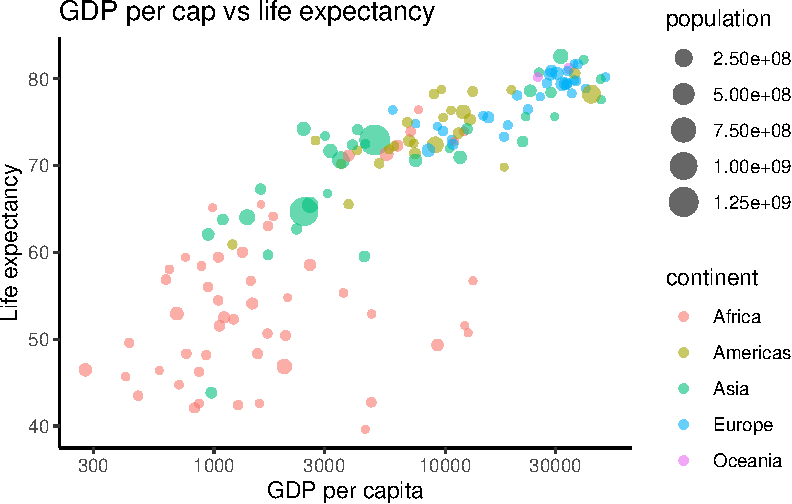
\includegraphics{06_ggplot2_files/figure-pdf/unnamed-chunk-2-1.pdf}

It's worth also noting what this chapter \emph{won't} cover, which is
the principles for creating data visualiations that tell a clear and
unambiguous story, and deciding \emph{which} data visualizations to use
to answer your specific question (or how to come up with good questions,
for that matter). I can, however, point you in the direction of some
resources that \emph{do} teach you some of these things, such as
\href{https://www.storytellingwithdata.com/books}{Storytelling with
Data} by Cole Nussbaumer Knaflic, which is a great resources for
learning how to produce effective graphics in general,
\href{https://book.rfortherestofus.com/}{R for the Rest of Us: A
Statistics-Free Introduction} by David Keyes, and even the chapter on
data visualization of my book with Bin Yu,
\href{https://vdsbook.com/05-data_viz}{Veridical Data Science}.

Fortunately, once armed with the dplyr functions from the previous
chapter, and the ggplot2 functions from this chapter, you'll have the
coding skills you need to tackle almost any dataset that comes your way.

\section{The ggplot2 canvas}\label{the-ggplot2-canvas}

To create a ggplot figure, you start by creating an empty ggplot2
``canvas'' using the \texttt{ggplot()} function. Our ``canvas'' here is
the following grey box:

\begin{Shaded}
\begin{Highlighting}[]
\FunctionTok{ggplot}\NormalTok{()}
\end{Highlighting}
\end{Shaded}


\includegraphics{06_ggplot2_files/figure-pdf/unnamed-chunk-3-1.pdf}

The first thing I need to do is to tell ggplot which dataset object
(generally, a data frame/tibble) I am going to use to create my plot,
and I do that by providing the name of my data object as the argument of
\texttt{ggplot()}:

\begin{Shaded}
\begin{Highlighting}[]
\FunctionTok{ggplot}\NormalTok{(gapminder)}
\end{Highlighting}
\end{Shaded}


\includegraphics{06_ggplot2_files/figure-pdf/unnamed-chunk-4-1.pdf}

Nothing has changed on our canvas, but now when we add some ``layers''
to our plot, ggplot can find the variables that exist within our
dataset.

To \emph{add} a layer to my plot, I literally use the plus symbol,
\texttt{+}. The name of the layer that creates a scatterplot is
\texttt{geom\_point()} (because a scattplot is made up of a collection
of ``points'').

I can add my points layer like this:

\begin{Shaded}
\begin{Highlighting}[]
\FunctionTok{ggplot}\NormalTok{(gapminder) }\SpecialCharTok{+} \FunctionTok{geom\_point}\NormalTok{()}
\end{Highlighting}
\end{Shaded}

\begin{verbatim}
Error in `geom_point()`:
! Problem while setting up geom.
i Error occurred in the 1st layer.
Caused by error in `compute_geom_1()`:
! `geom_point()` requires the following missing aesthetics: x and y.
\end{verbatim}

But I got an error because I haven't told ggplot which columns/variables
in my data I want to use to define my scatterplot. Specifically, I need
to tell it which columns should define the x- and y-coordinates of my
scatterplot points. I do that by providing an ``aesthetics'' function as
the argument of my points layer, in which I specify which column defines
the x-coordinate (\texttt{x\ =\ gdpPercap}) and which column defines the
y-coordinate (\texttt{y\ =\ lifeExp}).

\begin{Shaded}
\begin{Highlighting}[]
\FunctionTok{ggplot}\NormalTok{(gapminder) }\SpecialCharTok{+} 
  \FunctionTok{geom\_point}\NormalTok{(}\FunctionTok{aes}\NormalTok{(}\AttributeTok{x =}\NormalTok{ gdpPercap, }\AttributeTok{y =}\NormalTok{ lifeExp))}
\end{Highlighting}
\end{Shaded}

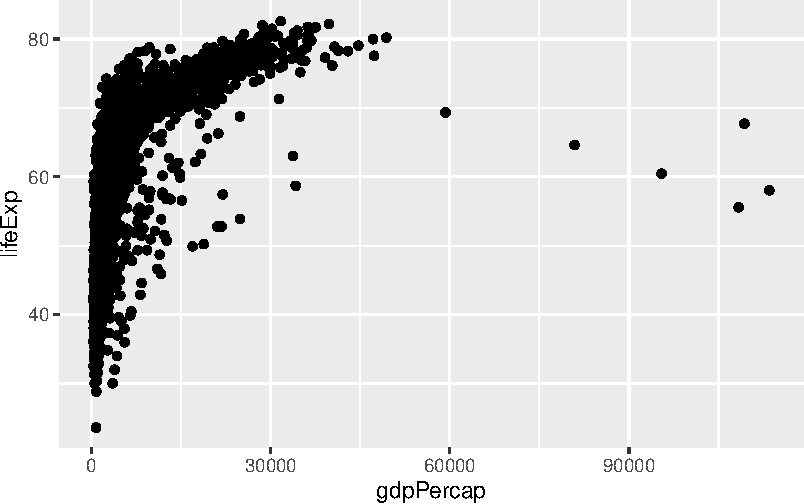
\includegraphics{06_ggplot2_files/figure-pdf/unnamed-chunk-6-1.pdf}

Now we have our scatterplot, and ggplot has even very kindly provided x-
and y-axis names! Gee, thanks!

Unfortunately ggplot is a little bit dumb, and it can only find your
data frame columns when they are referenced inside the \texttt{aes()}
function.

If I reproduced this code without the \texttt{aes()} function, I get an
error telling me that
\texttt{\textquotesingle{}gdpPercap\textquotesingle{}} cannot be found:

\begin{Shaded}
\begin{Highlighting}[]
\FunctionTok{ggplot}\NormalTok{(gapminder) }\SpecialCharTok{+} 
  \FunctionTok{geom\_point}\NormalTok{(}\AttributeTok{x =}\NormalTok{ gdpPercap, }\AttributeTok{y =}\NormalTok{ lifeExp)}
\end{Highlighting}
\end{Shaded}

\begin{verbatim}
Error in eval(expr, envir, enclos): object 'gdpPercap' not found
\end{verbatim}

Basically, if I try to reference a column from my data frame outside of
the \texttt{aes()} function, ggplot will look for an object in my space
with the same name as the column, in this case \texttt{gdpPercap}, and
it won't be able to find one!

I like to think of the aesthetics function \texttt{aes()} as a secret
code that tells ggplot that the objects I'm referring to are columns of
my data frame.

Since \texttt{ggplot()} is just a function, I can also pipe my data into
it like this:

\begin{Shaded}
\begin{Highlighting}[]
\NormalTok{gapminder }\SpecialCharTok{|\textgreater{}} 
  \FunctionTok{ggplot}\NormalTok{() }\SpecialCharTok{+} 
  \FunctionTok{geom\_point}\NormalTok{(}\FunctionTok{aes}\NormalTok{(}\AttributeTok{x =}\NormalTok{ gdpPercap, }\AttributeTok{y =}\NormalTok{ lifeExp))}
\end{Highlighting}
\end{Shaded}

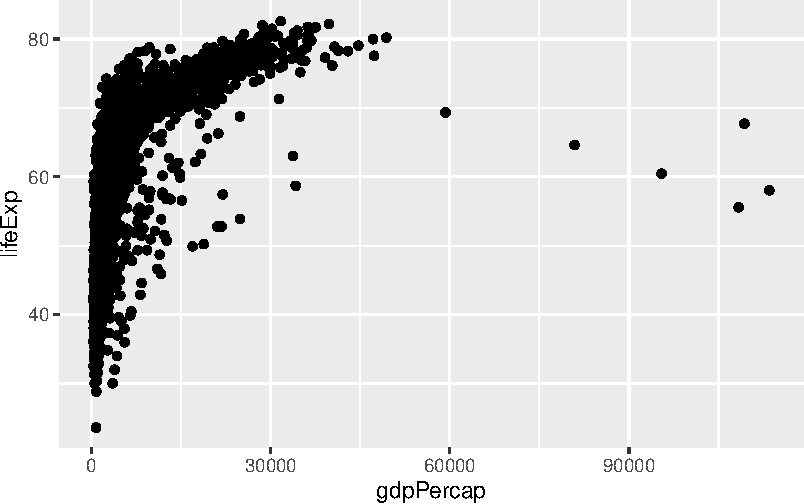
\includegraphics{06_ggplot2_files/figure-pdf/unnamed-chunk-8-1.pdf}

Why might I want to do that? I do this a lot, usually because I often
want to make minor modifications to my data before plotting it (but I
don't want to create a new intermediate object).

For example, if I want to recreate this scatterplot just for the year
2007, I could conduct a filter step and then pipe my filtered data frame
into \texttt{ggplot()}:

\begin{Shaded}
\begin{Highlighting}[]
\NormalTok{gapminder }\SpecialCharTok{|\textgreater{}}
  \FunctionTok{filter}\NormalTok{(year }\SpecialCharTok{==} \DecValTok{2007}\NormalTok{) }\SpecialCharTok{|\textgreater{}}
  \FunctionTok{ggplot}\NormalTok{() }\SpecialCharTok{+}
  \FunctionTok{geom\_point}\NormalTok{(}\FunctionTok{aes}\NormalTok{(}\AttributeTok{x =}\NormalTok{ gdpPercap, }\AttributeTok{y =}\NormalTok{ lifeExp))}
\end{Highlighting}
\end{Shaded}

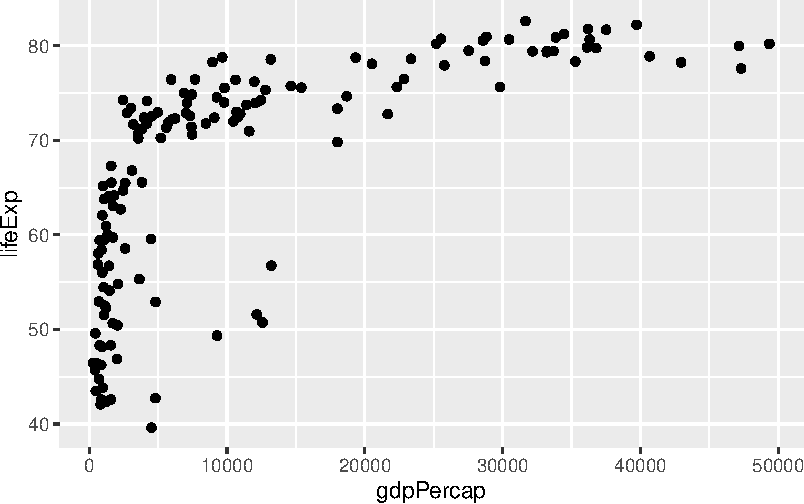
\includegraphics{06_ggplot2_files/figure-pdf/unnamed-chunk-9-1.pdf}

\section{\texorpdfstring{\texttt{+} versus
\texttt{\textbar{}\textgreater{}}}{+ versus \textbar\textgreater{}}}\label{versus}

Probably one of the most common errors I make when doing data analysis
is getting confused about when I should use \texttt{+} and when I should
use \texttt{\textbar{}\textgreater{}}.

When we are adding ggplot layers, we always use \texttt{+}, but when we
are chaining functions together, we use the pipe,
\texttt{\textbar{}\textgreater{}}.

To understand why, remember that the pipe,
\texttt{\textbar{}\textgreater{}} takes the object on the left and
places it into the first argument of the function on the right. This is
not what our ggplot2 functions are doing though, these are layering
objects on top of one another, and so they use \texttt{+} instead of
\texttt{\textbar{}\textgreater{}}.

Take a look at this code, and notice when we use \texttt{+} versus
\texttt{\textbar{}\textgreater{}}.

\begin{Shaded}
\begin{Highlighting}[]
\NormalTok{gapminder }\SpecialCharTok{|\textgreater{}}
  \FunctionTok{filter}\NormalTok{(year }\SpecialCharTok{==} \DecValTok{2007}\NormalTok{) }\SpecialCharTok{|\textgreater{}}
  \FunctionTok{ggplot}\NormalTok{() }\SpecialCharTok{+}
  \FunctionTok{geom\_point}\NormalTok{(}\FunctionTok{aes}\NormalTok{(}\AttributeTok{x =}\NormalTok{ gdpPercap, }\AttributeTok{y =}\NormalTok{ lifeExp))}
\end{Highlighting}
\end{Shaded}

The alternative to applying my filtering step and creating my plot all
at once is defining a new object just containing the gapminder data for
2007, and providing this filtered data frame object as the argument of
the \texttt{ggplot()} function:

\begin{Shaded}
\begin{Highlighting}[]
\CommentTok{\# define a new data frame}
\NormalTok{gapminder\_2007 }\OtherTok{\textless{}{-}}\NormalTok{ gapminder }\SpecialCharTok{|\textgreater{}} \FunctionTok{filter}\NormalTok{(year }\SpecialCharTok{==} \DecValTok{2007}\NormalTok{)}
\CommentTok{\# provide this data frame as the argument of my ggplot() function}
\FunctionTok{ggplot}\NormalTok{(gapminder\_2007) }\SpecialCharTok{+}
  \FunctionTok{geom\_point}\NormalTok{(}\FunctionTok{aes}\NormalTok{(}\AttributeTok{x =}\NormalTok{ gdpPercap, }\AttributeTok{y =}\NormalTok{ lifeExp))}
\end{Highlighting}
\end{Shaded}

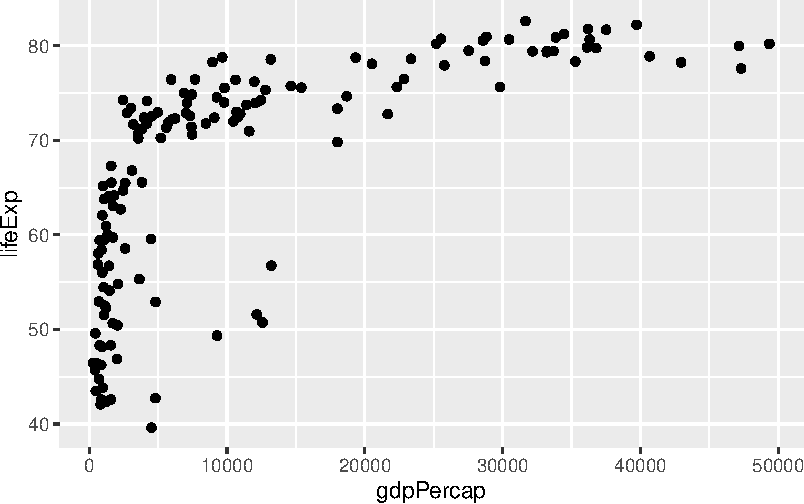
\includegraphics{06_ggplot2_files/figure-pdf/unnamed-chunk-11-1.pdf}

When do you think I might prefer to do the ``all-at-once'' approach:

\begin{Shaded}
\begin{Highlighting}[]
\NormalTok{gapminder }\SpecialCharTok{|\textgreater{}} 
  \FunctionTok{filter}\NormalTok{(year }\SpecialCharTok{==} \DecValTok{2007}\NormalTok{) }\SpecialCharTok{|\textgreater{}} 
  \FunctionTok{ggplot}\NormalTok{() }\SpecialCharTok{+}
  \FunctionTok{geom\_point}\NormalTok{(}\FunctionTok{aes}\NormalTok{(}\AttributeTok{x =}\NormalTok{ gdpPercap, }\AttributeTok{y =}\NormalTok{ lifeExp))}
\end{Highlighting}
\end{Shaded}

versus defining an intermediate \texttt{gapminder\_2007} object and then
creating my plot with \texttt{ggplot(gapminder\_2007)}:

\begin{Shaded}
\begin{Highlighting}[]
\NormalTok{gapminder\_2007 }\OtherTok{\textless{}{-}}\NormalTok{ gapminder }\SpecialCharTok{|\textgreater{}} \FunctionTok{filter}\NormalTok{(year }\SpecialCharTok{==} \DecValTok{2007}\NormalTok{)}
\FunctionTok{ggplot}\NormalTok{(gapminder\_2007) }\SpecialCharTok{+}
  \FunctionTok{geom\_point}\NormalTok{(}\FunctionTok{aes}\NormalTok{(}\AttributeTok{x =}\NormalTok{ gdpPercap, }\AttributeTok{y =}\NormalTok{ lifeExp))}
\end{Highlighting}
\end{Shaded}

Basically, if I am going to use the filtered version of data for
anything other than just this single plot (e.g., if I am going to create
several plots using just the data from 2007), then I would prefer to
define the \texttt{gapminder\_2007} object and use this in my
\texttt{ggplot()} argument, rather than conduct the filtering every
time. But if this is the only time I am going to use this 2007 data,
then I would prefer to avoid defining an unnecessary object.

In general, if you are performing the same action multiple times, for
example, to create several different plots, then it's more efficient to
create an object that you can reuse.

For instance, having defined \texttt{gapminder\_2007}, I can use it to
also create a different plot, this time a histogram of \texttt{lifeExp}
values in 2007:

\begin{Shaded}
\begin{Highlighting}[]
\FunctionTok{ggplot}\NormalTok{(gapminder\_2007) }\SpecialCharTok{+}
  \FunctionTok{geom\_histogram}\NormalTok{(}\FunctionTok{aes}\NormalTok{(}\AttributeTok{x =}\NormalTok{ lifeExp))}
\end{Highlighting}
\end{Shaded}

\begin{verbatim}
`stat_bin()` using `bins = 30`. Pick better value with `binwidth`.
\end{verbatim}

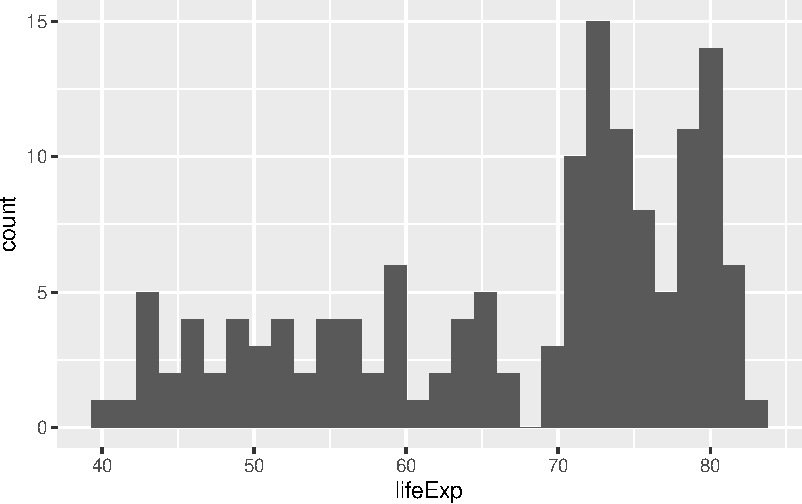
\includegraphics{06_ggplot2_files/figure-pdf/unnamed-chunk-14-1.pdf}

Note that to create a histogram using \texttt{geom\_histogram()}, I just
need to give it the x-axis variable, \texttt{lifeExp}, and it will do
all of the binning and tallying up of counts needed to determine the
y-axis for me.

\section{Exercise}

Create a ggplot scatterplot of population against life expectancy for
all countries in Europe in 2002

\section{Solution}

\begin{Shaded}
\begin{Highlighting}[]
\NormalTok{gapminder }\SpecialCharTok{|\textgreater{}}
  \FunctionTok{filter}\NormalTok{(continent }\SpecialCharTok{==} \StringTok{"Europe"}\NormalTok{, year }\SpecialCharTok{==} \DecValTok{2002}\NormalTok{) }\SpecialCharTok{|\textgreater{}}
  \FunctionTok{ggplot}\NormalTok{() }\SpecialCharTok{+} 
  \FunctionTok{geom\_point}\NormalTok{(}\FunctionTok{aes}\NormalTok{(}\AttributeTok{x =}\NormalTok{ pop, }\AttributeTok{y =}\NormalTok{ lifeExp))}
\end{Highlighting}
\end{Shaded}

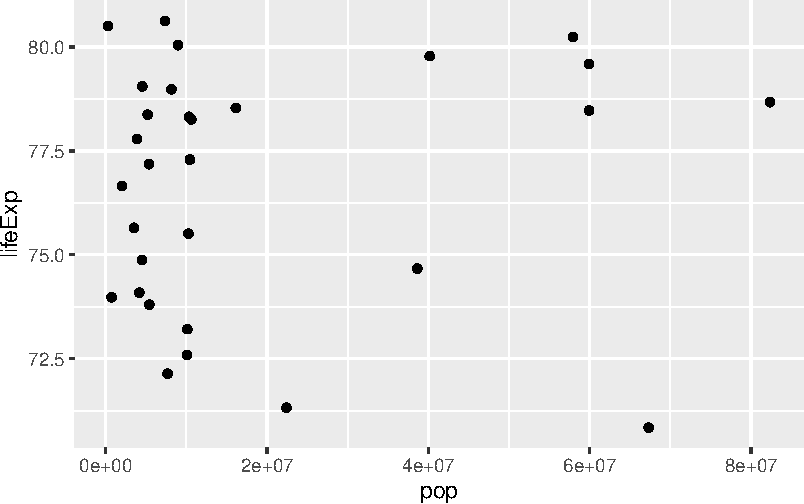
\includegraphics{06_ggplot2_files/figure-pdf/unnamed-chunk-15-1.pdf}

\section{Exercise}

Create a ggplot histogram of the GDP per capita in 2002

\section{Solution}

\begin{Shaded}
\begin{Highlighting}[]
\NormalTok{gapminder }\SpecialCharTok{|\textgreater{}}
  \FunctionTok{filter}\NormalTok{(year }\SpecialCharTok{==} \DecValTok{2002}\NormalTok{) }\SpecialCharTok{|\textgreater{}}
  \FunctionTok{ggplot}\NormalTok{() }\SpecialCharTok{+} 
  \FunctionTok{geom\_histogram}\NormalTok{(}\FunctionTok{aes}\NormalTok{(}\AttributeTok{x =}\NormalTok{ gdpPercap))}
\end{Highlighting}
\end{Shaded}

\begin{verbatim}
`stat_bin()` using `bins = 30`. Pick better value with `binwidth`.
\end{verbatim}

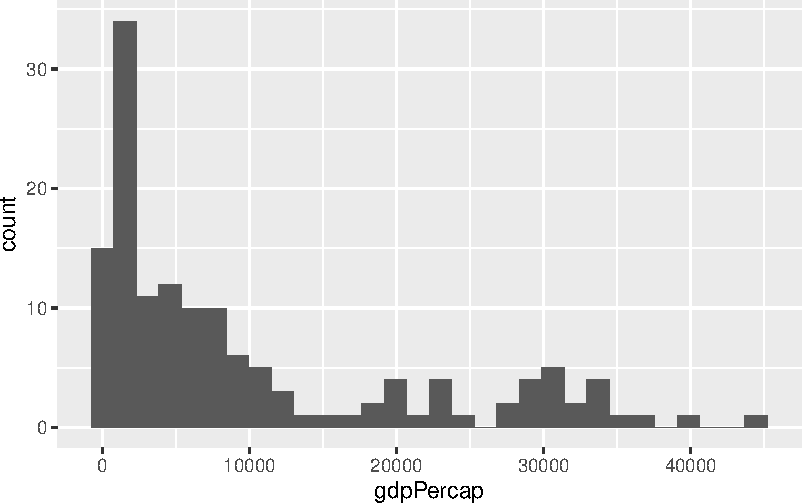
\includegraphics{06_ggplot2_files/figure-pdf/unnamed-chunk-16-1.pdf}

\section{Defining ggplot2 aesthetics}\label{defining-ggplot2-aesthetics}

\texttt{x} and \texttt{y} are ``aesthetic'' properties of the points in
a scatterplot, and \texttt{x} is an ``aesthetic'' property of the bars
in a histogram. But they aren't the \emph{only} aesthetic properties
that we can specify!

For example, some other scatterplot aesthetic properties that we can
specify include \texttt{color}, \texttt{size}, and \texttt{shape}.

You can specify the \texttt{color} of the points using the
\texttt{color} aesthetic:

\begin{Shaded}
\begin{Highlighting}[]
\FunctionTok{ggplot}\NormalTok{(gapminder\_2007) }\SpecialCharTok{+} 
  \FunctionTok{geom\_point}\NormalTok{(}\FunctionTok{aes}\NormalTok{(}\AttributeTok{x =}\NormalTok{ gdpPercap, }\AttributeTok{y =}\NormalTok{ lifeExp, }\AttributeTok{color =}\NormalTok{ continent))}
\end{Highlighting}
\end{Shaded}

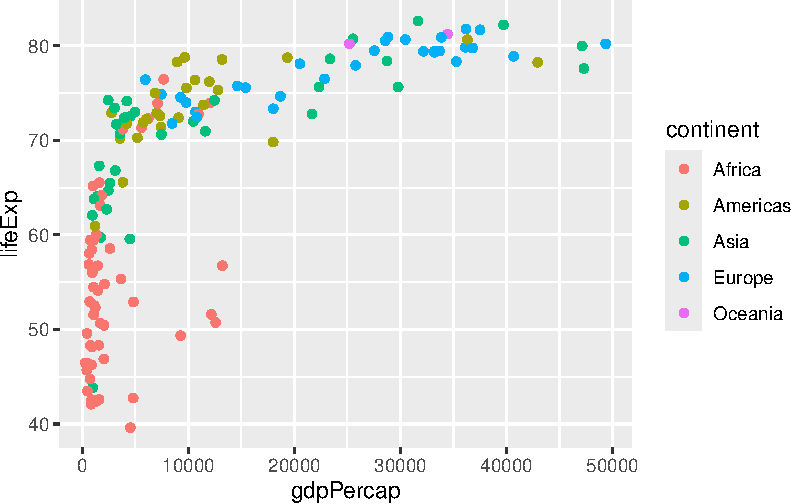
\includegraphics{06_ggplot2_files/figure-pdf/unnamed-chunk-17-1.pdf}

In this example, I'm specifying \texttt{color\ =\ continent} inside the
\texttt{aes()} function, which, because it is inside the \texttt{aes()}
function, this tells ggplot2 that \texttt{continent} is a column in my
data and that it should come up with a unique color for each unique
\texttt{continent} value.

What if I wanted to just make all of the points in my scatterplot
``blue'' instead of based on the continent column, like this:

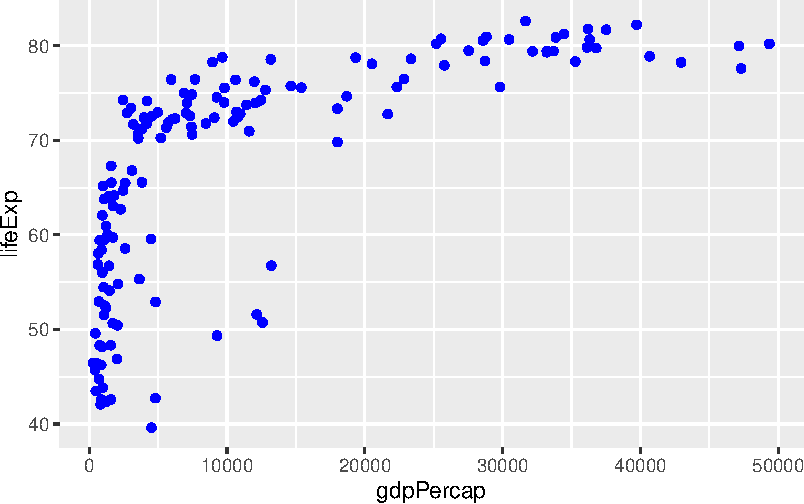
\includegraphics{06_ggplot2_files/figure-pdf/unnamed-chunk-18-1.pdf}

If I try to just replace \texttt{color\ =\ continent} with
\texttt{color\ =\ "blue"} (where I'm providing quotes around ``blue''
because I want to specifically pass the \emph{character} value ``blue'',
not a column or variable callued \texttt{blue}), it doesn't work:

\begin{Shaded}
\begin{Highlighting}[]
\FunctionTok{ggplot}\NormalTok{(gapminder\_2007) }\SpecialCharTok{+} 
  \FunctionTok{geom\_point}\NormalTok{(}\FunctionTok{aes}\NormalTok{(}\AttributeTok{x =}\NormalTok{ gdpPercap, }\AttributeTok{y =}\NormalTok{ lifeExp, }\AttributeTok{color =} \StringTok{"blue"}\NormalTok{))}
\end{Highlighting}
\end{Shaded}

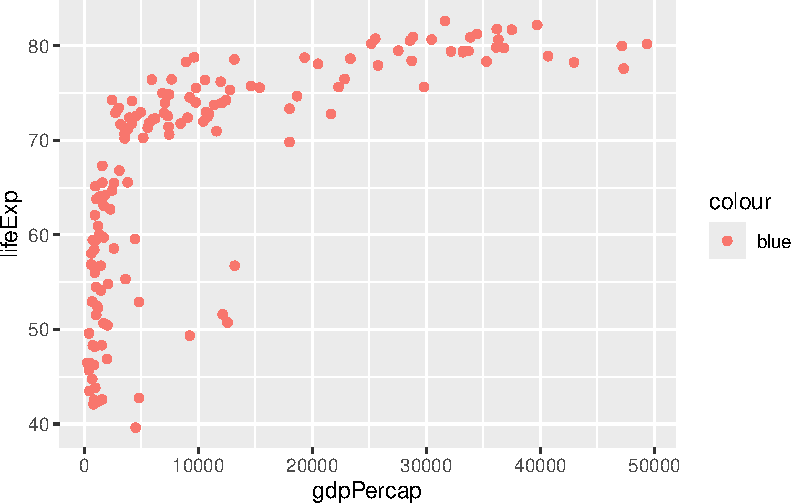
\includegraphics{06_ggplot2_files/figure-pdf/unnamed-chunk-19-1.pdf}

Since \texttt{color\ =\ "blue"} is specified \emph{inside} the
\texttt{aes()} function, ggplot is looking for a column inside the
\texttt{gapminder} data frame called \texttt{"blue"}, and since it can't
find one, it just creates one and populates it entirely with the value
``blue'' for all data points, so what we end up with is a scatterplot
whose color is deteremined by a categorical variable whose value
consists of a single value, which is just the word ``blue'', and since
this variable only has a single value, ggplot only provides one color,
and this color is just the first default ggplot2 color which is this
nice ``salmony'' color.

If you want to define an aesthetic of your plot that does \emph{not}
depend on a column in your data, you need to specify it \emph{outside}
the \texttt{aes()} function. If we just move the
\texttt{color\ =\ "blue"} argument \emph{outside} \texttt{aes()}, we get
what we wanted:

\begin{Shaded}
\begin{Highlighting}[]
\FunctionTok{ggplot}\NormalTok{(gapminder\_2007) }\SpecialCharTok{+} 
  \FunctionTok{geom\_point}\NormalTok{(}\FunctionTok{aes}\NormalTok{(}\AttributeTok{x =}\NormalTok{ gdpPercap, }\AttributeTok{y =}\NormalTok{ lifeExp), }\AttributeTok{color =} \StringTok{"blue"}\NormalTok{)}
\end{Highlighting}
\end{Shaded}

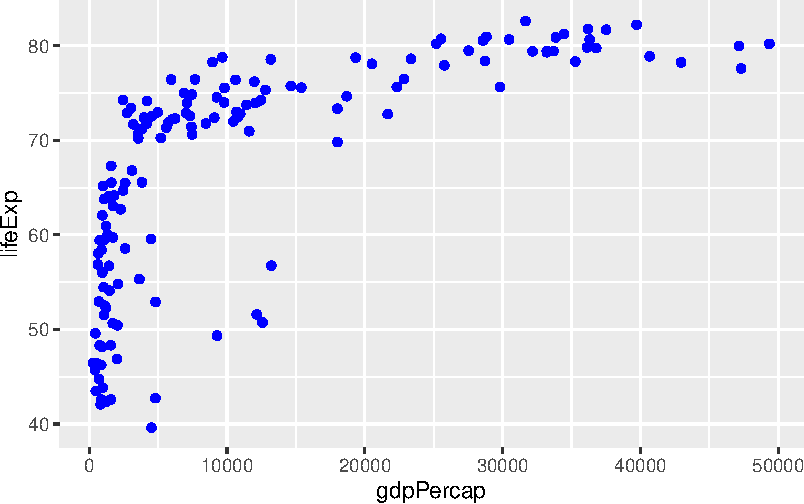
\includegraphics{06_ggplot2_files/figure-pdf/unnamed-chunk-20-1.pdf}

\section{Exercise}

Recreate the scatterplot of \texttt{lifeExp} and \texttt{gdpPercap} in
2007, but use the \texttt{continent} column to specify the
\texttt{shape} aesthetic

\section{Solution}

\begin{Shaded}
\begin{Highlighting}[]
\FunctionTok{ggplot}\NormalTok{(gapminder\_2007) }\SpecialCharTok{+} 
  \FunctionTok{geom\_point}\NormalTok{(}\FunctionTok{aes}\NormalTok{(}\AttributeTok{x =}\NormalTok{ gdpPercap, }
                 \AttributeTok{y =}\NormalTok{ lifeExp, }
                 \AttributeTok{shape =}\NormalTok{ continent))}
\end{Highlighting}
\end{Shaded}

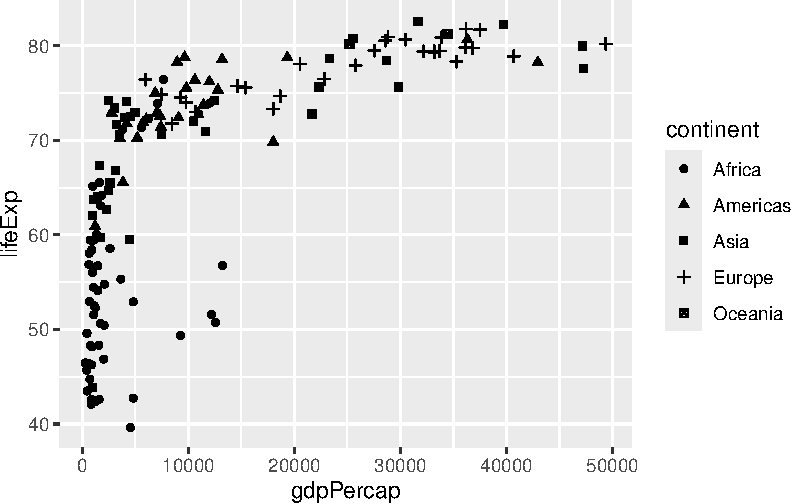
\includegraphics{06_ggplot2_files/figure-pdf/unnamed-chunk-21-1.pdf}

\section{Exercise}

Recreate the scatterplot of \texttt{lifeExp} and \texttt{gdpPercap} in
2007, but make all points have a ``triangle'' shape.

\section{Solution}

\begin{Shaded}
\begin{Highlighting}[]
\FunctionTok{ggplot}\NormalTok{(gapminder\_2007) }\SpecialCharTok{+} 
  \FunctionTok{geom\_point}\NormalTok{(}\FunctionTok{aes}\NormalTok{(}\AttributeTok{x =}\NormalTok{ gdpPercap, }
                 \AttributeTok{y =}\NormalTok{ lifeExp), }
             \AttributeTok{shape =} \StringTok{"triangle"}\NormalTok{)}
\end{Highlighting}
\end{Shaded}

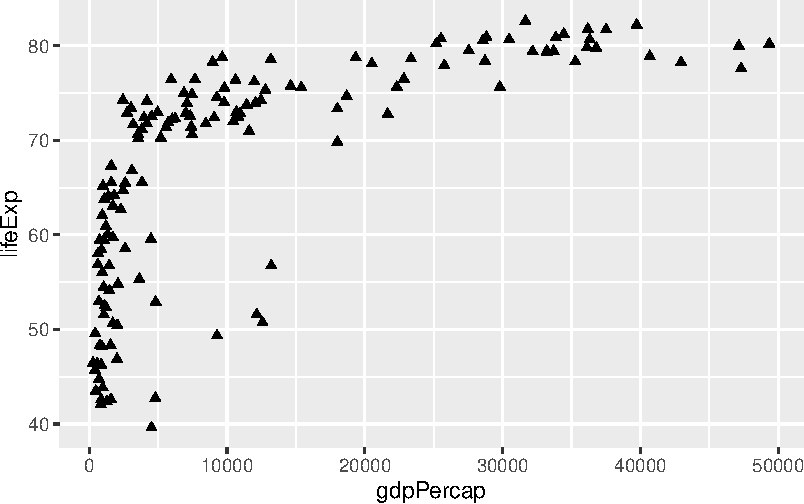
\includegraphics{06_ggplot2_files/figure-pdf/unnamed-chunk-22-1.pdf}

\subsection{Transparency}\label{transparency}

Sometimes when you have a lot of data points all sitting ontop of one
another, it can be helpful to add some transparency. You can do this
using the \texttt{alpha} argument.

\texttt{alpha} takes values between 0 and 1. \texttt{alpha\ =\ 1} is not
transparent at all, and \texttt{alpha\ =\ 0} is completely transparent.
The scatterplot below has \texttt{alpha\ =\ 0.5}:

\begin{Shaded}
\begin{Highlighting}[]
\FunctionTok{ggplot}\NormalTok{(gapminder\_2007) }\SpecialCharTok{+} 
  \FunctionTok{geom\_point}\NormalTok{(}\FunctionTok{aes}\NormalTok{(}\AttributeTok{x =}\NormalTok{ gdpPercap, }\AttributeTok{y =}\NormalTok{ lifeExp), }
             \AttributeTok{alpha =} \FloatTok{0.5}\NormalTok{)}
\end{Highlighting}
\end{Shaded}

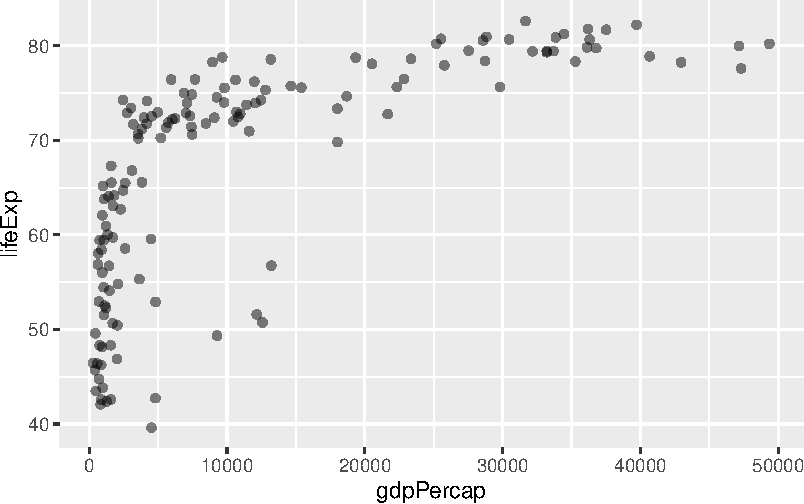
\includegraphics{06_ggplot2_files/figure-pdf/unnamed-chunk-23-1.pdf}

Since we are not using a column/variable in the data frame to specify
\texttt{alpha}, note that it is \emph{outside} the \texttt{aes()}
function of \texttt{geom\_point()}.

\section{Exercise}

Recreate the 2007 \texttt{gdpPercap} vs \texttt{lifeExp} plot where each
point has color determined by \texttt{continent}, size determined by
\texttt{pop}, and all the points have a transparency of 0.5.

\section{Solution}

\begin{Shaded}
\begin{Highlighting}[]
\FunctionTok{ggplot}\NormalTok{(gapminder\_2007) }\SpecialCharTok{+} 
  \FunctionTok{geom\_point}\NormalTok{(}\FunctionTok{aes}\NormalTok{(}\AttributeTok{x =}\NormalTok{ gdpPercap, }\AttributeTok{y =}\NormalTok{ lifeExp, }
                 \AttributeTok{color =}\NormalTok{ continent, }\AttributeTok{size =}\NormalTok{ pop), }
             \AttributeTok{alpha =} \FloatTok{0.5}\NormalTok{)}
\end{Highlighting}
\end{Shaded}

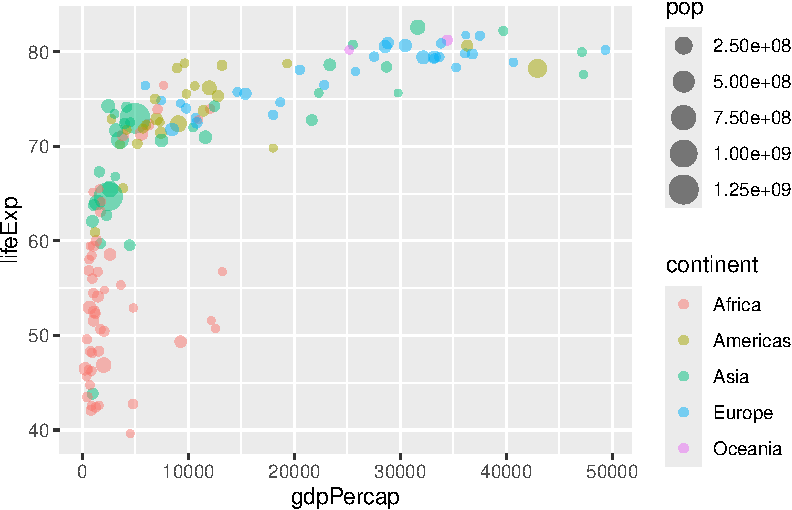
\includegraphics{06_ggplot2_files/figure-pdf/unnamed-chunk-24-1.pdf}

\section{Other kinds of plots}\label{other-kinds-of-plots}

\subsection{Line plots}\label{line-plots}

Line plots are great for showing how things change over time.

If I want to see how \texttt{lifeExp} changes by year, I can try to
create a line plot using \texttt{geom\_line()} with \texttt{lifeExp} on
the y-axis, and \texttt{year} on the x-axis:

\begin{Shaded}
\begin{Highlighting}[]
\FunctionTok{ggplot}\NormalTok{(gapminder) }\SpecialCharTok{+} 
  \FunctionTok{geom\_line}\NormalTok{(}\FunctionTok{aes}\NormalTok{(}\AttributeTok{x =}\NormalTok{ year, }
                \AttributeTok{y =}\NormalTok{ lifeExp))}
\end{Highlighting}
\end{Shaded}

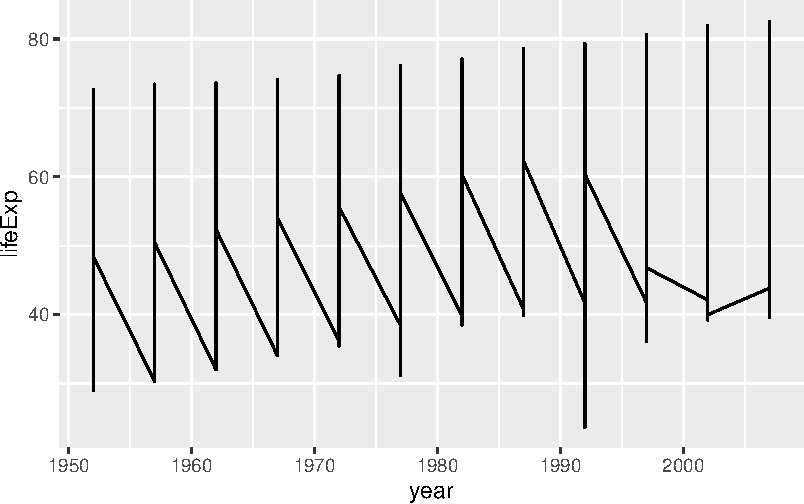
\includegraphics{06_ggplot2_files/figure-pdf/unnamed-chunk-25-1.pdf}

Ugh. gross. I don't like this plot at all. It looks terrible. What's
with all the zigzags?

Can you figure out what's going on in this plot? As a hint\ldots{} how
many \texttt{lifeExp} values do we have for each \texttt{year}? We have
many! One for each country (and there are almost 200 countries!)

Here are all the \texttt{lifeExp} values corresponding to 1962

\begin{Shaded}
\begin{Highlighting}[]
\NormalTok{gapminder }\SpecialCharTok{|\textgreater{}}
  \FunctionTok{filter}\NormalTok{(year }\SpecialCharTok{==} \DecValTok{1962}\NormalTok{) }\SpecialCharTok{|\textgreater{}} 
  \FunctionTok{select}\NormalTok{(year, country, lifeExp)}
\end{Highlighting}
\end{Shaded}

\begin{verbatim}
# A tibble: 142 x 3
    year country     lifeExp
   <dbl> <chr>         <dbl>
 1  1962 Afghanistan    32.0
 2  1962 Albania        64.8
 3  1962 Algeria        48.3
 4  1962 Angola         34  
 5  1962 Argentina      65.1
 6  1962 Australia      70.9
 7  1962 Austria        69.5
 8  1962 Bahrain        56.9
 9  1962 Bangladesh     41.2
10  1962 Belgium        70.2
# i 132 more rows
\end{verbatim}

so the vertical lines we see in our ``line plot'' above correspond to
the range of \texttt{lifeExp} values for each year, and then it probably
just connects the final \texttt{lifeExp} value that year to the first
\texttt{lifeExp} value for the next year, and those are the diagonal
lines that we see.

In general, to create a single line, we want just \emph{one} value for
the y-axis (e.g., \texttt{lifeExp}) per x-axis value (e.g.,
\texttt{year}). To satisfy this requirement, we can look at the data for
just \emph{one} country

\begin{Shaded}
\begin{Highlighting}[]
\NormalTok{gapminder }\SpecialCharTok{|\textgreater{}} 
  \FunctionTok{filter}\NormalTok{(country }\SpecialCharTok{==} \StringTok{"Australia"}\NormalTok{) }\SpecialCharTok{|\textgreater{}}
  \FunctionTok{select}\NormalTok{(year, country, lifeExp)}
\end{Highlighting}
\end{Shaded}

\begin{verbatim}
# A tibble: 12 x 3
    year country   lifeExp
   <dbl> <chr>       <dbl>
 1  1952 Australia    69.1
 2  1957 Australia    70.3
 3  1962 Australia    70.9
 4  1967 Australia    71.1
 5  1972 Australia    71.9
 6  1977 Australia    73.5
 7  1982 Australia    74.7
 8  1987 Australia    76.3
 9  1992 Australia    77.6
10  1997 Australia    78.8
11  2002 Australia    80.4
12  2007 Australia    81.2
\end{verbatim}

Now, we have just one \texttt{lifeExp} value for each \texttt{year}, and
we could create a line plot using these values:

\begin{Shaded}
\begin{Highlighting}[]
\NormalTok{gapminder }\SpecialCharTok{|\textgreater{}} 
  \FunctionTok{filter}\NormalTok{(country }\SpecialCharTok{==} \StringTok{"Australia"}\NormalTok{) }\SpecialCharTok{|\textgreater{}}
  \FunctionTok{ggplot}\NormalTok{() }\SpecialCharTok{+}
  \FunctionTok{geom\_line}\NormalTok{(}\FunctionTok{aes}\NormalTok{(}\AttributeTok{x =}\NormalTok{ year, }\AttributeTok{y =}\NormalTok{ lifeExp))}
\end{Highlighting}
\end{Shaded}

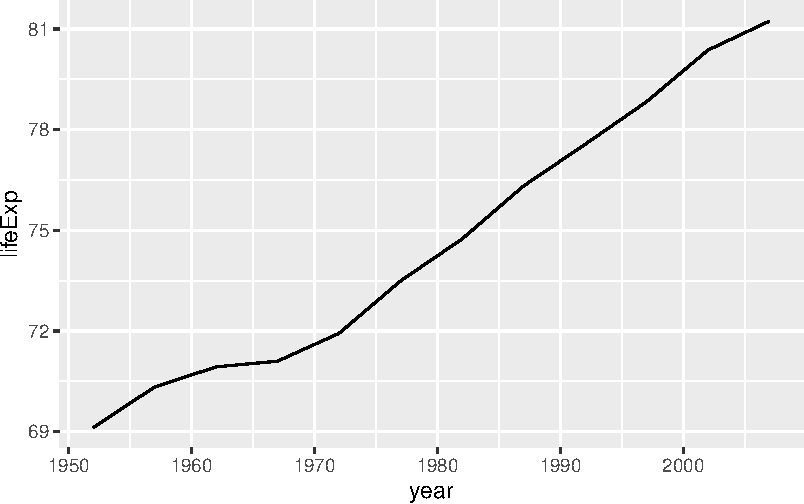
\includegraphics{06_ggplot2_files/figure-pdf/unnamed-chunk-28-1.pdf}

Gee wiz! That looks way better! It's a single line, and boy-oh-boy it
sure looks like we Aussies are living longer and longer! Onya Mate!

I could make the same plot for the US, by filtering to the US instead of
Australia:

\begin{Shaded}
\begin{Highlighting}[]
\NormalTok{gapminder }\SpecialCharTok{|\textgreater{}} 
  \FunctionTok{filter}\NormalTok{(country }\SpecialCharTok{==} \StringTok{"United States"}\NormalTok{) }\SpecialCharTok{|\textgreater{}}
  \FunctionTok{ggplot}\NormalTok{() }\SpecialCharTok{+}
  \FunctionTok{geom\_line}\NormalTok{(}\FunctionTok{aes}\NormalTok{(}\AttributeTok{x =}\NormalTok{ year, }\AttributeTok{y =}\NormalTok{ lifeExp))}
\end{Highlighting}
\end{Shaded}

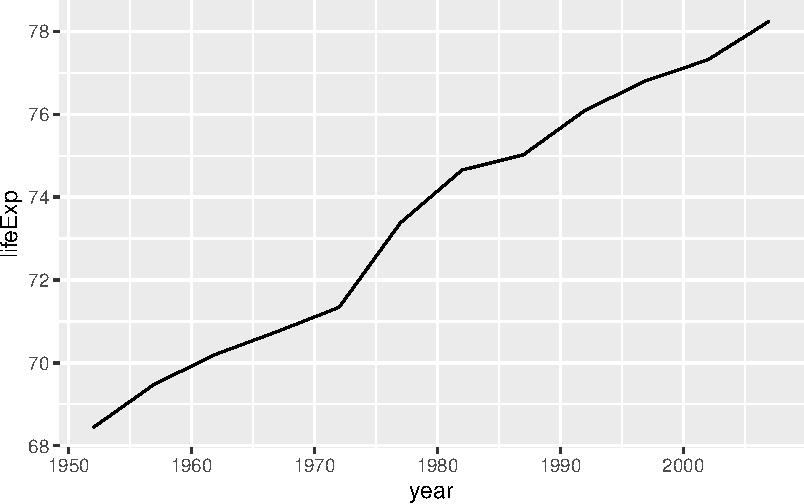
\includegraphics{06_ggplot2_files/figure-pdf/unnamed-chunk-29-1.pdf}

What if I wanted to make a plot with \emph{both} of these lines on it?

Well there are a few ways I could do that. One is good, and another is
not so good.

I'll show you the not-so-good approach first, just so you can really
appreciate the good approach.

The not-so-good approach involfe creating data frames for Australia and
the US and adding multiple line layers. The first line layer will be
just using \texttt{gapminder\_us}, the data frame for the US and the
second line layer will have its own \texttt{data} argument to which I'll
pass \texttt{gapminder\_au}, the data frame for Australia:

\begin{Shaded}
\begin{Highlighting}[]
\CommentTok{\# define the data frame for the US}
\NormalTok{gapminder\_us }\OtherTok{\textless{}{-}}\NormalTok{ gapminder }\SpecialCharTok{|\textgreater{}}
  \FunctionTok{filter}\NormalTok{(country }\SpecialCharTok{==} \StringTok{"United States"}\NormalTok{)}

\CommentTok{\# define the data frame for the australia}
\NormalTok{gapminder\_au }\OtherTok{\textless{}{-}}\NormalTok{ gapminder }\SpecialCharTok{|\textgreater{}}
  \FunctionTok{filter}\NormalTok{(country }\SpecialCharTok{==} \StringTok{"Australia"}\NormalTok{)}

\CommentTok{\# Create a line plot for the US and then add a line plot layer for Australia}
\FunctionTok{ggplot}\NormalTok{(gapminder\_us) }\SpecialCharTok{+}
  \FunctionTok{geom\_line}\NormalTok{(}\FunctionTok{aes}\NormalTok{(}\AttributeTok{x =}\NormalTok{ year, }\AttributeTok{y =}\NormalTok{ lifeExp)) }\SpecialCharTok{+}
  \FunctionTok{geom\_line}\NormalTok{(}\FunctionTok{aes}\NormalTok{(}\AttributeTok{x =}\NormalTok{ year, }\AttributeTok{y =}\NormalTok{ lifeExp),}
            \AttributeTok{data =}\NormalTok{ gapminder\_au)}
\end{Highlighting}
\end{Shaded}

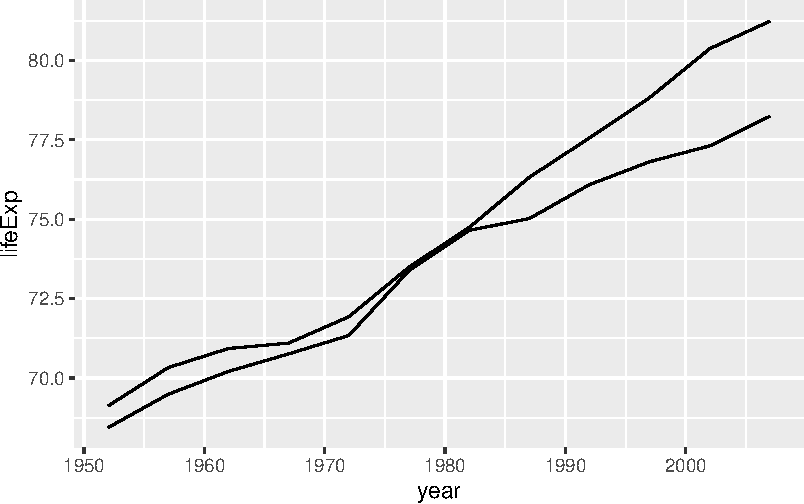
\includegraphics{06_ggplot2_files/figure-pdf/unnamed-chunk-30-1.pdf}

Here the first \texttt{geom\_line()} layer is based on the
\texttt{gapminder\_us} data frame provided as the argument of
\texttt{ggplot()}, and the second one is based on the
\texttt{gapminder\_au} data frame provided in the \texttt{data} argument
of the second \texttt{geom\_line()} layer (when you don't provide a
\texttt{data} argument, each layer will be based on the data frame
provided to \texttt{ggplot()})

While this technically works, this approach sucks for a few reasons.
First, I can't tell which line is which. There is no legend (and it's
unfortunately not all that easy to add a legend manually to a ggplot2
figure). Another reason this approach sucks is that it's not scalable.
If I wanted to do this for 10 countries, I'd have to create 10 different
data frames and add 10 line layers to my plot! No thanks.

Instead of adding separate line layers for each country, I can instead
use the \texttt{color} or \texttt{group} aesthetic to tell
\texttt{ggplot()} that I want separate lines for each country, say.

In the code below, I create a data frame that contains the data for both
Australia and the US, and then I create a ggplot2 line plot, specifying
\texttt{color\ =\ country} inside my \texttt{aes()} function, which will
give me a separate line for each country:

\begin{Shaded}
\begin{Highlighting}[]
\NormalTok{gapminder }\SpecialCharTok{|\textgreater{}}
  \FunctionTok{filter}\NormalTok{(country }\SpecialCharTok{\%in\%} \FunctionTok{c}\NormalTok{(}\StringTok{"Australia"}\NormalTok{, }\StringTok{"United States"}\NormalTok{)) }\SpecialCharTok{|\textgreater{}}
  \FunctionTok{ggplot}\NormalTok{() }\SpecialCharTok{+}
  \FunctionTok{geom\_line}\NormalTok{(}\FunctionTok{aes}\NormalTok{(}\AttributeTok{x =}\NormalTok{ year, }\AttributeTok{y =}\NormalTok{ lifeExp, }\AttributeTok{color =}\NormalTok{ country))}
\end{Highlighting}
\end{Shaded}

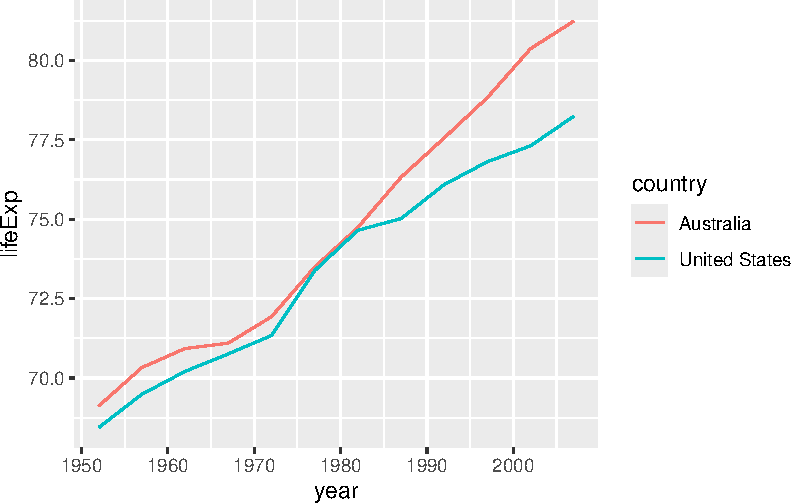
\includegraphics{06_ggplot2_files/figure-pdf/unnamed-chunk-31-1.pdf}

An alternative if I want a separate line for each country, but I don't
want each line to have a different color, is to use the \texttt{group}
aesthetic instead of the \texttt{color} aesthetic:

\begin{Shaded}
\begin{Highlighting}[]
\NormalTok{gapminder }\SpecialCharTok{|\textgreater{}}
  \FunctionTok{filter}\NormalTok{(country }\SpecialCharTok{\%in\%} \FunctionTok{c}\NormalTok{(}\StringTok{"Australia"}\NormalTok{, }\StringTok{"United States"}\NormalTok{)) }\SpecialCharTok{|\textgreater{}}
  \FunctionTok{ggplot}\NormalTok{() }\SpecialCharTok{+}
  \FunctionTok{geom\_line}\NormalTok{(}\FunctionTok{aes}\NormalTok{(}\AttributeTok{x =}\NormalTok{ year, }\AttributeTok{y =}\NormalTok{ lifeExp, }\AttributeTok{group =}\NormalTok{ country))}
\end{Highlighting}
\end{Shaded}

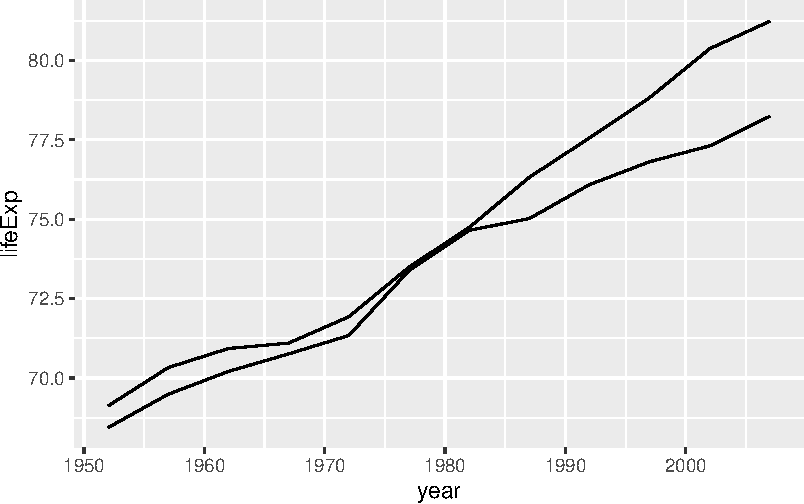
\includegraphics{06_ggplot2_files/figure-pdf/unnamed-chunk-32-1.pdf}

The following code create a line plot of lifeExp by year for each
country on the Americas content (with no colors or legend).

\begin{Shaded}
\begin{Highlighting}[]
\NormalTok{gapminder }\SpecialCharTok{|\textgreater{}} 
  \FunctionTok{filter}\NormalTok{(continent }\SpecialCharTok{==} \StringTok{"Americas"}\NormalTok{) }\SpecialCharTok{|\textgreater{}} 
  \FunctionTok{ggplot}\NormalTok{() }\SpecialCharTok{+} 
  \FunctionTok{geom\_line}\NormalTok{(}\FunctionTok{aes}\NormalTok{(}\AttributeTok{x =}\NormalTok{ year, }
                \AttributeTok{y =}\NormalTok{ lifeExp, }
                \AttributeTok{group =}\NormalTok{ country))}
\end{Highlighting}
\end{Shaded}

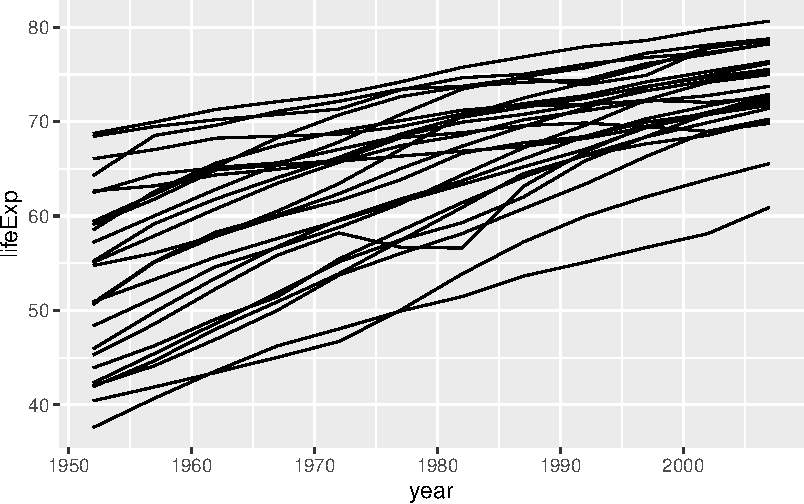
\includegraphics{06_ggplot2_files/figure-pdf/unnamed-chunk-33-1.pdf}

\section{Exercise}

Compute the average life expectancy for each continent for each year,
and then create a line plot of the average life expectancy for each
continent over time (each continent should have it's own different
colored line).

Here is an example of the plot I want you to make:

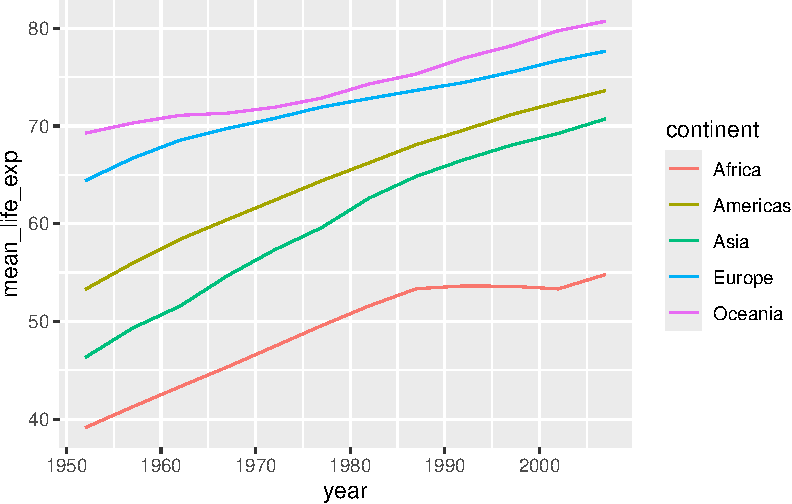
\includegraphics{06_ggplot2_files/figure-pdf/unnamed-chunk-34-1.pdf}

\section{Solution}

\begin{Shaded}
\begin{Highlighting}[]
\NormalTok{gapminder }\SpecialCharTok{|\textgreater{}} 
  \FunctionTok{group\_by}\NormalTok{(continent, year) }\SpecialCharTok{|\textgreater{}} 
  \FunctionTok{summarize}\NormalTok{(}\AttributeTok{mean\_life\_exp =} \FunctionTok{mean}\NormalTok{(lifeExp)) }\SpecialCharTok{|\textgreater{}} 
  \FunctionTok{ggplot}\NormalTok{() }\SpecialCharTok{+}
  \FunctionTok{geom\_line}\NormalTok{(}\FunctionTok{aes}\NormalTok{(}\AttributeTok{x =}\NormalTok{ year, }
                \AttributeTok{y =}\NormalTok{ mean\_life\_exp, }
                \AttributeTok{color =}\NormalTok{ continent))}
\end{Highlighting}
\end{Shaded}

\begin{verbatim}
`summarise()` has grouped output by 'continent'. You can override using the
`.groups` argument.
\end{verbatim}

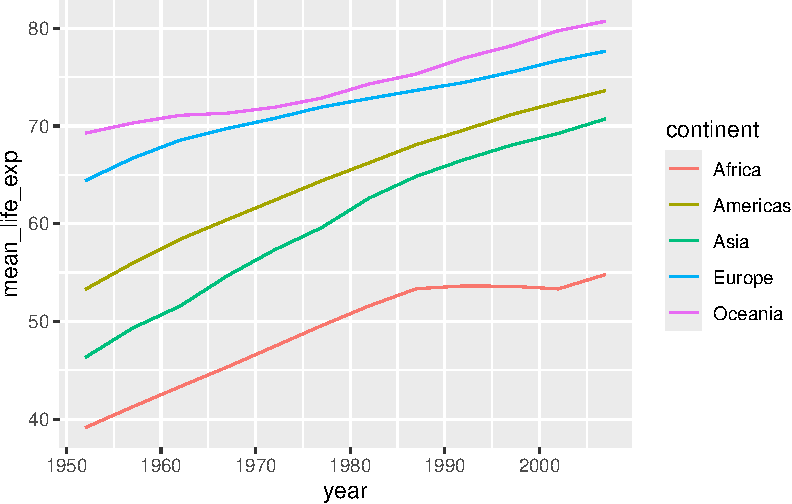
\includegraphics{06_ggplot2_files/figure-pdf/unnamed-chunk-35-1.pdf}

\subsection{Boxplots}\label{boxplots}

Like scatterplots created with \texttt{geom\_point()}, boxplots created
with a \texttt{geom\_boxplot()} layer desire an \texttt{x} and a
\texttt{y} aesthetic, however, unlike \texttt{geom\_point()} which wants
both the \texttt{x} and \texttt{y} variables to be continuous numeric
variables, \texttt{geom\_boxplot()} wants \emph{one} of the \texttt{x}
and \texttt{y} aesthetics to be a categorical (character or factor)
variable and the other one to be numeric--\texttt{geom\_boxplot()} will
create a separate boxplot for each categorical value.

For example, below we create a boxplot of \texttt{lifeExp} for each
value of \texttt{continent}:

\begin{Shaded}
\begin{Highlighting}[]
\FunctionTok{ggplot}\NormalTok{(gapminder) }\SpecialCharTok{+} 
  \FunctionTok{geom\_boxplot}\NormalTok{(}\FunctionTok{aes}\NormalTok{(}\AttributeTok{x =}\NormalTok{ continent, }\AttributeTok{y =}\NormalTok{ lifeExp))}
\end{Highlighting}
\end{Shaded}

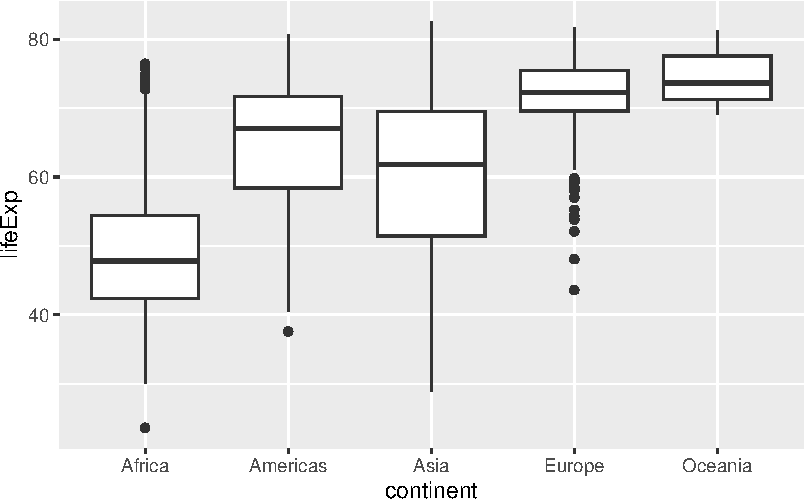
\includegraphics{06_ggplot2_files/figure-pdf/unnamed-chunk-36-1.pdf}

The bottom of the box of a boxplot corresponds to \(Q_1\), the first
quartile of the variable (the value for which 25\% of values are less
than it) and the top of the box corresponds to the third quartile,
\(Q_3\) of the variable (the value for which 75\% of values are less
than it). The bar in the middle is the median, which corresponds to the
second quartile, \(Q_2\) (the value for which 50\% of values are less
than it). The lines that extend from the bottom and top of the boxplot
reach as far as \(Q_1 - 1.5 (Q_3 - Q_1)\) and \(Q_3 + 1.5 (Q_3 - Q_1)\),
respectively, and all values that are outside this range are shown as
points and are called ``outliers.''

If you switch the \texttt{x} and the \texttt{y} so that the \texttt{y}
aesthetic is the categorical/character \texttt{continent} variable, then
you get horizontal boxplots instead.

\begin{Shaded}
\begin{Highlighting}[]
\FunctionTok{ggplot}\NormalTok{(gapminder) }\SpecialCharTok{+} 
  \FunctionTok{geom\_boxplot}\NormalTok{(}\FunctionTok{aes}\NormalTok{(}\AttributeTok{x =}\NormalTok{ lifeExp, }\AttributeTok{y =}\NormalTok{ continent))}
\end{Highlighting}
\end{Shaded}

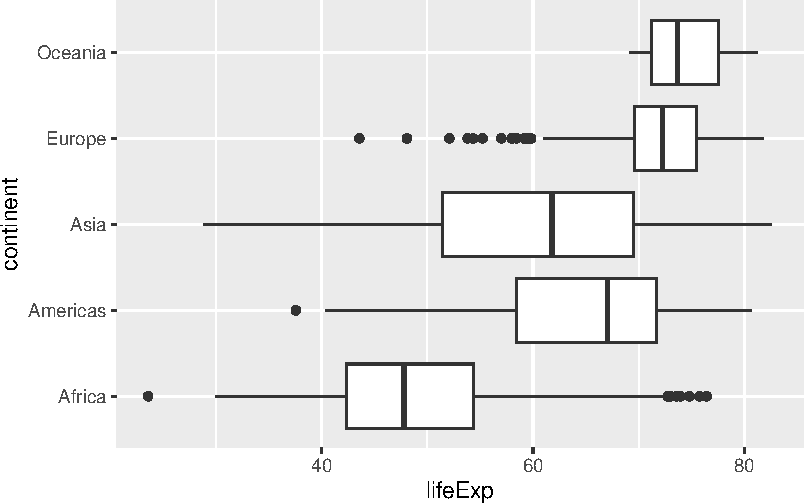
\includegraphics{06_ggplot2_files/figure-pdf/unnamed-chunk-37-1.pdf}

\texttt{geom\_boxplot()} is great for creating side-by-side boxplots for
the different levels/values of a categorical variable.

But you can create single boxplots for an entire variable, such as
\texttt{lifeExp}, by just providing \texttt{y\ =\ lifeExp} to your
aesthetic function (leaving \texttt{x} out entirely):

\begin{Shaded}
\begin{Highlighting}[]
\FunctionTok{ggplot}\NormalTok{(gapminder) }\SpecialCharTok{+} 
  \FunctionTok{geom\_boxplot}\NormalTok{(}\FunctionTok{aes}\NormalTok{(}\AttributeTok{y =}\NormalTok{ lifeExp))}
\end{Highlighting}
\end{Shaded}

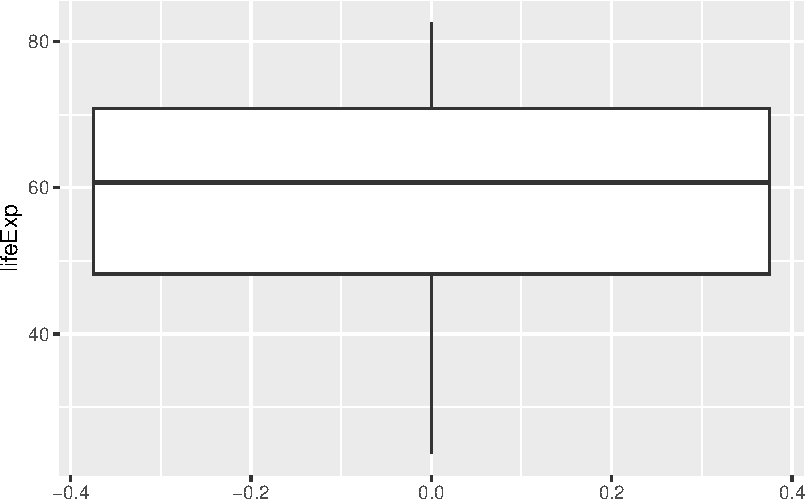
\includegraphics{06_ggplot2_files/figure-pdf/unnamed-chunk-38-1.pdf}

But I rarely do this--I find that boxplots are most helpful for
\emph{comparing} the distributions of a variable across different
groups.

\subsection{Histograms}\label{histograms}

If I want to look at the distribution of a single variable, I find it
more useful to use a histogram, such as the histogram of
\texttt{lifeExp} below:

\begin{Shaded}
\begin{Highlighting}[]
\FunctionTok{ggplot}\NormalTok{(gapminder) }\SpecialCharTok{+} 
  \FunctionTok{geom\_histogram}\NormalTok{(}\FunctionTok{aes}\NormalTok{(}\AttributeTok{x =}\NormalTok{ lifeExp))}
\end{Highlighting}
\end{Shaded}

\begin{verbatim}
`stat_bin()` using `bins = 30`. Pick better value with `binwidth`.
\end{verbatim}

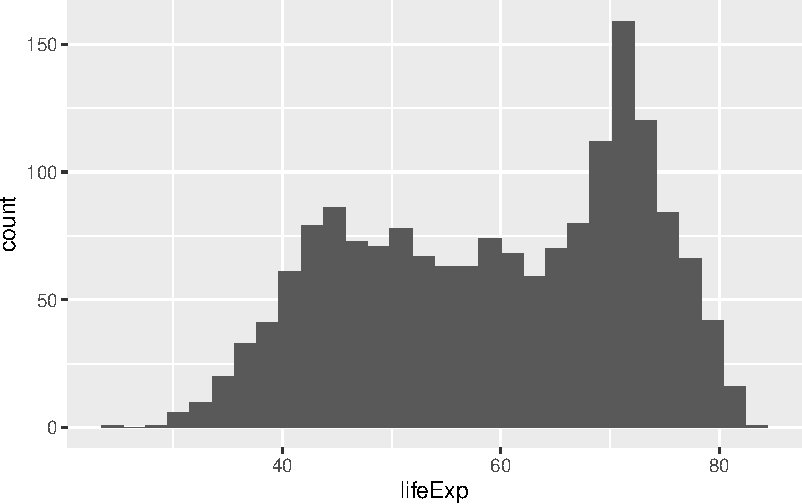
\includegraphics{06_ggplot2_files/figure-pdf/unnamed-chunk-39-1.pdf}

A histogram essentially takes the range of a continuous numeric
variable, chops it up into binned intervals, and then uses bars to
represent how many values fall into each binned interval.

I don't really like that the histogram doesn't provide outlines for each
of the bars, so I often add them in by providing a \texttt{color} value
\emph{outside} the \texttt{aes()} function:

\begin{Shaded}
\begin{Highlighting}[]
\FunctionTok{ggplot}\NormalTok{(gapminder) }\SpecialCharTok{+} 
  \FunctionTok{geom\_histogram}\NormalTok{(}\FunctionTok{aes}\NormalTok{(}\AttributeTok{x =}\NormalTok{ lifeExp), }
                 \AttributeTok{color =} \StringTok{"white"}\NormalTok{)}
\end{Highlighting}
\end{Shaded}

\begin{verbatim}
`stat_bin()` using `bins = 30`. Pick better value with `binwidth`.
\end{verbatim}

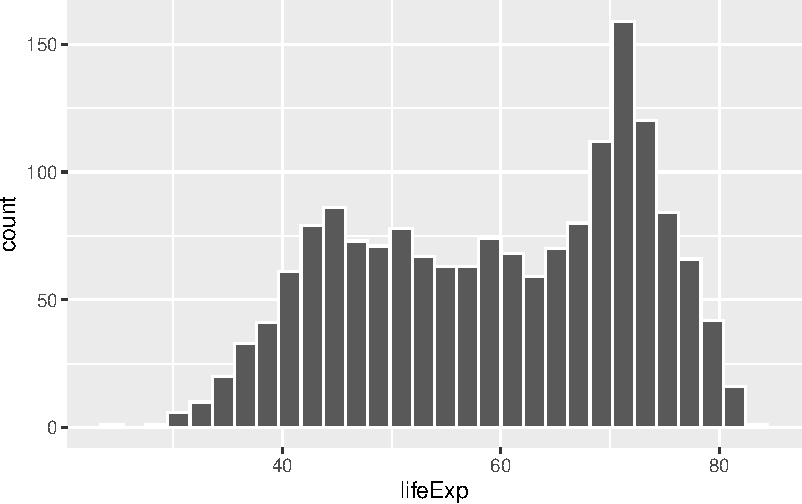
\includegraphics{06_ggplot2_files/figure-pdf/unnamed-chunk-40-1.pdf}

Notice that \texttt{color} here refers to the \emph{outline} of the
bars, rather than the bars themselves. If you want the bars themselves
to have a different color, you need to use the \texttt{fill} aesthetic.

\begin{Shaded}
\begin{Highlighting}[]
\FunctionTok{ggplot}\NormalTok{(gapminder) }\SpecialCharTok{+} 
  \FunctionTok{geom\_histogram}\NormalTok{(}\FunctionTok{aes}\NormalTok{(}\AttributeTok{x =}\NormalTok{ lifeExp), }
                 \AttributeTok{color =} \StringTok{"white"}\NormalTok{,}
                 \AttributeTok{fill =} \StringTok{"cornflowerblue"}\NormalTok{)}
\end{Highlighting}
\end{Shaded}

\begin{verbatim}
`stat_bin()` using `bins = 30`. Pick better value with `binwidth`.
\end{verbatim}

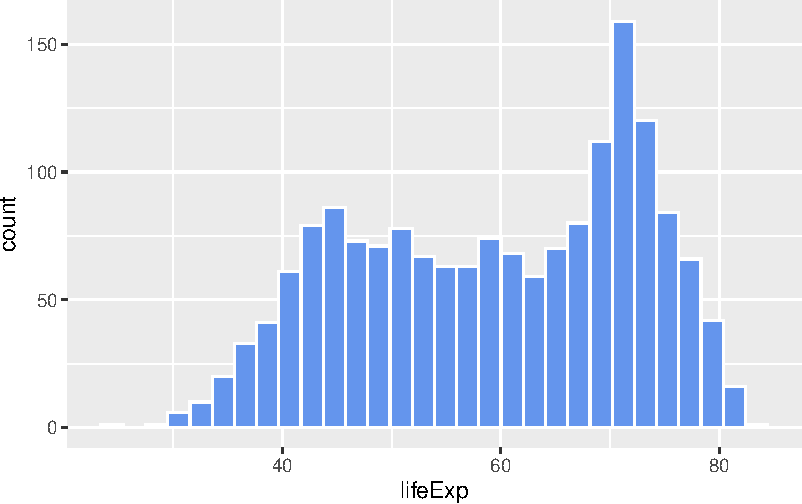
\includegraphics{06_ggplot2_files/figure-pdf/unnamed-chunk-41-1.pdf}

You can also provide a \texttt{fill} to your histogram where the bars
are colored using a categorical variable, such as \texttt{continent}:

\begin{Shaded}
\begin{Highlighting}[]
\FunctionTok{ggplot}\NormalTok{(gapminder) }\SpecialCharTok{+} 
  \FunctionTok{geom\_histogram}\NormalTok{(}\FunctionTok{aes}\NormalTok{(}\AttributeTok{x =}\NormalTok{ lifeExp, }\AttributeTok{fill =}\NormalTok{ continent), }
                 \AttributeTok{color =} \StringTok{"white"}\NormalTok{)}
\end{Highlighting}
\end{Shaded}

\begin{verbatim}
`stat_bin()` using `bins = 30`. Pick better value with `binwidth`.
\end{verbatim}

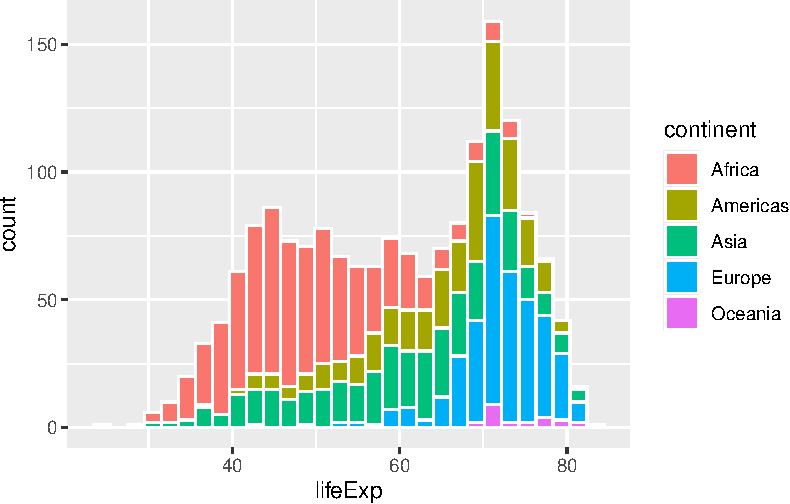
\includegraphics{06_ggplot2_files/figure-pdf/unnamed-chunk-42-1.pdf}

But be warned that these bars are \emph{``stacked''} on top of one
another, so the overall shape is the same as that of the entire variable
in the histograms above.

If you want to compare the distributions of the \texttt{lifeExp}
variable across each continent where each continent's histogram starts
from 0, you need to specify an additional argument to
\texttt{geom\_histogram()} that is \texttt{position\ =\ "identity"}.

\begin{Shaded}
\begin{Highlighting}[]
\FunctionTok{ggplot}\NormalTok{(gapminder) }\SpecialCharTok{+} 
  \FunctionTok{geom\_histogram}\NormalTok{(}\FunctionTok{aes}\NormalTok{(}\AttributeTok{x =}\NormalTok{ lifeExp, }\AttributeTok{fill =}\NormalTok{ continent), }
                 \AttributeTok{color =} \StringTok{"white"}\NormalTok{,}
                 \AttributeTok{position =} \StringTok{"identity"}\NormalTok{)}
\end{Highlighting}
\end{Shaded}

\begin{verbatim}
`stat_bin()` using `bins = 30`. Pick better value with `binwidth`.
\end{verbatim}

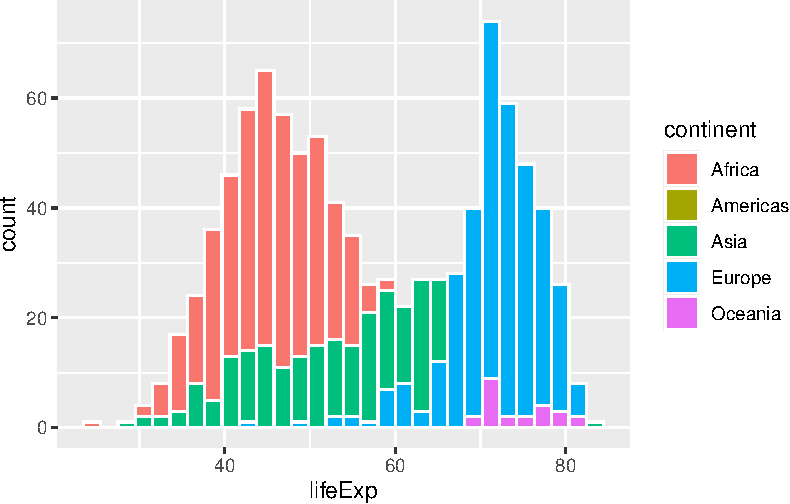
\includegraphics{06_ggplot2_files/figure-pdf/unnamed-chunk-43-1.pdf}

Now each continent's histograms start at y = 0, but because they are
opaque, it is a hard to see the distributions where they overlap.

This is another place where transparency comes in handy! If we set
\texttt{alpha\ =\ 0.5}, we can see a bit more easily how the
distributionso overlap.

\begin{Shaded}
\begin{Highlighting}[]
\FunctionTok{ggplot}\NormalTok{(gapminder) }\SpecialCharTok{+} 
  \FunctionTok{geom\_histogram}\NormalTok{(}\FunctionTok{aes}\NormalTok{(}\AttributeTok{x =}\NormalTok{ lifeExp, }\AttributeTok{fill =}\NormalTok{ continent), }
                 \AttributeTok{color =} \StringTok{"white"}\NormalTok{,}
                 \AttributeTok{position =} \StringTok{"identity"}\NormalTok{,}
                 \AttributeTok{alpha =} \FloatTok{0.5}\NormalTok{)}
\end{Highlighting}
\end{Shaded}

\begin{verbatim}
`stat_bin()` using `bins = 30`. Pick better value with `binwidth`.
\end{verbatim}

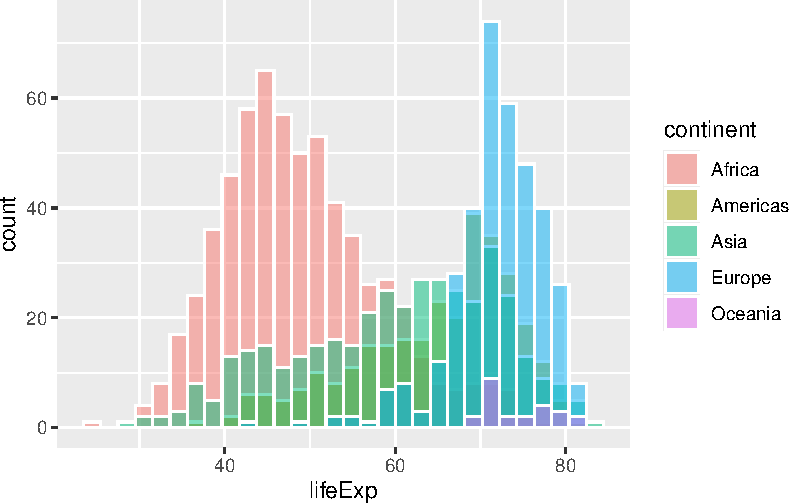
\includegraphics{06_ggplot2_files/figure-pdf/unnamed-chunk-44-1.pdf}

This plot is a bit busy though, so it might be a bit easier to just
compare two groups, such as ``Europe'' and ``Africa'':

\begin{Shaded}
\begin{Highlighting}[]
\NormalTok{gapminder }\SpecialCharTok{|\textgreater{}}
  \FunctionTok{filter}\NormalTok{(continent }\SpecialCharTok{\%in\%} \FunctionTok{c}\NormalTok{(}\StringTok{"Europe"}\NormalTok{, }\StringTok{"Africa"}\NormalTok{)) }\SpecialCharTok{|\textgreater{}}
  \FunctionTok{ggplot}\NormalTok{() }\SpecialCharTok{+} 
  \FunctionTok{geom\_histogram}\NormalTok{(}\FunctionTok{aes}\NormalTok{(}\AttributeTok{x =}\NormalTok{ lifeExp, }\AttributeTok{fill =}\NormalTok{ continent), }
                 \AttributeTok{color =} \StringTok{"white"}\NormalTok{,}
                 \AttributeTok{position =} \StringTok{"identity"}\NormalTok{,}
                 \AttributeTok{alpha =} \FloatTok{0.5}\NormalTok{)}
\end{Highlighting}
\end{Shaded}

\begin{verbatim}
`stat_bin()` using `bins = 30`. Pick better value with `binwidth`.
\end{verbatim}

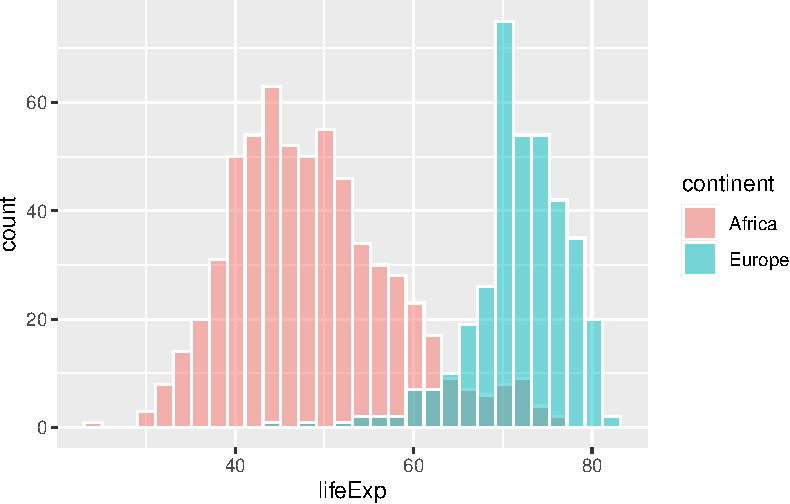
\includegraphics{06_ggplot2_files/figure-pdf/unnamed-chunk-45-1.pdf}

\subsection{Bar charts}\label{bar-charts}

A bar chart is like a histogram, but for categorical variables instead
of continuous numeric ones.

You can create a \emph{count} bar chart, by providing a categorical
(character/factor) variable as your x-aesthetic to \texttt{geom\_bar()},
which will then add up how many times each value of the categorical
variable appears and use this as the height of the bars:

\begin{Shaded}
\begin{Highlighting}[]
\CommentTok{\# create a bar chart of the continent *counts*}
\FunctionTok{ggplot}\NormalTok{(gapminder) }\SpecialCharTok{+}
  \FunctionTok{geom\_bar}\NormalTok{(}\FunctionTok{aes}\NormalTok{(}\AttributeTok{x =}\NormalTok{ continent))}
\end{Highlighting}
\end{Shaded}

\includegraphics{06_ggplot2_files/figure-pdf/unnamed-chunk-46-1.pdf}

If you want to create bar charts where you specify the height of each
bar based on a variable in your data, you want to use
\texttt{geom\_col()} instead of \texttt{geom\_bar()}.

For example, below, I create a bar chart that shows the \emph{average
life expectancy} for each continent, first you have to calculate the
average life expectancy for each continent, and then you can pipe that
into ggplot with a \texttt{geom\_col()} layer that uses
\texttt{x\ =\ continent} as the x-aesthetic that specifies how many bars
there are (and their names), and your calculated
\texttt{y\ =\ mean\_life\_exp} as the height aesthetic.

\begin{Shaded}
\begin{Highlighting}[]
\NormalTok{gapminder }\SpecialCharTok{|\textgreater{}}
  \FunctionTok{group\_by}\NormalTok{(continent) }\SpecialCharTok{|\textgreater{}}
  \FunctionTok{summarize}\NormalTok{(}\AttributeTok{mean\_life\_exp =} \FunctionTok{mean}\NormalTok{(lifeExp)) }\SpecialCharTok{|\textgreater{}}
  \FunctionTok{ggplot}\NormalTok{() }\SpecialCharTok{+}
  \FunctionTok{geom\_col}\NormalTok{(}\FunctionTok{aes}\NormalTok{(}\AttributeTok{x =}\NormalTok{ continent, }\AttributeTok{y =}\NormalTok{ mean\_life\_exp))}
\end{Highlighting}
\end{Shaded}

\includegraphics{06_ggplot2_files/figure-pdf/unnamed-chunk-47-1.pdf}

Note that like histograms, you can give each bar a color using the
\texttt{fill} aesthetic.

To give each bar a different color per continent, provide
\texttt{fill\ =\ continent} \emph{inside} the \texttt{aes()} function:

\begin{Shaded}
\begin{Highlighting}[]
\NormalTok{gapminder }\SpecialCharTok{|\textgreater{}}
  \FunctionTok{group\_by}\NormalTok{(continent) }\SpecialCharTok{|\textgreater{}}
  \FunctionTok{summarize}\NormalTok{(}\AttributeTok{mean\_life\_exp =} \FunctionTok{mean}\NormalTok{(lifeExp)) }\SpecialCharTok{|\textgreater{}}
  \FunctionTok{ggplot}\NormalTok{() }\SpecialCharTok{+}
  \FunctionTok{geom\_col}\NormalTok{(}\FunctionTok{aes}\NormalTok{(}\AttributeTok{x =}\NormalTok{ continent, }\AttributeTok{y =}\NormalTok{ mean\_life\_exp, }\AttributeTok{fill =}\NormalTok{ continent))}
\end{Highlighting}
\end{Shaded}

\includegraphics{06_ggplot2_files/figure-pdf/unnamed-chunk-48-1.pdf}

And to give each bar the same global color, provide your color to
\texttt{fill} \emph{outside} the \texttt{aes()} function:

\begin{Shaded}
\begin{Highlighting}[]
\NormalTok{gapminder }\SpecialCharTok{|\textgreater{}}
  \FunctionTok{group\_by}\NormalTok{(continent) }\SpecialCharTok{|\textgreater{}}
  \FunctionTok{summarize}\NormalTok{(}\AttributeTok{mean\_life\_exp =} \FunctionTok{mean}\NormalTok{(lifeExp)) }\SpecialCharTok{|\textgreater{}}
  \FunctionTok{ggplot}\NormalTok{() }\SpecialCharTok{+}
  \FunctionTok{geom\_col}\NormalTok{(}\FunctionTok{aes}\NormalTok{(}\AttributeTok{x =}\NormalTok{ continent, }\AttributeTok{y =}\NormalTok{ mean\_life\_exp),}
           \AttributeTok{fill =} \StringTok{"cornflowerblue"}\NormalTok{)}
\end{Highlighting}
\end{Shaded}

\includegraphics{06_ggplot2_files/figure-pdf/unnamed-chunk-49-1.pdf}

\section{Getting fancy with ggplot2}\label{getting-fancy-with-ggplot2}

Now that you've seen the most common ggplot2 layers that I typically
use, let's talk about how to do even fancier things with them.

\subsection{Transformations}\label{transformations}

You can apply log-scale transformations to your axis by adding a scale
layer. Below, the layer \texttt{scale\_x\_log10()} converts the x-axis
to a \(\log_{10}\) scale, so each break increases by an order of
magnitude rather than by a fixed amount.

\begin{Shaded}
\begin{Highlighting}[]
\FunctionTok{ggplot}\NormalTok{(gapminder\_2007) }\SpecialCharTok{+} 
  \FunctionTok{geom\_point}\NormalTok{(}\FunctionTok{aes}\NormalTok{(}\AttributeTok{x =}\NormalTok{ gdpPercap, }
                 \AttributeTok{y =}\NormalTok{ lifeExp, }
                 \AttributeTok{color =}\NormalTok{ continent)) }\SpecialCharTok{+} 
  \FunctionTok{scale\_x\_log10}\NormalTok{()}
\end{Highlighting}
\end{Shaded}

\includegraphics{06_ggplot2_files/figure-pdf/unnamed-chunk-50-1.pdf}

Because I want to keep using this plot as I show you more cool things,
I'm going to save it as a variable!

I can do this by assigning it to a new variable name like this:

\begin{Shaded}
\begin{Highlighting}[]
\NormalTok{life\_gdp\_scatter }\OtherTok{\textless{}{-}} \FunctionTok{ggplot}\NormalTok{(gapminder\_2007) }\SpecialCharTok{+} 
  \FunctionTok{geom\_point}\NormalTok{(}\FunctionTok{aes}\NormalTok{(}\AttributeTok{x =}\NormalTok{ gdpPercap, }
                 \AttributeTok{y =}\NormalTok{ lifeExp, }
                 \AttributeTok{color =}\NormalTok{ continent)) }\SpecialCharTok{+} 
  \FunctionTok{scale\_x\_log10}\NormalTok{()}
\end{Highlighting}
\end{Shaded}

As usual, when I define this variable, no output is shown, but I can
look at the object contained in this variable by typing its name:

\begin{Shaded}
\begin{Highlighting}[]
\NormalTok{life\_gdp\_scatter}
\end{Highlighting}
\end{Shaded}

\includegraphics{06_ggplot2_files/figure-pdf/unnamed-chunk-52-1.pdf}

And the super neat thing is that because this is just a ggplot object, I
can keep adding things to it!

\subsection{Labels}\label{labels}

You can clean the labels of your figure by adding a \texttt{labs()}
layer.

\begin{Shaded}
\begin{Highlighting}[]
\NormalTok{life\_gdp\_scatter }\SpecialCharTok{+} 
  \FunctionTok{labs}\NormalTok{(}\AttributeTok{x =} \StringTok{"GDP per capita"}\NormalTok{, }
       \AttributeTok{y =} \StringTok{"Life expectancy"}\NormalTok{, }
       \AttributeTok{title =} \StringTok{"GDP per cap vs life expectancy"}\NormalTok{)}
\end{Highlighting}
\end{Shaded}

\includegraphics{06_ggplot2_files/figure-pdf/unnamed-chunk-53-1.pdf}

This is equivalent to replacing \texttt{life\_gdp\_scatter} with the
code that was used to define it

\begin{Shaded}
\begin{Highlighting}[]
\FunctionTok{ggplot}\NormalTok{(gapminder\_2007) }\SpecialCharTok{+} 
  \FunctionTok{geom\_point}\NormalTok{(}\FunctionTok{aes}\NormalTok{(}\AttributeTok{x =}\NormalTok{ gdpPercap, }
                 \AttributeTok{y =}\NormalTok{ lifeExp, }
                 \AttributeTok{color =}\NormalTok{ continent)) }\SpecialCharTok{+} 
  \FunctionTok{scale\_x\_log10}\NormalTok{() }\SpecialCharTok{+}
  \FunctionTok{labs}\NormalTok{(}\AttributeTok{x =} \StringTok{"GDP per capita"}\NormalTok{, }
       \AttributeTok{y =} \StringTok{"Life expectancy"}\NormalTok{, }
       \AttributeTok{title =} \StringTok{"GDP per cap vs life expectancy"}\NormalTok{)}
\end{Highlighting}
\end{Shaded}

\includegraphics{06_ggplot2_files/figure-pdf/unnamed-chunk-54-1.pdf}

And I'm going to update my scatterplot object to contain these new
labels:

\begin{Shaded}
\begin{Highlighting}[]
\NormalTok{life\_gdp\_scatter }\OtherTok{\textless{}{-}}\NormalTok{ life\_gdp\_scatter }\SpecialCharTok{+} 
  \FunctionTok{labs}\NormalTok{(}\AttributeTok{x =} \StringTok{"GDP per capita"}\NormalTok{, }
       \AttributeTok{y =} \StringTok{"Life expectancy"}\NormalTok{, }
       \AttributeTok{title =} \StringTok{"GDP per cap vs life expectancy"}\NormalTok{)}
\end{Highlighting}
\end{Shaded}

\subsection{Themes}\label{themes}

Next, I want to give my figure a theme by adding a themes layer. There
are a lot of theme options. My favorite is \texttt{theme\_classic()}:

\begin{Shaded}
\begin{Highlighting}[]
\NormalTok{life\_gdp\_scatter }\SpecialCharTok{+} \FunctionTok{theme\_classic}\NormalTok{()}
\end{Highlighting}
\end{Shaded}

\includegraphics{06_ggplot2_files/figure-pdf/unnamed-chunk-56-1.pdf}

Another popular one is \texttt{theme\_bw()}:

\begin{Shaded}
\begin{Highlighting}[]
\NormalTok{life\_gdp\_scatter }\SpecialCharTok{+} \FunctionTok{theme\_bw}\NormalTok{()}
\end{Highlighting}
\end{Shaded}

\includegraphics{06_ggplot2_files/figure-pdf/unnamed-chunk-57-1.pdf}

and \texttt{theme\_minimal()}:

\begin{Shaded}
\begin{Highlighting}[]
\NormalTok{life\_gdp\_scatter }\SpecialCharTok{+} \FunctionTok{theme\_minimal}\NormalTok{()}
\end{Highlighting}
\end{Shaded}

\includegraphics{06_ggplot2_files/figure-pdf/unnamed-chunk-58-1.pdf}

But there are
\href{https://ggplot2.tidyverse.org/reference/ggtheme.html}{lots of
others too}.

\subsection{Faceted grids}\label{faceted-grids}

The last neat ggplot2 thing I want to show you is how to create a grid
of plots using \texttt{facet\_wrap()}.

If I have a bunch of line plots on the same plot like this:

\begin{Shaded}
\begin{Highlighting}[]
\NormalTok{gapminder }\SpecialCharTok{|\textgreater{}}
  \FunctionTok{filter}\NormalTok{(continent }\SpecialCharTok{==} \StringTok{"Americas"}\NormalTok{) }\SpecialCharTok{|\textgreater{}}
  \FunctionTok{ggplot}\NormalTok{() }\SpecialCharTok{+} 
  \FunctionTok{geom\_line}\NormalTok{(}\FunctionTok{aes}\NormalTok{(}\AttributeTok{x =}\NormalTok{ year, }
                \AttributeTok{y =}\NormalTok{ lifeExp, }
                \AttributeTok{group =}\NormalTok{ country))}
\end{Highlighting}
\end{Shaded}

\includegraphics{06_ggplot2_files/figure-pdf/unnamed-chunk-59-1.pdf}

I might find myself wishing that I had a separate plot for each country,
but I don't want to actually write the code to create a separate line
plot for each country manually.

Fortunately, \texttt{facet\_wrap()} (and \texttt{facet\_grid()}) can do
this for me. Below I take the exact same code and I add a
\texttt{facet\_wrap()} layer where I specify which categorical variable
in my data I want to use to specify the different plot panels (I write
\texttt{\textasciitilde{}country} to create a separate panel for each
value in country). This is essentially just taking each line in the plot
above and giving it its own plot. Each plot will inherit the aesthetic
properties of the \texttt{geom\_line()} layer.

\begin{Shaded}
\begin{Highlighting}[]
\NormalTok{gapminder }\SpecialCharTok{|\textgreater{}}
  \FunctionTok{filter}\NormalTok{(continent }\SpecialCharTok{==} \StringTok{"Americas"}\NormalTok{) }\SpecialCharTok{|\textgreater{}}
  \FunctionTok{ggplot}\NormalTok{() }\SpecialCharTok{+} 
  \FunctionTok{geom\_line}\NormalTok{(}\FunctionTok{aes}\NormalTok{(}\AttributeTok{x =}\NormalTok{ year, }
                \AttributeTok{y =}\NormalTok{ lifeExp)) }\SpecialCharTok{+}
  \FunctionTok{facet\_wrap}\NormalTok{(}\SpecialCharTok{\textasciitilde{}}\NormalTok{country)}
\end{Highlighting}
\end{Shaded}

\includegraphics{06_ggplot2_files/figure-pdf/unnamed-chunk-60-1.pdf}

This plot is all cramped, but if I add some
\texttt{\#\textbar{}\ fig-height} and \texttt{\#\textbar{}\ fig-width}
options to the top of my code chunk, I can control its size, such as

\begin{Shaded}
\begin{Highlighting}[]
\InformationTok{\textasciigrave{}\textasciigrave{}\textasciigrave{}\{r\}}
\InformationTok{\#| fig{-}height: 8}
\InformationTok{\#| fig{-}width: 8}
\InformationTok{gapminder |\textgreater{}}
\InformationTok{  filter(continent == "Americas") |\textgreater{}}
\InformationTok{  ggplot() + }
\InformationTok{  geom\_line(aes(x = year, }
\InformationTok{                y = lifeExp)) +}
\InformationTok{  facet\_wrap(\textasciitilde{}country)}
\InformationTok{\textasciigrave{}\textasciigrave{}\textasciigrave{}}
\end{Highlighting}
\end{Shaded}

\includegraphics{06_ggplot2_files/figure-pdf/unnamed-chunk-61-1.pdf}

Note that I also rotated my x-axis text 90 degrees using a
\texttt{theme()} layer. If you want to start truly customizing your your
ggplots, you're going to get intimately familiar with the
\texttt{theme()} layer options.

You can also specify the number of columns in your faceted grid using
the \texttt{ncol} argument:

\begin{Shaded}
\begin{Highlighting}[]
\NormalTok{gapminder }\SpecialCharTok{|\textgreater{}}
  \FunctionTok{filter}\NormalTok{(continent }\SpecialCharTok{==} \StringTok{"Americas"}\NormalTok{) }\SpecialCharTok{|\textgreater{}}
  \FunctionTok{ggplot}\NormalTok{() }\SpecialCharTok{+} 
  \FunctionTok{geom\_line}\NormalTok{(}\FunctionTok{aes}\NormalTok{(}\AttributeTok{x =}\NormalTok{ year, }
                \AttributeTok{y =}\NormalTok{ lifeExp)) }\SpecialCharTok{+}
  \FunctionTok{facet\_wrap}\NormalTok{(}\SpecialCharTok{\textasciitilde{}}\NormalTok{country, }\AttributeTok{ncol =} \DecValTok{4}\NormalTok{)}
\end{Highlighting}
\end{Shaded}

\includegraphics{06_ggplot2_files/figure-pdf/unnamed-chunk-62-1.pdf}

\section{Exercise}

Create a faceted grid of scatterplots of \texttt{lifeExp} against
\texttt{gdpPercap} in 2007 for each continent. Do some fancy things to
make your plot sparkle!

\section{Solution}

Here is a base plot without any fun:

\begin{Shaded}
\begin{Highlighting}[]
\NormalTok{gapminder\_2007 }\SpecialCharTok{|\textgreater{}}
  \FunctionTok{ggplot}\NormalTok{() }\SpecialCharTok{+}
  \FunctionTok{geom\_point}\NormalTok{(}\FunctionTok{aes}\NormalTok{(}\AttributeTok{x =}\NormalTok{ lifeExp, }\AttributeTok{y =}\NormalTok{ gdpPercap)) }\SpecialCharTok{+}
  \FunctionTok{facet\_wrap}\NormalTok{(}\SpecialCharTok{\textasciitilde{}}\NormalTok{continent)}
\end{Highlighting}
\end{Shaded}

\includegraphics{06_ggplot2_files/figure-pdf/unnamed-chunk-63-1.pdf}

Here is a plot with some fun:

\begin{Shaded}
\begin{Highlighting}[]
\NormalTok{gapminder\_2007 }\SpecialCharTok{|\textgreater{}}
  \FunctionTok{ggplot}\NormalTok{() }\SpecialCharTok{+}
  \FunctionTok{geom\_point}\NormalTok{(}\FunctionTok{aes}\NormalTok{(}\AttributeTok{x =}\NormalTok{ lifeExp, }
                 \AttributeTok{y =}\NormalTok{ gdpPercap,}
                 \AttributeTok{size =}\NormalTok{ pop,}
                 \AttributeTok{color =}\NormalTok{ continent),}
             \AttributeTok{alpha =} \FloatTok{0.5}\NormalTok{) }\SpecialCharTok{+}
  \FunctionTok{scale\_x\_log10}\NormalTok{() }\SpecialCharTok{+}
  \FunctionTok{scale\_y\_log10}\NormalTok{() }\SpecialCharTok{+}
  \FunctionTok{theme\_minimal}\NormalTok{() }\SpecialCharTok{+}
  \FunctionTok{facet\_wrap}\NormalTok{(}\SpecialCharTok{\textasciitilde{}}\NormalTok{continent) }\SpecialCharTok{+}
  \FunctionTok{labs}\NormalTok{(}\AttributeTok{x =} \StringTok{"Life Expectancy"}\NormalTok{,}
       \AttributeTok{y =} \StringTok{"GDP per Capita"}\NormalTok{,}
       \AttributeTok{size =} \StringTok{"Population"}\NormalTok{,}
       \AttributeTok{color =} \StringTok{"Continent"}\NormalTok{) }
\end{Highlighting}
\end{Shaded}

\includegraphics{06_ggplot2_files/figure-pdf/unnamed-chunk-64-1.pdf}




\end{document}
